% Options for packages loaded elsewhere
% Options for packages loaded elsewhere
\PassOptionsToPackage{unicode}{hyperref}
\PassOptionsToPackage{hyphens}{url}
\PassOptionsToPackage{dvipsnames,svgnames,x11names}{xcolor}
%
\documentclass[
  russian,
  11pt,
  a4paper,
  open=any]{scrbook}
\usepackage{xcolor}
\usepackage[top=18mm,bottom=20mm,inner=20mm,outer=50mm,marginparwidth=36mm,marginparsep=6mm,headheight=6mm,headsep=5mm,footskip=9mm]{geometry}
\usepackage{amsmath,amssymb}
\setcounter{secnumdepth}{3}
\usepackage{iftex}
\ifPDFTeX
  \usepackage[T1]{fontenc}
  \usepackage[utf8]{inputenc}
  \usepackage{textcomp} % provide euro and other symbols
\else % if luatex or xetex
  \usepackage{unicode-math} % this also loads fontspec
  \defaultfontfeatures{Scale=MatchLowercase}
  \defaultfontfeatures[\rmfamily]{Ligatures=TeX,Scale=1}
\fi
\usepackage{lmodern}
\ifPDFTeX\else
  % xetex/luatex font selection
\fi
% Use upquote if available, for straight quotes in verbatim environments
\IfFileExists{upquote.sty}{\usepackage{upquote}}{}
\IfFileExists{microtype.sty}{% use microtype if available
  \usepackage[]{microtype}
  \UseMicrotypeSet[protrusion]{basicmath} % disable protrusion for tt fonts
}{}
\makeatletter
\@ifundefined{KOMAClassName}{% if non-KOMA class
  \IfFileExists{parskip.sty}{%
    \usepackage{parskip}
  }{% else
    \setlength{\parindent}{0pt}
    \setlength{\parskip}{6pt plus 2pt minus 1pt}}
}{% if KOMA class
  \KOMAoptions{parskip=half}}
\makeatother
% Make \paragraph and \subparagraph free-standing
\makeatletter
\ifx\paragraph\undefined\else
  \let\oldparagraph\paragraph
  \renewcommand{\paragraph}{
    \@ifstar
      \xxxParagraphStar
      \xxxParagraphNoStar
  }
  \newcommand{\xxxParagraphStar}[1]{\oldparagraph*{#1}\mbox{}}
  \newcommand{\xxxParagraphNoStar}[1]{\oldparagraph{#1}\mbox{}}
\fi
\ifx\subparagraph\undefined\else
  \let\oldsubparagraph\subparagraph
  \renewcommand{\subparagraph}{
    \@ifstar
      \xxxSubParagraphStar
      \xxxSubParagraphNoStar
  }
  \newcommand{\xxxSubParagraphStar}[1]{\oldsubparagraph*{#1}\mbox{}}
  \newcommand{\xxxSubParagraphNoStar}[1]{\oldsubparagraph{#1}\mbox{}}
\fi
\makeatother

\usepackage{color}
\usepackage{fancyvrb}
\newcommand{\VerbBar}{|}
\newcommand{\VERB}{\Verb[commandchars=\\\{\}]}
\DefineVerbatimEnvironment{Highlighting}{Verbatim}{commandchars=\\\{\}}
% Add ',fontsize=\small' for more characters per line
\usepackage{framed}
\definecolor{shadecolor}{RGB}{241,243,245}
\newenvironment{Shaded}{\begin{snugshade}}{\end{snugshade}}
\newcommand{\AlertTok}[1]{\textcolor[rgb]{0.68,0.00,0.00}{#1}}
\newcommand{\AnnotationTok}[1]{\textcolor[rgb]{0.37,0.37,0.37}{#1}}
\newcommand{\AttributeTok}[1]{\textcolor[rgb]{0.40,0.45,0.13}{#1}}
\newcommand{\BaseNTok}[1]{\textcolor[rgb]{0.68,0.00,0.00}{#1}}
\newcommand{\BuiltInTok}[1]{\textcolor[rgb]{0.00,0.23,0.31}{#1}}
\newcommand{\CharTok}[1]{\textcolor[rgb]{0.13,0.47,0.30}{#1}}
\newcommand{\CommentTok}[1]{\textcolor[rgb]{0.37,0.37,0.37}{#1}}
\newcommand{\CommentVarTok}[1]{\textcolor[rgb]{0.37,0.37,0.37}{\textit{#1}}}
\newcommand{\ConstantTok}[1]{\textcolor[rgb]{0.56,0.35,0.01}{#1}}
\newcommand{\ControlFlowTok}[1]{\textcolor[rgb]{0.00,0.23,0.31}{\textbf{#1}}}
\newcommand{\DataTypeTok}[1]{\textcolor[rgb]{0.68,0.00,0.00}{#1}}
\newcommand{\DecValTok}[1]{\textcolor[rgb]{0.68,0.00,0.00}{#1}}
\newcommand{\DocumentationTok}[1]{\textcolor[rgb]{0.37,0.37,0.37}{\textit{#1}}}
\newcommand{\ErrorTok}[1]{\textcolor[rgb]{0.68,0.00,0.00}{#1}}
\newcommand{\ExtensionTok}[1]{\textcolor[rgb]{0.00,0.23,0.31}{#1}}
\newcommand{\FloatTok}[1]{\textcolor[rgb]{0.68,0.00,0.00}{#1}}
\newcommand{\FunctionTok}[1]{\textcolor[rgb]{0.28,0.35,0.67}{#1}}
\newcommand{\ImportTok}[1]{\textcolor[rgb]{0.00,0.46,0.62}{#1}}
\newcommand{\InformationTok}[1]{\textcolor[rgb]{0.37,0.37,0.37}{#1}}
\newcommand{\KeywordTok}[1]{\textcolor[rgb]{0.00,0.23,0.31}{\textbf{#1}}}
\newcommand{\NormalTok}[1]{\textcolor[rgb]{0.00,0.23,0.31}{#1}}
\newcommand{\OperatorTok}[1]{\textcolor[rgb]{0.37,0.37,0.37}{#1}}
\newcommand{\OtherTok}[1]{\textcolor[rgb]{0.00,0.23,0.31}{#1}}
\newcommand{\PreprocessorTok}[1]{\textcolor[rgb]{0.68,0.00,0.00}{#1}}
\newcommand{\RegionMarkerTok}[1]{\textcolor[rgb]{0.00,0.23,0.31}{#1}}
\newcommand{\SpecialCharTok}[1]{\textcolor[rgb]{0.37,0.37,0.37}{#1}}
\newcommand{\SpecialStringTok}[1]{\textcolor[rgb]{0.13,0.47,0.30}{#1}}
\newcommand{\StringTok}[1]{\textcolor[rgb]{0.13,0.47,0.30}{#1}}
\newcommand{\VariableTok}[1]{\textcolor[rgb]{0.07,0.07,0.07}{#1}}
\newcommand{\VerbatimStringTok}[1]{\textcolor[rgb]{0.13,0.47,0.30}{#1}}
\newcommand{\WarningTok}[1]{\textcolor[rgb]{0.37,0.37,0.37}{\textit{#1}}}

\usepackage{longtable,booktabs,array}
\newcounter{none} % for unnumbered tables
\usepackage{calc} % for calculating minipage widths
% Correct order of tables after \paragraph or \subparagraph
\usepackage{etoolbox}
\makeatletter
\patchcmd\longtable{\par}{\if@noskipsec\mbox{}\fi\par}{}{}
\makeatother
% Allow footnotes in longtable head/foot
\IfFileExists{footnotehyper.sty}{\usepackage{footnotehyper}}{\usepackage{footnote}}
\makesavenoteenv{longtable}
\usepackage{graphicx}
\makeatletter
\newsavebox\pandoc@box
\newcommand*\pandocbounded[1]{% scales image to fit in text height/width
  \sbox\pandoc@box{#1}%
  \Gscale@div\@tempa{\textheight}{\dimexpr\ht\pandoc@box+\dp\pandoc@box\relax}%
  \Gscale@div\@tempb{\linewidth}{\wd\pandoc@box}%
  \ifdim\@tempb\p@<\@tempa\p@\let\@tempa\@tempb\fi% select the smaller of both
  \ifdim\@tempa\p@<\p@\scalebox{\@tempa}{\usebox\pandoc@box}%
  \else\usebox{\pandoc@box}%
  \fi%
}
% Set default figure placement to htbp
\def\fps@figure{htbp}
\makeatother


% definitions for citeproc citations
\NewDocumentCommand\citeproctext{}{}
\NewDocumentCommand\citeproc{mm}{%
  \begingroup\def\citeproctext{#2}\cite{#1}\endgroup}
\makeatletter
 % allow citations to break across lines
 \let\@cite@ofmt\@firstofone
 % avoid brackets around text for \cite:
 \def\@biblabel#1{}
 \def\@cite#1#2{{#1\if@tempswa , #2\fi}}
\makeatother
\newlength{\cslhangindent}
\setlength{\cslhangindent}{1.5em}
\newlength{\csllabelwidth}
\setlength{\csllabelwidth}{3em}
\newenvironment{CSLReferences}[2] % #1 hanging-indent, #2 entry-spacing
 {\begin{list}{}{%
  \setlength{\itemindent}{0pt}
  \setlength{\leftmargin}{0pt}
  \setlength{\parsep}{0pt}
  % turn on hanging indent if param 1 is 1
  \ifodd #1
   \setlength{\leftmargin}{\cslhangindent}
   \setlength{\itemindent}{-1\cslhangindent}
  \fi
  % set entry spacing
  \setlength{\itemsep}{#2\baselineskip}}}
 {\end{list}}
\usepackage{calc}
\newcommand{\CSLBlock}[1]{\hfill\break\parbox[t]{\linewidth}{\strut\ignorespaces#1\strut}}
\newcommand{\CSLLeftMargin}[1]{\parbox[t]{\csllabelwidth}{\strut#1\strut}}
\newcommand{\CSLRightInline}[1]{\parbox[t]{\linewidth - \csllabelwidth}{\strut#1\strut}}
\newcommand{\CSLIndent}[1]{\hspace{\cslhangindent}#1}

\ifLuaTeX
\usepackage[bidi=basic,shorthands=off,provide=*]{babel}
\else
\usepackage[bidi=default,shorthands=off,provide=*]{babel}
\fi
\ifLuaTeX
  \usepackage{selnolig} % disable illegal ligatures
\fi


\setlength{\emergencystretch}{3em} % prevent overfull lines

\providecommand{\tightlist}{%
  \setlength{\itemsep}{0pt}\setlength{\parskip}{0pt}}



 


% Canonical PDF foundation for books in the NeutrinoHit universe.

\usepackage{fontspec}
\usepackage{polyglossia}
\usepackage{unicode-math}
\usepackage{amsmath}
\usepackage{mathtools}
\usepackage{graphicx}
\usepackage{float}
\usepackage{booktabs}
\usepackage{longtable}
\usepackage{array}
\usepackage{microtype}
\usepackage{hyperref}
\usepackage{tikz}
\usepackage[most]{tcolorbox}
\usepackage{caption}
\usepackage{ragged2e}
\usepackage{etoc}
\usepackage[automark]{scrlayer-scrpage}

\defaultfontfeatures{Ligatures=TeX, Scale=MatchLowercase}
\setmainfont{Libertinus Serif}
\setsansfont{Libertinus Sans}
\setmonofont{Libertinus Mono}[Scale=0.9]
\setmathfont{Libertinus Math}

\definecolor{BookInk}{HTML}{18262F}
\definecolor{BookInkSoft}{HTML}{42545F}
\definecolor{BookMuted}{HTML}{687984}
\definecolor{BookPaper}{HTML}{FFFFFF}
\definecolor{BookCanvas}{HTML}{F4F6F7}
\definecolor{BookLine}{HTML}{D9E0E3}
\definecolor{BookLineStrong}{HTML}{BCC9CE}
\definecolor{BookTeal}{HTML}{0F6972}
\definecolor{BookTealDark}{HTML}{094B52}
\definecolor{BookTealSoft}{HTML}{E8F1F2}
\definecolor{BookBlue}{HTML}{2F6F9F}
\definecolor{BookBlueSoft}{HTML}{EDF3FA}
\definecolor{BookCoral}{HTML}{C7472F}
\definecolor{BookCoralSoft}{HTML}{FAEEEB}
\definecolor{BookGold}{HTML}{B97817}
\definecolor{BookGoldSoft}{HTML}{FBF3E4}
\definecolor{BookBiography}{HTML}{465B8C}
\definecolor{BookBiographySoft}{HTML}{F0F2F8}
\definecolor{BookMargin}{HTML}{F1F3F4}

% Compatibility aliases let established books keep their local command style.
\colorlet{bookInk}{BookInk}
\colorlet{bookMuted}{BookMuted}
\colorlet{bookTeal}{BookTeal}
\colorlet{bookTealSoft}{BookTealSoft}
\colorlet{bookBlue}{BookBlue}
\colorlet{bookBlueSoft}{BookBlueSoft}
\colorlet{bookCoral}{BookCoral}
\colorlet{bookCoralSoft}{BookCoralSoft}
\colorlet{bookBiography}{BookBiography}
\colorlet{bookBiographySoft}{BookBiographySoft}
\colorlet{bookMargin}{BookMargin}

\setlength{\emergencystretch}{3em}
\raggedbottom

\hypersetup{
  pdfborder={0 0 0},
  colorlinks=true,
  linkcolor=BookTeal,
  citecolor=BookTeal,
  urlcolor=BookTeal
}

% Shared semantic boxes used by biographies, media cards, notes and exercises.
\newtcolorbox{semanticpdfbox}[1][]{
  enhanced,
  breakable,
  sharp corners,
  colback=BookTealSoft,
  colframe=BookTeal,
  boxrule=0pt,
  borderline west={1.2mm}{0pt}{BookTeal},
  left=4mm,
  right=3mm,
  top=2mm,
  bottom=2mm,
  #1
}

% Reusable ordered process. Source nodes are generic process-flow/process-step
% Divs; the Lua filter maps them to these vertical PDF cards.
\newenvironment{bookprocessflow}{%
  \par\vspace{2mm}\begingroup
  \setlength{\parindent}{0pt}%
}{%
  \endgroup\par\vspace{2mm}%
}

\newcommand{\BookProcessBadge}[1]{%
  \tikz[baseline=(bookprocessnumber.base)]{%
    \node[
      circle,
      fill=BookTeal,
      text=white,
      minimum size=8mm,
      inner sep=0pt,
      font=\sffamily\bfseries\footnotesize
    ] (bookprocessnumber) {#1};%
  }%
}

\newtcolorbox{bookprocessstep}[2][]{
  enhanced,
  breakable,
  sharp corners,
  colback=BookPaper,
  colframe=BookLineStrong,
  boxrule=0.35pt,
  borderline west={1.2mm}{0pt}{BookTeal},
  left=4mm,
  right=3mm,
  top=2mm,
  bottom=2mm,
  before skip=2pt,
  after skip=2pt,
  title={\BookProcessBadge{#1}\hspace{2.5mm}#2},
  colbacktitle=BookPaper,
  coltitle=BookInk,
  fonttitle=\sffamily\bfseries,
  titlerule=0pt
}

\newcommand{\BookProcessConnector}{%
  \par\nopagebreak[4]
  \begin{center}
    \vspace{-1mm}%
    {\color{BookTeal}\Large$\downarrow$}%
    \vspace{-1mm}%
  \end{center}
  \nopagebreak[4]
}

% Public labels and colour hook. A book changes these without copying the
% layout machinery: for example, "Лекция" in the neutrino book and "Глава"
% in the statistics book.
\providecommand{\bookchaptercolor}{BookTeal}
\newcommand{\BookChapterLabel}{Глава}
\newcommand{\BookPartLabel}{РАЗДЕЛ КНИГИ}
\newcommand{\BookPartContentsLabel}{Главы}
\newcommand{\BookTocChapterLabel}{Глава}

\clearpairofpagestyles
\ihead{\headmark}
\newcommand{\BookHeaderPage}{\ifnum\value{chapter}=0\pagemark\fi}
\ohead{\BookHeaderPage}
\setkomafont{pageheadfoot}{\small\sffamily\color{BookMuted}}
\setkomafont{pagehead}{\small\sffamily\color{BookInk}}
\KOMAoptions{headsepline=0.35pt}
\addtokomafont{chapter}{\sffamily\color{BookInk}}
\addtokomafont{section}{\sffamily\color{BookInk}}
\addtokomafont{subsection}{\sffamily\color{BookInk}}

% Numbered chapter opener with a local table of contents.
\renewcommand*{\chapterformat}{}
\renewcommand*{\chapterlinesformat}[3]{%
  \ifnum\value{chapter}>0\relax
    \parbox[t]{\linewidth}{%
      {\sffamily\bfseries\color{\bookchaptercolor}%
       \fontsize{15}{18}\selectfont \BookChapterLabel~\thechapter\par}%
      \vspace{7mm}%
      {\sffamily\bfseries\color{BookInk}%
       \fontsize{34}{38}\selectfont #3\par}%
      \vspace{9mm}%
      {\color{\bookchaptercolor}\rule{\linewidth}{1.3mm}}%
    }%
  \else
    \parbox[t]{\linewidth}{#3}%
  \fi
}
\RedeclareSectionCommand[beforeskip=10mm,afterskip=0pt]{chapter}

% Part opener with the list of chapters belonging to the current part.
\renewcommand*{\partformat}{}
\renewcommand*{\partlineswithprefixformat}[3]{%
  \parbox[t]{\linewidth}{%
    {\sffamily\bfseries\color{\bookchaptercolor}%
     \fontsize{13}{16}\selectfont \BookPartLabel\par}%
    \vspace{9mm}%
    {\sffamily\bfseries\color{BookInk}%
     \fontsize{32}{37}\selectfont #3\par}%
    \vspace{11mm}%
    {\color{\bookchaptercolor}\rule{\linewidth}{1.5mm}}\par
    \vspace{13mm}%
    {\sffamily\bfseries\color{BookInk}%
     \fontsize{18}{22}\selectfont \BookPartContentsLabel\par}%
    \vspace{3mm}%
    {\color{\bookchaptercolor}\rule{18mm}{0.8mm}}\par
    \vspace{5mm}%
    \begingroup
      \normalfont
      \setlength{\parindent}{0pt}%
      \etocsettocstyle{}{}%
      \etocsetnexttocdepth{chapter}%
      \localtableofcontents
    \endgroup
  }%
}
\RedeclareSectionCommand[beforeskip=20mm,afterskip=0pt]{part}

\newcommand{\BookHidePartNumber}[1]{}
\newcommand{\BookChapterTocNumber}[1]{\BookTocChapterLabel~#1}
\DeclareTOCStyleEntry[numwidth=0pt,entrynumberformat=\BookHidePartNumber]{tocline}{part}
\DeclareTOCStyleEntry[numwidth=5.6em,entrynumberformat=\BookChapterTocNumber]{tocline}{chapter}

\newcommand{\bookchapteropeningcontents}{%
  \vspace{14mm}%
  \noindent
  {\sffamily\bfseries\color{BookInk}\fontsize{18}{22}\selectfont
   Содержание\par}%
  \vspace{3mm}%
  {\color{\bookchaptercolor}\rule{18mm}{0.8mm}}%
  \vspace{5mm}%
  \begingroup
    \setlength{\parindent}{0pt}%
    \etocsettocstyle{}{}%
    \etocsetnexttocdepth{section}%
    \localtableofcontents
  \endgroup
  \vfill
  \clearpage
}

% Outer navigation rail and circular page number. Dimensions are shared; the
% colour follows the current part through \bookchaptercolor.
\newif\ifbookpagenavigator
\bookpagenavigatortrue
\newlength{\bookpagerailwidth}
\newlength{\bookpagerailcenter}
\newlength{\bookpagetabheight}
\newlength{\bookpagetabcenter}
\newlength{\bookpagenumberdiameter}
\setlength{\bookpagerailwidth}{48mm}
\setlength{\bookpagerailcenter}{24mm}
\setlength{\bookpagetabheight}{28mm}
\setlength{\bookpagetabcenter}{14mm}
\setlength{\bookpagenumberdiameter}{17mm}
\newcommand{\bookpagerailcolor}{BookMargin}
\newcommand{\bookpagetabcolor}{\bookchaptercolor}
\newcommand{\bookpagenumberfill}{white}
\newcommand{\bookpagenumbercolor}{\bookchaptercolor}

\tikzset{
  book page rail/.style={fill=\bookpagerailcolor,draw=none},
  book page tab/.style={fill=\bookpagetabcolor,draw=none},
  book page number/.style={
    circle,
    fill=\bookpagenumberfill,
    draw=none,
    minimum size=\bookpagenumberdiameter,
    inner sep=0pt,
    font=\sffamily\bfseries\fontsize{22}{22}\selectfont,
    text=\bookpagenumbercolor
  }
}

\newcommand{\BookPageNavigatorLeft}{%
  \path[book page rail]
    (current page.north west) rectangle
    ([xshift=\bookpagerailwidth]current page.south west);
  \path[book page tab]
    (current page.north west) rectangle
    ([xshift=\bookpagerailwidth,yshift=-\bookpagetabheight]current page.north west);
  \node[book page number]
    at ([xshift=\bookpagerailcenter,yshift=-\bookpagetabcenter]current page.north west)
    {\thepage};
}

\newcommand{\BookPageNavigatorRight}{%
  \path[book page rail]
    ([xshift=-\bookpagerailwidth]current page.north east) rectangle
    (current page.south east);
  \path[book page tab]
    ([xshift=-\bookpagerailwidth]current page.north east) rectangle
    ([yshift=-\bookpagetabheight]current page.north east);
  \node[book page number]
    at ([xshift=-\bookpagerailcenter,yshift=-\bookpagetabcenter]current page.north east)
    {\thepage};
}

\newcommand{\BookRenderPageNavigator}{%
  \ifbookpagenavigator
    \ifnum\value{chapter}>0\relax
      \begin{tikzpicture}[remember picture,overlay]
        \ifodd\value{page}
          \BookPageNavigatorRight
        \else
          \BookPageNavigatorLeft
        \fi
      \end{tikzpicture}%
    \fi
  \fi
}
\AddToHook{shipout/background}{\BookRenderPageNavigator}
\setmainlanguage{russian}
\setotherlanguage{english}
\PolyglossiaSetup{russian}{
  bcp47=ru,
  scripttag=cyrl,
  langtag=RUS,
  hyphennames={russian},
  hyphenmins={2,2},
  frenchspacing=true,
  indentfirst=true
}
% PDF visual theme for the statistical-analysis-course book.
% It mirrors the palette and visual language from assets/styles/book.css,
% while keeping the PDF close to the supplied reference edition.

\usepackage[most]{tcolorbox}
\usepackage{scrlayer-scrpage}
\usepackage{tikz}
\usepackage{caption}
\usepackage{colortbl}
\usepackage{array}
\usepackage{enumitem}
\usepackage{etoolbox}
\usepackage{ragged2e}

% -----------------------------------------------------------------------------
% Palette (same core colors as book.css)
% -----------------------------------------------------------------------------
\definecolor{BookInk}{HTML}{18262F}
\definecolor{BookInkSoft}{HTML}{42545F}
\definecolor{BookMuted}{HTML}{687984}
\definecolor{BookPaper}{HTML}{FFFFFF}
\definecolor{BookCanvas}{HTML}{F4F6F7}
\definecolor{BookLine}{HTML}{D9E0E3}
\definecolor{BookLineStrong}{HTML}{BCC9CE}
\definecolor{BookTeal}{HTML}{0F6972}
\definecolor{BookTealDark}{HTML}{094B52}
\definecolor{BookTealSoft}{HTML}{E7F1F1}
\definecolor{BookCoral}{HTML}{C7472F}
\definecolor{BookCoralSoft}{HTML}{F8ECE9}
\definecolor{BookGold}{HTML}{B97817}
\definecolor{BookGoldSoft}{HTML}{FBF3E4}
\definecolor{BookBlue}{HTML}{2A5EA8}
\definecolor{BookBiography}{HTML}{465B8C}
\definecolor{BookBiographySoft}{HTML}{F0F2F8}
% The HTML page uses a stronger sky blue. The reference PDF intentionally uses
% a paler fill for long derivations, so that equations remain comfortable to read.
\definecolor{BookBlueSoftPDF}{HTML}{EEF4FB}
\definecolor{BookFigureSoft}{HTML}{F9FBFB}
\definecolor{BookGallerySoft}{HTML}{FBFCFC}
\definecolor{BookTableStripe}{HTML}{F7F9FA}

% -----------------------------------------------------------------------------
% Base typography and paragraph rhythm
% -----------------------------------------------------------------------------
\AtBeginDocument{%
  \color{BookInk}%
  \KOMAoptions{parskip=false}%
  \setlength{\parindent}{1.2em}%
  \setlength{\parskip}{0.18\baselineskip}%
  \setlength{\emergencystretch}{3em}%
  \setcounter{secnumdepth}{3}%
  \setcounter{tocdepth}{0}%
}

\setlist[itemize]{leftmargin=1.55em,itemsep=0.14em,topsep=0.35em,parsep=0pt}
\setlist[enumerate]{leftmargin=1.7em,itemsep=0.14em,topsep=0.35em,parsep=0pt}

% -----------------------------------------------------------------------------
% Headings: sans serif, dark ink; chapter number in teal, like the reference PDF
% -----------------------------------------------------------------------------
\addtokomafont{disposition}{\sffamily\bfseries\color{BookInk}}
\setkomafont{chapter}{\sffamily\bfseries\fontsize{30}{33}\selectfont\color{BookInk}}
\setkomafont{section}{\sffamily\bfseries\fontsize{14.2}{17}\selectfont\color{BookInk}}
\setkomafont{subsection}{\sffamily\bfseries\fontsize{11.3}{14}\selectfont\color{BookInk}}
\setkomafont{subsubsection}{\sffamily\bfseries\fontsize{10.3}{13}\selectfont\color{BookInk}}

\renewcommand{\bookchaptercolor}{%
  \ifcase\value{part}BookTeal%
  \or BookTeal%
  \or BookGold%
  \or BookBlue%
  \or BookCoral%
  \else BookTeal\fi
}
\renewcommand{\BookChapterLabel}{Глава}
\renewcommand{\BookPartLabel}{РАЗДЕЛ КНИГИ}
\renewcommand{\BookPartContentsLabel}{Главы}
\renewcommand{\BookTocChapterLabel}{Глава}
\RedeclareSectionCommand[
  beforeskip=1.55\baselineskip,
  afterskip=0.45\baselineskip
]{section}
\RedeclareSectionCommand[
  beforeskip=1.15\baselineskip,
  afterskip=0.28\baselineskip
]{subsection}
\RedeclareSectionCommand[
  beforeskip=0.95\baselineskip,
  afterskip=0.2\baselineskip
]{subsubsection}

% -----------------------------------------------------------------------------
% Links and captions
% -----------------------------------------------------------------------------
\AtBeginDocument{%
  \renewcommand{\figurename}{Рис.}%
  \renewcommand{\tablename}{Таблица}%
  \renewcommand{\contentsname}{Содержание}%
}

% Pandoc can apply its own hyperlink setup after header includes.  Apply the
% book palette at the very end of \begin{document}, so external links such as
% "Слайды лекции" and "Задачи" are reliably teal in the PDF.
\AddToHook{begindocument/end}{%
  \hypersetup{
    colorlinks=true,
    linkcolor=BookTeal,
    citecolor=BookTeal,
    urlcolor=BookTeal,
    filecolor=BookTeal,
    linktoc=section
  }%
  \renewcommand{\contentsname}{Содержание}%
}

\captionsetup[figure]{
  font=small,
  labelfont=bf,
  textfont=it,
  labelsep=space,
  justification=centering,
  singlelinecheck=false,
  skip=7pt
}
\captionsetup[table]{
  font=small,
  labelfont=bf,
  labelsep=space,
  justification=raggedright,
  singlelinecheck=false
}

% Per-chapter bibliographies should remain with the chapter instead of leaving
% a nearly empty continuation page for a few long DOI and URL lines.
\AtBeginEnvironment{CSLReferences}{%
  \footnotesize
  \setlength{\emergencystretch}{2em}%
}

% -----------------------------------------------------------------------------
% Tables: light rules and alternating rows, matching the HTML and reference PDF
% -----------------------------------------------------------------------------
% IMPORTANT: xcolor/colortbl implements \rowcolors through global state. If that
% state is left active after a table, AMS matrix environments (pmatrix, bmatrix,
% etc.) can inherit the alternating row backgrounds. On a colored tcolorbox this
% appears as white/gray rectangles behind matrix entries (for example the n/k in
% a binomial coefficient). Reset the row-color machinery after every table.
\makeatletter
\newcommand{\BookResetRowColors}{%
  \global\@rowcolorsfalse
  \global\let\CT@row@color\relax
  \global\let\@rowcolors\@empty
}
\makeatother

\AtBeginEnvironment{longtable}{%
  \arrayrulecolor{BookLineStrong}%
  \rowcolors{2}{BookTableStripe}{white}%
  \setlength{\arrayrulewidth}{0.35pt}%
  \renewcommand{\arraystretch}{1.18}%
}
\AtEndEnvironment{longtable}{\BookResetRowColors}

\AtBeginEnvironment{tabular}{%
  \arrayrulecolor{BookLineStrong}%
  \rowcolors{2}{BookTableStripe}{white}%
  \renewcommand{\arraystretch}{1.18}%
}
\AtEndEnvironment{tabular}{\BookResetRowColors}

% -----------------------------------------------------------------------------
% Book boxes. These are PDF counterparts of the CSS classes.
% -----------------------------------------------------------------------------
\tcbset{
  bookbox/.style={
    enhanced,
    breakable,
    boxrule=0.35pt,
    arc=1.2mm,
    outer arc=1.2mm,
    left=3.7mm,
    right=3.7mm,
    top=2.8mm,
    bottom=2.8mm,
    before skip=9pt,
    after skip=9pt,
    fontupper=\normalfont,
    coltext=BookInk,
    shadow={0mm}{-0.7mm}{0.4mm}{black!5}
  }
}

\newtcolorbox{bookchapteropening}[1][]{
  bookbox,
  colback=BookCoralSoft,
  colframe=BookCoral!72,
  borderline west={2.6pt}{0pt}{BookCoral},
  title={#1},
  colbacktitle=BookCoralSoft,
  coltitle=BookCoral,
  fonttitle=\sffamily\bfseries\small,
  titlerule=0pt,
  top=2.0mm,
  toptitle=1.5mm,
  bottomtitle=0.4mm
}

\newtcolorbox{booknote}{
  bookbox,
  colback=BookGoldSoft,
  colframe=BookGold!70,
  borderline west={2.5pt}{0pt}{BookGold},
  boxrule=0.25pt,
  shadow={0mm}{0mm}{0mm}{white}
}

\newtcolorbox{bookderivation}{
  bookbox,
  colback=BookBlueSoftPDF,
  colframe=BookBlue!62,
  borderline west={2.6pt}{0pt}{BookBlue},
  title={Вывод},
  colbacktitle=BookBlueSoftPDF,
  coltitle=BookBlue,
  fonttitle=\sffamily\bfseries\small,
  titlerule=0pt,
  shadow={0mm}{0mm}{0mm}{white}
}

\newtcolorbox{bookchaptersummary}[1][Итоги главы]{
  bookbox,
  colback=BookTealSoft,
  colframe=BookTeal!62,
  borderline north={2.4pt}{0pt}{BookTeal},
  title={#1},
  colbacktitle=BookTealSoft,
  coltitle=BookTeal,
  fonttitle=\sffamily\bfseries\large,
  titlerule=0pt,
  shadow={0mm}{0mm}{0mm}{white}
}

\newtcolorbox{bookgalleryitem}{
  enhanced,
  breakable,
  colback=BookGallerySoft,
  colframe=BookLine,
  boxrule=0.35pt,
  arc=0.8mm,
  left=2.4mm,
  right=2.4mm,
  top=2.4mm,
  bottom=2.4mm,
  before skip=7pt,
  after skip=7pt,
  shadow={0mm}{0mm}{0mm}{white}
}

\newtcolorbox{bookapplet}[1][]{
  bookbox,
  colback=BookGallerySoft,
  colframe=BookLine,
  borderline north={2.8pt}{0pt}{BookTeal},
  title={#1},
  colbacktitle=BookGallerySoft,
  coltitle=BookInk,
  fonttitle=\sffamily\bfseries\large,
  titlerule=0pt
}

\newtcolorbox{bookbiography}{
  bookbox,
  colback=BookBiographySoft,
  colframe=BookBiography!60,
  borderline west={3.2pt}{0pt}{BookBiography},
  boxrule=0.25pt,
  breakable=false,
  shadow={0mm}{0mm}{0mm}{white}
}

% A reusable caption for figures which the Lua filter deliberately takes out of
% floating figure environments so that they can safely live inside tcolorboxes.
\newcommand{\BookInlineFigureCaption}[1]{%
  \par\vspace{0.45em}%
  \refstepcounter{figure}%
  {\centering\sffamily\fontsize{8.5}{10}\selectfont\color{BookMuted}%
    \figurename~\thefigure\enspace #1\par}%
}

% -----------------------------------------------------------------------------
% A reference-style title page. The text remains metadata-driven for title/author;
% subtitle/site can be changed in the two commands below.
% -----------------------------------------------------------------------------
\newcommand{\BookSubtitleText}{От вероятности к физическому результату}
\newcommand{\BookSiteText}{neutrinohit.github.io}
\newcommand{\BookBrandText}{NEUTRINOHIT}

\makeatletter
\newcommand{\BookMakeTitle}{%
  \begin{titlepage}
    \thispagestyle{empty}%
    \begin{tikzpicture}[remember picture,overlay]
      % teal spine line
      \fill[BookTeal] ([xshift=28.8mm]current page.north west)
        rectangle ([xshift=30.1mm]current page.south west);
      % coral/gold accent bar
      \fill[BookGold] ([xshift=30.1mm,yshift=-48mm]current page.north west)
        rectangle ([xshift=34.4mm,yshift=-98mm]current page.north west);
      % brand
      \node[anchor=north west,text=BookTeal,font=\sffamily\bfseries\small]
        at ([xshift=41mm,yshift=-21mm]current page.north west) {\BookBrandText};
      % hairline
      \draw[BookLine,line width=.45pt]
        ([xshift=37mm,yshift=-31.5mm]current page.north west) --
        ([xshift=-25mm,yshift=-31.5mm]current page.north east);
      % title
      \node[anchor=north west,text width=145mm,align=left,text=BookInk,
            font=\sffamily\bfseries\fontsize{31}{34}\selectfont]
        at ([xshift=41mm,yshift=-37mm]current page.north west) {\@title};
      % subtitle
      \node[anchor=north west,text width=145mm,align=left,text=BookMuted,
            font=\sffamily\fontsize{15}{18}\selectfont]
        at ([xshift=41mm,yshift=-70mm]current page.north west) {\BookSubtitleText};
      % author
      \node[anchor=north west,text width=145mm,align=left,text=BookInk,
            font=\rmfamily\fontsize{12}{15}\selectfont]
        at ([xshift=41mm,yshift=-96mm]current page.north west) {\@author};
      % site at bottom
      \node[anchor=south west,text=BookMuted,font=\sffamily\scriptsize]
        at ([xshift=37mm,yshift=25mm]current page.south west) {\BookSiteText};
    \end{tikzpicture}%
    \null
  \end{titlepage}%
  % The reference edition places the printed TOC immediately after the cover.
  % We render it here explicitly and keep Quarto's automatic PDF TOC disabled,
  % avoiding both a missing TOC and accidental duplication.
  \clearpage
  \tableofcontents
  \clearpage
}
\AtBeginDocument{\let\maketitle\BookMakeTitle}
\makeatother

% -----------------------------------------------------------------------------
% TOC and chapter-entry color accents
% -----------------------------------------------------------------------------
\RedeclareSectionCommand[tocbeforeskip=0.12\baselineskip]{chapter}
\RedeclareSectionCommand[tocbeforeskip=0.55\baselineskip]{part}
% The local chapter TOC reaches two-digit chapter and section numbers
% (for example 13.10). Reserve enough width so the title never touches the
% number.
\DeclareTOCStyleEntry[numwidth=3.6em]{tocline}{section}

\AtBeginDocument{%
  \addtokomafont{partentry}{\sffamily\bfseries\color{BookTeal}}%
  \addtokomafont{partentrypagenumber}{\sffamily\bfseries\color{BookInk}}%
  \addtokomafont{chapterentry}{\sffamily\bfseries\color{BookTeal}}%
  \addtokomafont{chapterentrypagenumber}{\sffamily\bfseries\color{BookInk}}%
}
% Full-page vector covers. Interior geometry and page styles remain unchanged.
\usepackage{pdfpages}
\hypersetup{pdfpagelayout=TwoPageRight}
\newcommand{\NeutrinoHitFrontCover}{%
  \hypersetup{pageanchor=false}%
  \begingroup
  \ifdefined\bookpagenavigatorfalse\bookpagenavigatorfalse\fi
  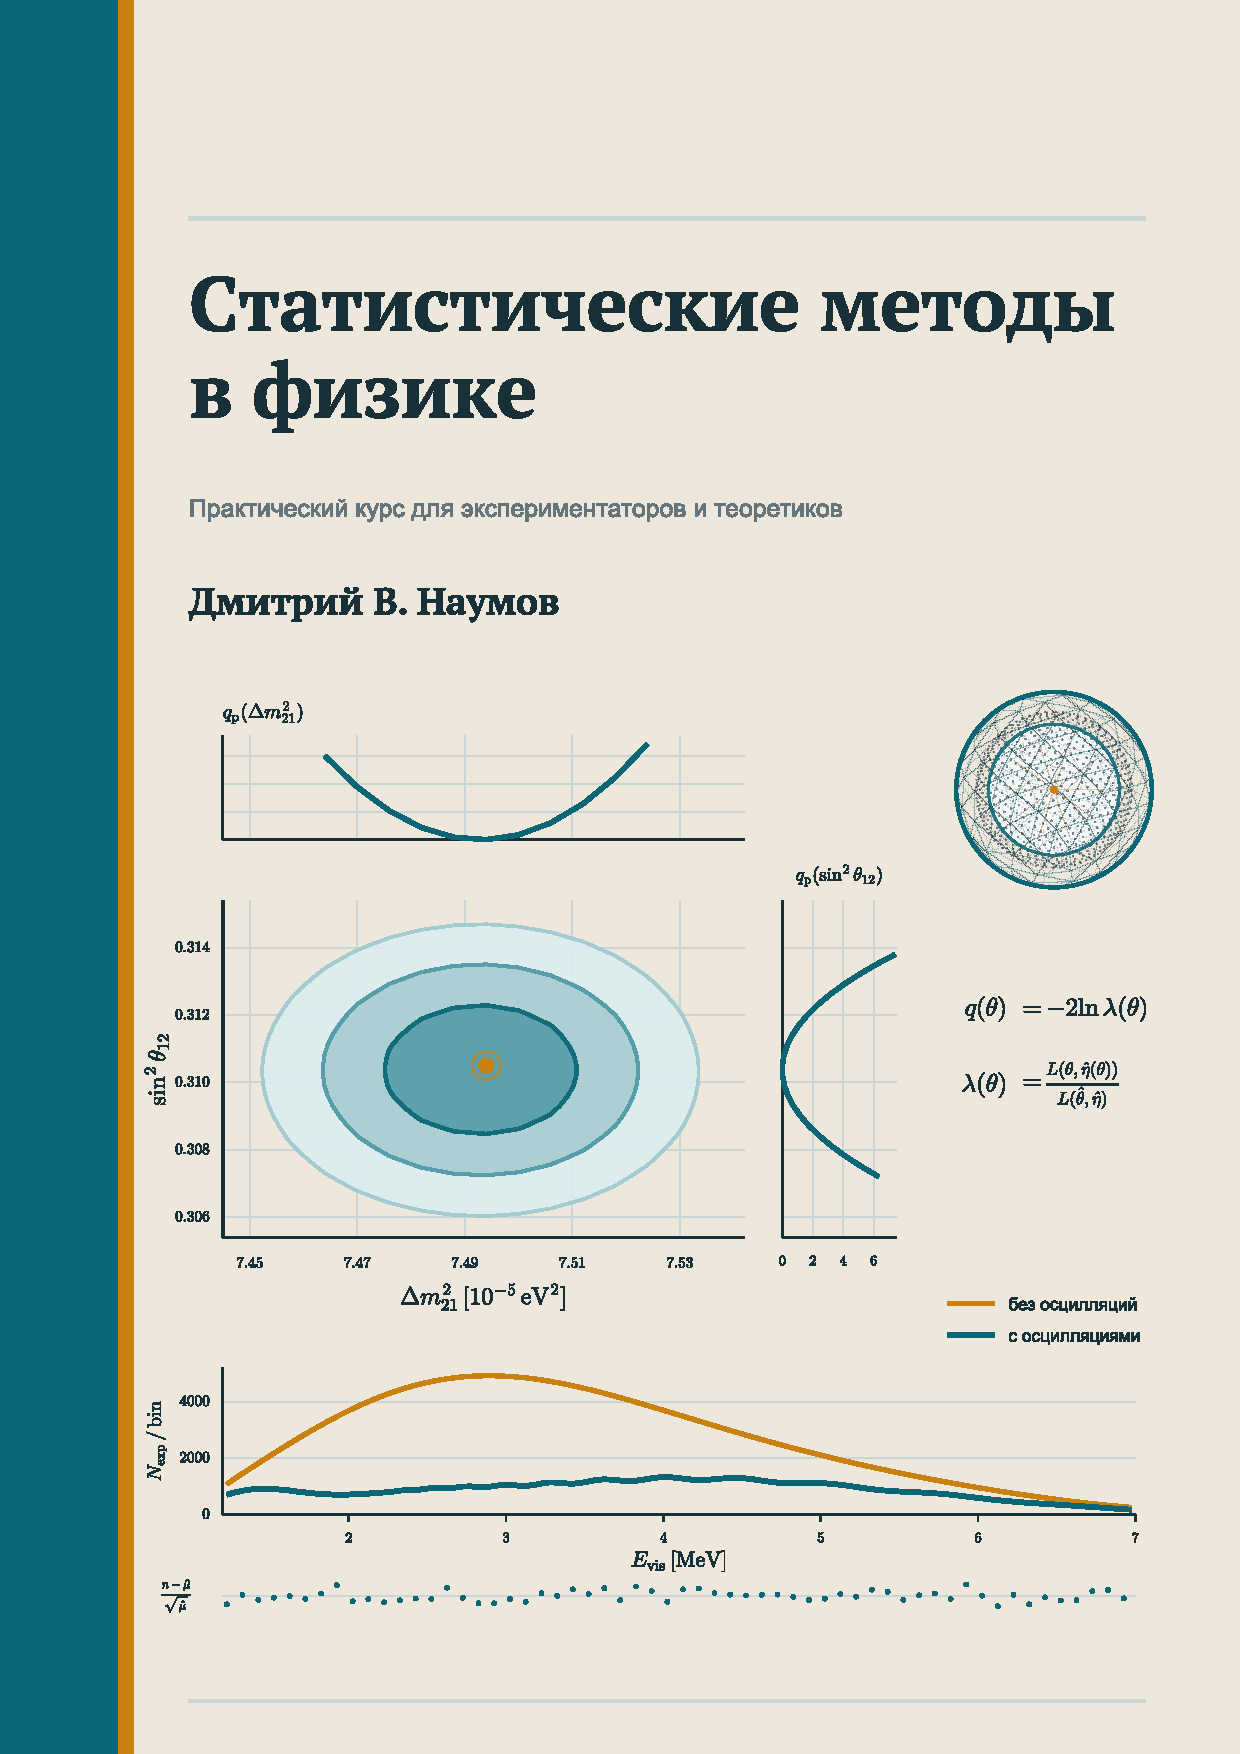
\includepdf[pages=1,fitpaper=true,pagecommand={\thispagestyle{empty}}]{assets/covers/front.pdf}%
  \endgroup
  % Count the cover in the front matter so physical and printed parity agree.
  \hypersetup{pageanchor=true}%
}
\newcommand{\NeutrinoHitBackCover}{%
  \clearpage
  \begingroup
  \ifdefined\bookpagenavigatorfalse\bookpagenavigatorfalse\fi
  
\includepdf[pages=1,fitpaper=true,pagecommand={\thispagestyle{empty}\hypertarget{neutrinohit-back-cover}{}}]{assets/covers/back.pdf}%
  \endgroup
}
% Replace the previous title artwork while retaining its single printed TOC.
\AtBeginDocument{%
  \renewcommand{\maketitle}{%
    \NeutrinoHitFrontCover
    \tableofcontents
    \clearpage
  }%
}
\usepackage{fontspec}
\usepackage{polyglossia}
\usepackage{unicode-math}
\usepackage{amsmath}
\usepackage{mathtools}
\usepackage{graphicx}
\usepackage{float}
\usepackage{booktabs}
\usepackage{longtable}
\usepackage{array}
\usepackage{microtype}
\usepackage{hyperref}

\defaultfontfeatures{Ligatures=TeX, Scale=MatchLowercase}
\setmainfont{Libertinus Serif}
\setsansfont{Libertinus Sans}
\setmonofont{Libertinus Mono}[Scale=0.9]
\setmathfont{Libertinus Math}

\setlength{\emergencystretch}{3em}

\hypersetup{
  pdfborder={0 0 0},
  colorlinks=true,
  linkcolor=black,
  citecolor=black,
  urlcolor=black
}

\newcommand{\E}{\mathbb{E}}
\newcommand{\Var}{\operatorname{Var}}
\newcommand{\cov}{\operatorname{cov}}
\newcommand{\dd}{\,\mathrm{d}}
\makeatletter
\@ifpackageloaded{bookmark}{}{\usepackage{bookmark}}
\makeatother
\makeatletter
\@ifpackageloaded{caption}{}{\usepackage{caption}}
\AtBeginDocument{%
\ifdefined\contentsname
  \renewcommand*\contentsname{Содержание}
\else
  \newcommand\contentsname{Содержание}
\fi
\ifdefined\listfigurename
  \renewcommand*\listfigurename{Список Иллюстраций}
\else
  \newcommand\listfigurename{Список Иллюстраций}
\fi
\ifdefined\listtablename
  \renewcommand*\listtablename{Список Таблиц}
\else
  \newcommand\listtablename{Список Таблиц}
\fi
\ifdefined\figurename
  \renewcommand*\figurename{Рисунок}
\else
  \newcommand\figurename{Рисунок}
\fi
\ifdefined\tablename
  \renewcommand*\tablename{Таблица}
\else
  \newcommand\tablename{Таблица}
\fi
}
\@ifpackageloaded{float}{}{\usepackage{float}}
\floatstyle{ruled}
\@ifundefined{c@chapter}{\newfloat{codelisting}{h}{lop}}{\newfloat{codelisting}{h}{lop}[chapter]}
\floatname{codelisting}{Список}
\newcommand*\listoflistings{\listof{codelisting}{Список Каталогов}}
\makeatother
\makeatletter
\makeatother
\makeatletter
\@ifpackageloaded{caption}{}{\usepackage{caption}}
\@ifpackageloaded{subcaption}{}{\usepackage{subcaption}}
\makeatother
\usepackage{bookmark}
\IfFileExists{xurl.sty}{\usepackage{xurl}}{} % add URL line breaks if available
\urlstyle{same}
\hypersetup{
  pdftitle={Статистический анализ данных},
  pdfauthor={Дмитрий В. Наумов},
  pdflang={ru},
  colorlinks=true,
  linkcolor={Maroon},
  filecolor={Maroon},
  citecolor={Blue},
  urlcolor={Blue},
  pdfcreator={LaTeX via pandoc}}


\title{Статистический анализ данных}
\usepackage{etoolbox}
\makeatletter
\providecommand{\subtitle}[1]{% add subtitle to \maketitle
  \apptocmd{\@title}{\par {\large #1 \par}}{}{}
}
\makeatother
\subtitle{От вероятности к физическому результату}
\author{Дмитрий В. Наумов}
\date{}
\begin{document}
\frontmatter
\maketitle


\mainmatter
Книга посвящена статистическим методам, которые используются при анализе
экспериментальных данных: от вероятностной модели и оценки параметров до
проверки гипотез и формулировки физического результата.

\bookmarksetup{startatroot}

\chapter*{Предисловие}\label{ux43fux440ux435ux434ux438ux441ux43bux43eux432ux438ux435}
\addcontentsline{toc}{chapter}{Предисловие}

\markboth{Предисловие}{Предисловие}

Статистическая процедура входит в определение экспериментального
результата. Выбор функции правдоподобия, учёт фона и систематических
неопределённостей, построение доверительных интервалов и проверка
гипотез определяют, какой физический вывод можно сделать по данным.

Книга выросла из курса по методам статистического анализа, которыми
приходится пользоваться в экспериментальной физике. Материал отобран по
опыту трёх десятилетий работы с данными в физике элементарных частиц,
нейтринной физике и астрофизике.

Теоретическое изложение сопровождается физическими примерами,
вычислениями, кодом на Python и интерактивными приложениями. Их можно
использовать для проверки формул и для самостоятельного анализа простых
моделей.

Для каждого метода обсуждаются статистическая модель, условия
применимости и смысл полученного результата. Отдельное внимание уделено
ошибкам, которые возникают при выборе модели, оценке параметров и
интерпретации статистического вывода.

Курс создан в рамках программы «Физика нейтрино и астрофизика частиц».
Он рассчитан на студентов старших курсов, аспирантов и исследователей,
знакомых с основами теории вероятностей, математического анализа и
программирования на Python.

\part{I. Вероятностный язык}

\chapter{Зачем физику
статистика}\label{ux437ux430ux447ux435ux43c-ux444ux438ux437ux438ux43aux443-ux441ux442ux430ux442ux438ux441ux442ux438ux43aux430}

\bookchapteropeningcontents

\begin{bookchapteropening}[Аннотация]

В этой главе объясняется, зачем физику нужен статистический анализ. На
примерах из реальных научных статей мы познакомимся с первыми
статистическими понятиями и проследим путь от теоретического расчёта и
экспериментальных данных к физическому выводу.

Введём основные обозначения, обсудим частотную и байесовскую
интерпретации вероятности --- два принципиально разных взгляда на
статистический вывод. Поговорим также о том, почему некоторые решения об
анализе нужно принимать ещё до того, как исследователь увидел результат.
Наконец, выполним первую подгонку по псевдоданным.

\end{bookchapteropening}

\section{О чём этот
курс?}\label{ux43e-ux447ux451ux43c-ux44dux442ux43eux442-ux43aux443ux440ux441}

В этом курсе мы разберём основные понятия, методы и язык, на котором
физики обсуждают результаты эксперимента. Прочитайте несколько обычных
фраз из научных статей:

\begin{itemize}
\tightlist
\item
  «Обнаружен сигнал со значимостью \(5\sigma\).»
\item
  «Наблюдается значимый избыток событий.»
\item
  «Область параметров исключена на уровне 95\% C.L.»
\item
  «Установлен верхний предел на сечение.»
\item
  «Фит сошёлся.»
\item
  «Доминирует систематическая неопределённость.»
\item
  «Корреляции между бинами существенны.»
\item
  «Мешающие параметры профилированы.»
\item
  «Использована полная ковариационная матрица.»
\end{itemize}

Всё ли здесь понятно? Если нет, этот курс может оказаться полезным.

\section{Четыре шага в научном
исследовании}\label{ux447ux435ux442ux44bux440ux435-ux448ux430ux433ux430-ux432-ux43dux430ux443ux447ux43dux43eux43c-ux438ux441ux441ux43bux435ux434ux43eux432ux430ux43dux438ux438}

Зачем вообще физику статистика? Рассмотрим типичный путь
экспериментального исследования.

\begin{enumerate}
\def\labelenumi{\arabic{enumi}.}
\item
  \textbf{Теория и физическая модель.} Теория описывает физический
  процесс и позволяет вычислить наблюдаемые величины. Например, число и
  распределение по кинематическим переменным бозонов Хиггса, которые
  должны рождаться на БАК при заданных параметрах модели.
\item
  \textbf{Эксперимент.} Детектор регистрирует события и после
  реконструкции и отбора даёт конкретный набор данных
  \(\mathbf d_{\mathrm{obs}}\).
\item
  \textbf{Статистический анализ.} Данные \(\mathbf d_{\mathrm{obs}}\)
  сопоставляются с моделью. По ним оцениваются параметры, проверяются
  гипотезы и определяется статистическая неопределённость сделанного
  вывода.
\item
  \textbf{Физический результат.} Результат анализа формулируется как
  измерение параметров, наблюдение или открытие эффекта, исключение
  области параметров либо верхний предел. После этого он становится
  результатом научной статьи.
\end{enumerate}

\begin{booknote}

Статистический анализ связывает теоретический расчёт с физическим
выводом из данных. Без него невозможно количественно ответить на главный
вопрос эксперимента: насколько наблюдаемый результат согласуется с той
или иной физической моделью?

Заявления ветхозаветных старцев о том, что они всё видят на глазок и
статистический анализ им не нужен, в современной экспериментальной
физике имеют весьма ограниченную область применимости.

\end{booknote}

\section{Обозначения}\label{ux43eux431ux43eux437ux43dux430ux447ux435ux43dux438ux44f}

В этой книге и онлайн-курсе будем использовать следующие обозначения.

\begin{itemize}
\tightlist
\item
  Скалярные величины обозначаются курсивом: \(x\), \(y\), \(\theta\).
\item
  Векторы --- полужирным шрифтом: \[
  \mathbf{x}=(x_1,x_2,\dots,x_n).
  \]
\item
  Матрицы --- полужирными заглавными буквами: \(\mathbf V\),
  \(\mathbf M\).
\item
  Случайные величины обозначаются заглавными буквами: \(X\), \(Y\);
  случайные векторы --- \(\mathbf X\), \(\mathbf D\).
\item
  Их конкретные наблюдаемые значения обозначаются строчными буквами:
  \(x\), \(y\), \(\mathbf d_{\mathrm{obs}}\).
\item
  Вероятность события \(A\) обозначается \(P(A)\).
\item
  Вероятность для дискретной величины или плотность вероятности для
  непрерывной будем обозначать \(p(x)\) или \(f(x)\).
\item
  Параметр модели обозначается \(\theta\), а набор параметров ---
  \(\boldsymbol{\theta}\).
\item
  Оценка параметра, вычисленная по данным, обозначается
  \(\widehat{\theta}\) или \(\widehat{\boldsymbol{\theta}}\).
\item
  Математическое ожидание: \(\mathbb E[X]\).
\item
  Дисперсия: \(\operatorname{Var}(X)\).
\item
  Стандартное отклонение: \[
  \sigma_X=\sqrt{\operatorname{Var}(X)}.
  \]
\item
  Ковариация: \(\operatorname{cov}(X,Y)\).
\item
  Коэффициент корреляции: \(\rho(X,Y)\).
\end{itemize}

\section{Что предсказывает
теория?}\label{ux447ux442ux43e-ux43fux440ux435ux434ux441ux43aux430ux437ux44bux432ux430ux435ux442-ux442ux435ux43eux440ux438ux44f}

Слово «предсказывает» звучит несколько странно --- будто теория
представляет собой дельфийского оракула. Это калька с английского
\emph{predict}, давно вошедшая в язык физиков. Имеется в виду просто
результат вычисления.

Теория может предсказывать сечение процесса, спектр энергии частиц,
вероятность распада или другую физическую величину. Но эксперимент
наблюдает не непосредственно эти величины, а отклик реальной установки.
Поэтому для статистического анализа нужна более полная модель,
включающая физическое предсказание, фон, отклик детектора, эффективность
регистрации и другие существенные детали эксперимента.

В результате мы приходим к вероятностной модели возможных данных: \[
p(\mathbf d\mid\boldsymbol{\theta}),
\] где \(\mathbf d\) обозначает возможный результат эксперимента, а
\(\boldsymbol{\theta}\) --- параметры модели.

Эта запись отвечает на вопрос:

\begin{quote}
если параметры равны \(\boldsymbol{\theta}\), какие данные \(\mathbf d\)
и с какой вероятностью может получить эксперимент?
\end{quote}

Для дискретных данных \(p(\mathbf d\mid\boldsymbol{\theta})\) означает
вероятность, для непрерывных --- плотность вероятности.

\section{Что наблюдает
эксперимент?}\label{ux447ux442ux43e-ux43dux430ux431ux43bux44eux434ux430ux435ux442-ux44dux43aux441ux43fux435ux440ux438ux43cux435ux43dux442}

До проведения эксперимента будущие данные неизвестны. Их будем описывать
случайным вектором \(\mathbf D\) с распределением \[
p(\mathbf d\mid\boldsymbol{\theta}).
\]

Коротко это будем записывать как \[
\mathbf D\sim p(\mathbf d\mid\boldsymbol{\theta}).
\]

Знак \(\sim\) здесь означает «распределён согласно».

После проведения эксперимента получен один конкретный результат: \[
\mathbf d_{\mathrm{obs}}.
\]

Таким образом, \(\mathbf D\) --- случайный результат ещё не проведённого
или мысленно повторяемого эксперимента, а \(\mathbf d_{\mathrm{obs}}\)
--- уже наблюдаемые данные.

Под символом \(\mathbf d\) может скрываться что угодно: число событий,
набор измеренных энергий, гистограмма, времена регистрации или весь
набор данных эксперимента.

\section{Суть статистического анализа в двух
словах}\label{ux441ux443ux442ux44c-ux441ux442ux430ux442ux438ux441ux442ux438ux447ux435ux441ux43aux43eux433ux43e-ux430ux43dux430ux43bux438ux437ux430-ux432-ux434ux432ux443ux445-ux441ux43bux43eux432ux430ux445}

Итак, у нас есть наблюдаемые данные \[
\mathbf d_{\mathrm{obs}}
\] и статистическая модель \[
p(\mathbf d\mid\boldsymbol{\theta}).
\]

Дальше возникают два основных типа вопросов.

\begin{enumerate}
\def\labelenumi{\arabic{enumi}.}
\item
  \textbf{Оценивание параметров.} Какие значения параметров
  \(\boldsymbol{\theta}\) лучше всего согласуются с полученными данными?
  Результатом является оценка \[
  \widehat{\boldsymbol{\theta}}
  \] и её неопределённость.
\item
  \textbf{Проверка гипотез.} Насколько данные согласуются с определённой
  гипотезой? Например, совместимы ли они с отсутствием сигнала, можно ли
  исключить некоторую область параметров или достаточно ли велико
  наблюдаемое отклонение, чтобы говорить об открытии?
\end{enumerate}

Обе задачи начинаются с одной и той же вероятностной модели \[
p(\mathbf d\mid\boldsymbol{\theta}),
\] но отвечают на разные вопросы.

В этом курсе мы научимся формулировать эти вопросы точно и строить
статистические процедуры, которые позволяют на них отвечать.

\section{Два взгляда на
вероятность}\label{ux434ux432ux430-ux432ux437ux433ux43bux44fux434ux430-ux43dux430-ux432ux435ux440ux43eux44fux442ux43dux43eux441ux442ux44c}

Если вам случится оказаться на большой конференции по статистике, вы
быстро обнаружите представителей двух школ: частотной и байесовской.

Они используют одну и ту же теорему вероятностей, но по-разному
понимают, к каким объектам вообще допустимо применять слово
«вероятность».

\subsection{Частотная
вероятность}\label{ux447ux430ux441ux442ux43eux442ux43dux430ux44f-ux432ux435ux440ux43eux44fux442ux43dux43eux441ux442ux44c}

В частотном подходе вероятность связывают с относительной частотой
события \(A\) в серии одинаковых опытов:

\begin{equation}\protect\phantomsection\label{eq-frequency-probability}{
P(A)=\lim_{n\to\infty}
\frac{\text{число наблюдений события }A}{n}.
}\end{equation}

Это операциональная интерпретация вероятности. Параметры модели
считаются фиксированными, хотя их значения могут быть неизвестны. При
повторении эксперимента меняются данные.

Например, если истинная масса частицы равна \(m\), то при многократном
повторении измерения будут меняться результаты эксперимента и
построенные по ним оценки \(\widehat m\), но сама масса \(m\) в этой
постановке не флуктуирует.

\subsection{Байесовская
вероятность}\label{ux431ux430ux439ux435ux441ux43eux432ux441ux43aux430ux44f-ux432ux435ux440ux43eux44fux442ux43dux43eux441ux442ux44c}

Теорема Байеса для параметров модели записывается в виде

\begin{equation}\protect\phantomsection\label{eq-bayes-theorem}{
p(\boldsymbol{\theta}\mid\mathbf d)
=
\frac{
p(\mathbf d\mid\boldsymbol{\theta})\,
\pi(\boldsymbol{\theta})
}{
p(\mathbf d)
}.
}\end{equation}

Здесь

\begin{itemize}
\tightlist
\item
  \(p(\mathbf d\mid\boldsymbol{\theta})\) --- вероятность или плотность
  данных при фиксированных параметрах модели;
\item
  \(\pi(\boldsymbol{\theta})\) --- априорное распределение параметров;
\item
  \(p(\boldsymbol{\theta}\mid\mathbf d)\) --- апостериорное
  распределение после получения данных;
\item
  \(p(\mathbf d)\) --- нормировочный множитель,
\end{itemize}

\[
p(\mathbf d)
=
\int
p(\mathbf d\mid\boldsymbol{\theta})
\pi(\boldsymbol{\theta})\,d\boldsymbol{\theta}.
\]

\begin{semanticpdfbox}[colback=BookBiographySoft,borderline west={1.2mm}{0pt}{BookBiography},breakable=false]

\noindent\begin{minipage}[t]{30mm}\vspace{0pt}\centering

\href{https://mathshistory.st-andrews.ac.uk/Biographies/Bayes/pictdisplay/}{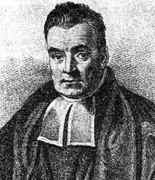
\includegraphics[width=28mm,height=\textheight,keepaspectratio,alt={Портрет, традиционно связываемый с Томасом Байесом}]{assets/people/thomas-bayes.jpg}}

\end{minipage}\hfill\begin{minipage}[t]{\dimexpr\linewidth-35mm\relax}\vspace{0pt}

{\sffamily\bfseries\footnotesize\color{BookBiography} БИОГРАФИЯ\par}\vspace{0.8mm}{\sffamily\bfseries\large\color{BookInk} Томас Байес\par}

{\sffamily\small\color{BookMuted} 1701–1761\par}\vspace{1.4mm}

Томас Байес --- английский пресвитер и математик. Его работу об обратной
вероятности опубликовали после смерти автора. Формула, получившая имя
Байеса, связывает условные вероятности и лежит в основе байесовского
вывода.

{\footnotesize\color{BookMuted}

\textbf{Источник:}
\href{https://mathshistory.st-andrews.ac.uk/Biographies/Bayes/}{MacTutor};
фото
\href{https://mathshistory.st-andrews.ac.uk/Biographies/Bayes/pictdisplay/}{MacTutor}

}

\end{minipage}

\end{semanticpdfbox}

\begin{figure}[H]

\centering{

\pandocbounded{
\includegraphics[keepaspectratio]{index_files/mediabag/chapters/../assets/figures/bayes-theorem.pdf}}

}

\caption{\label{fig-bayes-theorem}Визуальное доказательство теоремы
Байеса}

\end{figure}%

На рисунке \ref{fig-bayes-theorem} обе части равенства

\[
P(A\mid B)P(B)=P(B\mid A)P(A)
\]

соответствуют одной и той же области пересечения \(A\cap B\).

Сама формула возражений не вызывает. Вопрос начинается с множителя
\(\pi(\boldsymbol{\theta})\). Откуда известно распределение параметра до
измерения?

У \(p(\mathbf d\mid\boldsymbol{\theta})\) вполне прозрачный смысл.
Фиксируем \(\boldsymbol{\theta}\), многократно повторяем эксперимент и
смотрим, как распределены данные \(\mathbf d\). Именно такой опыт
определяет вероятность в частотной постановке.

Попробуем тем же способом понять \(\pi(\boldsymbol{\theta})\). Возьмём
массу электрона. Чтобы буквально прочитать \(\pi(m_e)\) как частоту,
пришлось бы рассмотреть бесконечное число Вселенных с разными массами
электрона и узнать, как эти массы распределены. В нашем распоряжении
одна Вселенная и одна масса электрона. Никакой серии опытов, в которой
природа каждый раз заново выбирает \(m_e\), у нас нет.

В байесовской интерпретации \(\pi(\boldsymbol{\theta})\) описывает
степень знания о параметре, а не частоту его появления в разных
Вселенных. Здесь и начинается спор. Слово «вероятность» применяется к
двум разным объектам. В \(p(\mathbf d\mid\boldsymbol{\theta})\)
случайность относится к результату повторяемого эксперимента. В
\(\pi(\boldsymbol{\theta})\) она относится к нашему незнанию
фиксированного параметра.

Последовательное байесовское обновление частично снимает эту проблему.
Пусть сначала получены данные \(\mathbf d_1\). Построенное по ним
распределение \(p(\boldsymbol{\theta}\mid\mathbf d_1)\) можно
использовать как априорное при анализе следующего независимого измерения
\(\mathbf d_2\):

\begin{equation}\protect\phantomsection\label{eq-bayes-sequential-update}{
p(\boldsymbol{\theta}\mid\mathbf d_1,\mathbf d_2)
\propto
p(\mathbf d_2\mid\boldsymbol{\theta})
p(\boldsymbol{\theta}\mid\mathbf d_1).
}\end{equation}

Апостериорное распределение первого эксперимента становится априорным
для второго. Такое последовательное обновление однозначно определено, но
вопрос о самом первом \(\pi_0(\boldsymbol{\theta})\) остаётся.

Рассмотрим простейшее измерение
\(x\mid\theta\sim\mathcal N(\theta,s^2)\). Если на существенном для
функции правдоподобия интервале взять плоское априорное распределение,
то после одного измерения

\begin{equation}\protect\phantomsection\label{eq-bayes-flat-prior}{
p(\theta\mid x)
\propto
\exp\!\left[-\frac{(x-\theta)^2}{2s^2}\right].
}\end{equation}

После нормировки апостериорное распределение имеет ту же форму, что и
функция правдоподобия. Плоское распределение можно получить как предел
гауссова априорного распределения с очень большой шириной.

Теперь зададим другое начальное распределение \(\pi_0(\theta)\). Для
\(n\) независимых гауссовских измерений с одинаковой ошибкой \(s\)
получим

\begin{equation}\protect\phantomsection\label{eq-bayes-prior-memory}{
p(\theta\mid x_1,\ldots,x_n)
\propto
\pi_0(\theta)
\exp\!\left[-\frac{n(\theta-\bar x)^2}{2s^2}\right].
}\end{equation}

В уравнении \ref{eq-bayes-prior-memory} след первого выбора виден явно:
\(\pi_0(\theta)\) остаётся множителем при любом числе измерений. Когда
функция правдоподобия становится узкой, а априорное распределение почти
не меняется в этой узкой области, его влияние ослабевает. Если данных
мало, априорное распределение быстро меняется в интересующей области или
вообще запрещает часть значений параметра, след начального выбора
сохраняется.

Тем не менее, байесовский подход имеет своих сторонников и он
используется в большом числе физических анализов. Одним из важных
практических преимуществ этого метода является более высокая скорость
получения результата в задачах с большим числом параметров. После
построения выборки из совместного апостериорного распределения
маргинальные распределения отдельных параметров получаются простым
суммированием по этой выборке. Для построения частотного профиля
приходится при каждом значении интересующего параметра заново искать
максимум по мешающим параметрам. Если параметров много и требуется
несколько проекций, разница во времени может быть существенной.

Универсального выигрыша здесь нет. Получение многомерной апостериорной
выборки само может оказаться сложнее серии минимизаций. Вычислительное
удобство зависит от модели и алгоритма и ничего не говорит о физическом
смысле \(\pi(\boldsymbol{\theta})\).

Мне ближе частотная постановка. Основная часть книги и курса строится
именно в таком подходе. Байесовский подход мы тоже разберём: читатель
должен видеть исходное предположение и понимать, где оно вошло в
результат.

\subsection{Два разных
интервала}\label{ux434ux432ux430-ux440ux430ux437ux43dux44bux445-ux438ux43dux442ux435ux440ux432ux430ux43bux430}

Различие между частотным и байесовским подходами особенно хорошо видно
на примере того, что в разговорной речи часто называют «интервалом
ошибок».

Предположим, после измерения мы получили некоторый интервал для
неизвестного параметра \(\theta\). Что означает число 95\%?

\textbf{Частотный подход} отвечает на вопрос:

\begin{quote}
Если много раз повторить эксперимент и каждый раз заново построить
интервал, какая доля этих интервалов накроет истинное значение
\(\theta\)?
\end{quote}

95\%-й доверительный интервал --- это процедура \(C(\mathbf D)\), для
которой

\begin{equation}\protect\phantomsection\label{eq-frequentist-coverage}{
P_\theta\!\left(\theta\in C(\mathbf D)\right)=0.95.
}\end{equation}

Случайным здесь является интервал: от эксперимента к эксперименту
меняются данные \(\mathbf D\) и построенные по ним границы. Параметр
\(\theta\) считается фиксированным.

После того как эксперимент уже выполнен и конкретный интервал получен,
частотный подход не приписывает вероятности утверждению «\(\theta\)
находится внутри этого интервала».

\textbf{Байесовский подход} отвечает на другой вопрос:

\begin{quote}
После получения этих данных как распределена наша неопределённость
относительно самого параметра \(\theta\)?
\end{quote}

95\%-й байесовский интервал \(C_B(\mathbf d)\) содержит 95\%
апостериорной вероятности:

\begin{equation}\protect\phantomsection\label{eq-bayesian-credible-interval}{
\int_{C_B(\mathbf d)}
p(\theta\mid\mathbf d)\,d\theta
=0.95.
}\end{equation}

Здесь уже можно сказать: при заданной модели и выбранном априорном
распределении апостериорная вероятность того, что \(\theta\) лежит в
этом интервале, равна 95\%.

Таким образом, одинаковое число 95\% отвечает на два разных вопроса:

\begin{itemize}
\tightlist
\item
  в частотном подходе --- \textbf{как ведёт себя процедура при
  повторении эксперимента?}
\item
  в байесовском --- \textbf{что мы знаем о параметре после получения
  данных?}
\end{itemize}

Границы этих интервалов иногда оказываются близкими или даже совпадают.
Их статистический смысл от этого не становится одинаковым.

\section{Как выглядят открытия и
исключения}\label{ux43aux430ux43a-ux432ux44bux433ux43bux44fux434ux44fux442-ux43eux442ux43aux440ux44bux442ux438ux44f-ux438-ux438ux441ux43aux43bux44eux447ux435ux43dux438ux44f}

Теперь посмотрим на несколько реальных результатов из экспериментальной
физики.

На первый взгляд это просто графики. Но именно из таких графиков физики
делают выводы об открытии новых частиц, измерении параметров и
исключении целых областей теории.

Попробуйте понять, что именно на них изображено и почему из этих данных
следуют такие сильные утверждения.

\subsection{Открытие бозона
Хиггса}\label{ux43eux442ux43aux440ux44bux442ux438ux435-ux431ux43eux437ux43eux43dux430-ux445ux438ux433ux433ux441ux430}

На рисунках \ref{fig-atlas-higgs-pvalue} и \ref{fig-cms-higgs-pvalue}
показаны результаты поисков бозона Хиггса в экспериментах ATLAS и CMS.

Перед чтением подписей попробуйте ответить:

\begin{itemize}
\tightlist
\item
  Что отложено по вертикальной оси?
\item
  Что такое \(p\)-значение?
\item
  Почему минимум кривой указывает на возможный сигнал?
\item
  Что означают линии \(1\sigma\), \(2\sigma\), \ldots, \(5\sigma\)?
\item
  Почему достижение \(5\sigma\) позволило говорить об открытии?
\item
  Почему различают локальную и глобальную значимость?
\end{itemize}

\begin{figure}[H]

\centering{

\pandocbounded{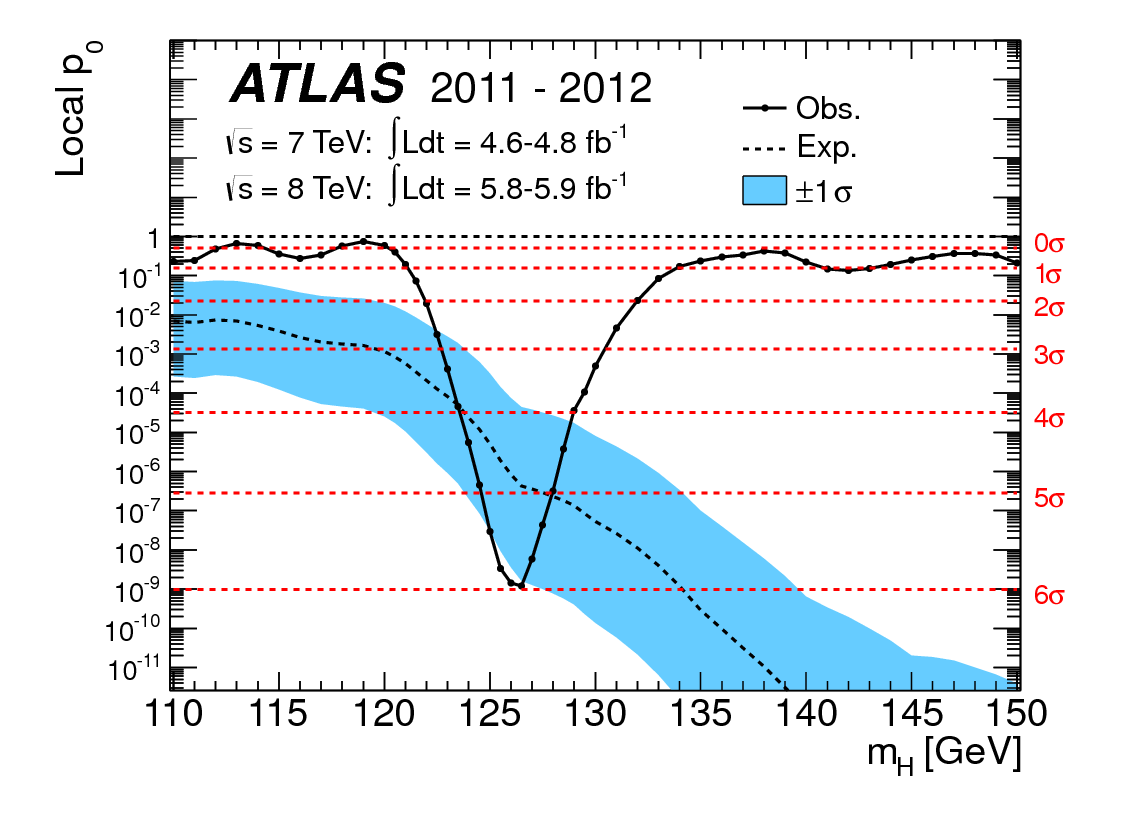
\includegraphics[keepaspectratio]{chapters/../assets/figures/Atlas_pvalue.png}}

}

\caption{\label{fig-atlas-higgs-pvalue}Локальное \(p\)-значение фоновой
гипотезы в результате ATLAS}

\end{figure}%

\begin{figure}[H]

\centering{

\pandocbounded{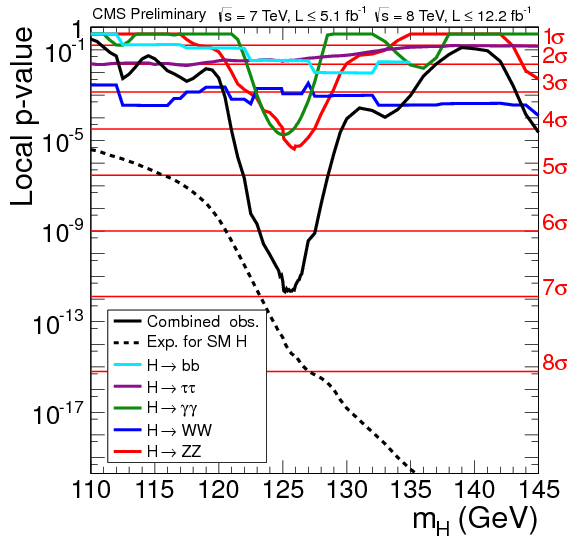
\includegraphics[keepaspectratio]{chapters/../assets/figures/CMS_pvalue.png}}

}

\caption{\label{fig-cms-higgs-pvalue}Локальное \(p\)-значение фоновой
гипотезы в результате CMS}

\end{figure}%

По горизонтали перебирается предполагаемая масса бозона Хиггса. Чёрные
кривые получены из экспериментальных данных. В районе
\(125\,\text{ГэВ}\) оба эксперимента наблюдают особенно сильное
отклонение от фоновой гипотезы.

ATLAS сообщил локальную значимость \(5.9\sigma\), CMS --- \(5.0\sigma\)
{[}1, 2{]}.

Почему именно эти числа означают открытие, мы разберём дальше.

Нобелевскую премию по физике 2013 года получили Франсуа Энглер и Питер
Хиггс за теоретическое открытие механизма происхождения массы
элементарных частиц. В формулировке Нобелевского комитета его
экспериментальное подтверждение связано с открытием новой частицы
экспериментами ATLAS и CMS {[}3{]}.

\subsection{Измерение параметра в Daya
Bay}\label{ux438ux437ux43cux435ux440ux435ux43dux438ux435-ux43fux430ux440ux430ux43cux435ux442ux440ux430-ux432-daya-bay}

Другой тип результата показан на рисунке \ref{fig-daya-bay-theta13}.
Эксперимент Daya Bay измерял угол смешивания нейтрино \(\theta_{13}\).

Попробуйте ответить:

\begin{itemize}
\tightlist
\item
  Что означает красная кривая?
\item
  Что такое \emph{best fit}?
\item
  Почему минимум \(\chi^2\) определяет измеренное значение параметра?
\item
  Что именно означает значимость \(5.2\sigma\)?
\item
  Означает ли хороший \emph{best fit}, что теория доказана?
\end{itemize}

\begin{figure}[H]

\centering{

\pandocbounded{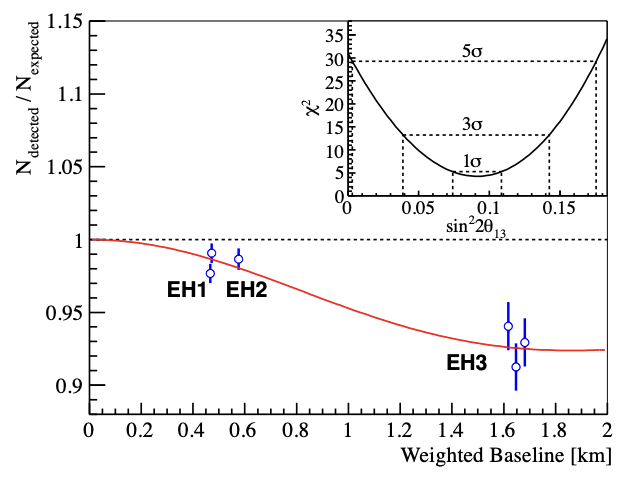
\includegraphics[keepaspectratio]{chapters/../assets/figures/DayaBayTheta13.png}}

}

\caption{\label{fig-daya-bay-theta13}Измерение ненулевого угла
смешивания \(\theta_{13}\) в Daya Bay}

\end{figure}%

Красная кривая показывает осцилляционное предсказание при значении
\(\sin^2 2\theta_{13}\), найденном из совместной подгонки данных. Во
вставке показана зависимость \(\chi^2\) от этого параметра.

Daya Bay отверг гипотезу \(\theta_{13}=0\) со значимостью \(5.2\sigma\)
{[}4{]}.

Почему минимум \(\chi^2\) даёт оценку параметра и откуда возникает
статистическая значимость, пока оставим без ответа.

\subsection{Исключение области
параметров}\label{ux438ux441ux43aux43bux44eux447ux435ux43dux438ux435-ux43eux431ux43bux430ux441ux442ux438-ux43fux430ux440ux430ux43cux435ux442ux440ux43eux432}

Наконец, посмотрим на результат поиска стерильных нейтрино в Daya Bay.

\begin{figure}[H]

\centering{

\pandocbounded{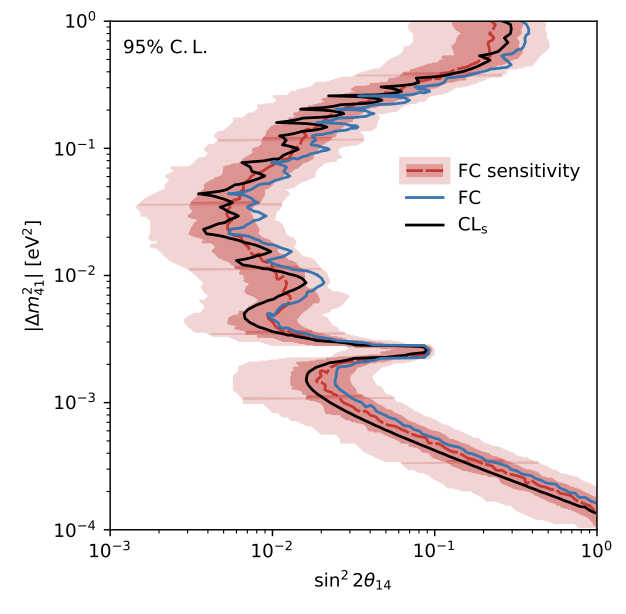
\includegraphics[keepaspectratio]{chapters/../assets/figures/DBSterile.png}}

}

\caption{\label{fig-daya-bay-sterile-exclusion}Исключение области
параметров стерильных нейтрино в Daya Bay}

\end{figure}%

Здесь уже нет одного измеренного числа. Результат представлен областью
на плоскости параметров \[
\sin^2 2\theta_{14},
\qquad
|\Delta m^2_{41}|.
\]

Попробуйте понять:

\begin{itemize}
\tightlist
\item
  Что означает фраза «область исключена на уровне 95\%»?
\item
  Почему результатом является контур, а не одна точка?
\item
  Что означает \emph{sensitivity}?
\item
  Почему на одном графике показаны две разные статистические процедуры
  --- Feldman--Cousins и \(CL_s\)?
\item
  Почему их границы не обязаны совпадать?
\end{itemize}

Полный набор Daya Bay содержит \(5.55\cdot10^6\) кандидатов за 3158 дней
{[}5{]}.

К концу курса все элементы этих четырёх рисунков должны стать понятными.

\section{Первый фит: ширина
гауссианы}\label{ux43fux435ux440ux432ux44bux439-ux444ux438ux442-ux448ux438ux440ux438ux43dux430-ux433ux430ux443ux441ux441ux438ux430ux43dux44b}

Рассмотрим выборку из гауссова распределения с известным центром
\(x_0=0\) и неизвестной шириной \(\sigma\):

\begin{equation}\protect\phantomsection\label{eq-gaussian-width-model}{
f(x;\sigma)=
\frac{1}{\sqrt{2\pi}\sigma}
\exp\!\left(-\frac{x^2}{2\sigma^2}\right).
}\end{equation}

Сгенерируем \(N\) псевдособытий при некотором фиксированном значении
\(\sigma_{\mathrm{true}}\) и разобьём ось \(x\) на интервалы. Для
интервала \(i\) модель предсказывает среднее число событий

\[
\mu_i(\sigma)
=
N\int_{\text{бин }i} f(x;\sigma)\,dx,
\]

а в сгенерированной выборке наблюдается \(n_i\) событий.

Теперь нужно определить, какое значение \(\sigma\) лучше всего описывает
полученную гистограмму. Для этого используем пуассоновский девианс ---
статистику отношения правдоподобий:

\begin{equation}\protect\phantomsection\label{eq-poisson-deviance}{
\chi^2(\sigma)
=
2\sum_i
\left[
\mu_i(\sigma)-n_i
+n_i\ln\frac{n_i}{\mu_i(\sigma)}
\right].
}\end{equation}

Для пустого интервала, \(n_i=0\), последнее слагаемое по пределу равно
нулю.

Чем меньше \(\chi^2(\sigma)\), тем лучше модель при данном \(\sigma\)
согласуется с выборкой. Значение в точке минимума определяет оценку

\[
\widehat{\sigma}
=
\arg\min_\sigma \chi^2(\sigma).
\]

\subsection{Интерактив: найдите ширину
распределения}\label{interactive-first-fit}

Сначала попробуйте подобрать \(\sigma\) на глаз по гистограмме. Затем
включите результат фита и сравните свою оценку с \(\widehat{\sigma}\) и
истинным значением \(\sigma_{\mathrm{true}}\).

\begin{semanticpdfbox}[breakable=false]

\begin{center}

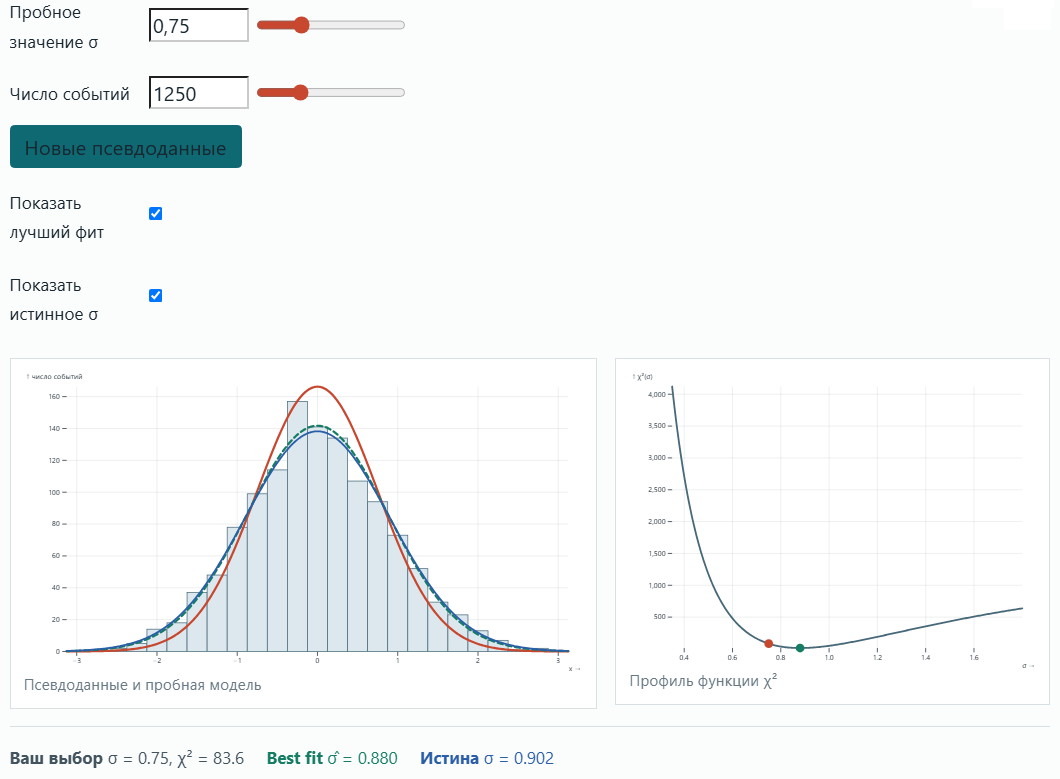
\includegraphics[width=0.74\linewidth,height=\textheight,keepaspectratio,alt={Подбор ширины распределения}]{assets/figures/distribution_width.png}

\end{center}

\noindent\begin{minipage}[c]{\dimexpr\linewidth-30mm\relax}

\textbf{Интерактив}. \textbf{Подбор ширины распределения}

Отсканируйте QR-код, чтобы открыть интерактив и самостоятельно подобрать
ширину распределения.

\end{minipage}\hfill\begin{minipage}[c]{26mm}\centering

\href{https://neutrinohit.github.io/statistical-analysis-course/ru/book/chapters/01_why_statistics.html\#interactive-first-fit}{
\includegraphics[width=24mm,height=\textheight,keepaspectratio,alt={QR-код интерактива}]{assets/qr/first_fit.png}}

\end{minipage}

\end{semanticpdfbox}

При новой генерации псевдоданных меняется положение минимума и,
следовательно, оценка \(\widehat{\sigma}\). Истинный параметр
\(\sigma_{\mathrm{true}}\) при этом остаётся тем же. С ростом числа
событий кривая \(\chi^2(\sigma)\) обычно становится уже: данные точнее
определяют ширину распределения.

\begin{bookchaptersummary}[Итоги главы]

\begin{itemize}
\item
  Статистическая модель \(p(\mathbf d\mid\boldsymbol{\theta})\) задаёт
  распределение возможных данных при фиксированных параметрах модели.
  Наблюдаемые данные \(\mathbf d_{\mathrm{obs}}\) --- одна конкретная
  реализация этого распределения.
\item
  В статистическом анализе возникают две разные задачи: оценивание
  параметров и проверка гипотез.
\item
  Параметр модели и его оценка --- разные объекты. При повторении
  эксперимента параметр остаётся фиксированным, а вычисленная по данным
  оценка \(\widehat{\boldsymbol{\theta}}\) меняется.
\item
  Частотный и байесовский подходы по-разному интерпретируют вероятность
  и статус неизвестных параметров. В байесовском выводе результат
  зависит также от выбранного априорного распределения.
\item
  Измерение параметра, открытие сигнала и исключение области параметров
  --- разные статистические выводы. Их смысл определяется не только
  данными, но также моделью и выбранной статистической процедурой.
\item
  Уже в простейшей подгонке видно, как из случайных данных возникает
  оценка параметра: истинная ширина \(\sigma_{\mathrm{true}}\)
  фиксирована, а найденное значение \(\widehat{\sigma}\) флуктуирует
  между выборками.
\end{itemize}

\end{bookchaptersummary}

\section{Задачи}\label{ux437ux430ux434ux430ux447ux438}

\begin{semanticpdfbox}[colback=BookCoralSoft,borderline west={1.2mm}{0pt}{BookCoral},breakable=false]

\noindent{\sffamily\bfseries\fontsize{11.2}{13.5}\selectfont Задача 1. Модель и данные}\par\nopagebreak[4]\vspace{1.2mm}

В некотором эксперименте теория предсказывает число событий

\[
\mathbf{t}=(10,\ 20,\ 10).
\]

Эксперимент дал результат

\[
\mathbf{d}=(12,\ 18,\ 11).
\]

Ответьте:

\begin{enumerate}
\def\labelenumi{\arabic{enumi}.}
\tightlist
\item
  Что здесь является предсказанием модели?
\item
  Что является данными эксперимента?
\item
  В каких бинах данные больше предсказания?
\item
  В каких бинах данные меньше предсказания?
\item
  Можно ли по этим числам сразу сказать, что теория неверна?
\end{enumerate}

\end{semanticpdfbox}

\begin{semanticpdfbox}[colback=BookCoralSoft,borderline west={1.2mm}{0pt}{BookCoral},breakable=false]

\noindent{\sffamily\bfseries\fontsize{11.2}{13.5}\selectfont Задача 2. Случайная величина и измеренное значение}\par\nopagebreak[4]\vspace{1.2mm}

До измерения результат эксперимента неизвестен. Обозначим его случайной
величиной \(X\).

После измерения получено значение

\[
x=7.3.
\]

Ответьте:

\begin{enumerate}
\def\labelenumi{\arabic{enumi}.}
\tightlist
\item
  Что обозначает \(X\)?
\item
  Что обозначает \(x\)?
\item
  Почему до измерения мы говорим о \(X\), а после измерения --- о \(x\)?
\item
  Приведите свой пример случайной величины и её измеренного значения.
\end{enumerate}

\end{semanticpdfbox}

\begin{semanticpdfbox}[colback=BookCoralSoft,borderline west={1.2mm}{0pt}{BookCoral},breakable=false]

\noindent{\sffamily\bfseries\fontsize{11.2}{13.5}\selectfont Задача 3. Частота как оценка вероятности}\par\nopagebreak[4]\vspace{1.2mm}

Детектор зарегистрировал 100 событий. Из них 23 события прошли отбор.

Ответьте:

\begin{enumerate}
\def\labelenumi{\arabic{enumi}.}
\tightlist
\item
  Какую долю событий отобрал алгоритм?
\item
  Как по этим данным оценить вероятность того, что следующее событие
  пройдёт отбор?
\item
  Будет ли эта оценка точно равна истинной вероятности?
\item
  Что изменится, если вместо 100 событий было бы зарегистрировано 10 000
  событий?
\end{enumerate}

\end{semanticpdfbox}

\begin{semanticpdfbox}[colback=BookCoralSoft,borderline west={1.2mm}{0pt}{BookCoral},breakable=false]

\noindent{\sffamily\bfseries\fontsize{11.2}{13.5}\selectfont Задача 4. Условная вероятность без формул}\par\nopagebreak[4]\vspace{1.2mm}

В выборке есть 1000 событий:

\begin{itemize}
\tightlist
\item
  100 сигнальных событий;
\item
  900 фоновых событий.
\end{itemize}

Алгоритм помечает событие как «интересное». Он пометил:

\begin{itemize}
\tightlist
\item
  80 сигнальных событий;
\item
  90 фоновых событий.
\end{itemize}

Ответьте:

\begin{enumerate}
\def\labelenumi{\arabic{enumi}.}
\tightlist
\item
  Сколько всего событий помечено как «интересные»?
\item
  Какая доля сигнальных событий была помечена?
\item
  Какая доля помеченных событий действительно является сигналом?
\item
  Почему это разные числа?
\item
  Что важнее для утверждения «мы нашли сигнал»: доля помеченных
  сигнальных событий или доля сигнала среди помеченных событий?
\end{enumerate}

\end{semanticpdfbox}

\begin{semanticpdfbox}[colback=BookCoralSoft,borderline west={1.2mm}{0pt}{BookCoral},breakable=false]

\noindent{\sffamily\bfseries\fontsize{11.2}{13.5}\selectfont Задача 5. Точка наилучшего согласия}\par\nopagebreak[4]\vspace{1.2mm}

Одна и та же форма кривой сравнивается с данными при разных значениях
параметра \(\sigma\).

Получены такие значения меры расхождения:

{\def\LTcaptype{none} % do not increment counter
\begin{longtable}[]{@{}rr@{}}
\toprule\noalign{}
\(\sigma\) & расхождение \\
\midrule\noalign{}
\endhead
\bottomrule\noalign{}
\endlastfoot
0.6 & 18.4 \\
0.8 & 7.2 \\
1.0 & 2.1 \\
1.2 & 3.5 \\
1.4 & 9.8 \\
\end{longtable}
}

Ответьте:

\begin{enumerate}
\def\labelenumi{\arabic{enumi}.}
\tightlist
\item
  При каком значении \(\sigma\) модель лучше всего согласуется с
  данными?
\item
  Почему это значение называется точкой наилучшего согласия?
\item
  Значит ли это, что истинное значение \(\sigma\) точно равно
  найденному?
\item
  Что нужно знать дополнительно, чтобы говорить об ошибке найденного
  значения?
\end{enumerate}

\end{semanticpdfbox}

\begin{semanticpdfbox}[colback=BookCoralSoft,borderline west={1.2mm}{0pt}{BookCoral},breakable=false]

\noindent{\sffamily\bfseries\fontsize{11.2}{13.5}\selectfont Задача 6. Флуктуация или систематический сдвиг?}\par\nopagebreak[4]\vspace{1.2mm}

Ожидаемое число событий в каждом запуске равно примерно 100.

В первом случае получены результаты:

\[
98,\quad 103,\quad 99,\quad 101,\quad 100.
\]

Во втором случае получены результаты:

\[
113,\quad 111,\quad 115,\quad 112,\quad 114.
\]

Ответьте:

\begin{enumerate}
\def\labelenumi{\arabic{enumi}.}
\tightlist
\item
  В каком случае данные выглядят как случайные флуктуации около 100?
\item
  В каком случае виден возможный систематический сдвиг?
\item
  Почему отдельное значение 103 не выглядит подозрительным?
\item
  Почему последовательность значений около 113 уже выглядит
  подозрительной?
\item
  Что следовало бы проверить в эксперименте во втором случае?
\end{enumerate}

\end{semanticpdfbox}

\begin{semanticpdfbox}[colback=BookCoralSoft,borderline west={1.2mm}{0pt}{BookCoral},breakable=false]

\noindent{\sffamily\bfseries\fontsize{11.2}{13.5}\selectfont Задача 7. Следы априорного распределения}\par\nopagebreak[4]\vspace{1.2mm}

Пусть измерения \(x_i\) независимы и имеют гауссовское распределение

\[
x_i\mid\theta\sim\mathcal N(\theta,1).
\]

Рассмотрите выборку со средним \(\bar x=1\) сначала при \(n=1\), а затем
при \(n=100\). Сравните три априорных распределения:

\[
\pi_1(\theta)\propto 1,
\qquad
\pi_2(\theta)\propto \exp\!\left(-\frac{\theta^2}{2}\right),
\qquad
\pi_3(\theta)\propto \frac{1}{1+\theta^2}.
\]

Для каждого случая постройте функцию

\[
p(\theta\mid x_1,\ldots,x_n)
\propto
\pi_k(\theta)
\exp\!\left[-\frac{n(\theta-\bar x)^2}{2}\right].
\]

Ответьте:

\begin{enumerate}
\def\labelenumi{\arabic{enumi}.}
\tightlist
\item
  Насколько различаются три результата после одного измерения?
\item
  Что меняется после ста измерений?
\item
  При каком условии влияние априорного распределения становится малым?
\item
  Что произойдёт, если оно равно нулю в окрестности \(\bar x\)?
\item
  Устраняет ли накопление данных вопрос о выборе самого первого
  априорного распределения?
\end{enumerate}

\end{semanticpdfbox}

\section*{Литература}\label{ux43bux438ux442ux435ux440ux430ux442ux443ux440ux430}
\addcontentsline{toc}{section}{Литература}

\markright{Литература}

\protect\phantomsection\label{refs}
\begin{CSLReferences}{0}{0}
\bibitem[\citeproctext]{ref-atlas2012higgs}
{[}1{]} ATLAS Collaboration. Observation of a New Particle in the Search
for the Standard Model Higgs Boson with the {ATLAS} Detector at the
{LHC}. \emph{Physics Letters B}, \textbf{716}, 1--29. 2012.
doi:\href{https://doi.org/10.1016/j.physletb.2012.08.020}{10.1016/j.physletb.2012.08.020}.

\bibitem[\citeproctext]{ref-cms2012higgs}
{[}2{]} CMS Collaboration. Observation of a New Boson at a Mass of 125
{GeV} with the {CMS} Experiment at the {LHC}. \emph{Physics Letters B},
\textbf{716}, 30--61. 2012.
doi:\href{https://doi.org/10.1016/j.physletb.2012.08.021}{10.1016/j.physletb.2012.08.021}.

\bibitem[\citeproctext]{ref-nobel2013higgs}
{[}3{]} The Royal Swedish Academy of Sciences. The Nobel Prize in
Physics 2013: Press Release. 2013.
\url{https://www.nobelprize.org/prizes/physics/2013/press-release/}.

\bibitem[\citeproctext]{ref-dayabay2012theta13}
{[}4{]} Daya Bay Collaboration. Observation of Electron-Antineutrino
Disappearance at {Daya Bay}. \emph{Physical Review Letters},
\textbf{108}, 171803. 2012.
doi:\href{https://doi.org/10.1103/PhysRevLett.108.171803}{10.1103/PhysRevLett.108.171803}.

\bibitem[\citeproctext]{ref-dayabay2024sterile}
{[}5{]} Daya Bay Collaboration. Search for a Light Sterile Neutrino with
the Full Configuration of the {Daya Bay} Experiment. \emph{Physical
Review Letters}, \textbf{133}, 051801. 2024.
doi:\href{https://doi.org/10.1103/PhysRevLett.133.051801}{10.1103/PhysRevLett.133.051801}.
\url{https://arxiv.org/abs/2404.01687}.

\end{CSLReferences}

\chapter{Случайные величины, распределения,
моменты}\label{ux441ux43bux443ux447ux430ux439ux43dux44bux435-ux432ux435ux43bux438ux447ux438ux43dux44b-ux440ux430ux441ux43fux440ux435ux434ux435ux43bux435ux43dux438ux44f-ux43cux43eux43cux435ux43dux442ux44b}

\bookchapteropeningcontents

\begin{bookchapteropening}[Аннотация]

В этой главе мы подробнее разберём случайные величины и их
распределения. Введём функцию вероятностей для дискретной величины,
плотность вероятности и кумулятивную функцию распределения для
непрерывной. Затем определим моменты и на примерах выведем среднее и
дисперсию для биномиального, пуассоновского и нормального распределений.

\end{bookchapteropening}

\section{Случайность и случайные
величины}\label{ux441ux43bux443ux447ux430ux439ux43dux43eux441ux442ux44c-ux438-ux441ux43bux443ux447ux430ux439ux43dux44bux435-ux432ux435ux43bux438ux447ux438ux43dux44b}

Откуда в физических данных возникает случайность? В классической физике
её обычно связывают с неполным знанием начальных условий и большим
числом степеней свободы. Брошенная монета движется по законам механики,
но для предсказания результата нужно было бы знать её начальное
положение, скорость, вращение, сопротивление воздуха и ещё множество
деталей.

В квантовой физике вероятностный характер заложен в саму теорию. Даже
если начальное состояние приготовлено полностью, теория предсказывает
вероятности возможных результатов измерения.

Для статистического анализа в обоих случаях эксперимент даёт одну
конкретную реализацию случайного процесса. При повторении опыта
результат меняется, и это изменение должно быть описано вероятностной
моделью.

В физике \textbf{случайной величиной} \(X\) будем называть
экспериментально измеряемую величину, значение которой нельзя знать до
проведения эксперимента. В математической формулировке \(X\) каждому
возможному исходу эксперимента сопоставляет число {[}1{]}.

Например, \(N\) может обозначать число нейтрино, зарегистрированных
детектором за сутки. До начала измерения \(N\) --- случайная величина.
После его окончания мы получим определённое число, скажем

\[
n=17.
\]

Чтобы описать \(N\), нужно указать все возможные значения и вероятности
их получения. Вместе они образуют \textbf{распределение случайной
величины}.

Если \(X\) принимает отдельные значения \(x_k\), распределение задаётся
\textbf{функцией вероятностей} (\emph{probability mass function}, PMF):

\begin{equation}\protect\phantomsection\label{eq-discrete-probability-mass}{
p_k=P(X=x_k),
\qquad
\sum_k p_k=1.
}\end{equation}

Для непрерывной случайной величины вводится \textbf{плотность
вероятности} (\emph{probability density function}, PDF):

\begin{equation}\protect\phantomsection\label{eq-continuous-probability-density}{
P(a\leq X<b)=\int_a^b f(x)\,dx,
\qquad
\int_{-\infty}^{+\infty}f(x)\,dx=1.
}\end{equation}

Сумма в формуле \ref{eq-discrete-probability-mass} и второй интеграл в
формуле \ref{eq-continuous-probability-density} выражают условие
нормировки: один из возможных результатов обязательно произойдёт.

Вероятность для непрерывной величины определяется интегралом плотности.
Поэтому \(P(X=x)=0\), а вероятность попадания в конечный интервал может
быть ненулевой. Для короткого интервала ширины \(\Delta x\) эту
вероятность можно записать как
\(P(x\leq X<x+\Delta x)\approx f(x)\,\Delta x\). Если \(x\) измеряется в
МэВ, плотность \(f(x)\) имеет размерность \(\text{МэВ}^{-1}\), и
произведение \(f(x)\,\Delta x\) остаётся безразмерным.

\subsection{Кумулятивная функция распределения
(CDF)}\label{ux43aux443ux43cux443ux43bux44fux442ux438ux432ux43dux430ux44f-ux444ux443ux43dux43aux446ux438ux44f-ux440ux430ux441ux43fux440ux435ux434ux435ux43bux435ux43dux438ux44f-cdf}

Нас обычно интересует вероятность получить результат меньше некоторого
значения \(a\). Для этого вводится \textbf{кумулятивная функция
распределения}, или CDF (\emph{cumulative distribution function}):

\begin{equation}\protect\phantomsection\label{eq-cumulative-distribution}{
F(a)=P(X<a).
}\end{equation}

Для непрерывной случайной величины она равна интегралу плотности:

\begin{equation}\protect\phantomsection\label{eq-cdf-from-density}{
F(a)=\int_{-\infty}^{a}f(x)\,dx.
}\end{equation}

При движении \(a\) слева направо функция \(F(a)\) монотонно растёт от
нуля до единицы. Если плотность непрерывна, то

\begin{equation}\protect\phantomsection\label{eq-density-from-cdf}{
\frac{dF(a)}{da}=f(a).
}\end{equation}

Вероятность попадания в интервал \([a,b)\) теперь вычисляется одной
строкой:

\begin{equation}\protect\phantomsection\label{eq-interval-probability-from-cdf}{
P(a\leq X<b)=F(b)-F(a).
}\end{equation}

Для непрерывного распределения со строго возрастающей \(F\)
\textbf{квантиль} \(x_q\) определяется условием

\begin{equation}\protect\phantomsection\label{eq-quantile-definition}{
F(x_q)=q.
}\end{equation}

Например, медиана \(x_{0.5}\) делит такое распределение пополам:
вероятность получить значение слева или справа от неё равна \(1/2\).
Квантили понадобятся нам при построении доверительных интервалов.

\section{Средние, дисперсии и
моменты}\label{ux441ux440ux435ux434ux43dux438ux435-ux434ux438ux441ux43fux435ux440ux441ux438ux438-ux438-ux43cux43eux43cux435ux43dux442ux44b}

Распределение содержит всю вероятностную информацию о случайной
величине. На практике часто хочется начать с нескольких чисел: где
расположен центр распределения и насколько широко разбросаны его
значения.

\subsection{Математическое
ожидание}\label{ux43cux430ux442ux435ux43cux430ux442ux438ux447ux435ux441ux43aux43eux435-ux43eux436ux438ux434ux430ux43dux438ux435}

Для произвольной функции \(g(X)\) математическое ожидание определяется
формулой

\begin{equation}\protect\phantomsection\label{eq-expectation-of-function}{
\mathbb E[g(X)] =
\begin{cases}
\displaystyle \sum_k g(x_k)p_k,
& X\text{ — дискретная величина},\\[6pt]
\displaystyle \int_{-\infty}^{+\infty}g(x)f(x)\,dx,
& X\text{ — непрерывная величина}.
\end{cases}
}\end{equation}

Положив \(g(X)=X^n\), получим \(n\)-й \textbf{начальный момент}
распределения:

\begin{equation}\protect\phantomsection\label{eq-raw-moment}{
\langle x^n\rangle=\mathbb E[X^n].
}\end{equation}

Первый момент --- это среднее значение

\begin{equation}\protect\phantomsection\label{eq-distribution-mean}{
\mu=\langle x\rangle=\mathbb E[X].
}\end{equation}

Формула напоминает определение центра масс. Если представить \(f(x)\)
как плотность единичной массы на числовой оси, то точка \(\mu\)
действительно будет её центром масс.

\subsection{Дисперсия}\label{ux434ux438ux441ux43fux435ux440ux441ux438ux44f}

Среднее указывает центр распределения, но ничего не говорит о его
ширине. Для описания разброса используется \textbf{дисперсия}:

\begin{equation}\protect\phantomsection\label{eq-variance-definition}{
\begin{aligned}
\operatorname{Var}(X)
&=\mathbb E\!\left[(X-\mu)^2\right]\\
&=\mathbb E[X^2]-\mathbb E[X]^2
=\langle x^2\rangle-\langle x\rangle^2.
\end{aligned}
}\end{equation}

Квадрат не позволяет положительным и отрицательным отклонениям взаимно
уничтожиться. Корень из дисперсии называется \textbf{стандартным
отклонением}:

\begin{equation}\protect\phantomsection\label{eq-standard-deviation-definition}{
\sigma_X=\sqrt{\operatorname{Var}(X)}.
}\end{equation}

Стандартное отклонение имеет ту же размерность, что и сама величина
\(X\).

Для функции \(g(X)\) определение остаётся тем же:

\begin{equation}\protect\phantomsection\label{eq-function-variance}{
\operatorname{Var}(g(X))
=\mathbb E\!\left[
\bigl(g(X)-\mathbb E[g(X)]\bigr)^2
\right].
}\end{equation}

Все эти формулы предполагают, что соответствующие сумма или интеграл
сходятся. У распределения Коши, которое мы встретим в следующей главе,
математического ожидания и дисперсии нет. Более того, даже полный набор
моментов не всегда определяет распределение однозначно. Поэтому моменты
полезны, но не заменяют саму функцию распределения.

\section{Базовые
распределения}\label{ux431ux430ux437ux43eux432ux44bux435-ux440ux430ux441ux43fux440ux435ux434ux435ux43bux435ux43dux438ux44f}

В этой главе нам понадобятся три распределения.

\begin{itemize}
\tightlist
\item
  Биномиальное распределение описывает число успехов в фиксированном
  числе испытаний.
\item
  Распределение Пуассона описывает число событий за фиксированное время
  или в фиксированной области пространства.
\item
  Нормальное распределение описывает непрерывную величину и часто
  возникает при сложении большого числа малых независимых вкладов.
\end{itemize}

Разберём их по порядку.

\section{Счёт успехов: биномиальная
модель}\label{ux441ux447ux451ux442-ux443ux441ux43fux435ux445ux43eux432-ux431ux438ux43dux43eux43cux438ux430ux43bux44cux43dux430ux44f-ux43cux43eux434ux435ux43bux44c}

Предположим, что в эксперименте проводится \(n\) независимых испытаний.
В каждом из них возможны два исхода, которые условно назовём успехом и
неудачей. Вероятность успеха равна \(p\) и остаётся одной и той же во
всех испытаниях.

Обозначим через \(K\) полное число успехов. Вероятность любой
определённой последовательности из \(k\) успехов и \(n-k\) неудач равна

\[
p^k(1-p)^{n-k}.
\]

Успехи можно расположить среди \(n\) испытаний

\[
\binom{n}{k}=\frac{n!}{k!(n-k)!}
\]

различными способами. Поэтому

\begin{booknote}

\textbf{Биномиальное распределение} задаётся функцией вероятностей

\begin{equation}\protect\phantomsection\label{eq-binomial-pmf}{
P(K=k)=\binom{n}{k}p^k(1-p)^{n-k},
\qquad k=0,1,\ldots,n.
}\end{equation}

Короткая запись имеет вид

\[
K\sim\operatorname{Bin}(n,p).
\]

\end{booknote}

Условие нормировки следует непосредственно из бинома Ньютона:

\[
\sum_{k=0}^{n}P(K=k)
=\bigl[p+(1-p)\bigr]^n=1.
\]

\subsection{Пример биномиального
распределения}\label{ux43fux440ux438ux43cux435ux440-ux431ux438ux43dux43eux43cux438ux430ux43bux44cux43dux43eux433ux43e-ux440ux430ux441ux43fux440ux435ux434ux435ux43bux435ux43dux438ux44f}

Пусть зарегистрировано \(n\) распадов \(W\)-бозона. Каждый распад либо
происходит по каналу \(W\to\mu\nu\), либо нет. Если вероятность этого
канала равна \(p\), то число распадов по данному каналу имеет
биномиальное распределение.

На рисунке \ref{fig-binomial-pmf-profiles} показаны три распределения
при \(p=0.3\) и \(n=5\), \(20\) и \(100\).

\begin{Shaded}
\begin{Highlighting}[]
\ImportTok{from}\NormalTok{ math }\ImportTok{import}\NormalTok{ comb}
\ImportTok{import}\NormalTok{ numpy }\ImportTok{as}\NormalTok{ np}

\NormalTok{p }\OperatorTok{=} \FloatTok{0.3}
\ControlFlowTok{for}\NormalTok{ n }\KeywordTok{in}\NormalTok{ [}\DecValTok{5}\NormalTok{, }\DecValTok{20}\NormalTok{, }\DecValTok{100}\NormalTok{]:}
\NormalTok{    k }\OperatorTok{=}\NormalTok{ np.arange(n }\OperatorTok{+} \DecValTok{1}\NormalTok{)}
\NormalTok{    pmf }\OperatorTok{=}\NormalTok{ np.array([comb(n, i) }\OperatorTok{*}\NormalTok{ p}\OperatorTok{**}\NormalTok{i }\OperatorTok{*}\NormalTok{ (}\DecValTok{1}\OperatorTok{{-}}\NormalTok{p)}\OperatorTok{**}\NormalTok{(n}\OperatorTok{{-}}\NormalTok{i) }\ControlFlowTok{for}\NormalTok{ i }\KeywordTok{in}\NormalTok{ k])}
\end{Highlighting}
\end{Shaded}

\begin{figure}

\centering{

\pandocbounded{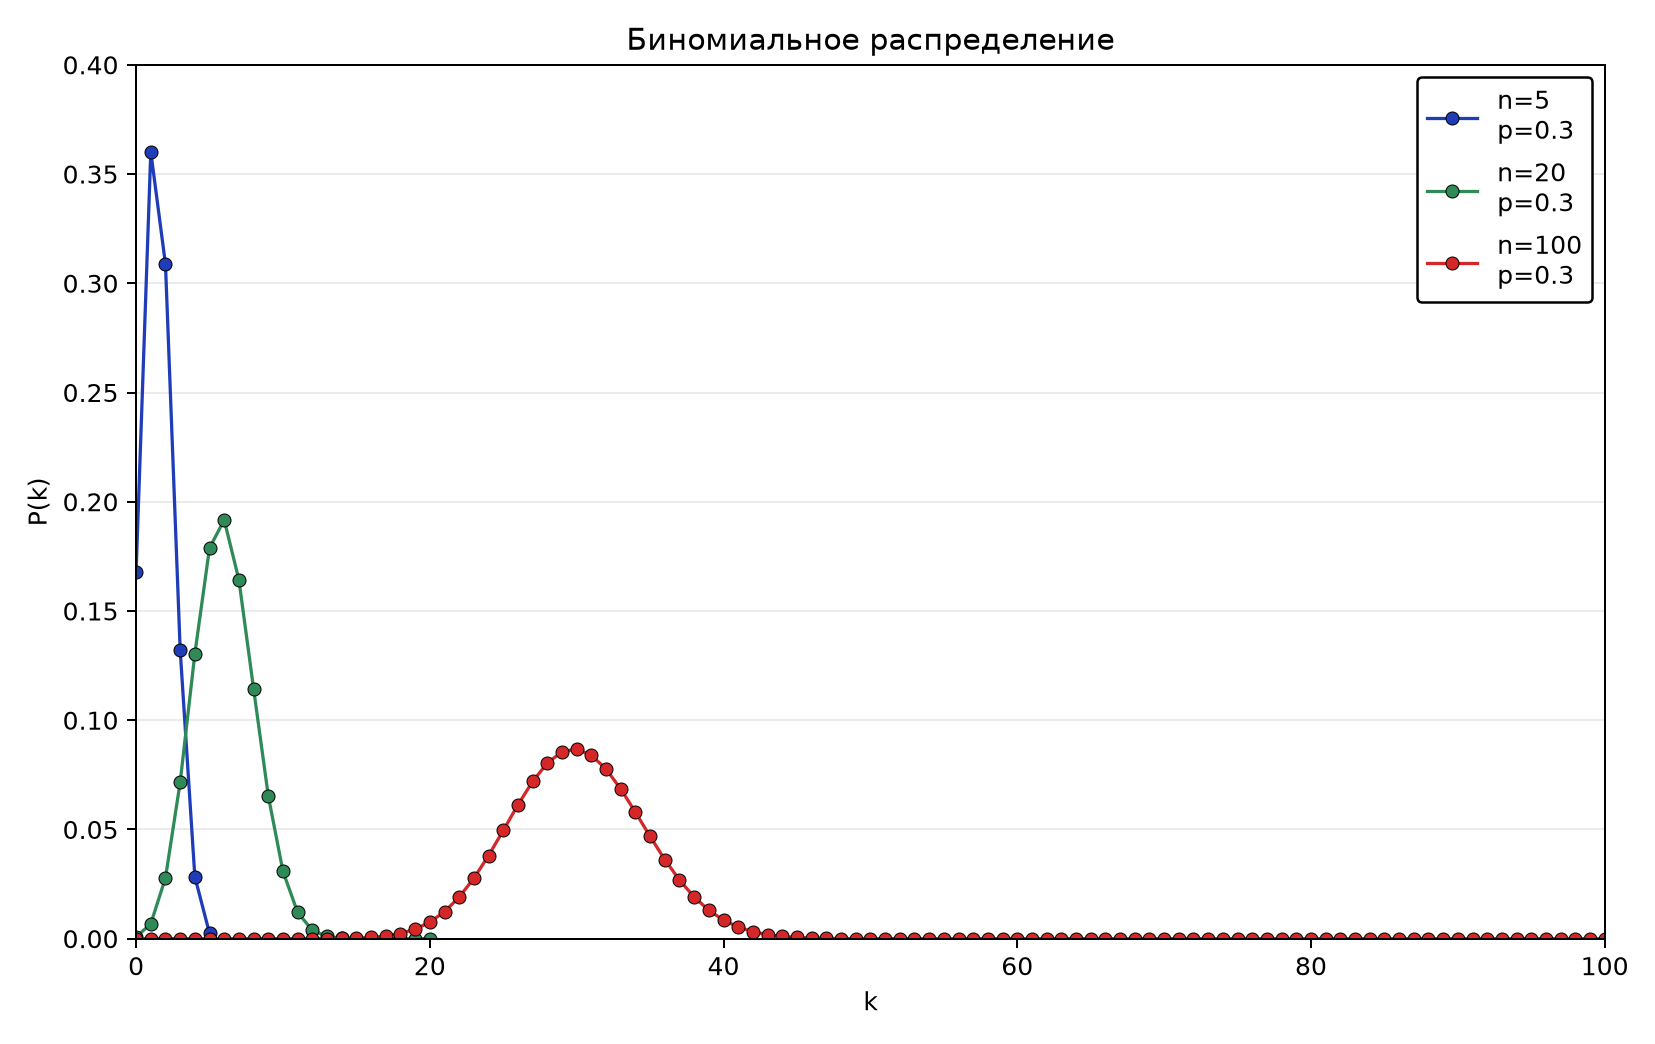
\includegraphics[keepaspectratio]{chapters/../assets/figures/binomial_pmf_profiles.png}}

}

\caption{\label{fig-binomial-pmf-profiles}Биномиальные распределения при
\(p=0.3\) и трёх значениях числа испытаний: \(n=5\), \(20\) и \(100\)}

\end{figure}%

С ростом \(n\) максимум смещается вслед за средним значением \(np\).
Абсолютная ширина распределения растёт как \(\sqrt{np(1-p)}\), а
относительная ширина уменьшается как \(1/\sqrt n\). При больших \(np\) и
\(n(1-p)\) форма становится близкой к гауссовой, хотя величина \(K\)
по-прежнему принимает только целые значения.

\subsection{Моменты биномиального
распределения}\label{ux43cux43eux43cux435ux43dux442ux44b-ux431ux438ux43dux43eux43cux438ux430ux43bux44cux43dux43eux433ux43e-ux440ux430ux441ux43fux440ux435ux434ux435ux43bux435ux43dux438ux44f}

Для биномиального распределения

\begin{equation}\protect\phantomsection\label{eq-binomial-moments}{
\mathbb E[K]=np,
\qquad
\operatorname{Var}(K)=np(1-p).
}\end{equation}

Выведем обе формулы. Этот вывод заодно показывает полезный приём с
факториальными моментами.

\begin{bookderivation}

\subsubsection{Среднее}\label{ux441ux440ux435ux434ux43dux435ux435}

Начнём с определения математического ожидания:

\[
\mathbb E[K]
=\sum_{k=0}^{n}k\binom{n}{k}p^k(1-p)^{n-k}.
\]

Используем тождество

\[
k\binom{n}{k}=n\binom{n-1}{k-1}.
\]

Тогда

\begin{equation}\protect\phantomsection\label{eq-binomial-mean}{
\begin{aligned}
\mathbb E[K]
&=np\sum_{k=1}^{n}
\binom{n-1}{k-1}p^{k-1}(1-p)^{n-k}\\
&=np\sum_{j=0}^{n-1}
\binom{n-1}{j}p^j(1-p)^{n-1-j}\\
&=np.
\end{aligned}
}\end{equation}

Последняя сумма равна единице по биному Ньютона.

\end{bookderivation}

\begin{bookderivation}

\subsubsection{Дисперсия}\label{ux434ux438ux441ux43fux435ux440ux441ux438ux44f-1}

Для вычисления дисперсии удобно начать с факториального момента
\(K(K-1)\):

\[
\mathbb E[K(K-1)]
=\sum_{k=0}^{n}k(k-1)\binom{n}{k}p^k(1-p)^{n-k}.
\]

Поскольку

\[
k(k-1)\binom{n}{k}
=n(n-1)\binom{n-2}{k-2},
\]

тот же приём даёт

\begin{equation}\protect\phantomsection\label{eq-binomial-second-factorial-moment}{
\mathbb E[K(K-1)]=n(n-1)p^2.
}\end{equation}

Обычный второй момент связан с факториальным тождеством

\[
K^2=K(K-1)+K.
\]

Поэтому

\begin{equation}\protect\phantomsection\label{eq-binomial-variance}{
\begin{aligned}
\operatorname{Var}(K)
&=\mathbb E[K^2]-\mathbb E[K]^2\\
&=n(n-1)p^2+np-n^2p^2\\
&=np(1-p).
\end{aligned}
}\end{equation}

\end{bookderivation}

\section{Счёт редких событий: пуассоновская
модель}\label{ux441ux447ux451ux442-ux440ux435ux434ux43aux438ux445-ux441ux43eux431ux44bux442ux438ux439-ux43fux443ux430ux441ux441ux43eux43dux43eux432ux441ux43aux430ux44f-ux43cux43eux434ux435ux43bux44c}

Теперь рассмотрим другой эксперимент. Радиоактивный источник работает в
течение заданного времени \(\Delta t\), а детектор считает распады.
Число испытаний заранее не фиксировано. Задана средняя частота
регистрации \(r\), и среднее число событий за время наблюдения равно

\begin{equation}\protect\phantomsection\label{eq-poisson-mean-rate}{
\lambda=r\,\Delta t.
}\end{equation}

Если интенсивность не меняется со временем, а события происходят
независимо, число зарегистрированных событий \(N\) подчиняется
распределению Пуассона.

\begin{booknote}

\textbf{Распределение Пуассона} задаётся функцией вероятностей

\begin{equation}\protect\phantomsection\label{eq-poisson-pmf}{
P(N=k)=\frac{\lambda^k e^{-\lambda}}{k!},
\qquad k=0,1,2,\ldots,
}\end{equation}

где \(\lambda>0\) --- среднее число событий. Короткая запись имеет вид

\[
N\sim\operatorname{Pois}(\lambda).
\]

\end{booknote}

\begin{semanticpdfbox}[colback=BookBiographySoft,borderline west={1.2mm}{0pt}{BookBiography},breakable=false]

\noindent\begin{minipage}[t]{30mm}\vspace{0pt}\centering

\href{https://mathshistory.st-andrews.ac.uk/Biographies/Poisson/pictdisplay/}{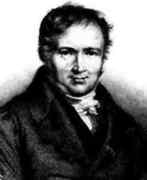
\includegraphics[width=28mm,height=\textheight,keepaspectratio,alt={Портрет Симеона Дени Пуассона}]{assets/people/simeon-poisson.jpg}}

\end{minipage}\hfill\begin{minipage}[t]{\dimexpr\linewidth-35mm\relax}\vspace{0pt}

{\sffamily\bfseries\footnotesize\color{BookBiography} БИОГРАФИЯ\par}\vspace{0.8mm}{\sffamily\bfseries\large\color{BookInk} Симеон Дени Пуассон\par}

{\sffamily\small\color{BookMuted} 1781–1840\par}\vspace{1.4mm}

Симеон Дени Пуассон --- французский математик и физик. Он работал над
теорией вероятностей, механикой, теорией упругости, электричеством и
магнетизмом. Распределение, носящее его имя, появилось в исследовании
вероятностей судебных решений и сегодня постоянно используется при
подсчёте событий в физическом эксперименте.

{\footnotesize\color{BookMuted}

\textbf{Источник:}
\href{https://mathshistory.st-andrews.ac.uk/Biographies/Poisson/}{MacTutor};
фото
\href{https://mathshistory.st-andrews.ac.uk/Biographies/Poisson/pictdisplay/}{MacTutor}

}

\end{minipage}

\end{semanticpdfbox}

\subsection{Пример распределения
Пуассона}\label{ux43fux440ux438ux43cux435ux440-ux440ux430ux441ux43fux440ux435ux434ux435ux43bux435ux43dux438ux44f-ux43fux443ux430ux441ux441ux43eux43dux430}

На рисунке \ref{fig-poisson-pmf-profiles} показаны распределения
Пуассона при \(\lambda=1\), \(4\) и \(10\).

\begin{Shaded}
\begin{Highlighting}[]
\ImportTok{from}\NormalTok{ math }\ImportTok{import}\NormalTok{ factorial}
\ImportTok{import}\NormalTok{ numpy }\ImportTok{as}\NormalTok{ np}

\ControlFlowTok{for}\NormalTok{ lam }\KeywordTok{in}\NormalTok{ [}\DecValTok{1}\NormalTok{, }\DecValTok{4}\NormalTok{, }\DecValTok{10}\NormalTok{]:}
\NormalTok{    k }\OperatorTok{=}\NormalTok{ np.arange(}\DecValTok{26}\NormalTok{)}
\NormalTok{    pmf }\OperatorTok{=}\NormalTok{ np.exp(}\OperatorTok{{-}}\NormalTok{lam) }\OperatorTok{*}\NormalTok{ lam}\OperatorTok{**}\NormalTok{k }\OperatorTok{/}\NormalTok{ np.array([factorial(i) }\ControlFlowTok{for}\NormalTok{ i }\KeywordTok{in}\NormalTok{ k])}
\end{Highlighting}
\end{Shaded}

\begin{figure}

\centering{

\pandocbounded{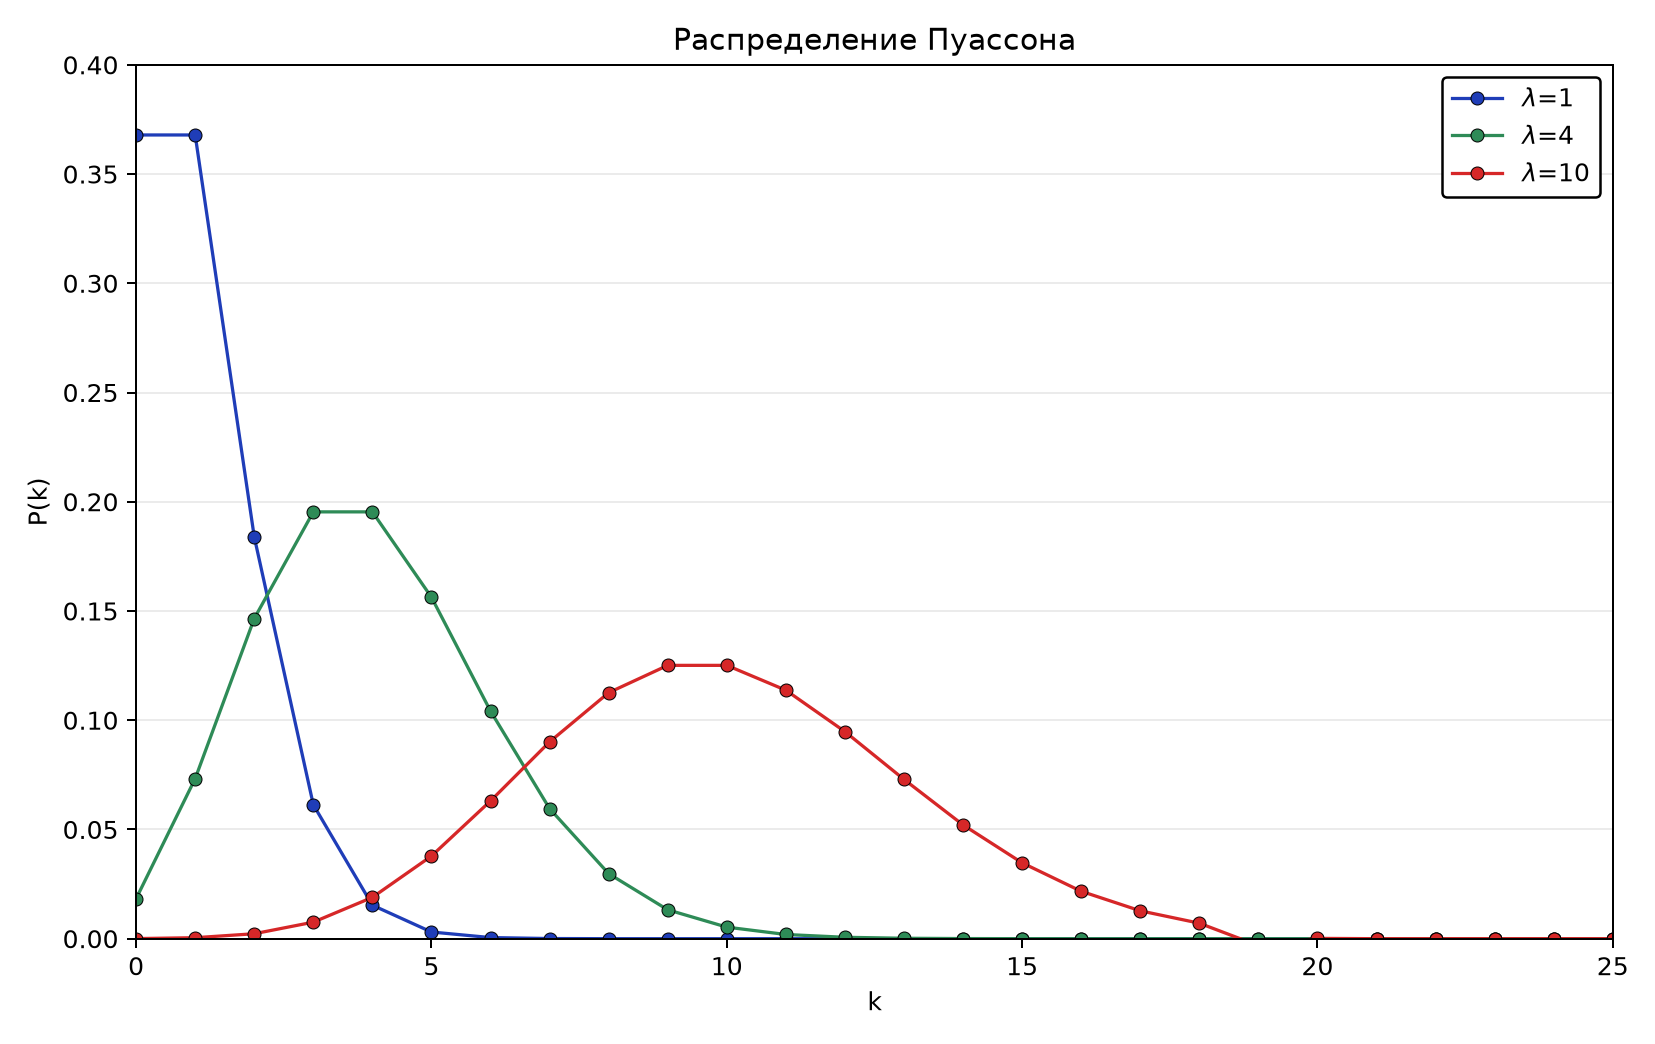
\includegraphics[keepaspectratio]{chapters/../assets/figures/poisson_pmf_profiles.png}}

}

\caption{\label{fig-poisson-pmf-profiles}Распределения Пуассона при
среднем числе событий \(\lambda=1\), \(4\) и \(10\)}

\end{figure}%

При \(\lambda=1\) основная вероятность сосредоточена около нуля и
распределение заметно асимметрично. С ростом \(\lambda\) максимум
смещается вправо, ширина увеличивается, а форма становится всё более
симметричной. При больших \(\lambda\) распределение Пуассона можно
приближать нормальным распределением. Условия и точность такого
приближения мы обсудим в главе о центральной предельной теореме.

\subsection{Моменты распределения
Пуассона}\label{ux43cux43eux43cux435ux43dux442ux44b-ux440ux430ux441ux43fux440ux435ux434ux435ux43bux435ux43dux438ux44f-ux43fux443ux430ux441ux441ux43eux43dux430}

У распределения Пуассона среднее и дисперсия равны одному и тому же
параметру:

\begin{equation}\protect\phantomsection\label{eq-poisson-moments}{
\mathbb E[N]=\lambda,
\qquad
\operatorname{Var}(N)=\lambda.
}\end{equation}

\begin{bookderivation}

\subsubsection{Среднее}\label{ux441ux440ux435ux434ux43dux435ux435-1}

По определению математического ожидания

\[
\mathbb E[N]
=\sum_{k=0}^{\infty}k\frac{\lambda^k e^{-\lambda}}{k!}.
\]

Слагаемое при \(k=0\) равно нулю. В остальных слагаемых вынесем один
множитель \(\lambda\) и сдвинем индекс \(j=k-1\):

\begin{equation}\protect\phantomsection\label{eq-poisson-mean}{
\begin{aligned}
\mathbb E[N]
&=\lambda e^{-\lambda}
\sum_{k=1}^{\infty}\frac{\lambda^{k-1}}{(k-1)!}\\
&=\lambda e^{-\lambda}
\sum_{j=0}^{\infty}\frac{\lambda^j}{j!}\\
&=\lambda e^{-\lambda}e^\lambda
=\lambda.
\end{aligned}
}\end{equation}

\end{bookderivation}

\begin{bookderivation}

\subsubsection{Дисперсия}\label{ux434ux438ux441ux43fux435ux440ux441ux438ux44f-2}

Снова начнём со второго факториального момента:

\[
\mathbb E[N(N-1)]
=\sum_{k=0}^{\infty}
k(k-1)\frac{\lambda^k e^{-\lambda}}{k!}.
\]

Первые два слагаемых равны нулю, а при \(k\geq2\)

\[
\frac{k(k-1)}{k!}=\frac{1}{(k-2)!}.
\]

Отсюда

\begin{equation}\protect\phantomsection\label{eq-poisson-second-factorial-moment}{
\begin{aligned}
\mathbb E[N(N-1)]
&=\lambda^2e^{-\lambda}
\sum_{k=2}^{\infty}\frac{\lambda^{k-2}}{(k-2)!}\\
&=\lambda^2e^{-\lambda}
\sum_{j=0}^{\infty}\frac{\lambda^j}{j!}\\
&=\lambda^2.
\end{aligned}
}\end{equation}

Используя \(N^2=N(N-1)+N\), получаем

\begin{equation}\protect\phantomsection\label{eq-poisson-variance}{
\begin{aligned}
\operatorname{Var}(N)
&=\mathbb E[N^2]-\mathbb E[N]^2\\
&=\lambda^2+\lambda-\lambda^2\\
&=\lambda.
\end{aligned}
}\end{equation}

\end{bookderivation}

\section{Непрерывные ошибки: нормальная
модель}\label{ux43dux435ux43fux440ux435ux440ux44bux432ux43dux44bux435-ux43eux448ux438ux431ux43aux438-ux43dux43eux440ux43cux430ux43bux44cux43dux430ux44f-ux43cux43eux434ux435ux43bux44c}

Биномиальное и пуассоновское распределения описывают целое число
событий. Результат измерения энергии, времени или координаты обычно
рассматривается как непрерывная величина. Самая известная модель для
такой величины --- нормальное, или гауссово, распределение.

\begin{booknote}

\textbf{Нормальное распределение} с параметрами \(\mu\) и \(\sigma>0\)
имеет плотность

\begin{equation}\protect\phantomsection\label{eq-normal-density}{
f(x;\mu,\sigma)
=\frac{1}{\sigma\sqrt{2\pi}}
\exp\!\left[-\frac{(x-\mu)^2}{2\sigma^2}\right].
}\end{equation}

Здесь \(\mu\) --- среднее значение, а \(\sigma\) --- стандартное
отклонение. Короткая запись имеет вид

\[
X\sim\mathcal N(\mu,\sigma^2).
\]

\end{booknote}

Почему это распределение называется нормальным? Карл Пирсон, который
ввёл это название в широкое употребление, позднее заметил его неудачную
сторону:

\begin{quote}
Много лет назад я назвал кривую Лапласа-Гаусса нормальной кривой. Это
название, избегая международного спора о приоритете, имеет недостаток:
оно заставляет думать, что все прочие распределения частот в том или
ином смысле «ненормальны».

К. Пирсон, 1920 {[}2{]}
\end{quote}

Причина частого появления гауссовой формы связана с центральной
предельной теоремой. Сумма большого числа малых независимых вкладов при
достаточно общих условиях приближается нормальным распределением. Этому
будет посвящена отдельная глава.

\subsection{Пример нормального
распределения}\label{ux43fux440ux438ux43cux435ux440-ux43dux43eux440ux43cux430ux43bux44cux43dux43eux433ux43e-ux440ux430ux441ux43fux440ux435ux434ux435ux43bux435ux43dux438ux44f}

На рисунке \ref{fig-normal-density-profiles} показаны три плотности с
параметрами \((\mu,\sigma)=(0,1)\), \((0,2)\) и \((2,1)\).

\begin{Shaded}
\begin{Highlighting}[]
\ImportTok{import}\NormalTok{ numpy }\ImportTok{as}\NormalTok{ np}

\NormalTok{x }\OperatorTok{=}\NormalTok{ np.linspace(}\OperatorTok{{-}}\DecValTok{6}\NormalTok{, }\DecValTok{6}\NormalTok{, }\DecValTok{400}\NormalTok{)}
\ControlFlowTok{for}\NormalTok{ mu, sigma }\KeywordTok{in}\NormalTok{ [(}\DecValTok{0}\NormalTok{, }\DecValTok{1}\NormalTok{), (}\DecValTok{0}\NormalTok{, }\DecValTok{2}\NormalTok{), (}\DecValTok{2}\NormalTok{, }\DecValTok{1}\NormalTok{)]:}
\NormalTok{    pdf }\OperatorTok{=}\NormalTok{ np.exp(}\OperatorTok{{-}}\FloatTok{0.5}\OperatorTok{*}\NormalTok{((x}\OperatorTok{{-}}\NormalTok{mu)}\OperatorTok{/}\NormalTok{sigma)}\OperatorTok{**}\DecValTok{2}\NormalTok{)}\OperatorTok{/}\NormalTok{(sigma}\OperatorTok{*}\NormalTok{np.sqrt(}\DecValTok{2}\OperatorTok{*}\NormalTok{np.pi))}
\end{Highlighting}
\end{Shaded}

\begin{figure}

\centering{

\pandocbounded{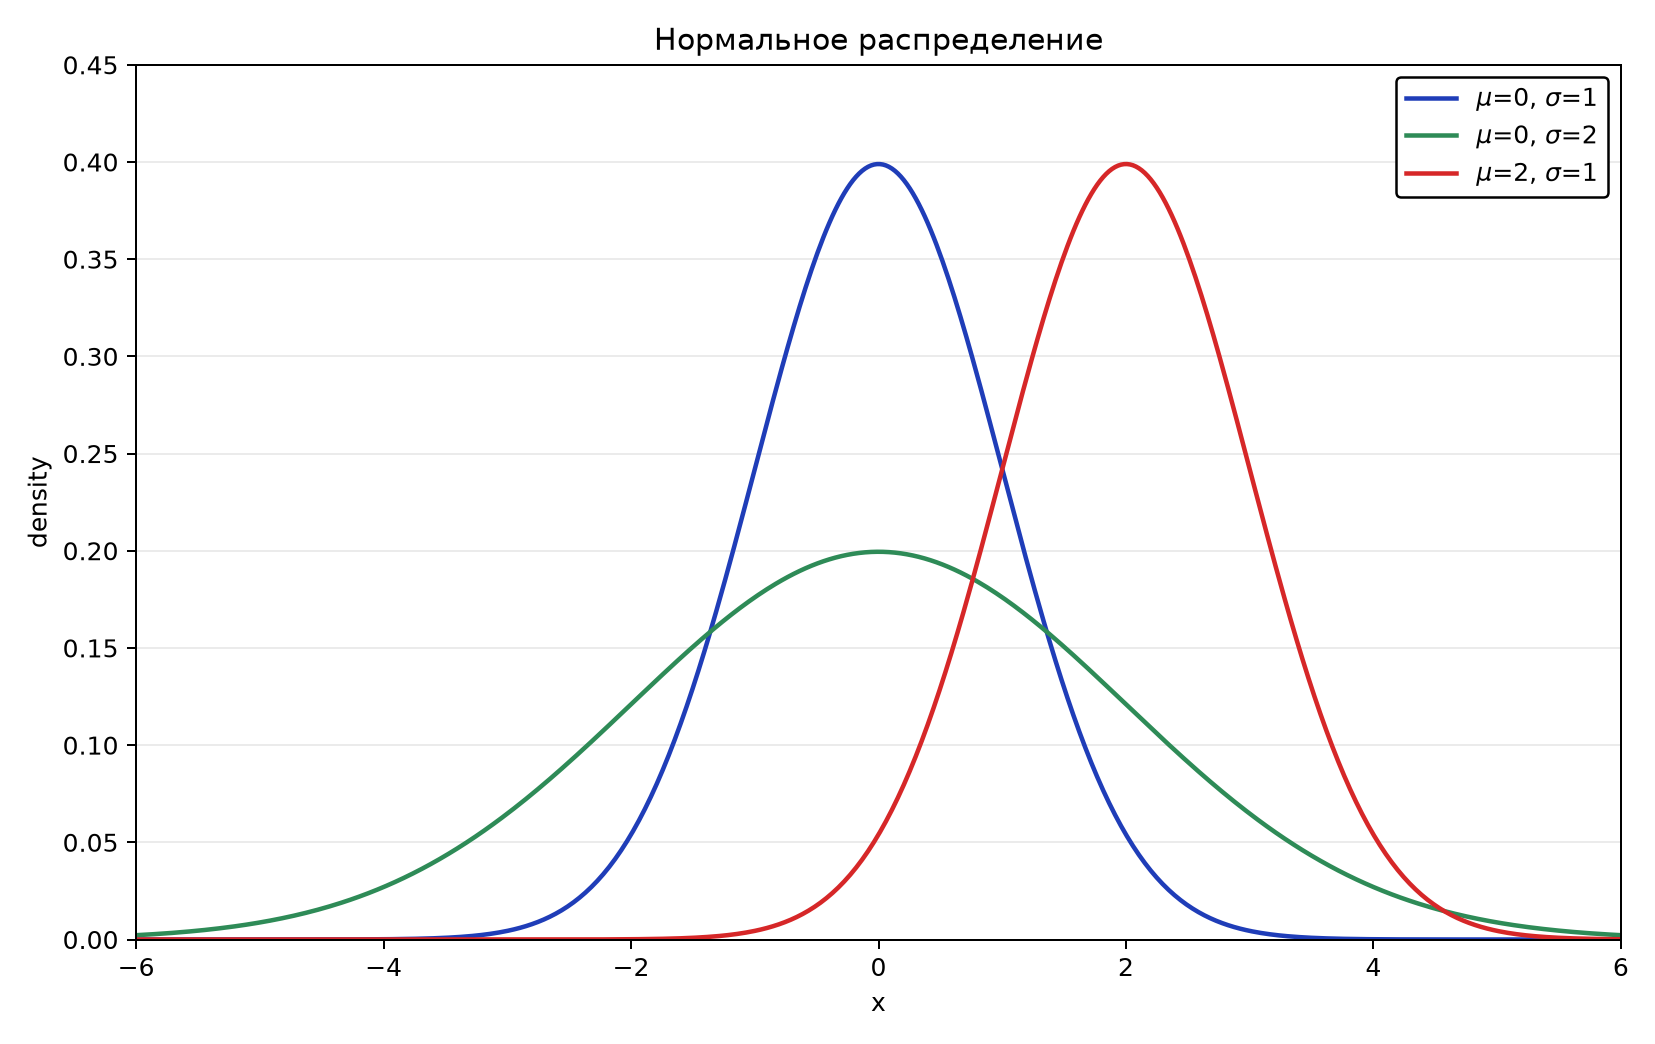
\includegraphics[keepaspectratio]{chapters/../assets/figures/normal_density_profiles.png}}

}

\caption{\label{fig-normal-density-profiles}Плотности нормального
распределения при \((\mu,\sigma)=(0,1)\), \((0,2)\) и \((2,1)\)}

\end{figure}%

Синие и красные кривые имеют одинаковую ширину \(\sigma=1\) и разные
средние: изменение \(\mu\) сдвигает распределение вдоль оси \(x\). У
зелёной кривой \(\sigma=2\), поэтому она шире и ниже. Площадь под каждой
кривой по-прежнему равна единице.

\subsection{Моменты распределения
Гаусса}\label{ux43cux43eux43cux435ux43dux442ux44b-ux440ux430ux441ux43fux440ux435ux434ux435ux43bux435ux43dux438ux44f-ux433ux430ux443ux441ux441ux430}

Параметры нормального распределения совпадают с его средним и
стандартным отклонением:

\begin{equation}\protect\phantomsection\label{eq-normal-moments}{
\mathbb E[X]=\mu,
\qquad
\operatorname{Var}(X)=\sigma^2.
}\end{equation}

\begin{bookderivation}

\subsubsection{Среднее}\label{ux441ux440ux435ux434ux43dux435ux435-2}

Перейдём к стандартной нормальной величине

\[
z=\frac{x-\mu}{\sigma},
\qquad
x=\mu+\sigma z,
\qquad
dx=\sigma\,dz,
\]

плотность которой обозначим

\begin{equation}\protect\phantomsection\label{eq-standard-normal-density}{
\varphi(z)=\frac{1}{\sqrt{2\pi}}e^{-z^2/2}.
}\end{equation}

Тогда

\begin{equation}\protect\phantomsection\label{eq-normal-mean}{
\begin{aligned}
\mathbb E[X]
&=\int_{-\infty}^{+\infty}(\mu+\sigma z)\varphi(z)\,dz\\
&=\mu\int_{-\infty}^{+\infty}\varphi(z)\,dz
+\sigma\int_{-\infty}^{+\infty}z\varphi(z)\,dz\\
&=\mu.
\end{aligned}
}\end{equation}

Первый интеграл равен единице по условию нормировки. Второй равен нулю,
потому что \(z\varphi(z)\) --- нечётная функция.

\end{bookderivation}

\begin{bookderivation}

\subsubsection{Дисперсия}\label{ux434ux438ux441ux43fux435ux440ux441ux438ux44f-3}

Та же замена переменной даёт

\[
\operatorname{Var}(X)
=\sigma^2\int_{-\infty}^{+\infty}z^2\varphi(z)\,dz.
\]

Оставшийся интеграл вычислим по частям. Поскольку

\[
\varphi'(z)=-z\varphi(z),
\]

получаем

\[
\begin{aligned}
\int_{-\infty}^{+\infty}z^2\varphi(z)\,dz
&=\left[-z\varphi(z)\right]_{-\infty}^{+\infty}
+\int_{-\infty}^{+\infty}\varphi(z)\,dz\\
&=1.
\end{aligned}
\]

Следовательно,

\begin{equation}\protect\phantomsection\label{eq-normal-variance}{
\operatorname{Var}(X)=\sigma^2.
}\end{equation}

\end{bookderivation}

\section{Сравнение трёх
распределений}\label{ux441ux440ux430ux432ux43dux435ux43dux438ux435-ux442ux440ux451ux445-ux440ux430ux441ux43fux440ux435ux434ux435ux43bux435ux43dux438ux439}

В таблице \ref{tbl-basic-distributions} собраны три рассмотренные
модели. В последнем столбце перечислены условия, которые относятся к
устройству повторяемого эксперимента.

\begin{longtable}[]{@{}
  >{\raggedright\arraybackslash}p{(\linewidth - 6\tabcolsep) * \real{0.2222}}
  >{\centering\arraybackslash}p{(\linewidth - 6\tabcolsep) * \real{0.2778}}
  >{\centering\arraybackslash}p{(\linewidth - 6\tabcolsep) * \real{0.2778}}
  >{\raggedright\arraybackslash}p{(\linewidth - 6\tabcolsep) * \real{0.2222}}@{}}
\caption{Основные свойства биномиального, пуассоновского и нормального
распределений}\label{tbl-basic-distributions}\tabularnewline
\toprule\noalign{}
\begin{minipage}[b]{\linewidth}\raggedright
Распределение
\end{minipage} & \begin{minipage}[b]{\linewidth}\centering
Среднее
\end{minipage} & \begin{minipage}[b]{\linewidth}\centering
Дисперсия
\end{minipage} & \begin{minipage}[b]{\linewidth}\raggedright
Условия применения
\end{minipage} \\
\midrule\noalign{}
\endfirsthead
\toprule\noalign{}
\begin{minipage}[b]{\linewidth}\raggedright
Распределение
\end{minipage} & \begin{minipage}[b]{\linewidth}\centering
Среднее
\end{minipage} & \begin{minipage}[b]{\linewidth}\centering
Дисперсия
\end{minipage} & \begin{minipage}[b]{\linewidth}\raggedright
Условия применения
\end{minipage} \\
\midrule\noalign{}
\endhead
\bottomrule\noalign{}
\endlastfoot
\(K\sim\operatorname{Bin}(n,p)\) & \(np\) & \(np(1-p)\) & Фиксированное
\(n\); независимые испытания; постоянное \(p\) \\
\(N\sim\operatorname{Pois}(\lambda)\) & \(\lambda\) & \(\lambda\) & Счёт
событий в фиксированном интервале; постоянная интенсивность;
независимость \\
\(X\sim\mathcal N(\mu,\sigma^2)\) & \(\mu\) & \(\sigma^2\) & Непрерывная
величина; приближение для суммы многих малых независимых вкладов \\
\end{longtable}

\begin{bookchaptersummary}[Итоги главы]

\begin{itemize}
\tightlist
\item
  Случайная величина описывается распределением. Для дискретной величины
  оно задаёт вероятности отдельных значений, для непрерывной ---
  плотность вероятности.
\item
  Математическое ожидание указывает центр распределения, а дисперсия
  измеряет средний квадрат отклонения от этого центра. Эти величины
  существуют только при сходимости соответствующих суммы или интеграла.
\item
  Биномиальное распределение относится к фиксированному числу испытаний,
  распределение Пуассона --- к числу событий в фиксированном интервале,
  а нормальное распределение --- к непрерывной величине.
\item
  Выбор распределения включает условия, при которых повторяется
  эксперимент: независимость испытаний, постоянство вероятности или
  интенсивности и способ набора данных.
\end{itemize}

\end{bookchaptersummary}

\section{Задачи}\label{ux437ux430ux434ux430ux447ux438-1}

\begin{semanticpdfbox}[colback=BookCoralSoft,borderline west={1.2mm}{0pt}{BookCoral},breakable=false]

\noindent{\sffamily\bfseries\fontsize{11.2}{13.5}\selectfont Задача 1. Предел биномиального распределения}\par\nopagebreak[4]\vspace{1.2mm}

Покажите, что при \[
n\to\infty,\qquad p\to 0,\qquad np=\lambda=\text{const}
\] биномиальное распределение переходит в распределение Пуассона: \[
\binom{n}{k}p^k(1-p)^{n-k}
\longrightarrow
\frac{\lambda^k e^{-\lambda}}{k!}.
\]

\textbf{Подсказка.} Положите \(p=\lambda/n\) и рассмотрите предел при
фиксированном \(k\).

\end{semanticpdfbox}

\begin{semanticpdfbox}[colback=BookCoralSoft,borderline west={1.2mm}{0pt}{BookCoral},breakable=false]

\noindent{\sffamily\bfseries\fontsize{11.2}{13.5}\selectfont Задача 2. Предел Пуассона к гауссову распределению}\par\nopagebreak[4]\vspace{1.2mm}

Используя формулу Стирлинга, покажите, что при больших \(\lambda\) \[
P(N=n)\approx
\frac{1}{\sqrt{2\pi\lambda}}
\exp\!\left[-\frac{(n-\lambda)^2}{2\lambda}\right].
\]

\end{semanticpdfbox}

\begin{semanticpdfbox}[colback=BookCoralSoft,borderline west={1.2mm}{0pt}{BookCoral},breakable=false]

\noindent{\sffamily\bfseries\fontsize{11.2}{13.5}\selectfont Задача 3. Моменты равномерного распределения}\par\nopagebreak[4]\vspace{1.2mm}

Пусть \(X\sim U(-1,1)\). Найдите:

\begin{enumerate}
\def\labelenumi{\arabic{enumi}.}
\tightlist
\item
  \(\mathbb{E}[X]\);
\item
  \(\mathbb{E}[X^2]\);
\item
  \(\mathrm{Var}(X)\).
\end{enumerate}

\end{semanticpdfbox}

\begin{semanticpdfbox}[colback=BookCoralSoft,borderline west={1.2mm}{0pt}{BookCoral},breakable=false]

\noindent{\sffamily\bfseries\fontsize{11.2}{13.5}\selectfont Задача 4. Когда моменты однозначно задают распределение}\par\nopagebreak[4]\vspace{1.2mm}

Пусть \[
\mathbb{E}[X^{2n}]=1,\qquad
\mathbb{E}[X^{2n+1}]=0.
\] Покажите, что \(X=\pm1\) с равными вероятностями.

\textbf{Подсказка.} Используйте \(\mathbb{E}[(X^2-1)^2]=0\).

\end{semanticpdfbox}

\begin{semanticpdfbox}[colback=BookCoralSoft,borderline west={1.2mm}{0pt}{BookCoral},breakable=false]

\noindent{\sffamily\bfseries\fontsize{11.2}{13.5}\selectfont Задача 5. Восстановление распределения на конечном носителе}\par\nopagebreak[4]\vspace{1.2mm}

Пусть \(X\) принимает значения \(-1\), \(0\), \(1\), причём \[
\mathbb{E}[X]=0,\qquad
\mathbb{E}[X^2]=\frac{1}{2}.
\] Найдите вероятности трёх значений.

\end{semanticpdfbox}

\begin{semanticpdfbox}[colback=BookCoralSoft,borderline west={1.2mm}{0pt}{BookCoral},breakable=false]

\noindent{\sffamily\bfseries\fontsize{11.2}{13.5}\selectfont Задача 6. Факториальные моменты распределения Пуассона}\par\nopagebreak[4]\vspace{1.2mm}

Для \(N\sim\mathrm{Pois}(\lambda)\) покажите, что \[
\mathbb{E}[N(N-1)\cdots(N-r+1)]=\lambda^r.
\]

\end{semanticpdfbox}

\section*{Литература}\label{ux43bux438ux442ux435ux440ux430ux442ux443ux440ux430-1}
\addcontentsline{toc}{section}{Литература}

\markright{Литература}

\protect\phantomsection\label{refs}
\begin{CSLReferences}{0}{0}
\bibitem[\citeproctext]{ref-feller1971}
{[}1{]} Feller, W. \emph{An Introduction to Probability Theory and Its
Applications}. John Wiley \& Sons. 1971.

\bibitem[\citeproctext]{ref-pearson1920correlation}
{[}2{]} Pearson, K. Notes on the History of Correlation.
\emph{Biometrika}, \textbf{13}, 25--45. 1920.
doi:\href{https://doi.org/10.1093/biomet/13.1.25}{10.1093/biomet/13.1.25}.

\end{CSLReferences}

\chapter{Характеристические функции и суммы случайных
величин}\label{ux445ux430ux440ux430ux43aux442ux435ux440ux438ux441ux442ux438ux447ux435ux441ux43aux438ux435-ux444ux443ux43dux43aux446ux438ux438-ux438-ux441ux443ux43cux43cux44b-ux441ux43bux443ux447ux430ux439ux43dux44bux445-ux432ux435ux43bux438ux447ux438ux43d}

\bookchapteropeningcontents

\begin{bookchapteropening}[Аннотация]

В этой главе мы научимся находить распределение суммы независимых
случайных величин. Прямой путь приводит к свёртке плотностей.
Преобразование Фурье заменяет свёртку произведением и вводит
характеристическую функцию. На нескольких знакомых распределениях мы
разберём, как она работает, извлечём из неё моменты и кумулянты и
подойдём к центральной предельной теореме.

\end{bookchapteropening}

\section{Распределение суммы независимых случайных
величин}\label{ux440ux430ux441ux43fux440ux435ux434ux435ux43bux435ux43dux438ux435-ux441ux443ux43cux43cux44b-ux43dux435ux437ux430ux432ux438ux441ux438ux43cux44bux445-ux441ux43bux443ux447ux430ux439ux43dux44bux445-ux432ux435ux43bux438ux447ux438ux43d}

Пусть \(X\) и \(Y\) --- независимые случайные величины с плотностями
\(f_X(x)\) и \(f_Y(y)\). Нас интересует сумма

\begin{equation}\protect\phantomsection\label{eq-sum-two-random-variables}{
S=X+Y.
}\end{equation}

Такая задача постоянно возникает в эксперименте. Полное энерговыделение
складывается из энерговыделений отдельных частиц, заряд на выходе
детектора --- из зарядов отдельных фотоэлектронов, а результат измерения
--- из сигнала и шума.

Значение \(S=s\) можно получить из любой пары \((x,y)\), для которой
\(x+y=s\). После выбора \(x\) второе слагаемое равно \(s-x\).
Независимость позволяет перемножить плотности, а интегрирование собирает
вклады от всех возможных \(x\):

\begin{equation}\protect\phantomsection\label{eq-convolution-density}{
f_S(s)=
\int_{-\infty}^{+\infty}
f_X(x)f_Y(s-x)\,dx.
}\end{equation}

Интеграл в формуле \ref{eq-convolution-density} называется
\textbf{свёрткой}. Для него используется короткая запись

\begin{equation}\protect\phantomsection\label{eq-convolution-notation}{
f_S=f_X*f_Y.
}\end{equation}

Звёздочка здесь обозначает операцию свёртки. Условие независимости
существенно: для зависимых величин произведение \(f_X(x)f_Y(s-x)\) нужно
заменить совместной плотностью \(f_{X,Y}(x,s-x)\).

\subsection{Сумма нескольких
величин}\label{ux441ux443ux43cux43cux430-ux43dux435ux441ux43aux43eux43bux44cux43aux438ux445-ux432ux435ux43bux438ux447ux438ux43d}

Для суммы

\begin{equation}\protect\phantomsection\label{eq-sum-many-random-variables}{
S_n=X_1+X_2+\dots+X_n
}\end{equation}

получается последовательная свёртка:

\begin{equation}\protect\phantomsection\label{eq-convolution-many}{
f_{S_n}=f_{X_1}*f_{X_2}*\cdots*f_{X_n}.
}\end{equation}

В развёрнутом виде это \((n-1)\)-кратный интеграл:

\begin{equation}\protect\phantomsection\label{eq-convolution-many-integral}{
\begin{aligned}
f_{S_n}(s)
={}&\int_{-\infty}^{+\infty}\!\cdots
\int_{-\infty}^{+\infty}
f_{X_1}(x_1)\cdots f_{X_{n-1}}(x_{n-1})\\
&\times
f_{X_n}(s-x_1-\cdots-x_{n-1})
\,dx_1\cdots dx_{n-1}.
\end{aligned}
}\end{equation}

Каждое новое слагаемое добавляет ещё одно интегрирование. Формула верна
и полезна, но с ростом размерности интеграла вычислять его
непосредственно хочется всё меньше.

\section{Пример: распределение
Коши}\label{ux43fux440ux438ux43cux435ux440-ux440ux430ux441ux43fux440ux435ux434ux435ux43bux435ux43dux438ux435-ux43aux43eux448ux438}

Распределение Коши с параметром положения \(x_0\) и масштабом
\(\gamma>0\) имеет плотность

\begin{equation}\protect\phantomsection\label{eq-cauchy-density}{
f_X(x;x_0,\gamma)=
\frac{1}{
\pi\gamma\left[1+\left(\dfrac{x-x_0}{\gamma}\right)^2\right]}.
}\end{equation}

Та же форма известна как распределение Лоренца. В физике частиц она
связана с нерелятивистской формой линии Брейта---Вигнера, а в
спектроскопии описывает лоренцев профиль линии. Релятивистская форма
Брейта---Вигнера записывается иначе, поэтому считать эти названия
полными синонимами не следует.

При \(x_0=0\) и \(\gamma=1\) получаем стандартное распределение Коши:

\begin{equation}\protect\phantomsection\label{eq-standard-cauchy-density}{
f_X(x)=\frac{1}{\pi(1+x^2)}.
}\end{equation}

\begin{semanticpdfbox}[colback=BookBiographySoft,borderline west={1.2mm}{0pt}{BookBiography},breakable=false]

\noindent\begin{minipage}[t]{30mm}\vspace{0pt}\centering

\href{https://mathshistory.st-andrews.ac.uk/Biographies/Cauchy/pictdisplay/}{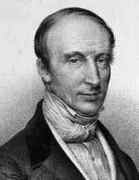
\includegraphics[width=28mm,height=\textheight,keepaspectratio,alt={Портрет Огюстена Луи Коши}]{assets/people/augustin-cauchy.jpg}}

\end{minipage}\hfill\begin{minipage}[t]{\dimexpr\linewidth-35mm\relax}\vspace{0pt}

{\sffamily\bfseries\footnotesize\color{BookBiography} БИОГРАФИЯ\par}\vspace{0.8mm}{\sffamily\bfseries\large\color{BookInk} Огюстен Луи Коши\par}

{\sffamily\small\color{BookMuted} 1789–1857\par}\vspace{1.4mm}

Французский математик и инженер. Коши внёс определяющий вклад в
математический анализ, дифференциальные уравнения и математическую
физику. Распределение Коши служит важным примером тяжёлых хвостов: его
математическое ожидание и дисперсия не существуют.

{\footnotesize\color{BookMuted}

\textbf{Источник:}
\href{https://mathshistory.st-andrews.ac.uk/Biographies/Cauchy/}{MacTutor};
фото
\href{https://mathshistory.st-andrews.ac.uk/Biographies/Cauchy/pictdisplay/}{MacTutor}

}

\end{minipage}

\end{semanticpdfbox}

Возьмём две независимые величины

\begin{equation}\protect\phantomsection\label{eq-two-standard-cauchy-variables}{
X,Y\sim\operatorname{Cauchy}(0,1).
}\end{equation}

Для суммы \(S=X+Y\) формула свёртки даёт

\begin{equation}\protect\phantomsection\label{eq-cauchy-direct-convolution}{
f_S(s)=
\frac{1}{\pi^2}
\int_{-\infty}^{+\infty}
\frac{dx}{(1+x^2)\left[1+(s-x)^2\right]}.
}\end{equation}

В знаменателе стоит многочлен четвёртой степени по \(x\). Интеграл можно
взять разложением на простые дроби или методом вычетов, после чего ответ
ещё придётся упростить. Задача поставлена одной строкой, а вычисление
уже разрослось. Для суммы многих величин этот путь становится совсем
непрактичным.

\section{Характеристическая
функция}\label{ux445ux430ux440ux430ux43aux442ux435ux440ux438ux441ux442ux438ux447ux435ux441ux43aux430ux44f-ux444ux443ux43dux43aux446ux438ux44f}

Вместо самой плотности рассмотрим её преобразование Фурье. Для случайной
величины \(X\) \textbf{характеристическая функция} определяется как
{[}1{]}

\begin{equation}\protect\phantomsection\label{eq-characteristic-definition}{
\varphi_X(t)=\mathbb E\!\left[e^{itX}\right].
}\end{equation}

Если \(X\) имеет плотность, математическое ожидание в формуле
\ref{eq-characteristic-definition} записывается интегралом:

\begin{equation}\protect\phantomsection\label{eq-characteristic-continuous}{
\varphi_X(t)=
\int_{-\infty}^{+\infty}e^{itx}f_X(x)\,dx.
}\end{equation}

Здесь \(x\) --- переменная интегрирования, а \(t\) --- аргумент
характеристической функции. Само распределение вещественно, но его
Фурье-образ в общем случае комплексный.

Характеристическая функция однозначно определяет распределение. Если
плотность существует и выполнены обычные условия теоремы обращения
Фурье, её можно восстановить по формуле

\begin{equation}\protect\phantomsection\label{eq-characteristic-inversion}{
f_X(x)=
\frac{1}{2\pi}
\int_{-\infty}^{+\infty}
e^{-itx}\varphi_X(t)\,dt.
}\end{equation}

Преобразование Фурье переводит свёртку в произведение. Для независимых
\(X\) и \(Y\) это видно непосредственно:

\begin{equation}\protect\phantomsection\label{eq-characteristic-independent-sum}{
\begin{aligned}
\varphi_{X+Y}(t)
&=\mathbb E\!\left[e^{it(X+Y)}\right]\\
&=\mathbb E\!\left[e^{itX}e^{itY}\right]\\
&=\mathbb E\!\left[e^{itX}\right]
  \mathbb E\!\left[e^{itY}\right]\\
&=\varphi_X(t)\varphi_Y(t).
\end{aligned}
}\end{equation}

Третье равенство и есть место, где используется независимость.

\section{Сумма двух величин Коши через характеристические
функции}\label{interactive-cauchy-sum}

Характеристическая функция стандартного распределения Коши равна

\begin{equation}\protect\phantomsection\label{eq-cauchy-characteristic}{
\varphi_X(t)=e^{-|t|}.
}\end{equation}

Её можно получить из формулы \ref{eq-standard-cauchy-density} методом
вычетов. Для двух независимых стандартных величин Коши формула
\ref{eq-characteristic-independent-sum} сразу даёт

\begin{equation}\protect\phantomsection\label{eq-cauchy-sum-characteristic}{
\varphi_{X+Y}(t)
=e^{-|t|}e^{-|t|}
=e^{-2|t|}.
}\end{equation}

Последнее выражение является характеристической функцией распределения
Коши с масштабом \(\gamma=2\). Поэтому

\begin{equation}\protect\phantomsection\label{eq-cauchy-sum-distribution}{
S=X+Y\sim\operatorname{Cauchy}(0,2),
\qquad
f_S(s)=\frac{2}{\pi(s^2+4)}.
}\end{equation}

Мы получили ответ, не вычисляя интеграл
\ref{eq-cauchy-direct-convolution}.

Стандартное распределение Коши и распределение суммы двух независимых
стандартных величин Коши.

\begin{semanticpdfbox}[breakable=false]

\begin{center}

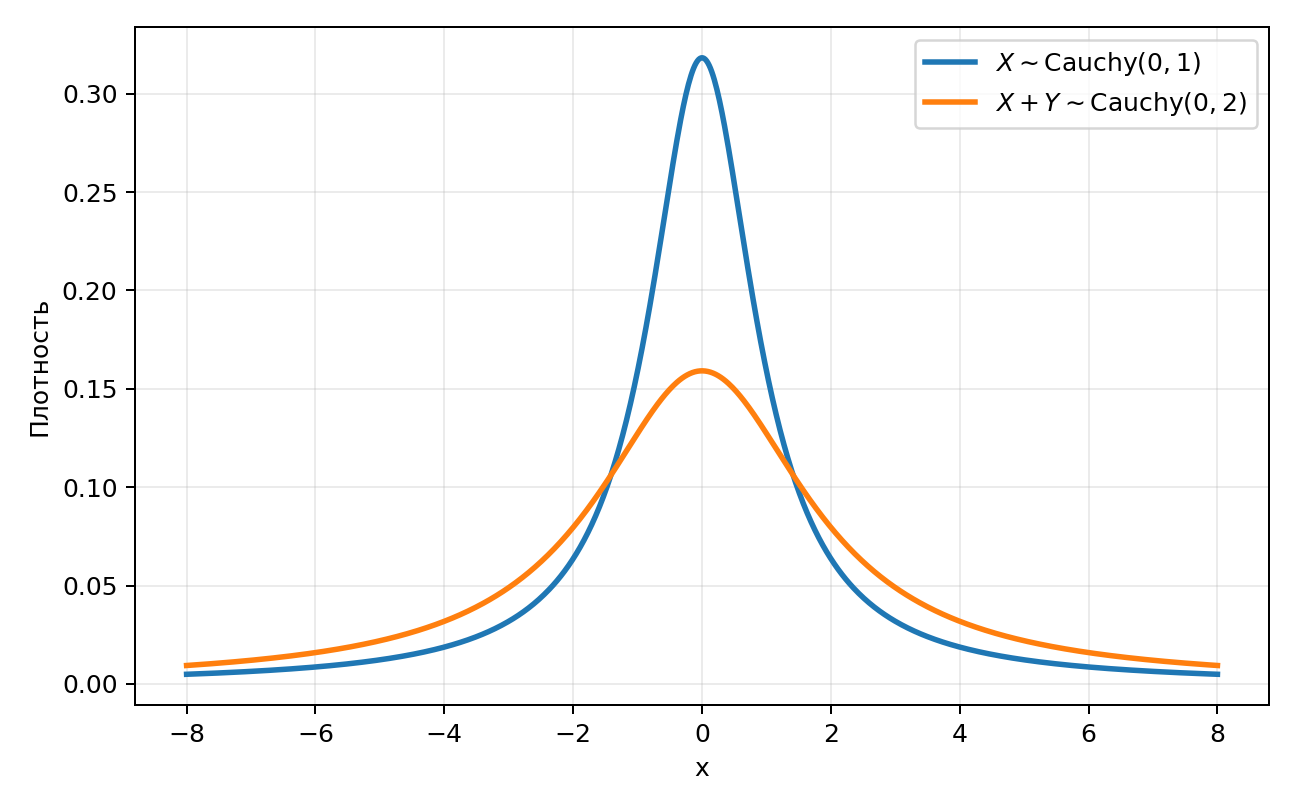
\includegraphics[width=0.74\linewidth,height=\textheight,keepaspectratio,alt={Сумма двух величин Коши}]{assets/figures/cauchy_sum.png}

\end{center}

\noindent\begin{minipage}[c]{\dimexpr\linewidth-30mm\relax}

\textbf{Интерактив}. \textbf{Сумма двух величин Коши}

В HTML-книге график строится из характеристических функций исходной
величины и её суммы с независимой копией.

\end{minipage}\hfill\begin{minipage}[c]{26mm}\centering

\href{https://neutrinohit.github.io/statistical-analysis-course/ru/book/chapters/03_characteristic_functions.html\#interactive-cauchy-sum}{
\includegraphics[width=24mm,height=\textheight,keepaspectratio,alt={QR-код интерактива}]{assets/qr/cauchy_sum.png}}

\end{minipage}

\end{semanticpdfbox}

У суммы максимум ниже, а распределение шире: параметр \(\gamma\)
увеличился с \(1\) до \(2\).

\subsection{Вычисление распределения суммы через
Фурье}\label{ux432ux44bux447ux438ux441ux43bux435ux43dux438ux435-ux440ux430ux441ux43fux440ux435ux434ux435ux43bux435ux43dux438ux44f-ux441ux443ux43cux43cux44b-ux447ux435ux440ux435ux437-ux444ux443ux440ux44cux435}

Весь метод состоит из трёх операций.

\begin{bookprocessflow}

\begin{bookprocessstep}[01]{Преобразовать плотности}

Найти характеристические функции

\begin{equation}\protect\phantomsection\label{eq-sum-fourier-step-forward}{
\varphi_X(t)=\int e^{itx}f_X(x)\,dx,
\qquad
\varphi_Y(t)=\int e^{ity}f_Y(y)\,dy.
}\end{equation}

\end{bookprocessstep}

\BookProcessConnector

\begin{bookprocessstep}[02]{Перемножить}

Для независимой суммы использовать

\begin{equation}\protect\phantomsection\label{eq-sum-fourier-step-product}{
\varphi_{X+Y}(t)=\varphi_X(t)\varphi_Y(t).
}\end{equation}

\end{bookprocessstep}

\BookProcessConnector

\begin{bookprocessstep}[03]{Вернуться к плотности}

Выполнить обратное преобразование

\begin{equation}\protect\phantomsection\label{eq-sum-fourier-step-inverse}{
f_{X+Y}(s)=
\frac{1}{2\pi}\int e^{-its}\varphi_{X+Y}(t)\,dt.
}\end{equation}

\end{bookprocessstep}

\end{bookprocessflow}

Для десяти слагаемых вместо девятикратной свёртки получается
произведение десяти функций и одно обратное преобразование.

\begin{booknote}

Тот же приём используется при восстановлении сигнала на фоне
независимого шума. Если \(D=S+N\), то \(\varphi_D=\varphi_S\varphi_N\).
Измерив шум отдельно, можно найти \(\varphi_S\) делением. На практике
это деление усиливает высокочастотные флуктуации и требует
регуляризации. Преобразование Фурье упрощает алгебру, но не улучшает
качество данных.

\end{booknote}

\section{Свойства характеристической
функции}\label{ux441ux432ux43eux439ux441ux442ux432ux430-ux445ux430ux440ux430ux43aux442ux435ux440ux438ux441ux442ux438ux447ux435ux441ux43aux43eux439-ux444ux443ux43dux43aux446ux438ux438}

\subsection{Дискретный
случай}\label{ux434ux438ux441ux43aux440ux435ux442ux43dux44bux439-ux441ux43bux443ux447ux430ux439}

Если \(X\) принимает значения \(x_k\) с вероятностями \(p_k\), интеграл
заменяется суммой:

\begin{equation}\protect\phantomsection\label{eq-characteristic-discrete}{
\varphi_X(t)=\sum_k p_k e^{itx_k}.
}\end{equation}

Это то же распределение, записанное в форме, удобной для сложения
случайных величин.

\subsection{Почему характеристическая функция всегда
существует}\label{ux43fux43eux447ux435ux43cux443-ux445ux430ux440ux430ux43aux442ux435ux440ux438ux441ux442ux438ux447ux435ux441ux43aux430ux44f-ux444ux443ux43dux43aux446ux438ux44f-ux432ux441ux435ux433ux434ux430-ux441ux443ux449ux435ux441ux442ux432ux443ux435ux442}

Модуль комплексной экспоненты равен единице. Поэтому

\begin{equation}\protect\phantomsection\label{eq-characteristic-bound}{
\left|\varphi_X(t)\right|
=\left|\mathbb E[e^{itX}]\right|
\leq \mathbb E[|e^{itX}|]
=1.
}\end{equation}

В отличие от математического ожидания \(\mathbb E[X]\) или дисперсии,
интеграл в определении характеристической функции не страдает от тяжёлых
хвостов: подынтегральная функция по модулю ограничена единицей.
Характеристическая функция существует у любого распределения.

\subsection{Базовые
свойства}\label{ux431ux430ux437ux43eux432ux44bux435-ux441ux432ux43eux439ux441ux442ux432ux430}

Для любой случайной величины выполняются соотношения

\begin{equation}\protect\phantomsection\label{eq-characteristic-basic-properties}{
\varphi_X(0)=1,
\qquad
|\varphi_X(t)|\leq1,
\qquad
\varphi_X(-t)=\varphi_X^*(t).
}\end{equation}

Первое равенство выражает нормировку вероятности:
\(\varphi_X(0)=\mathbb E[1]=1\). Третье следует из комплексного
сопряжения экспоненты. Для распределения, симметричного относительно
нуля, характеристическая функция вещественна и чётна.

\subsection{Сдвиг и
масштаб}\label{ux441ux434ux432ux438ux433-ux438-ux43cux430ux441ux448ux442ux430ux431}

Пусть \(Y=aX+b\). Тогда

\begin{equation}\protect\phantomsection\label{eq-characteristic-affine-transform}{
\begin{aligned}
\varphi_Y(t)
&=\mathbb E[e^{it(aX+b)}]\\
&=e^{itb}\mathbb E[e^{i(at)X}]\\
&=e^{itb}\varphi_X(at).
\end{aligned}
}\end{equation}

Сдвиг случайной величины даёт фазовый множитель, а изменение масштаба
меняет аргумент характеристической функции.

\section{Суммы многих независимых
величин}\label{ux441ux443ux43cux43cux44b-ux43cux43dux43eux433ux438ux445-ux43dux435ux437ux430ux432ux438ux441ux438ux43cux44bux445-ux432ux435ux43bux438ux447ux438ux43d}

Последовательно применяя формулу \ref{eq-characteristic-independent-sum}
к \(S_n=X_1+\dots+X_n\), получаем

\begin{equation}\protect\phantomsection\label{eq-characteristic-many-sum}{
\varphi_{S_n}(t)=
\prod_{k=1}^{n}\varphi_{X_k}(t).
}\end{equation}

Если все слагаемые имеют одно распределение,

\begin{equation}\protect\phantomsection\label{eq-characteristic-iid-sum}{
\varphi_{S_n}(t)=\left[\varphi_X(t)\right]^n.
}\end{equation}

Ради этих двух формул характеристические функции и вводят в задачах о
суммах.

\section{Примеры характеристических
функций}\label{ux43fux440ux438ux43cux435ux440ux44b-ux445ux430ux440ux430ux43aux442ux435ux440ux438ux441ux442ux438ux447ux435ux441ux43aux438ux445-ux444ux443ux43dux43aux446ux438ux439}

\subsection{Распределение
Бернулли}\label{ux440ux430ux441ux43fux440ux435ux434ux435ux43bux435ux43dux438ux435-ux431ux435ux440ux43dux443ux43bux43bux438}

Величина Бернулли принимает значение \(1\) с вероятностью \(p\) и
значение \(0\) с вероятностью \(1-p\). По формуле
\ref{eq-characteristic-discrete}

\begin{equation}\protect\phantomsection\label{eq-bernoulli-characteristic}{
\varphi_X(t)
=(1-p)e^{it\cdot0}+pe^{it\cdot1}
=(1-p)+pe^{it}.
}\end{equation}

Сумма \(S_n=X_1+\dots+X_n\) считает число единиц в \(n\) независимых
испытаниях. Её характеристическая функция равна

\begin{equation}\protect\phantomsection\label{eq-binomial-from-characteristic}{
\begin{aligned}
\varphi_{S_n}(t)
&=\left[(1-p)+pe^{it}\right]^n\\
&=\sum_{k=0}^{n}
\binom{n}{k}(1-p)^{n-k}p^k e^{itk}.
\end{aligned}
}\end{equation}

Коэффициент при \(e^{itk}\) равен вероятности \(P(S_n=k)\). Мы снова
получили биномиальное распределение:

\begin{equation}\protect\phantomsection\label{eq-binomial-distribution-from-bernoulli}{
P(S_n=k)=\binom{n}{k}p^k(1-p)^{n-k},
\qquad
S_n\sim\operatorname{Bin}(n,p).
}\end{equation}

Другого ответа и быть не могло: сумма нулей и единиц как раз считает
число успехов. Характеристическая функция показывает это непосредственно
в алгебраической форме.

\subsection{Распределение
Пуассона}\label{ux440ux430ux441ux43fux440ux435ux434ux435ux43bux435ux43dux438ux435-ux43fux443ux430ux441ux441ux43eux43dux430}

Для \(N\sim\operatorname{Pois}(\lambda)\)

\begin{equation}\protect\phantomsection\label{eq-poisson-characteristic}{
\begin{aligned}
\varphi_N(t)
&=\sum_{k=0}^{\infty}
e^{itk}e^{-\lambda}\frac{\lambda^k}{k!}\\
&=e^{-\lambda}
\sum_{k=0}^{\infty}\frac{(\lambda e^{it})^k}{k!}\\
&=\exp\!\left[\lambda(e^{it}-1)\right].
\end{aligned}
}\end{equation}

Пусть независимые величины \(N_k\) имеют параметры \(\lambda_k\). Тогда

\begin{equation}\protect\phantomsection\label{eq-poisson-sum-characteristic}{
\begin{aligned}
\varphi_{\sum_k N_k}(t)
&=\prod_k\exp\!\left[\lambda_k(e^{it}-1)\right]\\
&=\exp\!\left[
\left(\sum_k\lambda_k\right)(e^{it}-1)
\right].
\end{aligned}
}\end{equation}

Получилась характеристическая функция Пуассона с параметром
\(\sum_k\lambda_k\):

\begin{equation}\protect\phantomsection\label{eq-poisson-sum-distribution}{
\sum_k N_k
\sim
\operatorname{Pois}\!\left(\sum_k\lambda_k\right).
}\end{equation}

Это соответствует устройству опыта. Если несколько независимых
источников дают в среднем \(\lambda_1,\lambda_2,\ldots\) событий за один
интервал времени, общий счёт имеет среднее
\(\lambda_1+\lambda_2+\cdots\).

\subsection{Распределение
Гаусса}\label{ux440ux430ux441ux43fux440ux435ux434ux435ux43bux435ux43dux438ux435-ux433ux430ux443ux441ux441ux430}

Для \(X\sim\mathcal N(\mu,\sigma^2)\) характеристическая функция имеет
вид

\begin{equation}\protect\phantomsection\label{eq-normal-characteristic}{
\varphi_X(t)=
\exp\!\left(i\mu t-\frac{\sigma^2t^2}{2}\right).
}\end{equation}

\begin{bookderivation}

\subsubsection{Вывод характеристической функции
Гаусса}\label{ux432ux44bux432ux43eux434-ux445ux430ux440ux430ux43aux442ux435ux440ux438ux441ux442ux438ux447ux435ux441ux43aux43eux439-ux444ux443ux43dux43aux446ux438ux438-ux433ux430ux443ux441ux441ux430}

Сначала рассмотрим стандартную нормальную величину
\(Z\sim\mathcal N(0,1)\):

\begin{equation}\protect\phantomsection\label{eq-standard-normal-characteristic-integral}{
\varphi_Z(t)=
\frac{1}{\sqrt{2\pi}}
\int_{-\infty}^{+\infty}e^{itz}e^{-z^2/2}\,dz.
}\end{equation}

Продифференцируем по \(t\) и проинтегрируем по частям, используя
\(z e^{-z^2/2}=-d(e^{-z^2/2})/dz\):

\begin{equation}\protect\phantomsection\label{eq-standard-normal-characteristic-ode}{
\begin{aligned}
\varphi_Z'(t)
&=\frac{i}{\sqrt{2\pi}}
\int_{-\infty}^{+\infty}z e^{itz}e^{-z^2/2}\,dz\\
&=-t\varphi_Z(t).
\end{aligned}
}\end{equation}

Условие \(\varphi_Z(0)=1\) выбирает решение

\begin{equation}\protect\phantomsection\label{eq-standard-normal-characteristic}{
\varphi_Z(t)=e^{-t^2/2}.
}\end{equation}

Поскольку \(X=\mu+\sigma Z\), правило сдвига и масштаба
\ref{eq-characteristic-affine-transform} даёт формулу
\ref{eq-normal-characteristic}.

\end{bookderivation}

Для независимых \(X_k\sim\mathcal N(\mu_k,\sigma_k^2)\) произведение
характеристических функций равно

\begin{equation}\protect\phantomsection\label{eq-gaussian-sum-characteristic}{
\varphi_{\sum_k X_k}(t)=
\exp\!\left[
it\sum_k\mu_k-
\frac{t^2}{2}\sum_k\sigma_k^2
\right].
}\end{equation}

Это снова гауссова характеристическая функция. Следовательно,

\begin{equation}\protect\phantomsection\label{eq-gaussian-sum-distribution}{
\sum_k X_k
\sim
\mathcal N\!\left(
\sum_k\mu_k,
\sum_k\sigma_k^2
\right).
}\end{equation}

У независимых гауссовых величин складываются средние и дисперсии.
Стандартные отклонения складывать нельзя.

\subsection{Распределение
Коши}\label{ux440ux430ux441ux43fux440ux435ux434ux435ux43bux435ux43dux438ux435-ux43aux43eux448ux438}

Для независимых \(X_k\sim\operatorname{Cauchy}(0,1)\)

\begin{equation}\protect\phantomsection\label{eq-cauchy-many-sum-characteristic}{
\varphi_{S_n}(t)
=\left(e^{-|t|}\right)^n
=e^{-n|t|},
\qquad
S_n=\sum_{k=1}^{n}X_k.
}\end{equation}

Поэтому \(S_n\sim\operatorname{Cauchy}(0,n)\). После деления суммы на
\(n\) масштаб возвращается к единице:

\begin{equation}\protect\phantomsection\label{eq-cauchy-average-stability}{
\frac{S_n}{n}\sim\operatorname{Cauchy}(0,1).
}\end{equation}

Среднее арифметическое имеет то же распределение, что и каждое
слагаемое. Оно не сжимается с ростом \(n\). К этому примеру мы вернёмся
при обсуждении условий центральной предельной теоремы.

\section{Моменты из характеристической
функции}\label{ux43cux43eux43cux435ux43dux442ux44b-ux438ux437-ux445ux430ux440ux430ux43aux442ux435ux440ux438ux441ux442ux438ux447ux435ux441ux43aux43eux439-ux444ux443ux43dux43aux446ux438ux438}

Разложим комплексную экспоненту около \(t=0\):

\begin{equation}\protect\phantomsection\label{eq-complex-exponential-series}{
e^{itX}=\sum_{n=0}^{\infty}\frac{(itX)^n}{n!}.
}\end{equation}

Если соответствующие моменты существуют и разрешено переставить
математическое ожидание и сумму, то

\begin{equation}\protect\phantomsection\label{eq-characteristic-moment-expansion}{
\varphi_X(t)
=\sum_{n=0}^{\infty}
\frac{(it)^n}{n!}\mathbb E[X^n].
}\end{equation}

Отсюда моменты извлекаются производными в нуле:

\begin{equation}\protect\phantomsection\label{eq-moments-from-characteristic}{
\mathbb E[X^n]
=\frac{1}{i^n}\varphi_X^{(n)}(0).
}\end{equation}

В частности,

\begin{equation}\protect\phantomsection\label{eq-first-two-moments-from-characteristic}{
\mathbb E[X]=\frac{\varphi_X'(0)}{i},
\qquad
\mathbb E[X^2]=-\varphi_X''(0).
}\end{equation}

Слово «если» перед формулой \ref{eq-characteristic-moment-expansion}
нельзя выбрасывать. Сама характеристическая функция существует всегда,
её производные нужного порядка --- нет.

Для стандартного распределения Коши

\begin{equation}\protect\phantomsection\label{eq-cauchy-characteristic-at-zero}{
\varphi_X(t)=e^{-|t|}.
}\end{equation}

У этой функции нет производной при \(t=0\). Тот же факт виден в обычном
пространстве: интеграл для \(\mathbb E[X]\) не сходится абсолютно.
Односторонняя производная или главное значение интеграла не заменяют
математического ожидания.

\section{Кумулянты}\label{ux43aux443ux43cux443ux43bux44fux43dux442ux44b}

Произведение характеристических функций удобно превратить в сумму. Для
этого берётся логарифм:

\begin{equation}\protect\phantomsection\label{eq-cumulant-generating-function}{
K_X(t)=\ln\varphi_X(t).
}\end{equation}

Поскольку \(\varphi_X(0)=1\) и \(\varphi_X\) непрерывна, в некоторой
окрестности нуля она не обращается в нуль. Там можно выбрать непрерывную
ветвь логарифма с \(K_X(0)=0\). Если нужные производные существуют,
разложение имеет вид

\begin{equation}\protect\phantomsection\label{eq-cumulant-series}{
K_X(t)=
\sum_{n=1}^{\infty}
\kappa_n\frac{(it)^n}{n!},
}\end{equation}

а коэффициенты \(\kappa_n\) называются \textbf{кумулянтами}:

\begin{equation}\protect\phantomsection\label{eq-cumulants-from-characteristic}{
\kappa_n=
\frac{1}{i^n}
\left.
\frac{d^n}{dt^n}\ln\varphi_X(t)
\right|_{t=0}.
}\end{equation}

\subsection{Первые четыре
кумулянта}\label{ux43fux435ux440ux432ux44bux435-ux447ux435ux442ux44bux440ux435-ux43aux443ux43cux443ux43bux44fux43dux442ux430}

Для первой производной

\begin{equation}\protect\phantomsection\label{eq-first-cumulant-derivation}{
K_X'(0)=
\frac{\varphi_X'(0)}{\varphi_X(0)}
=i\mathbb E[X].
}\end{equation}

Для второй

\begin{equation}\protect\phantomsection\label{eq-second-cumulant-derivation}{
\begin{aligned}
K_X''(0)
&=\varphi_X''(0)-\left[\varphi_X'(0)\right]^2\\
&=-\mathbb E[X^2]+\mathbb E[X]^2\\
&=-\operatorname{Var}(X).
\end{aligned}
}\end{equation}

После деления на соответствующие степени \(i\) получаем

\begin{equation}\protect\phantomsection\label{eq-first-four-cumulants}{
\begin{aligned}
\kappa_1&=\mu,\\
\kappa_2&=\sigma^2,\\
\kappa_3&=\mathbb E[(X-\mu)^3],\\
\kappa_4&=\mathbb E[(X-\mu)^4]-3\sigma^4.
\end{aligned}
}\end{equation}

Первые два кумулянта --- среднее и дисперсия. Третий равен третьему
центральному моменту; после деления на \(\sigma^3\) он даёт коэффициент
асимметрии. Четвёртый измеряет отклонение четвёртого центрального
момента от гауссова значения \(3\sigma^4\); деление на \(\sigma^4\) даёт
эксцесс.

\subsection{Почему кумулянты удобны для
сумм}\label{ux43fux43eux447ux435ux43cux443-ux43aux443ux43cux443ux43bux44fux43dux442ux44b-ux443ux434ux43eux431ux43dux44b-ux434ux43bux44f-ux441ux443ux43cux43c}

Для независимых \(X\) и \(Y\)

\begin{equation}\protect\phantomsection\label{eq-cumulant-log-additivity}{
\begin{aligned}
K_{X+Y}(t)
&=\ln\!\left[\varphi_X(t)\varphi_Y(t)\right]\\
&=K_X(t)+K_Y(t).
\end{aligned}
}\end{equation}

Значит, каждый существующий кумулянт суммы равен сумме кумулянтов:

\begin{equation}\protect\phantomsection\label{eq-cumulant-additivity}{
\kappa_n(X+Y)=\kappa_n(X)+\kappa_n(Y).
}\end{equation}

Для изменения масштаба действует правило

\begin{equation}\protect\phantomsection\label{eq-cumulant-scaling}{
\kappa_n(aX)=a^n\kappa_n(X).
}\end{equation}

У обычных моментов суммы появляются смешанные члены. Кумулянты
независимых слагаемых складываются без таких членов, что особенно удобно
для нормированных сумм.

\section{Мост к центральной предельной
теореме}\label{ux43cux43eux441ux442-ux43a-ux446ux435ux43dux442ux440ux430ux43bux44cux43dux43eux439-ux43fux440ux435ux434ux435ux43bux44cux43dux43eux439-ux442ux435ux43eux440ux435ux43cux435}

Пусть \(X_1,\ldots,X_n\) независимы, имеют одно распределение и конечные
среднее и дисперсию:

\begin{equation}\protect\phantomsection\label{eq-clt-iid-moments}{
\mathbb E[X_k]=\mu,
\qquad
\operatorname{Var}(X_k)=\sigma^2<\infty.
}\end{equation}

Рассмотрим центрированную и нормированную сумму

\begin{equation}\protect\phantomsection\label{eq-clt-normalized-sum}{
Z_n=
\frac{1}{\sigma\sqrt n}
\sum_{k=1}^{n}(X_k-\mu).
}\end{equation}

Введём \(Y_k=(X_k-\mu)/\sigma\). Тогда \(\mathbb E[Y_k]=0\),
\(\operatorname{Var}(Y_k)=1\) и

\begin{equation}\protect\phantomsection\label{eq-clt-characteristic-sum}{
\varphi_{Z_n}(t)=
\left[
\varphi_Y\!\left(\frac{t}{\sqrt n}\right)
\right]^n.
}\end{equation}

Конечность второго момента даёт при \(u\to0\) разложение

\begin{equation}\protect\phantomsection\label{eq-clt-small-argument-expansion}{
\varphi_Y(u)=1-\frac{u^2}{2}+o(u^2).
}\end{equation}

Подставляя \(u=t/\sqrt n\), получаем

\begin{equation}\protect\phantomsection\label{eq-clt-characteristic-before-limit}{
\varphi_{Z_n}(t)=
\left[
1-\frac{t^2}{2n}+o\!\left(\frac1n\right)
\right]^n.
}\end{equation}

При каждом фиксированном \(t\)

\begin{equation}\protect\phantomsection\label{eq-clt-characteristic-limit}{
\lim_{n\to\infty}\varphi_{Z_n}(t)=e^{-t^2/2}.
}\end{equation}

Справа стоит характеристическая функция \(\mathcal N(0,1)\). Теорема
непрерывности Леви переводит сходимость характеристических функций в
сходимость по распределению {[}1{]}. Полную формулировку центральной
предельной теоремы и скорость приближения мы разберём в следующей главе.

Нормировка в формуле \ref{eq-clt-normalized-sum} обязательна. Сама сумма
имеет среднее \(n\mu\) и дисперсию \(n\sigma^2\); её центр и ширина
растут вместе с \(n\). Для среднего арифметического та же нормированная
величина записывается как

\begin{equation}\protect\phantomsection\label{eq-clt-normalized-sample-mean}{
Z_n=\frac{\overline X_n-\mu}{\sigma/\sqrt n}.
}\end{equation}

Отсюда возникает знакомый масштаб статистической неопределённости
среднего \(1/\sqrt n\).

\subsection{Тот же предел через
кумулянты}\label{ux442ux43eux442-ux436ux435-ux43fux440ux435ux434ux435ux43b-ux447ux435ux440ux435ux437-ux43aux443ux43cux443ux43bux44fux43dux442ux44b}

Если кумулянт порядка \(r\) существует, правила
\ref{eq-cumulant-additivity} и \ref{eq-cumulant-scaling} дают

\begin{equation}\protect\phantomsection\label{eq-clt-cumulant-scaling}{
\kappa_r(Z_n)=
n^{1-r/2}\kappa_r(Y).
}\end{equation}

При \(r=2\) дисперсия остаётся равной единице. Третий кумулянт убывает
как \(1/\sqrt n\), четвёртый --- как \(1/n\), а каждый существующий
кумулянт порядка \(r>2\) стремится к нулю. Если высшие кумулянты
существуют, в разложении остаётся квадратичный член
\(\ln\varphi(t)=-t^2/2\), соответствующий распределению Гаусса.

\section{Интерактив: приближение к распределению Гаусса в пространстве
Фурье}\label{interactive-clt-fourier}

Возьмём независимые величины

\begin{equation}\protect\phantomsection\label{eq-uniform-unit-variance}{
X_k\sim U(-\sqrt3,\sqrt3),
\qquad
\mathbb E[X_k]=0,
\qquad
\operatorname{Var}(X_k)=1.
}\end{equation}

На графике сравниваются характеристическая функция нормированной суммы и
предельная функция \(e^{-t^2/2}\). Ползунок меняет число слагаемых
\(n\).

\begin{semanticpdfbox}[breakable=false]

\begin{center}

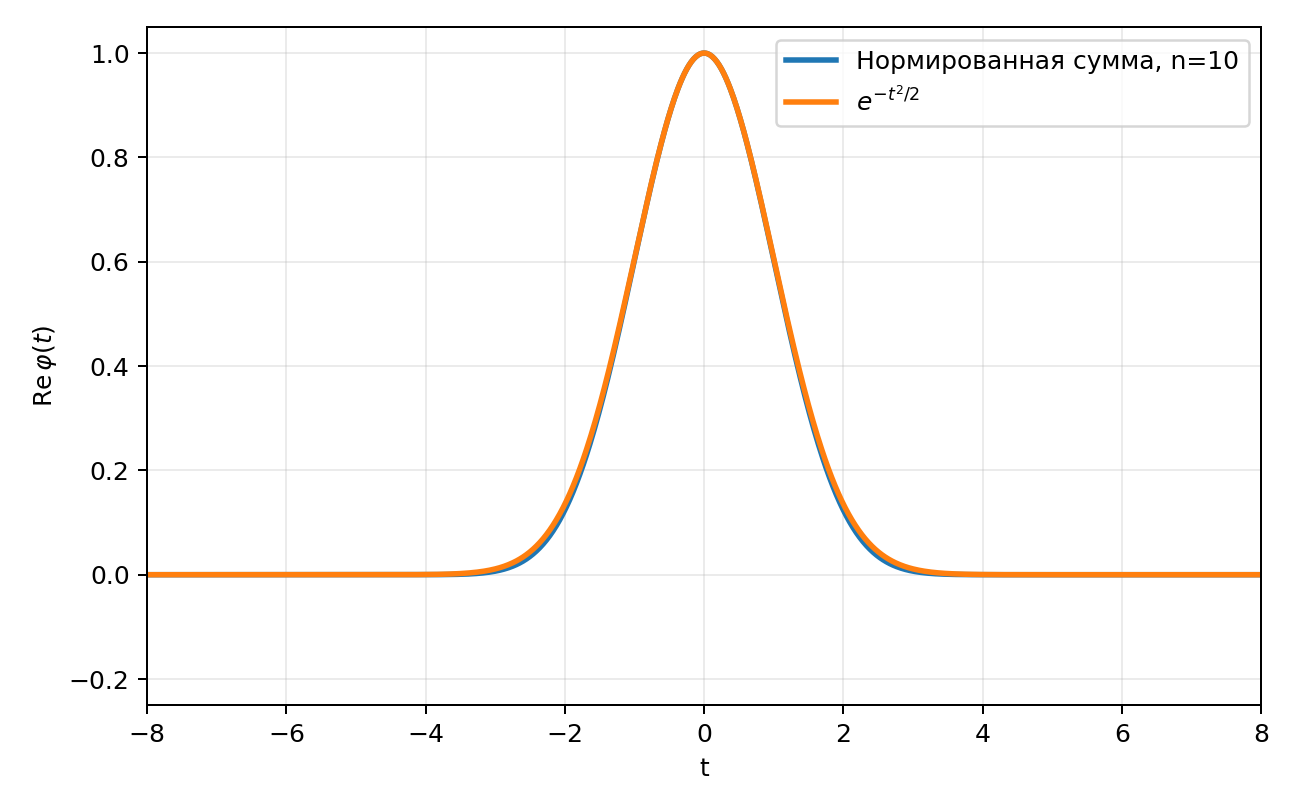
\includegraphics[width=0.74\linewidth,height=\textheight,keepaspectratio,alt={Гауссов предел в пространстве Фурье}]{assets/figures/clt_fourier_n10.png}

\end{center}

\noindent\begin{minipage}[c]{\dimexpr\linewidth-30mm\relax}

\textbf{Интерактив}. \textbf{Гауссов предел в пространстве Фурье}

Меняя число слагаемых, можно проследить, как характеристическая функция
нормированной суммы приближается к \(e^{-t^2/2}\).

\end{minipage}\hfill\begin{minipage}[c]{26mm}\centering

\href{https://neutrinohit.github.io/statistical-analysis-course/ru/book/chapters/03_characteristic_functions.html\#interactive-clt-fourier}{
\includegraphics[width=24mm,height=\textheight,keepaspectratio,alt={QR-код интерактива}]{assets/qr/clt_fourier.png}}

\end{minipage}

\end{semanticpdfbox}

\begin{bookchaptersummary}[Итоги главы]

\begin{itemize}
\tightlist
\item
  Характеристическая функция является преобразованием Фурье
  распределения и существует для любой случайной величины.
\item
  Для суммы независимых величин характеристические функции
  перемножаются. Это заменяет последовательные свёртки плотностей
  обычным произведением.
\item
  Моменты связаны с производными \(\varphi_X(t)\) в нуле, а кумулянты
  --- с производными \(\ln\varphi_X(t)\). Характеристическая функция
  существует всегда; нужных производных у неё может не быть.
\item
  У нормированной суммы сохраняется дисперсия, а вклад высших
  существующих кумулянтов убывает с ростом числа слагаемых. Так
  характеристические функции приводят к гауссову пределу.
\end{itemize}

\end{bookchaptersummary}

\section{Задачи}\label{ux437ux430ux434ux430ux447ux438-2}

\begin{semanticpdfbox}[colback=BookCoralSoft,borderline west={1.2mm}{0pt}{BookCoral},breakable=false]

\noindent{\sffamily\bfseries\fontsize{11.2}{13.5}\selectfont Задача 1. Сумма двух равномерных величин}\par\nopagebreak[4]\vspace{1.2mm}

Пусть независимые случайные величины распределены равномерно: \[
X,Y\sim\mathrm{U}(0,1),
\qquad
f_X(x)=f_Y(x)=\theta(x)\theta(1-x).
\]

Для суммы \(S=X+Y\):

\begin{enumerate}
\def\labelenumi{\arabic{enumi}.}
\tightlist
\item
  Вычислите плотность \(f_S(s)\) непосредственно как свёртку.
\item
  Покажите, что произведение \(\theta\)-функций ограничивает область
  интегрирования условием \[
  \max(0,s-1)\le x\le\min(1,s).
  \]
\item
  Получите кусочно заданную треугольную плотность и проверьте её
  нормировку.
\item
  Найдите характеристическую функцию \(\varphi_X(t)\).
\item
  Используя \(\varphi_S(t)=\varphi_X(t)^2\), получите тот же ответ через
  обратное преобразование Фурье.
\item
  Нарисуйте плотности \(f_X(x)\) и \(f_S(s)\) и объясните форму
  распределения суммы.
\end{enumerate}

\end{semanticpdfbox}

\begin{semanticpdfbox}[colback=BookCoralSoft,borderline west={1.2mm}{0pt}{BookCoral},breakable=false]

\noindent{\sffamily\bfseries\fontsize{11.2}{13.5}\selectfont Задача 2. Распределение Бернулли}\par\nopagebreak[4]\vspace{1.2mm}

Пусть \[
P(X=1)=p,\qquad P(X=0)=1-p.
\]

\begin{enumerate}
\def\labelenumi{\arabic{enumi}.}
\tightlist
\item
  Найдите \(\varphi_X(t)\).
\item
  Найдите характеристическую функцию суммы \(n\) независимых величин
  Бернулли.
\item
  Объясните, почему сумма имеет биномиальное распределение.
\end{enumerate}

\end{semanticpdfbox}

\begin{semanticpdfbox}[colback=BookCoralSoft,borderline west={1.2mm}{0pt}{BookCoral},breakable=false]

\noindent{\sffamily\bfseries\fontsize{11.2}{13.5}\selectfont Задача 3. Сумма пуассоновских величин}\par\nopagebreak[4]\vspace{1.2mm}

Для независимых \[
N_1\sim\mathrm{Pois}(\lambda_1),\qquad
N_2\sim\mathrm{Pois}(\lambda_2)
\] покажите с помощью характеристических функций, что \[
N_1+N_2\sim\mathrm{Pois}(\lambda_1+\lambda_2).
\]

\end{semanticpdfbox}

\begin{semanticpdfbox}[colback=BookCoralSoft,borderline west={1.2mm}{0pt}{BookCoral},breakable=false]

\noindent{\sffamily\bfseries\fontsize{11.2}{13.5}\selectfont Задача 4. Сумма гауссовых величин}\par\nopagebreak[4]\vspace{1.2mm}

Пусть независимые величины распределены как \[
X_k\sim\mathrm{N}(\mu_k,\sigma_k^2).
\] Покажите, что \[
\sum_kX_k
\sim
\mathrm{N}\!\left(\sum_k\mu_k,\sum_k\sigma_k^2\right).
\]

\end{semanticpdfbox}

\begin{semanticpdfbox}[colback=BookCoralSoft,borderline west={1.2mm}{0pt}{BookCoral},breakable=false]

\noindent{\sffamily\bfseries\fontsize{11.2}{13.5}\selectfont Задача 5. Моменты и производные}\par\nopagebreak[4]\vspace{1.2mm}

Для \[
\varphi_N(t)=\exp\!\left[\lambda(e^{it}-1)\right]
\] найдите \(\mathbb{E}[N]\), \(\mathbb{E}[N^2]\) и \(\mathrm{Var}(N)\)
через производные в нуле.

\end{semanticpdfbox}

\begin{semanticpdfbox}[colback=BookCoralSoft,borderline west={1.2mm}{0pt}{BookCoral},breakable=false]

\noindent{\sffamily\bfseries\fontsize{11.2}{13.5}\selectfont Задача 6. Распределение Коши}\par\nopagebreak[4]\vspace{1.2mm}

Для \[
\varphi_X(t)=e^{-|t|}
\] объясните, почему \(\varphi_X'(0)\) не существует, и покажите, что \[
\frac{X_1+\dots+X_n}{n}
\] имеет то же распределение Коши.

\end{semanticpdfbox}

\begin{semanticpdfbox}[colback=BookCoralSoft,borderline west={1.2mm}{0pt}{BookCoral},breakable=false]

\noindent{\sffamily\bfseries\fontsize{11.2}{13.5}\selectfont Задача 7. Распределение \(S_n=X_1+\dots+X_n\) в пределе \(n\to\infty\)}\par\nopagebreak[4]\vspace{1.2mm}

Пусть \(X_1,\dots,X_n\) --- независимые одинаково распределённые
случайные величины, \[
S_n=X_1+\dots+X_n,
\qquad
\langle X\rangle_n=\frac{S_n}{n}.
\]

Среднее и вариация \(X_i\): \[
\mathbb{E}[X_i]=\mu,
\qquad
\mathrm{Var}(X_i)=\sigma^2<\infty.
\] Рассмотрим нормированную сумму \[
Z_n=
\frac{S_n-n\mu}{\sigma\sqrt n}.
\]

\begin{itemize}
\item
  Покажите, что характеристическая функция \(Z_n\) имеет вид \[
   \varphi_{Z_n}(t) =
   \left[
   e^{-it\mu/(\sigma\sqrt n)}
   \varphi_X\left(\frac{t}{\sigma\sqrt n}\right)
   \right]^n.
   \]
\item
  Для каждого из следующих распределений найдите характеристическую
  функцию и предел \[
   \lim_{n\to\infty}\varphi_{Z_n}(t).
   \]

  \textbf{Симметричное распределение Бернулли:} \[
   P(X=1)=P(X=-1)=\frac12.
   \]

  \textbf{Равномерное распределение:} \[
   X\sim U(-\sqrt3,\sqrt3).
   \]

  \textbf{Экспоненциальное распределение:} \[
   X\sim \mathrm{Exp}(1).
   \]

  \textbf{Распределение Пуассона:} \[
   X\sim \mathrm{Pois}(\lambda).
   \]
\item
  Убедитесь, что во всех четырёх случаях получается один и тот же
  предел: \[
   \varphi_{Z_n}(t)\to e^{-t^2/2}.
   \]
\end{itemize}

\end{semanticpdfbox}

\section*{Литература}\label{ux43bux438ux442ux435ux440ux430ux442ux443ux440ux430-2}
\addcontentsline{toc}{section}{Литература}

\markright{Литература}

\protect\phantomsection\label{refs}
\begin{CSLReferences}{0}{0}
\bibitem[\citeproctext]{ref-feller1971}
{[}1{]} Feller, W. \emph{An Introduction to Probability Theory and Its
Applications}. John Wiley \& Sons. 1971.

\end{CSLReferences}

\chapter{Центральная предельная теорема и нормальное
распределение}\label{ux446ux435ux43dux442ux440ux430ux43bux44cux43dux430ux44f-ux43fux440ux435ux434ux435ux43bux44cux43dux430ux44f-ux442ux435ux43eux440ux435ux43cux430-ux438-ux43dux43eux440ux43cux430ux43bux44cux43dux43eux435-ux440ux430ux441ux43fux440ux435ux434ux435ux43bux435ux43dux438ux435}

\bookchapteropeningcontents

\begin{bookchapteropening}[Аннотация]

Центральная предельная теорема - одна из важнейших теорем в
статистическом анализе. Она показывает фундаментально важную роль
нормального распределения. Мы увидим как нормальное или гауссовое
распределение возникает почти волшебным образом для описания суммы
бесконечного количества случайных величин. Причём каждая из них может
следовать почти любому распределению. Мы выведем среднее и дисперсию
суммы, разберём точную формулировку теоремы и проследим гауссов предел в
численном эксперименте. Нормальное распределение затем станет рабочим
инструментом: через его квантили мы построим центральные области и
сравним два независимых измерения.

\end{bookchapteropening}

\section{Физическая задача: сигнал
фотодетектора}\label{ux444ux438ux437ux438ux447ux435ux441ux43aux430ux44f-ux437ux430ux434ux430ux447ux430-ux441ux438ux433ux43dux430ux43b-ux444ux43eux442ux43eux434ux435ux442ux435ux43aux442ux43eux440ux430}

Пусть короткая вспышка света выбивает в фотодетекторе \(N\)
фотоэлектронов. Каждый фотоэлектрон создаёт на выходе электрический
импульс со случайным зарядом \(Q_i\). Электроника измеряет их сумму

\begin{equation}\protect\phantomsection\label{eq-photodetector-charge-sum}{
Q_N=Q_1+Q_2+\cdots+Q_N.
}\end{equation}

Даже при одинаковых вспышках заряды отдельных импульсов немного
различаются. Обозначим средний заряд одного импульса через \(q_0\), а
его дисперсию --- через \(s_q^2\):

\begin{equation}\protect\phantomsection\label{eq-single-photoelectron-moments}{
\mathbb E[Q_i]=q_0,
\qquad
\operatorname{Var}(Q_i)=s_q^2.
}\end{equation}

В простейшей модели импульсы независимы и подчиняются одному
распределению. Тогда

\begin{equation}\protect\phantomsection\label{eq-photodetector-charge-moments}{
\mathbb E[Q_N]=Nq_0,
\qquad
\operatorname{Var}(Q_N)=Ns_q^2.
}\end{equation}

Средний сигнал растёт как \(N\), его стандартное отклонение --- как
\(\sqrt N\). Относительная ширина пика равна

\begin{equation}\protect\phantomsection\label{eq-photodetector-relative-resolution}{
\frac{\sigma_{Q_N}}{\mathbb E[Q_N]}
=
\frac{s_q}{q_0\sqrt N}.
}\end{equation}

Если среднее число фотоэлектронов пропорционально энергии, этот
результат даёт знакомый стохастический вклад в энергетическое
разрешение, пропорциональный \(1/\sqrt E\). Остаётся понять форму пика.
Центральная предельная теорема даёт ответ:

\begin{equation}\protect\phantomsection\label{eq-photodetector-gaussian-limit}{
\frac{Q_N-Nq_0}{s_q\sqrt N}
\ \xrightarrow[N\to\infty]{d}\
\mathcal N(0,1).
}\end{equation}

Вся задача уложилась в среднее суммы, дисперсию суммы и одну предельную
теорему. В реальном детекторе флуктуирует также число фотоэлектронов,
бывают корреляции, неоднородности и шум электроники. Они меняют
коэффициент и добавляют другие слагаемые к разрешению. Упрощённая модель
показывает сам механизм: средние независимых вкладов складываются, и их
дисперсии тоже складываются.

Теперь разберём этот расчёт по частям.

\section{Псевдослучайные числа}\label{interactive-uniform-sample}

Для проверки центральной предельной теоремы устроим численный
эксперимент. В первой главе мы уже генерировали псевдоданные и подбирали
ширину распределения. Откуда компьютер берёт случайные числа?

Он этого не умеет делать! Любой генератор случайных чисел генерирует
последовательность псевдослучайных чисел, потому что его программа
представляет собой детерминированный алгоритм. Внутреннее состояние
генератора полностью определяет следующее число. При удачно выбранном
алгоритме последовательность проходит статистические тесты и имеет
период, намного превышающий длину обычного расчёта. Для моделирования
этого достаточно, хотя физического источника случайности внутри
алгоритма нет.

Начальное состояние генератора задаётся некоторым \emph{начальным}
числом, по английски \emph{seed}. Одинаковое начальное состояние
воспроизводит ту же последовательность. Это удобно при проверке
программы: рисунок или численный результат можно получить ещё раз.

Генератор равномерного распределения на \([-1,1]\) в NumPy вызывается
несколькими строками:

\begin{Shaded}
\begin{Highlighting}[]
\ImportTok{import}\NormalTok{ numpy }\ImportTok{as}\NormalTok{ np}

\NormalTok{rng }\OperatorTok{=}\NormalTok{ np.random.default\_rng(}\DecValTok{7}\NormalTok{)}
\NormalTok{x }\OperatorTok{=}\NormalTok{ rng.uniform(}\OperatorTok{{-}}\DecValTok{1}\NormalTok{, }\DecValTok{1}\NormalTok{, size}\OperatorTok{=}\DecValTok{20\_000}\NormalTok{)}
\end{Highlighting}
\end{Shaded}

На рисунке \ref{fig-uniform-pseudorandom-sample} показана гистограмма
такой выборки. Отдельные числа ничего не сообщают о форме распределения.
На большой выборке становится видна постоянная плотность \(f(x)=1/2\)
внутри заданного интервала.

\begin{figure}

\centering{

\pandocbounded{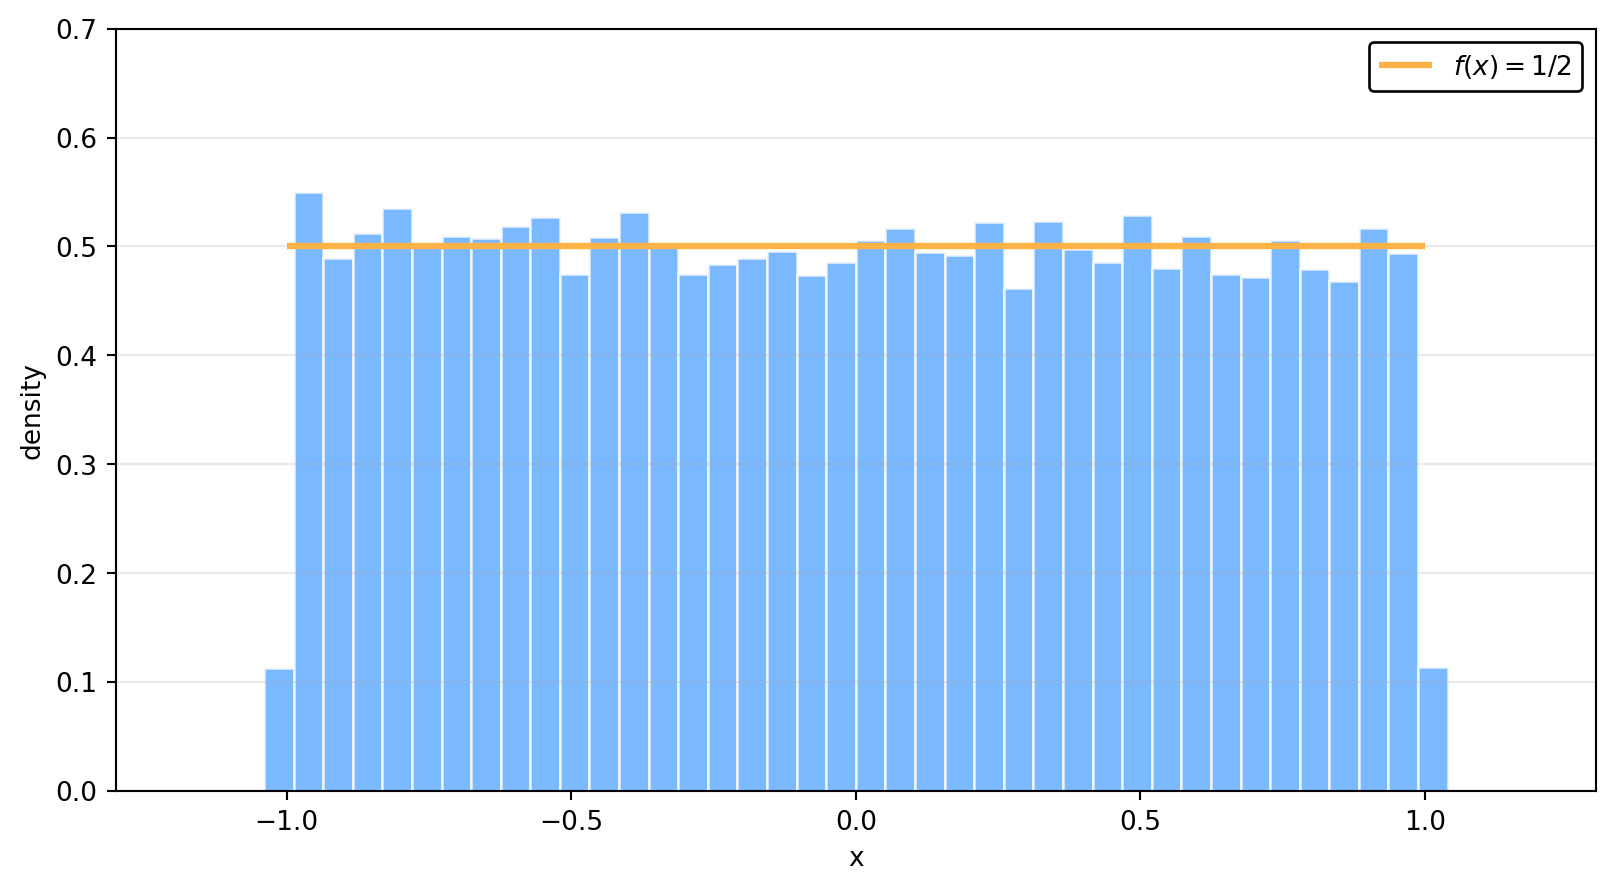
\includegraphics[keepaspectratio]{chapters/../assets/figures/clt_uniform_sample.png}}

}

\caption{\label{fig-uniform-pseudorandom-sample}Гистограмма 20 000
псевдослучайных чисел, равномерно распределённых на \([-1,1]\);
горизонтальная линия показывает плотность \(f(x)=1/2\)}

\end{figure}%

Гистограмма сама остаётся случайной: при другом начальном состоянии
высоты столбцов изменятся. Распределение и его параметры при этом заданы
в программе и остаются теми же.

\section{Среднее и дисперсия
суммы}\label{ux441ux440ux435ux434ux43dux435ux435-ux438-ux434ux438ux441ux43fux435ux440ux441ux438ux44f-ux441ux443ux43cux43cux44b}

Рассмотрим сумму \(m\) случайных величин

\begin{equation}\protect\phantomsection\label{eq-random-sum-definition}{
S_m=X_1+X_2+\cdots+X_m.
}\end{equation}

Математическое ожидание линейно:

\begin{equation}\protect\phantomsection\label{eq-random-sum-mean}{
\mathbb E[S_m]
=\sum_{i=1}^{m}\mathbb E[X_i].
}\end{equation}

Для этого равенства независимость не требуется. Со средним всё
складывается буквально. При вычислении дисперсии появляются произведения
разных слагаемых. Их описывает ковариация.

\begin{booknote}

\textbf{Ковариация} случайных величин \(X\) и \(Y\) определяется
равенством

\begin{equation}\protect\phantomsection\label{eq-covariance-definition-clt}{
\begin{aligned}
\operatorname{cov}(X,Y)
&=\mathbb E\!\left[
(X-\mathbb E[X])(Y-\mathbb E[Y])
\right]\\
&=\mathbb E[XY]-\mathbb E[X]\mathbb E[Y].
\end{aligned}
}\end{equation}

При \(X=Y\) ковариация превращается в дисперсию:
\(\operatorname{cov}(X,X)=\operatorname{Var}(X)\).

\end{booknote}

\begin{bookderivation}

\subsection{Дисперсия
суммы}\label{ux434ux438ux441ux43fux435ux440ux441ux438ux44f-ux441ux443ux43cux43cux44b}

Вычтем из каждого слагаемого его среднее и раскроем квадрат:

\begin{equation}\protect\phantomsection\label{eq-random-sum-variance-general}{
\begin{aligned}
\operatorname{Var}(S_m)
&=\mathbb E\!\left[
\left(\sum_{i=1}^{m}(X_i-\mathbb E[X_i])\right)^2
\right]\\
&=\sum_{i=1}^{m}\operatorname{Var}(X_i)
+2\sum_{i<j}\operatorname{cov}(X_i,X_j).
\end{aligned}
}\end{equation}

Для независимых величин
\(\mathbb E[X_iX_j]=\mathbb E[X_i]\mathbb E[X_j]\) при \(i\ne j\),
поэтому все ковариации в двойной сумме равны нулю:

\begin{equation}\protect\phantomsection\label{eq-independent-sum-variance}{
\operatorname{Var}(S_m)
=\sum_{i=1}^{m}\operatorname{Var}(X_i).
}\end{equation}

\end{bookderivation}

Результат из уравнения \ref{eq-independent-sum-variance} мы уже
использовали для фотодетектора. Стандартные отклонения независимых
вкладов складываются в квадратуре. Если между вкладами есть корреляции,
двойная сумма в уравнении \ref{eq-random-sum-variance-general}
сохраняется.

\subsection{Равномерные
слагаемые}\label{ux440ux430ux432ux43dux43eux43cux435ux440ux43dux44bux435-ux441ux43bux430ux433ux430ux435ux43cux44bux435}

Для численного эксперимента возьмём независимые одинаково распределённые
величины

\begin{equation}\protect\phantomsection\label{eq-uniform-summands}{
X_i\sim U(-1,1).
}\end{equation}

Симметрия даёт \(\mathbb E[X_i]=0\). Плотность равна \(1/2\) на
\([-1,1]\), поэтому

\begin{equation}\protect\phantomsection\label{eq-uniform-summand-moments}{
\begin{aligned}
\mathbb E[X_i^2]
&=\frac12\int_{-1}^{1}x^2\,dx=\frac13,\\
\operatorname{Var}(X_i)
&=\mathbb E[X_i^2]-\mathbb E[X_i]^2=\frac13.
\end{aligned}
}\end{equation}

Для суммы \(S_m\) получаем

\begin{equation}\protect\phantomsection\label{eq-uniform-sum-moments}{
\mathbb E[S_m]=0,
\qquad
\operatorname{Var}(S_m)=\frac m3.
}\end{equation}

Ширина самой суммы растёт с \(m\). Чтобы сравнивать её форму при разных
\(m\), нужно каждый раз вернуть среднее к нулю, а дисперсию --- к
единице:

\begin{equation}\protect\phantomsection\label{eq-uniform-normalized-sum}{
Z_m=\frac{S_m}{\sqrt{m/3}}
=\frac{X_1+\cdots+X_m}{\sqrt{m/3}}.
}\end{equation}

\section{Центральная предельная
теорема}\label{ux446ux435ux43dux442ux440ux430ux43bux44cux43dux430ux44f-ux43fux440ux435ux434ux435ux43bux44cux43dux430ux44f-ux442ux435ux43eux440ux435ux43cux430}

Теперь можно сформулировать теорему без сокращений.

\begin{booknote}

\textbf{Центральная предельная теорема.} Пусть \(X_1,\ldots,X_m\)
независимы, одинаково распределены и имеют конечные среднее и ненулевую
дисперсию:

\[
\mathbb E[X_i]=\mu,
\qquad
0<\operatorname{Var}(X_i)=\sigma^2<\infty.
\]

Тогда

\begin{equation}\protect\phantomsection\label{eq-central-limit-theorem-iid}{
Z_m=
\frac{\displaystyle\sum_{i=1}^{m}X_i-m\mu}
{\sigma\sqrt m}
\xrightarrow[m\to\infty]{d}
\mathcal N(0,1).
}\end{equation}

\end{booknote}

Стрелка \(\xrightarrow{d}\) означает сходимость по распределению. При
каждом фиксированном \(z\) в точке непрерывности предельной функции
распределения

\[
P(Z_m\le z)\longrightarrow \Phi(z),
\]

где \(\Phi\) --- CDF стандартного нормального распределения. В
предыдущей главе мы увидели тот же предел через характеристические
функции.

Для независимых, но неодинаково распределённых слагаемых одной
конечности дисперсий мало. Один член суммы может сохранить заметную долю
полного разброса и определять форму результата. Условия Линдеберга и
Ляпунова исключают такое доминирование; соответствующие варианты теоремы
приведены, например, в {[}1{]}.

\begin{semanticpdfbox}[colback=BookBiographySoft,borderline west={1.2mm}{0pt}{BookBiography},breakable=false]

\noindent\begin{minipage}[t]{30mm}\vspace{0pt}\centering

\href{https://mathshistory.st-andrews.ac.uk/Biographies/Lyapunov/pictdisplay/}{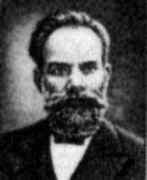
\includegraphics[width=28mm,height=\textheight,keepaspectratio,alt={Портрет Александра Михайловича Ляпунова}]{assets/people/aleksandr-lyapunov.jpg}}

\end{minipage}\hfill\begin{minipage}[t]{\dimexpr\linewidth-35mm\relax}\vspace{0pt}

{\sffamily\bfseries\footnotesize\color{BookBiography} БИОГРАФИЯ\par}\vspace{0.8mm}{\sffamily\bfseries\large\color{BookInk} Александр Михайлович Ляпунов\par}

{\sffamily\small\color{BookMuted} 1857–1918\par}\vspace{1.4mm}

Русский математик, известный работами по устойчивости движения и теории
вероятностей. В начале XX века Ляпунов доказал вариант центральной
предельной теоремы методом характеристических функций. Условие,
названное его именем, ограничивает вклад далёких значений отдельных
слагаемых.

{\footnotesize\color{BookMuted}

\textbf{Источник:}
\href{https://mathshistory.st-andrews.ac.uk/Biographies/Lyapunov/}{MacTutor};
фото
\href{https://mathshistory.st-andrews.ac.uk/Biographies/Lyapunov/pictdisplay/}{MacTutor}

}

\end{minipage}

\end{semanticpdfbox}

В формуле \ref{eq-central-limit-theorem-iid} существенны центрирование и
нормировка. Среднее ненормированной суммы равно \(m\mu\), а стандартное
отклонение --- \(\sigma\sqrt m\). И центр, и ширина уходят с ростом
\(m\). Для выборочного среднего \(\overline X_m=S_m/m\) та же
нормированная величина имеет вид

\begin{equation}\protect\phantomsection\label{eq-clt-sample-mean}{
Z_m=
\frac{\overline X_m-\mu}{\sigma/\sqrt m}.
}\end{equation}

Отсюда появляется масштаб статистической неопределённости среднего
\(\sigma/\sqrt m\).

Теорема описывает распределение результатов повторяемого опыта. Она
ничего не обещает отдельной реализации \(Z_m\): значения порядка двух
или трёх стандартных отклонений сохраняют ненулевую вероятность и при
сколь угодно большом \(m\).

Универсального числа слагаемых, после которого разрешается написать
«распределение уже гауссово», тоже нет. Если существует третий
абсолютный центральный момент

\[
\rho_3=\mathbb E\!\left[|X_i-\mu|^3\right],
\]

неравенство Берри---Эссеена даёт оценку

\begin{equation}\protect\phantomsection\label{eq-berry-esseen-bound}{
\sup_z
\left|P(Z_m\le z)-\Phi(z)\right|
\le
C\frac{\rho_3}{\sigma^3\sqrt m},
}\end{equation}

где \(C\) --- универсальная константа. Отношение \(\rho_3/\sigma^3\)
зависит от исходного распределения. Кроме того, малая абсолютная ошибка
CDF может быть заметной относительной ошибкой в далёком хвосте. При
поиске редких сигналов проверка гауссова приближения в центральной
области ещё не решает задачу для хвостовой вероятности.

\subsection{Как меняется форма суммы}\label{interactive-clt-sums}

Для равномерных слагаемых из уравнения \ref{eq-uniform-summands} при
\(m=1\) распределение остаётся равномерным. При \(m=2\) свёртка двух
прямоугольников даёт треугольник. Дальше углы сглаживаются, и
распределение нормированной суммы приближается к стандартному гауссу.

\begin{semanticpdfbox}[breakable=false]

\begin{center}

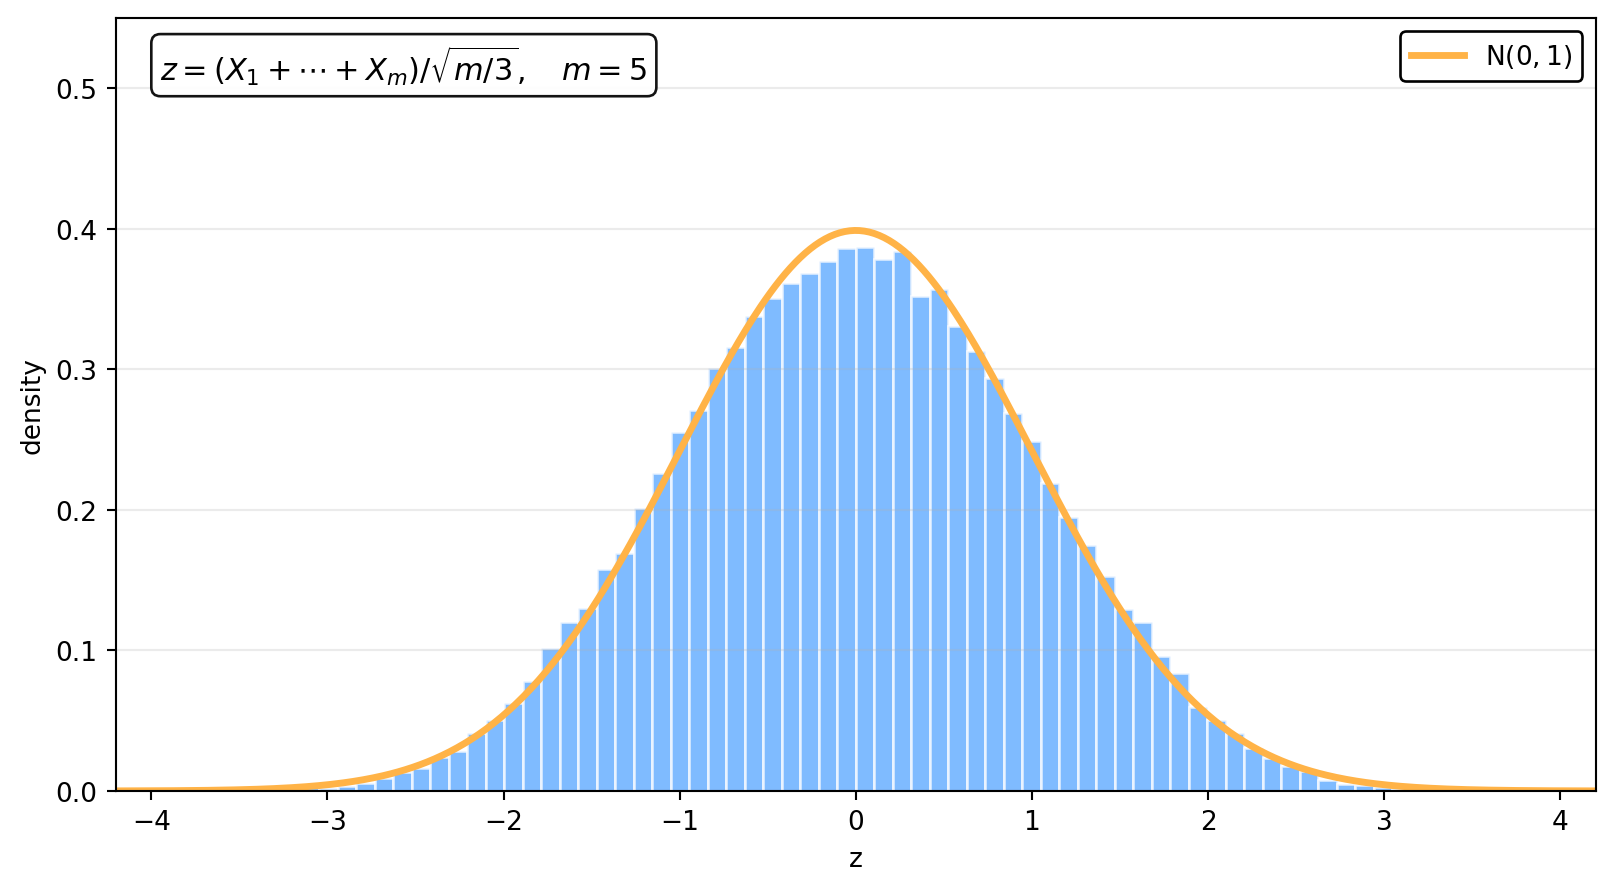
\includegraphics[width=0.74\linewidth,height=\textheight,keepaspectratio,alt={Форма нормированной суммы}]{assets/figures/clt_uniform_sum_m5.png}

\end{center}

\noindent\begin{minipage}[c]{\dimexpr\linewidth-30mm\relax}

\textbf{Интерактив}. \textbf{Форма нормированной суммы}

Меняйте число слагаемых и объём выборки. Гистограмма показывает новую
реализацию численного эксперимента, а гладкая кривая --- плотность
\(\mathcal N(0,1)\).

\end{minipage}\hfill\begin{minipage}[c]{26mm}\centering

\href{https://neutrinohit.github.io/statistical-analysis-course/ru/book/chapters/04_central_limit_theorem.html\#interactive-clt-sums}{
\includegraphics[width=24mm,height=\textheight,keepaspectratio,alt={QR-код интерактива}]{assets/qr/clt_sums.png}}

\end{minipage}

\end{semanticpdfbox}

Вернёмся к фотодетектору. Формула \ref{eq-photodetector-gaussian-limit}
является прямым применением ЦПТ к зарядам однофотоэлектронных импульсов.
Гауссова форма пика и закон \(1/\sqrt N\) имеют одно происхождение.
Первое относится к форме распределения нормированной суммы, второе --- к
её относительной ширине.

\section{Нормальное
распределение}\label{ux43dux43eux440ux43cux430ux43bux44cux43dux43eux435-ux440ux430ux441ux43fux440ux435ux434ux435ux43bux435ux43dux438ux435}

Нормальное, или гауссово, распределение уже появлялось в главах 2 и 3.
Здесь оно нужно как числовая шкала отклонений.

Случайная величина \(X\sim\mathcal N(\mu,\sigma^2)\) имеет плотность

\begin{equation}\protect\phantomsection\label{eq-clt-normal-density}{
f(x;\mu,\sigma)=
\frac{1}{\sigma\sqrt{2\pi}}
\exp\!\left[-\frac{(x-\mu)^2}{2\sigma^2}\right],
\qquad \sigma>0.
}\end{equation}

Плотность достигает максимума при \(x=\mu\), математическое ожидание
равно \(\mu\), а дисперсия --- \(\sigma^2\). В записи
\(\mathcal N(\mu,\sigma^2)\) вторым параметром стоит именно дисперсия.

На рисунке \ref{fig-standard-normal-density} показана плотность при
\(\mu=0\) и \(\sigma=1\).

\begin{figure}

\centering{

\pandocbounded{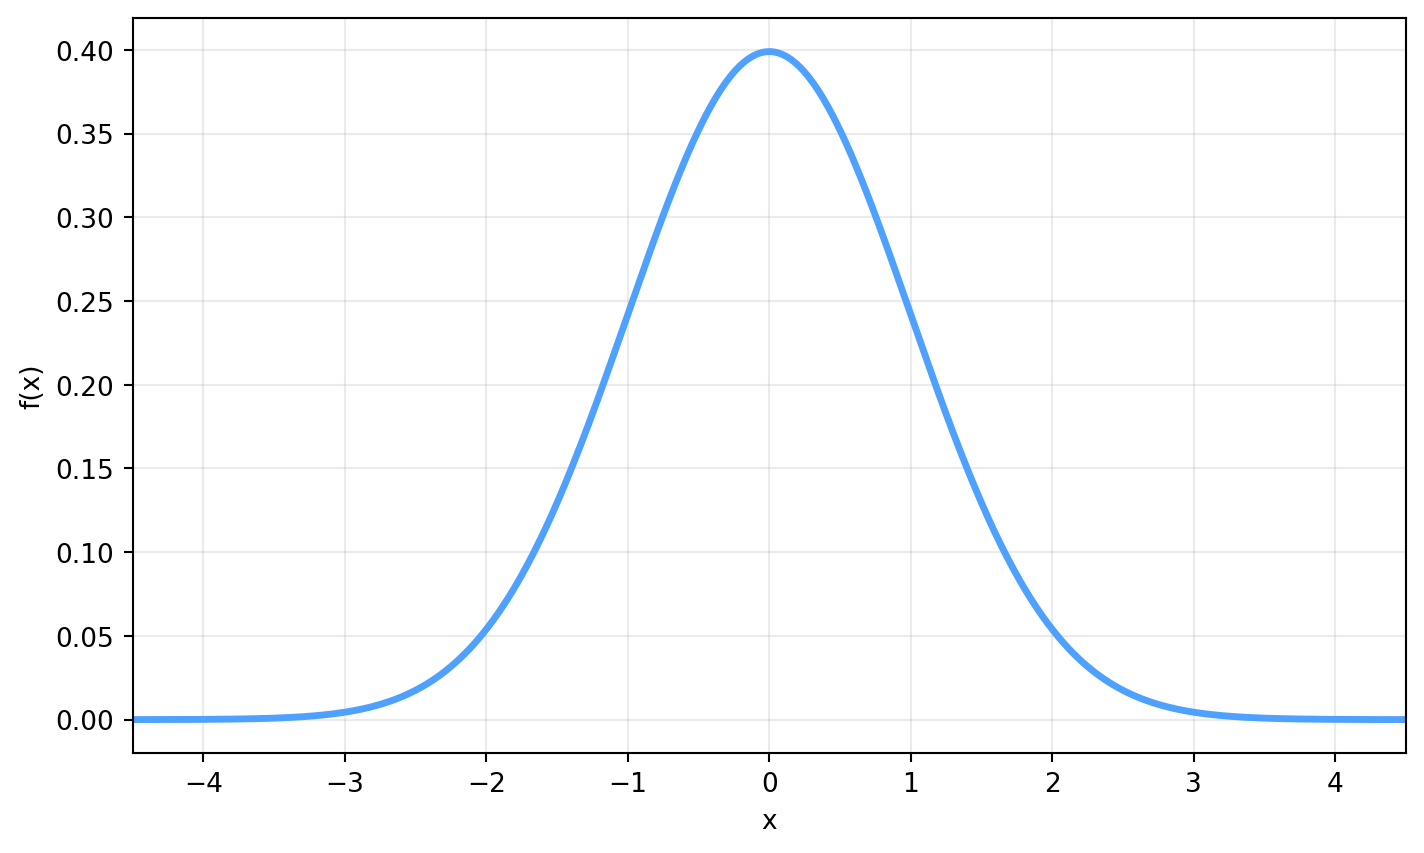
\includegraphics[keepaspectratio]{chapters/../assets/figures/gaussian_standard_density.png}}

}

\caption{\label{fig-standard-normal-density}Плотность стандартного
нормального распределения с математическим ожиданием \(0\) и дисперсией
\(1\)}

\end{figure}%

Площадь под всей кривой равна единице. Высота кривой является
плотностью; вероятность задаётся площадью над выбранным интервалом оси
\(x\).

\subsection{Стандартизация}\label{ux441ux442ux430ux43dux434ux430ux440ux442ux438ux437ux430ux446ux438ux44f}

Если \(X\sim\mathcal N(\mu,\sigma^2)\), то линейное преобразование

\begin{equation}\protect\phantomsection\label{eq-normal-standardization}{
Z=\frac{X-\mu}{\sigma}
}\end{equation}

даёт \(Z\sim\mathcal N(0,1)\). Число \(z\) показывает отклонение от
среднего в единицах стандартного отклонения. Результат \(x=\mu+2\sigma\)
соответствует \(z=2\) при любых \(\mu\) и \(\sigma\).

\section{Квантили стандартного нормального
распределения}\label{ux43aux432ux430ux43dux442ux438ux43bux438-ux441ux442ux430ux43dux434ux430ux440ux442ux43dux43eux433ux43e-ux43dux43eux440ux43cux430ux43bux44cux43dux43eux433ux43e-ux440ux430ux441ux43fux440ux435ux434ux435ux43bux435ux43dux438ux44f}

Кумулятивная функция стандартной нормальной величины равна

\begin{equation}\protect\phantomsection\label{eq-standard-normal-cdf}{
\begin{aligned}
\Phi(z)
&=P(Z\le z)\\
&=\frac{1}{\sqrt{2\pi}}
\int_{-\infty}^{z}e^{-t^2/2}\,dt\\
&=\frac12\left[1+\operatorname{erf}\!\left(\frac{z}{\sqrt2}\right)\right].
\end{aligned}
}\end{equation}

Квантиль уровня \(\beta\) --- это число \(z_\beta\), для которого

\begin{equation}\protect\phantomsection\label{eq-standard-normal-quantile}{
\Phi(z_\beta)=\beta.
}\end{equation}

Иными словами, слева от \(z_\beta\) лежит доля вероятности \(\beta\).
Несколько часто используемых значений собраны в таблице
\ref{tbl-standard-normal-quantiles}.

\begin{longtable}[]{@{}rr@{}}
\caption{Квантили стандартного нормального
распределения}\label{tbl-standard-normal-quantiles}\tabularnewline
\toprule\noalign{}
\(\beta\) & \(z_\beta\) \\
\midrule\noalign{}
\endfirsthead
\toprule\noalign{}
\(\beta\) & \(z_\beta\) \\
\midrule\noalign{}
\endhead
\bottomrule\noalign{}
\endlastfoot
\(0.900\) & \(1.282\) \\
\(0.950\) & \(1.645\) \\
\(0.975\) & \(1.960\) \\
\(0.995\) & \(2.576\) \\
\end{longtable}

Рисунок \ref{fig-standard-normal-quantiles} показывает, как
горизонтальный уровень \(\beta\) на графике CDF определяет квантиль
\(z_\beta\).

\begin{figure}

\centering{

\pandocbounded{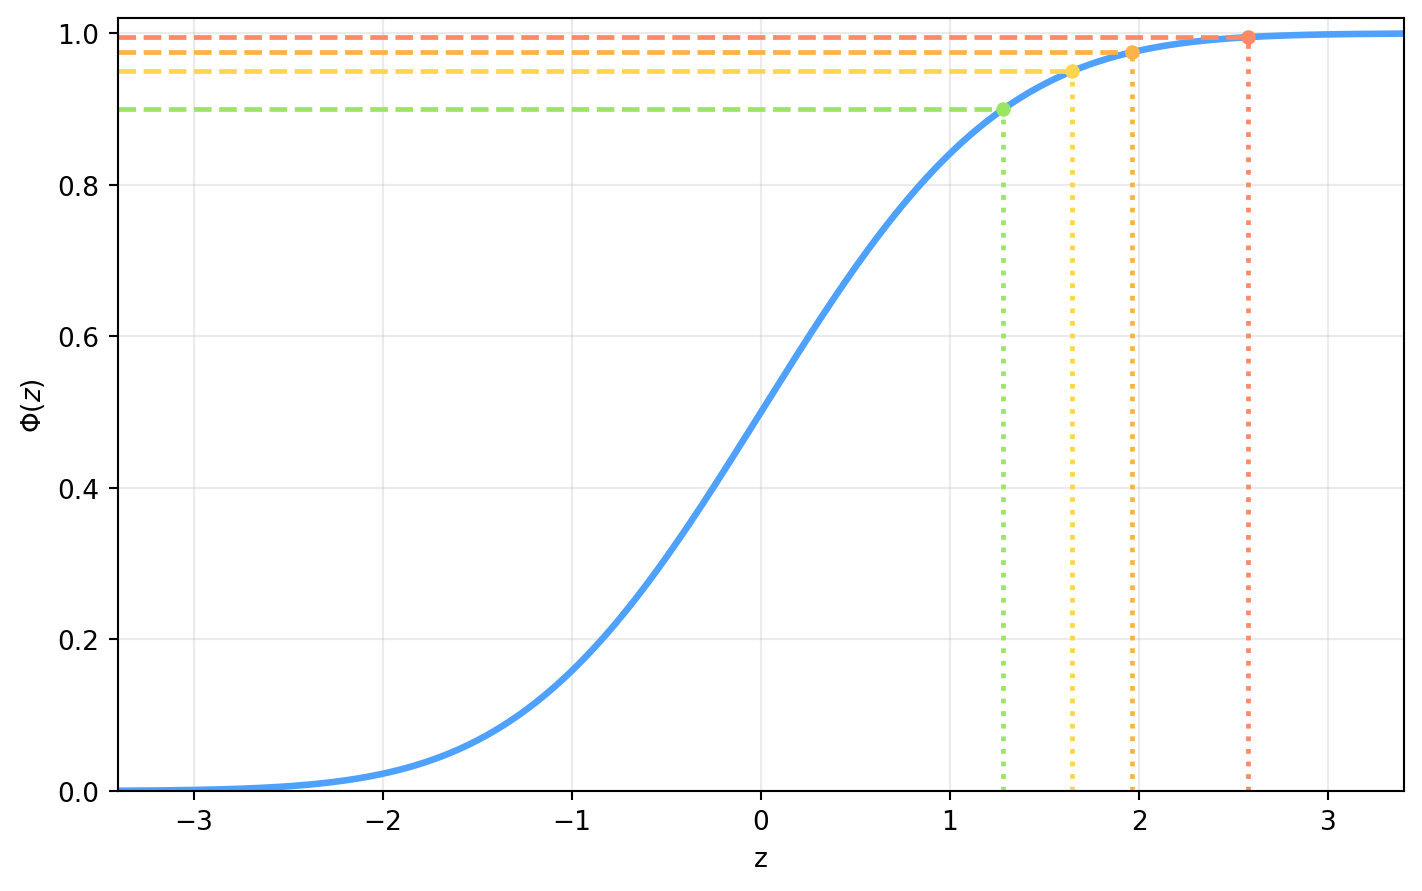
\includegraphics[keepaspectratio]{chapters/../assets/figures/normal_quantile_cdf.png}}

}

\caption{\label{fig-standard-normal-quantiles}Кумулятивная функция
стандартного нормального распределения; пунктирные линии отмечают уровни
\(\beta\) и соответствующие квантили \(z_\beta\)}

\end{figure}%

\section{Центральные интервалы}\label{interactive-central-intervals}

Квантиль \(z_\beta\) из уравнения \ref{eq-standard-normal-quantile}
отсекает один левый хвост. Для симметричного распределения часто
выбирают центральную область и оставляют в обоих хвостах одинаковую
вероятность.

Пусть вероятность центральной области равна \(\gamma\), а полная
вероятность двух хвостов равна \(\alpha=1-\gamma\). Тогда

\begin{equation}\protect\phantomsection\label{eq-gaussian-central-region}{
P(-c\le Z\le c)=\gamma,
\qquad
P(Z<-c)=P(Z>c)=\frac{\alpha}{2},
}\end{equation}

и граница области выражается через квантиль:

\begin{equation}\protect\phantomsection\label{eq-gaussian-central-critical-value}{
c=z_{(1+\gamma)/2}=z_{1-\alpha/2}.
}\end{equation}

Для границ \(c=1\), \(2\) и \(3\) получаются значения из таблицы
\ref{tbl-gaussian-sigma-coverage}.

\begin{longtable}[]{@{}
  >{\centering\arraybackslash}p{(\linewidth - 4\tabcolsep) * \real{0.3846}}
  >{\raggedleft\arraybackslash}p{(\linewidth - 4\tabcolsep) * \real{0.3077}}
  >{\raggedleft\arraybackslash}p{(\linewidth - 4\tabcolsep) * \real{0.3077}}@{}}
\caption{Вероятности центральных гауссовых
областей}\label{tbl-gaussian-sigma-coverage}\tabularnewline
\toprule\noalign{}
\begin{minipage}[b]{\linewidth}\centering
Центральная область
\end{minipage} & \begin{minipage}[b]{\linewidth}\raggedleft
Вероятность внутри \(\gamma\)
\end{minipage} & \begin{minipage}[b]{\linewidth}\raggedleft
Вероятность каждого хвоста
\end{minipage} \\
\midrule\noalign{}
\endfirsthead
\toprule\noalign{}
\begin{minipage}[b]{\linewidth}\centering
Центральная область
\end{minipage} & \begin{minipage}[b]{\linewidth}\raggedleft
Вероятность внутри \(\gamma\)
\end{minipage} & \begin{minipage}[b]{\linewidth}\raggedleft
Вероятность каждого хвоста
\end{minipage} \\
\midrule\noalign{}
\endhead
\bottomrule\noalign{}
\endlastfoot
\(|Z|<1\) & \(0.6827\) & \(0.1587\) \\
\(|Z|<2\) & \(0.9545\) & \(0.0228\) \\
\(|Z|<3\) & \(0.9973\) & \(0.00135\) \\
\end{longtable}

\begin{figure}

\centering{

\pandocbounded{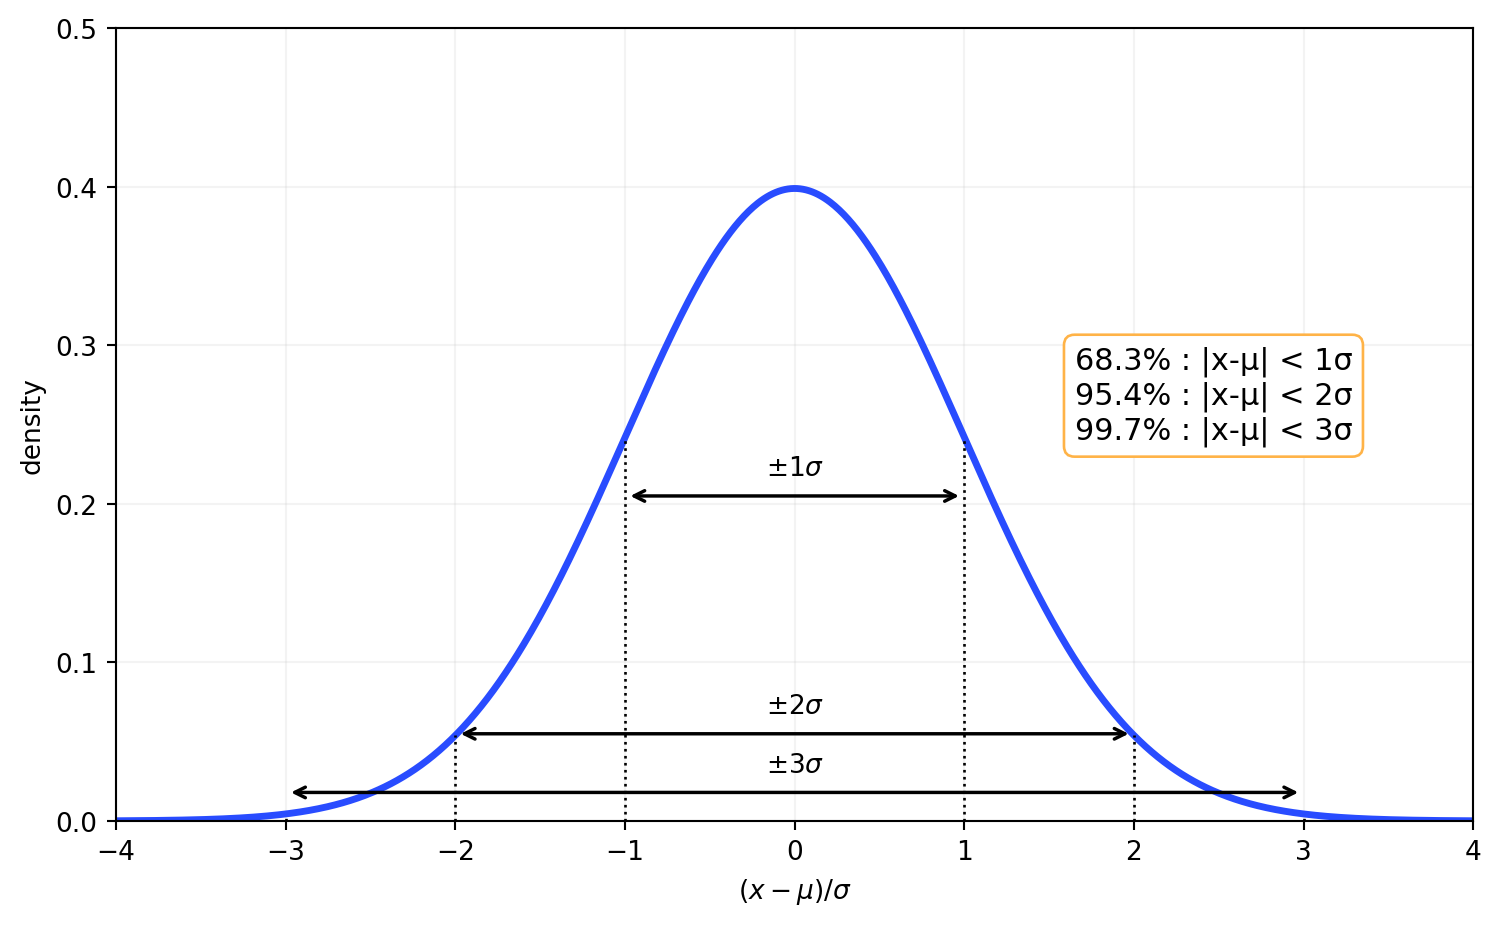
\includegraphics[keepaspectratio]{chapters/../assets/figures/normal_central_intervals.png}}

}

\caption{\label{fig-normal-central-intervals}Плотность стандартного
нормального распределения и центральные области в пределах одного, двух
и трёх стандартных отклонений}

\end{figure}%

На рисунке \ref{fig-normal-central-intervals} границы \(\pm k\sigma\)
отмечены на одной гауссовой кривой. Запись «интервал \(1\sigma\)»
означает одну \(\sigma\) в каждую сторону от среднего; полная ширина
такого интервала равна \(2\sigma\).

В физике частиц порог открытия обычно задают односторонней гауссовой
значимостью \(5\sigma\). Соответствующая хвостовая вероятность равна

\begin{equation}\protect\phantomsection\label{eq-five-sigma-one-sided-tail}{
p_0=P(Z\ge5)=1-\Phi(5)\approx2.87\cdot10^{-7}.
}\end{equation}

Одностороннее и двустороннее соглашения дают разные вероятности при
одном числе сигм. Кроме того, локальная хвостовая вероятность меняется
после учёта поиска во многих точках параметра, а систематические
неопределённости входят в саму статистическую модель. Надпись
\(5\sigma\) не выполняет эти вычисления за исследователя {[}2{]}.

\section{Совместимость двух измерений}\label{interactive-compatibility}

Пусть два измерения одной физической величины дали

\begin{equation}\protect\phantomsection\label{eq-two-measurement-results}{
x_1\pm\sigma_1,
\qquad
x_2\pm\sigma_2.
}\end{equation}

Для начала сравним две пары:

\begin{equation}\protect\phantomsection\label{eq-compatibility-example-wide}{
1.0\pm0.5,
\qquad
2.0\pm0.5,
}\end{equation}

и

\begin{equation}\protect\phantomsection\label{eq-compatibility-example-precise}{
1.010\pm0.001,
\qquad
1.020\pm0.001.
}\end{equation}

В первой паре центральные значения отличаются на единицу, во второй ---
всего на \(0.010\). Этого сравнения недостаточно. Масштаб разности
задают её собственные флуктуации.

\subsection{Распределение
разности}\label{ux440ux430ux441ux43fux440ux435ux434ux435ux43bux435ux43dux438ux435-ux440ux430ux437ux43dux43eux441ux442ux438}

Обозначим результаты ещё не выполненных измерений через \(X_1\) и
\(X_2\) и введём

\begin{equation}\protect\phantomsection\label{eq-measurement-difference}{
D=X_1-X_2.
}\end{equation}

При гипотезе, что оба эксперимента измеряют одно истинное значение
\(\mu\),

\[
\mathbb E[D]=\mu-\mu=0.
\]

Из общей формулы для дисперсии суммы следует

\begin{equation}\protect\phantomsection\label{eq-measurement-difference-variance}{
\operatorname{Var}(D)
=\sigma_1^2+\sigma_2^2
-2\operatorname{cov}(X_1,X_2).
}\end{equation}

Если измерения независимы, ковариация равна нулю и

\begin{equation}\protect\phantomsection\label{eq-independent-difference-uncertainty}{
\sigma_D=\sqrt{\sigma_1^2+\sigma_2^2}.
}\end{equation}

Для независимых гауссовых измерений разность также гауссова. Полученное
значение разности переводится в стандартную нормальную шкалу:

\begin{equation}\protect\phantomsection\label{eq-measurement-compatibility-z}{
z_{\mathrm{obs}}
=\frac{x_1-x_2}{\sqrt{\sigma_1^2+\sigma_2^2}}.
}\end{equation}

Двусторонняя хвостовая вероятность для такой или ещё большей по модулю
разности равна

\begin{equation}\protect\phantomsection\label{eq-measurement-compatibility-pvalue}{
p=2\left[1-\Phi\!\left(|z_{\mathrm{obs}}|\right)\right].
}\end{equation}

Это \(p\)-значение относится к конкретной гипотезе: два измерения имеют
одно среднее, их стандартные отклонения известны, а ошибки независимы и
гауссовы.

\subsection{Центральная область
проверки}\label{ux446ux435ux43dux442ux440ux430ux43bux44cux43dux430ux44f-ux43eux431ux43bux430ux441ux442ux44c-ux43fux440ux43eux432ux435ux440ux43aux438}

Выберем уровень значимости \(\alpha\). Центральная область неотвержения
имеет границу

\begin{equation}\protect\phantomsection\label{eq-compatibility-critical-value}{
c=z_{1-\alpha/2}.
}\end{equation}

Если \(|z_{\mathrm{obs}}|\le c\), гипотеза совместимости не отвергается.
При \(|z_{\mathrm{obs}}|>c\) результат попадает в один из двух хвостов,
и гипотеза отвергается на выбранном уровне \(\alpha\). Та же проверка
записывается короче: \(p\ge\alpha\) или \(p<\alpha\).

Фраза «совместимость не отвергается» выбрана намеренно. Она не
доказывает, что оба измерения правильны. Два эксперимента могут иметь
общий неучтённый сдвиг и прекрасно соглашаться друг с другом.

\begin{semanticpdfbox}[breakable=false]

\begin{center}

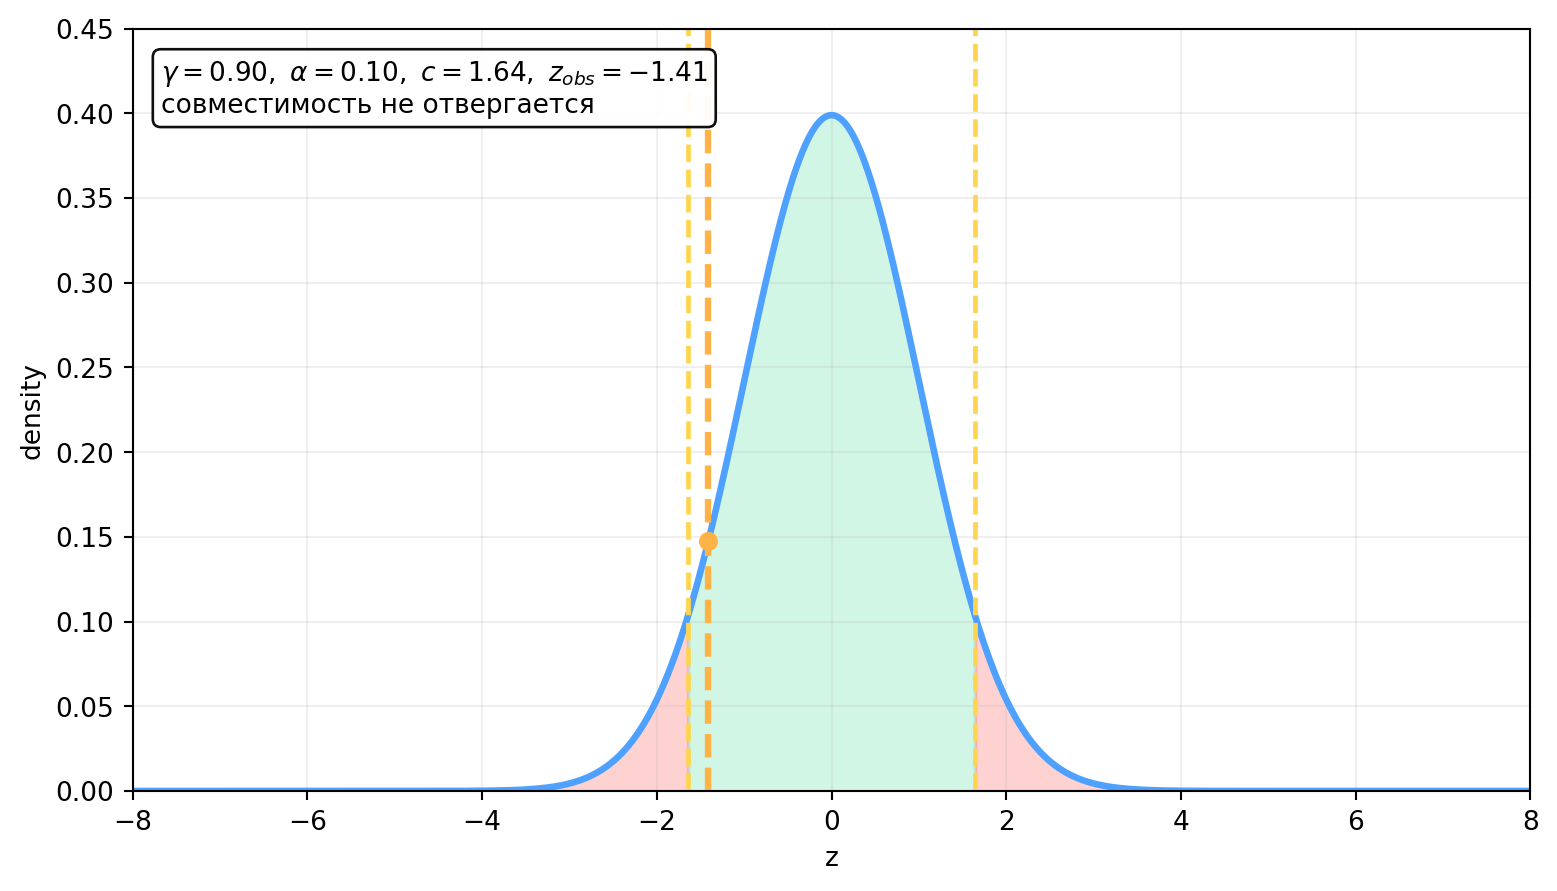
\includegraphics[width=0.74\linewidth,height=\textheight,keepaspectratio,alt={Совместимость двух измерений}]{assets/figures/compatibility_example_a.png}

\end{center}

\noindent\begin{minipage}[c]{\dimexpr\linewidth-30mm\relax}

\textbf{Интерактив}. \textbf{Совместимость двух измерений}

Изменяйте уровень \(\alpha\) и полученное значение \(z_{\mathrm{obs}}\).
На графике показаны центральная область неотвержения, два хвоста и
двустороннее \(p\)-значение.

\end{minipage}\hfill\begin{minipage}[c]{26mm}\centering

\href{https://neutrinohit.github.io/statistical-analysis-course/ru/book/chapters/04_central_limit_theorem.html\#interactive-compatibility}{
\includegraphics[width=24mm,height=\textheight,keepaspectratio,alt={QR-код интерактива}]{assets/qr/compatibility.png}}

\end{minipage}

\end{semanticpdfbox}

\subsection{Два численных
примера}\label{ux434ux432ux430-ux447ux438ux441ux43bux435ux43dux43dux44bux445-ux43fux440ux438ux43cux435ux440ux430}

Для пары из уравнения \ref{eq-compatibility-example-wide}

\begin{equation}\protect\phantomsection\label{eq-compatibility-example-wide-result}{
z_{\mathrm{obs}}
=\frac{1.0-2.0}{\sqrt{0.5^2+0.5^2}}
\approx-1.41,
\qquad
p\approx0.157.
}\end{equation}

При \(\alpha=0.10\) критическая граница равна \(z_{0.95}\approx1.645\).
Полученное значение лежит внутри центральной области, и совместимость не
отвергается.

Для пары из уравнения \ref{eq-compatibility-example-precise}

\begin{equation}\protect\phantomsection\label{eq-compatibility-example-precise-result}{
z_{\mathrm{obs}}
=\frac{1.010-1.020}{\sqrt{0.001^2+0.001^2}}
\approx-7.07,
\qquad
p\approx1.5\cdot10^{-12}.
}\end{equation}

Разность здесь в сто раз меньше, чем в первом примере, и примерно в пять
раз больше в единицах своей неопределённости. Физический смысл имеет
второе сравнение.

\subsection{Общие
неопределённости}\label{ux43eux431ux449ux438ux435-ux43dux435ux43eux43fux440ux435ux434ux435ux43bux451ux43dux43dux43eux441ux442ux438}

Независимость двух измерений часто оказывается приближением.
Эксперименты могут использовать одну внешнюю константу, общий расчёт
потока или одну модель фона. Тогда в уравнении
\ref{eq-measurement-difference-variance} остаётся ковариационный член.

Положительная ковариация уменьшает дисперсию разности: общий сдвиг
сокращается при вычитании. Отрицательная ковариация её увеличивает. Для
совместно гауссовых \(X_1\) и \(X_2\) разность остаётся гауссовой, и
формула \ref{eq-measurement-compatibility-z} обобщается заменой
знаменателя на

\begin{equation}\protect\phantomsection\label{eq-correlated-measurement-compatibility-denominator}{
\sqrt{
\sigma_1^2+\sigma_2^2
-2\operatorname{cov}(X_1,X_2)
}.
}\end{equation}

Если сами неопределённости оценены по небольшим выборкам или
распределения имеют заметные негауссовы хвосты, стандартная нормальная
шкала требует отдельной проверки.

\begin{bookchaptersummary}[Итоги главы]

\begin{itemize}
\tightlist
\item
  Среднее суммы равно сумме средних. В её дисперсию входят дисперсии
  отдельных вкладов и все попарные ковариации.
\item
  Для независимых одинаково распределённых величин с конечной ненулевой
  дисперсией центрированная и нормированная сумма сходится к
  стандартному нормальному распределению. Скорость сходимости зависит от
  исходного закона, особенно при работе с хвостами.
\item
  Стандартизация переводит отклонение в единицы \(\sigma\), а квантили
  задают односторонние и центральные области с выбранной вероятностью.
\item
  Совместимость двух гауссовых измерений определяется распределением их
  разности. Общие источники неопределённости входят в её дисперсию через
  ковариацию.
\end{itemize}

\end{bookchaptersummary}

\section{Задачи}\label{ux437ux430ux434ux430ux447ux438-3}

\begin{semanticpdfbox}[colback=BookCoralSoft,borderline west={1.2mm}{0pt}{BookCoral},breakable=false]

\noindent{\sffamily\bfseries\fontsize{11.2}{13.5}\selectfont Задача 1. Квантили и отклонения в сигмах}\par\nopagebreak[4]\vspace{1.2mm}

Пусть \[
X\sim\mathrm{N}(12.0,0.8^2).
\]

Найдите:

\begin{enumerate}
\def\labelenumi{\arabic{enumi}.}
\tightlist
\item
  центральный интервал \(68\%\);
\item
  центральный интервал \(95\%\);
\item
  односторонний квантиль уровня \(0.95\);
\item
  на сколько сигм отклоняется значение \(x=13.4\) от среднего.
\end{enumerate}

\end{semanticpdfbox}

\begin{semanticpdfbox}[colback=BookCoralSoft,borderline west={1.2mm}{0pt}{BookCoral},breakable=false]

\noindent{\sffamily\bfseries\fontsize{11.2}{13.5}\selectfont Задача 2. Совместимость независимых измерений}\par\nopagebreak[4]\vspace{1.2mm}

Три независимых измерения дали: \[
x_1=125.12\pm0.30,\quad
x_2=124.86\pm0.18,\quad
x_3=125.05\pm0.24.
\]

Для каждой из трёх пар вычислите \(z_{ij}\) и двустороннее
\(p\)-значение. Какие пары совместимы на уровне значимости
\(\alpha=0.05\)? Сравните порядок пар по абсолютной разности
\(|x_i-x_j|\) и по \(|z_{ij}|\).

\end{semanticpdfbox}

\begin{semanticpdfbox}[colback=BookCoralSoft,borderline west={1.2mm}{0pt}{BookCoral},breakable=false]

\noindent{\sffamily\bfseries\fontsize{11.2}{13.5}\selectfont Задача 3. Фотоэлектронная статистика}\par\nopagebreak[4]\vspace{1.2mm}

Заряд одного фотоэлектронного импульса имеет среднее
\(q_0=1.0\,\text{пКл}\) и стандартное отклонение
\(s_q=0.4\,\text{пКл}\). Импульсы независимы.

\begin{enumerate}
\def\labelenumi{\arabic{enumi}.}
\tightlist
\item
  Найдите средний полный заряд, его стандартное отклонение и
  относительную ширину для \(N=25\) и \(N=100\) фотоэлектронов.
\item
  Во сколько раз нужно увеличить \(N\), чтобы относительная ширина
  уменьшилась вдвое?
\item
  Какое распределение полного заряда ожидается при большом фиксированном
  \(N\)? Запишите нормированную величину, к которой применяется ЦПТ.
\end{enumerate}

\end{semanticpdfbox}

\section*{Литература}\label{ux43bux438ux442ux435ux440ux430ux442ux443ux440ux430-3}
\addcontentsline{toc}{section}{Литература}

\markright{Литература}

\protect\phantomsection\label{refs}
\begin{CSLReferences}{0}{0}
\bibitem[\citeproctext]{ref-feller1971}
{[}1{]} Feller, W. \emph{An Introduction to Probability Theory and Its
Applications}. John Wiley \& Sons. 1971.

\bibitem[\citeproctext]{ref-cowan1998}
{[}2{]} Cowan, G. \emph{Statistical Data Analysis}. Oxford University
Press. 1998.

\end{CSLReferences}

\chapter{Когда гаусс не
возникает}\label{ux43aux43eux433ux434ux430-ux433ux430ux443ux441ux441-ux43dux435-ux432ux43eux437ux43dux438ux43aux430ux435ux442}

\bookchapteropeningcontents

\begin{bookchapteropening}[Аннотация]

В прошлой главе мы увидели, как сумма независимых случайных вкладов
приходит к распределению Гаусса. Теперь разберём случаи, в которых этот
вывод применять нельзя или до гауссова предела приходится ждать слишком
долго.

Начнём с распределений Коши и Ландау, у которых нет конечной дисперсии.
Затем посмотрим, как корреляции меняют закон убывания ошибки, чем смесь
распределений отличается от суммы и почему отношение двух гауссовых
величин может иметь длинные хвосты.

\end{bookchapteropening}

\section{Физическая задача: ионизационные потери в трековом
детекторе}\label{ux444ux438ux437ux438ux447ux435ux441ux43aux430ux44f-ux437ux430ux434ux430ux447ux430-ux438ux43eux43dux438ux437ux430ux446ux438ux43eux43dux43dux44bux435-ux43fux43eux442ux435ux440ux438-ux432-ux442ux440ux435ux43aux43eux432ux43eux43c-ux434ux435ux442ux435ux43aux442ux43eux440ux435}

Заряженная частица проходит через трековый детектор и оставляет сигнал в
\(n\) последовательных слоях. По измеренным зарядам

\begin{equation}\protect\phantomsection\label{eq-tracker-charge-samples}{
Q_1,Q_2,\ldots,Q_n
}\end{equation}

нужно оценить её удельные потери энергии \(dE/dx\). Первая идея состоит
в том, чтобы взять среднее:

\begin{equation}\protect\phantomsection\label{eq-tracker-ordinary-mean}{
\overline Q_n=\frac1n\sum_{i=1}^{n}Q_i.
}\end{equation}

Если \(Q_i\) независимы и имеют конечную дисперсию \(\sigma_Q^2\), то

\begin{equation}\protect\phantomsection\label{eq-tracker-mean-variance}{
\operatorname{Var}(\overline Q_n)=\frac{\sigma_Q^2}{n}.
}\end{equation}

Можно ожидать, что с ростом числа слоёв распределение среднего станет
узким и гауссовым. Однако распределение заряда в одном тонком слое имеет
длинный правый хвост. Иногда частица передаёт большую энергию одному
электрону, и один \(Q_i\) оказывается намного больше остальных. Обычное
среднее полностью сохраняет этот вклад.

В газовых трековых детекторах часто используют \textbf{усечённое
среднее}. Заряды сначала располагают по возрастанию,

\begin{equation}\protect\phantomsection\label{eq-tracker-ordered-charges}{
Q_{(1)}\le Q_{(2)}\le\cdots\le Q_{(n)},
}\end{equation}

а затем усредняют только \(m\) меньших значений:

\begin{equation}\protect\phantomsection\label{eq-tracker-truncated-mean}{
\overline Q_{\mathrm{tr}}
=\frac1m\sum_{i=1}^{m}Q_{(i)},
\qquad m<n.
}\end{equation}

Так редкие большие потери не определяют оценку \(dE/dx\). Выбор доли
отбрасываемых измерений зависит от детектора и оптимизируется по его
разрешению. Причину длинного хвоста мы получим ниже из спектра передачи
энергии электрону {[}1{]}.

Этот пример сразу ставит правильный вопрос. Число слагаемых само по себе
ещё не определяет форму суммы. Нужно знать распределение отдельных
вкладов и связи между ними.

\section{Что именно утверждает центральная предельная
теорема}\label{ux447ux442ux43e-ux438ux43cux435ux43dux43dux43e-ux443ux442ux432ux435ux440ux436ux434ux430ux435ux442-ux446ux435ux43dux442ux440ux430ux43bux44cux43dux430ux44f-ux43fux440ux435ux434ux435ux43bux44cux43dux430ux44f-ux442ux435ux43eux440ux435ux43cux430}

Пусть

\begin{equation}\protect\phantomsection\label{eq-ch5-random-sum}{
S_n=X_1+X_2+\cdots+X_n.
}\end{equation}

Для независимых одинаково распределённых величин с параметрами

\begin{equation}\protect\phantomsection\label{eq-ch5-iid-moments}{
\mathbb E[X_i]=\mu,
\qquad
0<\operatorname{Var}(X_i)=\sigma^2<\infty
}\end{equation}

центральная предельная теорема даёт

\begin{equation}\protect\phantomsection\label{eq-ch5-central-limit-theorem}{
Z_n=
\frac{S_n-n\mu}{\sigma\sqrt n}
=\frac{S_n/n-\mu}{\sigma/\sqrt n}
\xrightarrow[n\to\infty]{d}\mathcal N(0,1).
}\end{equation}

В этой формулировке содержатся четыре условия, которые понадобится
проверять.

\begin{itemize}
\tightlist
\item
  Рассматривается сумма случайных величин.
\item
  Слагаемые независимы и имеют одно распределение.
\item
  Их дисперсия конечна.
\item
  Переход к пределу выполняется после центрирования и нормировки суммы.
\end{itemize}

Для независимых величин с разными распределениями существуют более общие
варианты теоремы. Условия Линдеберга и Ляпунова запрещают одному
слагаемому сохранять конечную долю полной дисперсии. Для некоторых
зависимых последовательностей также доказаны свои предельные теоремы
{[}2{]}. Но из одной фразы «слагаемых много» ни одна из них не следует.

Общая формула для дисперсии суммы имеет вид

\begin{equation}\protect\phantomsection\label{eq-ch5-sum-variance}{
\operatorname{Var}(S_n)
=\sum_{i=1}^{n}\operatorname{Var}(X_i)
+2\sum_{i<j}\operatorname{cov}(X_i,X_j).
}\end{equation}

При независимых слагаемых ковариации равны нулю. Корреляции оставляют
вторую сумму и могут полностью изменить зависимость ширины от \(n\).
Если дисперсия \(X_i\) не существует, нормировка через \(\sqrt n\)
лишается основания.

\section{Распределение
Коши}\label{ux440ux430ux441ux43fux440ux435ux434ux435ux43bux435ux43dux438ux435-ux43aux43eux448ux438-1}

Стандартное распределение Коши имеет плотность

\begin{equation}\protect\phantomsection\label{eq-ch5-cauchy-density}{
f_X(x)=\frac{1}{\pi(1+x^2)}.
}\end{equation}

Его кумулятивная функция распределения равна

\begin{equation}\protect\phantomsection\label{eq-ch5-cauchy-cdf}{
F_X(x)=\frac12+\frac1\pi\arctan x.
}\end{equation}

Поэтому величину с распределением Коши можно получить из равномерной
\(U\sim U(0,1)\) преобразованием

\begin{equation}\protect\phantomsection\label{eq-ch5-cauchy-inverse-transform}{
X=F_X^{-1}(U)
=\tan\!\left[\pi\left(U-\frac12\right)\right].
}\end{equation}

Хвост плотности убывает как \(1/x^2\). Из-за этого

\begin{equation}\protect\phantomsection\label{eq-ch5-cauchy-divergent-moments}{
\mathbb E[|X|]=\infty,
\qquad
\mathbb E[X^2]=\infty.
}\end{equation}

Математическое ожидание распределения Коши не существует. Симметричное
главное значение интеграла равно нулю, но математическим ожиданием оно
не является.

\subsection{Среднее Коши не сужается}\label{interactive-cauchy-mean}

Пусть \(X_1,\ldots,X_n\) --- независимые стандартные величины Коши. В
главе 3 мы нашли характеристическую функцию их суммы:

\begin{equation}\protect\phantomsection\label{eq-ch5-cauchy-sum-characteristic}{
\varphi_{S_n}(t)=e^{-n|t|},
\qquad
S_n=\sum_{i=1}^{n}X_i.
}\end{equation}

Это характеристическая функция распределения Коши с масштабом \(n\).
Деление суммы на \(n\) возвращает исходный масштаб:

\begin{equation}\protect\phantomsection\label{eq-ch5-cauchy-average}{
\frac{S_n}{n}\sim\operatorname{Cauchy}(0,1).
}\end{equation}

Распределение среднего при \(n=1\) и \(n=200\) совпадает. Для гауссовых
слагаемых ширина среднего уменьшилась бы в \(\sqrt{200}\) раз.

\begin{semanticpdfbox}[breakable=false]

\begin{center}

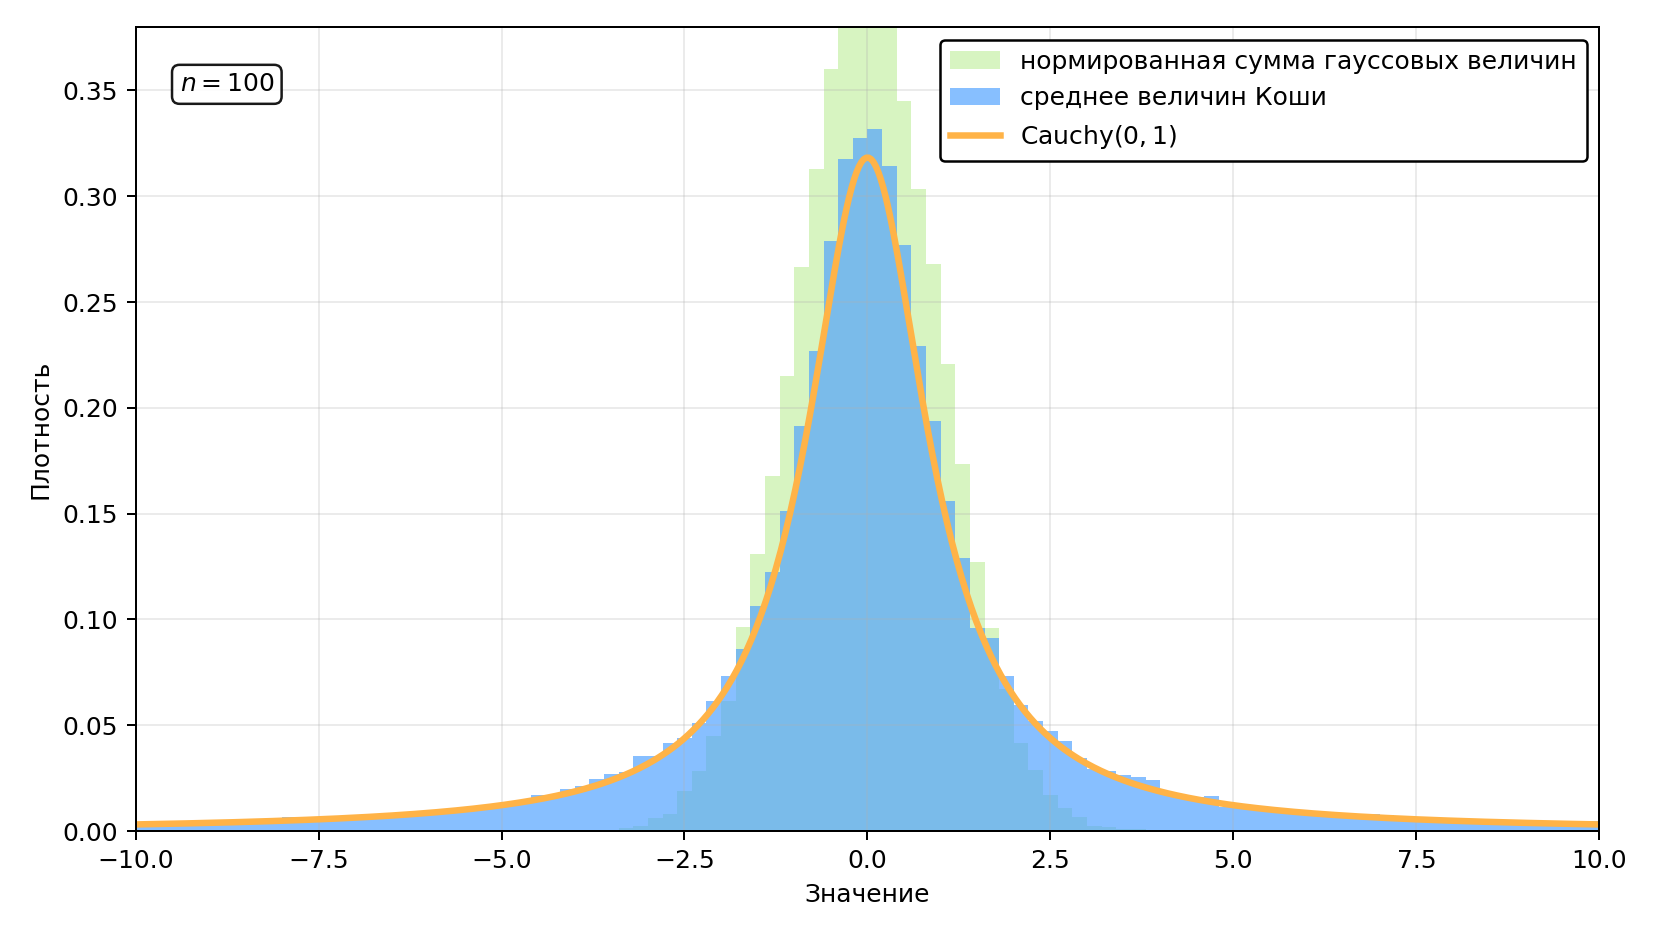
\includegraphics[width=0.74\linewidth,height=\textheight,keepaspectratio,alt={Среднее распределения Коши}]{assets/figures/cauchy_mean_n100.png}

\end{center}

\noindent\begin{minipage}[c]{\dimexpr\linewidth-30mm\relax}

\textbf{Интерактив}. \textbf{Среднее распределения Коши}

Меняя число слагаемых, можно сравнить среднее величин Коши с
нормированной суммой гауссовых величин.

\end{minipage}\hfill\begin{minipage}[c]{26mm}\centering

\href{https://neutrinohit.github.io/statistical-analysis-course/ru/book/chapters/05_non_gaussian_clt_violations.html\#interactive-cauchy-mean}{
\includegraphics[width=24mm,height=\textheight,keepaspectratio,alt={QR-код интерактива}]{assets/qr/cauchy_mean.png}}

\end{minipage}

\end{semanticpdfbox}

Распределение Коши встречается и в физике. Нерелятивистская линия
Брейта---Вигнера имеет ту же форму и служит простой моделью резонансного
пика. Для релятивистского резонанса форма зависит от выбранной
кинематической переменной и фазового пространства.

Из поведения среднего не следует, что накопление данных для
распределения Коши бесполезно. Параметр положения можно оценивать по
медиане или методом максимального правдоподобия. Эти оценки используют
форму распределения и не требуют существования \(\mathbb E[X]\).

\section{Энергетические потери в тонком слое
вещества}\label{ux44dux43dux435ux440ux433ux435ux442ux438ux447ux435ux441ux43aux438ux435-ux43fux43eux442ux435ux440ux438-ux432-ux442ux43eux43dux43aux43eux43c-ux441ux43bux43eux435-ux432ux435ux449ux435ux441ux442ux432ux430}

Вернёмся к задаче, с которой началась глава. Заряженная частица теряет
энергию во множестве актов ионизации и возбуждения. Полную потерю
энергии в слое запишем как

\begin{equation}\protect\phantomsection\label{eq-ch5-energy-loss-sum}{
\Delta=\omega_1+\omega_2+\cdots+\omega_N,
}\end{equation}

где \(\omega_a\) --- энергия, переданная в одном столкновении. Формально
перед нами сумма. Форма распределения определяется хвостом отдельных
\(\omega_a\).

\subsection{Редкие большие передачи
энергии}\label{ux440ux435ux434ux43aux438ux435-ux431ux43eux43bux44cux448ux438ux435-ux43fux435ux440ux435ux434ux430ux447ux438-ux44dux43dux435ux440ux433ux438ux438}

Для быстрой тяжёлой заряженной частицы дифференциальное сечение передачи
энергии электрону в существенной для хвоста области ведёт себя как

\begin{equation}\protect\phantomsection\label{eq-ch5-energy-transfer-spectrum}{
\frac{d\sigma}{d\omega}\propto\frac1{\omega^2},
\qquad
\omega\le W_{\max}.
}\end{equation}

Здесь \(W_{\max}\) --- максимальная передаваемая энергия, заданная
кинематикой столкновения. Вероятность передачи больше порога \(W\)
пропорциональна

\begin{equation}\protect\phantomsection\label{eq-ch5-large-transfer-probability}{
P(\omega>W)
\propto
\int_W^{W_{\max}}\frac{d\omega}{\omega^2}
=\frac1W-\frac1{W_{\max}}.
}\end{equation}

При \(W\ll W_{\max}\) получаем

\begin{equation}\protect\phantomsection\label{eq-ch5-large-transfer-tail}{
P(\omega>W)\propto\frac1W.
}\end{equation}

Хвост убывает медленно. Один \(\delta\)-электрон может унести заметную
часть энергии, доступной в слое, и дать заряд намного больше наиболее
вероятного. Именно эти события образуют правый хвост распределения
\(Q_i\) в трековом детекторе.

\subsection{Распределение Ландау}\label{interactive-landau-tail}

В идеализированном пределе тонкого слоя распределение потери энергии
имеет ландау-подобную форму

\begin{equation}\protect\phantomsection\label{eq-ch5-landau-location-scale}{
p(\Delta)
=\frac1\xi
L\!\left(\frac{\Delta-\Delta_0}{\xi}\right).
}\end{equation}

Параметр \(\Delta_0\) задаёт положение распределения, а \(\xi\) ---
масштаб флуктуаций. При используемом здесь определении стандартной
функции Ландау \(\Delta_0\) не совпадает с наиболее вероятным значением.
Для частицы с зарядом \(ze\) в веществе

\begin{equation}\protect\phantomsection\label{eq-ch5-landau-scale}{
\xi=
\frac K2\frac ZA\frac{z^2}{\beta^2}\rho x.
}\end{equation}

Здесь \(Z\) и \(A\) --- атомный номер и молярная масса вещества,
\(\rho x\) --- массовая толщина слоя, \(\beta=v/c\), а
\(K=4\pi N_A r_e^2m_ec^2\simeq0.307\,
\text{МэВ}\,\text{см}^2\,\text{моль}^{-1}\).

Стандартную функцию Ландау можно определить интегралом

\begin{equation}\protect\phantomsection\label{eq-ch5-landau-integral}{
L(\lambda)=
\frac1\pi\int_0^\infty
\exp[-u\ln u-\lambda u]\sin(\pi u)\,du.
}\end{equation}

При больших положительных \(\lambda\)

\begin{equation}\protect\phantomsection\label{eq-ch5-landau-asymptotic-tail}{
L(\lambda)\sim\frac1{\lambda^2}.
}\end{equation}

Наиболее вероятное значение конечно, а среднее и дисперсия идеального
распределения Ландау не определены. Подробное описание флуктуаций
ионизационных потерь в тонких кремниевых детекторах дано в {[}1{]}.

\begin{semanticpdfbox}[breakable=false]

\begin{center}

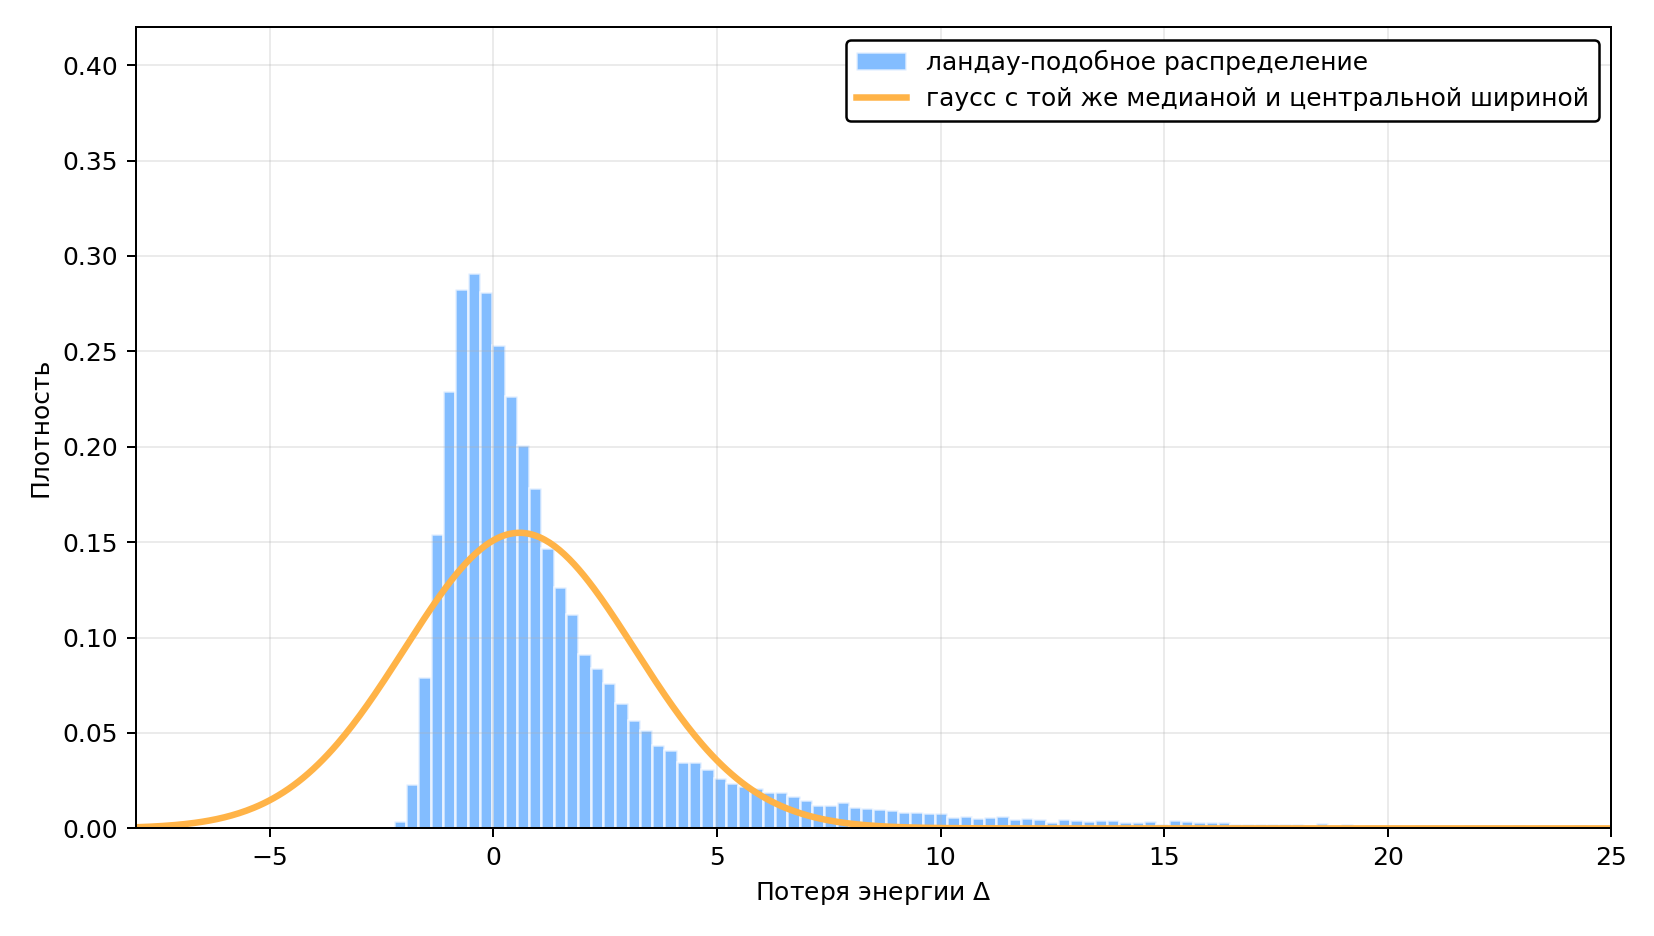
\includegraphics[width=0.74\linewidth,height=\textheight,keepaspectratio,alt={Длинный хвост распределения Ландау}]{assets/figures/landau_like_default.png}

\end{center}

\noindent\begin{minipage}[c]{\dimexpr\linewidth-30mm\relax}

\textbf{Интерактив}. \textbf{Длинный хвост распределения Ландау}

Интерактив сопоставляет ландау-подобное распределение с гауссовой
кривой, имеющей ту же медиану и ту же центральную ширину.

\end{minipage}\hfill\begin{minipage}[c]{26mm}\centering

\href{https://neutrinohit.github.io/statistical-analysis-course/ru/book/chapters/05_non_gaussian_clt_violations.html\#interactive-landau-tail}{
\includegraphics[width=24mm,height=\textheight,keepaspectratio,alt={QR-код интерактива}]{assets/qr/landau_tail.png}}

\end{minipage}

\end{semanticpdfbox}

В идеализированной модели верхнюю границу передачи энергии удаляют.
Тогда хвост \(p(\omega)\propto1/\omega^2\) даёт логарифмически
расходящийся первый момент и линейно расходящийся второй:

\begin{equation}\protect\phantomsection\label{eq-ch5-energy-transfer-divergent-moments}{
\int^\infty \omega\frac{d\omega}{\omega^2}
=\int^\infty\frac{d\omega}{\omega},
\qquad
\int^\infty \omega^2\frac{d\omega}{\omega^2}
=\int^\infty d\omega.
}\end{equation}

Обычная ЦПТ к такой модели неприменима. В реальном столкновении
\(W_{\max}\) конечно. Распределение Ландау, столь любимое
экспериментаторами для описания потерь энергии в тонких детекторах - это
приближение. Если хотите точнее, используйте распределение Вавилова. При
увеличении толщины слоя последнее переходит к гауссову распределению.

Теперь понятна и конструкция из начала главы. Усечённое среднее
подавляет редкие большие \(Q_i\), созданные \(\delta\)-электронами. Цена
этой операции --- потеря части измерений и необходимость отдельно
определить распределение и смещение оценки
\(\overline Q_{\mathrm{tr}}\).

\begin{semanticpdfbox}[colback=BookBiographySoft,borderline west={1.2mm}{0pt}{BookBiography},breakable=false]

\noindent\begin{minipage}[t]{30mm}\vspace{0pt}\centering

\href{https://commons.wikimedia.org/wiki/File:Landau.jpg}{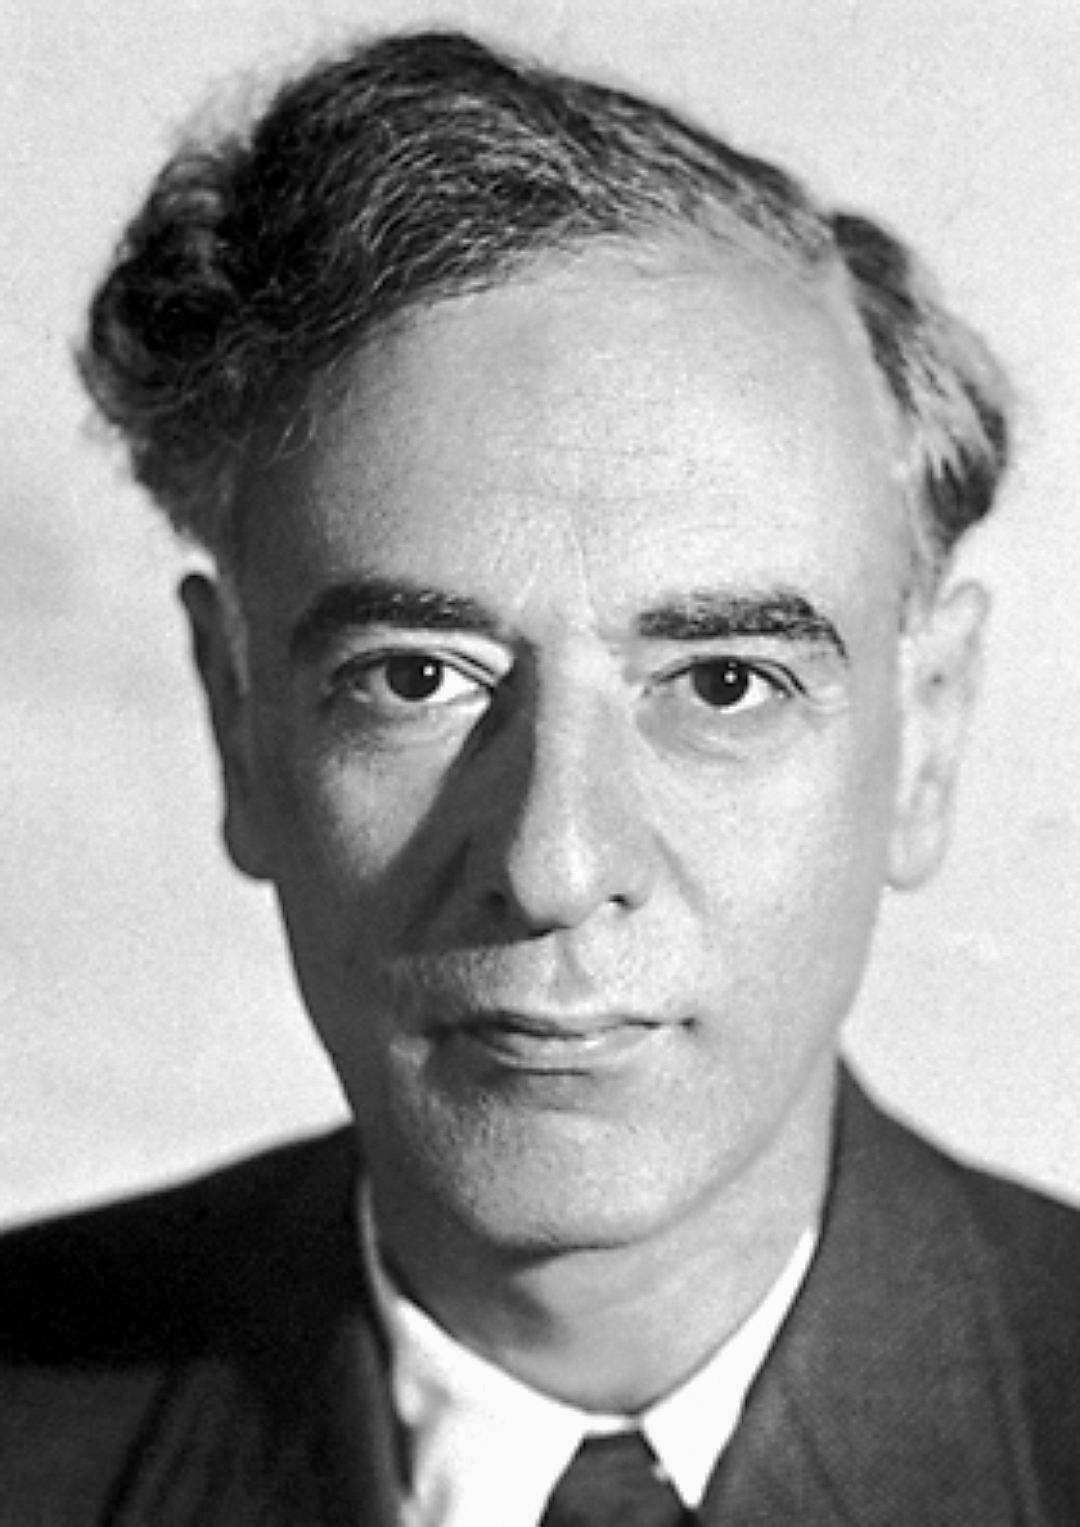
\includegraphics[width=28mm,height=\textheight,keepaspectratio,alt={Портрет Льва Давидовича Ландау}]{assets/people/lev-landau.jpg}}

\end{minipage}\hfill\begin{minipage}[t]{\dimexpr\linewidth-35mm\relax}\vspace{0pt}

{\sffamily\bfseries\footnotesize\color{BookBiography} БИОГРАФИЯ\par}\vspace{0.8mm}{\sffamily\bfseries\large\color{BookInk} Лев Давидович Ландау\par}

{\sffamily\small\color{BookMuted} 1908–1968\par}\vspace{1.4mm}

Лев Ландау - выдающийся советский физик-теоретик. Он разработал
квантовую теорию диамагнетизма, теорию фазовых переходов второго рода,
теорию сверхтекучести жидкого гелия и теорию ферми-жидкости. Вместе с
Виталием Гинзбургом он построил феноменологическую теорию
сверхпроводимости. За работы по теории конденсированного состояния,
прежде всего жидкого гелия, Ландау получил Нобелевскую премию по физике
1962 года.

Для этой главы особенно важна его теория флуктуаций энергетических
потерь быстрой заряженной частицы в тонком слое вещества. Полученное
распределение сохраняет след редких больших передач энергии и имеет
длинный правый хвост.

Лев Ландау и Евгений Лифшиц создали многотомный «Курс теоретической
физики», воспитавший множество поколений учёных в нашей стране и во всём
мире.

{\footnotesize\color{BookMuted}

\textbf{Источник:}
\href{https://www.nobelprize.org/prizes/physics/1962/landau/biographical/}{Nobel Prize};
фото
\href{https://commons.wikimedia.org/wiki/File:Landau.jpg}{архив Нобелевского фонда, общественное достояние}

}

\end{minipage}

\end{semanticpdfbox}

\section{Коррелированные
слагаемые}\label{ux43aux43eux440ux440ux435ux43bux438ux440ux43eux432ux430ux43dux43dux44bux435-ux441ux43bux430ux433ux430ux435ux43cux44bux435}

Ковариационная сумма в уравнении \ref{eq-ch5-sum-variance} исчезает
только для некоррелированных слагаемых. Рассмотрим простой случай:

\begin{equation}\protect\phantomsection\label{eq-ch5-equicorrelated-variables}{
\operatorname{Var}(X_i)=\sigma^2,
\qquad
\operatorname{corr}(X_i,X_j)=\rho,
\quad i\ne j.
}\end{equation}

Для среднего

\begin{equation}\protect\phantomsection\label{eq-ch5-equicorrelated-mean}{
\overline X_n=\frac1n\sum_{i=1}^{n}X_i
}\end{equation}

получаем

\begin{equation}\protect\phantomsection\label{eq-ch5-equicorrelated-mean-variance}{
\begin{aligned}
\operatorname{Var}(\overline X_n)
&=\frac1{n^2}\left[
n\sigma^2+2\frac{n(n-1)}2\rho\sigma^2
\right]\\
&=\frac{\sigma^2}{n}\left[1+(n-1)\rho\right].
\end{aligned}
}\end{equation}

При \(\rho=0\) остаётся \(\sigma^2/n\). При фиксированном \(\rho>0\)

\begin{equation}\protect\phantomsection\label{eq-ch5-equicorrelated-variance-limit}{
\operatorname{Var}(\overline X_n)
\xrightarrow[n\to\infty]{}\rho\sigma^2.
}\end{equation}

Матрица с одинаковой корреляцией всех пар допустима при
\(-1/(n-1)\le\rho\le1\). Поэтому фиксированное отрицательное \(\rho\)
нельзя сохранять при неограниченном росте \(n\). Положительная
корреляция оставляет конечную ширину среднего.

\subsection{Общий сдвиг как систематическая
ошибка}\label{interactive-correlated-errors}

Пусть каждое измерение содержит одну общую и одну независимую
составляющую:

\begin{equation}\protect\phantomsection\label{eq-ch5-common-shift-model}{
X_i=\mu+C+\varepsilon_i.
}\end{equation}

В ансамбле повторных калибровок и измерений зададим

\begin{equation}\protect\phantomsection\label{eq-ch5-common-shift-distributions}{
C\sim\mathcal N(0,\sigma_C^2),
\qquad
\varepsilon_i\sim\mathcal N(0,\sigma_\varepsilon^2),
}\end{equation}

причём \(C\) и все \(\varepsilon_i\) независимы. Тогда

\begin{equation}\protect\phantomsection\label{eq-ch5-common-shift-mean}{
\overline X_n
=\mu+C+\frac1n\sum_{i=1}^{n}\varepsilon_i
}\end{equation}

и

\begin{equation}\protect\phantomsection\label{eq-ch5-common-shift-variance}{
\operatorname{Var}(\overline X_n)
=\sigma_C^2+\frac{\sigma_\varepsilon^2}{n}.
}\end{equation}

Статистический член уменьшается с числом измерений. Общий сдвиг
повторяется во всех \(X_i\) и остаётся целиком. Так ведут себя,
например, неопределённость энергетической шкалы, нормировки потока или
светимости, коэффициента усиления и общий временной сдвиг.

\begin{semanticpdfbox}[breakable=false]

\begin{center}

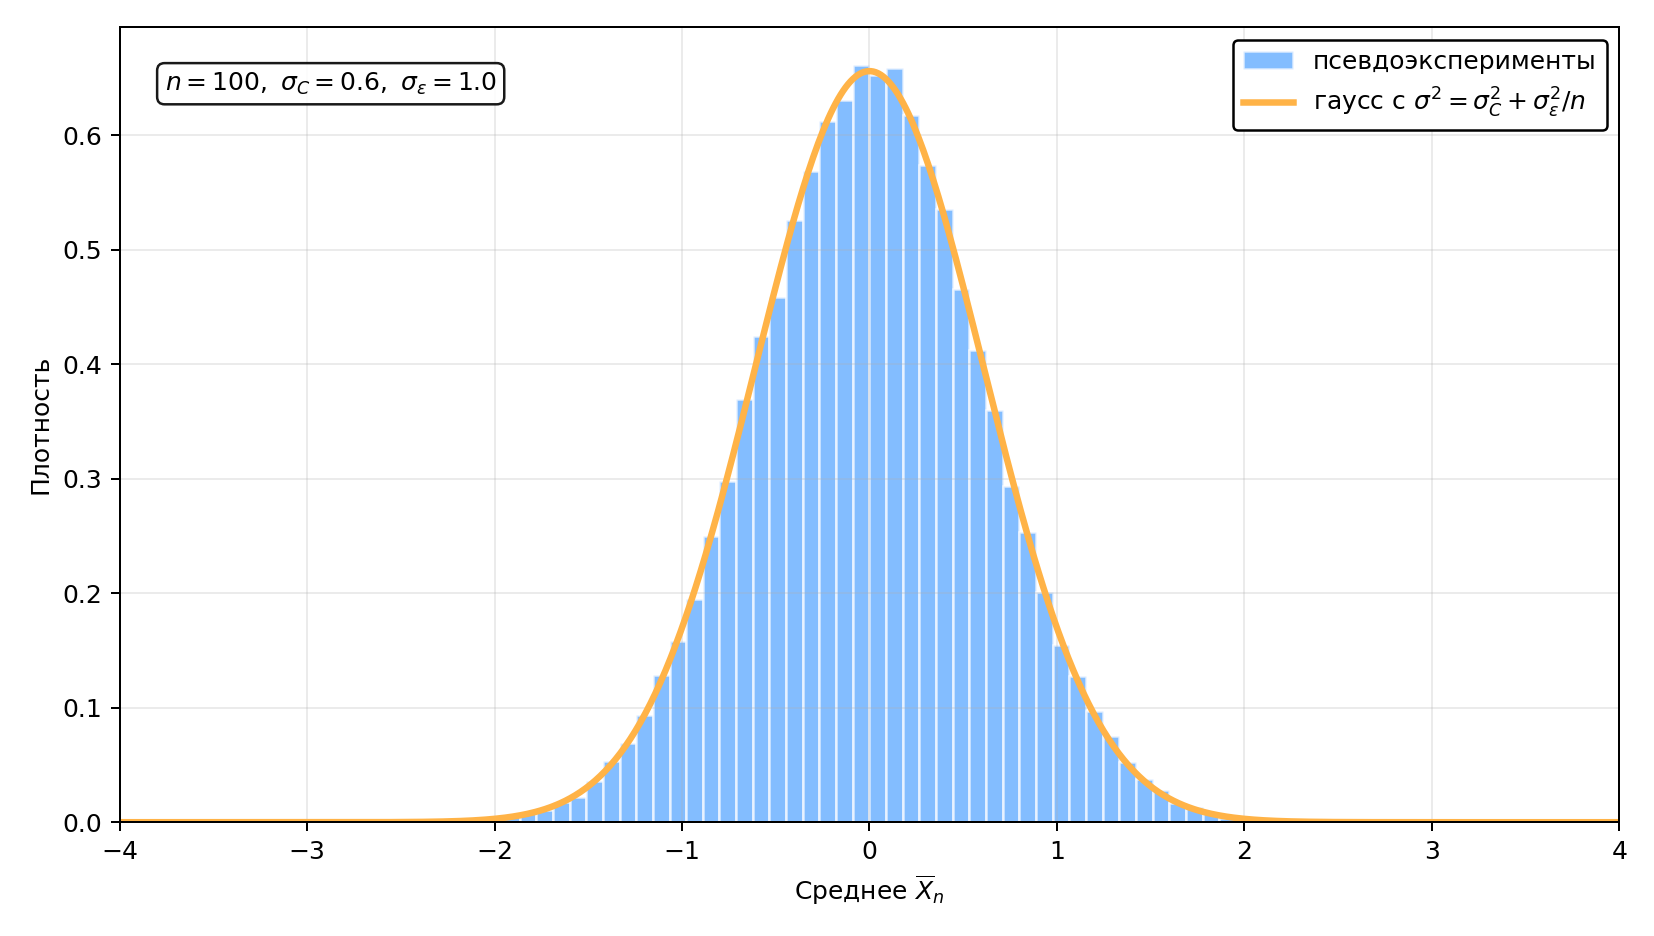
\includegraphics[width=0.74\linewidth,height=\textheight,keepaspectratio,alt={Статистическая и общая ошибки}]{assets/figures/correlated_error_sigma06.png}

\end{center}

\noindent\begin{minipage}[c]{\dimexpr\linewidth-30mm\relax}

\textbf{Интерактив}. \textbf{Статистическая и общая ошибки}

Меняйте статистическую и общую составляющие ошибки и следите за шириной
распределения среднего при росте выборки.

\end{minipage}\hfill\begin{minipage}[c]{26mm}\centering

\href{https://neutrinohit.github.io/statistical-analysis-course/ru/book/chapters/05_non_gaussian_clt_violations.html\#interactive-correlated-errors}{
\includegraphics[width=24mm,height=\textheight,keepaspectratio,alt={QR-код интерактива}]{assets/qr/correlated_errors.png}}

\end{minipage}

\end{semanticpdfbox}

В этой модели \(\overline X_n\) имеет гауссово распределение при любом
\(n\). Однако его ширина стремится к \(\sigma_C\) и не обращается в
нуль. Гауссова форма гистограммы сама по себе не подтверждает закон
\(1/\sqrt n\).

\section{Смеси распределений}\label{interactive-gaussian-mixture}

Сумма и смесь описывают разные устройства эксперимента. Для суммы два
вклада присутствуют в каждом событии. Например, если

\begin{equation}\protect\phantomsection\label{eq-ch5-poisson-components}{
N_1\sim\operatorname{Pois}(1000),
\qquad
N_2\sim\operatorname{Pois}(100)
}\end{equation}

независимы, то

\begin{equation}\protect\phantomsection\label{eq-ch5-poisson-sum}{
N_1+N_2\sim\operatorname{Pois}(1100).
}\end{equation}

В смеси каждое событие принадлежит одному из нескольких классов. Введём
скрытую переменную \(K\in\{1,2\}\) и зададим

\begin{equation}\protect\phantomsection\label{eq-ch5-poisson-mixture-components}{
N\mid K=1\sim\operatorname{Pois}(1000),
\qquad
N\mid K=2\sim\operatorname{Pois}(100).
}\end{equation}

Если класс события не зарегистрирован, в данных остаётся только \(N\).
Даже узкие распределения внутри классов образуют широкую или
многопиковую смесь.

\subsection{Среднее и дисперсия
смеси}\label{ux441ux440ux435ux434ux43dux435ux435-ux438-ux434ux438ux441ux43fux435ux440ux441ux438ux44f-ux441ux43cux435ux441ux438}

Пусть \(X\) при фиксированном классе \(K\) имеет среднее \(\mu_K\) и
дисперсию \(\sigma_K^2\). Полное среднее равно

\begin{equation}\protect\phantomsection\label{eq-ch5-mixture-mean}{
\mathbb E[X]=\mathbb E_K[\mu_K].
}\end{equation}

Формула полной дисперсии разделяет два источника разброса:

\begin{equation}\protect\phantomsection\label{eq-ch5-total-variance}{
\operatorname{Var}(X)
=\mathbb E_K\!\left[\sigma_K^2\right]
+\operatorname{Var}_K(\mu_K).
}\end{equation}

Первое слагаемое усредняет дисперсии внутри классов. Второе измеряет
разброс между их средними.

Для двух равновероятных пуассоновских классов из уравнения
\ref{eq-ch5-poisson-mixture-components}

\begin{equation}\protect\phantomsection\label{eq-ch5-poisson-mixture-mean}{
\mathbb E[N]=\frac{1000+100}{2}=550.
}\end{equation}

Средняя дисперсия внутри классов равна

\begin{equation}\protect\phantomsection\label{eq-ch5-poisson-within-class-variance}{
\mathbb E_K[\operatorname{Var}(N\mid K)]
=\frac{1000+100}{2}=550,
}\end{equation}

а дисперсия условных средних составляет

\begin{equation}\protect\phantomsection\label{eq-ch5-poisson-between-class-variance}{
\operatorname{Var}_K(\mathbb E[N\mid K])
=\frac{(1000-550)^2+(100-550)^2}{2}
=202\,500.
}\end{equation}

Полная дисперсия

\begin{equation}\protect\phantomsection\label{eq-ch5-poisson-mixture-variance}{
\operatorname{Var}(N)=550+202\,500=203\,050
}\end{equation}

почти целиком определяется различием двух классов. Пуассоновские
флуктуации внутри классов дают меньше трёх десятых процента результата.

\begin{semanticpdfbox}[breakable=false]

\begin{center}

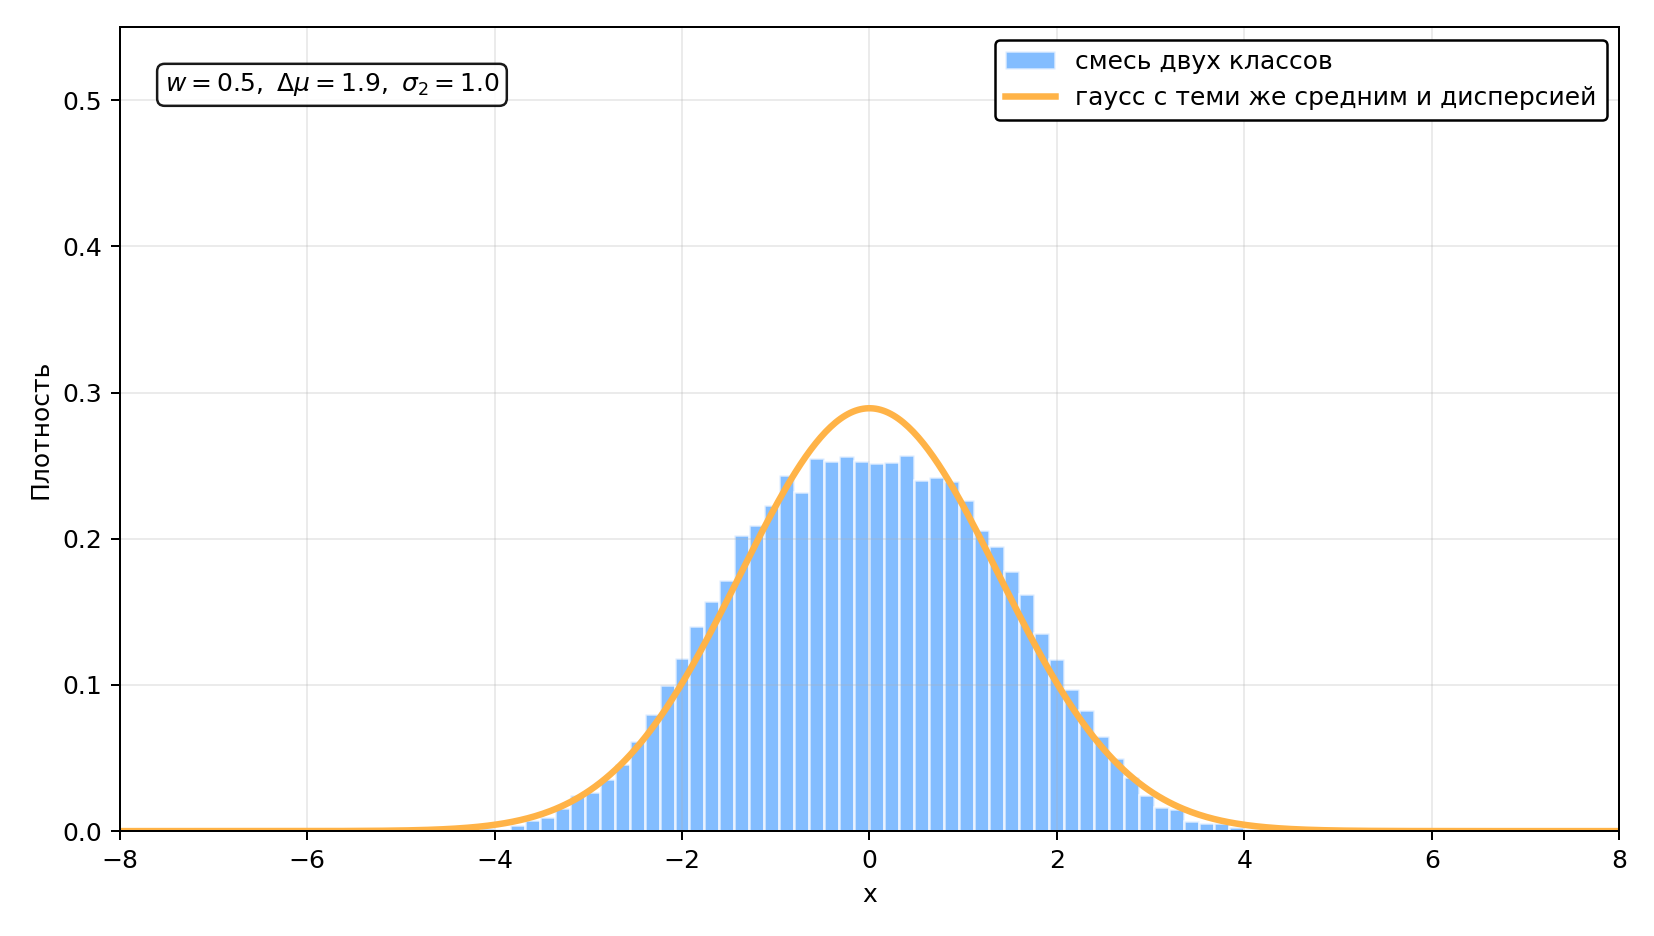
\includegraphics[width=0.74\linewidth,height=\textheight,keepaspectratio,alt={Смесь двух гауссовых классов}]{assets/figures/gaussian_mixture_sep1_9.png}

\end{center}

\noindent\begin{minipage}[c]{\dimexpr\linewidth-30mm\relax}

\textbf{Интерактив}. \textbf{Смесь двух гауссовых классов}

Интерактив показывает, как веса, ширины и расстояние между средними
меняют форму смеси.

\end{minipage}\hfill\begin{minipage}[c]{26mm}\centering

\href{https://neutrinohit.github.io/statistical-analysis-course/ru/book/chapters/05_non_gaussian_clt_violations.html\#interactive-gaussian-mixture}{
\includegraphics[width=24mm,height=\textheight,keepaspectratio,alt={QR-код интерактива}]{assets/qr/gaussian_mixture.png}}

\end{minipage}

\end{semanticpdfbox}

\subsection{Пример: жидкий
сцинтиллятор}\label{ux43fux440ux438ux43cux435ux440-ux436ux438ux434ux43aux438ux439-ux441ux446ux438ux43dux442ux438ux43bux43bux44fux442ux43eux440}

Сигнал жидкосцинтилляционного детектора можно схематично записать как

\begin{equation}\protect\phantomsection\label{eq-ch5-scintillator-signal-model}{
Q=Q(E,K)+Q_{\mathrm{stat}}+Q_{\mathrm{el}},
}\end{equation}

где \(Q_{\mathrm{stat}}\) описывает фотонную статистику,
\(Q_{\mathrm{el}}\) --- шум электроники, а класс \(K\) включает тип
частицы, топологию события, положение в детекторе, долю черенковского
света и другие детали отклика.

Для \(\gamma\)-кванта энергия передаётся нескольким вторичным
электронам:

\begin{equation}\protect\phantomsection\label{eq-ch5-gamma-secondary-electrons}{
\gamma\longrightarrow e_1+e_2+\cdots+e_m,
\qquad
E_\gamma=\sum_{a=1}^{m}E_a.
}\end{equation}

Если световой выход электрона \(L(E)\) нелинеен, средний заряд имеет вид

\begin{equation}\protect\phantomsection\label{eq-ch5-gamma-light-yield}{
Q_\gamma\simeq\sum_{a=1}^{m}L(E_a).
}\end{equation}

При одном и том же \(E_\gamma\) разные наборы \(E_a\) дают разные
значения \(Q_\gamma\). Разброс топологий добавляет к фотонной статистике
второй член из формулы полной дисперсии \ref{eq-ch5-total-variance}.
Описание сигнала одним пуассоновским или гауссовым распределением этот
вклад потеряет.

\section{Отношение случайных величин}\label{interactive-ratio-cauchy}

Центральная предельная теорема относится к суммам. Нелинейное
преобразование может изменить распределение даже при точно гауссовых
исходных величинах.

Пусть \(X\) и \(Y\) независимы и

\begin{equation}\protect\phantomsection\label{eq-ch5-standard-normal-ratio-inputs}{
X,Y\sim\mathcal N(0,1).
}\end{equation}

Для отношения \(R=X/Y\) совместная плотность после замены \(x=ry\) даёт

\begin{equation}\protect\phantomsection\label{eq-ch5-normal-ratio-cauchy}{
\begin{aligned}
f_R(r)
&=\int_{-\infty}^{+\infty}|y|f_X(ry)f_Y(y)\,dy\\
&=\frac1{2\pi}\int_{-\infty}^{+\infty}
|y|\exp\!\left[-\frac{(1+r^2)y^2}{2}\right]dy\\
&=\frac1{\pi(1+r^2)}.
\end{aligned}
}\end{equation}

Получилось стандартное распределение Коши. Отношения появляются при
нормировке сигнала на контрольную область, введении поправки на
эффективность, сравнении двух скоростей счёта и построении асимметрии

\begin{equation}\protect\phantomsection\label{eq-ch5-counting-asymmetry}{
A=\frac{N_1-N_2}{N_1+N_2}.
}\end{equation}

Линейное распространение ошибок для отношения применимо, когда
знаменатель с высокой вероятностью далёк от нуля и его относительная
неопределённость мала. Если знаменатель может оказаться около нуля,
редкие значения отношения уходят далеко в хвост. Симметричная запись
\(r\pm\sigma_r\) перестаёт описывать такое распределение.

\begin{semanticpdfbox}[breakable=false]

\begin{center}

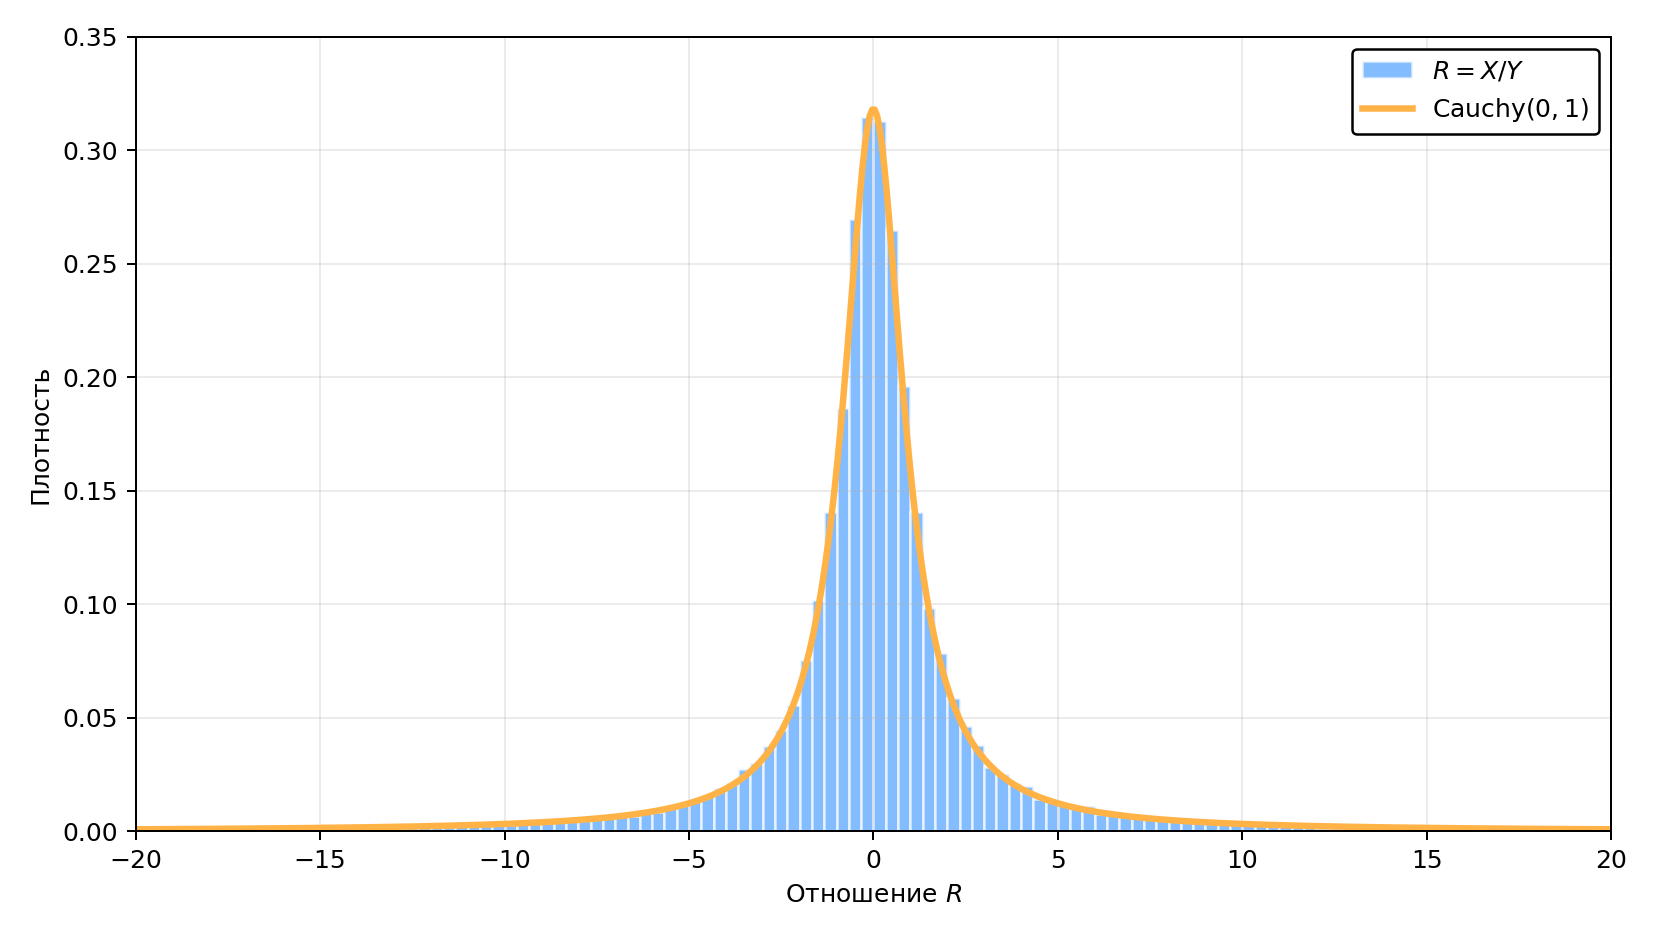
\includegraphics[width=0.74\linewidth,height=\textheight,keepaspectratio,alt={Отношение гауссовых величин}]{assets/figures/ratio_gaussians_cauchy.png}

\end{center}

\noindent\begin{minipage}[c]{\dimexpr\linewidth-30mm\relax}

\textbf{Интерактив}. \textbf{Отношение гауссовых величин}

Меняйте среднее и ширину знаменателя и следите за появлением длинных
хвостов у отношения.

\end{minipage}\hfill\begin{minipage}[c]{26mm}\centering

\href{https://neutrinohit.github.io/statistical-analysis-course/ru/book/chapters/05_non_gaussian_clt_violations.html\#interactive-ratio-cauchy}{
\includegraphics[width=24mm,height=\textheight,keepaspectratio,alt={QR-код интерактива}]{assets/qr/ratio_cauchy.png}}

\end{minipage}

\end{semanticpdfbox}

\section{Причины отклонения от гауссова
приближения}\label{ux43fux440ux438ux447ux438ux43dux44b-ux43eux442ux43aux43bux43eux43dux435ux43dux438ux44f-ux43eux442-ux433ux430ux443ux441ux441ux43eux432ux430-ux43fux440ux438ux431ux43bux438ux436ux435ux43dux438ux44f}

В таблице \ref{tbl-ch5-nongaussian-mechanisms} собраны рассмотренные
причины.

\begin{longtable}[]{@{}
  >{\raggedright\arraybackslash}p{(\linewidth - 4\tabcolsep) * \real{0.3333}}
  >{\raggedright\arraybackslash}p{(\linewidth - 4\tabcolsep) * \real{0.3333}}
  >{\raggedright\arraybackslash}p{(\linewidth - 4\tabcolsep) * \real{0.3333}}@{}}
\caption{Причины отклонения от простого гауссова
приближения}\label{tbl-ch5-nongaussian-mechanisms}\tabularnewline
\toprule\noalign{}
\begin{minipage}[b]{\linewidth}\raggedright
Механизм
\end{minipage} & \begin{minipage}[b]{\linewidth}\raggedright
Какое условие требует проверки
\end{minipage} & \begin{minipage}[b]{\linewidth}\raggedright
Что видно в данных
\end{minipage} \\
\midrule\noalign{}
\endfirsthead
\toprule\noalign{}
\begin{minipage}[b]{\linewidth}\raggedright
Механизм
\end{minipage} & \begin{minipage}[b]{\linewidth}\raggedright
Какое условие требует проверки
\end{minipage} & \begin{minipage}[b]{\linewidth}\raggedright
Что видно в данных
\end{minipage} \\
\midrule\noalign{}
\endhead
\bottomrule\noalign{}
\endlastfoot
Бесконечная дисперсия & Существует ли \(\operatorname{Var}(X_i)\) &
Среднее может не сужаться \\
Тяжёлый хвост & Насколько быстро наступает предельный режим & Редкие
большие значения сохраняются при конечном \(n\) \\
Доминирующий вклад & Мал ли каждый вклад по сравнению со всей суммой &
Форму хвоста задаёт один механизм \\
Корреляции & Независимы ли слагаемые & Ширина не обязана убывать как
\(1/\sqrt n\) \\
Смесь классов & Однородна ли выборка & Возникают дополнительная ширина,
асимметрия или несколько пиков \\
Нелинейное преобразование & Является ли величина суммой & Отношение или
асимметрия наследует границы и хвосты знаменателя \\
\end{longtable}

Проверять гауссово приближение следует на той случайной величине,
которая действительно входит в анализ. Для этого строят
псевдоэксперименты из полной модели и сравнивают распределения при
нескольких размерах выборки. Центральная часть гистограммы может
выглядеть гауссовой раньше хвостов, а именно хвосты определяют
вероятности редких отклонений.

\begin{bookchaptersummary}[Итоги главы]

\begin{itemize}
\tightlist
\item
  Конечная дисперсия и отсутствие доминирующего слагаемого входят в
  условия гауссова предела. У среднего величин Коши ширина не
  уменьшается с ростом выборки.
\item
  Длинный правый хвост ионизационных потерь создают редкие
  \(\delta\)-электроны. В тонком слое используется ландау-подобное
  описание; кинематическая граница передачи энергии приводит к более
  точному распределению Вавилова.
\item
  Положительные корреляции оставляют конечный вклад в дисперсию
  среднего. Общая систематическая ошибка может сохранить гауссову форму
  и одновременно нарушить закон \(1/\sqrt n\).
\item
  Смесь классов получает дополнительную дисперсию от различия условных
  средних. Этот вклад описывается формулой полной дисперсии.
\item
  Отношение двух независимых стандартных гауссовых величин имеет
  распределение Коши. Для нелинейной величины распределение нужно
  выводить отдельно.
\end{itemize}

\end{bookchaptersummary}

\section{Задачи}\label{ux437ux430ux434ux430ux447ux438-4}

\begin{semanticpdfbox}[colback=BookCoralSoft,borderline west={1.2mm}{0pt}{BookCoral},breakable=false]

\noindent{\sffamily\bfseries\fontsize{11.2}{13.5}\selectfont Задача 1. Среднее распределения Коши}\par\nopagebreak[4]\vspace{1.2mm}

Для независимых \(X_i\sim\mathrm{Cauchy}(0,1)\) покажите, что дисперсия
не существует, а \[
\overline X_n=\frac{1}{n}\sum_iX_i
\] имеет то же распределение Коши. Почему это не противоречит ЦПТ?

\end{semanticpdfbox}

\begin{semanticpdfbox}[colback=BookCoralSoft,borderline west={1.2mm}{0pt}{BookCoral},breakable=false]

\noindent{\sffamily\bfseries\fontsize{11.2}{13.5}\selectfont Задача 2. Тяжёлый хвост с конечной дисперсией}\par\nopagebreak[4]\vspace{1.2mm}

Пусть \[
p(x)\sim\frac{C}{|x|^{1+\alpha}}.
\]

\begin{enumerate}
\def\labelenumi{\arabic{enumi}.}
\tightlist
\item
  При каких \(\alpha\) существуют среднее и дисперсия?
\item
  Почему при \(\alpha\) немного больше 2 сходимость к гауссу может быть
  медленной?
\end{enumerate}

\end{semanticpdfbox}

\begin{semanticpdfbox}[colback=BookCoralSoft,borderline west={1.2mm}{0pt}{BookCoral},breakable=false]

\noindent{\sffamily\bfseries\fontsize{11.2}{13.5}\selectfont Задача 3. Один доминирующий вклад}\par\nopagebreak[4]\vspace{1.2mm}

Пусть \[
S=X_0+\epsilon_1+\dots+\epsilon_n,
\] где \(\epsilon_i\sim\mathrm{N}(0,\sigma^2)\), а \(X_0\) негауссов и
\[
\mathrm{Var}(X_0)\gg n\sigma^2.
\] Объясните форму распределения \(S\).

\end{semanticpdfbox}

\begin{semanticpdfbox}[colback=BookCoralSoft,borderline west={1.2mm}{0pt}{BookCoral},breakable=false]

\noindent{\sffamily\bfseries\fontsize{11.2}{13.5}\selectfont Задача 4. Общая систематическая ошибка}\par\nopagebreak[4]\vspace{1.2mm}

Пусть \[
X_i=\mu+C+\epsilon_i,
\] где \(C\sim\mathrm{N}(0,\sigma_C^2)\) и
\(\epsilon_i\sim\mathrm{N}(0,\sigma_\epsilon^2)\). Найдите
\(\mathbb{E}[\overline X_n]\), \(\mathrm{Var}(\overline X_n)\) и предел
дисперсии при \(n\to\infty\).

\end{semanticpdfbox}

\begin{semanticpdfbox}[colback=BookCoralSoft,borderline west={1.2mm}{0pt}{BookCoral},breakable=false]

\noindent{\sffamily\bfseries\fontsize{11.2}{13.5}\selectfont Задача 5. Усреднение коррелированных измерений}\par\nopagebreak[4]\vspace{1.2mm}

Пусть \(n\) величин имеют одинаковую дисперсию \(\sigma^2\) и одинаковый
коэффициент корреляции \(\rho\) для любой пары.

\begin{enumerate}
\def\labelenumi{\arabic{enumi}.}
\tightlist
\item
  Получите дисперсию их среднего.
\item
  Укажите допустимый диапазон \(\rho\) при фиксированном \(n\).
\item
  Рассмотрите случаи \(\rho=0\) и \(\rho>0\) при увеличении \(n\).
\end{enumerate}

\end{semanticpdfbox}

\begin{semanticpdfbox}[colback=BookCoralSoft,borderline west={1.2mm}{0pt}{BookCoral},breakable=false]

\noindent{\sffamily\bfseries\fontsize{11.2}{13.5}\selectfont Задача 6. Смесь двух гауссов}\par\nopagebreak[4]\vspace{1.2mm}

Пусть \[
X|A\sim\mathrm{N}(\mu_A,\sigma_A^2),\qquad
X|B\sim\mathrm{N}(\mu_B,\sigma_B^2),
\] а вероятность класса \(A\) равна \(w\). Найдите полные среднее и
дисперсию. Когда смесь плохо похожа на один гаусс?

\end{semanticpdfbox}

\begin{semanticpdfbox}[colback=BookCoralSoft,borderline west={1.2mm}{0pt}{BookCoral},breakable=false]

\noindent{\sffamily\bfseries\fontsize{11.2}{13.5}\selectfont Задача 7. Скрытая топология в жидком сцинтилляторе}\par\nopagebreak[4]\vspace{1.2mm}

Моноэнергетический \(\gamma\)-квант с энергией \[
E_\gamma=1\ \text{МэВ}
\] может передать энергию вторичным электронам двумя способами: \[
\theta=A:\quad T_1=1\ \text{МэВ},
\] \[
\theta=B:\quad T_1=T_2=0.5\ \text{МэВ}.
\]

Из-за нелинейности светового выхода средние сигналы различаются: \[
Q|\theta=A\sim\mathrm{Pois}(1000),
\qquad
Q|\theta=B\sim\mathrm{Pois}(980).
\] Считайте классы равновероятными.

\begin{enumerate}
\def\labelenumi{\arabic{enumi}.}
\tightlist
\item
  Найдите полное среднее \(\mathbb E[Q]\).
\item
  Вычислите среднюю внутриклассовую дисперсию \[
  \mathbb E_\theta[\mathrm{Var}(Q|\theta)].
  \]
\item
  Вычислите топологический вклад \[
  \mathrm{Var}_\theta(\mathbb E[Q|\theta]).
  \]
\item
  Найдите полную дисперсию и стандартное отклонение \(Q\).
\item
  Сравните результат с пуассоновской моделью \[
  Q\sim\mathrm{Pois}(\mathbb E[Q]).
  \] Какой вклад не описывается этой моделью?
\end{enumerate}

\end{semanticpdfbox}

\begin{semanticpdfbox}[colback=BookCoralSoft,borderline west={1.2mm}{0pt}{BookCoral},breakable=false]

\noindent{\sffamily\bfseries\fontsize{11.2}{13.5}\selectfont Задача 8. Отношение гауссовых величин}\par\nopagebreak[4]\vspace{1.2mm}

Для независимых \(X,Y\sim\mathrm{N}(0,1)\) выведите плотность отношения
\(R=X/Y\) и покажите, что это распределение Коши.

\end{semanticpdfbox}

\section*{Литература}\label{ux43bux438ux442ux435ux440ux430ux442ux443ux440ux430-4}
\addcontentsline{toc}{section}{Литература}

\markright{Литература}

\protect\phantomsection\label{refs}
\begin{CSLReferences}{0}{0}
\bibitem[\citeproctext]{ref-bichsel1988}
{[}1{]} Bichsel, H. Straggling in Thin Silicon Detectors. \emph{Reviews
of Modern Physics}, \textbf{60}, 663--699. 1988.
doi:\href{https://doi.org/10.1103/RevModPhys.60.663}{10.1103/RevModPhys.60.663}.

\bibitem[\citeproctext]{ref-feller1971}
{[}2{]} Feller, W. \emph{An Introduction to Probability Theory and Its
Applications}. John Wiley \& Sons. 1971.

\end{CSLReferences}

\part{II. Моделирование и оценивание}

\chapter{Распространение
ошибок}\label{ux440ux430ux441ux43fux440ux43eux441ux442ux440ux430ux43dux435ux43dux438ux435-ux43eux448ux438ux431ux43eux43a}

\bookchapteropeningcontents

\begin{bookchapteropening}[Аннотация]

Физический результат обычно вычисляется по нескольким величинам, которые
измеряет детектор. Вместе с результатом требуется найти его
неопределённость. В этой главе мы получим линейный закон распространения
ошибок, проверим его на нелинейной функции и запишем в матричном виде с
учётом корреляций. Отдельный раздел посвящён разбросу оценок дисперсии и
стандартного отклонения.

\end{bookchapteropening}

\section{Физическая задача: измерение
сечения}\label{ux444ux438ux437ux438ux447ux435ux441ux43aux430ux44f-ux437ux430ux434ux430ux447ux430-ux438ux437ux43cux435ux440ux435ux43dux438ux435-ux441ux435ux447ux435ux43dux438ux44f}

Эксперимент зарегистрировал \(N=1000\) сигнальных событий. Эффективность
отбора равна

\begin{equation}\protect\phantomsection\label{eq-ch6-cross-section-efficiency-example}{
\varepsilon=0.80\pm0.02,
}\end{equation}

а интегральная светимость составляет

\begin{equation}\protect\phantomsection\label{eq-ch6-cross-section-luminosity-example}{
L=(100\pm2)\ \text{фб}^{-1}.
}\end{equation}

В упрощённой модели фон отсутствует, число событий имеет распределение
Пуассона, а эффективность и светимость измерены независимо от \(N\) и
друг от друга. Оценка сечения процесса равна

\begin{equation}\protect\phantomsection\label{eq-ch6-cross-section-estimate-example}{
\widehat\sigma_{\mathrm{proc}}
=\frac{N}{\varepsilon L}
=12.5\ \text{фб}.
}\end{equation}

Для пуассоновского счёта стандартное отклонение числа событий можно
оценить как \(\sigma_N=\sqrt N\). Относительная неопределённость сечения
в линейном приближении тогда равна

\begin{equation}\protect\phantomsection\label{eq-ch6-cross-section-relative-uncertainty-example}{
\begin{aligned}
\left(
\frac{\sigma_{\widehat\sigma_{\mathrm{proc}}}}
     {\widehat\sigma_{\mathrm{proc}}}
\right)^2
&\simeq
\left(\frac{\sigma_N}{N}\right)^2
+\left(\frac{\sigma_\varepsilon}{\varepsilon}\right)^2
+\left(\frac{\sigma_L}{L}\right)^2\\
&=
\left(\frac{\sqrt{1000}}{1000}\right)^2
+\left(\frac{0.02}{0.80}\right)^2
+\left(\frac{2}{100}\right)^2
=0.045^2.
\end{aligned}
}\end{equation}

Результат можно записать как

\begin{equation}\protect\phantomsection\label{eq-ch6-cross-section-result-example}{
\widehat\sigma_{\mathrm{proc}}
=(12.5\pm0.6)\ \text{фб}.
}\end{equation}

В одной строке под корнем встретились статистика событий, эффективность
детектора и светимость ускорителя. Формулу мы пока использовали как
готовую. Ниже выведем её и увидим, где в ней должны стоять ковариации. В
реальном анализе \(N\) получают после вычитания фона, а эффективность и
нормировки могут зависеть от общих калибровок. Тогда три квадрата уже не
исчерпывают задачу.

\section{Что называется
ошибкой}\label{ux447ux442ux43e-ux43dux430ux437ux44bux432ux430ux435ux442ux441ux44f-ux43eux448ux438ux431ux43aux43eux439}

В названии главы используется привычное физикам выражение
«распространение ошибок». В строгой метрологической терминологии ошибка
--- это разность между измеренным и опорным значениями, а
неопределённость описывает разброс возможных результатов. В формулах
этой главы речь идёт о стандартной неопределённости, которую мы
обозначаем через \(\sigma_X\).

Стандартное отклонение описывает масштаб случайного разброса. Смещение
метода, неопределённость калибровки и физические границы параметра
требуют отдельного учёта. Общие правила представления неопределённостей
измерения собраны в руководстве JCGM {[}1{]}.

\section{Одна измеряемая
величина}\label{ux43eux434ux43dux430-ux438ux437ux43cux435ux440ux44fux435ux43cux430ux44f-ux432ux435ux43bux438ux447ux438ux43dux430}

Пусть детектор измеряет случайную величину \(X\), а результат
вычисляется по формуле

\begin{equation}\protect\phantomsection\label{eq-ch6-one-variable-transformation}{
Y=f(X).
}\end{equation}

Обозначим

\begin{equation}\protect\phantomsection\label{eq-ch6-input-mean-variance}{
\mathbb E[X]=\mu_X,
\qquad
\operatorname{Var}(X)=\sigma_X^2.
}\end{equation}

\subsection{Линейное распространение
ошибки}\label{ux43bux438ux43dux435ux439ux43dux43eux435-ux440ux430ux441ux43fux440ux43eux441ux442ux440ux430ux43dux435ux43dux438ux435-ux43eux448ux438ux431ux43aux438}

На масштабе \(\sigma_X\) функцию \(f\) можно заменить её касательной в
точке \(\mu_X\), если кривизна функции на этом интервале мала.

\begin{bookderivation}

\subsubsection{Формула для одной
переменной}\label{ux444ux43eux440ux43cux443ux43bux430-ux434ux43bux44f-ux43eux434ux43dux43eux439-ux43fux435ux440ux435ux43cux435ux43dux43dux43eux439}

Первый порядок разложения Тейлора даёт

\begin{equation}\protect\phantomsection\label{eq-ch6-one-variable-taylor}{
f(X)\simeq
f(\mu_X)+f'(\mu_X)(X-\mu_X).
}\end{equation}

В этом приближении

\begin{equation}\protect\phantomsection\label{eq-ch6-one-variable-centered-output}{
\mathbb E[Y]\simeq f(\mu_X),
\qquad
Y-\mathbb E[Y]
\simeq f'(\mu_X)(X-\mu_X).
}\end{equation}

Квадрат производной можно вынести из математического ожидания:

\begin{equation}\protect\phantomsection\label{eq-ch6-one-variable-variance-derivation}{
\begin{aligned}
\operatorname{Var}(Y)
&\simeq
\mathbb E\!\left[
f'(\mu_X)^2(X-\mu_X)^2
\right]\\
&=f'(\mu_X)^2\sigma_X^2.
\end{aligned}
}\end{equation}

Поэтому

\begin{equation}\protect\phantomsection\label{eq-error-propagation-one-variable}{
\boxed{
\sigma_Y\simeq |f'(\mu_X)|\sigma_X.
}
}\end{equation}

\end{bookderivation}

Производная в уравнении \ref{eq-error-propagation-one-variable}
показывает, во сколько раз небольшое отклонение входной величины
растягивается или сжимается при переходе к \(Y\). Для линейной функции
формула точна. Для нелинейной её точность определяется размером области,
занятой распределением \(X\).

\subsection{Поперечный импульс в магнитном
поле}\label{ux43fux43eux43fux435ux440ux435ux447ux43dux44bux439-ux438ux43cux43fux443ux43bux44cux441-ux432-ux43cux430ux433ux43dux438ux442ux43dux43eux43c-ux43fux43eux43bux435}

Радиус \(R\) траектории заряженной частицы в однородном магнитном поле
связан с поперечным импульсом соотношением

\begin{equation}\protect\phantomsection\label{eq-ch6-transverse-momentum-radius}{
p_T=|q|BR.
}\end{equation}

В единицах, обычных для физики частиц,

\begin{equation}\protect\phantomsection\label{eq-ch6-transverse-momentum-practical-units}{
p_T[\text{ГэВ}/c]
\simeq
0.2998\,|q/e|\,B[\text{Тл}]\,R[\text{м}].
}\end{equation}

Если \(q\) и \(B\) считаются известными, неопределённость создаёт
измерение радиуса. Поскольку зависимость линейна,

\begin{equation}\protect\phantomsection\label{eq-ch6-transverse-momentum-uncertainty}{
\sigma_{p_T}=|q|B\sigma_R,
\qquad
\frac{\sigma_{p_T}}{p_T}=\frac{\sigma_R}{R}.
}\end{equation}

Ошибка радиуса переходит в такую же относительную ошибку импульса. Если
неопределённость магнитного поля существенна, \(B\) становится второй
входной величиной. Такой случай разберём в разделе о ковариациях.

\subsection{Степенная
зависимость}\label{ux441ux442ux435ux43fux435ux43dux43dux430ux44f-ux437ux430ux432ux438ux441ux438ux43cux43eux441ux442ux44c}

Для функции

\begin{equation}\protect\phantomsection\label{eq-ch6-power-transformation}{
Y=X^a
}\end{equation}

производная равна

\begin{equation}\protect\phantomsection\label{eq-ch6-power-derivative}{
f'(x)=ax^{a-1}.
}\end{equation}

В точке \(x=\mu_X\) уравнение \ref{eq-error-propagation-one-variable}
принимает вид

\begin{equation}\protect\phantomsection\label{eq-ch6-power-relative-uncertainty}{
\frac{\sigma_Y}{|f(\mu_X)|}
\simeq
|a|\frac{\sigma_X}{|\mu_X|}.
}\end{equation}

Несколько часто встречающихся функций собраны в таблице
\ref{tbl-error-propagation-functions}. Здесь \(x_0=\mu_X\) и
\(y_0=f(x_0)\).

\begin{longtable}[]{@{}
  >{\raggedright\arraybackslash}p{(\linewidth - 4\tabcolsep) * \real{0.3333}}
  >{\raggedright\arraybackslash}p{(\linewidth - 4\tabcolsep) * \real{0.3333}}
  >{\raggedright\arraybackslash}p{(\linewidth - 4\tabcolsep) * \real{0.3333}}@{}}
\caption{Линейное распространение ошибки для часто встречающихся
функций}\label{tbl-error-propagation-functions}\tabularnewline
\toprule\noalign{}
\begin{minipage}[b]{\linewidth}\raggedright
Функция \(f(x)\)
\end{minipage} & \begin{minipage}[b]{\linewidth}\raggedright
Линейная неопределённость
\end{minipage} & \begin{minipage}[b]{\linewidth}\raggedright
Условие на точку разложения
\end{minipage} \\
\midrule\noalign{}
\endfirsthead
\toprule\noalign{}
\begin{minipage}[b]{\linewidth}\raggedright
Функция \(f(x)\)
\end{minipage} & \begin{minipage}[b]{\linewidth}\raggedright
Линейная неопределённость
\end{minipage} & \begin{minipage}[b]{\linewidth}\raggedright
Условие на точку разложения
\end{minipage} \\
\midrule\noalign{}
\endhead
\bottomrule\noalign{}
\endlastfoot
\(ax+b\) & \(\sigma_Y=|a|\sigma_X\) & формула точна \\
\(x^a\) & \(\sigma_Y/|y_0|\simeq |a|\sigma_X/|x_0|\) & функция
определена около \(x_0\) \\
\(1/x\) & \(\sigma_Y/|y_0|\simeq\sigma_X/|x_0|\) & \(x_0\) далёк от
нуля \\
\(\ln x\) & \(\sigma_Y\simeq\sigma_X/x_0\) & \(x_0>0\), вероятность
\(X\le0\) мала \\
\(e^x\) & \(\sigma_Y/y_0\simeq\sigma_X\) & \(X\) безразмерна \\
\end{longtable}

Таблица даёт локальные формулы. У отношения, логарифма и других функций
с границей одной малости \(\sigma_X\) недостаточно. Распределение \(X\)
должно с большой вероятностью оставаться в области, где функция гладкая.

\section{Где линейное приближение перестаёт
работать}\label{ux433ux434ux435-ux43bux438ux43dux435ux439ux43dux43eux435-ux43fux440ux438ux431ux43bux438ux436ux435ux43dux438ux435-ux43fux435ux440ux435ux441ux442ux430ux451ux442-ux440ux430ux431ux43eux442ux430ux442ux44c}

Касательная описывает функцию в малой окрестности точки разложения.
Размер этой окрестности задаёт \(\sigma_X\). Линейная формула требует
проверки в четырёх типичных ситуациях:

\begin{itemize}
\tightlist
\item
  производная заметно меняется на интервале порядка \(\sigma_X\);
\item
  \(f'(\mu_X)\) близка к нулю и первым ненулевым оказывается
  квадратичный член;
\item
  рядом находится полюс, порог или физическая граница;
\item
  преобразованное распределение заметно асимметрично.
\end{itemize}

Возьмём \(Y=X^2\) и \(\mu_X=0\). Касательная к параболе в нуле
горизонтальна, и линейная формула даёт \(\sigma_Y\simeq0\). Сама
величина \(X^2\) при этом флуктуирует. Нулевой ответ сообщает о
непригодности первого порядка разложения.

\subsection{\texorpdfstring{Нелинейное преобразование
\(Y=X+aX^2\)}{Нелинейное преобразование Y=X+aX\^{}2}}\label{interactive-error-propagation-nonlinear}

Рассмотрим модель из лекции:

\begin{equation}\protect\phantomsection\label{eq-ch6-quadratic-transformation-model}{
X\sim\mathcal N(1,\sigma_X^2),
\qquad
Y=X+aX^2.
}\end{equation}

Касательная в точке \(\mu_X=1\) даёт

\begin{equation}\protect\phantomsection\label{eq-ch6-quadratic-linear-prediction}{
\mathbb E[Y]\simeq1+a,
\qquad
\sigma_Y\simeq|1+2a|\sigma_X.
}\end{equation}

Для гауссовой величины моменты можно вычислить без приближения:

\begin{equation}\protect\phantomsection\label{eq-ch6-quadratic-exact-mean}{
\mathbb E[Y]=1+a+a\sigma_X^2,
}\end{equation}

\begin{equation}\protect\phantomsection\label{eq-ch6-quadratic-exact-variance}{
\operatorname{Var}(Y)
=(1+2a)^2\sigma_X^2+2a^2\sigma_X^4.
}\end{equation}

Член \(a\sigma_X^2\) сдвигает среднее, а \(2a^2\sigma_X^4\) добавляет
дисперсию. Оба исчезают в линейном приближении.

\begin{semanticpdfbox}[breakable=false]

\begin{center}

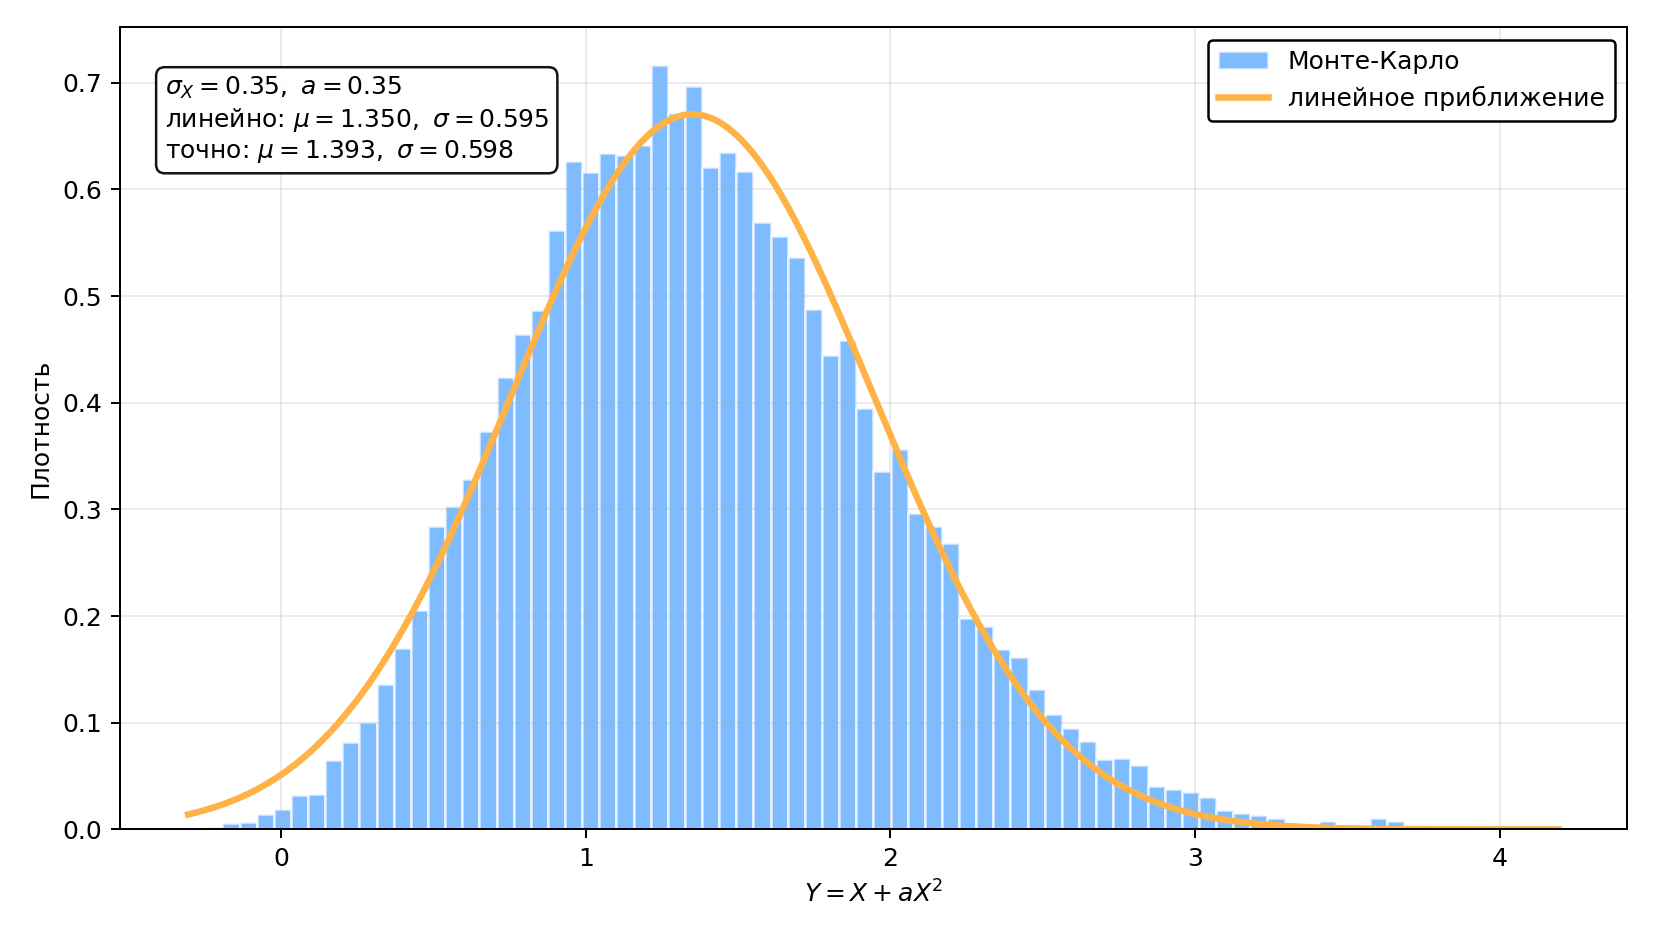
\includegraphics[width=0.74\linewidth,height=\textheight,keepaspectratio,alt={Нелинейное преобразование \$Y=X+aX\^{}2\$}]{assets/figures/error_propagation_nonlinear_default.png}

\end{center}

\noindent\begin{minipage}[c]{\dimexpr\linewidth-30mm\relax}

\textbf{Интерактив}. \textbf{Нелинейное преобразование \(Y=X+aX^2\)}

Меняйте ширину исходного гаусса и коэффициент \(a\). Гистограмма
показывает распределение \(Y\), а гладкая кривая --- линейный прогноз.

\end{minipage}\hfill\begin{minipage}[c]{26mm}\centering

\href{https://neutrinohit.github.io/statistical-analysis-course/ru/book/chapters/06_error_propagation.html\#interactive-error-propagation-nonlinear}{
\includegraphics[width=24mm,height=\textheight,keepaspectratio,alt={QR-код интерактива}]{assets/qr/error-propagation-nonlinear.png}}

\end{minipage}

\end{semanticpdfbox}

На рисунке \ref{fig-error-propagation-nonlinear-strong} показан режим, в
котором кривизна уже существенна на масштабе входного распределения.

\begin{figure}

\centering{

\pandocbounded{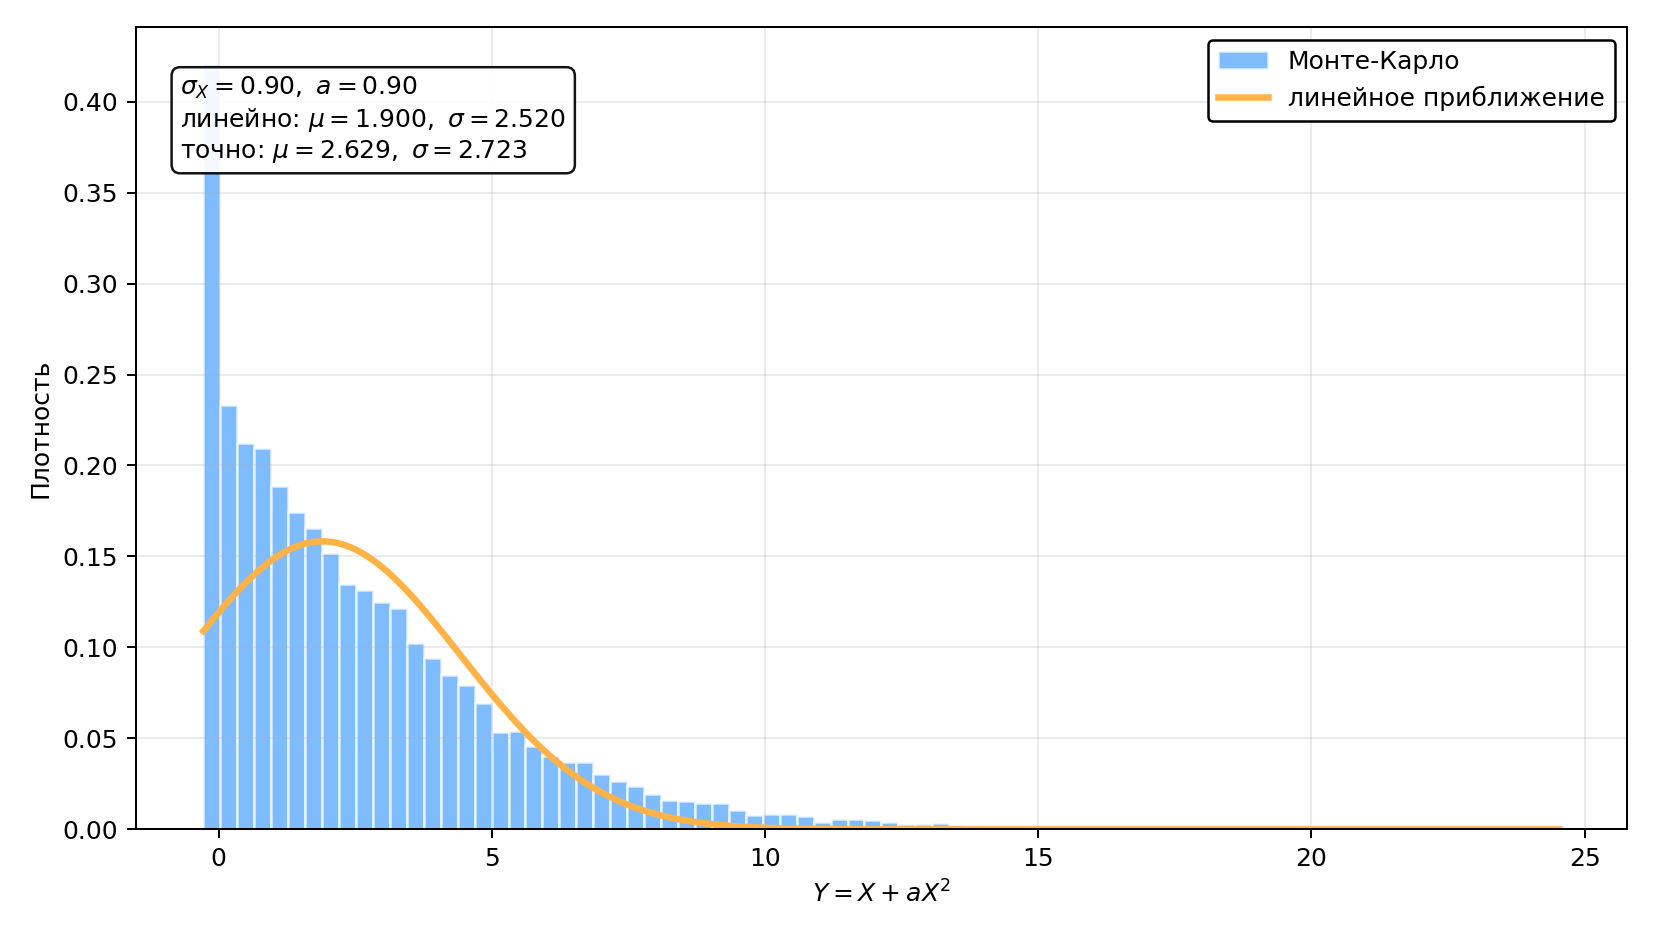
\includegraphics[keepaspectratio]{chapters/../assets/figures/error_propagation_nonlinear_strong.png}}

}

\caption{\label{fig-error-propagation-nonlinear-strong}Распределение
\(Y=X+aX^2\) при \(\sigma_X=0.9\) и \(a=0.9\). Синяя гистограмма
получена методом Монте-Карло, оранжевая кривая показывает гауссово
распределение с параметрами линейного приближения.}

\end{figure}%

Здесь расхождение видно по положению максимума, ширине и длинному
правому хвосту. Запись \(y\pm\sigma_Y\) сохраняет два числа, но уже не
описывает форму распределения. В такой ситуации используют
преобразование полного распределения или численное моделирование.

\section{Разброс оценки стандартного
отклонения}\label{ux440ux430ux437ux431ux440ux43eux441-ux43eux446ux435ux43dux43aux438-ux441ux442ux430ux43dux434ux430ux440ux442ux43dux43eux433ux43e-ux43eux442ux43aux43bux43eux43dux435ux43dux438ux44f}

До сих пор \(\mu\) и \(\sigma\) были известными параметрами
распределения. В эксперименте их оценивают по выборке

\begin{equation}\protect\phantomsection\label{eq-ch6-gaussian-sample-model}{
X_1,\ldots,X_N\sim\mathcal N(\mu,\sigma^2),
}\end{equation}

где измерения независимы. Определим оценки среднего, дисперсии и
стандартного отклонения:

\begin{equation}\protect\phantomsection\label{eq-ch6-sample-mean-estimator}{
\widehat\mu=\overline X
=\frac1N\sum_{k=1}^{N}X_k,
}\end{equation}

\begin{equation}\protect\phantomsection\label{eq-ch6-sample-variance-estimators}{
\widehat{\sigma^2}
=\frac1{N-1}\sum_{k=1}^{N}(X_k-\overline X)^2,
\qquad
\widehat\sigma=\sqrt{\widehat{\sigma^2}}.
}\end{equation}

Если повторить весь эксперимент, выборка изменится вместе со всеми тремя
оценками. Поэтому у \(\widehat\sigma\) есть собственное распределение и
собственная дисперсия.

Для выборочного среднего

\begin{equation}\protect\phantomsection\label{eq-ch6-sample-mean-variance}{
\operatorname{Var}(\widehat\mu)=\frac{\sigma^2}{N}.
}\end{equation}

Параметр \(\sigma^2\) неизвестен, и в оценке дисперсии среднего его
заменяют выборочной дисперсией:

\begin{equation}\protect\phantomsection\label{eq-ch6-estimated-mean-uncertainty}{
\widehat{\operatorname{Var}}(\widehat\mu)
=\frac{\widehat{\sigma^2}}{N},
\qquad
\widehat\sigma_{\widehat\mu}
=\frac{\widehat\sigma}{\sqrt N}.
}\end{equation}

Возникает следующий вопрос: насколько устойчиво значение
\(\widehat\sigma\), найденное по конечной выборке?

\subsection{\texorpdfstring{Почему в выборочной дисперсии стоит
\(N-1\)}{Почему в выборочной дисперсии стоит N-1}}\label{ux43fux43eux447ux435ux43cux443-ux432-ux432ux44bux431ux43eux440ux43eux447ux43dux43eux439-ux434ux438ux441ux43fux435ux440ux441ux438ux438-ux441ux442ux43eux438ux442-n-1}

Введём отклонения от истинного среднего

\begin{equation}\protect\phantomsection\label{eq-ch6-centered-observations}{
Y_k=X_k-\mu.
}\end{equation}

Для независимой выборки с конечной дисперсией

\begin{equation}\protect\phantomsection\label{eq-ch6-centered-first-two-moments}{
\mathbb E[Y_k]=0,
\qquad
\mathbb E[Y_k^2]=\sigma^2.
}\end{equation}

Гауссовость для доказательства несмещённости выборочной дисперсии не
нужна.

\begin{bookderivation}

\subsubsection{Несмещённость выборочной
дисперсии}\label{ux43dux435ux441ux43cux435ux449ux451ux43dux43dux43eux441ux442ux44c-ux432ux44bux431ux43eux440ux43eux447ux43dux43eux439-ux434ux438ux441ux43fux435ux440ux441ux438ux438}

Обозначим две суммы

\begin{equation}\protect\phantomsection\label{eq-ch6-centered-sums-ab}{
A=\sum_{k=1}^{N}Y_k^2,
\qquad
B=\sum_{k=1}^{N}Y_k.
}\end{equation}

Разность выборочного и истинного среднего равна

\begin{equation}\protect\phantomsection\label{eq-ch6-sample-mean-centered-sum}{
\overline X-\mu=\frac{B}{N}.
}\end{equation}

Сумма квадратов отклонений от выборочного среднего принимает вид

\begin{equation}\protect\phantomsection\label{eq-ch6-residual-sum-of-squares}{
\begin{aligned}
T
&=\sum_{k=1}^{N}(X_k-\overline X)^2\\
&=\sum_{k=1}^{N}\left(Y_k-\frac BN\right)^2\\
&=A-\frac{B^2}{N}.
\end{aligned}
}\end{equation}

Независимость и центрирование дают

\begin{equation}\protect\phantomsection\label{eq-ch6-ab-expectations}{
\mathbb E[A]=N\sigma^2,
\qquad
\mathbb E[B^2]=N\sigma^2.
}\end{equation}

Отсюда

\begin{equation}\protect\phantomsection\label{eq-ch6-residual-sum-expectation}{
\mathbb E[T]
=N\sigma^2-\frac1N N\sigma^2
=(N-1)\sigma^2.
}\end{equation}

После деления на \(N-1\)

\begin{equation}\protect\phantomsection\label{eq-ch6-sample-variance-unbiased}{
\boxed{
\mathbb E[\widehat{\sigma^2}]=\sigma^2.
}
}\end{equation}

\end{bookderivation}

Выборочные отклонения связаны условием

\begin{equation}\protect\phantomsection\label{eq-ch6-residuals-constraint}{
\sum_{k=1}^{N}(X_k-\overline X)=0.
}\end{equation}

Одно из \(N\) отклонений определяется через остальные. Поэтому сумма их
квадратов содержит \(N-1\) степеней свободы, и такой же делитель
появляется в несмещённой оценке дисперсии.

\subsection{Дисперсия оценки
дисперсии}\label{ux434ux438ux441ux43fux435ux440ux441ux438ux44f-ux43eux446ux435ux43dux43aux438-ux434ux438ux441ux43fux435ux440ux441ux438ux438}

Теперь понадобится гауссовость. Для центрированной гауссовой величины

\begin{equation}\protect\phantomsection\label{eq-ch6-gaussian-fourth-moment}{
\mathbb E[Y_k^4]=3\sigma^4.
}\end{equation}

Поскольку \(\widehat{\sigma^2}=T/(N-1)\), достаточно найти дисперсию
\(T\).

\begin{bookderivation}

\subsubsection{\texorpdfstring{Вычисление
\(\operatorname{Var}(\widehat{\sigma^2})\)}{Вычисление \textbackslash operatorname\{Var\}(\textbackslash widehat\{\textbackslash sigma\^{}2\})}}\label{ux432ux44bux447ux438ux441ux43bux435ux43dux438ux435-operatornamevarwidehatsigma2}

Из уравнения \ref{eq-ch6-residual-sum-of-squares}

\begin{equation}\protect\phantomsection\label{eq-ch6-residual-sum-square-expanded}{
T^2=A^2-\frac2N AB^2+\frac1{N^2}B^4.
}\end{equation}

Первый момент вычисляется раскрытием квадрата суммы:

\begin{equation}\protect\phantomsection\label{eq-ch6-a-second-moment}{
\begin{aligned}
\mathbb E[A^2]
&=\sum_{k=1}^{N}\mathbb E[Y_k^4]
+2\sum_{i<j}\mathbb E[Y_i^2Y_j^2]\\
&=3N\sigma^4+N(N-1)\sigma^4\\
&=N(N+2)\sigma^4.
\end{aligned}
}\end{equation}

Для смешанного момента выделим одно слагаемое, \(B=Y_i+C_i\), где
\(C_i=\sum_{j\ne i}Y_j\). Величины \(Y_i\) и \(C_i\) независимы,
\(\mathbb E[C_i]=0\) и \(\mathbb E[C_i^2]=(N-1)\sigma^2\). Поэтому

\begin{equation}\protect\phantomsection\label{eq-ch6-one-term-ab2-moment}{
\begin{aligned}
\mathbb E[Y_i^2B^2]
&=\mathbb E[Y_i^2(Y_i+C_i)^2]\\
&=3\sigma^4+(N-1)\sigma^4\\
&=(N+2)\sigma^4,
\end{aligned}
}\end{equation}

и после суммирования по \(i\)

\begin{equation}\protect\phantomsection\label{eq-ch6-ab2-moment}{
\mathbb E[AB^2]=N(N+2)\sigma^4.
}\end{equation}

Сумма \(B\) также гауссова, причём \(\operatorname{Var}(B)=N\sigma^2\).
Её четвёртый момент равен

\begin{equation}\protect\phantomsection\label{eq-ch6-b-fourth-moment}{
\mathbb E[B^4]=3N^2\sigma^4.
}\end{equation}

Подстановка трёх средних в уравнение
\ref{eq-ch6-residual-sum-square-expanded} даёт

\begin{equation}\protect\phantomsection\label{eq-ch6-residual-sum-second-moment}{
\mathbb E[T^2]=(N^2-1)\sigma^4.
}\end{equation}

Вместе с уравнением \ref{eq-ch6-residual-sum-expectation} это приводит к

\begin{equation}\protect\phantomsection\label{eq-ch6-residual-sum-variance}{
\operatorname{Var}(T)
=2(N-1)\sigma^4.
}\end{equation}

Искомая дисперсия оценки равна

\begin{equation}\protect\phantomsection\label{eq-ch6-sample-variance-variance}{
\boxed{
\operatorname{Var}(\widehat{\sigma^2})
=\frac{2\sigma^4}{N-1}.
}
}\end{equation}

\end{bookderivation}

Уравнение \ref{eq-ch6-sample-variance-variance} является точным для
независимой гауссовой выборки. Для другого исходного распределения в
ответ входит его четвёртый центральный момент.

\subsection{Разброс оценки стандартного
отклонения}\label{ux440ux430ux437ux431ux440ux43eux441-ux43eux446ux435ux43dux43aux438-ux441ux442ux430ux43dux434ux430ux440ux442ux43dux43eux433ux43e-ux43eux442ux43aux43bux43eux43dux435ux43dux438ux44f-1}

Оценка \(\widehat\sigma\) связана с \(\widehat{\sigma^2}\) функцией
квадратного корня. Применим к ней формулу
\ref{eq-error-propagation-one-variable} в точке \(\sigma^2\):

\begin{equation}\protect\phantomsection\label{eq-ch6-square-root-derivative}{
f(y)=\sqrt y,
\qquad
f'(\sigma^2)=\frac1{2\sigma}.
}\end{equation}

Получаем

\begin{equation}\protect\phantomsection\label{eq-ch6-standard-deviation-estimator-variance}{
\operatorname{Var}(\widehat\sigma)
\simeq
\frac1{4\sigma^2}
\operatorname{Var}(\widehat{\sigma^2})
=\frac{\sigma^2}{2(N-1)}.
}\end{equation}

Относительный разброс оценки стандартного отклонения равен

\begin{equation}\protect\phantomsection\label{eq-ch6-standard-deviation-relative-spread}{
\boxed{
\frac{\sqrt{\operatorname{Var}(\widehat\sigma)}}{\sigma}
\simeq
\frac1{\sqrt{2(N-1)}}.
}
}\end{equation}

Здесь снова использовано линейное приближение, теперь уже для
квадратного корня. При конечном \(N\) оценка \(\widehat\sigma\) немного
смещена вниз; с ростом выборки смещение исчезает, и формула становится
точнее.

Для относительного разброса около \(10\%\)

\begin{equation}\protect\phantomsection\label{eq-ch6-sample-size-for-ten-percent-sigma}{
\frac1{\sqrt{2(N-1)}}\simeq0.1,
\qquad
N\simeq51.
}\end{equation}

Пятьдесят измерений нужны лишь для того, чтобы сама оценка ширины
флуктуировала примерно на десять процентов. Ширину распределения обычно
измерить труднее, чем его среднее.

\subsection{Десять гауссовских
измерений}\label{interactive-error-propagation-sample-variance}

\begin{semanticpdfbox}[breakable=false]

\begin{center}

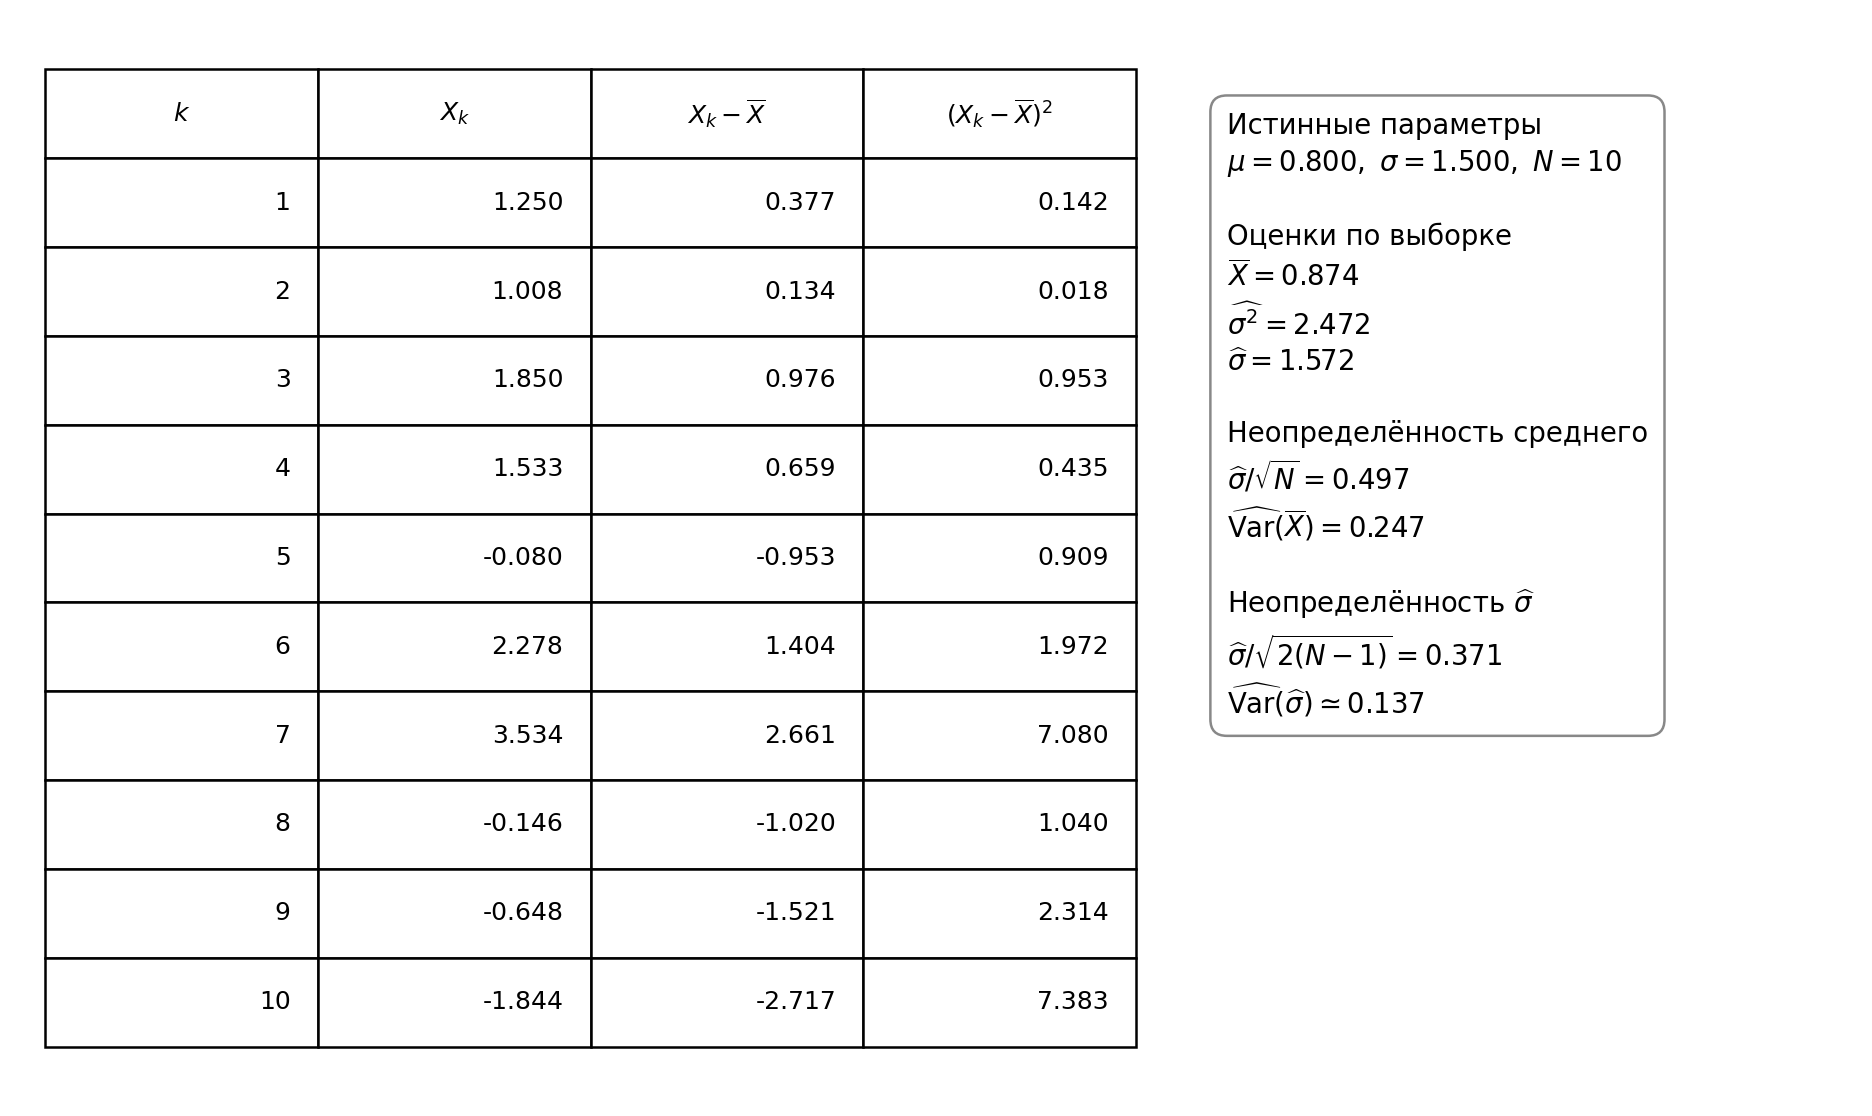
\includegraphics[width=0.74\linewidth,height=\textheight,keepaspectratio,alt={Десять гауссовских измерений}]{assets/figures/error_propagation_sample10.png}

\end{center}

\noindent\begin{minipage}[c]{\dimexpr\linewidth-30mm\relax}

\textbf{Интерактив}. \textbf{Десять гауссовских измерений}

Меняйте параметры распределения и начальное состояние генератора.
Таблица показывает выборку, оценки \(\widehat\mu\),
\(\widehat{\sigma^2}\), \(\widehat\sigma\) и их расчётные
неопределённости.

\end{minipage}\hfill\begin{minipage}[c]{26mm}\centering

\href{https://neutrinohit.github.io/statistical-analysis-course/ru/book/chapters/06_error_propagation.html\#interactive-error-propagation-sample-variance}{
\includegraphics[width=24mm,height=\textheight,keepaspectratio,alt={QR-код интерактива}]{assets/qr/error-propagation-sample-variance.png}}

\end{minipage}

\end{semanticpdfbox}

Десять чисел выглядят вполне убедительно, пока рядом не написаны
истинные параметры. Новая выборка даёт другие \(\widehat\mu\) и
\(\widehat\sigma\). Формулы выше описывают разброс этих результатов в
серии повторений.

\section{Несколько измеряемых
величин}\label{ux43dux435ux441ux43aux43eux43bux44cux43aux43e-ux438ux437ux43cux435ux440ux44fux435ux43cux44bux445-ux432ux435ux43bux438ux447ux438ux43d}

В задаче о сечении использовались три входные величины. Теперь выведем
формулу, которая учитывает их совместные флуктуации.

\subsection{Ковариация и ошибка
суммы}\label{ux43aux43eux432ux430ux440ux438ux430ux446ux438ux44f-ux438-ux43eux448ux438ux431ux43aux430-ux441ux443ux43cux43cux44b}

Ковариация \(X\) и \(Y\) равна

\begin{equation}\protect\phantomsection\label{eq-ch6-covariance-definition}{
\operatorname{cov}(X,Y)
=\mathbb E[(X-\mu_X)(Y-\mu_Y)].
}\end{equation}

Для суммы \(S=X+Y\)

\begin{equation}\protect\phantomsection\label{eq-ch6-sum-variance-with-covariance}{
\operatorname{Var}(S)
=\sigma_X^2+\sigma_Y^2
+2\operatorname{cov}(X,Y).
}\end{equation}

Коэффициент корреляции убирает размерность ковариации:

\begin{equation}\protect\phantomsection\label{eq-ch6-correlation-coefficient}{
\rho_{XY}
=\frac{\operatorname{cov}(X,Y)}{\sigma_X\sigma_Y},
\qquad
-1\le\rho_{XY}\le1.
}\end{equation}

Для суммы и разности

\begin{equation}\protect\phantomsection\label{eq-ch6-sum-difference-uncertainty}{
\sigma_{X\pm Y}^2
=\sigma_X^2+\sigma_Y^2
\pm2\rho_{XY}\sigma_X\sigma_Y.
}\end{equation}

Положительная корреляция увеличивает ошибку суммы и уменьшает ошибку
разности. При отрицательной корреляции знаки меняются. Складывать ошибки
в квадратуре можно при нулевой ковариации.

Независимость влечёт \(\rho_{XY}=0\). Обратное утверждение для
произвольного распределения неверно: при нулевой корреляции нелинейная
зависимость может сохраняться.

\subsection{Оценка корреляции по
выборке}\label{ux43eux446ux435ux43dux43aux430-ux43aux43eux440ux440ux435ux43bux44fux446ux438ux438-ux43fux43e-ux432ux44bux431ux43eux440ux43aux435}

Пусть получены \(N\) независимых пар \((x_k,y_k)\) из одного совместного
распределения. Выборочная ковариация равна

\begin{equation}\protect\phantomsection\label{eq-ch6-sample-covariance}{
\widehat{\operatorname{cov}}(X,Y)
=\frac1{N-1}\sum_{k=1}^{N}
(x_k-\overline x)(y_k-\overline y),
}\end{equation}

а выборочный коэффициент корреляции ---

\begin{equation}\protect\phantomsection\label{eq-ch6-sample-correlation}{
\widehat\rho
=\frac{\widehat{\operatorname{cov}}(X,Y)}{s_Xs_Y}.
}\end{equation}

При небольшом \(N\) значение \(\widehat\rho\) заметно меняется от
выборки к выборке. В детекторных задачах ковариации получают также из
моделирования, калибровочных данных и вариаций систематических
параметров.

\subsection{Общая формула
распространения}\label{ux43eux431ux449ux430ux44f-ux444ux43eux440ux43cux443ux43bux430-ux440ux430ux441ux43fux440ux43eux441ux442ux440ux430ux43dux435ux43dux438ux44f}

Пусть

\begin{equation}\protect\phantomsection\label{eq-ch6-multivariable-transformation}{
F=f(X_1,\ldots,X_n),
}\end{equation}

а средние входных величин образуют вектор
\(\boldsymbol\mu=(\mu_1,\ldots,\mu_n)^{\mathsf T}\). Первый порядок
разложения имеет вид

\begin{equation}\protect\phantomsection\label{eq-ch6-multivariable-linearization}{
F-\mathbb E[F]
\simeq
\sum_{i=1}^{n}
\left.
\frac{\partial f}{\partial x_i}
\right|_{\boldsymbol\mu}
(X_i-\mu_i).
}\end{equation}

\begin{bookderivation}

\subsubsection{Дисперсия функции нескольких
переменных}\label{ux434ux438ux441ux43fux435ux440ux441ux438ux44f-ux444ux443ux43dux43aux446ux438ux438-ux43dux435ux441ux43aux43eux43bux44cux43aux438ux445-ux43fux435ux440ux435ux43cux435ux43dux43dux44bux445}

Обозначим производные в точке \(\boldsymbol\mu\) через

\begin{equation}\protect\phantomsection\label{eq-ch6-gradient-components}{
g_i=
\left.
\frac{\partial f}{\partial x_i}
\right|_{\boldsymbol\mu}.
}\end{equation}

После возведения линейного разложения в квадрат

\begin{equation}\protect\phantomsection\label{eq-ch6-multivariable-variance-derivation}{
\begin{aligned}
\operatorname{Var}(F)
&\simeq
\mathbb E\!\left[
\left(\sum_i g_i(X_i-\mu_i)\right)
\left(\sum_j g_j(X_j-\mu_j)\right)
\right]\\
&=\sum_{i,j}g_i
\operatorname{cov}(X_i,X_j)g_j.
\end{aligned}
}\end{equation}

Итак,

\begin{equation}\protect\phantomsection\label{eq-error-propagation-covariance}{
\boxed{
\operatorname{Var}(F)
\simeq
\sum_{i,j}
\frac{\partial f}{\partial x_i}
\operatorname{cov}(X_i,X_j)
\frac{\partial f}{\partial x_j}.
}
}\end{equation}

\end{bookderivation}

Все производные в уравнении \ref{eq-error-propagation-covariance}
вычисляются в одной точке \(\boldsymbol\mu\). На практике неизвестные
средние заменяют полученными центральными значениями.

Для двух переменных формула разворачивается в три слагаемых:

\begin{equation}\protect\phantomsection\label{eq-ch6-two-variable-error-propagation}{
\begin{aligned}
\sigma_F^2\simeq{}
&\left(\frac{\partial f}{\partial x}\right)^2\sigma_X^2
+\left(\frac{\partial f}{\partial y}\right)^2\sigma_Y^2\\
&+2\rho_{XY}
\frac{\partial f}{\partial x}
\frac{\partial f}{\partial y}
\sigma_X\sigma_Y.
\end{aligned}
}\end{equation}

Знак корреляционного вклада определяется одновременно знаком
\(\rho_{XY}\) и знаками двух производных.

\subsection{Корреляционный вклад в
дисперсию}\label{interactive-error-propagation-correlation}

\begin{semanticpdfbox}[breakable=false]

\begin{center}

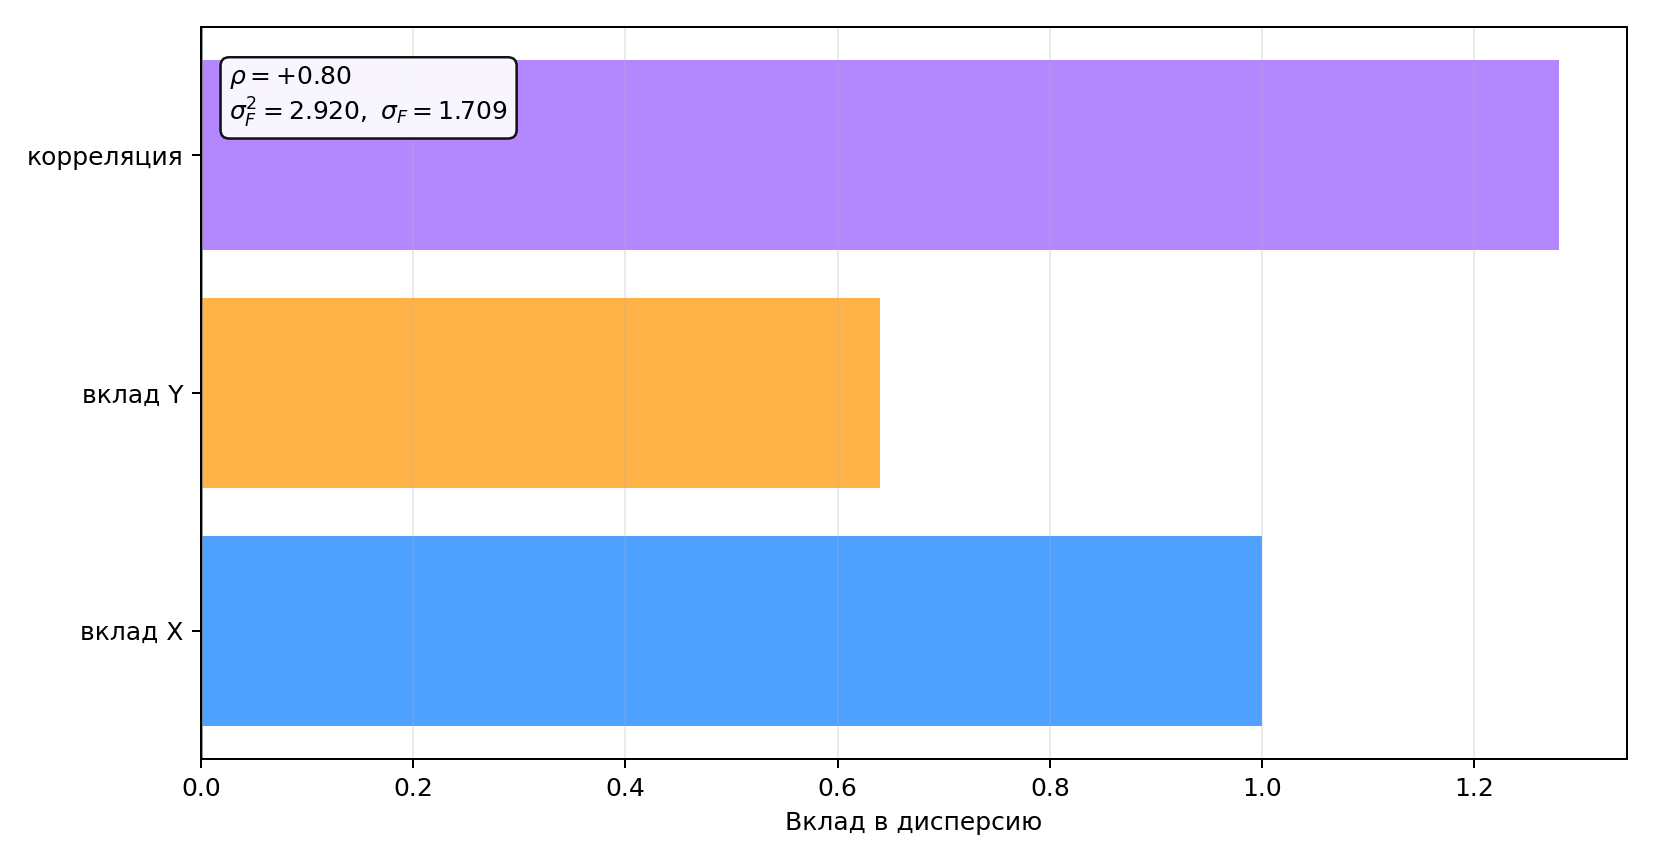
\includegraphics[width=0.74\linewidth,height=\textheight,keepaspectratio,alt={Корреляционный вклад в дисперсию}]{assets/figures/error_propagation_corr_positive.png}

\end{center}

\noindent\begin{minipage}[c]{\dimexpr\linewidth-30mm\relax}

\textbf{Интерактив}. \textbf{Корреляционный вклад в дисперсию}

Меняйте производные, стандартные отклонения и \(\rho\). Три полосы
показывают два диагональных и один корреляционный вклад в
\(\sigma_F^2\).

\end{minipage}\hfill\begin{minipage}[c]{26mm}\centering

\href{https://neutrinohit.github.io/statistical-analysis-course/ru/book/chapters/06_error_propagation.html\#interactive-error-propagation-correlation}{
\includegraphics[width=24mm,height=\textheight,keepaspectratio,alt={QR-код интерактива}]{assets/qr/error-propagation-correlation.png}}

\end{minipage}

\end{semanticpdfbox}

На рисунке \ref{fig-error-propagation-negative-correlation} производные
имеют одинаковый знак, а корреляция отрицательна. Корреляционный член
вычитается из двух положительных вкладов.

\begin{figure}

\centering{

\pandocbounded{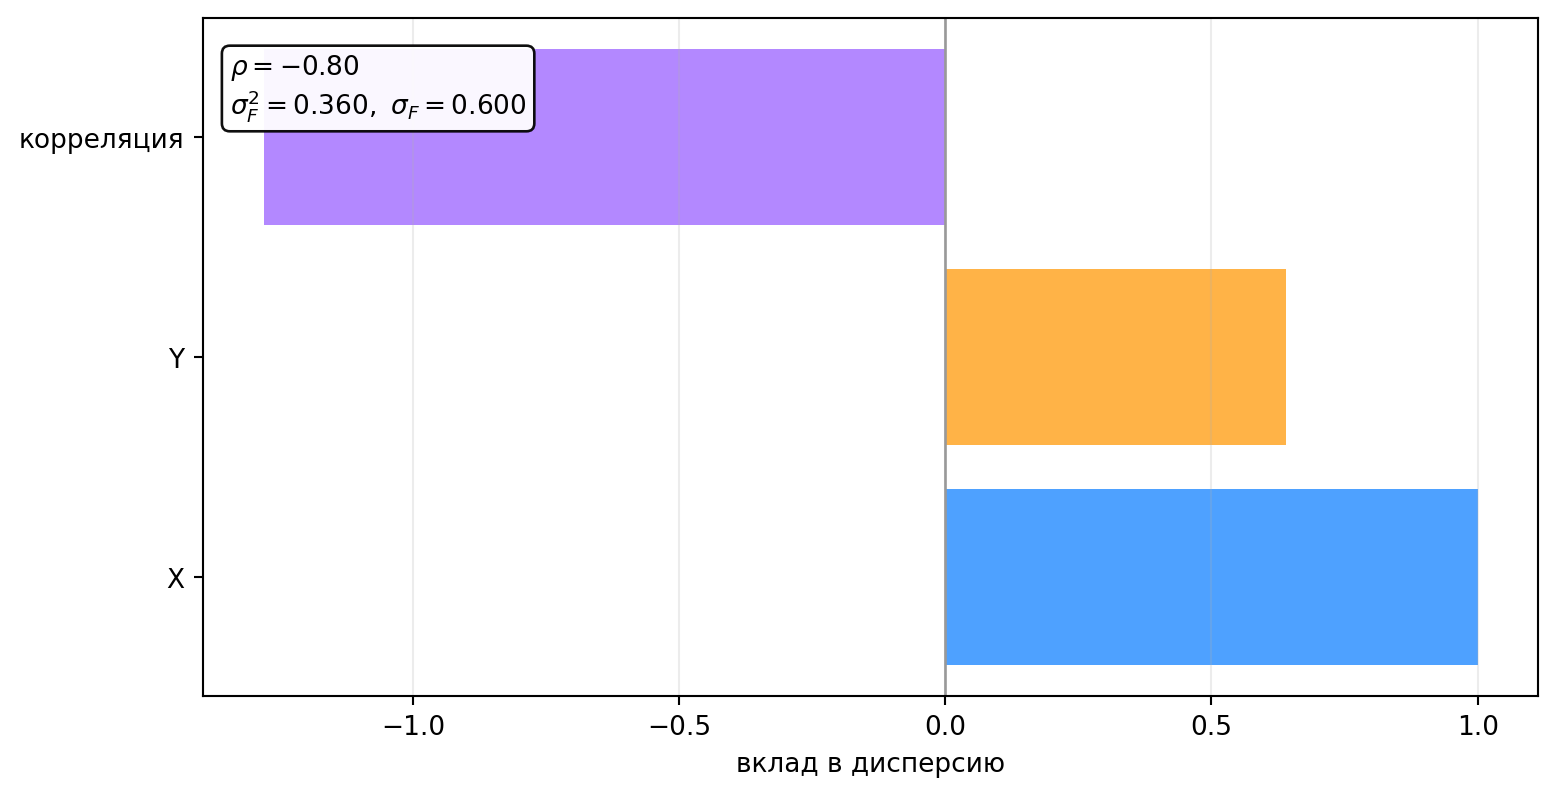
\includegraphics[keepaspectratio]{chapters/../assets/figures/error_propagation_corr_negative.png}}

}

\caption{\label{fig-error-propagation-negative-correlation}Вклады в
дисперсию функции двух переменных при
\(\partial f/\partial x=\partial f/\partial y=1\), \(\sigma_X=1\),
\(\sigma_Y=0.8\) и \(\rho=-0.8\). Отрицательный корреляционный член
уменьшает полную дисперсию до \(0.36\).}

\end{figure}%

\subsection{Отношение двух
величин}\label{ux43eux442ux43dux43eux448ux435ux43dux438ux435-ux434ux432ux443ux445-ux432ux435ux43bux438ux447ux438ux43d}

Для

\begin{equation}\protect\phantomsection\label{eq-ch6-ratio-definition}{
R=\frac XY
}\end{equation}

две производные равны

\begin{equation}\protect\phantomsection\label{eq-ch6-ratio-derivatives}{
\frac{\partial R}{\partial X}=\frac1Y,
\qquad
\frac{\partial R}{\partial Y}=-\frac{X}{Y^2}.
}\end{equation}

Линейная относительная неопределённость составляет

\begin{equation}\protect\phantomsection\label{eq-ch6-ratio-relative-uncertainty}{
\boxed{
\left(\frac{\sigma_R}{R}\right)^2
\simeq
\left(\frac{\sigma_X}{X}\right)^2
+\left(\frac{\sigma_Y}{Y}\right)^2
-2\rho_{XY}
\frac{\sigma_X}{X}
\frac{\sigma_Y}{Y}.
}
}\end{equation}

Производные по числителю и знаменателю имеют разные знаки. Поэтому
положительная корреляция уменьшает ошибку отношения. Формула требует,
чтобы знаменатель с большой вероятностью оставался вдали от нуля. В
главе 5 мы видели крайний случай: отношение двух независимых стандартных
гауссовых величин имеет распределение Коши.

\subsection{Возвращение к
сечению}\label{ux432ux43eux437ux432ux440ux430ux449ux435ux43dux438ux435-ux43a-ux441ux435ux447ux435ux43dux438ux44e}

Для функции

\begin{equation}\protect\phantomsection\label{eq-ch6-cross-section-function}{
\widehat\sigma_{\mathrm{proc}}(N,\varepsilon,L)
=\frac{N}{\varepsilon L}
}\end{equation}

производные удобно записать через само сечение:

\begin{equation}\protect\phantomsection\label{eq-ch6-cross-section-derivatives}{
\frac{\partial\widehat\sigma_{\mathrm{proc}}}{\partial N}
=\frac{\widehat\sigma_{\mathrm{proc}}}{N},
\qquad
\frac{\partial\widehat\sigma_{\mathrm{proc}}}{\partial\varepsilon}
=-\frac{\widehat\sigma_{\mathrm{proc}}}{\varepsilon},
\qquad
\frac{\partial\widehat\sigma_{\mathrm{proc}}}{\partial L}
=-\frac{\widehat\sigma_{\mathrm{proc}}}{L}.
}\end{equation}

Общая относительная дисперсия равна

\begin{equation}\protect\phantomsection\label{eq-ch6-cross-section-full-uncertainty}{
\begin{aligned}
\left(
\frac{\sigma_{\widehat\sigma_{\mathrm{proc}}}}
     {\widehat\sigma_{\mathrm{proc}}}
\right)^2
\simeq{}
&\frac{\sigma_N^2}{N^2}
+\frac{\sigma_\varepsilon^2}{\varepsilon^2}
+\frac{\sigma_L^2}{L^2}\\
&-2\frac{\operatorname{cov}(N,\varepsilon)}{N\varepsilon}
-2\frac{\operatorname{cov}(N,L)}{NL}
+2\frac{\operatorname{cov}(\varepsilon,L)}{\varepsilon L}.
\end{aligned}
}\end{equation}

При нулевых ковариациях остаётся формула, использованная в начале главы.
Знаки трёх ковариационных членов следуют из знаков производных, поэтому
механическое сложение всех вкладов в квадратуре может дать неверный
ответ.

\section{Ковариационная
матрица}\label{ux43aux43eux432ux430ux440ux438ux430ux446ux438ux43eux43dux43dux430ux44f-ux43cux430ux442ux440ux438ux446ux430}

Для случайного вектора

\begin{equation}\protect\phantomsection\label{eq-ch6-random-vector-definition}{
\mathbf X=(X_1,\ldots,X_n)^{\mathsf T}
}\end{equation}

определим матрицу

\begin{equation}\protect\phantomsection\label{eq-ch6-covariance-matrix-definition}{
(\mathbf V_X)_{ij}
=\operatorname{cov}(X_i,X_j).
}\end{equation}

В двумерном случае

\begin{equation}\protect\phantomsection\label{eq-ch6-two-dimensional-covariance-matrix}{
\mathbf V_X=
\begin{pmatrix}
\sigma_X^2 & \rho\sigma_X\sigma_Y\\
\rho\sigma_X\sigma_Y & \sigma_Y^2
\end{pmatrix}.
}\end{equation}

Ковариационная матрица симметрична. На диагонали стоят дисперсии, а для
любого вектора \(\mathbf a\)

\begin{equation}\protect\phantomsection\label{eq-ch6-covariance-positive-semidefinite}{
\mathbf a^{\mathsf T}\mathbf V_X\mathbf a
=\operatorname{Var}(\mathbf a^{\mathsf T}\mathbf X)
\ge0.
}\end{equation}

Последнее равенство объясняет требование положительной
полуопределённости: никакая линейная комбинация измерений не может иметь
отрицательную дисперсию. Матрица с нарушенным условием не описывает
совместное распределение случайных величин.

\subsection{Матричная запись распространения
ошибки}\label{ux43cux430ux442ux440ux438ux447ux43dux430ux44f-ux437ux430ux43fux438ux441ux44c-ux440ux430ux441ux43fux440ux43eux441ux442ux440ux430ux43dux435ux43dux438ux44f-ux43eux448ux438ux431ux43aux438}

Соберём производные скалярной функции в градиент

\begin{equation}\protect\phantomsection\label{eq-ch6-gradient-vector}{
\mathbf g=
\left.
\nabla f
\right|_{\boldsymbol\mu}
=
\begin{pmatrix}
\partial f/\partial x_1\\
\vdots\\
\partial f/\partial x_n
\end{pmatrix}_{\boldsymbol\mu}.
}\end{equation}

Уравнение \ref{eq-error-propagation-covariance} записывается одной
строкой:

\begin{equation}\protect\phantomsection\label{eq-ch6-gradient-covariance-form}{
\boxed{
\sigma_F^2\simeq
\mathbf g^{\mathsf T}\mathbf V_X\mathbf g.
}
}\end{equation}

Пусть выходных величин несколько,

\begin{equation}\protect\phantomsection\label{eq-ch6-vector-transformation}{
\mathbf Y=\mathbf f(\mathbf X),
}\end{equation}

а матрица Якоби имеет элементы

\begin{equation}\protect\phantomsection\label{eq-ch6-jacobian-definition}{
J_{ai}=
\left.
\frac{\partial f_a}{\partial x_i}
\right|_{\boldsymbol\mu}.
}\end{equation}

Тогда

\begin{equation}\protect\phantomsection\label{eq-ch6-covariance-matrix-propagation}{
\boxed{
\mathbf V_Y
\simeq
\mathbf J\mathbf V_X\mathbf J^{\mathsf T}.
}
}\end{equation}

Для линейного преобразования матрица \(\mathbf J\) постоянна и уравнение
\ref{eq-ch6-covariance-matrix-propagation} является точным. Для
нелинейной функции это первый порядок разложения около
\(\boldsymbol\mu\).

\subsection{Сумма и
разность}\label{ux441ux443ux43cux43cux430-ux438-ux440ux430ux437ux43dux43eux441ux442ux44c}

Возьмём

\begin{equation}\protect\phantomsection\label{eq-ch6-sum-difference-vector-transformation}{
\mathbf X=
\begin{pmatrix}X\\Y\end{pmatrix},
\qquad
\mathbf U=
\begin{pmatrix}S\\D\end{pmatrix}
=
\begin{pmatrix}X+Y\\X-Y\end{pmatrix}.
}\end{equation}

Матрица Якоби равна

\begin{equation}\protect\phantomsection\label{eq-ch6-sum-difference-jacobian}{
\mathbf J=
\begin{pmatrix}
1&1\\
1&-1
\end{pmatrix}.
}\end{equation}

Для входной матрицы

\begin{equation}\protect\phantomsection\label{eq-ch6-sum-difference-input-covariance}{
\mathbf V_X=
\begin{pmatrix}
\sigma_X^2&\sigma_{XY}\\
\sigma_{XY}&\sigma_Y^2
\end{pmatrix}
}\end{equation}

получаем

\begin{equation}\protect\phantomsection\label{eq-ch6-sum-difference-output-covariance}{
\mathbf V_U
=\mathbf J\mathbf V_X\mathbf J^{\mathsf T}
=
\begin{pmatrix}
\sigma_X^2+\sigma_Y^2+2\sigma_{XY}
&\sigma_X^2-\sigma_Y^2\\
\sigma_X^2-\sigma_Y^2
&\sigma_X^2+\sigma_Y^2-2\sigma_{XY}
\end{pmatrix}.
}\end{equation}

Диагональные элементы воспроизводят ошибки суммы и разности.
Внедиагональный элемент даёт

\begin{equation}\protect\phantomsection\label{eq-ch6-sum-difference-covariance}{
\operatorname{cov}(S,D)=\sigma_X^2-\sigma_Y^2.
}\end{equation}

При \(\sigma_X=\sigma_Y\) сумма и разность некоррелированы даже при
\(\sigma_{XY}\ne0\). В следующей главе мы увидим геометрический смысл
этого результата на двумерном гауссовом распределении.

\begin{bookchaptersummary}[Итоги главы]

\begin{itemize}
\tightlist
\item
  При малой входной неопределённости функция заменяется касательной, и
  для одной переменной \(\sigma_Y\simeq|f'(\mu_X)|\sigma_X\).
\item
  Выборочная дисперсия с делителем \(N-1\) является несмещённой. Для
  гауссовой выборки её дисперсия равна \(2\sigma^4/(N-1)\).
\item
  Корреляции входят в ошибку результата со знаками, заданными
  производными. Квадратурная сумма применима при нулевых ковариациях.
\item
  Ковариационная матрица преобразуется по закону
  \(\mathbf V_Y\simeq\mathbf J\mathbf V_X\mathbf J^{\mathsf T}\); для
  линейной функции это равенство точное.
\end{itemize}

\end{bookchaptersummary}

\section{Задачи}\label{ux437ux430ux434ux430ux447ux438-5}

\begin{semanticpdfbox}[colback=BookCoralSoft,borderline west={1.2mm}{0pt}{BookCoral},breakable=false]

\noindent{\sffamily\bfseries\fontsize{11.2}{13.5}\selectfont Задача 1. Радиус и площадь круга}\par\nopagebreak[4]\vspace{1.2mm}

Измеренный радиус круга равен \[
R=(10.0\pm0.3)\ \text{см}.
\]

\begin{enumerate}
\def\labelenumi{\arabic{enumi}.}
\tightlist
\item
  Найдите площадь \(S=\pi R^2\) и её ошибку в линейном приближении.
\item
  Сравните относительные ошибки \(S\) и \(R\).
\item
  Оцените поправку к математическому ожиданию площади, возникающую из-за
  квадратичности функции.
\end{enumerate}

\end{semanticpdfbox}

\begin{semanticpdfbox}[colback=BookCoralSoft,borderline west={1.2mm}{0pt}{BookCoral},breakable=false]

\noindent{\sffamily\bfseries\fontsize{11.2}{13.5}\selectfont Задача 2. Сумма и разность коррелированных величин}\par\nopagebreak[4]\vspace{1.2mm}

Пусть \[
\sigma_X=2,
\qquad
\sigma_Y=3,
\qquad
\rho_{XY}=0.8.
\]

Вычислите ошибки: \[
S=X+Y,
\qquad
D=X-Y.
\]

Повторите вычисление для \(\rho_{XY}=-0.8\) и объясните изменение
результата.

\end{semanticpdfbox}

\begin{semanticpdfbox}[colback=BookCoralSoft,borderline west={1.2mm}{0pt}{BookCoral},breakable=false]

\noindent{\sffamily\bfseries\fontsize{11.2}{13.5}\selectfont Задача 3. Ошибка отношения}\par\nopagebreak[4]\vspace{1.2mm}

Эффективность определяется отношением \[
\varepsilon=\frac{N_{\mathrm{selected}}}{N_{\mathrm{total}}}.
\]

\begin{enumerate}
\def\labelenumi{\arabic{enumi}.}
\tightlist
\item
  Выведите линейную формулу для \(\sigma_\varepsilon\), предполагая
  известные \(\sigma_{\mathrm{selected}}\), \(\sigma_{\mathrm{total}}\)
  и корреляцию \(\rho\).
\item
  Объясните, почему предположение о независимости числителя и
  знаменателя обычно неверно.
\item
  Сравните ответы для \(\rho=0\) и \(\rho>0\).
\end{enumerate}

\end{semanticpdfbox}

\begin{semanticpdfbox}[colback=BookCoralSoft,borderline west={1.2mm}{0pt}{BookCoral},breakable=false]

\noindent{\sffamily\bfseries\fontsize{11.2}{13.5}\selectfont Задача 4. Преобразование ковариационной матрицы}\par\nopagebreak[4]\vspace{1.2mm}

Пусть \[
\mathbf X=
\begin{pmatrix}X\\Y\end{pmatrix},
\qquad
V_X=
\begin{pmatrix}
4&1.2\\
1.2&1
\end{pmatrix}.
\]

Для новых величин \[
S=X+Y,
\qquad
D=X-Y
\] найдите:

\begin{enumerate}
\def\labelenumi{\arabic{enumi}.}
\tightlist
\item
  матрицу Якоби;
\item
  ковариационную матрицу \(V_{SD}\);
\item
  коэффициент корреляции между \(S\) и \(D\).
\end{enumerate}

\end{semanticpdfbox}

\begin{semanticpdfbox}[colback=BookCoralSoft,borderline west={1.2mm}{0pt}{BookCoral},breakable=false]

\noindent{\sffamily\bfseries\fontsize{11.2}{13.5}\selectfont Задача 5. Проверка линейного приближения}\par\nopagebreak[4]\vspace{1.2mm}

Пусть \[
X\sim\mathrm N(1,\sigma_X^2),
\qquad
Y=X+aX^2.
\]

\begin{enumerate}
\def\labelenumi{\arabic{enumi}.}
\tightlist
\item
  Получите линейную оценку \(\sigma_Y\).
\item
  Выведите точные \(\mathbb E[Y]\) и \(\operatorname{Var}(Y)\).
\item
  Сгенерируйте не менее \(10^5\) значений \(X\) и сравните выборочные
  моменты \(Y\) с точным и линейным результатами.
\item
  На сетке \(0\le a\le1\) и \(0.05\le\sigma_X\le1\) найдите область, в
  которой линейная оценка стандартного отклонения отличается от точной
  менее чем на \(5\%\).
\end{enumerate}

\end{semanticpdfbox}

\section*{Литература}\label{ux43bux438ux442ux435ux440ux430ux442ux443ux440ux430-5}
\addcontentsline{toc}{section}{Литература}

\markright{Литература}

\protect\phantomsection\label{refs}
\begin{CSLReferences}{0}{0}
\bibitem[\citeproctext]{ref-jcgm2008gum}
{[}1{]} Joint Committee for Guides in Metrology. Evaluation of
Measurement Data---Guide to the Expression of Uncertainty in
Measurement. 2008.
doi:\href{https://doi.org/10.59161/JCGM100-2008E}{10.59161/JCGM100-2008E}.

\end{CSLReferences}

\chapter{Двумерное гауссово
распределение}\label{ux434ux432ux443ux43cux435ux440ux43dux43eux435-ux433ux430ux443ux441ux441ux43eux432ux43e-ux440ux430ux441ux43fux440ux435ux434ux435ux43bux435ux43dux438ux435}

\bookchapteropeningcontents

\begin{bookchapteropening}[Аннотация]

Совместное распределение двух измеряемых величин содержит больше
информации, чем две ошибки, выписанные по отдельности. Ковариационная
матрица задаёт масштаб и направление флуктуаций, а её обратная матрица
позволяет измерить расстояние от точки до среднего. В этой главе мы
построим двумерный гаусс, разберём вероятностные эллипсы и применим
полную ковариацию к объединению измерений и восстановлению инвариантной
массы.

\end{bookchapteropening}

\section{Физическая задача: два показания
калориметра}\label{ux444ux438ux437ux438ux447ux435ux441ux43aux430ux44f-ux437ux430ux434ux430ux447ux430-ux434ux432ux430-ux43fux43eux43aux430ux437ux430ux43dux438ux44f-ux43aux430ux43bux43eux440ux438ux43cux435ux442ux440ux430}

Рассмотрим ансамбль измерений событий с одной и той же кинематикой.
Истинные энергии двух фотонов равны \(60\) и \(40\) ГэВ. Будем считать,
что шкала энергии откалибрована без смещения, а отклик калориметра
приближённо гауссов. Тогда средний вектор измеренных энергий равен

\begin{equation}\protect\phantomsection\label{eq-ch7-calorimeter-mean}{
\boldsymbol\mu=
\begin{pmatrix}
60\\
40
\end{pmatrix}\ \text{ГэВ}.
}\end{equation}

Дисперсии измеренных энергий и их ковариация собраны в матрицу

\begin{equation}\protect\phantomsection\label{eq-ch7-calorimeter-covariance}{
V=
\begin{pmatrix}
1.44 & 0.36\\
0.36 & 1.00
\end{pmatrix}\ \text{ГэВ}^2.
}\end{equation}

Вне диагонали стоит положительное число: часть ошибки у двух энергий
общая. Например, обе зависят от одной калибровки шкалы энергии.

Пусть в одном событии получено

\begin{equation}\protect\phantomsection\label{eq-ch7-calorimeter-measurement}{
\mathbf x=
\begin{pmatrix}
61.2\\
41.0
\end{pmatrix}\ \text{ГэВ}.
}\end{equation}

Каждая энергия отличается от среднего ровно на своё стандартное
отклонение. Этого ещё недостаточно, чтобы оценить совместное отклонение.
Для него нужна квадратичная форма

\begin{equation}\protect\phantomsection\label{eq-ch7-calorimeter-mahalanobis}{
D^2=(\mathbf x-\boldsymbol\mu)^{\mathsf T}
V^{-1}(\mathbf x-\boldsymbol\mu)=1.54.
}\end{equation}

Число \(D^2\) безразмерно. Оно учитывает и масштабы двух ошибок, и
направление, в котором они коррелируют. Контур, проходящий через нашу
точку, охватывает около \(54\%\) двумерного гауссова распределения. Для
области с вероятностью \(68.3\%\) потребуется \(D^2\leq2.30\).

Откуда взялись эти числа и почему привычное условие \(D^2\leq1\) здесь
даёт не \(68.3\%\), а только \(39.3\%\)? Для ответа надо построить
двумерный гаусс и посмотреть на геометрию его ковариационной матрицы.

\section{От двух одномерных гауссов к
двумерному}\label{ux43eux442-ux434ux432ux443ux445-ux43eux434ux43dux43eux43cux435ux440ux43dux44bux445-ux433ux430ux443ux441ux441ux43eux432-ux43a-ux434ux432ux443ux43cux435ux440ux43dux43eux43cux443}

\subsection{Независимые
величины}\label{ux43dux435ux437ux430ux432ux438ux441ux438ux43cux44bux435-ux432ux435ux43bux438ux447ux438ux43dux44b}

Пусть

\begin{equation}\protect\phantomsection\label{eq-ch7-independent-marginals}{
X\sim\mathcal N(\mu_X,\sigma_X^2),
\qquad
Y\sim\mathcal N(\mu_Y,\sigma_Y^2)
}\end{equation}

и \(X\) и \(Y\) независимы. Совместная плотность равна произведению двух
одномерных плотностей:

\begin{equation}\protect\phantomsection\label{eq-ch7-independent-density}{
f(x,y)=
\frac{1}{2\pi\sigma_X\sigma_Y}
\exp\!\left[-\frac12\left(
\frac{(x-\mu_X)^2}{\sigma_X^2}
+\frac{(y-\mu_Y)^2}{\sigma_Y^2}
\right)\right].
}\end{equation}

Введём безразмерные отклонения

\begin{equation}\protect\phantomsection\label{eq-ch7-standardized-coordinates}{
u=\frac{x-\mu_X}{\sigma_X},
\qquad
v=\frac{y-\mu_Y}{\sigma_Y}.
}\end{equation}

Плотность постоянна при постоянном значении

\begin{equation}\protect\phantomsection\label{eq-ch7-independent-contour}{
u^2+v^2=c.
}\end{equation}

В координатах \((u,v)\) это окружность. В исходных координатах
получается эллипс с полуосями \(\sqrt c\,\sigma_X\) и
\(\sqrt c\,\sigma_Y\). Его оси совпадают с координатными: отклонение
\(X\) ничего не сообщает об отклонении \(Y\).

\subsection{Корреляция поворачивает
эллипс}\label{ux43aux43eux440ux440ux435ux43bux44fux446ux438ux44f-ux43fux43eux432ux43eux440ux430ux447ux438ux432ux430ux435ux442-ux44dux43bux43bux438ux43fux441}

Ковариационная матрица двух величин имеет вид

\begin{equation}\protect\phantomsection\label{eq-ch7-two-dimensional-covariance}{
V=
\begin{pmatrix}
\sigma_X^2 & \rho\sigma_X\sigma_Y\\
\rho\sigma_X\sigma_Y & \sigma_Y^2
\end{pmatrix},
\qquad |\rho|<1.
}\end{equation}

Смешанный член в совместной плотности появляется вместе с корреляцией:

\begin{equation}\protect\phantomsection\label{eq-ch7-correlated-density}{
f(x,y)=
\frac{1}{2\pi\sigma_X\sigma_Y\sqrt{1-\rho^2}}
\exp\!\left[-\frac12
\frac{u^2-2\rho uv+v^2}{1-\rho^2}
\right].
}\end{equation}

При \(\rho=0\) уравнение \ref{eq-ch7-correlated-density} переходит в
произведение двух одномерных гауссов. При положительной корреляции
большие значения \(X\) чаще сопровождаются большими значениями \(Y\),
поэтому эллипс наклонён вверх. Отрицательная корреляция меняет
направление наклона.

Предел \(|\rho|=1\) в формулу плотности не входит. В этом случае
определитель ковариационной матрицы обращается в нуль, а случайные точки
лежат на прямой. Двумерной плотности относительно площади уже нет.

\subsection{Обратная ковариационная
матрица}\label{ux43eux431ux440ux430ux442ux43dux430ux44f-ux43aux43eux432ux430ux440ux438ux430ux446ux438ux43eux43dux43dux430ux44f-ux43cux430ux442ux440ux438ux446ux430}

Для матрицы \ref{eq-ch7-two-dimensional-covariance}

\begin{equation}\protect\phantomsection\label{eq-ch7-covariance-determinant}{
\det V=\sigma_X^2\sigma_Y^2(1-\rho^2),
}\end{equation}

а обратная матрица равна

\begin{equation}\protect\phantomsection\label{eq-ch7-inverse-covariance}{
V^{-1}=
\frac{1}{1-\rho^2}
\begin{pmatrix}
1/\sigma_X^2 & -\rho/(\sigma_X\sigma_Y)\\
-\rho/(\sigma_X\sigma_Y) & 1/\sigma_Y^2
\end{pmatrix}.
}\end{equation}

Обозначим отклонение от среднего через

\begin{equation}\protect\phantomsection\label{eq-ch7-residual-vector}{
\boldsymbol\delta=
\mathbf x-\boldsymbol\mu=
\begin{pmatrix}
x-\mu_X\\
y-\mu_Y
\end{pmatrix}.
}\end{equation}

Тогда показатель экспоненты можно записать одной строкой:

\begin{equation}\protect\phantomsection\label{eq-ch7-quadratic-form-rho}{
\boldsymbol\delta^{\mathsf T}V^{-1}\boldsymbol\delta
=\frac{u^2-2\rho uv+v^2}{1-\rho^2}.
}\end{equation}

Формула через \(\rho\) и матричная формула описывают одну плотность.
Матрица \(V\) задаёт флуктуации, а \(V^{-1}\) оценивает отклонение с
учётом этих флуктуаций.

\subsection{\texorpdfstring{Проверка коэффициента
\(\rho\)}{Проверка коэффициента \textbackslash rho}}\label{ux43fux440ux43eux432ux435ux440ux43aux430-ux43aux43eux44dux444ux444ux438ux446ux438ux435ux43dux442ux430-rho}

Построим коррелированные величины из двух независимых стандартных
гауссов:

\begin{equation}\protect\phantomsection\label{eq-ch7-independent-standard-normals}{
Z_1,Z_2\sim\mathcal N(0,1),
\qquad
\operatorname{cov}(Z_1,Z_2)=0,
}\end{equation}

\begin{equation}\protect\phantomsection\label{eq-ch7-correlated-construction}{
X=\mu_X+\sigma_XZ_1,
\qquad
Y=\mu_Y+\sigma_Y
\left(\rho Z_1+\sqrt{1-\rho^2}\,Z_2\right).
}\end{equation}

Такой способ генерации пригодится и в методе Монте-Карло. Пока проверим,
что параметры в нём имеют заявленный смысл.

\begin{bookderivation}

\subsubsection{Средние, дисперсии и
ковариация}\label{ux441ux440ux435ux434ux43dux438ux435-ux434ux438ux441ux43fux435ux440ux441ux438ux438-ux438-ux43aux43eux432ux430ux440ux438ux430ux446ux438ux44f}

Из уравнения \ref{eq-ch7-correlated-construction} сразу следуют средние

\begin{equation}\protect\phantomsection\label{eq-ch7-construction-means}{
\mathbb E[X]=\mu_X,
\qquad
\mathbb E[Y]=\mu_Y.
}\end{equation}

Дисперсия \(X\) равна \(\sigma_X^2\). Для второй величины получаем

\begin{equation}\protect\phantomsection\label{eq-ch7-construction-variance}{
\begin{aligned}
\operatorname{Var}(Y)
&=\sigma_Y^2\left[
\rho^2\operatorname{Var}(Z_1)
+(1-\rho^2)\operatorname{Var}(Z_2)
\right]\\
&=\sigma_Y^2\left[\rho^2+(1-\rho^2)\right]
=\sigma_Y^2.
\end{aligned}
}\end{equation}

Смешанное среднее даёт

\begin{equation}\protect\phantomsection\label{eq-ch7-construction-covariance}{
\begin{aligned}
\operatorname{cov}(X,Y)
&=\sigma_X\sigma_Y
\operatorname{cov}\!\left(
Z_1,\rho Z_1+\sqrt{1-\rho^2}\,Z_2
\right)\\
&=\rho\sigma_X\sigma_Y.
\end{aligned}
}\end{equation}

Поэтому параметр \(\rho\) в уравнении \ref{eq-ch7-correlated-density}
равен коэффициенту корреляции:

\begin{equation}\protect\phantomsection\label{eq-ch7-rho-definition}{
\rho=\frac{\operatorname{cov}(X,Y)}{\sigma_X\sigma_Y}.
}\end{equation}

\end{bookderivation}

\section{Многомерный гаусс и расстояние
Махаланобиса}\label{ux43cux43dux43eux433ux43eux43cux435ux440ux43dux44bux439-ux433ux430ux443ux441ux441-ux438-ux440ux430ux441ux441ux442ux43eux44fux43dux438ux435-ux43cux430ux445ux430ux43bux430ux43dux43eux431ux438ux441ux430}

Для случайного вектора размерности \(d\) со средним \(\boldsymbol\mu\) и
невырожденной ковариационной матрицей \(V\) плотность имеет вид {[}1{]}

\begin{equation}\protect\phantomsection\label{eq-ch7-multivariate-normal-density}{
f(\mathbf x)=
\frac{1}{(2\pi)^{d/2}\sqrt{\det V}}
\exp\!\left[-\frac12
(\mathbf x-\boldsymbol\mu)^{\mathsf T}
V^{-1}
(\mathbf x-\boldsymbol\mu)
\right].
}\end{equation}

Квадратичная форма

\begin{equation}\protect\phantomsection\label{eq-ch7-mahalanobis-distance}{
D^2=(\mathbf x-\boldsymbol\mu)^{\mathsf T}
V^{-1}
(\mathbf x-\boldsymbol\mu)
}\end{equation}

называется квадратом расстояния Махаланобиса. Обычное евклидово
расстояние считает один ГэВ по каждой оси одинаковым отклонением.
Расстояние \ref{eq-ch7-mahalanobis-distance} сначала делит отклонения на
их характерные масштабы и одновременно учитывает корреляции.

\subsection{Главные
оси}\label{ux433ux43bux430ux432ux43dux44bux435-ux43eux441ux438}

Поскольку ковариационная матрица симметрична, её можно разложить как

\begin{equation}\protect\phantomsection\label{eq-ch7-covariance-eigendecomposition}{
V=R\Lambda R^{\mathsf T},
\qquad
\Lambda=\operatorname{diag}(\lambda_1,\ldots,\lambda_d).
}\end{equation}

Столбцы ортогональной матрицы \(R\) являются собственными векторами
\(V\). Перейдём к координатам

\begin{equation}\protect\phantomsection\label{eq-ch7-whitened-coordinates}{
\mathbf z=\Lambda^{-1/2}R^{\mathsf T}
(\mathbf x-\boldsymbol\mu).
}\end{equation}

В них ковариационная матрица единична, а расстояние принимает обычный
вид

\begin{equation}\protect\phantomsection\label{eq-ch7-mahalanobis-whitened}{
D^2=\mathbf z^{\mathsf T}\mathbf z
=\sum_{i=1}^{d}z_i^2.
}\end{equation}

Отсюда сразу читается геометрия контура \(D^2=c\). В двух измерениях это
эллипс. Его главные оси направлены вдоль собственных векторов \(V\), а
длины полуосей равны

\begin{equation}\protect\phantomsection\label{eq-ch7-ellipse-semiaxes}{
a_i=\sqrt{c\lambda_i}.
}\end{equation}

Коэффициент корреляции поворачивает собственные векторы относительно
исходных осей. Собственные значения определяют ширины распределения в
новых направлениях.

\subsection{Интерактив: корреляция и
эллипс}\label{interactive-gaussian-correlation-ellipse}

\begin{semanticpdfbox}[breakable=false]

\begin{center}

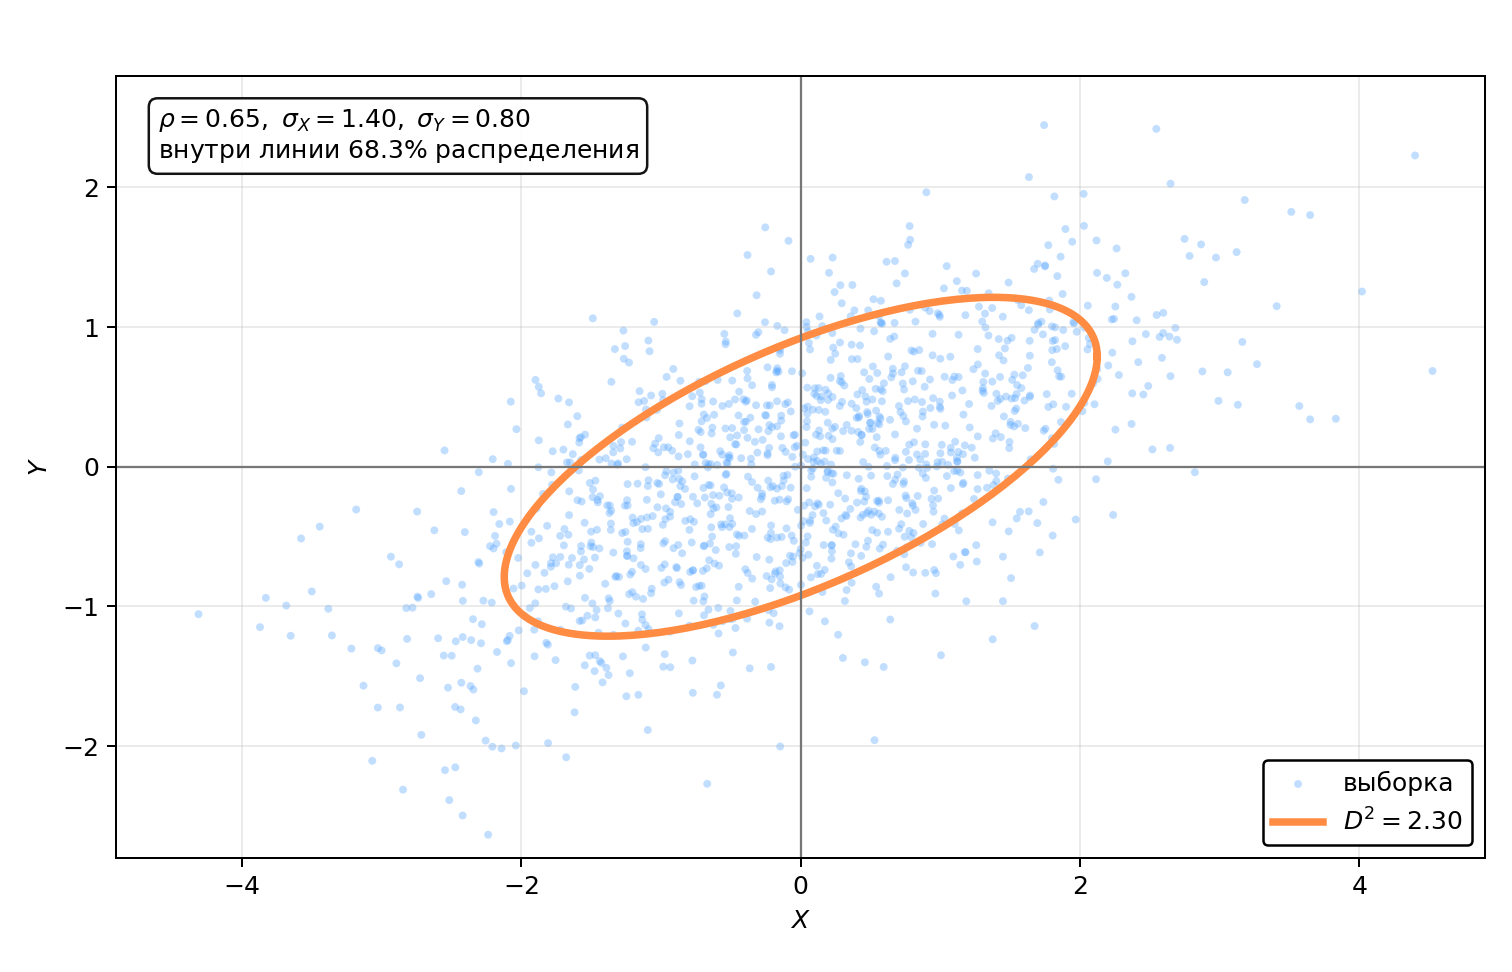
\includegraphics[width=0.74\linewidth,height=\textheight,keepaspectratio,alt={корреляция и эллипс}]{assets/figures/gaussian2d_correlation_ellipse.png}

\end{center}

\noindent\begin{minipage}[c]{\dimexpr\linewidth-30mm\relax}

\textbf{Интерактив}. \textbf{корреляция и эллипс}

Меняйте \(\rho\), \(\sigma_X\) и \(\sigma_Y\). Точки показывают выборку
из двумерного гаусса, линия --- эллипс \(D^2=2.30\).

\end{minipage}\hfill\begin{minipage}[c]{26mm}\centering

\href{https://neutrinohit.github.io/statistical-analysis-course/ru/book/chapters/07_two_dimensional_gaussian.html\#interactive-gaussian-correlation-ellipse}{
\includegraphics[width=24mm,height=\textheight,keepaspectratio,alt={QR-код интерактива}]{assets/qr/gaussian-correlation-ellipse.png}}

\end{minipage}

\end{semanticpdfbox}

При изменении \(\rho\) меняются сразу направление и длины осей. Матрица
с теми же диагональными элементами, но другой ковариацией задаёт другое
совместное распределение.

\section{Сколько вероятности находится внутри
эллипса}\label{ux441ux43aux43eux43bux44cux43aux43e-ux432ux435ux440ux43eux44fux442ux43dux43eux441ux442ux438-ux43dux430ux445ux43eux434ux438ux442ux441ux44f-ux432ux43dux443ux442ux440ux438-ux44dux43bux43bux438ux43fux441ux430}

В одном измерении фраза «в пределах одной сигмы» понятна:

\begin{equation}\protect\phantomsection\label{eq-ch7-one-dimensional-one-sigma}{
P(|Z|\leq1)=0.683,
\qquad Z\sim\mathcal N(0,1).
}\end{equation}

После появления второй оси требуется уточнить область. Для двумерного
гаусса стандартизованные координаты независимы, поэтому

\begin{equation}\protect\phantomsection\label{eq-ch7-mahalanobis-chi-square-two}{
D^2=Z_1^2+Z_2^2\sim\chi_2^2.
}\end{equation}

Плотность \(\chi_2^2\) особенно проста:

\begin{equation}\protect\phantomsection\label{eq-ch7-chi-square-two-density}{
f_{\chi_2^2}(q)=\frac12e^{-q/2},
\qquad q\geq0.
}\end{equation}

Интегрируя её от нуля до \(c\), получаем вероятность внутри эллипса:

\begin{equation}\protect\phantomsection\label{eq-ch7-contour-probability}{
P(D^2\leq c)=1-e^{-c/2}.
}\end{equation}

Для заданной вероятности \(P\) граница находится из обратной формулы

\begin{equation}\protect\phantomsection\label{eq-ch7-contour-threshold}{
c=-2\ln(1-P).
}\end{equation}

Значение \(c=1\) в двух измерениях даёт

\begin{equation}\protect\phantomsection\label{eq-ch7-two-dimensional-unit-contour}{
P(D^2\leq1)=1-e^{-1/2}=0.393.
}\end{equation}

В таблице \ref{tbl-ch7-contour-probabilities} приведены уровни, которые
часто встречаются на двумерных графиках.

\begin{longtable}[]{@{}rr@{}}
\caption{Вероятностные уровни двумерного гауссова
распределения}\label{tbl-ch7-contour-probabilities}\tabularnewline
\toprule\noalign{}
Вероятность внутри контура & Граница \(c\) \\
\midrule\noalign{}
\endfirsthead
\toprule\noalign{}
Вероятность внутри контура & Граница \(c\) \\
\midrule\noalign{}
\endhead
\bottomrule\noalign{}
\endlastfoot
\(39.3\%\) & \(1.00\) \\
\(68.3\%\) & \(2.30\) \\
\(90\%\) & \(4.61\) \\
\(95\%\) & \(5.99\) \\
\(99\%\) & \(9.21\) \\
\end{longtable}

\subsection{Интерактив: вероятность и размер
контура}\label{interactive-gaussian-probability-contour}

\begin{semanticpdfbox}[breakable=false]

\begin{center}

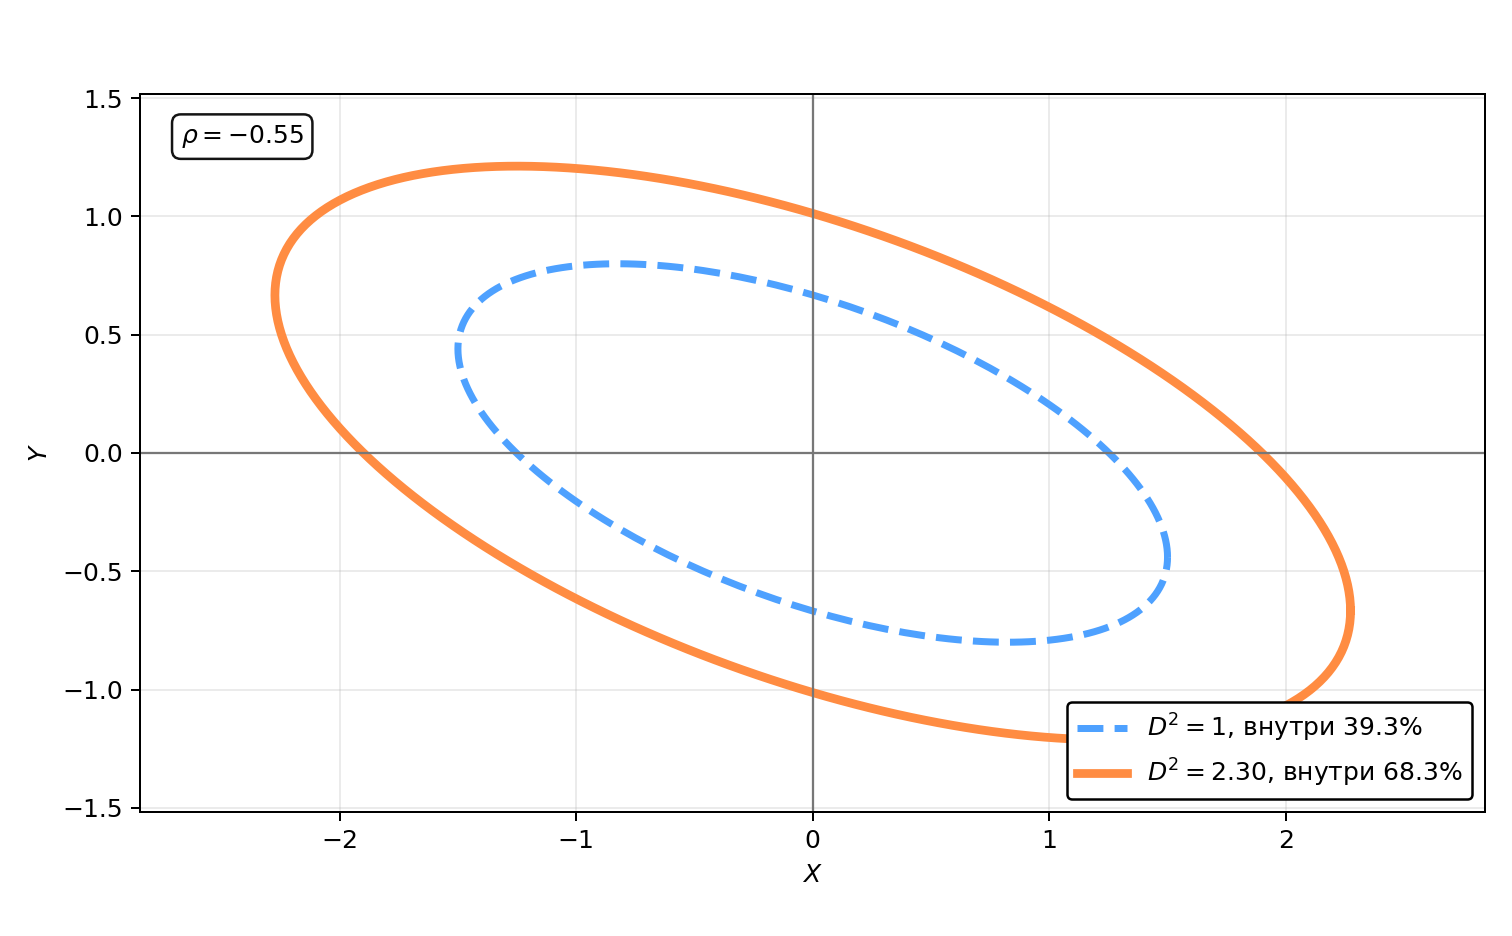
\includegraphics[width=0.74\linewidth,height=\textheight,keepaspectratio,alt={вероятность и размер контура}]{assets/figures/gaussian2d_probability_contour.png}

\end{center}

\noindent\begin{minipage}[c]{\dimexpr\linewidth-30mm\relax}

\textbf{Интерактив}. \textbf{вероятность и размер контура}

Сплошная линия ограничивает выбранную долю распределения. Пунктир
показывает \(D^2=1\), который в двух измерениях содержит \(39.3\%\)
вероятности.

\end{minipage}\hfill\begin{minipage}[c]{26mm}\centering

\href{https://neutrinohit.github.io/statistical-analysis-course/ru/book/chapters/07_two_dimensional_gaussian.html\#interactive-gaussian-probability-contour}{
\includegraphics[width=24mm,height=\textheight,keepaspectratio,alt={QR-код интерактива}]{assets/qr/gaussian-probability-contour.png}}

\end{minipage}

\end{semanticpdfbox}

\subsection{Возвращение к
калориметру}\label{ux432ux43eux437ux432ux440ux430ux449ux435ux43dux438ux435-ux43a-ux43aux430ux43bux43eux440ux438ux43cux435ux442ux440ux443}

Для измерения \ref{eq-ch7-calorimeter-measurement} мы нашли
\(D^2=1.54\). Уравнение \ref{eq-ch7-contour-probability} даёт

\begin{equation}\protect\phantomsection\label{eq-ch7-calorimeter-contained-probability}{
P(D^2\leq1.54)=1-e^{-1.54/2}=0.537.
}\end{equation}

Иными словами, эллипс через эту точку содержит около \(54\%\)
распределения. Точка лежит внутри области \(68.3\%\), поскольку
\(1.54<2.30\). Положительная корреляция здесь существенна: оба измерения
отклонились в одну сторону, то есть вдоль вытянутой оси облака.

\subsection{Распределение данных и пространство
параметров}\label{ux440ux430ux441ux43fux440ux435ux434ux435ux43bux435ux43dux438ux435-ux434ux430ux43dux43dux44bux445-ux438-ux43fux440ux43eux441ux442ux440ux430ux43dux441ux442ux432ux43e-ux43fux430ux440ux430ux43cux435ux442ux440ux43eux432}

Эллипсы этой главы описывают случайный вектор \(\mathbf X\) при
известных \(\boldsymbol\mu\) и \(V\). В статьях похожие контуры часто
рисуют в пространстве оцениваемых параметров вокруг полученного
минимума. Одинаковая квадратичная форма ещё не делает их одним объектом.

Для параметров вероятностная интерпретация зависит от того, как построен
интервал: от распределения оценки в частотном подходе или от
апостериорной плотности в байесовском. Значения \(2.30\), \(4.61\) и
\(5.99\) применимы к двумерной квадратичной гауссовой задаче. Условия,
при которых ими можно пользоваться для параметров, мы обсудим вместе с
правдоподобием и \(\chi^2\).

\section{Объединение
измерений}\label{ux43eux431ux44aux435ux434ux438ux43dux435ux43dux438ux435-ux438ux437ux43cux435ux440ux435ux43dux438ux439}

Пусть \(n\) приборов измеряют одну величину \(\mu\). Результаты собраны
в вектор \(\mathbf x\), а их ковариационная матрица равна \(V\). Если
совместное распределение гауссово, значение \(\mu\), при котором
полученные данные имеют наибольшую плотность, минимизирует

\begin{equation}\protect\phantomsection\label{eq-ch7-combination-quadratic-form}{
Q(\mu)=
(\mathbf x-\mu\mathbf1)^{\mathsf T}
V^{-1}
(\mathbf x-\mu\mathbf1).
}\end{equation}

Здесь \(\mathbf1\) --- вектор из единиц. Дифференцирование по \(\mu\)
даёт

\begin{equation}\protect\phantomsection\label{eq-ch7-correlated-weighted-mean}{
\widehat\mu=
\frac{\mathbf1^{\mathsf T}V^{-1}\mathbf x}
{\mathbf1^{\mathsf T}V^{-1}\mathbf1},
\qquad
\operatorname{Var}(\widehat\mu)=
\frac{1}{\mathbf1^{\mathsf T}V^{-1}\mathbf1}.
}\end{equation}

Это несмещённая линейная комбинация с наименьшей дисперсией. При
независимых измерениях \(V\) диагональна, и формула принимает знакомый
вид

\begin{equation}\protect\phantomsection\label{eq-ch7-independent-weighted-mean}{
\widehat\mu=
\frac{\displaystyle\sum_{i=1}^{n}x_i/\sigma_i^2}
{\displaystyle\sum_{i=1}^{n}1/\sigma_i^2},
\qquad
\operatorname{Var}(\widehat\mu)=
\frac{1}{\displaystyle\sum_{i=1}^{n}1/\sigma_i^2}.
}\end{equation}

Для двух измерений с ковариацией \(c_{12}\) веса можно выписать явно:

\begin{equation}\protect\phantomsection\label{eq-ch7-two-measurement-weights}{
\widehat\mu=w_1x_1+w_2x_2,
\qquad
w_1=\frac{\sigma_2^2-c_{12}}
{\sigma_1^2+\sigma_2^2-2c_{12}},
\qquad
w_2=\frac{\sigma_1^2-c_{12}}
{\sigma_1^2+\sigma_2^2-2c_{12}}.
}\end{equation}

Сумма весов равна единице. Один из них может оказаться отрицательным,
если корреляция велика, а точности измерений заметно различаются.
Отрицательный вес помогает оценить общую флуктуацию по второму измерению
и частично вычесть её из более точного результата.

\section{Инвариантная масса двух
частиц}\label{ux438ux43dux432ux430ux440ux438ux430ux43dux442ux43dux430ux44f-ux43cux430ux441ux441ux430-ux434ux432ux443ux445-ux447ux430ux441ux442ux438ux446}

Возьмём ещё один пример из лекции. Для двух безмассовых частиц с
энергиями \(E_1\), \(E_2\) и углом \(\theta\) между импульсами

\begin{equation}\protect\phantomsection\label{eq-ch7-invariant-mass}{
m^2=2E_1E_2(1-\cos\theta).
}\end{equation}

Вектор измеряемых величин и его ковариационная матрица равны

\begin{equation}\protect\phantomsection\label{eq-ch7-invariant-mass-input-covariance}{
\mathbf x=
\begin{pmatrix}
E_1\\
E_2\\
\theta
\end{pmatrix},
\qquad
V_{\mathbf x}=
\begin{pmatrix}
1.44 & 0.36 & 0\\
0.36 & 1.00 & 0\\
0 & 0 & 2.5\cdot10^{-5}
\end{pmatrix}.
}\end{equation}

В энергетическом блоке числа указаны в \(\text{ГэВ}^2\), угловая
дисперсия --- в \(\text{рад}^2\). Возьмём

\begin{equation}\protect\phantomsection\label{eq-ch7-invariant-mass-input-values}{
E_1=60.0\ \text{ГэВ},
\qquad
E_2=40.0\ \text{ГэВ},
\qquad
\theta=0.200\ \text{рад}.
}\end{equation}

Градиент квадрата массы равен

\begin{equation}\protect\phantomsection\label{eq-ch7-invariant-mass-gradient}{
\nabla m^2=
\begin{pmatrix}
2E_2(1-\cos\theta)\\
2E_1(1-\cos\theta)\\
2E_1E_2\sin\theta
\end{pmatrix}.
}\end{equation}

\begin{bookderivation}

\subsubsection{Численный
расчёт}\label{ux447ux438ux441ux43bux435ux43dux43dux44bux439-ux440ux430ux441ux447ux451ux442}

Сначала найдём саму массу:

\begin{equation}\protect\phantomsection\label{eq-ch7-invariant-mass-value}{
m^2=2\cdot60\cdot40(1-\cos0.200)
=95.680\ \text{ГэВ}^2,
\qquad
m=9.782\ \text{ГэВ}.
}\end{equation}

В заданной точке численный градиент равен

\begin{equation}\protect\phantomsection\label{eq-ch7-invariant-mass-gradient-numeric}{
\nabla m^2=
\begin{pmatrix}
1.595\\
2.392\\
953.613
\end{pmatrix}.
}\end{equation}

По формуле распространения ковариации из главы 6

\begin{equation}\protect\phantomsection\label{eq-ch7-invariant-mass-variance}{
\operatorname{Var}(m^2)
\simeq
(\nabla m^2)^{\mathsf T}
V_{\mathbf x}
(\nabla m^2)
=34.864\ \text{ГэВ}^4.
}\end{equation}

Отсюда

\begin{equation}\protect\phantomsection\label{eq-ch7-invariant-mass-uncertainties}{
\sigma_{m^2}=5.905\ \text{ГэВ}^2,
\qquad
\sigma_m\simeq\frac{\sigma_{m^2}}{2m}
=0.302\ \text{ГэВ}.
}\end{equation}

Результат можно записать как

\begin{equation}\protect\phantomsection\label{eq-ch7-invariant-mass-result}{
m=(9.78\pm0.30)\ \text{ГэВ}.
}\end{equation}

\end{bookderivation}

Ковариация двух энергий даёт в дисперсию \(m^2\) вклад

\begin{equation}\protect\phantomsection\label{eq-ch7-invariant-mass-correlation-contribution}{
2\frac{\partial m^2}{\partial E_1}
\frac{\partial m^2}{\partial E_2}
\operatorname{cov}(E_1,E_2)
=2.75\ \text{ГэВ}^4.
}\end{equation}

Если этот член отбросить, получится \(\sigma_m=0.290\) ГэВ вместо
\(0.302\) ГэВ. Та же положительная корреляция, которая наклоняла эллипс
двух энергий, увеличивает ошибку массы: обе производные по энергиям
положительны.

\section{Где заканчивается гауссова
геометрия}\label{ux433ux434ux435-ux437ux430ux43aux430ux43dux447ux438ux432ux430ux435ux442ux441ux44f-ux433ux430ux443ux441ux441ux43eux432ux430-ux433ux435ux43eux43cux435ux442ux440ux438ux44f}

Многомерный гаусс полностью определяется средним и ковариационной
матрицей. Для произвольного распределения этих двух объектов уже
недостаточно. Два распределения могут иметь одинаковые
\(\boldsymbol\mu\) и \(V\), но разные хвосты и разную вероятность
далёких отклонений.

Линейное распространение ковариации хорошо описывает малые флуктуации
около рабочей точки. Сильная нелинейность, асимметричные входные
распределения и физические границы требуют распространения полного
распределения. Один из способов сделать это --- сгенерировать входные
величины с заданными связями и пропустить их через функцию результата.

Отдельная численная трудность возникает при \(|\rho|\simeq1\). Матрица
\(V\) становится почти вырожденной, и результат обращения чувствителен к
малым изменениям её элементов. Это означает, что два измерения содержат
почти одну и ту же информацию. Печатать больше знаков в \(V^{-1}\) здесь
бесполезно: следует проверить модель общей ошибки.

\begin{bookchaptersummary}[Итоги главы]

\begin{itemize}
\tightlist
\item
  Ковариационная матрица задаёт масштабы и направления флуктуаций
  многомерного гаусса.
\item
  Квадрат расстояния Махаланобиса учитывает единицы, дисперсии и
  корреляции.
\item
  В двух измерениях область \(D^2\leq1\) содержит \(39.3\%\)
  вероятности; для \(68.3\%\) нужна граница \(D^2=2.30\).
\item
  Объединение измерений и распространение ошибок требуют полной
  ковариационной матрицы.
\end{itemize}

\end{bookchaptersummary}

\section{Задачи}\label{ux437ux430ux434ux430ux447ux438-6}

\begin{semanticpdfbox}[colback=BookCoralSoft,borderline west={1.2mm}{0pt}{BookCoral},breakable=false]

\noindent{\sffamily\bfseries\fontsize{11.2}{13.5}\selectfont Задача 1. Вероятность внутри эллипса}\par\nopagebreak[4]\vspace{1.2mm}

Для двумерного гауссова распределения

\[
D^2=(\mathbf X-\boldsymbol\mu)^{\mathsf T}
V^{-1}(\mathbf X-\boldsymbol\mu)
\sim\chi_2^2.
\]

\begin{enumerate}
\def\labelenumi{\arabic{enumi}.}
\tightlist
\item
  Получите плотность \(D^2\) и покажите, что \[
  P(D^2\leq c)=1-e^{-c/2}.
  \]
\item
  Найдите \(c\) для областей с вероятностями \(68.3\%\), \(90\%\) и
  \(95\%\).
\item
  Вычислите вероятность внутри контура \(D^2=1\).
\item
  Сравните этот результат с одномерной вероятностью \(P(|Z|\leq1)\) и
  объясните различие.
\end{enumerate}

\end{semanticpdfbox}

\begin{semanticpdfbox}[colback=BookCoralSoft,borderline west={1.2mm}{0pt}{BookCoral},breakable=false]

\noindent{\sffamily\bfseries\fontsize{11.2}{13.5}\selectfont Задача 2. Геометрия ковариационной матрицы}\par\nopagebreak[4]\vspace{1.2mm}

Даны средний вектор и ковариационная матрица двух измеренных энергий:

\[
\boldsymbol\mu=
\begin{pmatrix}60\\40\end{pmatrix}\ \text{ГэВ},
\qquad
V=
\begin{pmatrix}
1.44&0.36\\
0.36&1.00
\end{pmatrix}\ \text{ГэВ}^2.
\]

\begin{enumerate}
\def\labelenumi{\arabic{enumi}.}
\tightlist
\item
  Найдите стандартные отклонения и коэффициент корреляции.
\item
  Вычислите собственные значения и собственные векторы \(V\).
\item
  Найдите длины и направления полуосей эллипса \(D^2=2.30\).
\item
  Для точки \(\mathbf x=(61.2,41.0)^{\mathsf T}\) ГэВ вычислите \(D^2\)
  и определите, лежит ли она внутри области с вероятностью \(68.3\%\).
\end{enumerate}

\end{semanticpdfbox}

\begin{semanticpdfbox}[colback=BookCoralSoft,borderline west={1.2mm}{0pt}{BookCoral},breakable=false]

\noindent{\sffamily\bfseries\fontsize{11.2}{13.5}\selectfont Задача 3. Объединение двух измерений}\par\nopagebreak[4]\vspace{1.2mm}

Одна величина измерена двумя способами:

\[
x_1=10.2\pm0.8,
\qquad
x_2=11.1\pm0.4.
\]

\begin{enumerate}
\def\labelenumi{\arabic{enumi}.}
\tightlist
\item
  Найдите взвешенное среднее и его стандартное отклонение, считая
  измерения независимыми.
\item
  Повторите расчёт для коэффициента корреляции \(\rho=0.6\).
\item
  Выпишите оба веса во втором случае и объясните знак каждого из них.
\item
  Проверьте, что ковариационная матрица положительно определена.
\end{enumerate}

\end{semanticpdfbox}

\begin{semanticpdfbox}[colback=BookCoralSoft,borderline west={1.2mm}{0pt}{BookCoral},breakable=false]

\noindent{\sffamily\bfseries\fontsize{11.2}{13.5}\selectfont Задача 4. Инвариантная масса}\par\nopagebreak[4]\vspace{1.2mm}

Для двух безмассовых частиц

\[
m^2=2E_1E_2(1-\cos\theta).
\]

Пусть \(E_1=60\) ГэВ, \(E_2=40\) ГэВ, \(\theta=0.200\) рад, а
ковариационная матрица величин \((E_1,E_2,\theta)\) равна

\[
V=
\begin{pmatrix}
1.44&0.36&0\\
0.36&1.00&0\\
0&0&2.5\cdot10^{-5}
\end{pmatrix}.
\]

\begin{enumerate}
\def\labelenumi{\arabic{enumi}.}
\tightlist
\item
  Найдите градиент \(m^2\) и вычислите \(\sigma_{m^2}\).
\item
  Получите \(\sigma_m\) линейным распространением ошибки.
\item
  Повторите расчёт при \(\operatorname{cov}(E_1,E_2)=0\) и сравните
  ответы.
\item
  Исследуйте предел \(\theta\ll1\): получите приближённые выражения для
  \(m\) и его производных.
\end{enumerate}

\end{semanticpdfbox}

\section*{Литература}\label{ux43bux438ux442ux435ux440ux430ux442ux443ux440ux430-6}
\addcontentsline{toc}{section}{Литература}

\markright{Литература}

\protect\phantomsection\label{refs}
\begin{CSLReferences}{0}{0}
\bibitem[\citeproctext]{ref-cowan1998}
{[}1{]} Cowan, G. \emph{Statistical Data Analysis}. Oxford University
Press. 1998.

\end{CSLReferences}

\chapter{Метод Монте-Карло и
псевдоэксперименты}\label{ux43cux435ux442ux43eux434-ux43cux43eux43dux442ux435-ux43aux430ux440ux43bux43e-ux438-ux43fux441ux435ux432ux434ux43eux44dux43aux441ux43fux435ux440ux438ux43cux435ux43dux442ux44b}

\bookchapteropeningcontents

\begin{bookchapteropening}[Аннотация]

Метод Монте-Карло позволяет заменить сложный расчёт большим числом
случайных реализаций заданной модели. В этой главе мы разберём генерацию
случайных величин, вычисление многомерных интегралов, выборку по
важности и алгоритм VEGAS. Затем построим ансамбль псевдоэкспериментов и
проследим цепочку от генерации физического процесса до отклика детектора
и результата анализа.

\end{bookchapteropening}

\section{Физическая задача: слабый сигнал на
фоне}\label{ux444ux438ux437ux438ux447ux435ux441ux43aux430ux44f-ux437ux430ux434ux430ux447ux430-ux441ux43bux430ux431ux44bux439-ux441ux438ux433ux43dux430ux43b-ux43dux430-ux444ux43eux43dux435}

Эксперимент ищет редкий процесс. За время набора данных ожидается в
среднем \(s=5\) сигнальных и \(b=10\) фоновых событий. Полное число
зарегистрированных событий имеет распределение Пуассона:

\begin{equation}\protect\phantomsection\label{eq-ch8-counting-model}{
N\sim\operatorname{Pois}(s+b).
}\end{equation}

Будем считать фон известным точно и оценим число сигнальных событий
простым вычитанием:

\begin{equation}\protect\phantomsection\label{eq-ch8-counting-estimator}{
\widehat s=N-b.
}\end{equation}

До проведения эксперимента можно задать несколько вполне физических
вопросов. Какое значение \(\widehat s\) мы в среднем получим? Каков
разброс оценки? Как часто флуктуация фона приведёт к отрицательному
\(\widehat s\)?

Первые два ответа следуют из свойств распределения Пуассона:

\begin{equation}\protect\phantomsection\label{eq-ch8-counting-moments}{
\mathbb E[\widehat s]=s,
\qquad
\operatorname{Var}(\widehat s)=s+b.
}\end{equation}

Для \(s=5\) и \(b=10\) стандартное отклонение равно
\(\sqrt{15}\simeq3.87\) события. Отрицательная оценка получается при
\(N<10\). Её вероятность равна

\begin{equation}\protect\phantomsection\label{eq-ch8-negative-signal-probability}{
P(\widehat s<0)
=P(N\leq9\mid s+b=15)
=\sum_{n=0}^{9}e^{-15}\frac{15^n}{n!}
=0.0699.
}\end{equation}

Эту задачу можно решить и численно. Сгенерируем много значений
\(N_k\sim\operatorname{Pois}(15)\), для каждого вычислим
\(\widehat s_k=N_k-10\) и посмотрим на полученное распределение. Его
среднее, дисперсия и доля отрицательных оценок приблизятся к значениям в
формулах \ref{eq-ch8-counting-moments} и
\ref{eq-ch8-negative-signal-probability}.

В этой игрушечной модели аналитический ответ помещается в несколько
строк. Настоящий анализ использует энергетический спектр, отклик
детектора, отбор событий и мешающие параметры. Распределение результата
такой процедуры обычно уже нельзя выписать одной формулой. Тогда мы
повторяем эксперимент на компьютере. Это и есть метод Монте-Карло.

\section{Что вычисляет метод
Монте-Карло}\label{ux447ux442ux43e-ux432ux44bux447ux438ux441ux43bux44fux435ux442-ux43cux435ux442ux43eux434-ux43cux43eux43dux442ux435-ux43aux430ux440ux43bux43e}

Пусть случайная величина \(X\) имеет плотность \(f_X(x)\), а
интересующая нас величина определяется функцией \(g\):

\begin{equation}\protect\phantomsection\label{eq-ch8-general-transformation}{
X\sim f_X(x),
\qquad
Y=g(X).
}\end{equation}

Численный алгоритм состоит из трёх действий:

\begin{enumerate}
\def\labelenumi{\arabic{enumi}.}
\tightlist
\item
  сгенерировать независимые значения \(X_1,\ldots,X_N\) из распределения
  \(f_X\);
\item
  вычислить \(Y_k=g(X_k)\) для каждого события;
\item
  по выборке \(Y_1,\ldots,Y_N\) найти среднее, дисперсию, вероятность
  нужного события или всё распределение \(Y\).
\end{enumerate}

В короткой записи

\begin{equation}\protect\phantomsection\label{eq-ch8-monte-carlo-sample}{
X_k\sim f_X,
\qquad
Y_k=g(X_k),
\qquad
k=1,\ldots,N.
}\end{equation}

Один и тот же принцип используется в нескольких задачах. Интеграл можно
записать как математическое ожидание,

\begin{equation}\protect\phantomsection\label{eq-ch8-integral-as-expectation}{
\int h(x)f_X(x)\,dx=\mathbb E[h(X)].
}\end{equation}

При распространении ошибок генерируется случайный вектор \(\mathbf X\),
после чего для каждого события вычисляется \(Y=g(\mathbf X)\).
Псевдоэксперимент воспроизводит весь анализ целиком.

Метод был сформулирован как общий численный подход Метрополисом и Уламом
в 1949 году {[}1{]}. Его точность определяется числом реализаций и
дисперсией вычисляемой величины.

\begin{booknote}

Монте-Карло решает задачу, записанную в программе. Если в модели нет
важного фона или неверно описан отклик детектора, увеличение числа
событий закрепит неверный ответ с меньшей численной ошибкой. Компьютер в
этом смысле безупречно послушен.

\end{booknote}

\section{Псевдослучайные
числа}\label{ux43fux441ux435ux432ux434ux43eux441ux43bux443ux447ux430ux439ux43dux44bux435-ux447ux438ux441ux43bux430}

Генератор псевдослучайных чисел мы уже использовали при обсуждении
центральной предельной теоремы. Это детерминированный алгоритм. Его
внутреннее состояние определяет всю дальнейшую последовательность

\begin{equation}\protect\phantomsection\label{eq-ch8-uniform-pseudorandom-sequence}{
U_1,U_2,\ldots,
\qquad
U_k\in[0,1),
}\end{equation}

которая проходит статистические тесты как выборка из равномерного
распределения. Период хорошего генератора намного превышает длину
обычного расчёта.

Начальное состояние задаётся начальным числом, или \emph{seed}.
Одинаковое начальное число воспроизводит ту же последовательность. Это
позволяет повторить расчёт и найти событие, на котором сломалась
программа.

Для параллельной генерации нужны независимые последовательности. Если
тысячу процессов запустить с одним начальным состоянием, каждый из них
создаст одну и ту же тысячу событий. В файле окажется миллион строк, а
независимых событий останется тысяча. Поэтому вместе с конфигурацией
анализа сохраняют алгоритм генератора и правило формирования начальных
состояний.

Большинство генераторов непосредственно создаёт

\begin{equation}\protect\phantomsection\label{eq-ch8-base-uniform-distribution}{
U\sim\mathrm U(0,1).
}\end{equation}

Из равномерной величины можно получить другие распределения.

\section{Метод обратной функции
распределения}\label{ux43cux435ux442ux43eux434-ux43eux431ux440ux430ux442ux43dux43eux439-ux444ux443ux43dux43aux446ux438ux438-ux440ux430ux441ux43fux440ux435ux434ux435ux43bux435ux43dux438ux44f}

Пусть \(F_X(x)\) --- функция распределения требуемой величины:

\begin{equation}\protect\phantomsection\label{eq-ch8-cumulative-distribution}{
F_X(x)=P(X\leq x)
=\int_{-\infty}^{x}f_X(t)\,dt.
}\end{equation}

Она монотонно возрастает от нуля до единицы. Если обратную функцию можно
вычислить, берём \(U\sim\mathrm U(0,1)\) и полагаем

\begin{equation}\protect\phantomsection\label{eq-ch8-inverse-transform-sampling}{
\boxed{X=F_X^{-1}(U).}
}\end{equation}

\begin{bookderivation}

\subsubsection{Почему это
работает}\label{ux43fux43eux447ux435ux43cux443-ux44dux442ux43e-ux440ux430ux431ux43eux442ux430ux435ux442}

Монотонность \(F_X\) даёт

\begin{equation}\protect\phantomsection\label{eq-ch8-inverse-transform-proof}{
\begin{aligned}
P(X\leq x)
&=P\!\left(F_X^{-1}(U)\leq x\right)\\
&=P\!\left(U\leq F_X(x)\right)\\
&=F_X(x).
\end{aligned}
}\end{equation}

В последней строке использовано \(P(U\leq u)=u\) для равномерной
величины на \([0,1]\). Получена требуемая функция распределения.
\(\blacksquare\)

\end{bookderivation}

\subsection{Пример: время между
событиями}\label{ux43fux440ux438ux43cux435ux440-ux432ux440ux435ux43cux44f-ux43cux435ux436ux434ux443-ux441ux43eux431ux44bux442ux438ux44fux43cux438}

Пусть события образуют пуассоновский процесс с интенсивностью
\(\lambda\). Время \(X\) до следующего события имеет экспоненциальную
плотность

\begin{equation}\protect\phantomsection\label{eq-ch8-exponential-density}{
f_X(x)=\lambda e^{-\lambda x},
\qquad x\geq0,
}\end{equation}

и функцию распределения

\begin{equation}\protect\phantomsection\label{eq-ch8-exponential-cdf}{
F_X(x)=1-e^{-\lambda x}.
}\end{equation}

Решая уравнение \(U=F_X(X)\) относительно \(X\), получаем

\begin{equation}\protect\phantomsection\label{eq-ch8-exponential-inverse-transform}{
X=-\frac{1}{\lambda}\ln(1-U).
}\end{equation}

Величина \(1-U\) также равномерна на \([0,1]\), поэтому в программе
часто пишут

\begin{equation}\protect\phantomsection\label{eq-ch8-exponential-generator}{
\boxed{X=-\frac{1}{\lambda}\ln U.}
}\end{equation}

\section{Метод
отбора}\label{ux43cux435ux442ux43eux434-ux43eux442ux431ux43eux440ux430}

Обратную функцию удаётся найти не для каждого распределения. Пусть
плотность \(f(x)\) ограничена сверху другой плотностью \(g(x)\):

\begin{equation}\protect\phantomsection\label{eq-ch8-rejection-envelope}{
f(x)\leq M g(x),
}\end{equation}

причём из \(g(x)\) генерировать удобно. Алгоритм отбора устроен так:

\begin{enumerate}
\def\labelenumi{\arabic{enumi}.}
\tightlist
\item
  сгенерировать кандидата \(X\sim g(x)\);
\item
  независимо сгенерировать \(U\sim\mathrm U(0,1)\);
\item
  принять \(X\), если
  \begin{equation}\protect\phantomsection\label{eq-ch8-rejection-condition}{
  U\leq\frac{f(X)}{M g(X)};
  }\end{equation}
\item
  при невыполнении условия повторить попытку.
\end{enumerate}

Если обе плотности нормированы, средняя доля принятых событий равна
\(1/M\). Чем ближе оболочка \(Mg(x)\) к \(f(x)\), тем меньше вычислений
заканчивается отказом.

\subsection{\texorpdfstring{Пример: плотность
\(6x(1-x)\)}{Пример: плотность 6x(1-x)}}\label{interactive-monte-carlo-rejection-sampling}

Рассмотрим плотность

\begin{equation}\protect\phantomsection\label{eq-ch8-rejection-example-density}{
f(x)=6x(1-x),
\qquad 0\leq x\leq1.
}\end{equation}

Её максимум достигается при \(x=1/2\) и равен \(3/2\). Равномерно
генерируем точки в прямоугольнике \(0\leq x\leq1\), \(0\leq y\leq3/2\) и
принимаем точку, если \(y\leq f(x)\).

\begin{semanticpdfbox}[breakable=false]

\begin{center}

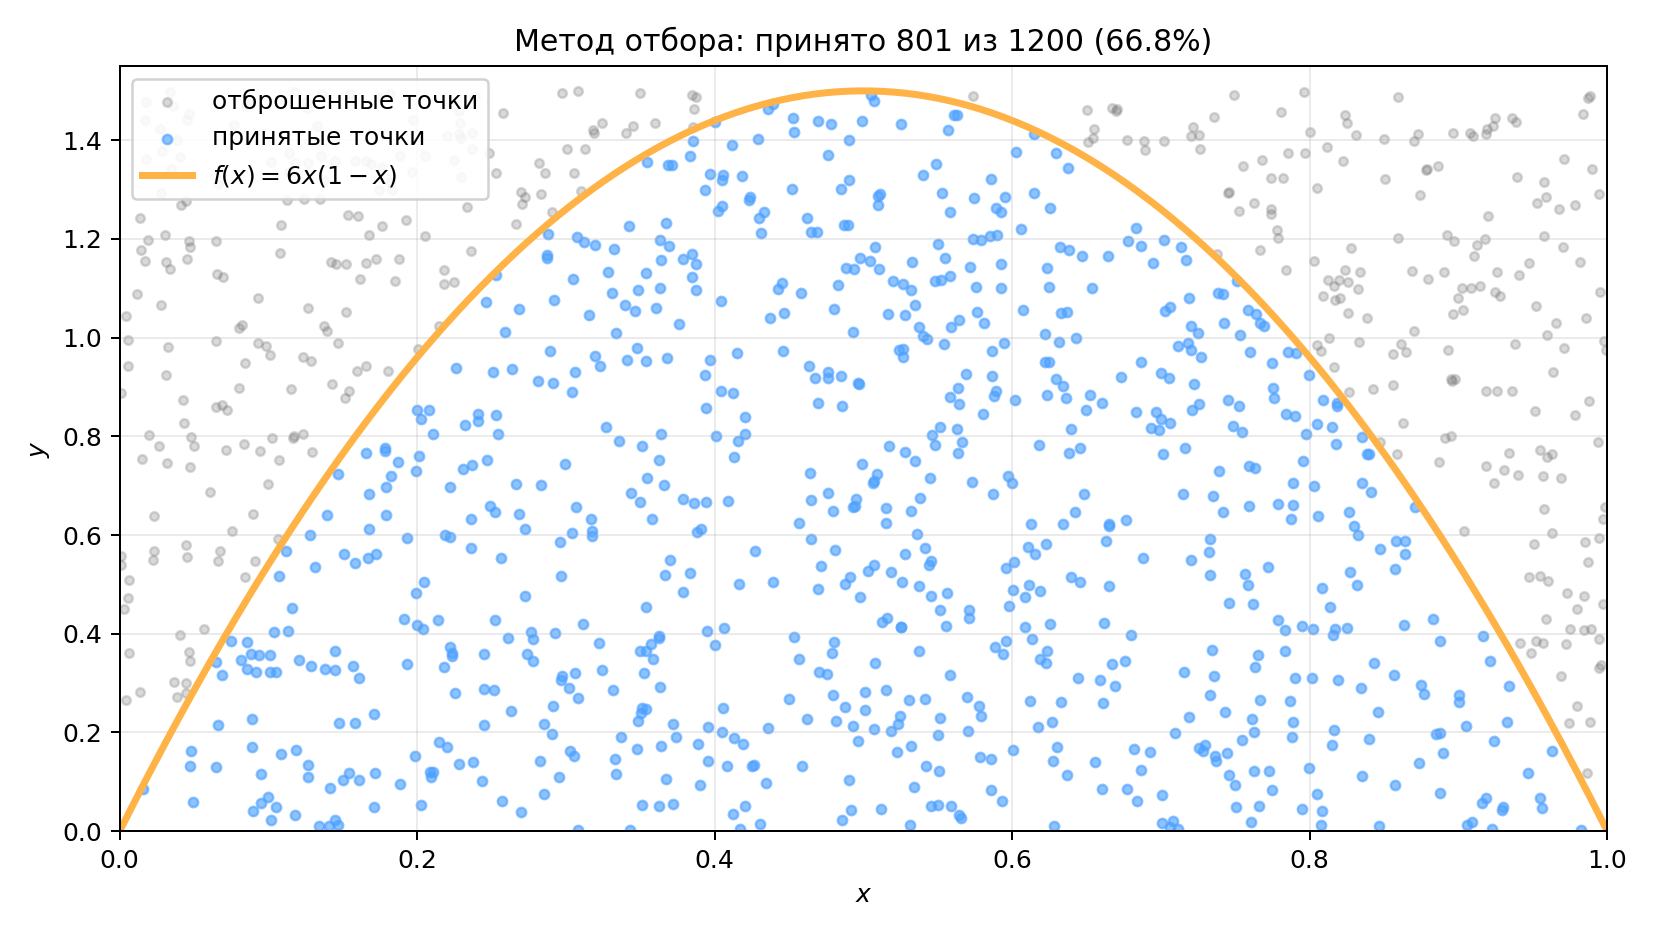
\includegraphics[width=0.74\linewidth,height=\textheight,keepaspectratio,alt={Метод отбора для плотности \$6x(1-x)\$}]{assets/figures/mc_rejection_sampling.png}

\end{center}

\noindent\begin{minipage}[c]{\dimexpr\linewidth-30mm\relax}

\textbf{Интерактив}. \textbf{Метод отбора для плотности \(6x(1-x)\)}

Синие точки приняты, серые отброшены. Теоретическая доля принятых
событий равна \(2/3\).

\end{minipage}\hfill\begin{minipage}[c]{26mm}\centering

\href{https://neutrinohit.github.io/statistical-analysis-course/ru/book/chapters/08_monte_carlo_method.html\#interactive-monte-carlo-rejection-sampling}{
\includegraphics[width=24mm,height=\textheight,keepaspectratio,alt={QR-код интерактива}]{assets/qr/monte-carlo-rejection-sampling.png}}

\end{minipage}

\end{semanticpdfbox}

\subsection{Как выбирать способ
генерации}\label{ux43aux430ux43a-ux432ux44bux431ux438ux440ux430ux442ux44c-ux441ux43fux43eux441ux43eux431-ux433ux435ux43dux435ux440ux430ux446ux438ux438}

\begin{longtable}[]{@{}
  >{\raggedright\arraybackslash}p{(\linewidth - 4\tabcolsep) * \real{0.3333}}
  >{\raggedright\arraybackslash}p{(\linewidth - 4\tabcolsep) * \real{0.3333}}
  >{\raggedright\arraybackslash}p{(\linewidth - 4\tabcolsep) * \real{0.3333}}@{}}
\caption{Основные способы генерации случайных
величин}\label{tbl-ch8-generation-methods}\tabularnewline
\toprule\noalign{}
\begin{minipage}[b]{\linewidth}\raggedright
Метод
\end{minipage} & \begin{minipage}[b]{\linewidth}\raggedright
Сильная сторона
\end{minipage} & \begin{minipage}[b]{\linewidth}\raggedright
Ограничение
\end{minipage} \\
\midrule\noalign{}
\endfirsthead
\toprule\noalign{}
\begin{minipage}[b]{\linewidth}\raggedright
Метод
\end{minipage} & \begin{minipage}[b]{\linewidth}\raggedright
Сильная сторона
\end{minipage} & \begin{minipage}[b]{\linewidth}\raggedright
Ограничение
\end{minipage} \\
\midrule\noalign{}
\endhead
\bottomrule\noalign{}
\endlastfoot
Обратная функция распределения & используется каждое сгенерированное
число & нужна вычислимая \(F_X^{-1}\) \\
Метод отбора & применим к широкому классу плотностей & плохая оболочка
снижает эффективность \\
Специальный алгоритм & может быть очень быстрым & нужна отдельная
реализация \\
Марковская цепь & работает со сложными многомерными плотностями &
значения коррелированы, сходимость требует проверки \\
\end{longtable}

\section{Интегрирование методом
Монте-Карло}\label{ux438ux43dux442ux435ux433ux440ux438ux440ux43eux432ux430ux43dux438ux435-ux43cux435ux442ux43eux434ux43eux43c-ux43cux43eux43dux442ux435-ux43aux430ux440ux43bux43e}

Рассмотрим одномерный интеграл

\begin{equation}\protect\phantomsection\label{eq-ch8-integral-definition}{
I=\int_a^b h(x)\,dx.
}\end{equation}

Если \(U\sim\mathrm U(a,b)\), то

\begin{equation}\protect\phantomsection\label{eq-ch8-uniform-integral-expectation}{
\mathbb E[h(U)]
=\frac{1}{b-a}\int_a^b h(x)\,dx.
}\end{equation}

Математическое ожидание заменим выборочным средним:

\begin{equation}\protect\phantomsection\label{eq-ch8-monte-carlo-integral-estimator}{
\boxed{
\widehat I_N
=\frac{b-a}{N}\sum_{k=1}^{N}h(U_k).
}
}\end{equation}

\subsection{Статистическая ошибка
интеграла}\label{ux441ux442ux430ux442ux438ux441ux442ux438ux447ux435ux441ux43aux430ux44f-ux43eux448ux438ux431ux43aux430-ux438ux43dux442ux435ux433ux440ux430ux43bux430}

\begin{bookderivation}

\subsubsection{\texorpdfstring{Дисперсия оценки
\(\widehat I_N\)}{Дисперсия оценки \textbackslash widehat I\_N}}\label{ux434ux438ux441ux43fux435ux440ux441ux438ux44f-ux43eux446ux435ux43dux43aux438-widehat-i_n}

Обозначим

\begin{equation}\protect\phantomsection\label{eq-ch8-integrand-variance}{
\operatorname{Var}[h(U)]=\sigma_h^2.
}\end{equation}

Для независимых точек дисперсии слагаемых складываются:

\begin{equation}\protect\phantomsection\label{eq-ch8-monte-carlo-integral-variance}{
\begin{aligned}
\operatorname{Var}(\widehat I_N)
&=\frac{(b-a)^2}{N^2}
  \operatorname{Var}\!\left(\sum_{k=1}^{N}h(U_k)\right)\\
&=\frac{(b-a)^2\sigma_h^2}{N}.
\end{aligned}
}\end{equation}

Следовательно,

\begin{equation}\protect\phantomsection\label{eq-ch8-monte-carlo-integral-error}{
\boxed{
\sigma_{\widehat I_N}
=\frac{(b-a)\sigma_h}{\sqrt N}.
}
}\end{equation}

\(\blacksquare\)

\end{bookderivation}

Чтобы уменьшить ошибку в десять раз, число точек придётся увеличить в
сто раз. Это медленная сходимость. Её важное достоинство проявляется в
большой размерности: показатель \(N^{-1/2}\) не превращается в
\(N^{-1/d}\). Коэффициент перед ним, конечно, зависит от конкретной
функции и выбранного распределения точек.

\section{\texorpdfstring{Проверка на числе
\(\pi\)}{Проверка на числе \textbackslash pi}}\label{interactive-monte-carlo-pi}

Равномерно сгенерируем точки в единичном квадрате:

\begin{equation}\protect\phantomsection\label{eq-ch8-pi-uniform-points}{
(X,Y)\sim\mathrm U([0,1]^2).
}\end{equation}

Точка лежит внутри четверти единичного круга при \(X^2+Y^2\leq1\).
Поэтому

\begin{equation}\protect\phantomsection\label{eq-ch8-quarter-circle-probability}{
P(X^2+Y^2\leq1)=\frac{\pi}{4},
}\end{equation}

и доля попавших внутрь точек даёт оценку

\begin{equation}\protect\phantomsection\label{eq-ch8-pi-estimator}{
\boxed{
\widehat\pi=4\frac{N_{\mathrm{in}}}{N}.
}
}\end{equation}

\begin{semanticpdfbox}[breakable=false]

\begin{center}

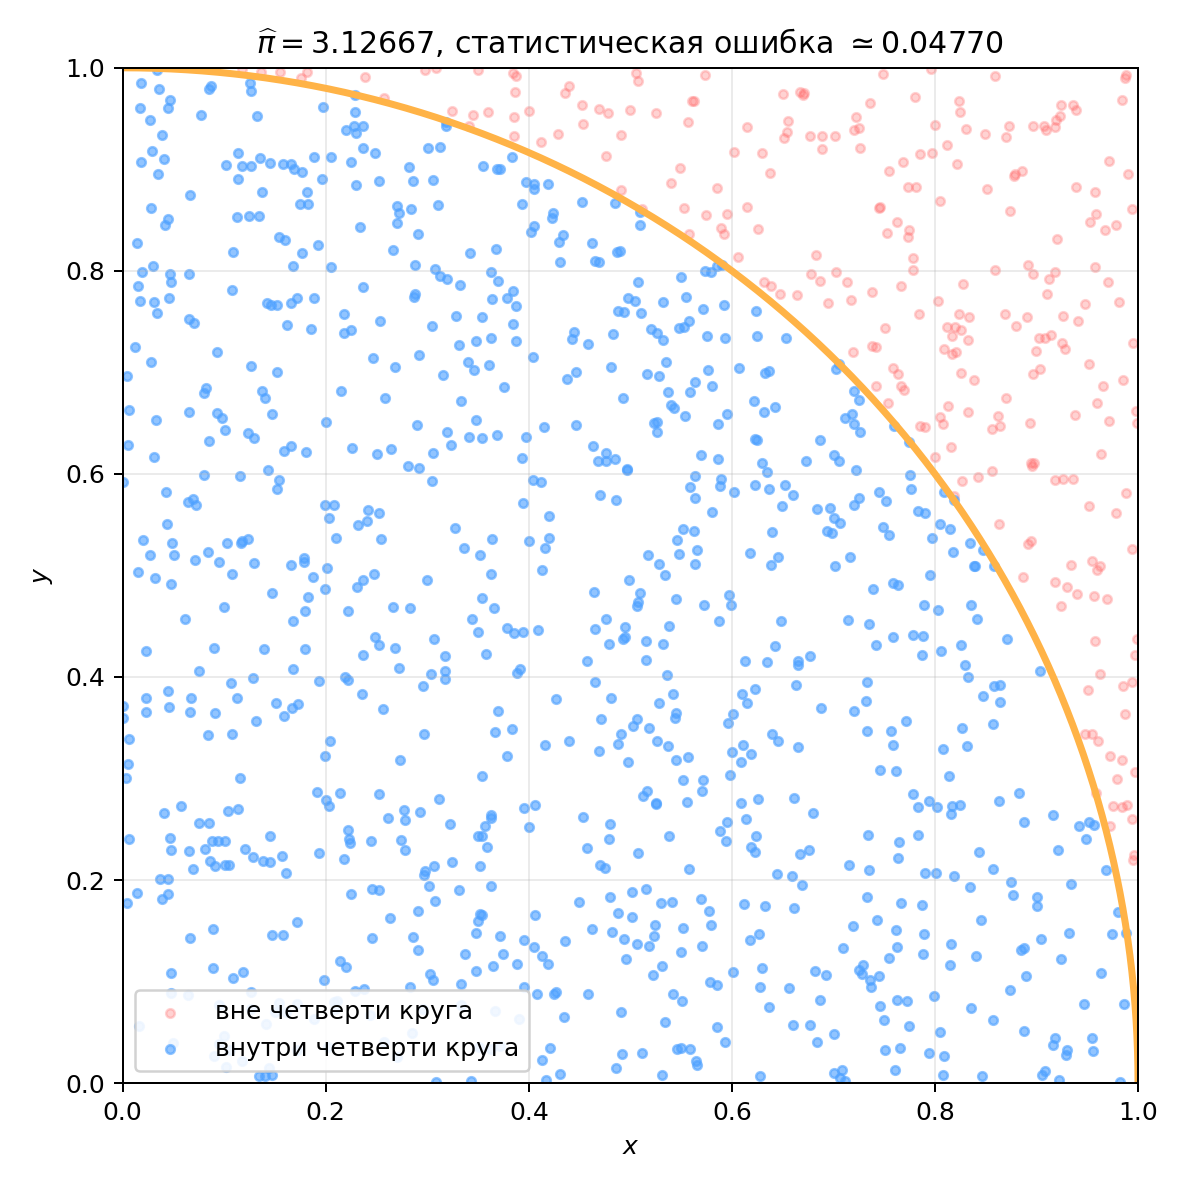
\includegraphics[width=0.74\linewidth,height=\textheight,keepaspectratio,alt={Оценка числа \$\textbackslash pi\$ методом Монте-Карло}]{assets/figures/mc_pi_estimate.png}

\end{center}

\noindent\begin{minipage}[c]{\dimexpr\linewidth-30mm\relax}

\textbf{Интерактив}. \textbf{Оценка числа \(\pi\) методом Монте-Карло}

Доля синих точек внутри четверти круга оценивает \(\pi/4\).

\end{minipage}\hfill\begin{minipage}[c]{26mm}\centering

\href{https://neutrinohit.github.io/statistical-analysis-course/ru/book/chapters/08_monte_carlo_method.html\#interactive-monte-carlo-pi}{
\includegraphics[width=24mm,height=\textheight,keepaspectratio,alt={QR-код интерактива}]{assets/qr/monte-carlo-pi.png}}

\end{minipage}

\end{semanticpdfbox}

Если единственная цель состоит в вычислении числа \(\pi\), калькулятор
справится лучше. Этот пример ценен другим: точный ответ известен,
геометрия видна на рисунке, а ошибка подчиняется закону \(1/\sqrt N\) из
формулы \ref{eq-ch8-monte-carlo-integral-error}. Такие задачи нужны для
проверки реализации метода.

\section{Высокая
размерность}\label{interactive-monte-carlo-grid-dimension}

Регулярная сетка с \(m\) узлами по каждой координате в \(d\) измерениях
содержит

\begin{equation}\protect\phantomsection\label{eq-ch8-grid-size}{
N_{\mathrm{grid}}=m^d
}\end{equation}

точек. Сто узлов по каждой из шести координат дают \(10^{12}\)
вычислений функции. Сетка ещё довольно грубая, а вычислительная задача
уже нет.

\begin{semanticpdfbox}[breakable=false]

\begin{center}


\includegraphics[width=0.74\linewidth,height=\textheight,keepaspectratio,alt={Рост числа узлов регулярной сетки}]{assets/figures/mc_grid_m5_d8.png}

\end{center}

\noindent\begin{minipage}[c]{\dimexpr\linewidth-30mm\relax}

\textbf{Интерактив}. \textbf{Рост числа узлов регулярной сетки}

При пяти узлах по каждой из восьми координат требуется \(5^8=390\,625\)
вычислений.

\end{minipage}\hfill\begin{minipage}[c]{26mm}\centering

\href{https://neutrinohit.github.io/statistical-analysis-course/ru/book/chapters/08_monte_carlo_method.html\#interactive-monte-carlo-grid-dimension}{
\includegraphics[width=24mm,height=\textheight,keepaspectratio,alt={QR-код интерактива}]{assets/qr/monte-carlo-grid-dimension.png}}

\end{minipage}

\end{semanticpdfbox}

\begin{figure}

\centering{

\pandocbounded{
\includegraphics[keepaspectratio]{chapters/../assets/figures/mc_grid_m12_d8.png}}

}

\caption{\label{fig-ch8-grid-growth}При двенадцати узлах по каждой из
восьми координат число вычислений возрастает до \(12^8=429\,981\,696\)}

\end{figure}%

В одном измерении хорошая квадратурная формула обычно выигрывает у
случайного бросания точек. В большой размерности сетка платит за все
комбинации координат. Метод Монте-Карло использует ровно столько точек,
сколько мы сгенерировали. Его преимущество следует проверять на
конкретном интеграле.

\section{Выборка по
важности}\label{ux432ux44bux431ux43eux440ux43aux430-ux43fux43e-ux432ux430ux436ux43dux43eux441ux442ux438}

Пусть требуется вычислить

\begin{equation}\protect\phantomsection\label{eq-ch8-importance-target-integral}{
I=\int h(x)f(x)\,dx.
}\end{equation}

Равномерная генерация не учитывает форму интегранда. Если основной вклад
сосредоточен в малой области, большая часть вычислений почти ничего не
добавит к результату. Выберем плотность \(q(x)\), положительную везде,
где \(h(x)f(x)\neq0\), и перепишем интеграл:

\begin{equation}\protect\phantomsection\label{eq-ch8-importance-sampling}{
\boxed{
I=\mathbb E_q\!\left[
h(X)\frac{f(X)}{q(X)}
\right].
}
}\end{equation}

Точка \(X_k\sim q(x)\) получает вес

\begin{equation}\protect\phantomsection\label{eq-ch8-importance-weight}{
w_k=\frac{f(X_k)}{q(X_k)},
}\end{equation}

а оценка интеграла равна

\begin{equation}\protect\phantomsection\label{eq-ch8-importance-estimator}{
\widehat I_N
=\frac1N\sum_{k=1}^{N}w_k h(X_k).
}\end{equation}

Хорошая плотность \(q(x)\) часто приводит нас в область большого вклада
и даёт веса одного порядка. Если редкое событие получает огромный вес,
оно может определить весь ответ и его дисперсию. Число строк в файле
тогда плохо характеризует статистическую точность. Для положительных
весов полезно вычислять эффективный размер выборки

\begin{equation}\protect\phantomsection\label{eq-ch8-effective-sample-size}{
N_{\mathrm{eff}}
=\frac{\left(\sum_k w_k\right)^2}{\sum_k w_k^2}.
}\end{equation}

При одинаковых весах \(N_{\mathrm{eff}}=N\). Сильно различающиеся веса
дают \(N_{\mathrm{eff}}\ll N\).

\subsection{Редкая
область}\label{interactive-monte-carlo-importance-sampling}

Следующий интерактив показывает одну и ту же малую область при двух
способах генерации. Равномерная выборка покрывает весь квадрат. Выборка
по важности сосредоточивает точки вблизи области, которая даёт основной
вклад. При численном интегрировании изменение плотности обязательно
компенсируется весом из формулы \ref{eq-ch8-importance-weight}.

\begin{semanticpdfbox}[breakable=false]

\begin{center}

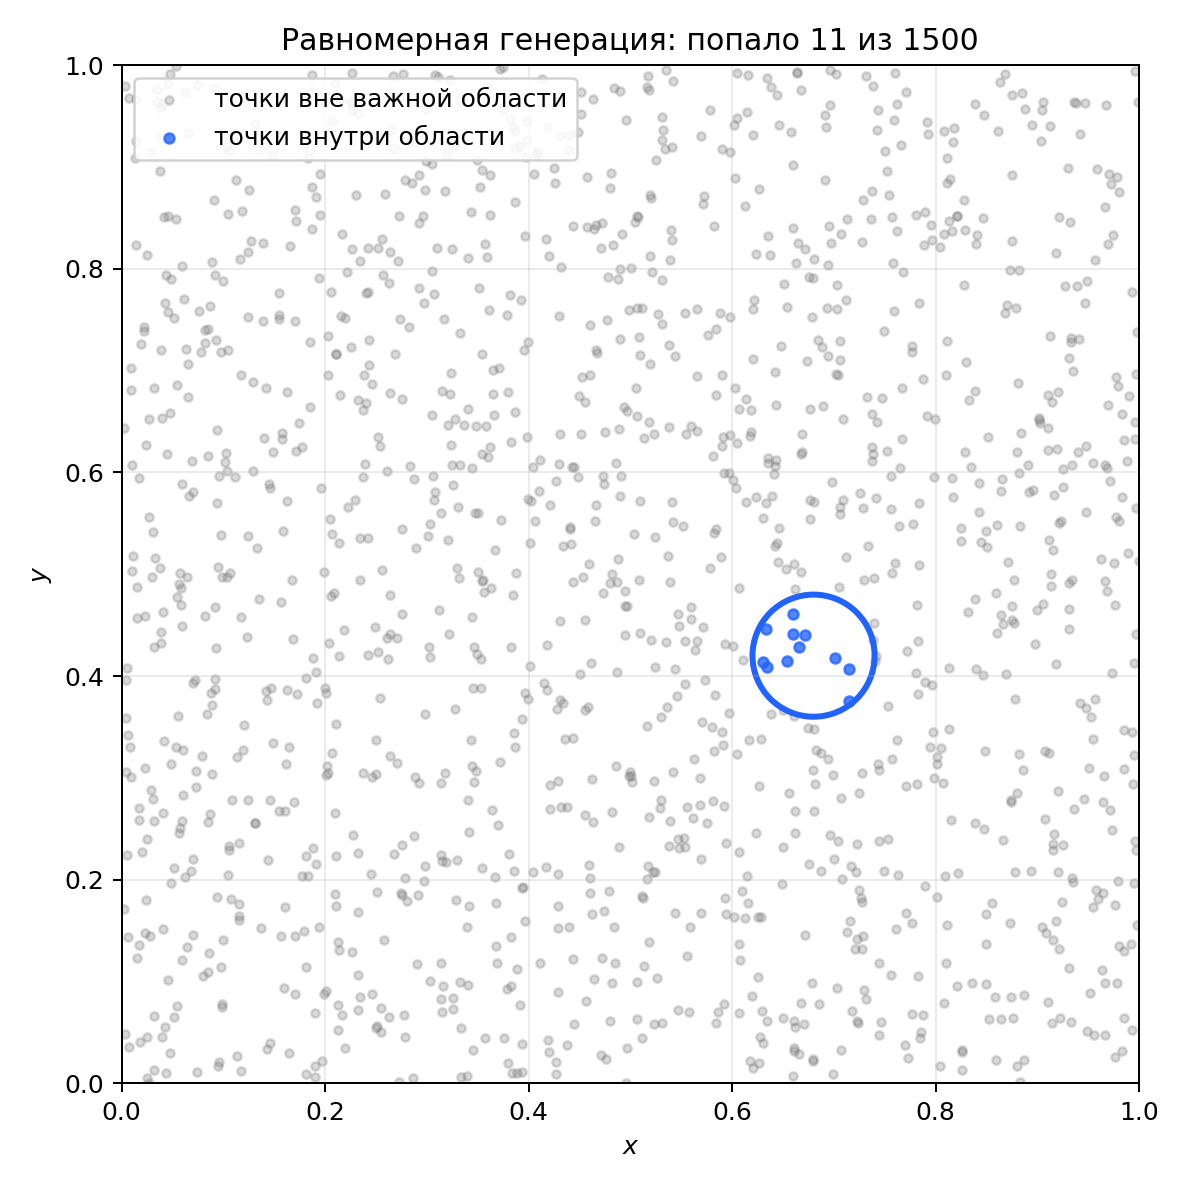
\includegraphics[width=0.74\linewidth,height=\textheight,keepaspectratio,alt={Равномерная выборка и выборка по важности}]{assets/figures/mc_rare_uniform.png}

\end{center}

\noindent\begin{minipage}[c]{\dimexpr\linewidth-30mm\relax}

\textbf{Интерактив}. \textbf{Равномерная выборка и выборка по важности}

При равномерной генерации малая доля точек попадает в важную область.

\end{minipage}\hfill\begin{minipage}[c]{26mm}\centering

\href{https://neutrinohit.github.io/statistical-analysis-course/ru/book/chapters/08_monte_carlo_method.html\#interactive-monte-carlo-importance-sampling}{
\includegraphics[width=24mm,height=\textheight,keepaspectratio,alt={QR-код интерактива}]{assets/qr/monte-carlo-importance-sampling.png}}

\end{minipage}

\end{semanticpdfbox}

\begin{figure}

\centering{

\pandocbounded{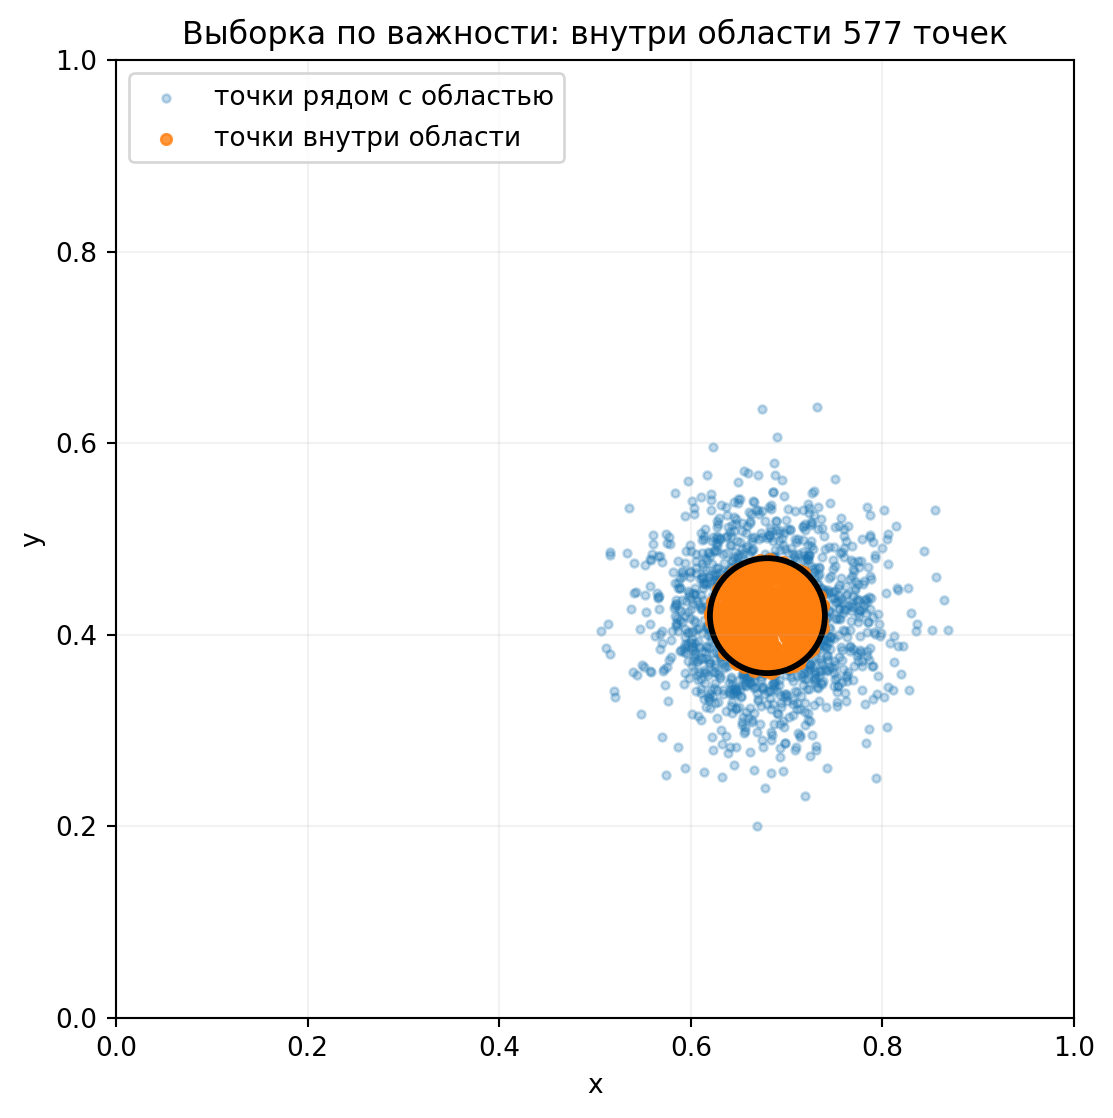
\includegraphics[keepaspectratio]{chapters/../assets/figures/mc_importance_sampling.png}}

}

\caption{\label{fig-ch8-importance-sampling}Выборка по важности
сосредоточивает точки вблизи области, которая даёт основной вклад в
интеграл}

\end{figure}%

\begin{figure}

\centering{

\pandocbounded{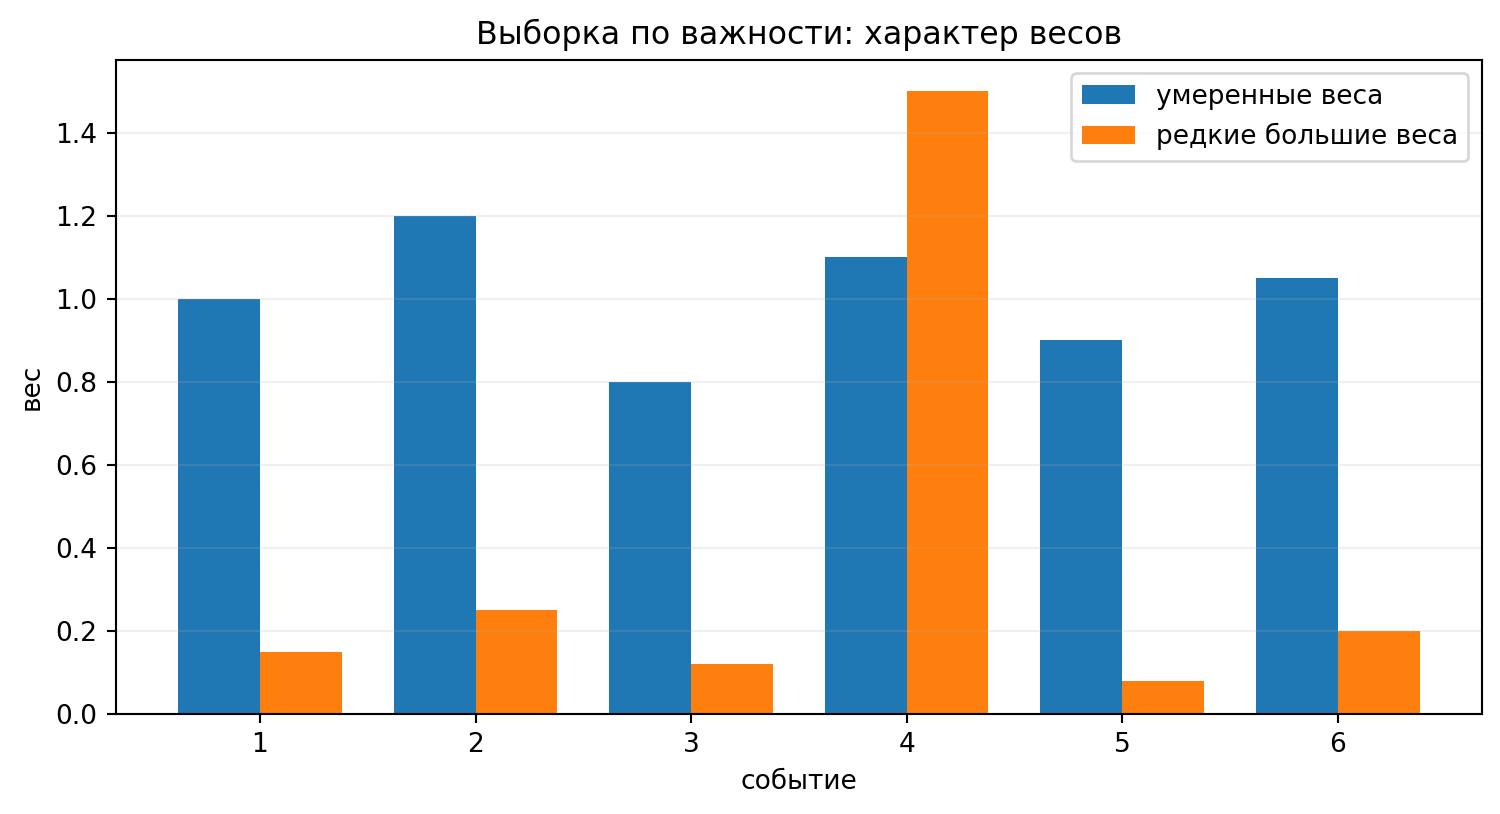
\includegraphics[keepaspectratio]{chapters/../assets/figures/mc_weights_good_bad.png}}

}

\caption{\label{fig-ch8-weight-dispersion}Умеренные веса дают много
сопоставимых вкладов; редкие события с очень большими весами увеличивают
дисперсию оценки}

\end{figure}%

\section{VEGAS: адаптивная выборка по
важности}\label{vegas-ux430ux434ux430ux43fux442ux438ux432ux43dux430ux44f-ux432ux44bux431ux43eux440ux43aux430-ux43fux43e-ux432ux430ux436ux43dux43eux441ux442ux438}

Для ручного выбора \(q(\mathbf x)\) надо заранее знать важную область.
Алгоритм VEGAS строит приближение к такой плотности по первым итерациям
расчёта {[}2{]}. В каждой координате он сгущает сетку там, где интегранд
вносит большой вклад. Полученная плотность имеет приближённо
разделяющийся вид

\begin{equation}\protect\phantomsection\label{eq-ch8-vegas-separable-density}{
q(\mathbf x)=\prod_{i=1}^{d}q_i(x_i).
}\end{equation}

\begin{figure}

\centering{

\pandocbounded{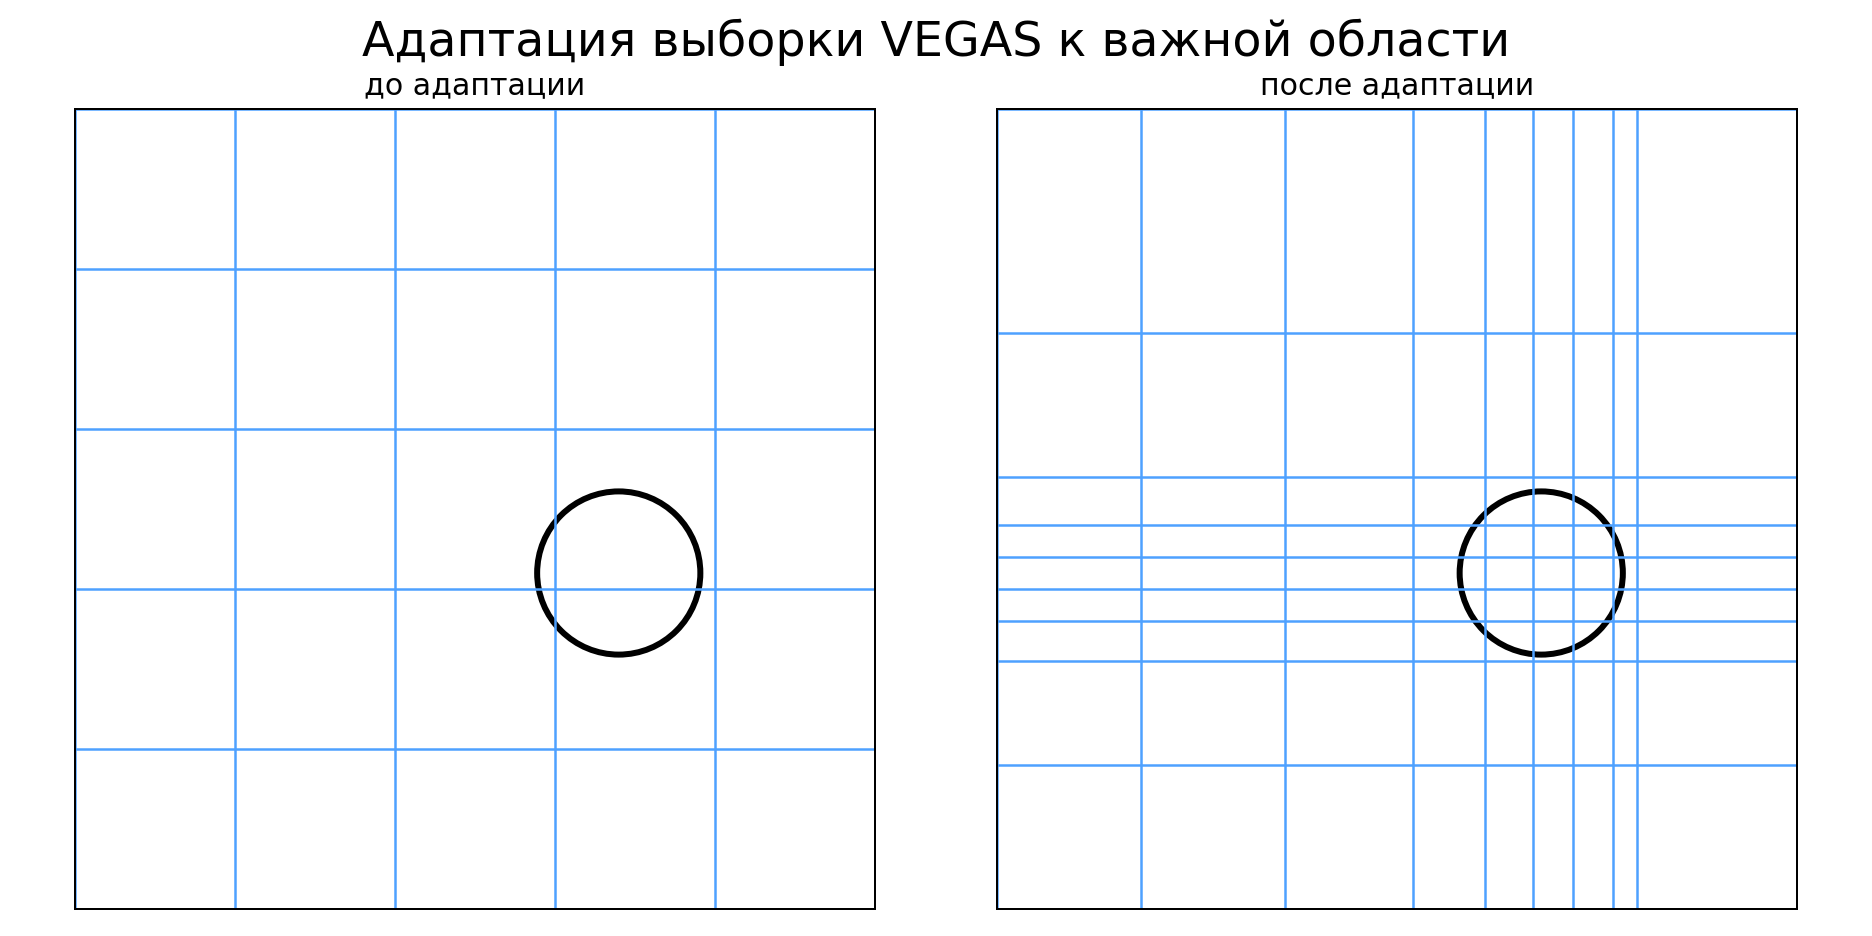
\includegraphics[keepaspectratio]{chapters/../assets/figures/mc_vegas_adaptation.png}}

}

\caption{\label{fig-ch8-vegas-adaptation}После нескольких итераций VEGAS
располагает больше интервалов в области большого вклада}

\end{figure}%

VEGAS сохраняет асимптотический закон \(1/\sqrt N\). Выигрыш получается
за счёт меньшей дисперсии. Разделяющаяся плотность хорошо описывает
пики, положение которых видно по отдельным координатам. Узкий
диагональный гребень или несколько далеко разнесённых пиков представляют
более трудную задачу.

\subsection{Контрольный восьмимерный
интеграл}\label{ux43aux43eux43dux442ux440ux43eux43bux44cux43dux44bux439-ux432ux43eux441ux44cux43cux438ux43cux435ux440ux43dux44bux439-ux438ux43dux442ux435ux433ux440ux430ux43b}

Рассмотрим произведение нормированных гауссовых плотностей в единичном
гиперкубе:

\begin{equation}\protect\phantomsection\label{eq-ch8-vegas-test-integrand}{
f(\mathbf x)=
\prod_{i=1}^{8}
\frac{1}{\sqrt{2\pi}\sigma}
\exp\!\left[-\frac{(x_i-\mu_i)^2}{2\sigma^2}\right],
\qquad 0\leq x_i\leq1,
}\end{equation}

где \(\sigma=0.10\), а центры равны

\begin{equation}\protect\phantomsection\label{eq-ch8-vegas-test-centres}{
\boldsymbol\mu=
(0.63,0.37,0.58,0.42,0.69,0.31,0.54,0.46).
}\end{equation}

Точный интеграл находится как произведение восьми одномерных гауссовых
интегралов:

\begin{equation}\protect\phantomsection\label{eq-ch8-vegas-test-exact}{
I_{\mathrm{exact}}=0.9978196359.
}\end{equation}

Простой Монте-Карло с одним и тем же начальным числом даёт результаты из
таблицы \ref{tbl-ch8-plain-monte-carlo}.

\begin{longtable}[]{@{}rr@{}}
\caption{Равномерный метод Монте-Карло для восьмимерного
интеграла}\label{tbl-ch8-plain-monte-carlo}\tabularnewline
\toprule\noalign{}
\(N\) & \(\widehat I_N\) \\
\midrule\noalign{}
\endfirsthead
\toprule\noalign{}
\(N\) & \(\widehat I_N\) \\
\midrule\noalign{}
\endhead
\bottomrule\noalign{}
\endlastfoot
\(10^4\) & \(0.946\pm0.48\) \\
\(10^5\) & \(0.864\pm0.13\) \\
\(10^6\) & \(1.001\pm0.061\) \\
\end{longtable}

Миллион точек всё ещё даёт ошибку около шести процентов: почти вся
равномерная выборка проходит мимо узкого пика. Тензорная квадратура
Гаусса---Лежандра сходится, но число вызовов функции растёт как \(m^8\).

\begin{longtable}[]{@{}rrr@{}}
\caption{Тензорная квадратура для восьмимерного
интеграла}\label{tbl-ch8-tensor-quadrature}\tabularnewline
\toprule\noalign{}
Узлов на координату \(m\) & Всего узлов \(m^8\) & Результат \\
\midrule\noalign{}
\endfirsthead
\toprule\noalign{}
Узлов на координату \(m\) & Всего узлов \(m^8\) & Результат \\
\midrule\noalign{}
\endhead
\bottomrule\noalign{}
\endlastfoot
3 & 6 561 & 0.589 \\
5 & 390 625 & 0.722 \\
7 & 5 764 801 & 0.963 \\
\end{longtable}

Числа в обеих таблицах получены скриптом
\texttt{shared/notebooks/mc\_vegas\_demo.py} с начальным состоянием
12345. После восьми адаптационных итераций по 20 000 точек и десяти
рабочих итераций по 50 000 точек VEGAS даёт

\begin{equation}\protect\phantomsection\label{eq-ch8-vegas-test-result}{
\widehat I_{\mathrm{VEGAS}}=0.99787\pm0.00053.
}\end{equation}

Этот пример специально удобен для VEGAS: интегранд раскладывается в
произведение функций отдельных координат. Для нового интеграла результат
проверяют независимыми запусками, увеличением числа точек и сравнением с
более грубым методом. Очень узкий пик алгоритм может не встретить на
первых итерациях, а значит, и не научиться генерировать точки в его
окрестности.

\section{Псевдоэксперименты}\label{ux43fux441ux435ux432ux434ux43eux44dux43aux441ux43fux435ux440ux438ux43cux435ux43dux442ux44b}

Псевдоэксперимент --- одна искусственная реализация измерения при
заданной модели. В простом случае достаточно сгенерировать одно число. В
полном анализе последовательно выполняются генерация физического
процесса, моделирование детектора, реконструкция, отбор и та же
статистическая процедура, которая применяется к данным.

Ансамбль псевдоэкспериментов позволяет найти:

\begin{itemize}
\tightlist
\item
  смещение и дисперсию оценки параметра;
\item
  распределение статистики теста;
\item
  покрытие доверительного интервала;
\item
  ожидаемую чувствительность эксперимента;
\item
  долю неудачных или нестабильных подгонок;
\item
  изменение результата при систематических вариациях модели.
\end{itemize}

Каждый такой вывод относится к модели и значениям параметров, при
которых был сгенерирован ансамбль.

\subsection{Возвращаемся к счётному
эксперименту}\label{interactive-monte-carlo-counting-experiment}

Для модели из формулы \ref{eq-ch8-counting-model} один псевдоэксперимент
состоит из генерации \(N\sim\operatorname{Pois}(s+b)\) и вычисления
\(\widehat s=N-b\). Повторив эти действия несколько тысяч раз, получим
распределение оценки.

\begin{semanticpdfbox}[breakable=false]

\begin{center}

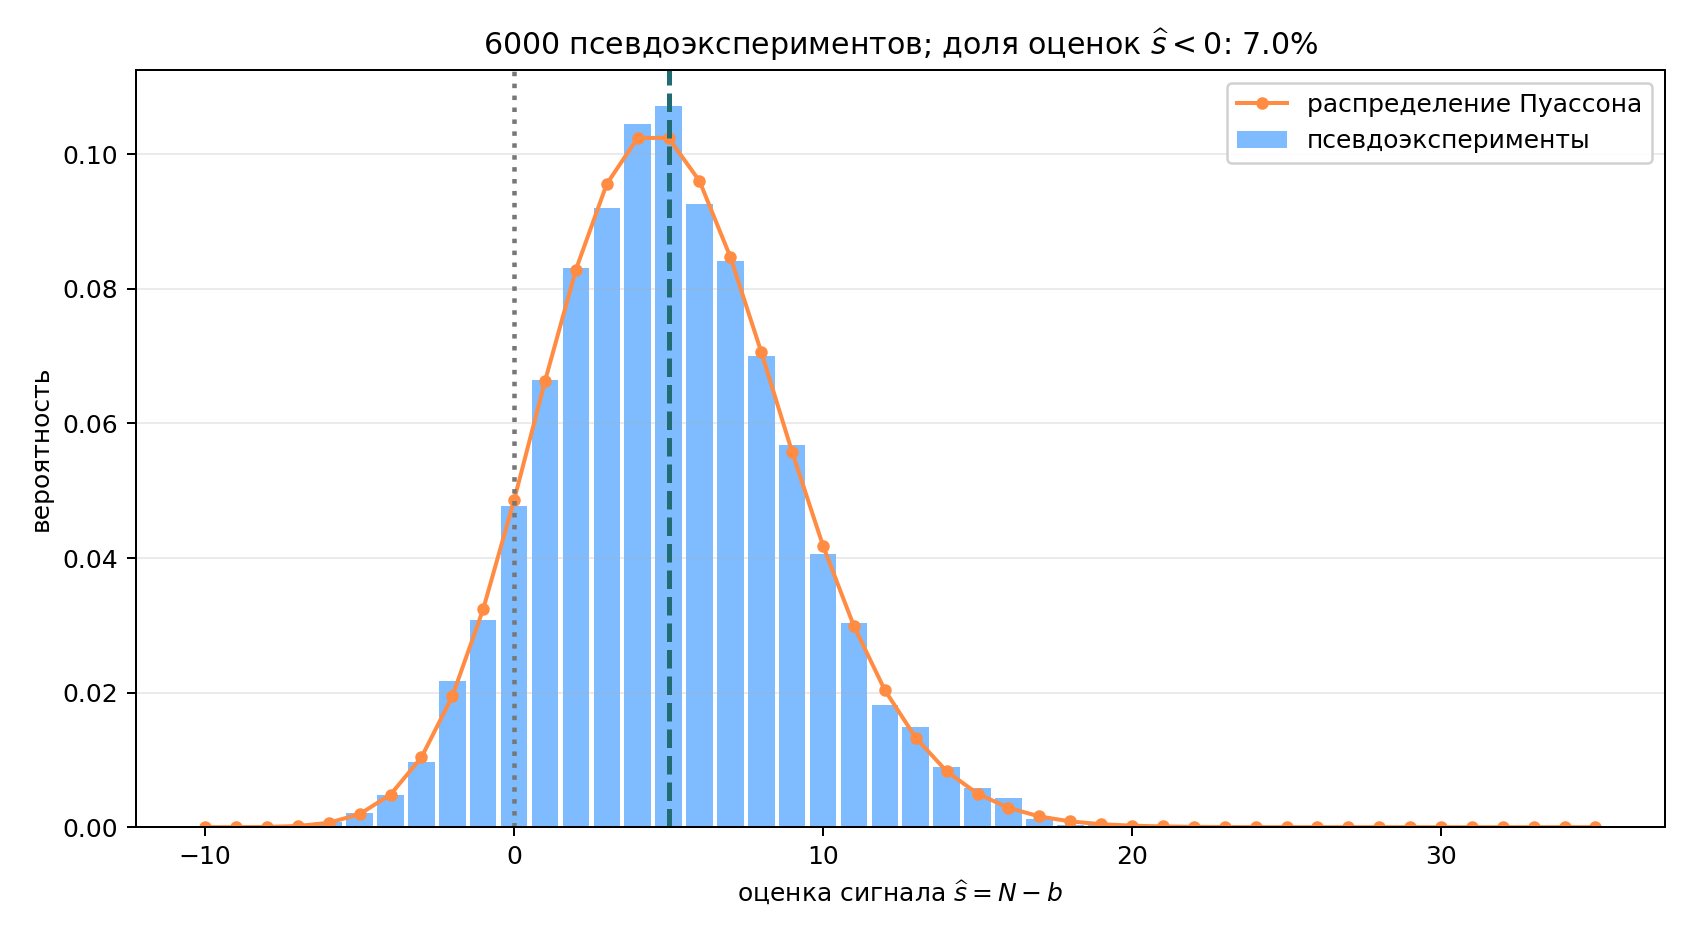
\includegraphics[width=0.74\linewidth,height=\textheight,keepaspectratio,alt={Ансамбль счётных экспериментов}]{assets/figures/mc_counting_pseudoexperiments.png}

\end{center}

\noindent\begin{minipage}[c]{\dimexpr\linewidth-30mm\relax}

\textbf{Интерактив}. \textbf{Ансамбль счётных экспериментов}

При \(s=5\) и \(b=10\) среднее распределения равно пяти, а около семи
процентов псевдоэкспериментов дают \(\widehat s<0\).

\end{minipage}\hfill\begin{minipage}[c]{26mm}\centering

\href{https://neutrinohit.github.io/statistical-analysis-course/ru/book/chapters/08_monte_carlo_method.html\#interactive-monte-carlo-counting-experiment}{
\includegraphics[width=24mm,height=\textheight,keepaspectratio,alt={QR-код интерактива}]{assets/qr/monte-carlo-counting-experiment.png}}

\end{minipage}

\end{semanticpdfbox}

Отрицательное \(\widehat s\) не означает отрицательного числа физических
событий. Так проявляется флуктуация оценки \(N-b\). Статистическая
процедура должна уметь работать и с такими реализациями; удаление их из
ансамбля изменит среднее и нарушит свойства метода.

Реальный эксперимент даёт одну точку из показанного распределения.
Увеличение числа псевдоэкспериментов точнее определяет это
распределение, но не уменьшает разброс результата одного реального
измерения.

\section{Моделирование полного
эксперимента}\label{ux43cux43eux434ux435ux43bux438ux440ux43eux432ux430ux43dux438ux435-ux43fux43eux43bux43dux43eux433ux43e-ux44dux43aux441ux43fux435ux440ux438ux43cux435ux43dux442ux430}

В физике частиц и нейтрино один псевдоэксперимент может опираться на
длинную цепочку моделирования:

\begin{enumerate}
\def\labelenumi{\arabic{enumi}.}
\tightlist
\item
  генератор задаёт процесс, типы частиц и их кинематику;
\item
  моделируется прохождение частиц через вещество, потери энергии и
  вторичные частицы;
\item
  вычисляется отклик сенсоров и электроники;
\item
  программа реконструкции восстанавливает энергию, координаты и тип
  события;
\item
  применяются триггер, критерии качества и отбор анализа.
\end{enumerate}

Каждый этап содержит приближения. Их проверяют по контрольным данным, а
оставшиеся расхождения входят в систематическую неопределённость.

\begin{semanticpdfbox}[breakable=false]

\noindent\begin{minipage}[c]{\dimexpr\linewidth-30mm\relax}

\textbf{Интерактив}. \textbf{Моделирование оптических фотонов в Daya Bay
и JUNO}

В ролике Саймона Блита показана работа Opticks: распространение
оптических фотонов рассчитывается на графическом процессоре для
геометрий детекторов Daya Bay и JUNO. Описание проекта опубликовано на
странице автора {[}3{]}.

\end{minipage}\hfill\begin{minipage}[c]{26mm}\centering

\href{https://juno.ihep.ac.cn/~blyth/}{
\includegraphics[width=24mm,height=\textheight,keepaspectratio,alt={QR-код интерактива}]{assets/qr/opticks-video.png}}

\end{minipage}

\end{semanticpdfbox}

\subsection{Матрица
отклика}\label{ux43cux430ux442ux440ux438ux446ux430-ux43eux442ux43aux43bux438ux43aux430}

Пусть истинный спектр разбит на бины. Элемент матрицы отклика

\begin{equation}\protect\phantomsection\label{eq-ch8-response-matrix-element}{
R_{ji}
=P(\text{событие восстановлено в бине }j
\mid\text{истинный бин }i)
}\end{equation}

оценивается по моделированию. Если истинный спектр равен \(\mathbf t\),
то ожидаемый восстановленный спектр имеет вид

\begin{equation}\protect\phantomsection\label{eq-ch8-response-matrix-folding}{
\boxed{\mathbf r=R\mathbf t.}
}\end{equation}

Диагональные элементы описывают правильную реконструкцию бина,
внедиагональные --- миграции. Сумма элементов столбца может быть меньше
единицы: часть событий теряется из-за геометрического аксептанса,
порогов и отбора.

\subsection{Эффективность
отбора}\label{ux44dux444ux444ux435ux43aux442ux438ux432ux43dux43eux441ux442ux44c-ux43eux442ux431ux43eux440ux430}

Если из \(N_{\mathrm{gen}}\) сгенерированных событий прошло отбор
\(N_{\mathrm{sel}}\), оценка эффективности равна

\begin{equation}\protect\phantomsection\label{eq-ch8-selection-efficiency}{
\widehat\varepsilon
=\frac{N_{\mathrm{sel}}}{N_{\mathrm{gen}}}.
}\end{equation}

Для независимых событий с единичными весами

\begin{equation}\protect\phantomsection\label{eq-ch8-selected-binomial-model}{
N_{\mathrm{sel}}
\sim\operatorname{Bin}(N_{\mathrm{gen}},\varepsilon),
}\end{equation}

поэтому стандартную ошибку обычно оценивают как

\begin{equation}\protect\phantomsection\label{eq-ch8-selection-efficiency-error}{
\boxed{
\sigma_{\widehat\varepsilon}
\simeq
\sqrt{\frac{
\widehat\varepsilon(1-\widehat\varepsilon)
}{N_{\mathrm{gen}}}}.
}
}\end{equation}

У этой формулы хорошо видны границы применимости. Если все события
прошли отбор, она даёт \(\widehat\varepsilon=1\) и нулевую ошибку. Из
конечной выборки следует лишь, что в ней не встретился ни один отказ.
Следующее событие пройти отбор не обязано. Вблизи физических границ
\(0\leq\varepsilon\leq1\) нужны интервальные методы; они рассматриваются
в следующих главах.

При наличии весов биномиальная модель уже неприменима в таком виде.
Тогда проверяют суммы весов, суммы квадратов весов и эффективный размер
выборки из формулы \ref{eq-ch8-effective-sample-size}.

\section{Как проверять
расчёт}\label{ux43aux430ux43a-ux43fux440ux43eux432ux435ux440ux44fux442ux44c-ux440ux430ux441ux447ux451ux442}

Расчёт Монте-Карло начинают с задач, для которых известен ответ.
Проверяют нормировку, средние, дисперсии, корреляции и предельные
значения параметров. Результаты независимых запусков должны быть
совместимы, а численная ошибка --- убывать с ожидаемой скоростью при
увеличении статистики.

Если из псевдоэксперимента восстанавливается параметр \(\theta\), на
ансамбле с известным истинным значением вычисляют смещение

\begin{equation}\protect\phantomsection\label{eq-ch8-estimator-bias}{
\operatorname{bias}(\widehat\theta)
=\mathbb E[\widehat\theta]-\theta
}\end{equation}

и дисперсию

\begin{equation}\protect\phantomsection\label{eq-ch8-estimator-variance}{
\operatorname{Var}(\widehat\theta)
=\mathbb E\!\left[
(\widehat\theta-\mathbb E[\widehat\theta])^2
\right].
}\end{equation}

Оценка не обязана быть точно несмещённой при конечной статистике. Её
смещение должно быть измерено и сопоставлено с требуемой точностью
анализа.

\begin{booknote}

Здесь участвуют два разных разброса. Физическая статистическая
неопределённость описывает возможные результаты одного реального
эксперимента. Численная ошибка Монте-Карло показывает, насколько точно
конечная симуляция оценивает это распределение. Большее число
псевдоэкспериментов уменьшает вторую ошибку. Первая определяется объёмом
реальных данных.

\end{booknote}

Для взвешенной выборки отдельно проверяют распределение весов и
\(N_{\mathrm{eff}}\). Для адаптивного интегрирования сравнивают итерации
и независимые начальные состояния. Для полного моделирования тестируют
каждый этап цепочки и сопоставляют контрольные распределения с данными.

Вероятностная модель, конфигурация, версии программ и начальные
состояния генераторов являются частью результата. Без них численный
ответ трудно воспроизвести, а иногда невозможно даже понять, что именно
было вычислено.

\section{Когда нужен другой
метод}\label{ux43aux43eux433ux434ux430-ux43dux443ux436ux435ux43d-ux434ux440ux443ux433ux43eux439-ux43cux435ux442ux43eux434}

Для одномерного интеграла с гладкой известной функцией квадратура обычно
быстрее простого Монте-Карло. Редкие области требуют выборки по важности
или специализированной генерации. Для сложных многомерных распределений
параметров используют методы Монте-Карло по марковским цепям и вложенную
выборку. Полное моделирование детектора иногда заменяют быстрой
параметризацией или суррогатной моделью.

Выбор метода определяется задачей и стоимостью одного вычисления.
Результат Монте-Карло считается надёжным после проверки реализации,
сходимости и модели, по которой он получен.

\begin{bookchaptersummary}[Итоги главы]

\begin{itemize}
\tightlist
\item
  Метод Монте-Карло строит численный ансамбль реализаций заданной
  модели.
\item
  Равномерные псевдослучайные числа преобразуются в нужное распределение
  обратной функцией, методом отбора или специальным алгоритмом.
\item
  Ошибка простого интегрирования убывает как \(1/\sqrt N\); в большой
  размерности это часто выгоднее регулярной сетки.
\item
  Выборка по важности и VEGAS уменьшают дисперсию, направляя вычисления
  в области большого вклада.
\item
  Псевдоэксперименты позволяют проверить всю статистическую процедуру от
  генерации данных до оценки параметра.
\item
  Статистическая неопределённость реального эксперимента и численная
  ошибка конечной симуляции являются разными величинами.
\end{itemize}

\end{bookchaptersummary}

\section{Задачи}\label{ux437ux430ux434ux430ux447ux438-7}

\begin{semanticpdfbox}[colback=BookCoralSoft,borderline west={1.2mm}{0pt}{BookCoral},breakable=false]

\noindent{\sffamily\bfseries\fontsize{11.2}{13.5}\selectfont Задача 1. Обратная функция распределения}\par\nopagebreak[4]\vspace{1.2mm}

Пусть \[
U\sim\mathrm U(0,1).
\]

\begin{enumerate}
\def\labelenumi{\arabic{enumi}.}
\tightlist
\item
  Покажите, что \[
  X=-\frac{1}{\lambda}\ln(1-U)
  \] имеет экспоненциальное распределение с параметром \(\lambda\).
\item
  Сгенерируйте выборку \(X\) и сравните гистограмму с аналитической
  плотностью.
\item
  Проверьте выборочные среднее и дисперсию.
\end{enumerate}

\end{semanticpdfbox}

\begin{semanticpdfbox}[colback=BookCoralSoft,borderline west={1.2mm}{0pt}{BookCoral},breakable=false]

\noindent{\sffamily\bfseries\fontsize{11.2}{13.5}\selectfont Задача 2. Метод отбора}\par\nopagebreak[4]\vspace{1.2mm}

Требуется генерировать плотность \[
f(x)=6x(1-x),
\qquad 0\le x\le1.
\]

\begin{enumerate}
\def\labelenumi{\arabic{enumi}.}
\tightlist
\item
  Найдите максимум \(f(x)\).
\item
  Постройте алгоритм отбора из равномерного распределения.
\item
  Вычислите теоретическую эффективность алгоритма.
\item
  Проверьте её численно.
\end{enumerate}

\end{semanticpdfbox}

\begin{semanticpdfbox}[colback=BookCoralSoft,borderline west={1.2mm}{0pt}{BookCoral},breakable=false]

\noindent{\sffamily\bfseries\fontsize{11.2}{13.5}\selectfont Задача 3. Интегрирование методом Монте-Карло}\par\nopagebreak[4]\vspace{1.2mm}

Вычислите \[
I=\int_0^1\frac{4}{1+x^2}\,dx=\pi
\] методом Монте-Карло.

\begin{enumerate}
\def\labelenumi{\arabic{enumi}.}
\tightlist
\item
  Запишите оценку \(\widehat I_N\).
\item
  Оцените её статистическую ошибку по выборке.
\item
  Исследуйте зависимость ошибки от \(N\).
\item
  Покажите численно, что ошибка убывает приблизительно как \(N^{-1/2}\).
\end{enumerate}

\end{semanticpdfbox}

\begin{semanticpdfbox}[colback=BookCoralSoft,borderline west={1.2mm}{0pt}{BookCoral},breakable=false]

\noindent{\sffamily\bfseries\fontsize{11.2}{13.5}\selectfont Задача 4. Редкое событие и выборка по важности}\par\nopagebreak[4]\vspace{1.2mm}

Требуется оценить вероятность \[
p=P(Z>4),
\qquad
Z\sim\mathrm N(0,1).
\]

\begin{enumerate}
\def\labelenumi{\arabic{enumi}.}
\tightlist
\item
  Оцените \(p\) наивной генерацией из стандартного гаусса.
\item
  Объясните, почему для устойчивой оценки требуется очень большая
  выборка.
\item
  Предложите распределение \(q(z)\), чаще генерирующее область \(z>4\).
\item
  Запишите соответствующий вес \(w(z)=f(z)/q(z)\).
\item
  Сравните дисперсии двух оценок.
\end{enumerate}

\end{semanticpdfbox}

\begin{semanticpdfbox}[colback=BookCoralSoft,borderline west={1.2mm}{0pt}{BookCoral},breakable=false]

\noindent{\sffamily\bfseries\fontsize{11.2}{13.5}\selectfont Задача 5. Псевдоэксперименты для счётного эксперимента}\par\nopagebreak[4]\vspace{1.2mm}

Пусть \[
N\sim\operatorname{Pois}(s+b),
\qquad
\widehat s=N-b,
\] где фон \(b\) известен точно.

\begin{enumerate}
\def\labelenumi{\arabic{enumi}.}
\tightlist
\item
  Найдите аналитические \(\mathbb E[\widehat s]\) и
  \(\operatorname{Var}(\widehat s)\).
\item
  Постройте ансамбль псевдоэкспериментов.
\item
  Сравните выборочные среднее и дисперсию с аналитическими значениями.
\item
  Оцените вероятность получить \(\widehat s<0\).
\end{enumerate}

\end{semanticpdfbox}

\begin{semanticpdfbox}[colback=BookCoralSoft,borderline west={1.2mm}{0pt}{BookCoral},breakable=false]

\noindent{\sffamily\bfseries\fontsize{11.2}{13.5}\selectfont Задача 6. Нелинейное распространение ошибки}\par\nopagebreak[4]\vspace{1.2mm}

Пусть коррелированные величины имеют распределение \[
\begin{pmatrix}X\\Y\end{pmatrix}
\sim
\mathrm N\!\left[
\begin{pmatrix}10\\5\end{pmatrix},
\begin{pmatrix}
\sigma_X^2 & \rho\sigma_X\sigma_Y\\
\rho\sigma_X\sigma_Y & \sigma_Y^2
\end{pmatrix}
\right].
\]

Для отношения \[
R=\frac{X}{Y}
\] сравните:

\begin{enumerate}
\def\labelenumi{\arabic{enumi}.}
\tightlist
\item
  линейную оценку ошибки;
\item
  стандартное отклонение выборки Монте-Карло;
\item
  центральный квантильный интервал \([q_{0.16},q_{0.84}]\).
\end{enumerate}

Исследуйте зависимость результатов от \(\sigma_Y\) и \(\rho\).

\end{semanticpdfbox}

\begin{semanticpdfbox}[colback=BookCoralSoft,borderline west={1.2mm}{0pt}{BookCoral},breakable=false]

\noindent{\sffamily\bfseries\fontsize{11.2}{13.5}\selectfont Задача 7. Эффективность отбора}\par\nopagebreak[4]\vspace{1.2mm}

Из \(N_{\mathrm{gen}}=10\,000\) сгенерированных событий отбор прошло
\(N_{\mathrm{sel}}=730\).

\begin{enumerate}
\def\labelenumi{\arabic{enumi}.}
\tightlist
\item
  Оцените эффективность отбора.
\item
  Оцените её биномиальную статистическую ошибку.
\item
  Сколько событий требуется сгенерировать, чтобы относительная ошибка
  эффективности была меньше \(1\%\)?
\item
  Обсудите, как изменится задача при наличии весов событий.
\end{enumerate}

\end{semanticpdfbox}

\begin{semanticpdfbox}[colback=BookCoralSoft,borderline west={1.2mm}{0pt}{BookCoral},breakable=false]

\noindent{\sffamily\bfseries\fontsize{11.2}{13.5}\selectfont Задача 8. Эффективный размер выборки}\par\nopagebreak[4]\vspace{1.2mm}

Для взвешенной выборки определено \[
N_{\mathrm{eff}}
=
\frac{(\sum_k w_k)^2}{\sum_k w_k^2}.
\]

\begin{enumerate}
\def\labelenumi{\arabic{enumi}.}
\tightlist
\item
  Покажите, что при одинаковых весах \(N_{\mathrm{eff}}=N\).
\item
  Найдите \(N_{\mathrm{eff}}\) для весов \[
  (1,1,1,1,6).
  \]
\item
  Сравните результат с фактическим числом событий.
\item
  Объясните, почему большая вариация весов ухудшает статистическую
  точность.
\end{enumerate}

\end{semanticpdfbox}

\section*{Литература}\label{ux43bux438ux442ux435ux440ux430ux442ux443ux440ux430-7}
\addcontentsline{toc}{section}{Литература}

\markright{Литература}

\protect\phantomsection\label{refs}
\begin{CSLReferences}{0}{0}
\bibitem[\citeproctext]{ref-metropolisUlam1949}
{[}1{]} Metropolis, N. и Ulam, S. The {Monte Carlo} Method.
\emph{Journal of the American Statistical Association}, \textbf{44},
335--341. 1949.
doi:\href{https://doi.org/10.1080/01621459.1949.10483310}{10.1080/01621459.1949.10483310}.

\bibitem[\citeproctext]{ref-lepage1978vegas}
{[}2{]} Lepage, G. P. A New Algorithm for Adaptive Multidimensional
Integration. \emph{Journal of Computational Physics}, \textbf{27},
192--203. 1978.
doi:\href{https://doi.org/10.1016/0021-9991(78)90004-9}{10.1016/0021-9991(78)90004-9}.

\bibitem[\citeproctext]{ref-blythOpticks}
{[}3{]} Blyth, S. C. Opticks: {GPU} Optical Photon Simulation.
\url{https://juno.ihep.ac.cn/~blyth/}.

\end{CSLReferences}

\chapter{Правдоподобие и оценки максимального
правдоподобия}\label{ux43fux440ux430ux432ux434ux43eux43fux43eux434ux43eux431ux438ux435-ux438-ux43eux446ux435ux43dux43aux438-ux43cux430ux43aux441ux438ux43cux430ux43bux44cux43dux43eux433ux43e-ux43fux440ux430ux432ux434ux43eux43fux43eux434ux43eux431ux438ux44f}

\bookchapteropeningcontents

\begin{bookchapteropening}[Аннотация]

В этой главе мы перейдём от вероятностной модели данных к оценке её
параметров. Начнём с калибровки эффективности детектора, введём функцию
правдоподобия и найдём её максимум. Затем тот же метод применим к
пуассоновскому счёту и гауссову распределению. Последний пример покажет,
что оценка максимального правдоподобия может быть смещённой.

\end{bookchapteropening}

\section{Физическая задача: эффективность
регистрации}\label{ux444ux438ux437ux438ux447ux435ux441ux43aux430ux44f-ux437ux430ux434ux430ux447ux430-ux44dux444ux444ux435ux43aux442ux438ux432ux43dux43eux441ux442ux44c-ux440ux435ux433ux438ux441ux442ux440ux430ux446ux438ux438}

Перед исследуемым детектором установлен другой прибор, который отмечает
прохождение заряженной частицы. За время калибровки он зарегистрировал
\(N=20\) частиц. Исследуемый детектор сработал для \(k=7\) из них.
Требуется оценить его эффективность \(\varepsilon\). Ошибками первого
прибора и случайными совпадениями пока пренебрежём.

Каждая частица даёт один из двух результатов: детектор сработал или не
сработал. Если результаты независимы, а эффективность во время
калибровки постоянна, число зарегистрированных частиц имеет биномиальное
распределение:

\begin{equation}\protect\phantomsection\label{eq-ch9-efficiency-model}{
K\sim\operatorname{Bin}(N,\varepsilon).
}\end{equation}

Первая оценка напрашивается сама:

\begin{equation}\protect\phantomsection\label{eq-ch9-efficiency-first-estimate}{
\widehat\varepsilon=\frac{k}{N}=\frac7{20}=0.35.
}\end{equation}

Почему именно эта оценка? Что означает её шляпка? Как изменится вывод,
если детектор сработает семь раз из двадцати или семьдесят раз из
двухсот? И что делать, если число зарегистрированных событий
складывается из сигнала и известного фона? Для ответа запишем функцию
правдоподобия.

\section{Оценка и её
значение}\label{ux43eux446ux435ux43dux43aux430-ux438-ux435ux451-ux437ux43dux430ux447ux435ux43dux438ux435}

Пусть данные описываются распределением

\begin{equation}\protect\phantomsection\label{eq-ch9-statistical-model}{
X\sim f(x\mid\boldsymbol\theta),
}\end{equation}

где \(\boldsymbol\theta\) --- параметр или набор параметров модели. Это
может быть эффективность детектора, среднее число событий, масса
частицы, сечение процесса или коэффициент корреляции.

В частотном подходе \(\boldsymbol\theta\) фиксирован, но неизвестен. До
эксперимента случайны данные. \textbf{Оценкой} параметра называется
правило, которое ставит данным в соответствие число или вектор чисел:

\begin{equation}\protect\phantomsection\label{eq-ch9-estimator-definition}{
\widehat{\boldsymbol\theta}
=T(X_1,\ldots,X_N).
}\end{equation}

После подстановки конкретной выборки получается значение оценки:

\begin{equation}\protect\phantomsection\label{eq-ch9-estimate-value}{
\widehat{\boldsymbol\theta}_{\mathrm{data}}
=T(x_1,\ldots,x_N).
}\end{equation}

Это различие понадобится дальше. В формуле
\ref{eq-ch9-estimator-definition} оценка является случайной величиной и
меняется от опыта к опыту. Число в формуле \ref{eq-ch9-estimate-value}
уже получено из данных.

\subsection{Один параметр --- разные
оценки}\label{ux43eux434ux438ux43d-ux43fux430ux440ux430ux43cux435ux442ux440-ux440ux430ux437ux43dux44bux435-ux43eux446ux435ux43dux43aux438}

Пусть \(X_1,\ldots,X_N\) имеют гауссово распределение со средним
\(\mu\). Оценивать \(\mu\) можно выборочным средним, медианой или,
например, полусуммой первого и последнего элементов выборки:

\begin{equation}\protect\phantomsection\label{eq-ch9-three-estimators}{
\widehat\mu_1=\frac1N\sum_{i=1}^{N}X_i,
\qquad
\widehat\mu_2=\operatorname{median}(X_1,\ldots,X_N),
\qquad
\widehat\mu_3=\frac{X_1+X_N}{2}.
}\end{equation}

Все три правила дают оценку одного параметра. При гауссовом
распределении они несмещённые, но разброс у них различен. Третья оценка,
кроме того, выбрасывает почти всю собранную информацию. Условие задачи
само по себе ещё не выбирает оценку. Нужен принцип, по которому этот
выбор будет сделан.

Точечная оценка даёт одно значение \(\widehat{\boldsymbol\theta}\).
Интервальная оценка задаёт область допустимых значений параметра. В этой
главе мы строим точечные оценки. Интервалы потребуют отдельной
статистической процедуры, к которой мы перейдём позже.

\section{Функция
правдоподобия}\label{ux444ux443ux43dux43aux446ux438ux44f-ux43fux440ux430ux432ux434ux43eux43fux43eux434ux43eux431ux438ux44f}

При заданном \(\boldsymbol\theta\) функция \(f(x\mid\boldsymbol\theta)\)
описывает распределение возможных данных. После эксперимента данные
\(\mathbf x\) фиксированы, а параметр остаётся неизвестным. Рассмотрим
ту же функцию как функцию параметра:

\begin{equation}\protect\phantomsection\label{eq-ch9-likelihood-definition}{
\boxed{
L(\boldsymbol\theta;\mathbf x)
=f(\mathbf x\mid\boldsymbol\theta)
}.
}\end{equation}

Она называется \textbf{функцией правдоподобия}. Вертикальная черта в
\(f(\mathbf x\mid\boldsymbol\theta)\) напоминает, что распределение
данных задаётся при фиксированных параметрах. Точка с запятой в
\(L(\boldsymbol\theta;\mathbf x)\) отделяет аргумент функции от уже
полученных данных.

\begin{longtable}[]{@{}
  >{\raggedright\arraybackslash}p{(\linewidth - 6\tabcolsep) * \real{0.2500}}
  >{\raggedright\arraybackslash}p{(\linewidth - 6\tabcolsep) * \real{0.2500}}
  >{\raggedright\arraybackslash}p{(\linewidth - 6\tabcolsep) * \real{0.2500}}
  >{\raggedright\arraybackslash}p{(\linewidth - 6\tabcolsep) * \real{0.2500}}@{}}
\caption{Вероятностная модель и функция правдоподобия используют одну
математическую функцию, но отвечают на разные
вопросы.}\label{tbl-ch9-probability-and-likelihood}\tabularnewline
\toprule\noalign{}
\begin{minipage}[b]{\linewidth}\raggedright
Функция
\end{minipage} & \begin{minipage}[b]{\linewidth}\raggedright
Фиксировано
\end{minipage} & \begin{minipage}[b]{\linewidth}\raggedright
Что меняется
\end{minipage} & \begin{minipage}[b]{\linewidth}\raggedright
Вопрос
\end{minipage} \\
\midrule\noalign{}
\endfirsthead
\toprule\noalign{}
\begin{minipage}[b]{\linewidth}\raggedright
Функция
\end{minipage} & \begin{minipage}[b]{\linewidth}\raggedright
Фиксировано
\end{minipage} & \begin{minipage}[b]{\linewidth}\raggedright
Что меняется
\end{minipage} & \begin{minipage}[b]{\linewidth}\raggedright
Вопрос
\end{minipage} \\
\midrule\noalign{}
\endhead
\bottomrule\noalign{}
\endlastfoot
\(f(\mathbf x\mid\boldsymbol\theta)\) & \(\boldsymbol\theta\) &
\(\mathbf x\) & Как распределены результаты повторных опытов? \\
\(L(\boldsymbol\theta;\mathbf x)\) & \(\mathbf x\) &
\(\boldsymbol\theta\) & Какие параметры лучше согласуются с этими
данными? \\
\end{longtable}

Правдоподобие не является распределением вероятности параметра. Для него
нет условия нормировки по \(\boldsymbol\theta\). Более того, множитель,
который не зависит от \(\boldsymbol\theta\), можно отбросить: положение
максимума и отношения значений \(L\) от этого не изменятся.

\subsection{Независимая
выборка}\label{ux43dux435ux437ux430ux432ux438ux441ux438ux43cux430ux44f-ux432ux44bux431ux43eux440ux43aux430}

Для независимых измерений совместное правдоподобие равно произведению:

\begin{equation}\protect\phantomsection\label{eq-ch9-independent-likelihood}{
L(\boldsymbol\theta)
=\prod_{i=1}^{N}f_i(x_i\mid\boldsymbol\theta).
}\end{equation}

Индекс у \(f_i\) допускает разные распределения или разные ошибки
отдельных измерений. Для одинаково распределённых величин все \(f_i\)
совпадают.

Произведение многих малых чисел быстро достигает машинного нуля. Поэтому
в вычислениях используют логарифм правдоподобия:

\begin{equation}\protect\phantomsection\label{eq-ch9-log-likelihood}{
\ell(\boldsymbol\theta)
=\ln L(\boldsymbol\theta)
=\sum_{i=1}^{N}\ln f_i(x_i\mid\boldsymbol\theta).
}\end{equation}

Логарифм монотонен, поэтому \(L\) и \(\ell\) достигают максимума при
одних и тех же параметрах. Независимые наборы данных добавляют к общей
функции по одному слагаемому:

\begin{equation}\protect\phantomsection\label{eq-ch9-combined-log-likelihood}{
\ell_{\mathrm{total}}(\boldsymbol\theta)
=\ell_1(\boldsymbol\theta)+\ell_2(\boldsymbol\theta)+\cdots.
}\end{equation}

В больших экспериментах результаты разных каналов и периодов набора
данных объединяются сложением соответствующих логарифмов.

\section{Метод максимального
правдоподобия}\label{ux43cux435ux442ux43eux434-ux43cux430ux43aux441ux438ux43cux430ux43bux44cux43dux43eux433ux43e-ux43fux440ux430ux432ux434ux43eux43fux43eux434ux43eux431ux438ux44f}

Оценка максимального правдоподобия выбирает параметры, при которых
полученные данные имеют наибольшее правдоподобие {[}1, 2{]}:

\begin{equation}\protect\phantomsection\label{eq-ch9-maximum-likelihood-estimator}{
\boxed{
\widehat{\boldsymbol\theta}_{\mathrm{ММП}}
=\underset{\boldsymbol\theta}{\operatorname{arg\,max}}\,
L(\boldsymbol\theta)
=\underset{\boldsymbol\theta}{\operatorname{arg\,max}}\,
\ell(\boldsymbol\theta)
}.
}\end{equation}

Если максимум находится внутри допустимой области, а функция гладкая, то
для одного параметра выполняются условия

\begin{equation}\protect\phantomsection\label{eq-ch9-interior-maximum-conditions}{
\left.
\frac{d\ell}{d\theta}
\right|_{\theta=\widehat\theta}=0,
\qquad
\left.
\frac{d^2\ell}{d\theta^2}
\right|_{\theta=\widehat\theta}<0.
}\end{equation}

Слово «внутри» здесь существенно. Если параметр ограничен, максимум
может оказаться на границе, где первая производная не равна нулю. Такой
случай мы увидим уже в биномиальной задаче.

\begin{semanticpdfbox}[colback=BookBiographySoft,borderline west={1.2mm}{0pt}{BookBiography},breakable=false]

\noindent\begin{minipage}[t]{30mm}\vspace{0pt}\centering

\href{https://commons.wikimedia.org/wiki/File:Youngronaldfisher2.JPG}{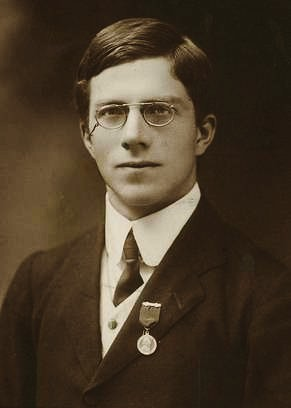
\includegraphics[width=28mm,height=\textheight,keepaspectratio,alt={Портрет молодого Рональда Эйлмера Фишера}]{assets/people/ronald-fisher.jpg}}

\end{minipage}\hfill\begin{minipage}[t]{\dimexpr\linewidth-35mm\relax}\vspace{0pt}

{\sffamily\bfseries\footnotesize\color{BookBiography} БИОГРАФИЯ\par}\vspace{0.8mm}{\sffamily\bfseries\large\color{BookInk} Рональд Эйлмер Фишер\par}

{\sffamily\small\color{BookMuted} 1890–1962\par}\vspace{1.4mm}

Рональд Фишер --- британский статистик и генетик. В работах 1920-х годов
он придал современную форму теории статистического оценивания, ввёл
понятия достаточной статистики и информации Фишера и систематически
развил метод максимального правдоподобия.

Работая на Ротамстедской опытной станции, Фишер создал методы
планирования и анализа эксперимента, включая дисперсионный анализ. В
генетике он связал менделевское наследование с естественным отбором и
стал одним из основателей популяционной генетики. Его имя встретится ещё
раз при обсуждении информации, которую данные содержат о параметре.

{\footnotesize\color{BookMuted}

\textbf{Источник:}
\href{https://mathshistory.st-andrews.ac.uk/Biographies/Fisher/}{MacTutor};
фото
\href{https://commons.wikimedia.org/wiki/File:Youngronaldfisher2.JPG}{неизвестный фотограф, 1913; общественное достояние}

}

\end{minipage}

\end{semanticpdfbox}

\section{Биномиальная
модель}\label{ux431ux438ux43dux43eux43cux438ux430ux43bux44cux43dux430ux44f-ux43cux43eux434ux435ux43bux44c}

Вернёмся к калибровке детектора. При \(N\) независимых частицах и
эффективности \(\varepsilon\) вероятность зарегистрировать ровно \(k\)
частиц равна

\begin{equation}\protect\phantomsection\label{eq-ch9-binomial-probability}{
P(K=k\mid\varepsilon)
=\binom Nk\varepsilon^k(1-\varepsilon)^{N-k}.
}\end{equation}

После того как \(N\) и \(k\) получены, эта формула рассматривается как
функция \(\varepsilon\). Комбинаторный множитель от эффективности не
зависит, поэтому

\begin{equation}\protect\phantomsection\label{eq-ch9-binomial-likelihood}{
L(\varepsilon)
\propto\varepsilon^k(1-\varepsilon)^{N-k}.
}\end{equation}

\subsection{Оценка
эффективности}\label{ux43eux446ux435ux43dux43aux430-ux44dux444ux444ux435ux43aux442ux438ux432ux43dux43eux441ux442ux438}

Сначала рассмотрим \(0<k<N\), когда максимум лежит внутри интервала
\(0<\varepsilon<1\). Логарифм правдоподобия с точностью до постоянного
слагаемого имеет вид

\begin{equation}\protect\phantomsection\label{eq-ch9-binomial-log-likelihood}{
\ell(\varepsilon)
=k\ln\varepsilon+(N-k)\ln(1-\varepsilon)+\mathrm{const}.
}\end{equation}

Его производная равна

\begin{equation}\protect\phantomsection\label{eq-ch9-binomial-score}{
\frac{d\ell}{d\varepsilon}
=\frac{k}{\varepsilon}-\frac{N-k}{1-\varepsilon}.
}\end{equation}

Условие максимума даёт

\[
k(1-\varepsilon)=\varepsilon(N-k),
\]

откуда

\begin{equation}\protect\phantomsection\label{eq-ch9-binomial-mle}{
\boxed{
\widehat\varepsilon_{\mathrm{ММП}}=\frac{k}{N}
}.
}\end{equation}

Так получено значение оценки для конкретных данных. До эксперимента
вместо \(k\) следует писать случайную величину \(K\):

\begin{equation}\protect\phantomsection\label{eq-ch9-binomial-estimator}{
\widehat\varepsilon=\frac{K}{N}.
}\end{equation}

Из свойств биномиального распределения следуют среднее и дисперсия
оценки:

\begin{equation}\protect\phantomsection\label{eq-ch9-binomial-estimator-moments}{
\mathbb E[\widehat\varepsilon]=\varepsilon,
\qquad
\operatorname{Var}(\widehat\varepsilon)
=\frac{\varepsilon(1-\varepsilon)}{N}.
}\end{equation}

Значит, в этой задаче оценка максимального правдоподобия несмещённая, а
её разброс убывает как \(1/\sqrt N\). Неизвестную \(\varepsilon\) в
формуле для стандартного отклонения часто заменяют её оценкой:

\begin{equation}\protect\phantomsection\label{eq-ch9-binomial-standard-error}{
\widehat\sigma_{\widehat\varepsilon}
=\sqrt{
\frac{\widehat\varepsilon(1-\widehat\varepsilon)}{N}
}.
}\end{equation}

Для нашей калибровки \(\widehat\varepsilon=0.35\) и
\(\widehat\sigma_{\widehat\varepsilon}\simeq0.107\). Последнее число
пока не следует читать как готовый доверительный интервал. Особенно
плохо такая интерпретация работает возле \(\varepsilon=0\) и
\(\varepsilon=1\).

Если \(k=0\), функция правдоподобия монотонно убывает и максимум
находится при \(\widehat\varepsilon=0\). При \(k=N\) она монотонно
возрастает и максимум равен \(\widehat\varepsilon=1\). В обоих случаях
максимум лежит на физической границе, а уравнение
\ref{eq-ch9-binomial-score} для внутренней точки применять нельзя.

\subsection{Интерактив: форма биномиального
правдоподобия}\label{interactive-likelihood-binomial}

\begin{semanticpdfbox}[breakable=false]

\begin{center}

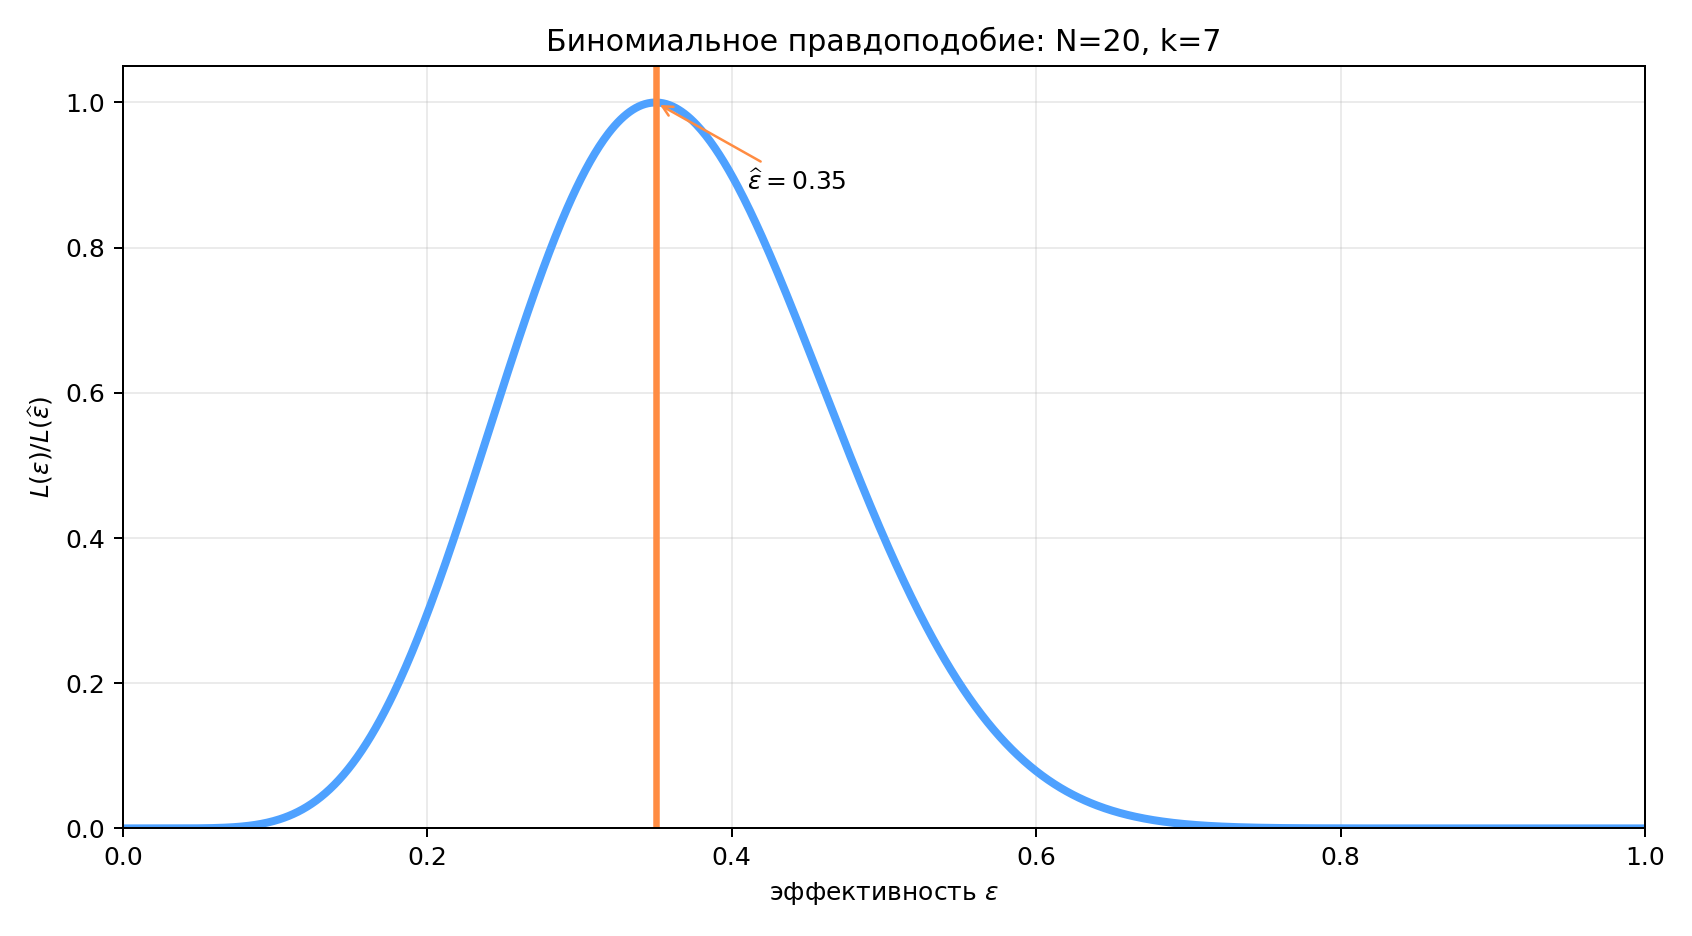
\includegraphics[width=0.74\linewidth,height=\textheight,keepaspectratio,alt={Биномиальное правдоподобие}]{assets/figures/mle_binomial_n20_k7.png}

\end{center}

\noindent\begin{minipage}[c]{\dimexpr\linewidth-30mm\relax}

\textbf{Интерактив}. \textbf{Биномиальное правдоподобие}

Меняйте число частиц \(N\) и число срабатываний \(k\). Вертикальная
линия показывает оценку \(\widehat\varepsilon=k/N\). При увеличении
выборки максимум становится уже.

\end{minipage}\hfill\begin{minipage}[c]{26mm}\centering

\href{https://neutrinohit.github.io/statistical-analysis-course/ru/book/chapters/09_maximum_likelihood.html\#interactive-likelihood-binomial}{
\includegraphics[width=24mm,height=\textheight,keepaspectratio,alt={QR-код интерактива}]{assets/qr/likelihood-binomial.png}}

\end{minipage}

\end{semanticpdfbox}

На рисунке \ref{fig-ch9-binomial-likelihood-large-sample} отношение
\(k/N\) сохранено, но число испытаний увеличено в пять раз. Положение
максимума не изменилось, а значения эффективности вдали от \(0.35\)
теперь подавлены гораздо сильнее.

\begin{figure}

\centering{

\pandocbounded{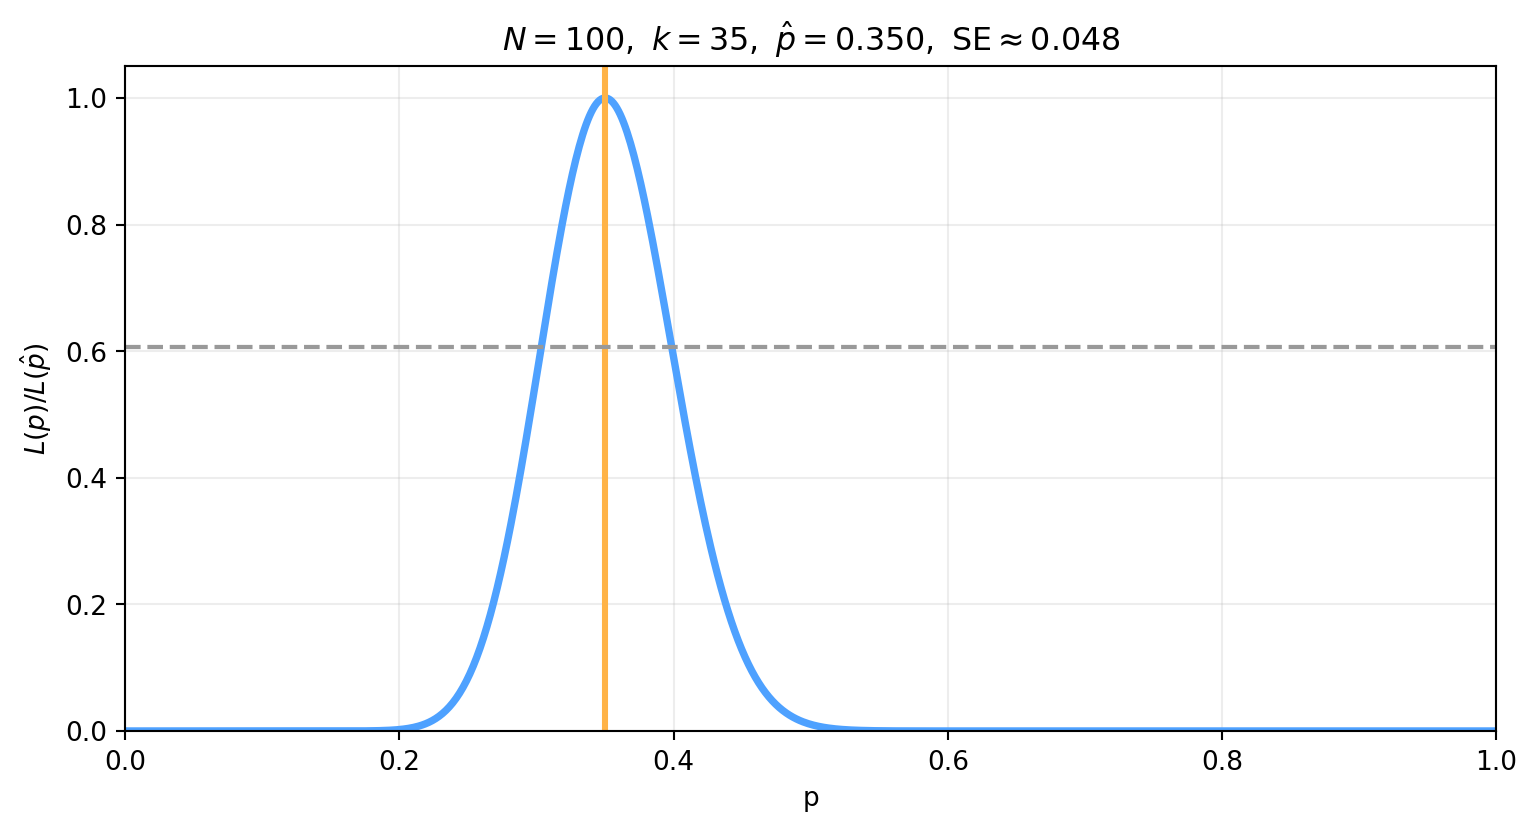
\includegraphics[keepaspectratio]{chapters/../assets/figures/mle_binomial_n100_k35.png}}

}

\caption{\label{fig-ch9-binomial-likelihood-large-sample}Относительное
правдоподобие эффективности при \(N=100\) и \(k=35\). Вертикальная линия
соответствует \(\widehat\varepsilon=0.35\).}

\end{figure}%

Биномиальная модель предполагает, что каждая отмеченная первым прибором
частица действительно прошла через исследуемый детектор, а вероятность
его срабатывания оставалась постоянной. Фоновые совпадения, зависимость
эффективности от энергии и неоднородность детектора добавят в
правдоподобие новые параметры. Одна дробь \(k/N\) такую калибровку уже
не описывает.

\section{Пуассоновский
счёт}\label{ux43fux443ux430ux441ux441ux43eux43dux43eux432ux441ux43aux438ux439-ux441ux447ux451ux442}

Пусть \(N\) --- число событий, зарегистрированных за фиксированное
время, а \(\mu\) --- ожидаемое число событий:

\begin{equation}\protect\phantomsection\label{eq-ch9-poisson-model}{
N\sim\operatorname{Pois}(\mu).
}\end{equation}

Если получено \(n\) событий, правдоподобие равно

\begin{equation}\protect\phantomsection\label{eq-ch9-poisson-likelihood}{
L(\mu)=\frac{\mu^n e^{-\mu}}{n!},
\qquad \mu\geq0.
}\end{equation}

Для \(n>0\)

\begin{equation}\protect\phantomsection\label{eq-ch9-poisson-log-likelihood}{
\ell(\mu)=n\ln\mu-\mu-\ln n!,
\qquad
\frac{d\ell}{d\mu}=\frac n\mu-1.
}\end{equation}

Следовательно,

\begin{equation}\protect\phantomsection\label{eq-ch9-poisson-mle}{
\boxed{\widehat\mu_{\mathrm{ММП}}=n}.
}\end{equation}

При \(n=0\) максимум находится на границе \(\mu=0\), и ответ остаётся
тем же. Поскольку до эксперимента \(\widehat\mu=N\), а
\(\mathbb E[N]=\mu\), эта оценка несмещённая.

\subsection{Известный
фон}\label{ux438ux437ux432ux435ux441ux442ux43dux44bux439-ux444ux43eux43d}

Теперь пусть среднее число событий складывается из неизвестного сигнала
\(s\) и известного фона \(b\):

\begin{equation}\protect\phantomsection\label{eq-ch9-signal-background-model}{
N\sim\operatorname{Pois}(s+b),
\qquad s\geq0.
}\end{equation}

Если временно разрешить \(s\) принимать любые значения при условии
\(s+b\geq0\), максимум находится при

\begin{equation}\protect\phantomsection\label{eq-ch9-unconstrained-signal-mle}{
\widehat s_{\mathrm{unconstrained}}=n-b.
}\end{equation}

Однако отрицательное среднее число сигнальных событий не имеет
физического смысла. С учётом ограничения \(s\geq0\) получаем

\begin{equation}\protect\phantomsection\label{eq-ch9-constrained-signal-mle}{
\boxed{
\widehat s_{\mathrm{ММП}}=\max(0,n-b)
}.
}\end{equation}

При \(n<b\) производная логарифма правдоподобия в разрешённой области не
обращается в нуль. Максимум находится в точке \(s=0\). Физическая
граница меняет статистическую процедуру, и обычное гауссово приближение
возле максимума в этой ситуации требует отдельной проверки.

\section{Среднее гауссова
распределения}\label{ux441ux440ux435ux434ux43dux435ux435-ux433ux430ux443ux441ux441ux43eux432ux430-ux440ux430ux441ux43fux440ux435ux434ux435ux43bux435ux43dux438ux44f}

Пусть независимые измерения имеют одинаковую известную ошибку
\(\sigma\):

\begin{equation}\protect\phantomsection\label{eq-ch9-gaussian-model-known-variance}{
X_i\sim\mathrm N(\mu,\sigma^2),
\qquad i=1,\ldots,N.
}\end{equation}

Требуется оценить \(\mu\). Логарифм правдоподобия с точностью до
постоянного слагаемого равен

\begin{equation}\protect\phantomsection\label{eq-ch9-gaussian-mean-log-likelihood}{
\ell(\mu)
=-\frac{1}{2\sigma^2}
\sum_{i=1}^{N}(x_i-\mu)^2+\mathrm{const}.
}\end{equation}

Максимизация \(\ell\) совпадает с минимизацией суммы квадратов
отклонений. Из условия

\begin{equation}\protect\phantomsection\label{eq-ch9-gaussian-mean-score}{
\frac{d\ell}{d\mu}
=\frac1{\sigma^2}\sum_{i=1}^{N}(x_i-\mu)=0
}\end{equation}

получаем

\begin{equation}\protect\phantomsection\label{eq-ch9-gaussian-mean-mle}{
\boxed{
\widehat\mu_{\mathrm{ММП}}
=\frac1N\sum_{i=1}^{N}x_i
=\overline x
}.
}\end{equation}

Метод максимального правдоподобия выбрал из трёх оценок
\ref{eq-ch9-three-estimators} выборочное среднее. Связь между гауссовым
правдоподобием и методом наименьших квадратов будет подробно
использована в следующих главах.

Если ошибки отдельных измерений \(\sigma_i\) различаются, в сумме
появляется вес \(1/\sigma_i^2\). Максимум правдоподобия тогда даёт
взвешенное среднее, полученное в формуле
\ref{eq-ch7-independent-weighted-mean}.

\section{Неизвестны среднее и
дисперсия}\label{ux43dux435ux438ux437ux432ux435ux441ux442ux43dux44b-ux441ux440ux435ux434ux43dux435ux435-ux438-ux434ux438ux441ux43fux435ux440ux441ux438ux44f}

Пусть теперь требуется одновременно оценить \(\mu\) и \(\sigma^2\).
Полный логарифм правдоподобия имеет вид

\begin{equation}\protect\phantomsection\label{eq-ch9-gaussian-two-parameter-log-likelihood}{
\ell(\mu,\sigma^2)
=-\frac N2\ln(2\pi\sigma^2)
-\frac1{2\sigma^2}
\sum_{i=1}^{N}(x_i-\mu)^2.
}\end{equation}

Нормировочный множитель гауссова распределения теперь зависит от
\(\sigma^2\), поэтому отбрасывать первое слагаемое нельзя. Максимизация
по двум параметрам даёт

\begin{equation}\protect\phantomsection\label{eq-ch9-gaussian-mean-variance-mle}{
\boxed{
\widehat\mu_{\mathrm{ММП}}=\overline x,
\qquad
\widehat{\sigma^2}_{\mathrm{ММП}}
=\frac1N\sum_{i=1}^{N}(x_i-\overline x)^2
}.
}\end{equation}

Оценка среднего несмещённая. Для дисперсии получается другой результат:

\begin{equation}\protect\phantomsection\label{eq-ch9-gaussian-variance-mle-bias}{
\mathbb E\!\left[
\widehat{\sigma^2}_{\mathrm{ММП}}
\right]
=\frac{N-1}{N}\sigma^2.
}\end{equation}

Делитель \(N\) появился из условия максимума правдоподобия. Несмещённая
оценка дисперсии использует делитель \(N-1\):

\begin{equation}\protect\phantomsection\label{eq-ch9-unbiased-sample-variance}{
s^2
=\frac1{N-1}\sum_{i=1}^{N}(x_i-\overline x)^2,
\qquad
\mathbb E[s^2]=\sigma^2.
}\end{equation}

Здесь оценка максимального правдоподобия и несмещённая оценка
расходятся. Метод максимального правдоподобия задаёт способ построения
оценки. Несмещённость --- отдельное свойство этой оценки. Для
\(\widehat{\sigma^2}_{\mathrm{ММП}}\) смещение исчезает при
\(N\to\infty\), но при конечном \(N\) оно существует.

\section{Что уже можно прочитать по функции
правдоподобия}\label{ux447ux442ux43e-ux443ux436ux435-ux43cux43eux436ux43dux43e-ux43fux440ux43eux447ux438ux442ux430ux442ux44c-ux43fux43e-ux444ux443ux43dux43aux446ux438ux438-ux43fux440ux430ux432ux434ux43eux43fux43eux434ux43eux431ux438ux44f}

Положение максимума даёт точечную оценку. Ширина максимума показывает,
как быстро ухудшается согласие модели с данными при смещении параметра.
С ростом выборки максимум обычно сужается, как в биномиальном примере.
Если максимум прижат к границе, форма функции становится несимметричной.

Эти наблюдения пока остаются качественными. Чтобы превратить ширину
правдоподобия в ошибку оценки или интервал, потребуется определить
статистическую процедуру и проверить её свойства. Этому посвящена
следующая глава.

\begin{bookchaptersummary}[Итоги главы]

\begin{itemize}
\tightlist
\item
  Оценка является функцией случайных данных; после подстановки выборки
  она принимает конкретное значение.
\item
  Правдоподобие сравнивает значения параметров при фиксированных данных
  и не является распределением вероятности параметра.
\item
  Для независимых измерений правдоподобия перемножаются, а их логарифмы
  складываются.
\item
  Оценка максимального правдоподобия соответствует максимуму \(L\) в
  допустимой области параметров.
\item
  Метод максимального правдоподобия не гарантирует несмещённость: для
  гауссовой дисперсии оценка с делителем \(N\) смещена при конечной
  выборке.
\end{itemize}

\end{bookchaptersummary}

\section{Задачи}\label{ux437ux430ux434ux430ux447ux438-8}

\begin{semanticpdfbox}[colback=BookCoralSoft,borderline west={1.2mm}{0pt}{BookCoral},breakable=false]

\noindent{\sffamily\bfseries\fontsize{11.2}{13.5}\selectfont Задача 1. Вероятность и правдоподобие}\par\nopagebreak[4]\vspace{1.2mm}

Одно наблюдение \(x\) получено из экспоненциального распределения \[
f(x\mid\lambda)=\lambda e^{-\lambda x},
\qquad x\ge0.
\]

\begin{enumerate}
\def\labelenumi{\arabic{enumi}.}
\tightlist
\item
  Нарисуйте \(f(x\mid\lambda)\) как функцию \(x\) при нескольких
  фиксированных \(\lambda\).
\item
  После наблюдения \(x=x_{\mathrm{obs}}\) запишите
  \(L(\lambda;x_{\mathrm{obs}})\).
\item
  Вычислите \(\int_0^\infty L(\lambda;x_{\mathrm{obs}})\,d\lambda\).
  Почему этот интеграл не является условием нормировки вероятности
  параметра?
\item
  Найдите \(\widehat\lambda_{\mathrm{ММП}}\).
\item
  Объясните словами различие между плотностью вероятности и функцией
  правдоподобия.
\end{enumerate}

\end{semanticpdfbox}

\begin{semanticpdfbox}[colback=BookCoralSoft,borderline west={1.2mm}{0pt}{BookCoral},breakable=false]

\noindent{\sffamily\bfseries\fontsize{11.2}{13.5}\selectfont Задача 2. Биномиальная оценка}\par\nopagebreak[4]\vspace{1.2mm}

В \(N\) независимых испытаниях наблюдалось \(k\) успехов.

\begin{enumerate}
\def\labelenumi{\arabic{enumi}.}
\tightlist
\item
  Запишите биномиальное правдоподобие \(L(p)\).
\item
  Найдите \(\widehat p_{\mathrm{ММП}}\).
\item
  Вычислите \(\mathbb E[\widehat p]\) и
  \(\operatorname{Var}(\widehat p)\).
\item
  Покажите, что оценка несмещённая и состоятельная.
\item
  Исследуйте форму \(L(p)\) для случаев \(k=0\), \(k=N/2\) и \(k=N\).
\end{enumerate}

\end{semanticpdfbox}

\begin{semanticpdfbox}[colback=BookCoralSoft,borderline west={1.2mm}{0pt}{BookCoral},breakable=false]

\noindent{\sffamily\bfseries\fontsize{11.2}{13.5}\selectfont Задача 3. Пуассоновский счёт с известным фоном}\par\nopagebreak[4]\vspace{1.2mm}

Пусть \[
N\sim\operatorname{Pois}(s+b),
\] где \(s\ge0\) --- неизвестный сигнал, а фон \(b\) известен точно.

\begin{enumerate}
\def\labelenumi{\arabic{enumi}.}
\tightlist
\item
  Запишите \(L(s)\) и \(\ell(s)\).
\item
  Найдите неограниченную оценку максимального правдоподобия сигнала.
\item
  Найдите оценку максимального правдоподобия при физическом ограничении
  \(s\ge0\).
\item
  Объясните, что происходит при \(n<b\).
\end{enumerate}

\end{semanticpdfbox}

\begin{semanticpdfbox}[colback=BookCoralSoft,borderline west={1.2mm}{0pt}{BookCoral},breakable=false]

\noindent{\sffamily\bfseries\fontsize{11.2}{13.5}\selectfont Задача 4. Гауссово среднее}\par\nopagebreak[4]\vspace{1.2mm}

Пусть \[
X_i\sim\mathrm N(\mu,\sigma^2),
\] где \(\sigma\) известна.

\begin{enumerate}
\def\labelenumi{\arabic{enumi}.}
\tightlist
\item
  Запишите функцию правдоподобия независимой выборки.
\item
  Покажите, что \(\widehat\mu_{\mathrm{ММП}}=\langle X\rangle\).
\item
  Найдите \(\operatorname{Var}(\widehat\mu_{\mathrm{ММП}})\).
\end{enumerate}

\end{semanticpdfbox}

\begin{semanticpdfbox}[colback=BookCoralSoft,borderline west={1.2mm}{0pt}{BookCoral},breakable=false]

\noindent{\sffamily\bfseries\fontsize{11.2}{13.5}\selectfont Задача 5. Взвешенное среднее}\par\nopagebreak[4]\vspace{1.2mm}

Имеются независимые измерения \[
X_i\sim\mathrm N(\mu,\sigma_i^2),
\] где \(\sigma_i\) известны и различаются.

\begin{enumerate}
\def\labelenumi{\arabic{enumi}.}
\tightlist
\item
  Запишите совместный логарифм функции правдоподобия.
\item
  Найдите оценку максимального правдоподобия параметра \(\mu\).
\item
  Покажите, что результат является взвешенным средним с весами
  \(w_i=1/\sigma_i^2\).
\item
  Найдите дисперсию оценки.
\item
  Объясните, почему измерения с меньшей ошибкой получают больший вес.
\end{enumerate}

\end{semanticpdfbox}

\section*{Литература}\label{ux43bux438ux442ux435ux440ux430ux442ux443ux440ux430-8}
\addcontentsline{toc}{section}{Литература}

\markright{Литература}

\protect\phantomsection\label{refs}
\begin{CSLReferences}{0}{0}
\bibitem[\citeproctext]{ref-fisher1922}
{[}1{]} Fisher, R. A. On the Mathematical Foundations of Theoretical
Statistics. \emph{Philosophical Transactions of the Royal Society of
London. Series A}, \textbf{222}, 309--368. 1922.
doi:\href{https://doi.org/10.1098/rsta.1922.0009}{10.1098/rsta.1922.0009}.

\bibitem[\citeproctext]{ref-cowan1998}
{[}2{]} Cowan, G. \emph{Statistical Data Analysis}. Oxford University
Press. 1998.

\end{CSLReferences}

\chapter{Свойства оценок и профильное
правдоподобие}\label{ux441ux432ux43eux439ux441ux442ux432ux430-ux43eux446ux435ux43dux43eux43a-ux438-ux43fux440ux43eux444ux438ux43bux44cux43dux43eux435-ux43fux440ux430ux432ux434ux43eux43fux43eux434ux43eux431ux438ux435}

\bookchapteropeningcontents

\begin{bookchapteropening}[Аннотация]

В прошлой главе мы научились находить максимум правдоподобия. Теперь
разберём, какими свойствами обладает полученная оценка и как определить
её ошибку. Для этого введём смещение, средний квадрат ошибки и
информацию Фишера, исследуем форму правдоподобия и научимся учитывать
мешающие параметры. Примерами послужат измерение времени жизни частицы и
подгонка спектра реакторных антинейтрино.

\end{bookchapteropening}

\section{Физическая задача: время жизни
частицы}\label{ux444ux438ux437ux438ux447ux435ux441ux43aux430ux44f-ux437ux430ux434ux430ux447ux430-ux432ux440ux435ux43cux44f-ux436ux438ux437ux43dux438-ux447ux430ux441ux442ux438ux446ux44b}

Детектор зарегистрировал \(N=20\) распадов. Для каждого события измерено
время от рождения частицы до её распада. Сумма этих времён оказалась
равна \(40\ \text{мкс}\). Как оценить среднее время жизни \(\tau\)?

В простейшей модели времена независимы и имеют экспоненциальное
распределение. Фоном, разрешением прибора и потерями событий
пренебрежём. Предполагается, что регистрация одинаково эффективна при
любом времени распада. Тогда оценка максимального правдоподобия равна
среднему по выборке:

\begin{equation}\protect\phantomsection\label{eq-ch10-lifetime-first-estimate}{
\widehat\tau=\frac1N\sum_{i=1}^{N}t_i
=2.0\ \text{мкс}.
}\end{equation}

А какая у неё ошибка? Если использовать свойства экспоненциального
распределения, стандартное отклонение оценки получится равным
\(\tau/\sqrt N\). Истинного \(\tau\) мы пока не знаем. Подставляя вместо
него оценку, получим

\begin{equation}\protect\phantomsection\label{eq-ch10-lifetime-first-error}{
\widehat\sigma_{\widehat\tau}
=\frac{\widehat\tau}{\sqrt N}
\simeq0.45\ \text{мкс}.
}\end{equation}

Двадцать событий дали нам время жизни с относительной статистической
ошибкой около \(22\%\). Можно ли при том же числе событий придумать
оценку поточнее? Насколько обоснована симметричная запись
\(2.0\pm0.45\ \text{мкс}\)? И что изменится, когда в модели появится
неизвестный фон?

Для ответа надо посмотреть, как оценка ведёт себя при повторении
эксперимента. Все ожидания и дисперсии ниже относятся к ансамблю
возможных данных при фиксированном истинном параметре.

\section{Свойства
оценок}\label{ux441ux432ux43eux439ux441ux442ux432ux430-ux43eux446ux435ux43dux43eux43a}

\subsection{Смещение, дисперсия и средний квадрат
ошибки}\label{ux441ux43cux435ux449ux435ux43dux438ux435-ux434ux438ux441ux43fux435ux440ux441ux438ux44f-ux438-ux441ux440ux435ux434ux43dux438ux439-ux43aux432ux430ux434ux440ux430ux442-ux43eux448ux438ux431ux43aux438}

Пусть мы много раз повторили один и тот же эксперимент и каждый раз
получили оценку \(\widehat\theta\). Среднее этих оценок может отличаться
от истинного значения \(\theta\). Разность называется
\textbf{смещением}:

\begin{equation}\protect\phantomsection\label{eq-ch10-estimator-bias}{
b(\theta)=\operatorname{bias}(\widehat\theta)
=\mathbb E_\theta[\widehat\theta]-\theta.
}\end{equation}

Если \(b(\theta)=0\) для всех допустимых \(\theta\), оценка несмещённая.
Это свойство среднего по ансамблю. Отдельное измерение, конечно, не
обязано попасть в истинное значение. Разброс оценок около их
собственного среднего описывается дисперсией
\(\operatorname{Var}_\theta(\widehat\theta)\).

Чтобы учесть и смещение, и разброс, введём \textbf{средний квадрат
ошибки}, или MSE (\emph{mean squared error}):

\begin{equation}\protect\phantomsection\label{eq-ch10-mse-definition}{
\operatorname{MSE}_\theta(\widehat\theta)
=\mathbb E_\theta[(\widehat\theta-\theta)^2].
}\end{equation}

Здесь отклонение отсчитывается от истинного параметра. Добавим и вычтем
\(m=\mathbb E_\theta[\widehat\theta]\):

\[
\widehat\theta-\theta=(\widehat\theta-m)+(m-\theta).
\]

После возведения в квадрат смешанный член исчезает при усреднении,
поскольку \(\mathbb E_\theta[\widehat\theta-m]=0\). Остаётся

\begin{equation}\protect\phantomsection\label{eq-ch10-mse-decomposition}{
\boxed{
\operatorname{MSE}_\theta(\widehat\theta)
=\operatorname{Var}_\theta(\widehat\theta)+b^2(\theta).
}
}\end{equation}

Получается, что устранение смещения само по себе ещё не гарантирует
меньшей ошибки. Посмотрим на пример, который уже встретился нам в
прошлой главе.

\subsection{Два делителя в оценке
дисперсии}\label{interactive-likelihood-variance-estimators}

Для независимой гауссовой выборки размера \(N\geq2\) с неизвестными
\(\mu\) и \(\sigma^2\) имеем две оценки:

\begin{equation}\protect\phantomsection\label{eq-ch10-two-variance-estimators}{
\widehat{\sigma^2}_{\mathrm{ММП}}
=\frac1N\sum_{i=1}^{N}(X_i-\overline X)^2,
\qquad
s^2=\frac1{N-1}\sum_{i=1}^{N}(X_i-\overline X)^2.
}\end{equation}

Первая получается максимизацией правдоподобия. Вторая несмещённая. Их
средние равны

\begin{equation}\protect\phantomsection\label{eq-ch10-variance-estimator-means}{
\mathbb E[\widehat{\sigma^2}_{\mathrm{ММП}}]
=\frac{N-1}{N}\sigma^2,
\qquad
\mathbb E[s^2]=\sigma^2.
}\end{equation}

Но у \(s^2\) больше разброс: каждый результат первой оценки умножен на
\(N/(N-1)\). Для гауссовой выборки точный расчёт даёт

\begin{equation}\protect\phantomsection\label{eq-ch10-variance-estimator-variances}{
\operatorname{Var}(\widehat{\sigma^2}_{\mathrm{ММП}})
=\frac{2(N-1)}{N^2}\sigma^4,
\qquad
\operatorname{Var}(s^2)=\frac{2}{N-1}\sigma^4.
}\end{equation}

Подставим эти выражения в формулу \ref{eq-ch10-mse-decomposition}:

\begin{equation}\protect\phantomsection\label{eq-ch10-variance-estimator-mse}{
\operatorname{MSE}(\widehat{\sigma^2}_{\mathrm{ММП}})
=\frac{2N-1}{N^2}\sigma^4,
\qquad
\operatorname{MSE}(s^2)=\frac{2}{N-1}\sigma^4.
}\end{equation}

При \(N=6\) коэффициенты перед \(\sigma^4\) равны примерно \(0.306\) и
\(0.400\). Смещённая оценка в этом сравнении выигрывает по среднему
квадрату ошибки. Это не делает её лучшей для любой задачи: мы выбрали
конкретный критерий и посчитали его в конкретной модели.

В апплете истинная дисперсия равна единице. Для каждой из \(6000\)
гауссовых выборок вычисляются обе оценки. Сравните положения гистограмм,
их ширины и средние квадраты ошибок. Затем увеличьте \(N\).

\begin{semanticpdfbox}[breakable=false]

\begin{center}

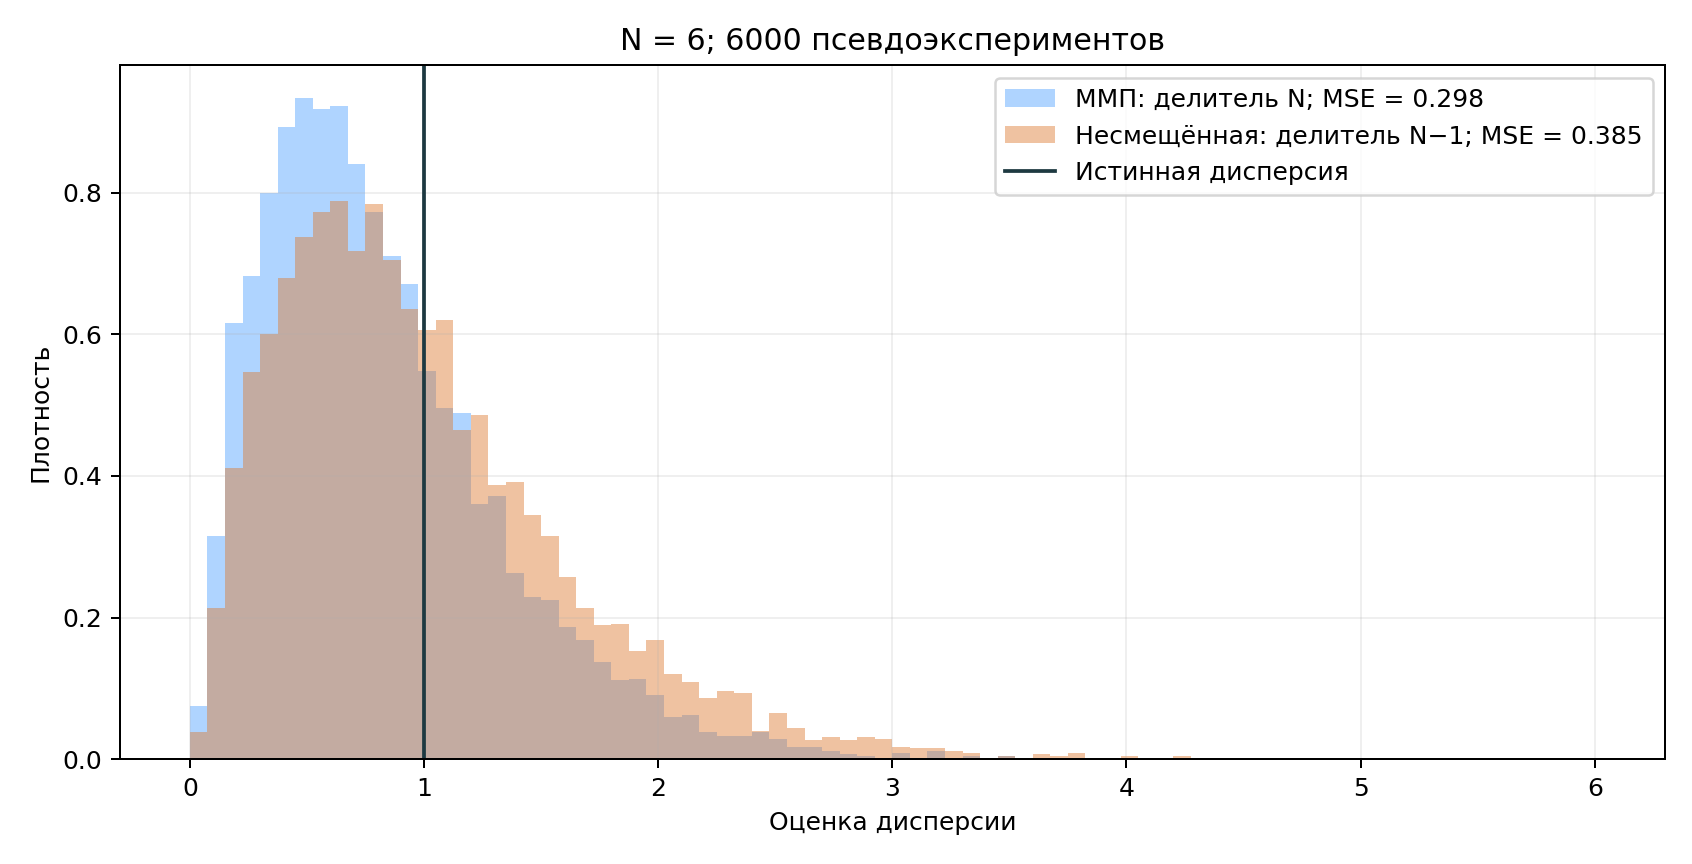
\includegraphics[width=0.74\linewidth,height=\textheight,keepaspectratio,alt={Две оценки дисперсии}]{assets/figures/mle_variance_estimators_n6.png}

\end{center}

\noindent\begin{minipage}[c]{\dimexpr\linewidth-30mm\relax}

\textbf{Интерактив}. \textbf{Две оценки дисперсии}

Распределения оценок дисперсии для \(6000\) гауссовых выборок размера
\(N=6\) при \(\sigma^2=1\). Делитель \(N-1\) устраняет смещение и
одновременно увеличивает разброс оценки.

\end{minipage}\hfill\begin{minipage}[c]{26mm}\centering

\href{https://neutrinohit.github.io/statistical-analysis-course/ru/book/chapters/10_estimator_properties_profile_likelihood.html\#interactive-likelihood-variance-estimators}{
\includegraphics[width=24mm,height=\textheight,keepaspectratio,alt={QR-код интерактива}]{assets/qr/likelihood-variance-estimators.png}}

\end{minipage}

\end{semanticpdfbox}

\subsection{Состоятельность}\label{ux441ux43eux441ux442ux43eux44fux442ux435ux43bux44cux43dux43eux441ux442ux44c}

Что должно происходить с оценкой, когда данных становится всё больше? Мы
хотим, чтобы вероятность заметно промахнуться мимо истинного параметра
стремилась к нулю. Это свойство называется \textbf{состоятельностью}:

\begin{equation}\protect\phantomsection\label{eq-ch10-consistency}{
P_\theta\!\left(|\widehat\theta_N-\theta|>\varepsilon\right)
\xrightarrow[N\to\infty]{}0
\quad\text{при любом }\varepsilon>0.
}\end{equation}

Короткая запись этого условия ---
\(\widehat\theta_N\xrightarrow{P}\theta\). Например, закон больших чисел
обеспечивает состоятельность выборочного среднего при существующем
конечном математическом ожидании.

Удобный достаточный признак состоятельности --- одновременно исчезающие
смещение и дисперсия. Действительно,

\begin{equation}\protect\phantomsection\label{eq-ch10-consistency-mse-bound}{
P_\theta\!\left(|\widehat\theta_N-\theta|>\varepsilon\right)
\leq
\frac{\operatorname{MSE}_\theta(\widehat\theta_N)}{\varepsilon^2}.
}\end{equation}

Если правая часть стремится к нулю, выполнено определение
\ref{eq-ch10-consistency}. Обратного вывода без дополнительных условий
нет: редкие, но очень большие отклонения могут мешать сходимости
моментов.

\subsection{Сравнение трёх оценок гауссова
среднего}\label{ux441ux440ux430ux432ux43dux435ux43dux438ux435-ux442ux440ux451ux445-ux43eux446ux435ux43dux43eux43a-ux433ux430ux443ux441ux441ux43eux432ux430-ux441ux440ux435ux434ux43dux435ux433ux43e}

В прошлой главе мы предложили три правила оценки \(\mu\): среднее по
всей выборке, медиану и полусумму первого и последнего измерений. Для
независимых \(X_i\sim\mathcal N(\mu,\sigma^2)\) получаем

\begin{equation}\protect\phantomsection\label{eq-ch10-three-estimator-variances}{
\begin{aligned}
\operatorname{Var}(\overline X)&=\frac{\sigma^2}{N},\\
\operatorname{Var}(\operatorname{median}X_i)
&\simeq\frac{\pi}{2}\frac{\sigma^2}{N},\\
\operatorname{Var}\!\left(\frac{X_1+X_N}{2}\right)
&=\frac{\sigma^2}{2},\qquad N\geq2.
\end{aligned}
}\end{equation}

Первая и третья формулы точные; формула для медианы асимптотическая, при
большом \(N\). Среднее и медиана состоятельны. У третьей оценки
распределение вообще не меняется при добавлении данных: два
использованных измерения остаются двумя измерениями. Несмещённость здесь
есть, состоятельности нет.

В чистой гауссовой модели среднее точнее медианы. Зато медиана слабее
реагирует на отдельные выбросы. Если в данные попадают события из
другого процесса, сначала надо разобраться с моделью выборки. Вывод об
оптимальности среднего был получен для гауссовой модели без такой
примеси.

\section{Информация Фишера и граница
Крамера--Рао}\label{ux438ux43dux444ux43eux440ux43cux430ux446ux438ux44f-ux444ux438ux448ux435ux440ux430-ux438-ux433ux440ux430ux43dux438ux446ux430-ux43aux440ux430ux43cux435ux440ux430ux440ux430ux43e}

Можно ли найти нижнюю границу дисперсии оценки, ещё не выбрав саму
оценку? В регулярных моделях это позволяет сделать информация Фишера
{[}1{]}.

Обозначим логарифм правдоподобия всей выборки через \(\ell(\theta)\) и
введём его производную --- \textbf{скор-функцию} (\emph{score}):

\begin{equation}\protect\phantomsection\label{eq-ch10-score}{
U(\theta)=\frac{\partial\ell(\theta)}{\partial\theta}.
}\end{equation}

До подстановки данных \(U(\theta)\) является случайной величиной. Для
информации Фишера существуют две равносильные записи:

\begin{equation}\protect\phantomsection\label{eq-fisher-information}{
\boxed{
I(\theta)=\mathbb E_\theta[U^2(\theta)]
=-\mathbb E_\theta\!\left[
\frac{\partial^2\ell(\theta)}{\partial\theta^2}\right].
}
}\end{equation}

В каких условиях они равносильны? Область возможных данных не должна
зависеть от параметра; плотность должна быть достаточно гладкой, чтобы
производные можно было переносить под интеграл. В дальнейшем также
предполагаем \(0<I(\theta)<\infty\). Посмотрим, где используются эти
условия.

\subsection{Две формы информации
Фишера}\label{ux434ux432ux435-ux444ux43eux440ux43cux44b-ux438ux43dux444ux43eux440ux43cux430ux446ux438ux438-ux444ux438ux448ux435ux440ux430}

Для одного наблюдения положим \(u=\partial_\theta\ln f(x\mid\theta)\).
Дифференцируя условие нормировки, получаем

\begin{equation}\protect\phantomsection\label{eq-ch10-score-zero-mean}{
0=\frac{\partial}{\partial\theta}\int f(x\mid\theta)\,dx
=\int f(x\mid\theta)u\,dx
=\mathbb E_\theta[u].
}\end{equation}

Ещё одно дифференцирование даёт

\[
\begin{aligned}
0&=\int\frac{\partial^2f}{\partial\theta^2}\,dx\\
&=\int f\left[u^2+\frac{\partial^2\ln f}{\partial\theta^2}\right]dx.
\end{aligned}
\]

Отсюда следует формула \ref{eq-fisher-information} для одного
наблюдения. Для независимых наблюдений логарифмы правдоподобия и их
производные складываются. Средние скор-функций равны нулю, поэтому
смешанные члены в квадрате суммы исчезают:

\begin{equation}\protect\phantomsection\label{eq-ch10-information-additivity}{
I_N(\theta)=\sum_{i=1}^{N}I_i(\theta).
}\end{equation}

Для одинаково распределённых наблюдений \(I_N=NI_1\). Это и есть
количественная мера того, как растёт информация при накоплении
статистики.

\subsection{Граница
Крамера--Рао}\label{ux433ux440ux430ux43dux438ux446ux430-ux43aux440ux430ux43cux435ux440ux430ux440ux430ux43e}

Для несмещённой оценки \(T(\mathbf X)\) дифференцируем равенство
\(\mathbb E_\theta[T]=\theta\). Если производную снова можно перенести
под интеграл, получаем

\[
1=\mathbb E_\theta[TU]
=\mathbb E_\theta[(T-\theta)U].
\]

По неравенству Коши--Буняковского квадрат среднего произведения не
больше произведения средних квадратов. Следовательно,

\begin{equation}\protect\phantomsection\label{eq-ch10-cramer-rao-bound}{
1\leq\operatorname{Var}_\theta(T)\,I(\theta),
\qquad
\boxed{\operatorname{Var}_\theta(T)\geq\frac1{I(\theta)}.}
}\end{equation}

Это \textbf{граница Крамера--Рао}. Несмещённую оценку, достигающую
границы, называют эффективной. Достижимость не гарантируется для
произвольной модели. Смещённые оценки также не обязаны подчиняться
границе именно в таком виде: в её выводе мы использовали
\(\mathbb E_\theta[T]=\theta\).

\subsection{Пример: гауссово
среднее}\label{ux43fux440ux438ux43cux435ux440-ux433ux430ux443ux441ux441ux43eux432ux43e-ux441ux440ux435ux434ux43dux435ux435}

Для одного гауссова измерения с известной \(\sigma\) скор-функция равна

\begin{equation}\protect\phantomsection\label{eq-ch10-gaussian-information}{
u_\mu(X)=\frac{X-\mu}{\sigma^2},
\qquad
I_1(\mu)=\frac{\mathbb E[(X-\mu)^2]}{\sigma^4}
=\frac1{\sigma^2}.
}\end{equation}

Для \(N\) независимых измерений \(I_N=N/\sigma^2\). Значит, дисперсия
любой несмещённой оценки \(\mu\) не меньше \(\sigma^2/N\). Выборочное
среднее имеет ровно эту дисперсию. В принятой модели мы уже получили
эффективную оценку.

\section{Форма правдоподобия около
максимума}\label{ux444ux43eux440ux43cux430-ux43fux440ux430ux432ux434ux43eux43fux43eux434ux43eux431ux438ux44f-ux43eux43aux43eux43bux43e-ux43cux430ux43aux441ux438ux43cux443ux43cux430}

Информация Фишера содержит усреднение по возможным данным. После
эксперимента мы располагаем одной выборкой и одной функцией
\(\ell(\theta)\). Её кривизну можно вычислить непосредственно.

Пусть максимум находится внутри допустимой области, а \(\ell\) гладкая.
Разложим её около \(\widehat\theta\). Первая производная в максимуме
равна нулю:

\begin{equation}\protect\phantomsection\label{eq-ch10-likelihood-taylor}{
\ell(\theta)\simeq\ell(\widehat\theta)
-\frac12J(\widehat\theta)(\theta-\widehat\theta)^2,
\qquad
J(\widehat\theta)=-\ell''(\widehat\theta).
}\end{equation}

Величина \(J(\widehat\theta)\) определяется конкретной выборкой. При
регулярной модели и достаточно большом \(N\) обратная кривизна даёт
оценку дисперсии ММП:

\begin{equation}\protect\phantomsection\label{eq-ch10-curvature-error}{
\widehat\sigma_{\widehat\theta}^{\,2}
\simeq\frac1{J(\widehat\theta)}.
}\end{equation}

Узкий максимум соответствует малой ошибке. Но само наличие максимума ещё
не означает, что он хорошо описывается параболой. Асимметрию, границы и
другие максимумы надо проверять по всей функции правдоподобия.

\subsection{Отношение
правдоподобий}\label{ux43eux442ux43dux43eux448ux435ux43dux438ux435-ux43fux440ux430ux432ux434ux43eux43fux43eux434ux43eux431ux438ux439}

Разделим \(L(\theta)\) на его максимальное значение:

\begin{equation}\protect\phantomsection\label{eq-ch10-relative-likelihood}{
\lambda(\theta)=\frac{L(\theta)}{L(\widehat\theta)}.
}\end{equation}

Теперь нормировка сократилась, а максимум равен единице. Для вычислений
удобнее пользоваться логарифмом:

\begin{equation}\protect\phantomsection\label{eq-likelihood-ratio-statistic}{
\boxed{
q(\theta)=-2\ln\lambda(\theta)
=-2[\ell(\theta)-\ell(\widehat\theta)].
}
}\end{equation}

В максимуме \(q=0\), в остальных точках \(q\geq0\). В квадратичном
приближении

\begin{equation}\protect\phantomsection\label{eq-ch10-quadratic-ratio}{
q(\theta)\simeq
\frac{(\theta-\widehat\theta)^2}
     {\widehat\sigma_{\widehat\theta}^{\,2}}.
}\end{equation}

Поэтому точки \(q=1\) отстоят от оценки на одну стандартную ошибку. На
графике \(\ell\) им соответствует спуск от максимума на \(1/2\).

Для гауссовой выборки с известной \(\sigma\) получаем точное равенство

\begin{equation}\protect\phantomsection\label{eq-ch10-gaussian-ratio}{
q(\mu)=\frac{(\mu-\overline x)^2}{\sigma^2/N}.
}\end{equation}

Здесь интервал \(q(\mu)\leq1\) имеет покрытие около \(68.3\%\): при
повторении эксперимента такая процедура накрывает истинное \(\mu\) с
этой частотой. Для других моделей тот же порог требует обоснования.

Теорема Уилкса даёт его в пределе большой выборки: при истинном значении
одного проверяемого параметра статистика \(q\) асимптотически имеет
распределение \(\chi^2\) с одной степенью свободы {[}2{]}. Нужны
идентифицируемая гладкая модель, невырожденная информация и истинная
точка внутри области параметров. У физической границы или при слабой
чувствительности эти условия могут нарушаться. Частотное покрытие тогда
проверяют отдельно, например на псевдоэкспериментах.

\section{Возвращаемся к времени
жизни}\label{ux432ux43eux437ux432ux440ux430ux449ux430ux435ux43cux441ux44f-ux43a-ux432ux440ux435ux43cux435ux43dux438-ux436ux438ux437ux43dux438}

В нашей модели \(\tau>0\) --- среднее время жизни, а плотность времени
распада равна

\begin{equation}\protect\phantomsection\label{eq-ch10-lifetime-density}{
f(t\mid\tau)=\frac1\tau e^{-t/\tau},\qquad t\geq0.
}\end{equation}

Для \(N\) независимых времён

\begin{equation}\protect\phantomsection\label{eq-ch10-lifetime-likelihood}{
L(\tau)=\tau^{-N}\exp\!\left(-\frac1\tau\sum_i t_i\right),
\qquad
\ell(\tau)=-N\ln\tau-\frac1\tau\sum_i t_i.
}\end{equation}

Как обычно, в логарифме опущена константа, не зависящая от параметра.
Условие максимума имеет вид

\begin{equation}\protect\phantomsection\label{eq-ch10-lifetime-mle}{
\frac{\partial\ell}{\partial\tau}
=-\frac N\tau+\frac{\sum_i t_i}{\tau^2}=0,
\qquad
\widehat\tau=\overline t.
}\end{equation}

Так мы получили формулу, с которой начали главу. У экспоненциальной
величины \(\mathbb E[T_i]=\tau\) и \(\operatorname{Var}(T_i)=\tau^2\),
поэтому

\begin{equation}\protect\phantomsection\label{eq-ch10-lifetime-estimator-moments}{
\mathbb E[\widehat\tau]=\tau,
\qquad
\operatorname{Var}(\widehat\tau)=\frac{\tau^2}{N}.
}\end{equation}

Оценка несмещённая и состоятельная. Информация Фишера равна

\begin{equation}\protect\phantomsection\label{eq-ch10-lifetime-information}{
I_N(\tau)
=-\mathbb E_\tau\!\left[
\frac N{\tau^2}-\frac{2\sum_i T_i}{\tau^3}\right]
=\frac N{\tau^2}.
}\end{equation}

Дисперсия \ref{eq-ch10-lifetime-estimator-moments} достигает границы
Крамера--Рао при любом \(N\). Среди несмещённых оценок сделать её меньше
в этой модели нельзя.

А вот распределение оценки при малом \(N\) ещё не гауссово: сумма
экспоненциальных времён имеет гамма-распределение. Эффективность оценки
и гауссова форма её распределения --- разные свойства. Само
правдоподобие также отличается от гауссова. Для него получаем точное
выражение:

\begin{equation}\protect\phantomsection\label{eq-ch10-lifetime-ratio}{
q(\tau)=2N\left[
\ln\frac\tau{\widehat\tau}+\frac{\widehat\tau}{\tau}-1\right].
}\end{equation}

Оно асимметрично относительно \(\widehat\tau\). Для наших \(N=20\) и
\(\widehat\tau=2.0\ \text{мкс}\) решения уравнения \(q(\tau)=1\) равны
примерно \(1.61\) и \(2.52\ \text{мкс}\). Расстояния до оценки
различаются: \(0.39\) вниз и \(0.52\ \text{мкс}\) вверх. Симметричная
ошибка \(0.45\ \text{мкс}\) передаёт местную кривизну, но теряет эту
асимметрию. Само решение \(q=1\) на конечной выборке ещё не гарантирует
точного покрытия \(68.3\%\).

\subsection{Численный
эксперимент}\label{interactive-likelihood-lifetime}

В апплете генерируются времена распадов при заданном истинном
\(\tau_0\). Двигайте пробное \(\tau\) и найдите максимум. Затем включите
границы \(q=1\). Повторите опыт несколько раз при малом \(N\), а после
увеличьте выборку. Максимум меняется от опыта к опыту; масштаб этого
разброса задаётся формулой \ref{eq-ch10-lifetime-estimator-moments}.

\begin{semanticpdfbox}[breakable=false]

\begin{center}

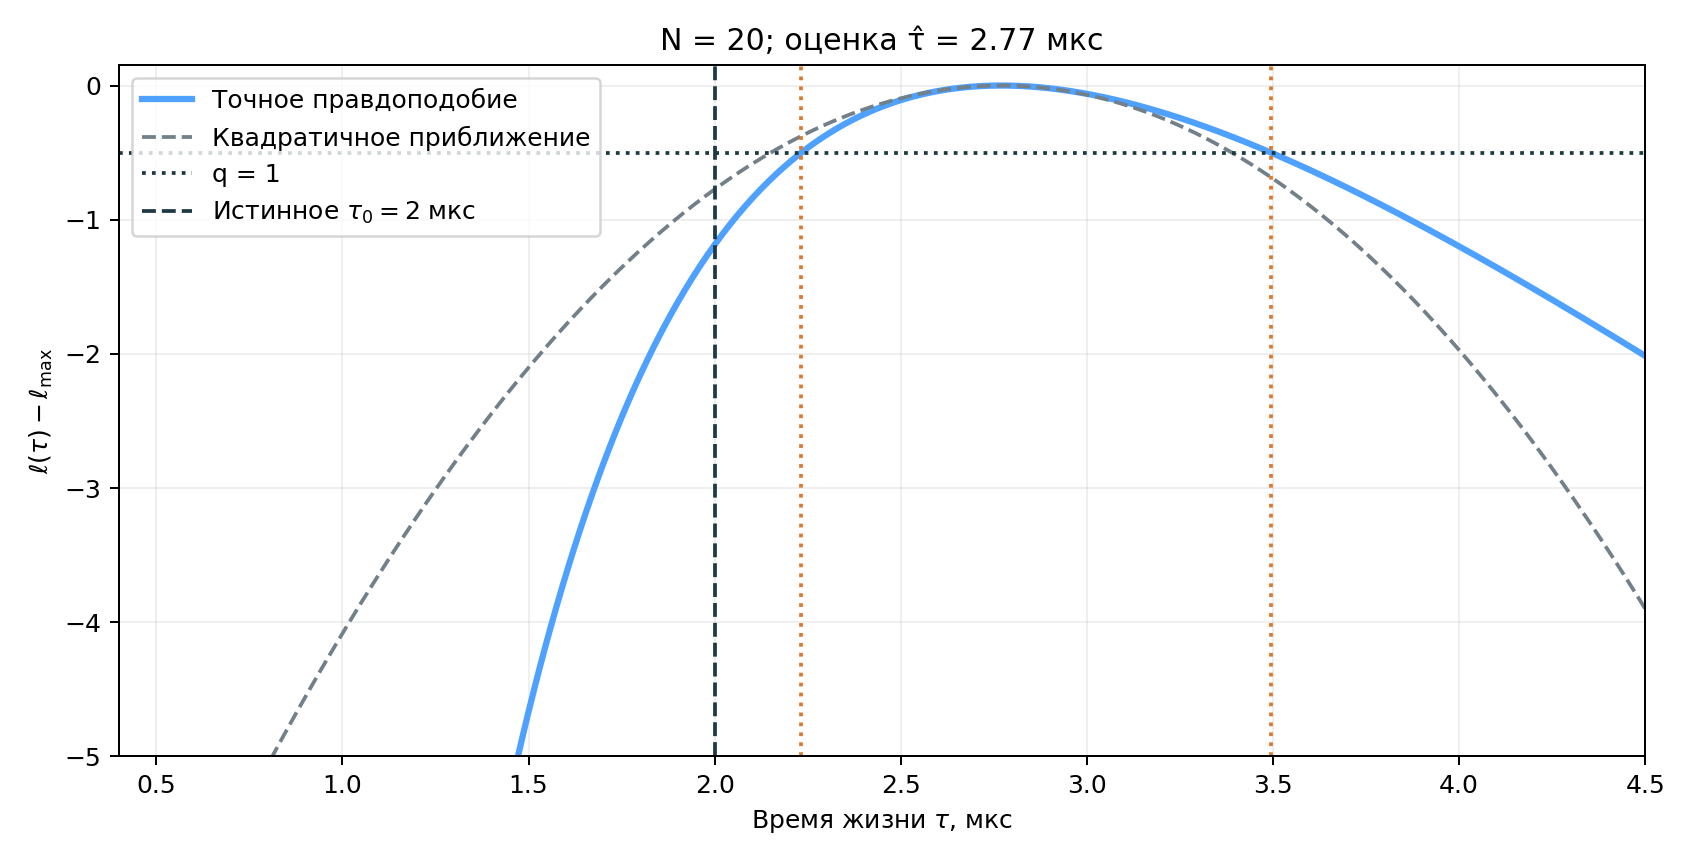
\includegraphics[width=0.74\linewidth,height=\textheight,keepaspectratio,alt={Оценка времени жизни}]{assets/figures/mle_lifetime_n20.png}

\end{center}

\noindent\begin{minipage}[c]{\dimexpr\linewidth-30mm\relax}

\textbf{Интерактив}. \textbf{Оценка времени жизни}

Одна выборка из \(N=20\) распадов при \(\tau_0=2\ \text{мкс}\). Показаны
разность \(\ell(\tau)-\ell_{\max}\), её квадратичное приближение и
границы \(q=1\). Все данные в этом примере сгенерированы.

\end{minipage}\hfill\begin{minipage}[c]{26mm}\centering

\href{https://neutrinohit.github.io/statistical-analysis-course/ru/book/chapters/10_estimator_properties_profile_likelihood.html\#interactive-likelihood-lifetime}{
\includegraphics[width=24mm,height=\textheight,keepaspectratio,alt={QR-код интерактива}]{assets/qr/likelihood-lifetime.png}}

\end{minipage}

\end{semanticpdfbox}

На рисунке \ref{fig-likelihood-lifetime-sample-size} сравниваются две
выборки. При большем \(N\) характерная ширина правдоподобия уменьшается.
Это не обещает, что в каждом следующем опыте оценка будет ближе к
истине: статистические флуктуации сохраняются.

\begin{figure}

\centering{

\pandocbounded{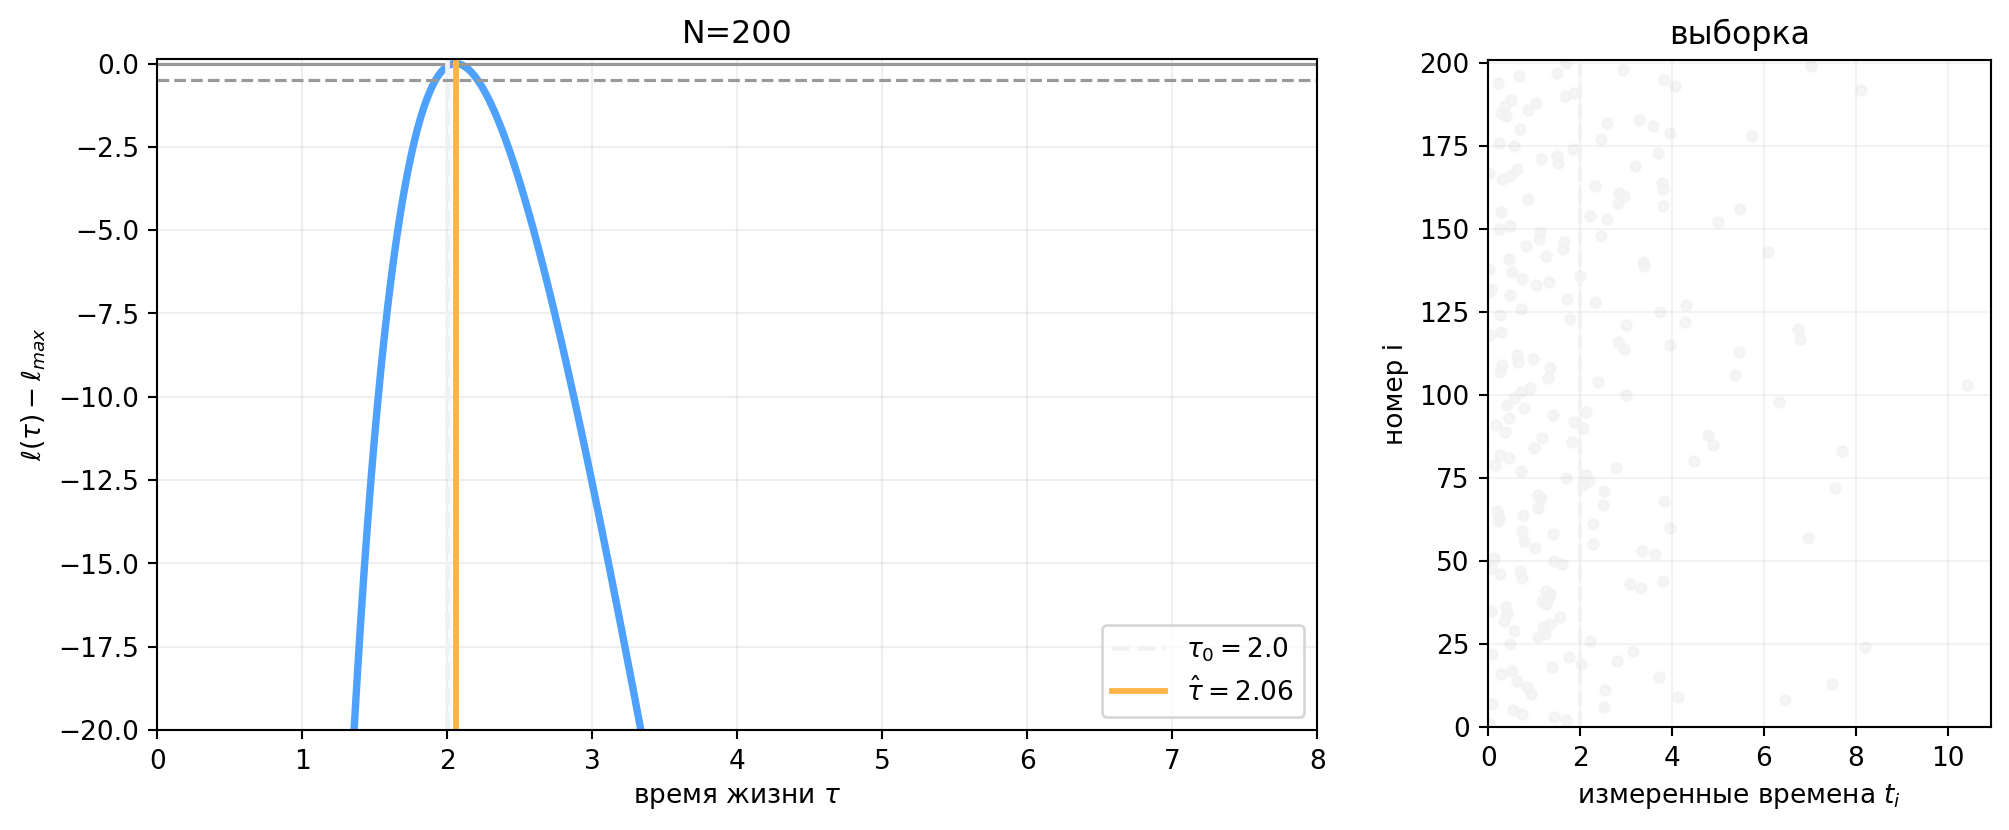
\includegraphics[keepaspectratio]{chapters/../assets/figures/mle_lifetime_n200.png}}

}

\caption{\label{fig-likelihood-lifetime-sample-size}Отношение
правдоподобий для первых 20 и всех 200 времён одной последовательности
распадов при \(\tau_0=2\ \text{мкс}\). Горизонтальная линия задаёт
\(q=1\), вертикальная --- истинное время жизни.}

\end{figure}%

\section{Малые выборки и физические
границы}\label{ux43cux430ux43bux44bux435-ux432ux44bux431ux43eux440ux43aux438-ux438-ux444ux438ux437ux438ux447ux435ux441ux43aux438ux435-ux433ux440ux430ux43dux438ux446ux44b}

Ещё один пример --- пуассоновский счёт. После регистрации \(n\) событий
оценка ожидаемого числа равна \(\widehat\mu=n\). Из пуассоновского
правдоподобия получаем

\begin{equation}\protect\phantomsection\label{eq-ch10-poisson-ratio}{
q(\mu)=2\left[\mu-n+n\ln\frac n\mu\right].
}\end{equation}

При \(n>0\) функция определена для \(\mu>0\). При \(n=0\) используем
предел \(n\ln(n/\mu)=0\), и формула упрощается до

\begin{equation}\protect\phantomsection\label{eq-ch10-zero-count-ratio}{
q(\mu)=2\mu,\qquad\mu\geq0.
}\end{equation}

Максимум \(L\) находится на границе \(\widehat\mu=0\). Никакой параболы
около внутреннего максимума здесь нет. Подстановка \(n=0\) в
приближённую ошибку \(\sqrt n\) дала бы ноль, хотя отсутствие событий не
определяет \(\mu\) с бесконечной точностью.

В таком случае сохраняем полную форму правдоподобия и выбираем процедуру
построения интервала с нужным покрытием. К этим процедурам мы вернёмся в
главах о статистическом выводе.

\section{Несколько
параметров}\label{ux43dux435ux441ux43aux43eux43bux44cux43aux43e-ux43fux430ux440ux430ux43cux435ux442ux440ux43eux432}

Пока у нас был один неизвестный параметр. В эксперименте вместе с ним
обычно приходится определять фон, эффективность, энергетическую шкалу
или разрешение детектора.

Разделим параметры по их роли в данном анализе. \textbf{Параметр
интереса} \(\theta\) --- величина, которую мы хотим измерить. Остальные
обозначим \(\boldsymbol\eta\) и назовём \textbf{мешающими параметрами}
(\emph{nuisance parameters}). Например, при измерении сечения
эффективность мешающая, а в калибровочном опыте из прошлой главы она
сама была параметром интереса.

Сначала найдём совместный максимум:

\begin{equation}\protect\phantomsection\label{eq-ch10-joint-mle}{
(\widehat\theta,\widehat{\boldsymbol\eta})
=\underset{\theta,\boldsymbol\eta}{\operatorname{arg\,max}}
L(\theta,\boldsymbol\eta).
}\end{equation}

Теперь хочется построить зависимость только от \(\theta\). Что делать с
остальными параметрами? Если просто оставить их равными значениям в
совместном максимуме, мы запретим им изменяться при изменении
\(\theta\). При корреляциях это меняет вывод об ошибке.

\subsection{Профильное
правдоподобие}\label{ux43fux440ux43eux444ux438ux43bux44cux43dux43eux435-ux43fux440ux430ux432ux434ux43eux43fux43eux434ux43eux431ux438ux435}

Зафиксируем пробное \(\theta\) и заново найдём максимум по мешающим
параметрам:

\begin{equation}\protect\phantomsection\label{eq-ch10-conditional-nuisance-mle}{
\widehat{\widehat{\boldsymbol\eta}}(\theta)
=\underset{\boldsymbol\eta}{\operatorname{arg\,max}}
L(\theta,\boldsymbol\eta).
}\end{equation}

Двойная шляпка обозначает условный максимум при выбранном \(\theta\).
Повторяя эту операцию для каждого \(\theta\), получим \textbf{профильное
правдоподобие}:

\begin{equation}\protect\phantomsection\label{eq-ch10-profile-likelihood}{
\begin{aligned}
L_{\mathrm p}(\theta)
&=L\!\left(\theta,\widehat{\widehat{\boldsymbol\eta}}(\theta)\right),\\
q_{\mathrm p}(\theta)
&=-2\ln\frac{L_{\mathrm p}(\theta)}
{L(\widehat\theta,\widehat{\boldsymbol\eta})}.
\end{aligned}
}\end{equation}

Это вполне конкретная численная процедура: каждому значению на
горизонтальной оси соответствует своя подгонка мешающих параметров.

\subsection{Двумерный гауссов
пример}\label{interactive-likelihood-profile}

Перенесём начало координат в совместный максимум и измерим отклонения
параметров в единицах их стандартных ошибок. Для гауссовой формы с
корреляцией \(\rho\), \(|\rho|<1\), имеем

\begin{equation}\protect\phantomsection\label{eq-ch10-gaussian-joint-ratio}{
q(\theta,\eta)=
\frac{\theta^2-2\rho\theta\eta+\eta^2}{1-\rho^2}
=\theta^2+\frac{(\eta-\rho\theta)^2}{1-\rho^2}.
}\end{equation}

Вторая запись позволяет найти минимум по \(\eta\). При фиксированном
\(\theta\) он достигается в точке

\begin{equation}\protect\phantomsection\label{eq-ch10-gaussian-profile}{
\widehat{\widehat\eta}(\theta)=\rho\theta,
\qquad
q_{\mathrm p}(\theta)=\theta^2.
}\end{equation}

А сечение при \(\eta=0\) равно

\begin{equation}\protect\phantomsection\label{eq-ch10-gaussian-fixed-slice}{
q(\theta,0)=\frac{\theta^2}{1-\rho^2}.
}\end{equation}

При \(\rho=0.75\) полуширина сечения по уровню \(q=1\) равна
\(\sqrt{1-\rho^2}\simeq0.66\), тогда как профиль даёт единицу. Фиксация
мешающего параметра в его оценённом значении занизила ошибку примерно на
треть. Если же \(\eta\) действительно известен точно из независимых
соображений, фиксация оправданна: это уже другая постановка задачи.

В апплете белая линия на двумерной карте соединяет условные максимумы.
Изменяйте \(\rho\) и следите за разницей между профилем и сечением. При
\(\rho=0\) они совпадут.

\begin{semanticpdfbox}[breakable=false]

\begin{center}

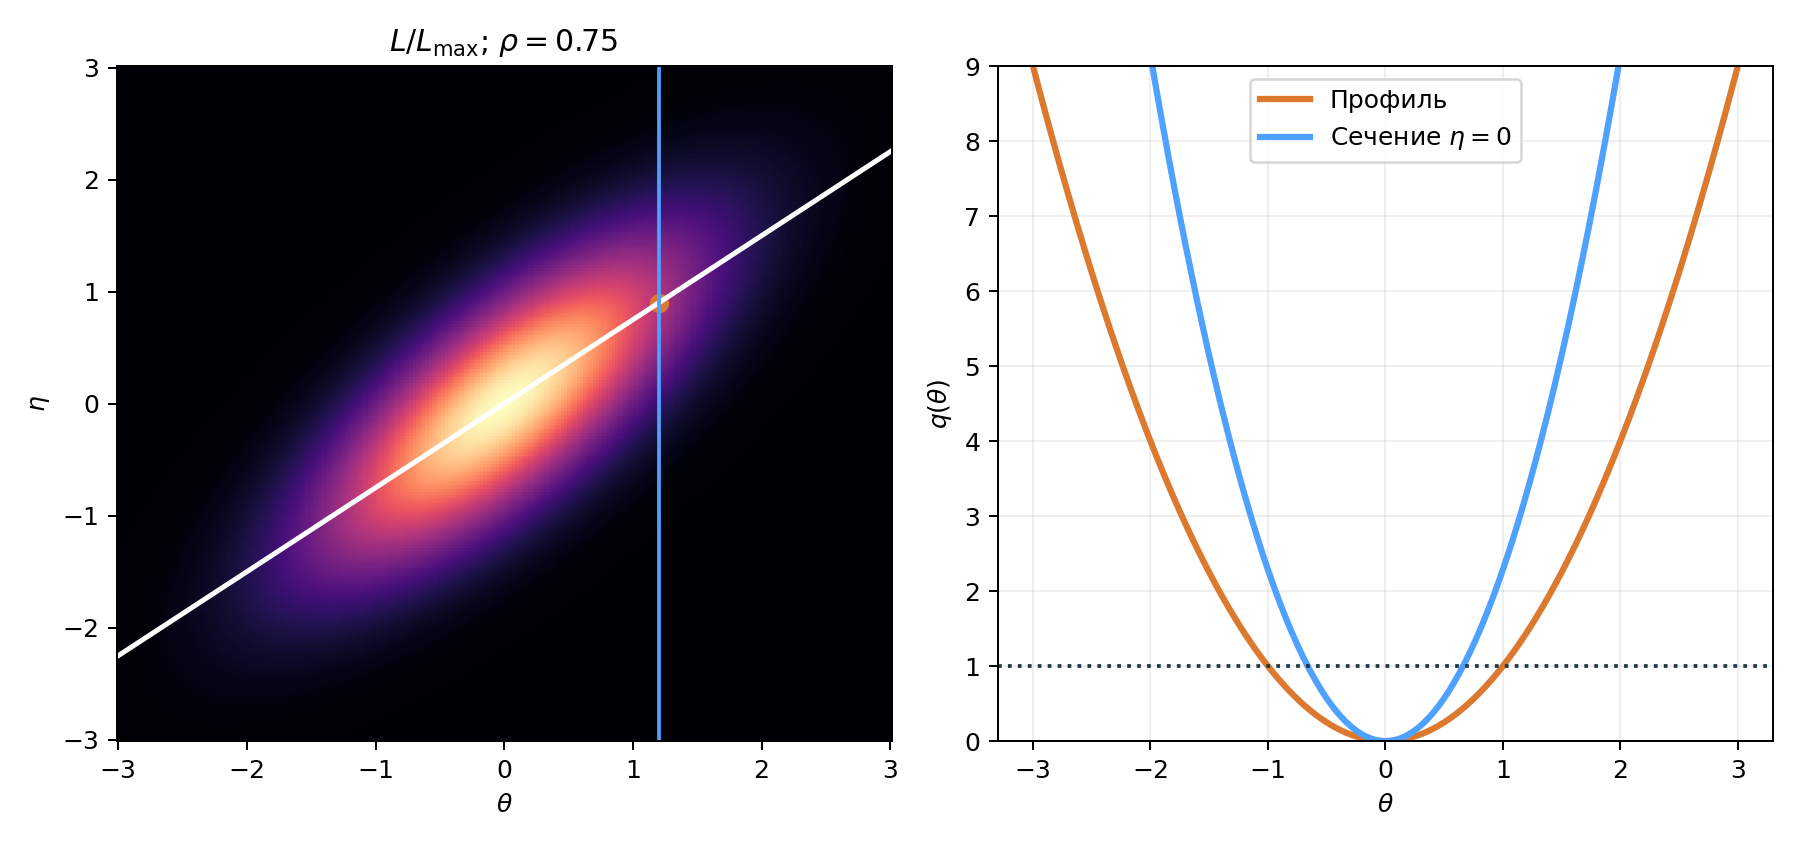
\includegraphics[width=0.74\linewidth,height=\textheight,keepaspectratio,alt={Профиль и фиксированное сечение}]{assets/figures/mle_profile_likelihood_rho075.png}

\end{center}

\noindent\begin{minipage}[c]{\dimexpr\linewidth-30mm\relax}

\textbf{Интерактив}. \textbf{Профиль и фиксированное сечение}

Двумерное относительное правдоподобие при \(\rho=0.75\) и две одномерные
кривые: профиль \(q_{\mathrm p}(\theta)\) и сечение \(q(\theta,0)\).
Белая линия показывает \(\widehat{\widehat\eta}(\theta)=\rho\theta\).

\end{minipage}\hfill\begin{minipage}[c]{26mm}\centering

\href{https://neutrinohit.github.io/statistical-analysis-course/ru/book/chapters/10_estimator_properties_profile_likelihood.html\#interactive-likelihood-profile}{
\includegraphics[width=24mm,height=\textheight,keepaspectratio,alt={QR-код интерактива}]{assets/qr/likelihood-profile.png}}

\end{minipage}

\end{semanticpdfbox}

\section{Пример: реакторные
нейтрино}\label{ux43fux440ux438ux43cux435ux440-ux440ux435ux430ux43aux442ux43eux440ux43dux44bux435-ux43dux435ux439ux442ux440ux438ux43dux43e}

Перейдём от гауссовой поверхности к физической модели. Детектор
находится на расстоянии \(L=1600\ \text{м}\) от реактора. По
энергетическому спектру зарегистрированных антинейтрино требуется
оценить два осцилляционных параметра: амплитуду \(A=\sin^2(2\theta)\) и
разность квадратов масс \(\Delta m^2\).

Возьмём двухфлейворную вакуумную вероятность выживания:

\begin{equation}\protect\phantomsection\label{eq-ch10-reactor-survival}{
P_{ee}(E;A,\Delta m^2)
=1-A\sin^2\!\left(1.267\,\Delta m^2\frac LE\right).
}\end{equation}

В этой записи \(\Delta m^2\) выражается в \(\text{эВ}^2\), \(L\) --- в
метрах, \(E\) --- в МэВ. Амплитуда задаёт глубину осцилляционного
провала, а \(\Delta m^2\) меняет его положение по энергии.

Это учебная модель. Будем считать расстояние, нормировку и спектр
источника известными точно; фон и энергетическое разрешение пока
отсутствуют. Измеряемая энергия здесь совпадает с энергией антинейтрино.
В реальном детекторе наблюдается энергия продуктов взаимодействия, и для
связи с \(E\) нужна модель отклика.

\subsection{Ожидаемое число
событий}\label{ux43eux436ux438ux434ux430ux435ux43cux43eux435-ux447ux438ux441ux43bux43e-ux441ux43eux431ux44bux442ux438ux439}

Разобьём энергетический диапазон на бины. Если \(\phi(E)\) описывает
спектр источника, а \(\sigma(E)\) --- сечение регистрации, то среднее
число событий в бине равно

\begin{equation}\protect\phantomsection\label{eq-ch10-reactor-bin-integral}{
\mu_i(A,\Delta m^2)
=C\int_{E_i^-}^{E_i^+}
\phi(E)\sigma(E)P_{ee}(E;A,\Delta m^2)\,dE.
}\end{equation}

В апплете интеграл приближён значением подынтегральной функции в центре
бина, умноженным на его ширину:

\begin{equation}\protect\phantomsection\label{eq-ch10-reactor-midpoint-model}{
\mu_i\simeq C\,\phi(E_i)\sigma(E_i)
P_{ee}(E_i;A,\Delta m^2)\Delta E_i.
}\end{equation}

Одно и то же приближение используется при генерации и подгонке. Для
анализа реальных данных точность интегрирования по бину проверяется
отдельно.

Числа событий в непересекающихся бинах моделируем независимыми
пуассоновскими величинами \(n_i\sim\operatorname{Pois}(\mu_i)\). Тогда с
точностью до константы

\begin{equation}\protect\phantomsection\label{eq-reactor-log-likelihood}{
\ell(A,\Delta m^2)
=\sum_i\left[n_i\ln\mu_i(A,\Delta m^2)
-\mu_i(A,\Delta m^2)\right].
}\end{equation}

Эту функцию и предстоит максимизировать.

\subsection{Спектр источника и
сечение}\label{ux441ux43fux435ux43aux442ux440-ux438ux441ux442ux43eux447ux43dux438ux43aux430-ux438-ux441ux435ux447ux435ux43dux438ux435}

Используем параметризацию спектров Хубера и Мюллера {[}3, 4{]}:

\begin{equation}\protect\phantomsection\label{eq-ch10-reactor-flux}{
\phi(E)=\sum_k f_k
\exp\!\left[\sum_{p=0}^{5}a_{kp}(E/\text{МэВ})^p\right].
}\end{equation}

Индекс \(k\) нумерует четыре делящихся изотопа, \(f_k\) --- их доли
делений. Общую размерную нормировку спектра включаем в \(C\).
Коэффициенты приведены в таблице
\ref{tbl-reactor-spectrum-coefficients}. Доли выбраны для примера и во
время расчёта не меняются. Продолжение параметризации ниже
\(2\ \text{МэВ}\) также используется только как учебное приближение.

\begin{longtable}[]{@{}
  >{\raggedright\arraybackslash}p{(\linewidth - 8\tabcolsep) * \real{0.1163}}
  >{\raggedleft\arraybackslash}p{(\linewidth - 8\tabcolsep) * \real{0.2093}}
  >{\raggedleft\arraybackslash}p{(\linewidth - 8\tabcolsep) * \real{0.2093}}
  >{\raggedleft\arraybackslash}p{(\linewidth - 8\tabcolsep) * \real{0.2326}}
  >{\raggedleft\arraybackslash}p{(\linewidth - 8\tabcolsep) * \real{0.2326}}@{}}
\caption{Доли делений и коэффициенты спектров в учебной
модели}\label{tbl-reactor-spectrum-coefficients}\tabularnewline
\toprule\noalign{}
\begin{minipage}[b]{\linewidth}\raggedright
Величина
\end{minipage} & \begin{minipage}[b]{\linewidth}\raggedleft
\(^{235}\mathrm U\)
\end{minipage} & \begin{minipage}[b]{\linewidth}\raggedleft
\(^{238}\mathrm U\)
\end{minipage} & \begin{minipage}[b]{\linewidth}\raggedleft
\(^{239}\mathrm{Pu}\)
\end{minipage} & \begin{minipage}[b]{\linewidth}\raggedleft
\(^{241}\mathrm{Pu}\)
\end{minipage} \\
\midrule\noalign{}
\endfirsthead
\toprule\noalign{}
\begin{minipage}[b]{\linewidth}\raggedright
Величина
\end{minipage} & \begin{minipage}[b]{\linewidth}\raggedleft
\(^{235}\mathrm U\)
\end{minipage} & \begin{minipage}[b]{\linewidth}\raggedleft
\(^{238}\mathrm U\)
\end{minipage} & \begin{minipage}[b]{\linewidth}\raggedleft
\(^{239}\mathrm{Pu}\)
\end{minipage} & \begin{minipage}[b]{\linewidth}\raggedleft
\(^{241}\mathrm{Pu}\)
\end{minipage} \\
\midrule\noalign{}
\endhead
\bottomrule\noalign{}
\endlastfoot
\(f_k\) & 0.58 & 0.07 & 0.30 & 0.05 \\
\(a_0\) & 4.367 & 0.4833 & 4.757 & 2.990 \\
\(a_1\) & -4.577 & 0.1927 & -5.392 & -2.882 \\
\(a_2\) & 2.100 & -0.1283 & 2.563 & 1.278 \\
\(a_3\) & -0.5294 & -0.006762 & -0.6596 & -0.3343 \\
\(a_4\) & 0.06186 & 0.002233 & 0.07820 & 0.03905 \\
\(a_5\) & -0.002777 & -0.0001536 & -0.003536 & -0.001754 \\
\end{longtable}

Регистрация происходит через обратный бета-распад
\(\overline\nu_e+p\to e^++n\). В приближении без отдачи нуклонов
энергетическая зависимость сечения имеет вид

\begin{equation}\protect\phantomsection\label{eq-ch10-reactor-cross-section}{
\sigma(E)\propto E_ep_e,
\qquad
E_e=E-1.293\ \text{МэВ},
\qquad
p_e=\sqrt{E_e^2-m_e^2},
}\end{equation}

где \(m_e=0.511\ \text{МэВ}\), \(c=1\). Ниже порога в модели полагаем
сечение равным нулю. Поправки на отдачу здесь не учитываются. Диапазон
расчёта составляет \(1.8\)--\(8\ \text{МэВ}\), а \(C\) выбирается так,
чтобы без осцилляций ожидаемое полное число событий равнялось заданному
\(N_0\).

\subsection{Генерация и
подгонка}\label{interactive-likelihood-reactor-oscillation}

Сначала зададим истинные \(A_0\) и \(\Delta m_0^2\), вычислим средние
числа событий и сгенерируем пуассоновские \(n_i\). Полученные
псевдоданные зафиксируем. Теперь переберём пробные пары
\((A,\Delta m^2)\) и для каждой посчитаем логарифм правдоподобия
\ref{eq-reactor-log-likelihood}.

В апплете используется сетка из \(61\times61\) точки. Максимум и профили
находятся именно на этой сетке:

\begin{equation}\protect\phantomsection\label{eq-ch10-reactor-profiles}{
\begin{aligned}
q(A,\Delta m^2)&=-2[\ell(A,\Delta m^2)-\ell_{\max}],\\
q_{\mathrm p}(A)&=\min_{\Delta m^2}q(A,\Delta m^2),\\
q_{\mathrm p}(\Delta m^2)&=\min_A q(A,\Delta m^2).
\end{aligned}
}\end{equation}

Здесь оба параметра представляют физический интерес. Но при построении
одномерного профиля одного из них второй играет роль мешающего.

\begin{semanticpdfbox}[breakable=false]

\begin{center}

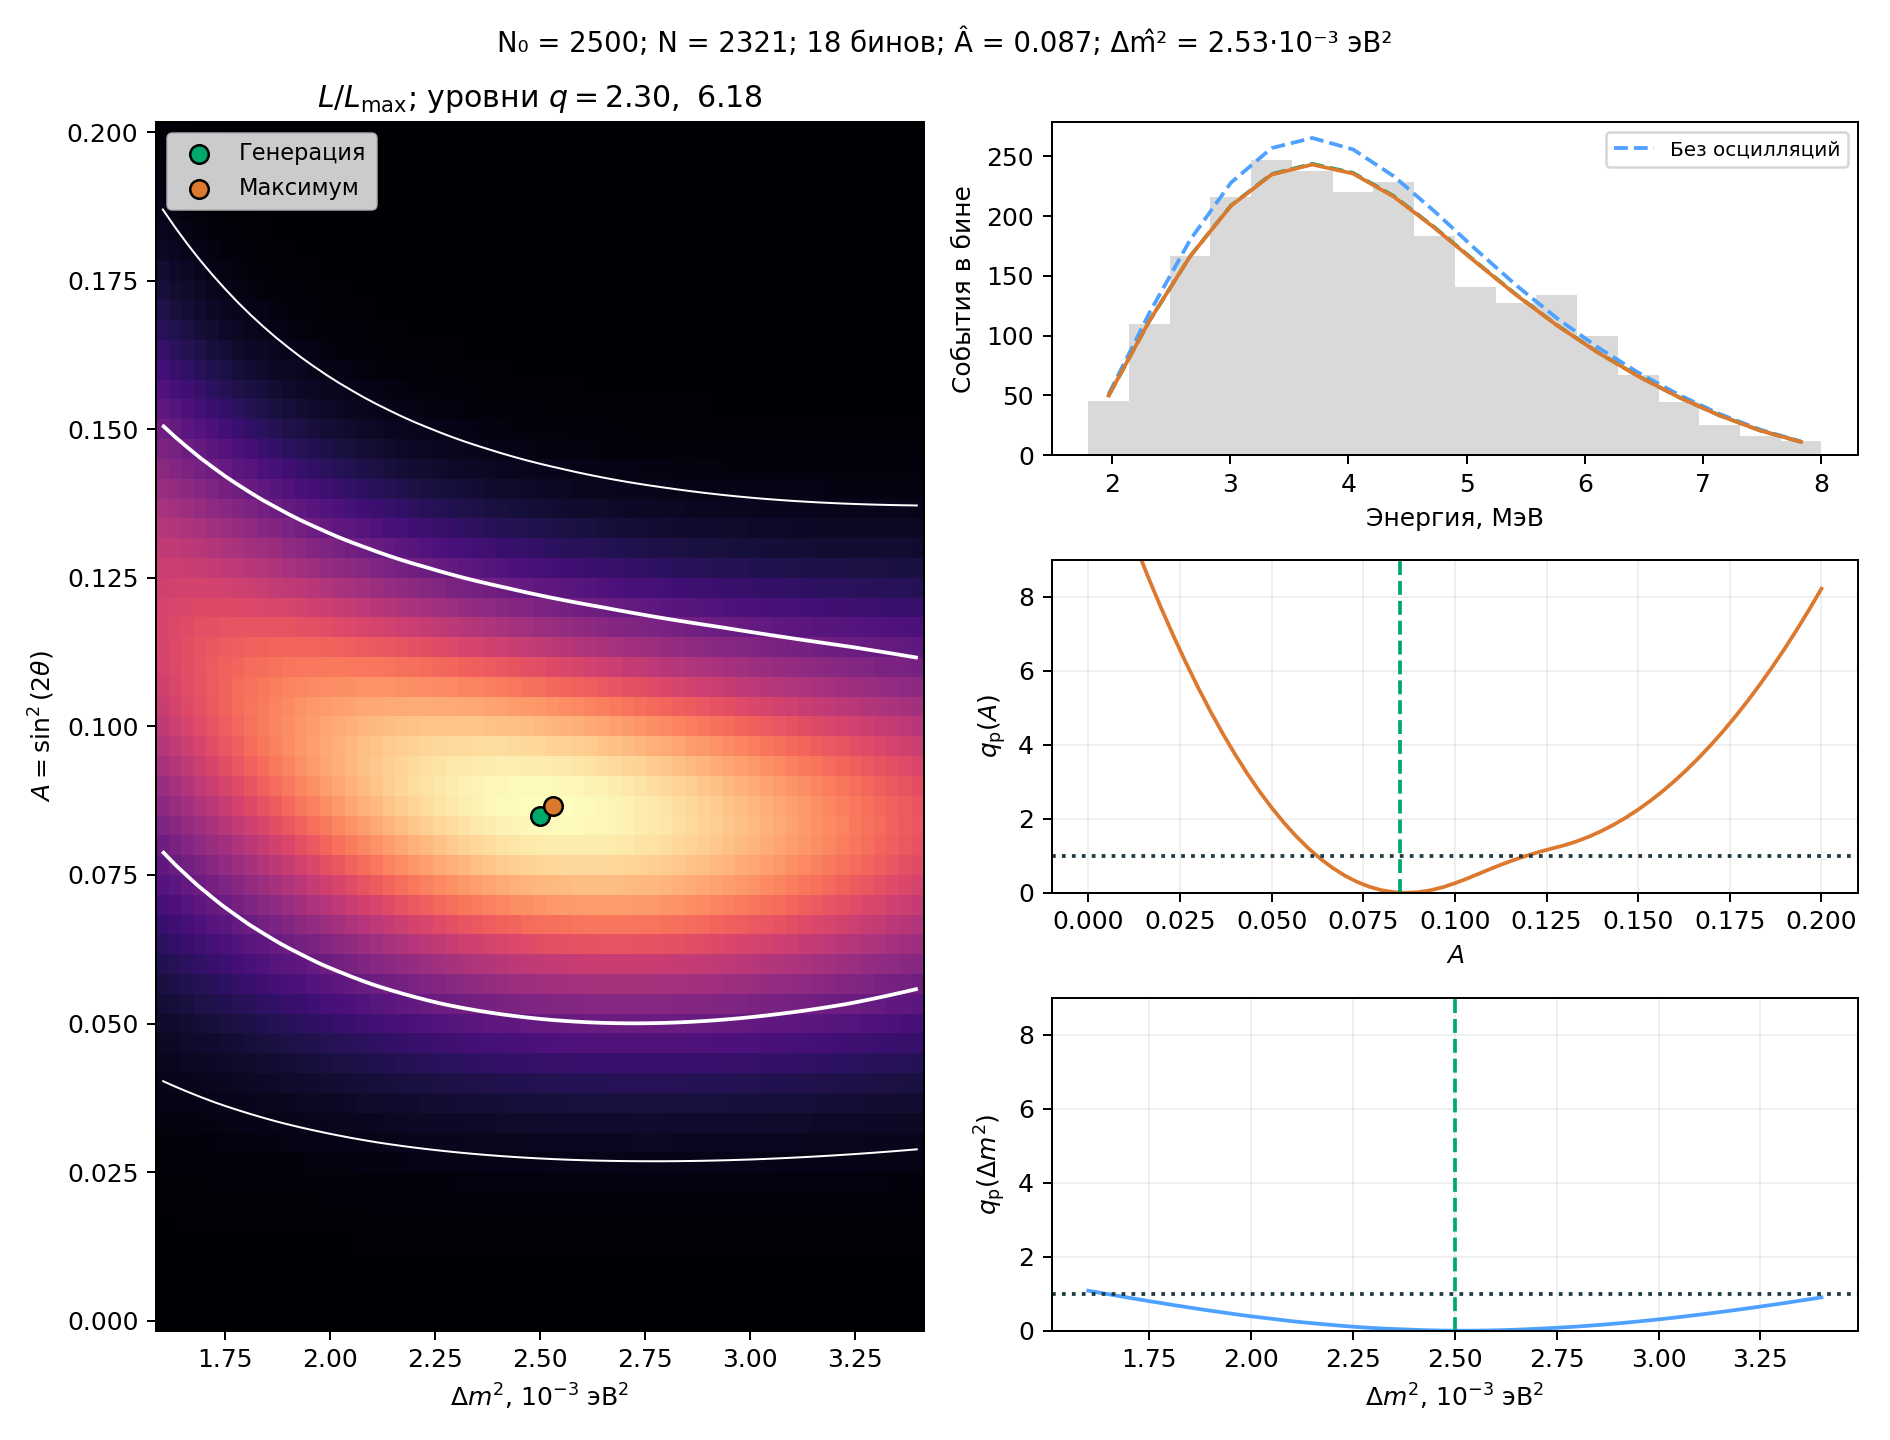
\includegraphics[width=0.74\linewidth,height=\textheight,keepaspectratio,alt={Подгонка реакторного спектра}]{assets/figures/mle_reactor_oscillation_default.png}

\end{center}

\noindent\begin{minipage}[c]{\dimexpr\linewidth-30mm\relax}

\textbf{Интерактив}. \textbf{Подгонка реакторного спектра}

Псевдоэксперимент при \(N_0=2500\), \(A_0=0.085\),
\(\Delta m_0^2=2.5\cdot10^{-3}\ \text{эВ}^2\) и 18 энергетических бинах.
Зелёным обозначены параметры генерации, оранжевым --- максимум на сетке.
Показаны двумерное правдоподобие, спектр событий и два одномерных
профиля.

\end{minipage}\hfill\begin{minipage}[c]{26mm}\centering

\href{https://neutrinohit.github.io/statistical-analysis-course/ru/book/chapters/10_estimator_properties_profile_likelihood.html\#interactive-likelihood-reactor-oscillation}{
\includegraphics[width=24mm,height=\textheight,keepaspectratio,alt={QR-код интерактива}]{assets/qr/likelihood-reactor-oscillation.png}}

\end{minipage}

\end{semanticpdfbox}

Начните с энергетического спектра. Насколько похожи кривые для истинных
параметров и для найденного максимума? Затем посмотрите на двумерную
карту. Разные пары параметров могут давать близкие спектры, поэтому
область большого правдоподобия вытягивается. По одномерным профилям
видно, насколько каждый параметр можно изменить, подстраивая второй.

На карте отмечены уровни \(q=2.30\) и \(q=6.18\). В регулярном гауссовом
пределе они соответствуют совместным областям с покрытием примерно
\(68.3\%\) и \(95.4\%\) для двух параметров. Уровень \(q_{\mathrm p}=1\)
относится к одному профилируемому параметру. Разницу между одномерными и
двумерными порогами мы уже видели при построении гауссовых эллипсов.

В этой модели есть место, где ссылка на гауссов предел особенно опасна.
При \(A=0\) вероятность \(P_{ee}=1\) вообще не зависит от
\(\Delta m^2\): данные не могут определить частоту осцилляций, если их
амплитуда равна нулю. Нарушается идентифицируемость параметра. Поэтому
показанные уровни служат ориентирами; точность покрытия около \(A=0\)
надо проверять псевдоэкспериментами.

Увеличьте \(N_0\) и повторите генерацию. Статистический разброс
уменьшается, детали спектра становятся лучше различимы. Если максимум
оказался на краю сетки, проверьте сам диапазон поиска. Границы
\(A\leq0.20\) и \(1.6\leq\Delta m^2/(10^{-3}\ \text{эВ}^2)\leq3.4\)
выбраны для апплета. Они не являются полными физическими границами
осцилляционных параметров.

\section{Правдоподобие в реальном
анализе}\label{ux43fux440ux430ux432ux434ux43eux43fux43eux434ux43eux431ux438ux435-ux432-ux440ux435ux430ux43bux44cux43dux43eux43c-ux430ux43dux430ux43bux438ux437ux435}

\subsection{Вспомогательное
измерение}\label{ux432ux441ux43fux43eux43cux43eux433ux430ux442ux435ux43bux44cux43dux43eux435-ux438ux437ux43cux435ux440ux435ux43dux438ux435}

Пусть неизвестный фон или калибровку \(\eta\) дополнительно измерили в
независимом опыте. Результат \(a\) описывается моделью
\(a\sim\mathcal N(\eta,\sigma_a^2)\) с известной \(\sigma_a\). Тогда
полное правдоподобие равно

\begin{equation}\protect\phantomsection\label{eq-ch10-auxiliary-likelihood}{
L_{\mathrm{полн}}(\theta,\eta)
=L_{\mathrm{осн}}(\theta,\eta)
\exp\!\left[-\frac{(a-\eta)^2}{2\sigma_a^2}\right]
\times\mathrm{const}.
}\end{equation}

Гауссов множитель описывает распределение результата вспомогательного
измерения при заданном \(\eta\). Его происхождение то же, что у основной
функции правдоподобия. При профилировании мы максимизируем произведение
обоих множителей. В каждом условном максимуме учитываются и основные, и
калибровочные данные.

\subsection{Расширенное
правдоподобие}\label{ux440ux430ux441ux448ux438ux440ux435ux43dux43dux43eux435-ux43fux440ux430ux432ux434ux43eux43fux43eux434ux43eux431ux438ux435}

Во многих экспериментах информация заключена одновременно в форме
спектра и в полном числе событий. Пусть \(f(x\mid\boldsymbol\theta)\)
--- нормированная плотность признака одного события, а
\(\nu(\boldsymbol\theta)\) --- ожидаемое число зарегистрированных
событий. При пуассоновском счёте и независимых событиях
\textbf{расширенное правдоподобие} равно

\begin{equation}\protect\phantomsection\label{eq-ch10-extended-likelihood}{
L_{\mathrm{расш}}(\boldsymbol\theta)
=\frac{e^{-\nu}\nu^N}{N!}
\prod_{i=1}^{N}f(x_i\mid\boldsymbol\theta).
}\end{equation}

Пуассоновский множитель использует число событий; произведение
плотностей описывает их распределение по \(x\).

Например, ожидается \(s\) сигнальных и \(b\) фоновых событий с
нормированными плотностями \(f_s\) и \(f_b\). Тогда \(\nu=s+b\) и

\[
f(x)=\frac{s f_s(x)+b f_b(x)}{s+b}.
\]

После подстановки множители \((s+b)^N\) сокращаются:

\begin{equation}\protect\phantomsection\label{eq-ch10-extended-signal-background}{
L_{\mathrm{расш}}(s,b)
=\frac{e^{-(s+b)}}{N!}
\prod_{i=1}^{N}[s f_s(x_i)+b f_b(x_i)].
}\end{equation}

Можно добавить вспомогательное измерение фона и профилировать по \(b\).
Так получается модель, в которой число событий, форма спектра и
измерение фона участвуют в одной подгонке.

\subsection{Правдоподобие для
гистограммы}\label{ux43fux440ux430ux432ux434ux43eux43fux43eux434ux43eux431ux438ux435-ux434ux43bux44f-ux433ux438ux441ux442ux43eux433ux440ux430ux43cux43cux44b}

Если сохранить только числа событий в бинах, расширенное правдоподобие
переходит в произведение пуассоновских вероятностей:

\begin{equation}\protect\phantomsection\label{eq-ch10-binned-poisson-likelihood}{
L(\boldsymbol\theta)
=\prod_j\frac{e^{-\mu_j(\boldsymbol\theta)}
\mu_j(\boldsymbol\theta)^{n_j}}{n_j!}.
}\end{equation}

Именно такую запись мы использовали для реакторного спектра.
Независимость счётчиков соответствует пуассоновскому полному числу
событий. Если полное число \(N\) фиксировано условием опыта,
распределение чисел по бинам будет мультиномиальным: сумма \(n_j=N\)
связывает их между собой.

Гистограмма сокращает вычисления. Вместо миллионов событий можно
работать с несколькими десятками или сотнями бинов. Цена слишком грубого
разбиения --- потеря информации о положении событий внутри бина.
Например, узкий пик может целиком оказаться в одном широком бине:
определить по нему положение пика будет трудно.

\subsection{Замена
параметров}\label{ux437ux430ux43cux435ux43dux430-ux43fux430ux440ux430ux43cux435ux442ux440ux43eux432}

Пусть нам удобнее подгонять \(\phi=g(\theta)\), где \(g\) взаимно
однозначна. Правдоподобие в новой переменной равно \(L(g^{-1}(\phi))\),
поэтому

\begin{equation}\protect\phantomsection\label{eq-ch10-mle-invariance}{
\widehat\phi_{\mathrm{ММП}}=g(\widehat\theta_{\mathrm{ММП}}).
}\end{equation}

Это свойство называется \textbf{инвариантностью ММП}. Например, для
скорости распада \(\lambda=1/\tau\) получаем
\(\widehat\lambda=1/\overline t\). Якобиан здесь не появляется: мы
меняем аргумент функции правдоподобия. Преобразование плотности
случайной величины --- другая операция.

Несмещённость при нелинейной замене может потеряться, поскольку
\(\mathbb E[g(\widehat\theta)]\) в общем случае не равно
\(g(\mathbb E[\widehat\theta])\). Границы интервала также надо
преобразовывать самостоятельно. Для \(\lambda=1/\tau\) интервал
\([\tau_-,\tau_+]\) переходит в \([1/\tau_+,1/\tau_-]\).

\section{Проверка численной
подгонки}\label{ux43fux440ux43eux432ux435ux440ux43aux430-ux447ux438ux441ux43bux435ux43dux43dux43eux439-ux43fux43eux434ux433ux43eux43dux43aux438}

В простых примерах максимум мы нашли аналитически. В большой модели его
ищет программа, и сообщение о сходимости само по себе не проверяет ни
статистическую модель, ни глобальность максимума.

Начните с повторных запусков из разных начальных точек. Сравните
значения логарифма правдоподобия и проверьте градиент во внутреннем
максимуме. Затем постройте профили и двумерные сечения для коррелирующих
параметров. Несколько типичных ситуаций собраны в таблице
\ref{tbl-likelihood-fit-problems}.

\begin{longtable}[]{@{}
  >{\raggedright\arraybackslash}p{(\linewidth - 2\tabcolsep) * \real{0.5161}}
  >{\raggedright\arraybackslash}p{(\linewidth - 2\tabcolsep) * \real{0.4839}}@{}}
\caption{Проверки численной
подгонки}\label{tbl-likelihood-fit-problems}\tabularnewline
\toprule\noalign{}
\begin{minipage}[b]{\linewidth}\raggedright
Что получилось
\end{minipage} & \begin{minipage}[b]{\linewidth}\raggedright
Что проверить
\end{minipage} \\
\midrule\noalign{}
\endfirsthead
\toprule\noalign{}
\begin{minipage}[b]{\linewidth}\raggedright
Что получилось
\end{minipage} & \begin{minipage}[b]{\linewidth}\raggedright
Что проверить
\end{minipage} \\
\midrule\noalign{}
\endhead
\bottomrule\noalign{}
\endlastfoot
Разные результаты из разных начальных точек & Локальные максимумы и
точность оптимизации \\
Максимум на краю диапазона поиска & Физическая ли это граница или только
настройка программы \\
Почти плоский профиль & Чувствительность данных к параметру и возможное
вырождение \\
Узкое сечение и широкий профиль & Корреляцию с мешающими параметрами \\
\texttt{NaN} или бесконечность & Допустимость параметров, вычисление
логарифмов и нормировок \\
\end{longtable}

После этого повторите весь анализ на псевдоэкспериментах. Истинные
параметры в них известны: можно измерить смещение оценки, её дисперсию и
частоту попадания на границу. Сравните разброс оценок с ошибкой по
кривизне. Если строите интервалы, посчитайте долю интервалов, накрывших
истинное значение. Так проверяется покрытие всей принятой процедуры.

Псевдоэксперименты из той же модели проверяют работу метода внутри этой
модели. Чтобы исследовать неверное описание фона или отклика детектора,
нужно отдельно менять модель генерации. Подгонка к реальным данным
требует также проверки согласия; ей будут посвящены следующие главы.

\begin{bookchaptersummary}[Итоги главы]

\begin{itemize}
\tightlist
\item
  Средний квадрат ошибки складывается из дисперсии и квадрата смещения.
  Несмещённость, состоятельность и малый разброс --- разные свойства
  оценки.
\item
  Информация Фишера задаёт границу дисперсии несмещённых оценок при
  условиях регулярности. Обратная кривизна конкретного правдоподобия
  даёт локальную оценку ошибки; при малой выборке или на границе её надо
  проверять.
\item
  При профилировании мешающие параметры заново подгоняются для каждого
  значения параметра интереса. Фиксация в совместном максимуме при
  корреляциях даёт другую, более узкую кривую.
\item
  Псевдоэксперименты позволяют проверить смещение, разброс и покрытие
  интервалов. Асимптотические пороги отношения правдоподобий требуют
  отдельной проверки там, где нарушаются их условия применимости.
\end{itemize}

\end{bookchaptersummary}

\section{Задачи}\label{ux437ux430ux434ux430ux447ux438-9}

\begin{semanticpdfbox}[colback=BookCoralSoft,borderline west={1.2mm}{0pt}{BookCoral},breakable=false]

\noindent{\sffamily\bfseries\fontsize{11.2}{13.5}\selectfont Задача 1. Информация Фишера для гауссова среднего}\par\nopagebreak[4]\vspace{1.2mm}

Пусть \[
X_i\sim\mathrm N(\mu,\sigma^2),
\] где измерения независимы, а \(\sigma\) известна.

\begin{enumerate}
\def\labelenumi{\arabic{enumi}.}
\tightlist
\item
  Вычислите информацию Фишера для одного наблюдения и всей выборки.
\item
  Получите границу Крамера--Рао для дисперсии несмещённой оценки
  \(\mu\).
\item
  Сравните границу с дисперсией выборочного среднего.
\end{enumerate}

\end{semanticpdfbox}

\begin{semanticpdfbox}[colback=BookCoralSoft,borderline west={1.2mm}{0pt}{BookCoral},breakable=false]

\noindent{\sffamily\bfseries\fontsize{11.2}{13.5}\selectfont Задача 2. Смещённая оценка дисперсии}\par\nopagebreak[4]\vspace{1.2mm}

Для независимой гауссовой выборки размера \(N\geq2\) с неизвестными
\(\mu\) и \(\sigma^2\):

\begin{enumerate}
\def\labelenumi{\arabic{enumi}.}
\tightlist
\item
  Найдите оценки максимального правдоподобия обоих параметров.
\item
  Покажите, что \[
  \mathbb E[\widehat{\sigma^2}_{\mathrm{ММП}}]
  =
  \frac{N-1}{N}\sigma^2.
  \]
\item
  Постройте несмещённую оценку дисперсии.
\item
  Сравните средние квадраты ошибок двух оценок аналитически или методом
  Монте-Карло.
\item
  Обсудите, почему оценка максимального правдоподобия не обязана быть
  несмещённой при конечном \(N\).
\end{enumerate}

\end{semanticpdfbox}

\begin{semanticpdfbox}[colback=BookCoralSoft,borderline west={1.2mm}{0pt}{BookCoral},breakable=false]

\noindent{\sffamily\bfseries\fontsize{11.2}{13.5}\selectfont Задача 3. Профилирование мешающего параметра}\par\nopagebreak[4]\vspace{1.2mm}

Рассмотрите квадратичный логарифм функции правдоподобия \[
-2\ell(\theta,\eta)
=
\frac{\theta^2-2\rho\theta\eta+\eta^2}{1-\rho^2}
+\mathrm{const},
\qquad |\rho|<1.
\]

\begin{enumerate}
\def\labelenumi{\arabic{enumi}.}
\tightlist
\item
  Найдите совместный максимум.
\item
  Для фиксированного \(\theta\) найдите \[
  \widehat{\widehat\eta}(\theta).
  \]
\item
  Постройте профильную функцию \(q_{\mathrm{p}}(\theta)\).
\item
  Сравните её с сечением \(q(\theta,\eta=0)\).
\item
  Объясните, почему фиксация \(\eta\) в его оценке занижает
  неопределённость при \(\rho\ne0\). Как изменится постановка задачи,
  если \(\eta\) известен точно?
\end{enumerate}

\end{semanticpdfbox}

\begin{semanticpdfbox}[colback=BookCoralSoft,borderline west={1.2mm}{0pt}{BookCoral},breakable=false]

\noindent{\sffamily\bfseries\fontsize{11.2}{13.5}\selectfont Задача 4. Расширенная функция правдоподобия для сигнала и фона}\par\nopagebreak[4]\vspace{1.2mm}

Наблюдаются события с признаком \(x\). Ожидаемые числа сигнала и фона
равны \(s\) и \(b\), а нормированные плотности --- \(f_s(x)\) и
\(f_b(x)\).

\begin{enumerate}
\def\labelenumi{\arabic{enumi}.}
\tightlist
\item
  Запишите расширенную функцию правдоподобия для выборки
  \(x_1,\ldots,x_N\).
\item
  Покажите, как в ней используются число событий и форма распределения.
\item
  Запишите функцию правдоподобия для бинированных данных.
\item
  Обсудите, какая информация теряется при грубом биннировании.
\item
  Независимое вспомогательное измерение фона дало \(a\) и описывается
  моделью \(a\sim\mathcal N(b,\sigma_a^2)\) с известной \(\sigma_a\).
  Добавьте его в полное правдоподобие и укажите, по какому параметру
  надо профилировать при оценивании \(s\).
\end{enumerate}

\end{semanticpdfbox}

\begin{semanticpdfbox}[colback=BookCoralSoft,borderline west={1.2mm}{0pt}{BookCoral},breakable=false]

\noindent{\sffamily\bfseries\fontsize{11.2}{13.5}\selectfont Задача 5. Проверка подгонки на псевдоэкспериментах}\par\nopagebreak[4]\vspace{1.2mm}

Выберите одну из моделей предыдущих задач.

\begin{enumerate}
\def\labelenumi{\arabic{enumi}.}
\tightlist
\item
  Сгенерируйте не менее \(5000\) псевдоэкспериментов при известном
  истинном параметре.
\item
  В каждом псевдоэксперименте найдите оценку максимального
  правдоподобия.
\item
  Оцените смещение, дисперсию и средний квадрат ошибки.
\item
  Исследуйте зависимость результатов от размера выборки.
\item
  Если выбранная модель имеет физическую границу параметра, проверьте,
  как часто оценка попадает на неё.
\item
  Сравните фактический разброс оценки максимального правдоподобия с
  ошибкой, предсказанной кривизной логарифма функции правдоподобия.
\end{enumerate}

\end{semanticpdfbox}

\section*{Литература}\label{ux43bux438ux442ux435ux440ux430ux442ux443ux440ux430-9}
\addcontentsline{toc}{section}{Литература}

\markright{Литература}

\protect\phantomsection\label{refs}
\begin{CSLReferences}{0}{0}
\bibitem[\citeproctext]{ref-cowan1998}
{[}1{]} Cowan, G. \emph{Statistical Data Analysis}. Oxford University
Press. 1998.

\bibitem[\citeproctext]{ref-wilks1938}
{[}2{]} Wilks, S. S. The Large-Sample Distribution of the Likelihood
Ratio for Testing Composite Hypotheses. \emph{The Annals of Mathematical
Statistics}, \textbf{9}, 60--62. 1938.
doi:\href{https://doi.org/10.1214/aoms/1177732360}{10.1214/aoms/1177732360}.

\bibitem[\citeproctext]{ref-huber2011reactor}
{[}3{]} Huber, P. Determination of Antineutrino Spectra from Nuclear
Reactors. \emph{Physical Review C}, \textbf{84}, 024617. 2011.
doi:\href{https://doi.org/10.1103/PhysRevC.84.024617}{10.1103/PhysRevC.84.024617}.

\bibitem[\citeproctext]{ref-mueller2011reactor}
{[}4{]} {Mueller, Th. A. и др.} Improved Predictions of Reactor
Antineutrino Spectra. \emph{Physical Review C}, \textbf{83}, 054615.
2011.
doi:\href{https://doi.org/10.1103/PhysRevC.83.054615}{10.1103/PhysRevC.83.054615}.

\end{CSLReferences}

\chapter{Метод наименьших квадратов и линейная
подгонка}\label{ux43cux435ux442ux43eux434-ux43dux430ux438ux43cux435ux43dux44cux448ux438ux445-ux43aux432ux430ux434ux440ux430ux442ux43eux432-ux438-ux43bux438ux43dux435ux439ux43dux430ux44f-ux43fux43eux434ux433ux43eux43dux43aux430}

\bookchapteropeningcontents

\begin{bookchapteropening}[Аннотация]

В этой главе мы применим метод максимального правдоподобия к измерениям
с гауссовыми ошибками и получим метод наименьших квадратов. На примере
прямой найдём оценки параметров, их ошибки и корреляцию. Затем разберём,
с какой точностью известна сама подогнанная кривая и что можно узнать из
остатков. Физическим примером послужит калибровка энергетической шкалы
детектора.

\end{bookchapteropening}

\section{Физическая задача: калибровка
детектора}\label{ux444ux438ux437ux438ux447ux435ux441ux43aux430ux44f-ux437ux430ux434ux430ux447ux430-ux43aux430ux43bux438ux431ux440ux43eux432ux43aux430-ux434ux435ux442ux435ux43aux442ux43eux440ux430}

Детектор выдаёт амплитуду сигнала в каналах аналого-цифрового
преобразователя, сокращённо АЦП. Для физического анализа нужна энергия.
Чтобы связать одно с другим, измерим положение нескольких пиков с
известными энергиями.

Рассмотрим учебный набор из трёх измерений в таблице
\ref{tbl-ch11-calibration-data}. Энергии считаем известными точно.
Ошибки положений пиков независимы, гауссовы и имеют известное
стандартное отклонение \(2\) канала. Здесь речь об ошибке измеренного
центра пика; ширина самого пика может быть значительно больше.

\begin{longtable}[]{@{}
  >{\centering\arraybackslash}p{(\linewidth - 4\tabcolsep) * \real{0.3333}}
  >{\centering\arraybackslash}p{(\linewidth - 4\tabcolsep) * \real{0.3333}}
  >{\centering\arraybackslash}p{(\linewidth - 4\tabcolsep) * \real{0.3333}}@{}}
\caption{Учебные данные для калибровки энергетической
шкалы}\label{tbl-ch11-calibration-data}\tabularnewline
\toprule\noalign{}
\begin{minipage}[b]{\linewidth}\centering
Энергия \(x_i\), МэВ
\end{minipage} & \begin{minipage}[b]{\linewidth}\centering
Положение пика \(y_i\), канал
\end{minipage} & \begin{minipage}[b]{\linewidth}\centering
Ошибка \(\sigma_i\), канал
\end{minipage} \\
\midrule\noalign{}
\endfirsthead
\toprule\noalign{}
\begin{minipage}[b]{\linewidth}\centering
Энергия \(x_i\), МэВ
\end{minipage} & \begin{minipage}[b]{\linewidth}\centering
Положение пика \(y_i\), канал
\end{minipage} & \begin{minipage}[b]{\linewidth}\centering
Ошибка \(\sigma_i\), канал
\end{minipage} \\
\midrule\noalign{}
\endhead
\bottomrule\noalign{}
\endlastfoot
1 & 103 & 2 \\
2 & 200 & 2 \\
3 & 303 & 2 \\
\end{longtable}

Предположим, что в этом диапазоне средняя амплитуда линейно зависит от
энергии:

\begin{equation}\protect\phantomsection\label{eq-ch11-calibration-model}{
f(x)=a+bx.
}\end{equation}

Параметр \(a\) задаёт смещение нуля в каналах, а \(b\) --- коэффициент
преобразования в каналах на МэВ. Подгонка, которую мы сейчас выведем,
даёт

\begin{equation}\protect\phantomsection\label{eq-ch11-calibration-result}{
\widehat a=(2.0\pm3.1)\ \text{канала},
\qquad
\widehat b=(100.0\pm1.4)\ \text{канала}/\text{МэВ}.
}\end{equation}

Двух ошибок для описания результата ещё недостаточно. Оценки
\(\widehat a\) и \(\widehat b\) сильно антикоррелированы: коэффициент
корреляции равен примерно \(-0.93\). Если увеличить наклон, свободный
член придётся уменьшить, чтобы прямая по-прежнему проходила вблизи
точек.

Откуда взялись эти числа? Почему коррелируют параметры, хотя ошибки трёх
измерений независимы? И как эту корреляцию учитывать, когда калибровка
уже используется в анализе? Начнём с функции правдоподобия.

\section{От правдоподобия к сумме
квадратов}\label{ux43eux442-ux43fux440ux430ux432ux434ux43eux43fux43eux434ux43eux431ux438ux44f-ux43a-ux441ux443ux43cux43cux435-ux43aux432ux430ux434ux440ux430ux442ux43eux432}

Пусть имеются \(N\) измерений \((x_i,y_i\pm\sigma_i)\) и модель
\(y=f(x;\boldsymbol\theta)\). Во всей главе координаты \(x_i\)
фиксированы и известны точно. Случайны результаты \(Y_i\):

\begin{equation}\protect\phantomsection\label{eq-ch11-gaussian-measurement-model}{
Y_i=f(x_i;\boldsymbol\theta)+\varepsilon_i,
\qquad
\varepsilon_i\sim\mathcal N(0,\sigma_i^2).
}\end{equation}

Ошибки \(\varepsilon_i\) независимы, а все \(\sigma_i>0\) известны и не
зависят от параметров. Тогда правдоподобие имеет вид {[}1{]}

\begin{equation}\protect\phantomsection\label{eq-ch11-gaussian-likelihood}{
L(\boldsymbol\theta)=
\prod_{i=1}^{N}\frac{1}{\sqrt{2\pi}\sigma_i}
\exp\!\left[-\frac{[y_i-f(x_i;\boldsymbol\theta)]^2}{2\sigma_i^2}\right].
}\end{equation}

Возьмём логарифм и умножим его на \(-2\):

\begin{equation}\protect\phantomsection\label{eq-ch11-negative-log-likelihood}{
-2\ln L(\boldsymbol\theta)=
\sum_{i=1}^{N}\frac{[y_i-f(x_i;\boldsymbol\theta)]^2}{\sigma_i^2}
+2\sum_{i=1}^{N}\ln(\sqrt{2\pi}\sigma_i).
}\end{equation}

Вторая сумма постоянна при изменении \(\boldsymbol\theta\). Максимум
правдоподобия поэтому совпадает с минимумом функции

\begin{equation}\protect\phantomsection\label{eq-weighted-least-squares}{
\chi^2(\boldsymbol\theta)=
\sum_{i=1}^{N}\frac{[y_i-f(x_i;\boldsymbol\theta)]^2}{\sigma_i^2}.
}\end{equation}

Это и есть \textbf{взвешенный метод наименьших квадратов}, или МНК.

Разность между измеренным значением и моделью называется
\textbf{остатком}. Обозначим её через \(r_i\). Вес точки равен обратной
дисперсии:

\begin{equation}\protect\phantomsection\label{eq-ch11-residuals-weights}{
r_i(\boldsymbol\theta)=y_i-f(x_i;\boldsymbol\theta),
\qquad
w_i=\frac1{\sigma_i^2},
\qquad
\chi^2=\sum_iw_i r_i^2.
}\end{equation}

Каждый вклад в \(\chi^2\) безразмерен. Отклонение на два канала для
точки с ошибкой один канал даёт вклад \(4\). Для точки с ошибкой четыре
канала тот же остаток даёт всего \(1/4\). Так в подгонке учитывается
разная точность измерений.

\subsection{Что мы предположили об
ошибках}\label{ux447ux442ux43e-ux43cux44b-ux43fux440ux435ux434ux43fux43eux43bux43eux436ux438ux43bux438-ux43eux431-ux43eux448ux438ux431ux43aux430ux445}

Связь МНК с максимумом правдоподобия получена для конкретной модели
\ref{eq-ch11-gaussian-measurement-model}. Если \(\sigma_i\) зависит от
параметров, вторая сумма в формуле \ref{eq-ch11-negative-log-likelihood}
тоже меняется, и отбрасывать её нельзя. При малом числе событий в бине
следует использовать пуассоновское правдоподобие. Подстановка
\(\sigma_i=\sqrt{y_i}\) особенно неудачна для пустого бина: его вес
тогда вообще не определён.

Сам метод наименьших квадратов можно применять и к негауссовым ошибкам.
Ниже мы увидим, что несмещённость линейных оценок и формулы их
ковариации следуют из первых двух моментов ошибок. Но совпадение с
методом максимального правдоподобия и точные гауссовы интервалы в общем
случае теряются.

Неопределённости по \(x\) и корреляции между измерениями требуют другого
описания данных. В этой главе их пока нет. Физические ограничения на
параметры тоже нужно учитывать отдельно: минимум может оказаться на
границе, где обычные симметричные ошибки уже не описывают интервал.

\section{Прямая по
точкам}\label{ux43fux440ux44fux43cux430ux44f-ux43fux43e-ux442ux43eux447ux43aux430ux43c}

Вернёмся к модели \(f(x)=a+bx\). Нужно минимизировать

\begin{equation}\protect\phantomsection\label{eq-ch11-line-chi-square}{
\chi^2(a,b)=\sum_iw_i(y_i-a-bx_i)^2.
}\end{equation}

Слово «линейная» относится к зависимости от неизвестных параметров.
Например, \(a+bx+cx^2\) тоже линейная модель по \(a,b,c\), хотя её
график --- парабола. Для начала достаточно двух параметров прямой.

\subsection{Нормальные
уравнения}\label{ux43dux43eux440ux43cux430ux43bux44cux43dux44bux435-ux443ux440ux430ux432ux43dux435ux43dux438ux44f}

Приравняем производные к нулю:

\begin{equation}\protect\phantomsection\label{eq-ch11-line-stationary-equations}{
\begin{aligned}
\frac{\partial\chi^2}{\partial a}
&=-2\sum_iw_i(y_i-a-bx_i)=0,\\
\frac{\partial\chi^2}{\partial b}
&=-2\sum_iw_ix_i(y_i-a-bx_i)=0.
\end{aligned}
}\end{equation}

Введём пять сумм. Все они вычисляются по данным и известным весам:

\begin{equation}\protect\phantomsection\label{eq-ch11-weighted-sums}{
\begin{aligned}
S&=\sum_iw_i,& S_x&=\sum_iw_ix_i,& S_y&=\sum_iw_iy_i,\\
S_{xx}&=\sum_iw_ix_i^2,& S_{xy}&=\sum_iw_ix_iy_i.
\end{aligned}
}\end{equation}

Тогда два условия \ref{eq-ch11-line-stationary-equations} образуют
систему

\begin{equation}\protect\phantomsection\label{eq-ch11-normal-equations}{
\begin{pmatrix}S&S_x\\S_x&S_{xx}\end{pmatrix}
\begin{pmatrix}\widehat a\\\widehat b\end{pmatrix}
=\begin{pmatrix}S_y\\S_{xy}\end{pmatrix}.
}\end{equation}

Это \textbf{нормальные уравнения} МНК. Шляпки у параметров появились
потому, что мы уже ищем их оценки. Обозначим матрицу слева через \(A\),
вектор параметров через \(\boldsymbol\beta=(a,b)^{\mathsf T}\), а правую
часть через \(\mathbf c\). Решение записывается как
\(\widehat{\boldsymbol\beta}=A^{-1}\mathbf c\).

Для матрицы размера \(2\times2\) обратную матрицу можно выписать сразу.
С определителем \(\Delta=SS_{xx}-S_x^2\) получаем

\begin{equation}\protect\phantomsection\label{eq-ch11-line-estimates}{
\widehat a=\frac{S_{xx}S_y-S_xS_{xy}}{\Delta},
\qquad
\widehat b=\frac{SS_{xy}-S_xS_y}{\Delta}.
}\end{equation}

Численный поиск минимума здесь не требуется. При большом числе линейных
параметров систему обычно решают средствами линейной алгебры, без явного
вычисления обратной матрицы.

\subsection{Можно ли определить
наклон?}\label{ux43cux43eux436ux43dux43e-ux43bux438-ux43eux43fux440ux435ux434ux435ux43bux438ux442ux44c-ux43dux430ux43aux43bux43eux43d}

Введём взвешенный центр координат и меру их разброса:

\begin{equation}\protect\phantomsection\label{eq-ch11-weighted-coordinate-spread}{
\bar x_w=\frac{S_x}{S},
\qquad
Q_x=\sum_iw_i(x_i-\bar x_w)^2
=S_{xx}-\frac{S_x^2}{S}
=\frac{\Delta}{S}.
}\end{equation}

При положительных весах \(Q_x\) обращается в нуль только тогда, когда
все \(x_i\) одинаковы. В этом случае мы измеряем значение прямой в одной
точке. Через неё можно провести прямые с любым наклоном, меняя свободный
член. Данные позволяют определить одну комбинацию \(a+bx_1\), а двух
отдельных параметров не определяют.

Если есть хотя бы два различных \(x_i\), то \(Q_x>0\) и \(\Delta>0\).
Матрица \(A\) положительно определена, поэтому найденная стационарная
точка является единственным минимумом.

\section{Ковариация
оценок}\label{ux43aux43eux432ux430ux440ux438ux430ux446ux438ux44f-ux43eux446ux435ux43dux43eux43a}

В прошлой главе ошибка определялась по кривизне правдоподобия. Для
прямой с известными гауссовыми ошибками этот способ даёт точный
результат при любом числе точек, позволяющем определить оба параметра.

Положим \(\delta a=a-\widehat a\) и \(\delta b=b-\widehat b\). Раскрывая
квадраты в формуле \ref{eq-ch11-line-chi-square}, получаем

\begin{equation}\protect\phantomsection\label{eq-ch11-exact-quadratic-form}{
\chi^2(a,b)-\chi^2_{\min}
=S(\delta a)^2+2S_x\delta a\delta b+S_{xx}(\delta b)^2.
}\end{equation}

Линейные члены исчезли благодаря нормальным уравнениям. Членов третьей и
более высокой степени нет: исходная функция уже была квадратичной.
Следовательно, относительное правдоподобие равно

\begin{equation}\protect\phantomsection\label{eq-ch11-line-relative-likelihood}{
\frac{L(\boldsymbol\beta)}{L(\widehat{\boldsymbol\beta})}
=\exp\!\left[-\frac12
(\boldsymbol\beta-\widehat{\boldsymbol\beta})^{\mathsf T}
A(\boldsymbol\beta-\widehat{\boldsymbol\beta})\right].
}\end{equation}

Матрица \(A\) играет роль обратной ковариации. Проверим это
непосредственно по распределению оценок, чтобы не приписывать самому
правдоподобию смысл распределения параметров.

\begin{bookderivation}

\subsection{Дисперсии и ковариация из случайных
ошибок}\label{ux434ux438ux441ux43fux435ux440ux441ux438ux438-ux438-ux43aux43eux432ux430ux440ux438ux430ux446ux438ux44f-ux438ux437-ux441ux43bux443ux447ux430ux439ux43dux44bux445-ux43eux448ux438ux431ux43eux43a}

Вектор \(\mathbf c\) из нормальных уравнений содержит две случайные
суммы: \(S_y=\sum_iw_iY_i\) и \(S_{xy}=\sum_iw_ix_iY_i\). Подстановка
\(Y_i=a+bx_i+\varepsilon_i\) даёт

\begin{equation}\protect\phantomsection\label{eq-ch11-normal-equation-moments}{
\begin{aligned}
\mathbb E[\mathbf c]&=A\boldsymbol\beta,\\
\operatorname{Cov}(\mathbf c)&=
\begin{pmatrix}
\sum_iw_i^2\sigma_i^2&\sum_iw_i^2x_i\sigma_i^2\\
\sum_iw_i^2x_i\sigma_i^2&\sum_iw_i^2x_i^2\sigma_i^2
\end{pmatrix}
=A.
\end{aligned}
}\end{equation}

Использовано равенство \(w_i\sigma_i^2=1\) и отсутствие ковариаций между
ошибками разных точек. Поскольку
\(\widehat{\boldsymbol\beta}=A^{-1}\mathbf c\),

\begin{equation}\protect\phantomsection\label{eq-ch11-line-estimator-moments}{
\mathbb E[\widehat{\boldsymbol\beta}]=\boldsymbol\beta,
\qquad
V_\beta=\operatorname{Cov}(\widehat{\boldsymbol\beta})
=A^{-1}A(A^{-1})^{\mathsf T}=A^{-1}.
}\end{equation}

Обращение матрицы даёт

\begin{equation}\protect\phantomsection\label{eq-ch11-line-parameter-covariance}{
V_\beta=\frac1\Delta
\begin{pmatrix}S_{xx}&-S_x\\-S_x&S\end{pmatrix}.
}\end{equation}

\end{bookderivation}

Итак, оценки несмещённые. Их дисперсии и ковариация --- три элемента
матрицы \ref{eq-ch11-line-parameter-covariance}:

\begin{equation}\protect\phantomsection\label{eq-ch11-line-parameter-errors}{
\operatorname{Var}(\widehat a)=\frac{S_{xx}}\Delta,
\qquad
\operatorname{Var}(\widehat b)=\frac{S}\Delta,
\qquad
\operatorname{cov}(\widehat a,\widehat b)=-\frac{S_x}\Delta.
}\end{equation}

В этом выводе понадобились только средние и ковариации ошибок. Гауссова
модель дополнительно гарантирует гауссово распределение вектора оценок:
он является линейной функцией гауссовых данных.

Обратите внимание: в матрице \(V_\beta\) вообще нет значений \(y_i\).
При фиксированных \(x_i\) и известных \(\sigma_i\) случайные значения
\(y_i\) меняют положение минимума, но его кривизна остаётся той же. Это
свойство именно линейной модели с заданными ошибками.

\section{Геометрия
ошибок}\label{ux433ux435ux43eux43cux435ux442ux440ux438ux44f-ux43eux448ux438ux431ux43eux43a}

Через \(\bar x_w\) и \(Q_x\) формулы \ref{eq-ch11-line-parameter-errors}
переписываются в виде

\begin{equation}\protect\phantomsection\label{eq-ch11-errors-from-coordinate-spread}{
\sigma_b^2=\frac1{Q_x},
\qquad
\sigma_a^2=\frac1S+\frac{\bar x_w^2}{Q_x},
\qquad
\operatorname{cov}(\widehat a,\widehat b)=-\frac{\bar x_w}{Q_x}.
}\end{equation}

Здесь \(\sigma_a\) и \(\sigma_b\) обозначают стандартные отклонения
оценок. Чем шире разнесены точки по \(x\) при тех же ошибках, тем больше
\(Q_x\) и тем точнее определяется наклон. Для калибровки это означает:
пики в узком энергетическом диапазоне плохо определяют коэффициент
преобразования.

Со свободным членом ситуация другая. Параметр \(a\) --- значение прямой
при \(x=0\). Если калибровочные точки находятся далеко от нуля,
приходится экстраполировать к нему прямую. Неопределённость наклона
увеличивает неопределённость такого пересечения.

\subsection{Через какую точку проходит
прямая}\label{ux447ux435ux440ux435ux437-ux43aux430ux43aux443ux44e-ux442ux43eux447ux43aux443-ux43fux440ux43eux445ux43eux434ux438ux442-ux43fux440ux44fux43cux430ux44f}

Зафиксируем произвольный наклон \(b\) и найдём лучшее значение \(a\).
Первое нормальное уравнение даёт

\begin{equation}\protect\phantomsection\label{eq-ch11-profiled-intercept}{
\widehat{\widehat a}(b)=\bar y_w-b\bar x_w,
\qquad
\bar y_w=\frac{S_y}{S}.
}\end{equation}

Двойная шляпка имеет тот же смысл, что и в прошлой главе: свободный член
подобран при фиксированном наклоне. Подставляя \(x=\bar x_w\), получаем
\(f(\bar x_w)=\bar y_w\). Все такие прямые проходят через взвешенный
центр данных \((\bar x_w,\bar y_w)\).

Теперь понятен знак ковариации. Если \(\bar x_w>0\), увеличение наклона
компенсируется уменьшением свободного члена. При \(\bar x_w<0\) оба
параметра меняются в одну сторону. Коэффициент корреляции равен

\begin{equation}\protect\phantomsection\label{eq-ch11-parameter-correlation}{
\rho_{ab}=
\frac{\operatorname{cov}(\widehat a,\widehat b)}{\sigma_a\sigma_b}
=-\frac{S_x}{\sqrt{SS_{xx}}}.
}\end{equation}

\subsection{Интерактив: центр точек и
наклон}\label{interactive-least-squares-parameter-geometry}

В апплете можно менять взвешенный центр \(\bar x_w\) и
среднеквадратичный разброс координат \(s_x=\sqrt{Q_x/S}\). Суммарный вес
\(S=18\) остаётся фиксированным. Координаты здесь безразмерные. Учебные
точки построены так, чтобы их лучшая прямая была \(y=1+0.55x\).

Сплошная оранжевая линия показывает эту прямую. Две синие пунктирные
линии соответствуют наклонам \(\widehat b\pm\sigma_b\) с заново
подобранным свободным членом. На втором графике изображён контур
\(\Delta\chi^2=2.30\) и направление профилирования
\(\delta a=-\bar x_w\delta b\).

\begin{semanticpdfbox}[breakable=false]

\begin{center}

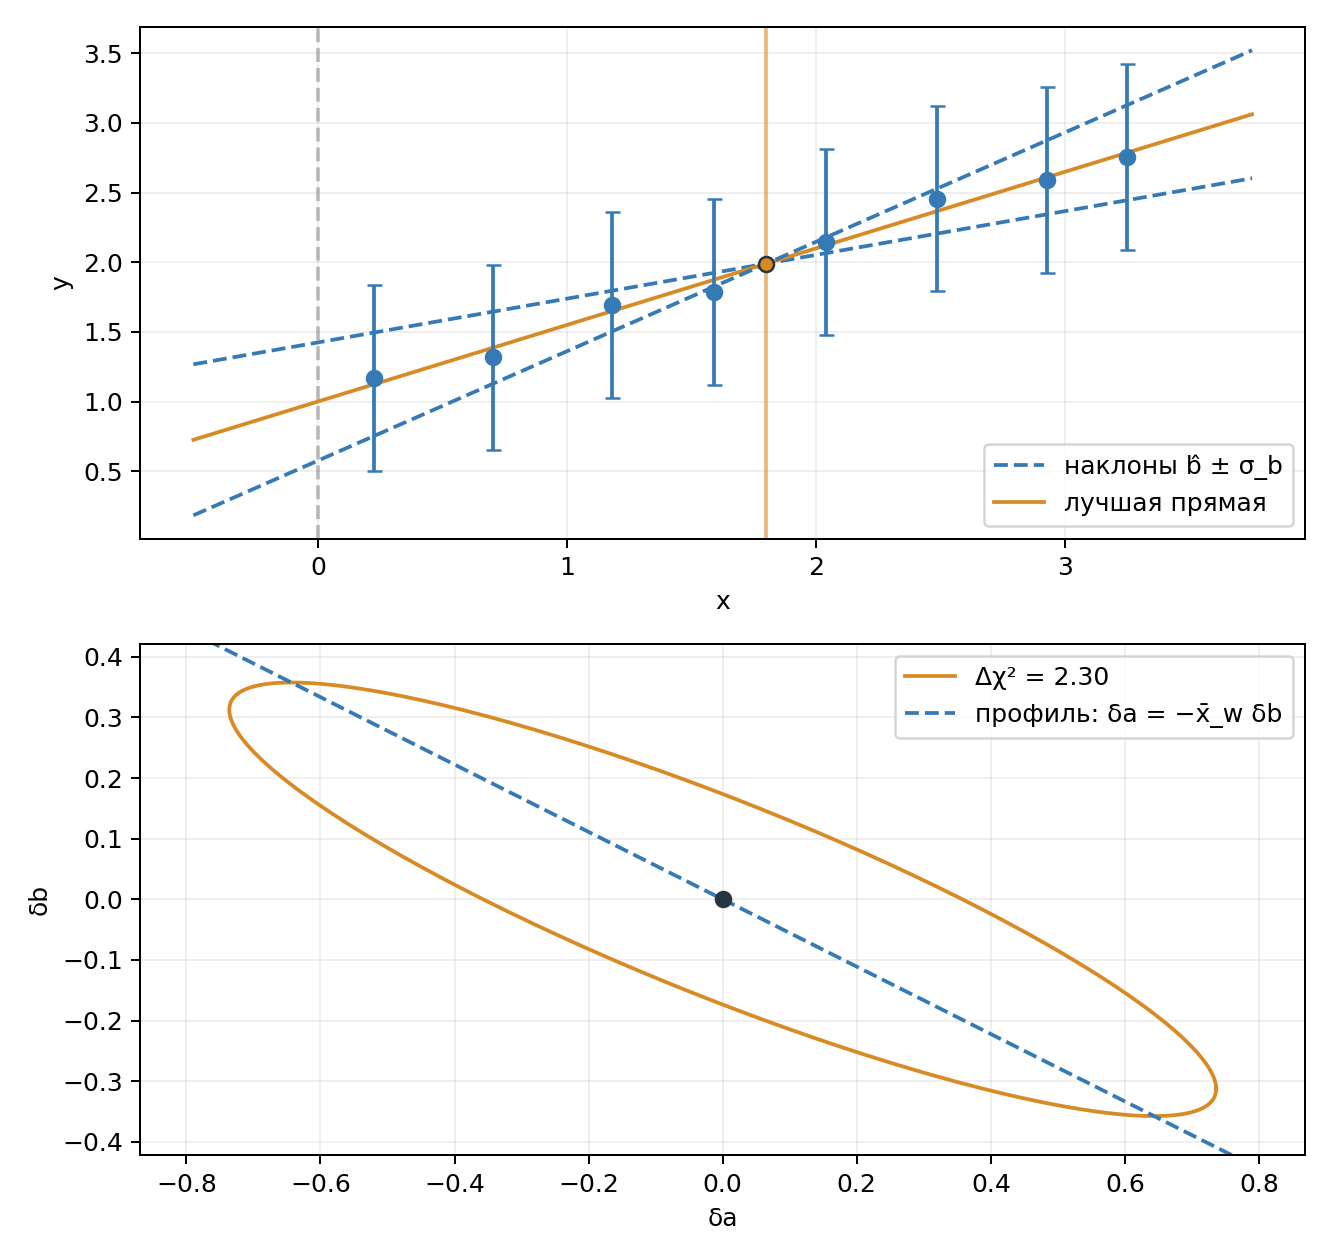
\includegraphics[width=0.74\linewidth,height=\textheight,keepaspectratio,alt={Геометрия корреляции параметров}]{assets/figures/lsq_parameter_geometry.png}

\end{center}

\noindent\begin{minipage}[c]{\dimexpr\linewidth-30mm\relax}

\textbf{Интерактив}. \textbf{Геометрия корреляции параметров}

При \(\bar x_w=1.8\) и \(s_x=1\) корреляция оценок равна \(-0.87\).
Перенос центра к нулю устраняет наклон эллипса. Увеличение разброса
точек уменьшает ошибку наклона прямой.

\end{minipage}\hfill\begin{minipage}[c]{26mm}\centering

\href{https://neutrinohit.github.io/statistical-analysis-course/ru/book/chapters/11_least_squares_linear_fit.html\#interactive-least-squares-parameter-geometry}{
\includegraphics[width=24mm,height=\textheight,keepaspectratio,alt={QR-код интерактива}]{assets/qr/least-squares-parameter-geometry.png}}

\end{minipage}

\end{semanticpdfbox}

\subsection{Центрированная
параметризация}\label{ux446ux435ux43dux442ux440ux438ux440ux43eux432ux430ux43dux43dux430ux44f-ux43fux430ux440ux430ux43cux435ux442ux440ux438ux437ux430ux446ux438ux44f}

Можно сразу измерять \(x\) от центра данных:

\begin{equation}\protect\phantomsection\label{eq-ch11-centered-parameterization}{
x'=x-\bar x_w,
\qquad
f(x)=a'+bx',
\qquad
a'=a+b\bar x_w.
}\end{equation}

Теперь \(\sum_iw_ix_i'=0\), поэтому

\begin{equation}\protect\phantomsection\label{eq-ch11-centered-errors}{
\widehat a'=\bar y_w,
\qquad
\operatorname{Var}(\widehat a')=\frac1S,
\qquad
\operatorname{cov}(\widehat a',\widehat b)=0.
}\end{equation}

Наклон и его ошибка сохранились. Параметр \(a'\) теперь описывает
значение прямой в центре данных. Сама калибровка не изменилась, но её
параметры стали некоррелированными. В гауссовой модели оценки
\(\widehat a'\) и \(\widehat b\) также независимы.

\subsection{Нормальные координаты и
профиль}\label{ux43dux43eux440ux43cux430ux43bux44cux43dux44bux435-ux43aux43eux43eux440ux434ux438ux43dux430ux442ux44b-ux438-ux43fux440ux43eux444ux438ux43bux44c}

В новых координатах квадратичная форма диагональна:

\begin{equation}\protect\phantomsection\label{eq-ch11-normal-coordinates}{
\Delta\chi^2=S(\delta a')^2+Q_x(\delta b)^2
=z_a^2+z_b^2,
\qquad
z_a=\sqrt S\,\delta a',\quad z_b=\sqrt{Q_x}\,\delta b.
}\end{equation}

Мы получили те же нормальные координаты, которые вводили для двумерного
гаусса. Эллипсы превратились в окружности. Здесь преобразование точно во
всей плоскости параметров.

При профилировании по \(a'\) первое слагаемое обращается в нуль.
Остаётся

\begin{equation}\protect\phantomsection\label{eq-ch11-slope-profile}{
\chi^2_{\mathrm p}(b)-\chi^2_{\min}
=Q_x(b-\widehat b)^2
=\frac{(b-\widehat b)^2}{\sigma_b^2}.
}\end{equation}

Поэтому пределы \(\widehat b\pm\sigma_b\) соответствуют росту
профильного \(\chi^2\) на единицу. Это одномерный интервал с покрытием
около \(68.3\%\) в нашей гауссовой модели. Для совместной области двух
параметров с тем же покрытием нужен порог \(\Delta\chi^2=2.30\). Именно
он показан в апплете.

\section{Возвращаемся к
калибровке}\label{ux432ux43eux437ux432ux440ux430ux449ux430ux435ux43cux441ux44f-ux43a-ux43aux430ux43bux438ux431ux440ux43eux432ux43aux435}

Для данных из таблицы \ref{tbl-ch11-calibration-data} все веса равны
\(1/4\) в обратных квадратах канала. Получаем

\begin{equation}\protect\phantomsection\label{eq-ch11-calibration-sums}{
\bar x_w=2\ \text{МэВ},
\qquad
\bar y_w=202\ \text{канала},
\qquad
Q_x=0.5\ \text{МэВ}^2/\text{канал}^2.
}\end{equation}

Из формул \ref{eq-ch11-line-estimates} и
\ref{eq-ch11-errors-from-coordinate-spread} следуют \(\widehat b=100\)
каналов/МэВ и \(\widehat a=2\) канала, \(\sigma_b=\sqrt2\) канала/МэВ и
\(\sigma_a=\sqrt{28/3}\) канала. Ковариация равна \(-4\)
канал\(^2\)/МэВ. Это и даёт результат \ref{eq-ch11-calibration-result} с
корреляцией \(-\sqrt{6/7}\simeq-0.93\).

В центрированной записи та же прямая выглядит проще:

\begin{equation}\protect\phantomsection\label{eq-ch11-centered-calibration}{
\widehat f(x)=202\ \text{канала}
+\left(100\ \frac{\text{каналов}}{\text{МэВ}}\right)(x-2\ \text{МэВ}).
}\end{equation}

Значение в центре равно \(202\pm1.15\) канала и не коррелирует с
наклоном. Ошибка \(1.15\) заметно меньше ошибки свободного члена
\(3.1\): центр данных находится внутри диапазона измерений, а нулевая
энергия --- за его пределами.

\subsection{С какой точностью известна
прямая?}\label{ux441-ux43aux430ux43aux43eux439-ux442ux43eux447ux43dux43eux441ux442ux44cux44e-ux438ux437ux432ux435ux441ux442ux43dux430-ux43fux440ux44fux43cux430ux44f}

В произвольной фиксированной точке \(x\) оценка среднего сигнала равна
\(\widehat f(x)=\widehat a+\widehat bx\). Закон распространения ошибок
даёт

\begin{equation}\protect\phantomsection\label{eq-ch11-fitted-mean-variance}{
\begin{aligned}
\operatorname{Var}[\widehat f(x)]
&=\sigma_a^2+2x\operatorname{cov}(\widehat a,\widehat b)+x^2\sigma_b^2\\
&=\frac1S+\frac{(x-\bar x_w)^2}{Q_x}.
\end{aligned}
}\end{equation}

Это точное равенство: \(\widehat f\) линейна по оценкам. Минимальная
ошибка достигается в центре данных. По мере удаления от центра полоса
вокруг подогнанной прямой расширяется.

Если забыть ковариацию, уже при \(x=2\) МэВ получится дисперсия
\(28/3+8=52/3\) канал\(^2\) вместо \(4/3\) канал\(^2\). Ошибка вырастет
с \(1.15\) до \(4.16\) канала. Сильная корреляция здесь имеет вполне
измеримое последствие.

\subsection{Средний сигнал и новое
измерение}\label{ux441ux440ux435ux434ux43dux438ux439-ux441ux438ux433ux43dux430ux43b-ux438-ux43dux43eux432ux43eux435-ux438ux437ux43cux435ux440ux435ux43dux438ux435}

Теперь проведём ещё одно независимое измерение при фиксированной энергии
\(x_*\), с гауссовой ошибкой известной ширины \(\sigma_*\):

\begin{equation}\protect\phantomsection\label{eq-ch11-prediction-error-variance}{
Y_*=a+bx_*+\varepsilon_*,
\qquad
\operatorname{Var}[Y_*-\widehat f(x_*)]
=\sigma_*^2+\frac1S+\frac{(x_*-\bar x_w)^2}{Q_x}.
}\end{equation}

Первое слагаемое описывает флуктуацию нового измерения. Два остальных
связаны с неопределённостью калибровочной прямой. Поэтому интервал для
нового измерения шире интервала для среднего сигнала.

В центре нашей калибровки средний сигнал известен с ошибкой \(1.15\)
канала. Если новое измерение имеет \(\sigma_*=2\) канала, стандартное
отклонение разности \(Y_*-\widehat f(x_*)\) равно \(\sqrt{4+4/3}=2.31\)
канала. Обе полосы показаны на рисунке \ref{fig-ch11-calibration-bands}.

\begin{figure}[H]

\centering{

\pandocbounded{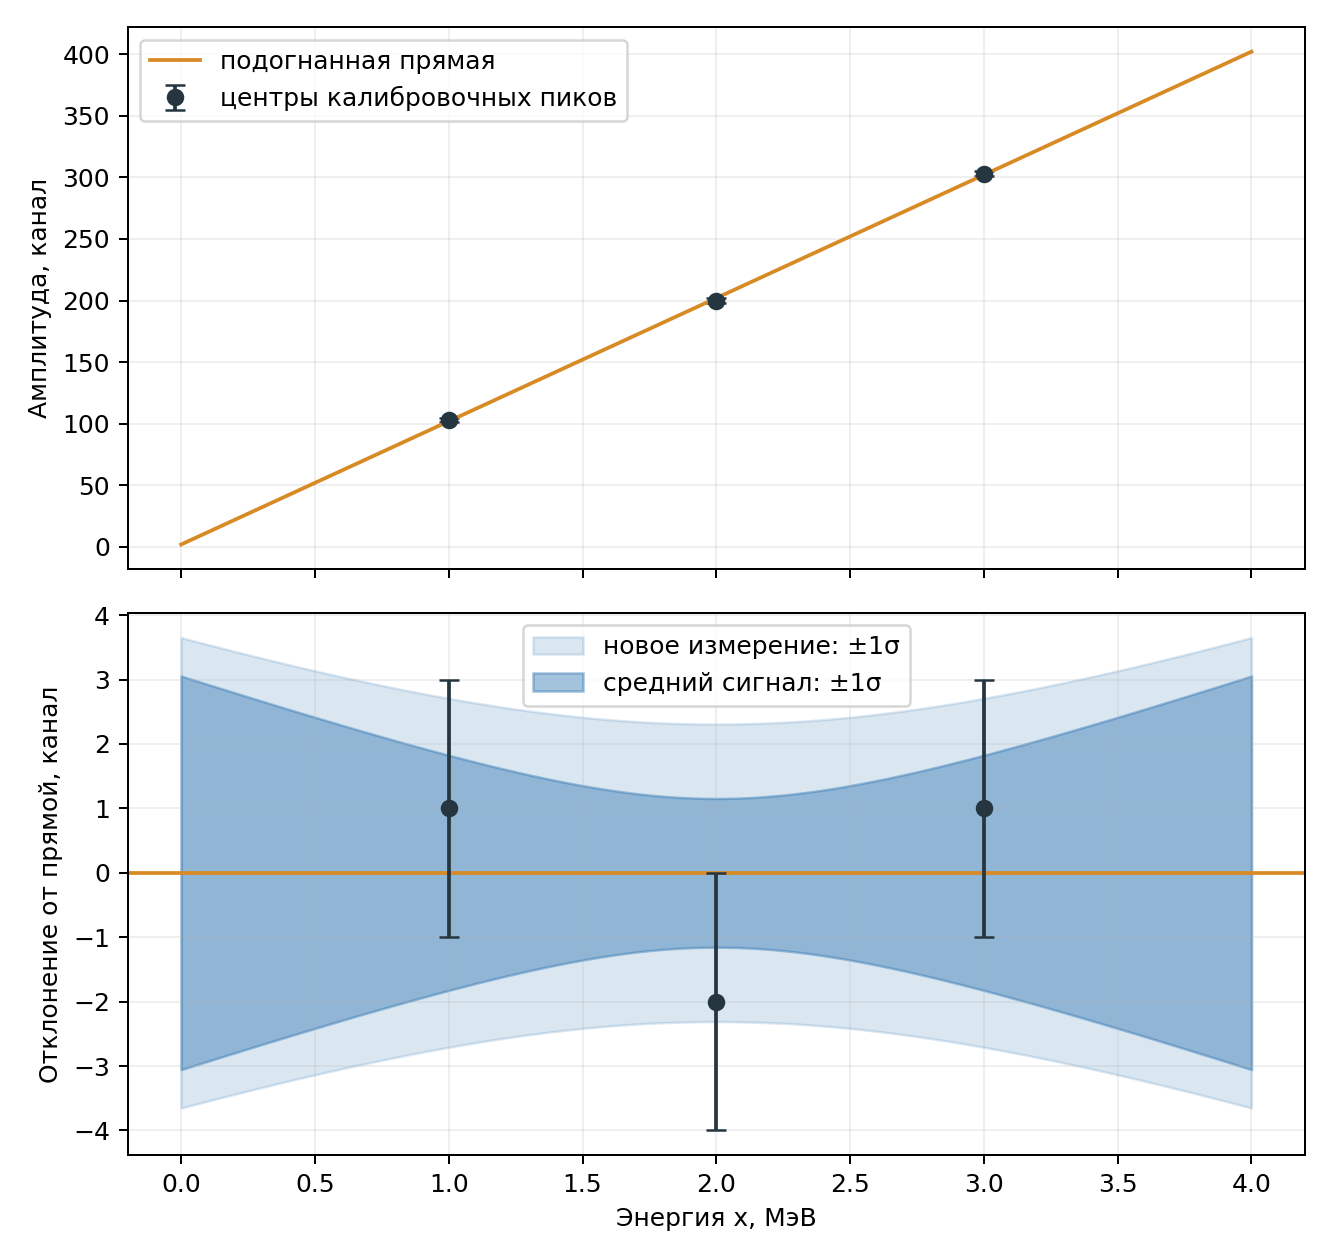
\includegraphics[keepaspectratio]{chapters/../assets/figures/lsq_calibration_bands.png}}

}

\caption{\label{fig-ch11-calibration-bands}Учебная калибровка из
таблицы: точки с ошибками и подогнанная прямая. На нижнем графике из
каждой величины вычтена подогнанная прямая, чтобы различить полосы.
Узкая полоса соответствует одной стандартной ошибке среднего сигнала;
широкая учитывает также ошибку нового независимого измерения
\(\sigma_*=2\) канала.}

\end{figure}%

Границы обеих полос имеют точечное покрытие около \(68.3\%\) при каждом
заранее фиксированном \(x\). Утверждение о всей кривой сразу требует
одновременной доверительной полосы с другим порогом. Кроме того, за
пределами калибровочного диапазона эти формулы учитывают лишь ошибки
параметров прямой. Возможную нелинейность реального отклика они не
описывают.

\section{Что остаётся после
подгонки}\label{ux447ux442ux43e-ux43eux441ux442ux430ux451ux442ux441ux44f-ux43fux43eux441ux43bux435-ux43fux43eux434ux433ux43eux43dux43aux438}

Остатки при найденных параметрах равны

\begin{equation}\protect\phantomsection\label{eq-ch11-fitted-residuals}{
r_i=y_i-\widehat a-\widehat bx_i,
\qquad
u_i=\frac{r_i}{\sigma_i}.
}\end{equation}

Величины \(u_i\) позволяют сравнивать отклонения точек с разными
ошибками. Однако считать их независимой выборкой из \(\mathcal N(0,1)\)
нельзя. Прямая уже подстроилась под те же точки. Из нормальных уравнений
следуют два ограничения:

\begin{equation}\protect\phantomsection\label{eq-ch11-residual-constraints}{
\sum_iw_i r_i=0,
\qquad
\sum_iw_ix_i r_i=0.
}\end{equation}

Изменение одной точки меняет прямую и тем самым остатки остальных точек.
Найдём эту связь явно.

\subsection{Матрица
влияния}\label{ux43cux430ux442ux440ux438ux446ux430-ux432ux43bux438ux44fux43dux438ux44f}

Разделим данные и модель в каждой строке на \(\sigma_i\):

\begin{equation}\protect\phantomsection\label{eq-ch11-standardized-design}{
z_i=\frac{y_i}{\sigma_i},
\qquad
B_{i1}=\frac1{\sigma_i},
\qquad
B_{i2}=\frac{x_i}{\sigma_i}.
}\end{equation}

Матрица \(B\) имеет \(N\) строк и два столбца. Ошибки вектора
\(\mathbf z\) независимы и имеют единичную дисперсию. Нормальные
уравнения теперь записываются как
\(B^{\mathsf T}B\widehat{\boldsymbol\beta}=B^{\mathsf T}\mathbf z\).
Значения подогнанной модели в этих координатах равны

\begin{equation}\protect\phantomsection\label{eq-ch11-hat-matrix}{
\widehat{\mathbf z}=H\mathbf z,
\qquad
H=B(B^{\mathsf T}B)^{-1}B^{\mathsf T}.
}\end{equation}

Матрица \(H\) называется \textbf{матрицей влияния}. Она симметрична и
удовлетворяет \(H^2=H\): если ещё раз подогнать уже лежащие на прямой
значения, они не изменятся. Вектор нормированных остатков равен
\(\mathbf u=(I-H)\mathbf z\), где \(I\) --- единичная матрица. Поэтому

\begin{equation}\protect\phantomsection\label{eq-ch11-residual-covariance}{
\operatorname{Cov}(\mathbf u)
=(I-H)(I-H)^{\mathsf T}=I-H.
}\end{equation}

В частности,

\begin{equation}\protect\phantomsection\label{eq-ch11-leverage}{
\operatorname{Var}(u_i)=1-h_{ii},
\qquad
h_{ii}=w_i\left[\frac1S+\frac{(x_i-\bar x_w)^2}{Q_x}\right].
}\end{equation}

Точка с большим \(h_{ii}\) сильнее подтягивает к себе прямую, поэтому её
остаток имеет меньшую дисперсию. При прочих равных большое влияние имеют
точки далеко от центра \(x\). Малый остаток такой точки сам по себе ещё
не означает, что с измерением всё в порядке.

Для известной дисперсии ошибки и \(h_{ii}<1\) величина
\(u_i/\sqrt{1-h_{ii}}\) имеет единичную дисперсию, а в нашей гауссовой
модели и стандартное нормальное распределение. Эта нормировка не
устраняет корреляций между разными остатками.

\subsection{\texorpdfstring{Почему остаётся \(N-2\) степеней
свободы}{Почему остаётся N-2 степеней свободы}}\label{ux43fux43eux447ux435ux43cux443-ux43eux441ux442ux430ux451ux442ux441ux44f-n-2-ux441ux442ux435ux43fux435ux43dux435ux439-ux441ux432ux43eux431ux43eux434ux44b}

Матрица \(H\) проектирует данные на двумерное пространство моделей,
заданное двумя столбцами \(B\). У неё два собственных значения \(1\),
остальные равны \(0\), и \(\operatorname{tr}H=2\). Для остатков остаётся
\(N-2\) независимых направлений. При верной линейной модели и известных
гауссовых ошибках

\begin{equation}\protect\phantomsection\label{eq-ch11-residual-degrees-of-freedom}{
\chi^2_{\min}=\mathbf u^{\mathsf T}\mathbf u
\sim\chi^2_{N-2},
\qquad
\mathbb E[\chi^2_{\min}]=N-2.
}\end{equation}

Распределение справа обозначено тем же символом \(\chi^2\), что и
функция, которую мы минимизировали. Здесь \(N>2\). Для нашей калибровки
остатки равны \(1,-2,1\) канала, поэтому \(\chi^2_{\min}=1.5\) при одной
степени свободы. Из одного такого числа нельзя заключить, что модель
детектора верна. Формальную проверку согласия разберём в главе 13.

Если ошибки всех точек имеют одинаковую, но неизвестную дисперсию
\(\sigma^2\), её можно оценить по остаткам:

\begin{equation}\protect\phantomsection\label{eq-ch11-residual-scale-estimator}{
s^2=\frac1{N-2}\sum_i r_i^2,
\qquad
\mathbb E[s^2]=\sigma^2.
}\end{equation}

Для интервалов тогда требуется учитывать случайность \(s\), что приводит
к распределению Стьюдента. В нашей основной задаче все \(\sigma_i\)
заданы заранее. Перемасштабировать их до \(\chi^2_{\min}/(N-2)=1\)
оснований нет.

\section{Остатки и выбросы}\label{interactive-least-squares-outlier}

Сгенерируем \(16\) точек около прямой \(y=1+0.8x\) с независимыми
гауссовыми ошибками. Обе координаты здесь безразмерные. В апплете можно
изменить масштаб ошибок и добавить сдвиг \(d\) к одной отмеченной точке.
При изменении сдвига остальные точки сохраняются. Кнопка «Новые данные»
меняет всю случайную выборку.

\begin{semanticpdfbox}[breakable=false]

\begin{center}

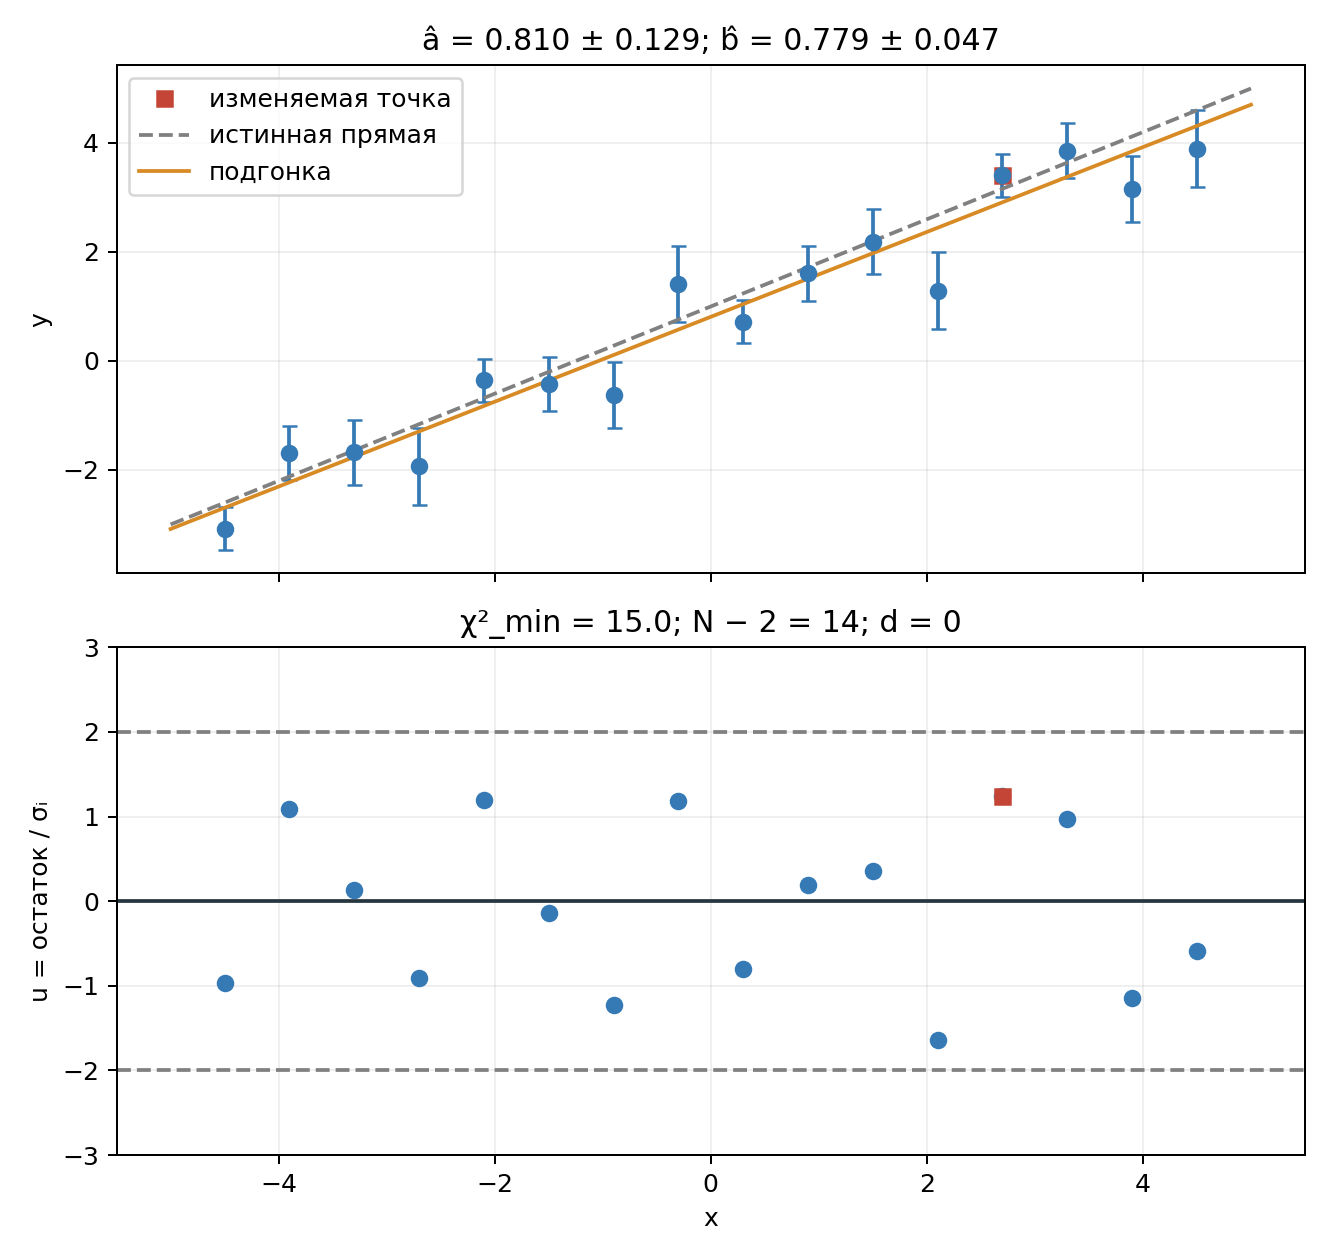
\includegraphics[width=0.74\linewidth,height=\textheight,keepaspectratio,alt={Прямая, остатки и выброс}]{assets/figures/lsq_fit_no_outlier.png}

\end{center}

\noindent\begin{minipage}[c]{\dimexpr\linewidth-30mm\relax}

\textbf{Интерактив}. \textbf{Прямая, остатки и выброс}

Подгонка \(16\) псевдоизмерений при масштабе ошибок \(0.55\) и без
дополнительного сдвига. Пунктиром показана истинная прямая, сплошной
линией --- результат подгонки. Нижний график содержит остатки, делённые
на ошибки точек.

\end{minipage}\hfill\begin{minipage}[c]{26mm}\centering

\href{https://neutrinohit.github.io/statistical-analysis-course/ru/book/chapters/11_least_squares_linear_fit.html\#interactive-least-squares-outlier}{
\includegraphics[width=24mm,height=\textheight,keepaspectratio,alt={QR-код интерактива}]{assets/qr/least-squares-outlier.png}}

\end{minipage}

\end{semanticpdfbox}

На рисунке \ref{fig-least-squares-outlier} к той же выборке добавлен
сдвиг \(d=4\) в одной точке. Её заявленная ошибка не изменилась.
Подгонка учитывает эту точку с прежним весом, и прямая смещается.

\begin{figure}[H]

\centering{

\pandocbounded{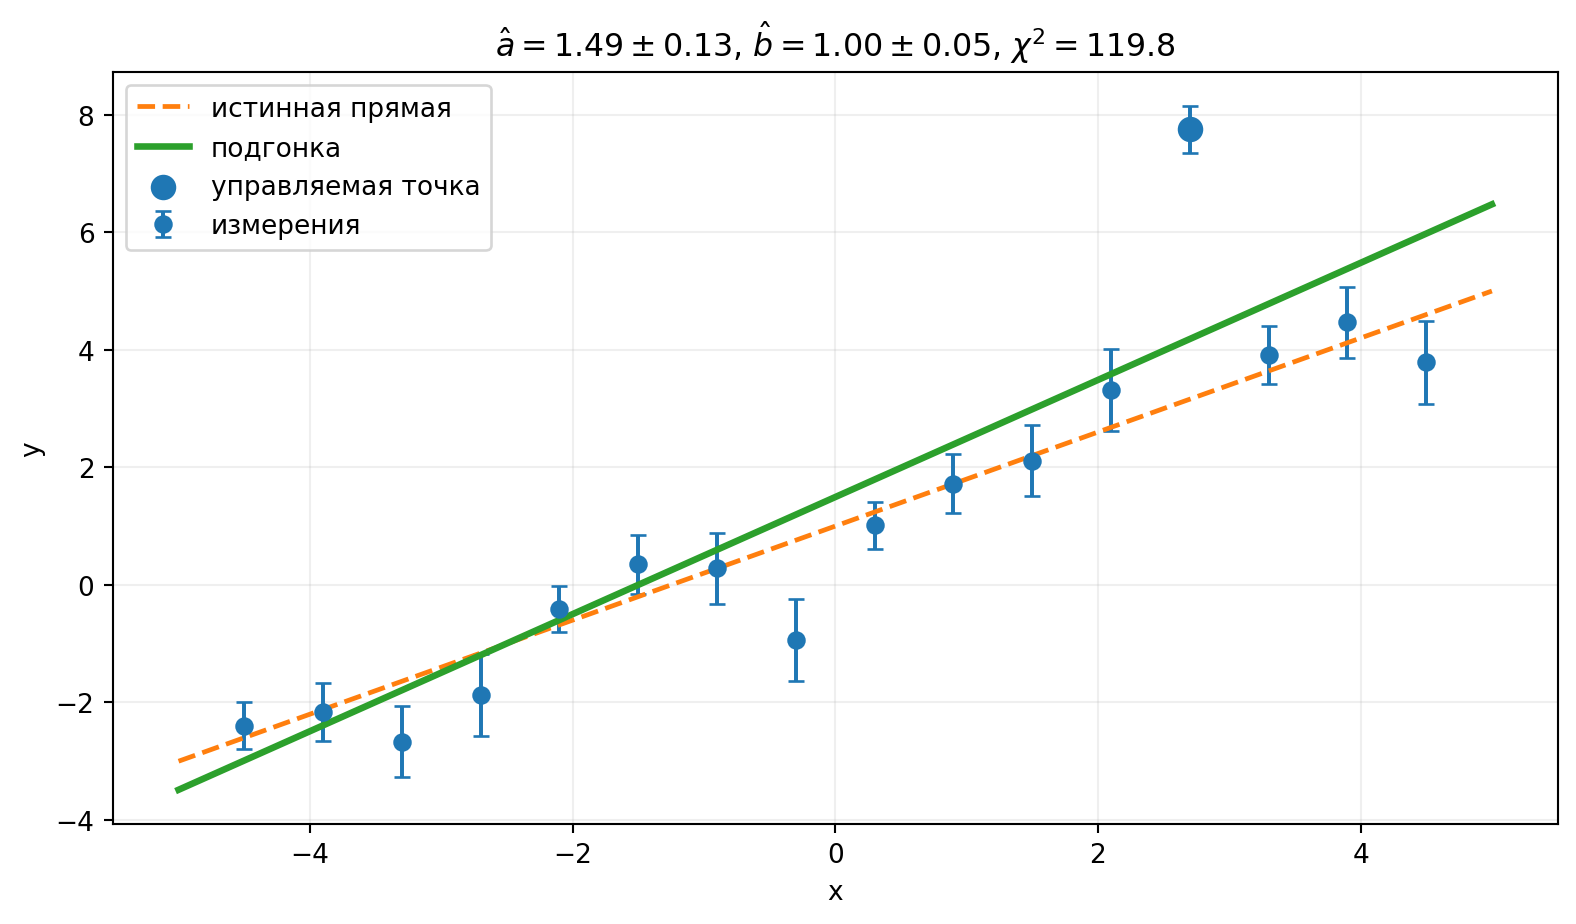
\includegraphics[keepaspectratio]{chapters/../assets/figures/lsq_fit_with_outlier.png}}

}

\caption{\label{fig-least-squares-outlier}Те же псевдоизмерения после
сдвига отмеченной точки на \(d=4\). Пунктирная прямая задаёт исходную
модель, сплошная получена из подгонки. Сдвиг одной точки изменил и её
собственный остаток, и остатки остальных измерений.}

\end{figure}%

Этот эффект можно вычислить без повторной минимизации. Если заменить
\(y_j\) на \(y_j+d\) при неизменных координатах и весах, то

\begin{equation}\protect\phantomsection\label{eq-ch11-single-point-shift}{
\delta\widehat b=\frac{w_j(x_j-\bar x_w)}{Q_x}\,d,
\qquad
\delta\widehat a=\frac{w_j}{S}\,d-\bar x_w\delta\widehat b.
}\end{equation}

Смещение наклона растёт линейно с \(d\) и с расстоянием точки от центра.
Обычный МНК не ограничивает влияние сколь угодно большого отклонения.

Что делать, если такая точка встретилась в эксперименте? Нужно проверить
причину: сбой электроники, неверную ошибку измерения, примесь другого
процесса, насыщение детектора или недостаточность самой модели. Удаление
точки требует физического основания и явно описанного правила отбора.
Если большие отклонения составляют часть распределения ошибок, это
распределение следует включить в правдоподобие.

На графике остатков полезно смотреть также на согласованное поведение
многих точек. Изгиб может указывать на нелинейность отклика. Рост
разброса с \(x\) может означать, что зависимость ошибок от энергии
описана неверно. Такой график помогает поставить вопрос к модели; сам по
себе он ещё не выбирает причину отклонения.

\begin{bookchaptersummary}[Итоги главы]

\begin{itemize}
\tightlist
\item
  Для независимых гауссовых измерений с известными, не зависящими от
  параметров дисперсиями МНК совпадает с методом максимального
  правдоподобия.
\item
  Подгонка прямой сводится к двум нормальным уравнениям. Ковариация
  оценок определяется координатами точек и их ошибками.
\item
  Центрирование координаты устраняет ковариацию наклона и значения
  прямой в центре данных. При вычислении ошибки кривой в исходных
  параметрах ковариационный член необходимо сохранять.
\item
  После подгонки остатки связаны между собой и имеют уменьшенные
  дисперсии. Их структура и влияние отдельных точек позволяют проверять
  описание измерений.
\end{itemize}

\end{bookchaptersummary}

\section{Задачи}\label{ux437ux430ux434ux430ux447ux438-10}

\begin{semanticpdfbox}[colback=BookCoralSoft,borderline west={1.2mm}{0pt}{BookCoral},breakable=false]

\noindent{\sffamily\bfseries\fontsize{11.2}{13.5}\selectfont Задача 1. Среднее как результат МНК}\par\nopagebreak[4]\vspace{1.2mm}

Имеются независимые измерения одной величины: \[
Y_i\sim\mathrm N(\mu,\sigma_i^2).
\]

Все \(\sigma_i>0\) известны и не зависят от \(\mu\).

\begin{enumerate}
\def\labelenumi{\arabic{enumi}.}
\tightlist
\item
  Запишите функцию \(\chi^2(\mu)\).
\item
  Найдите её минимум.
\item
  Покажите, что полученная оценка является взвешенным средним.
\item
  Найдите дисперсию этой оценки.
\item
  Рассмотрите частный случай одинаковых \(\sigma_i\).
\end{enumerate}

\end{semanticpdfbox}

\begin{semanticpdfbox}[colback=BookCoralSoft,borderline west={1.2mm}{0pt}{BookCoral},breakable=false]

\noindent{\sffamily\bfseries\fontsize{11.2}{13.5}\selectfont Задача 2. Аналитическая подгонка прямой}\par\nopagebreak[4]\vspace{1.2mm}

Для данных \((x_i,y_i,\sigma_i)\) рассматривается модель \[
y=a+bx.
\]

Координаты \(x_i\) известны точно, ошибки по \(y\) независимы и
гауссовы, их стандартные отклонения \(\sigma_i>0\) известны. Среди
\(x_i\) есть хотя бы два различных значения.

\begin{enumerate}
\def\labelenumi{\arabic{enumi}.}
\tightlist
\item
  Выведите нормальные уравнения.
\item
  Получите аналитические формулы для \(\widehat a\) и \(\widehat b\).
\item
  Выведите ковариационную матрицу параметров.
\item
  Покажите, что центрирование \(x_i\) около взвешенного среднего
  устраняет ковариацию параметров.
\item
  Проверьте формулы численно на искусственной выборке.
\end{enumerate}

\end{semanticpdfbox}

\begin{semanticpdfbox}[colback=BookCoralSoft,borderline west={1.2mm}{0pt}{BookCoral},breakable=false]

\noindent{\sffamily\bfseries\fontsize{11.2}{13.5}\selectfont Задача 3. Ошибка подогнанной кривой}\par\nopagebreak[4]\vspace{1.2mm}

Три независимых гауссовых измерения при точно известных энергиях
\(x=(1,2,3)\) МэВ дали положения пиков \(y=(103,200,303)\) канала.
Ошибка каждого положения равна \(2\) каналам. Для модели \(f(x)=a+bx\)
найдите:

\begin{enumerate}
\def\labelenumi{\arabic{enumi}.}
\tightlist
\item
  дисперсию оценки среднего \(\widehat y(x)=\widehat a+\widehat bx\);
\item
  точку, в которой эта дисперсия минимальна;
\item
  дисперсию разности \(Y_*-\widehat y(x_*)\) для нового независимого
  измерения при фиксированном \(x_*\) с известной ошибкой \(\sigma_*\);
\item
  различие между полосой среднего сигнала и полосой для нового
  измерения.
\end{enumerate}

Постройте обе полосы для этих данных при \(\sigma_*=2\) канала.
Объясните, почему точечное покрытие не означает покрытия всей кривой
сразу.

\end{semanticpdfbox}

\begin{semanticpdfbox}[colback=BookCoralSoft,borderline west={1.2mm}{0pt}{BookCoral},breakable=false]

\noindent{\sffamily\bfseries\fontsize{11.2}{13.5}\selectfont Задача 4. Остатки и диагональные элементы матрицы влияния}\par\nopagebreak[4]\vspace{1.2mm}

Пусть \(N>2\), \(y_i=a+bx_i+\varepsilon_i\), а \(\varepsilon_i\)
независимы, имеют нулевые средние и одну известную дисперсию
\(\sigma^2\). Координаты \(x_i\) фиксированы и не все одинаковы. В этом
случае \(\widehat{\mathbf y}=H\mathbf y\), где
\(H=X(X^{\mathsf T}X)^{-1}X^{\mathsf T}\), \(X_{i1}=1\), \(X_{i2}=x_i\).
Обозначьте остатки через \(\mathbf r=\mathbf y-\widehat{\mathbf y}\), а
единичную матрицу через \(I\).

\begin{enumerate}
\def\labelenumi{\arabic{enumi}.}
\tightlist
\item
  покажите, что \(H^2=H\);
\item
  покажите, что \(\operatorname{tr}H=2\);
\item
  выведите ковариацию остатков \[
  \operatorname{Cov}(\mathbf r)=\sigma^2(I-H);
  \]
\item
  найдите диагональные элементы \(h_{ii}\), характеризующие влияние
  точек при подгонке прямой;
\item
  добавьте одну далёкую по \(x\) точку и исследуйте её влияние.
\end{enumerate}

\end{semanticpdfbox}

\begin{semanticpdfbox}[colback=BookCoralSoft,borderline west={1.2mm}{0pt}{BookCoral},breakable=false]

\noindent{\sffamily\bfseries\fontsize{11.2}{13.5}\selectfont Задача 5. Влияние одной точки}\par\nopagebreak[4]\vspace{1.2mm}

Сгенерируйте \(16\) независимых гауссовых измерений около прямой
\(y=1+0.8x\) при \(x_i=-4.5+9(i-1)/15\), \(i=1,\ldots,16\), и известных
одинаковых ошибках \(\sigma_i=0.55\). Зафиксируйте начальное состояние
генератора.

\begin{enumerate}
\def\labelenumi{\arabic{enumi}.}
\tightlist
\item
  Выполните подгонку обычным методом наименьших квадратов.
\item
  Добавьте к одной точке сдвиг \(d\), сохранив её заявленную ошибку.
  Выведите изменения \(\widehat a\) и \(\widehat b\) из нормальных
  уравнений.
\item
  Меняйте \(d\) от \(-4\) до \(6\) и сравните формулы с повторной
  подгонкой.
\item
  Повторите опыт для точки вблизи центра и для крайней точки. Сравните
  влияние на наклон и остатки.
\item
  Проверьте, меняется ли вычисленная ковариация параметров при этих
  сдвигах. Объясните, почему неизменная ошибка параметра не гарантирует
  отсутствия смещения из-за испорченного измерения.
\end{enumerate}

\end{semanticpdfbox}

\section*{Литература}\label{ux43bux438ux442ux435ux440ux430ux442ux443ux440ux430-10}
\addcontentsline{toc}{section}{Литература}

\markright{Литература}

\protect\phantomsection\label{refs}
\begin{CSLReferences}{0}{0}
\bibitem[\citeproctext]{ref-cowan1998}
{[}1{]} Cowan, G. \emph{Statistical Data Analysis}. Oxford University
Press. 1998.

\end{CSLReferences}

\chapter{χ²-интервалы и систематические
неопределённости}\label{ux3c7uxb2-ux438ux43dux442ux435ux440ux432ux430ux43bux44b-ux438-ux441ux438ux441ux442ux435ux43cux430ux442ux438ux447ux435ux441ux43aux438ux435-ux43dux435ux43eux43fux440ux435ux434ux435ux43bux451ux43dux43dux43eux441ux442ux438}

\bookchapteropeningcontents

\begin{bookchapteropening}[Аннотация]

В прошлой главе ошибки измерений были независимы. Теперь включим в
подгонку корреляции и неизвестные калибровочные параметры. Разберём, как
из формы χ² получают ошибки и интервалы, откуда берутся штрафные члены и
когда профилирование можно выполнить аналитически. Пример с общей
нормировкой покажет, почему при построении ковариации нужно различать
данные и модель.

\end{bookchapteropening}

\section{Физическая задача: два измерения с общей
нормировкой}\label{ux444ux438ux437ux438ux447ux435ux441ux43aux430ux44f-ux437ux430ux434ux430ux447ux430-ux434ux432ux430-ux438ux437ux43cux435ux440ux435ux43dux438ux44f-ux441-ux43eux431ux449ux435ux439-ux43dux43eux440ux43cux438ux440ux43eux432ux43aux43eux439}

Пусть сечение процесса измерено по двум независимым наборам событий. Оба
результата используют одну калибровку светимости, поэтому часть их
ошибки общая. Возьмём числа из примера Д'Агостини {[}1{]} и для
определённости будем измерять сечение в пб:

\begin{equation}\protect\phantomsection\label{eq-ch12-normalization-data}{
y_1=(8.00\pm0.16)\ \text{пб},
\qquad
y_2=(8.50\pm0.17)\ \text{пб}.
}\end{equation}

Выписанные ошибки относятся к независимой части. Кроме них имеется общая
относительная неопределённость нормировки \(f_N=0.10\). В расчёте
считаем независимые ошибки гауссовыми, а их стандартные отклонения
\(s_1=0.16\) пб и \(s_2=0.17\) пб --- заданными числами. Они не меняются
вместе с пробным сечением. Числа относятся к учебной модели.

Как объединить эти два числа? Если пока забыть про нормировку,
взвешенное среднее равно \(8.235\) пб. После учёта общей нормировки наша
модель даст

\begin{equation}\protect\phantomsection\label{eq-ch12-normalization-first-result}{
\widehat\mu=(8.235\pm0.832)\ \text{пб},
}\end{equation}

где ошибка найдена по кривизне в минимуме. Но есть весьма правдоподобный
способ записать ковариационную матрицу, который вместо этого приводит к
\(7.87\pm0.81\) пб. Центральное значение оказалось ниже обеих точек.

Почему так получилось? И какое усреднение описывает наш эксперимент? Для
ответа нужно проследить, как общая калибровка входит в предсказание.
Начнём с МНК для коррелированных измерений.

\section{Общий случай с ковариационной
матрицей}\label{ux43eux431ux449ux438ux439-ux441ux43bux443ux447ux430ux439-ux441-ux43aux43eux432ux430ux440ux438ux430ux446ux438ux43eux43dux43dux43eux439-ux43cux430ux442ux440ux438ux446ux435ux439}

Соберём \(N\) результатов в вектор \(\mathbf y\), а их математические
ожидания --- в вектор \(\boldsymbol\lambda(\boldsymbol\theta)\).
Параметры модели обозначены \(\boldsymbol\theta\). Пусть данные имеют
многомерное гауссово распределение с известной положительно определённой
ковариацией \(V_y\):

\begin{equation}\protect\phantomsection\label{eq-ch12-multivariate-data-model}{
\mathbf Y\sim\mathcal N\bigl(\boldsymbol\lambda(\boldsymbol\theta),V_y\bigr).
}\end{equation}

При фиксированной \(V_y\) логарифм правдоподобия с точностью до
постоянного слагаемого определяется квадратичной формой {[}2{]}

\begin{equation}\protect\phantomsection\label{eq-correlated-least-squares}{
\chi^2(\boldsymbol\theta)
=(\mathbf y-\boldsymbol\lambda)^{\mathsf T}V_y^{-1}
(\mathbf y-\boldsymbol\lambda).
}\end{equation}

В главе о двумерном гауссе мы уже встречали такую меру отклонения от
центра. Теперь центром служит модель, которую мы подгоняем. Если \(V_y\)
диагональна, формула \ref{eq-correlated-least-squares} превращается в
знакомую сумму \(\sum_i r_i^2/\sigma_i^2\).

При корреляциях отдельные остатки нельзя рассматривать независимо.
Например, общая ошибка шкалы может сдвинуть сразу несколько точек в одну
сторону. Вероятность такого согласованного отклонения отличается от
вероятности нескольких независимых сдвигов того же размера.
Внедиагональные элементы \(V_y\) как раз учитывают эту связь.

Если ковариация самой модели данных зависит от параметров, из нормировки
гауссовой плотности появляется ещё одно слагаемое:

\begin{equation}\protect\phantomsection\label{eq-ch12-gaussian-variable-covariance}{
-2\ln L(\boldsymbol\theta)
=\mathbf r^{\mathsf T}V_y(\boldsymbol\theta)^{-1}\mathbf r
+\ln\det V_y(\boldsymbol\theta)+\mathrm{const},
\qquad
\mathbf r=\mathbf y-\boldsymbol\lambda(\boldsymbol\theta).
}\end{equation}

Отбрасывать меняющийся определитель нельзя. Ниже появится внешне похожая
матрица после профилирования. Мы отдельно выясним, почему к ней это
правило автоматически не переносится.

\subsection{Несколько линейных
параметров}\label{ux43dux435ux441ux43aux43eux43bux44cux43aux43e-ux43bux438ux43dux435ux439ux43dux44bux445-ux43fux430ux440ux430ux43cux435ux442ux440ux43eux432}

Пусть модель линейна по \(p\) параметрам:

\begin{equation}\protect\phantomsection\label{eq-ch12-linear-model}{
\boldsymbol\lambda=X\boldsymbol\theta,
\qquad X\in\mathbb R^{N\times p}.
}\end{equation}

Столбцы известной матрицы \(X\) задают, как каждый параметр меняет
предсказания. Для прямой это столбцы \(1\) и \(x_i\). Приравнивая
производные \(\chi^2\) к нулю, получаем нормальные уравнения

\begin{equation}\protect\phantomsection\label{eq-ch12-general-normal-equations}{
X^{\mathsf T}V_y^{-1}X\widehat{\boldsymbol\theta}
=X^{\mathsf T}V_y^{-1}\mathbf y.
}\end{equation}

Если столбцы \(X\) линейно независимы, решение единственно:

\begin{equation}\protect\phantomsection\label{eq-ch12-linear-estimate-covariance}{
\widehat{\boldsymbol\theta}
=(X^{\mathsf T}V_y^{-1}X)^{-1}X^{\mathsf T}V_y^{-1}\mathbf y,
\qquad
V_\theta=(X^{\mathsf T}V_y^{-1}X)^{-1}.
}\end{equation}

Проверка ковариации повторяет вывод для прямой. Оценка имеет вид
\(\widehat{\boldsymbol\theta}=B\mathbf Y\), где \(BX=I\). Поэтому
\(\mathbb E[\widehat{\boldsymbol\theta}]=\boldsymbol\theta\) и
\(\operatorname{Cov}(\widehat{\boldsymbol\theta})=BV_yB^{\mathsf T}=V_\theta\).
Для этих двух равенств достаточно верных первых двух моментов данных.
Гауссова модель дополнительно даёт гауссово распределение оценок.

\subsection{Ошибка по
кривизне}\label{ux43eux448ux438ux431ux43aux430-ux43fux43e-ux43aux440ux438ux432ux438ux437ux43dux435}

В нелинейной модели точного решения обычно нет. Найдём минимум численно
и разложим функцию около него. Обозначим через \(K\) половину матрицы
вторых производных:

\begin{equation}\protect\phantomsection\label{eq-ch12-curvature-covariance}{
\begin{aligned}
\chi^2(\boldsymbol\theta)
&\simeq\chi^2_{\min}
+(\boldsymbol\theta-\widehat{\boldsymbol\theta})^{\mathsf T}
K(\boldsymbol\theta-\widehat{\boldsymbol\theta}),\\
K_{ij}&=\frac12\left.
\frac{\partial^2\chi^2}{\partial\theta_i\partial\theta_j}
\right|_{\widehat{\boldsymbol\theta}},
\qquad V_\theta\simeq K^{-1}.
\end{aligned}
}\end{equation}

Множитель \(1/2\) приходит из формулы Тейлора. Его можно проверить на
одной параболе: вторая производная
\((\theta-\widehat\theta)^2/\sigma^2\) равна \(2/\sigma^2\). Если
обратить её без двойки, дисперсия получится вдвое меньше.

Для линейной модели с известной ковариацией формула точна. В общем
случае \(K^{-1}\) даёт локальную оценку ковариации. Она требует
изолированного внутреннего минимума с положительной кривизной и
достаточно близкой к квадратичной формы правдоподобия в интересующей
области. Узкий минимум ещё нужно найти среди всех остальных минимумов,
если они есть.

\section{\texorpdfstring{Интервалы из формы
\(\chi^2\)}{Интервалы из формы \textbackslash chi\^{}2}}\label{ux438ux43dux442ux435ux440ux432ux430ux43bux44b-ux438ux437-ux444ux43eux440ux43cux44b-chi2}

\subsection{Один параметр}\label{interactive-least-squares-delta-chi2}

Для одного параметра квадратичная форма записывается совсем просто:

\begin{equation}\protect\phantomsection\label{eq-ch12-one-parameter-parabola}{
\Delta\chi^2(\theta)
=\chi^2(\theta)-\chi^2_{\min}
\simeq\frac{(\theta-\widehat\theta)^2}{\sigma_\theta^2}.
}\end{equation}

Отступим от минимума на одну стандартную ошибку. Значение \(\chi^2\)
вырастет на единицу:

\begin{equation}\protect\phantomsection\label{eq-ch12-one-sigma-crossings}{
\Delta\chi^2(\widehat\theta\pm\sigma_\theta)=1.
}\end{equation}

Если вместе с \(\theta\) подгоняются другие неизвестные параметры, здесь
нужна \textbf{профильная} функция: при каждом пробном \(\theta\)
остальные параметры подбираются заново. Сечение с зафиксированными
параметрами может оказаться значительно уже. Мы видели это на
коррелированной паре в главе 10.

В апплете меняются стандартная ошибка \(\sigma_\theta\) и уровень
отсечения \(c\). Обе координаты безразмерные. Пересечения удовлетворяют
\(\theta-\widehat\theta=\pm\sqrt c\,\sigma_\theta\). Попробуйте поднять
уровень с \(1\) до \(4\): интервал расширится вдвое.

\begin{semanticpdfbox}[breakable=false]

\begin{center}

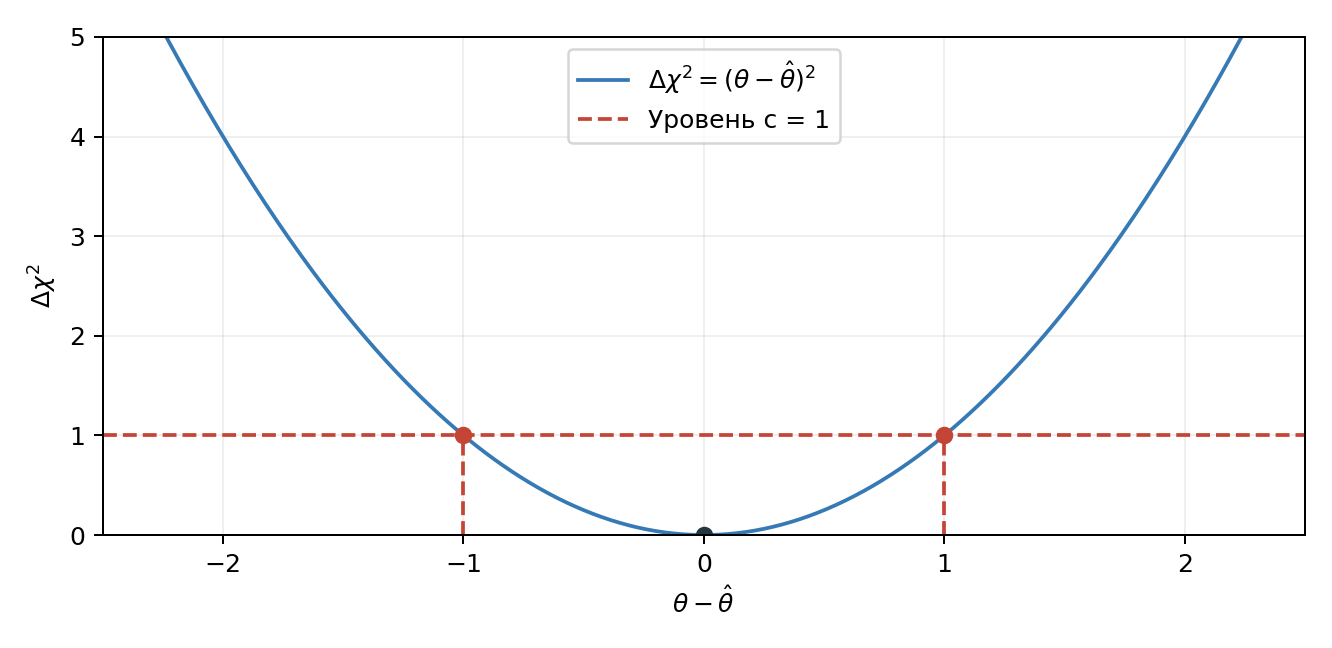
\includegraphics[width=0.74\linewidth,height=\textheight,keepaspectratio,alt={Интервал по пересечению с уровнем χ²}]{assets/figures/lsq_delta_chi2_one_sigma.png}

\end{center}

\noindent\begin{minipage}[c]{\dimexpr\linewidth-30mm\relax}

\textbf{Интерактив}. \textbf{Интервал по пересечению с уровнем χ²}

При \(\sigma_\theta=1\) и \(c=1\) границы лежат при
\(\theta-\widehat\theta=\pm1\). Пунктир задаёт уровень отсечения,
сплошная кривая показывает \(\Delta\chi^2\).

\end{minipage}\hfill\begin{minipage}[c]{26mm}\centering

\href{https://neutrinohit.github.io/statistical-analysis-course/ru/book/chapters/12_least_squares_systematics.html\#interactive-least-squares-delta-chi2}{
\includegraphics[width=24mm,height=\textheight,keepaspectratio,alt={QR-код интерактива}]{assets/qr/least-squares-delta-chi2.png}}

\end{minipage}

\end{semanticpdfbox}

В линейной гауссовой задаче с известными дисперсиями интервал
\ref{eq-ch12-one-sigma-crossings} имеет точное покрытие около
\(68.3\%\). Для нелинейной модели или негауссовых данных правило
\(\Delta\chi^2=1\) само по себе такого покрытия не гарантирует.
Одинаковая высота над минимумом может соответствовать разным
вероятностям в ансамбле экспериментов.

\subsection{Совместная область нескольких
параметров}\label{ux441ux43eux432ux43cux435ux441ux442ux43dux430ux44f-ux43eux431ux43bux430ux441ux442ux44c-ux43dux435ux441ux43aux43eux43bux44cux43aux438ux445-ux43fux430ux440ux430ux43cux435ux442ux440ux43eux432}

Для \(p\) параметров условие

\begin{equation}\protect\phantomsection\label{eq-ch12-joint-ellipsoid}{
(\boldsymbol\theta-\widehat{\boldsymbol\theta})^{\mathsf T}
V_\theta^{-1}(\boldsymbol\theta-\widehat{\boldsymbol\theta})\le c
}\end{equation}

задаёт эллипсоид. Его оси определяются собственными векторами
ковариации, а размеры --- её собственными значениями и выбранным \(c\).
На рисунке \ref{fig-least-squares-quadratic-surface} показаны два
сечения квадратичной поверхности постоянным уровнем.

\begin{figure}[H]

\centering{

\pandocbounded{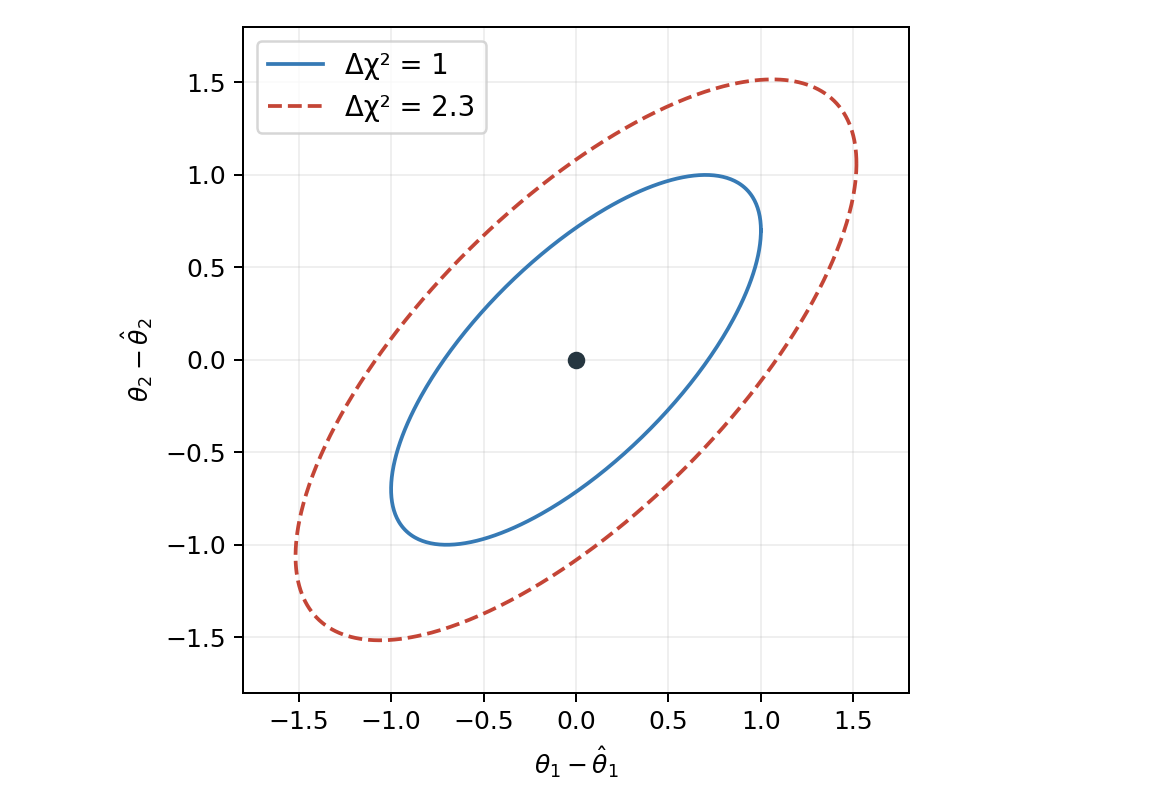
\includegraphics[keepaspectratio]{chapters/../assets/figures/lsq_quadratic_chi2_surface.png}}

}

\caption{\label{fig-least-squares-quadratic-surface}Контуры квадратичной
формы для двух параметров с единичными стандартными ошибками и
корреляцией \(\rho=0.7\). Сплошной контур соответствует \(c=1\),
пунктирный --- \(c=2.30\). Отложены отклонения параметров от минимума.}

\end{figure}%

Порог для совместной области зависит от числа параметров. Для двух
гауссовых оценок область с \(c=1\) покрывает истинную пару всего
примерно в \(39.3\%\) опытов. Для покрытия \(68.3\%\) требуется
\(c\simeq2.30\). Это тот же результат, который мы получили для
двумерного гаусса. Число измерений \(N\) здесь не заменяет число
параметров \(p\).

\subsection{Когда эллипса
недостаточно}\label{ux43aux43eux433ux434ux430-ux44dux43bux43bux438ux43fux441ux430-ux43dux435ux434ux43eux441ux442ux430ux442ux43eux447ux43dux43e}

В осцилляционной задаче разные частоты могут давать близкие предсказания
в точках измерения. Для иллюстрации возьмём четыре безразмерных момента
\(t_i=i\), \(i=1,\ldots,4\), и значения \(y_i=0.6\sin(1.2t_i)\). Это
специально заданные точки без добавленной случайной флуктуации. Приписав
им независимые гауссовы ошибки \(s=0.15\), получим функцию

\begin{equation}\protect\phantomsection\label{eq-ch12-oscillatory-example}{
\chi^2(A,\omega)=\sum_{i=1}^4
\frac{[y_i-A\sin(\omega t_i)]^2}{s^2}.
}\end{equation}

На рисунке \ref{fig-least-squares-nongaussian-surface} видны две
разделённые области. У этой учебной модели есть точная неоднозначность:
при целых \(t_i\) частоты \(\omega\) и \(\omega+2\pi\) дают те же
значения синуса.

\begin{figure}[H]

\centering{

\pandocbounded{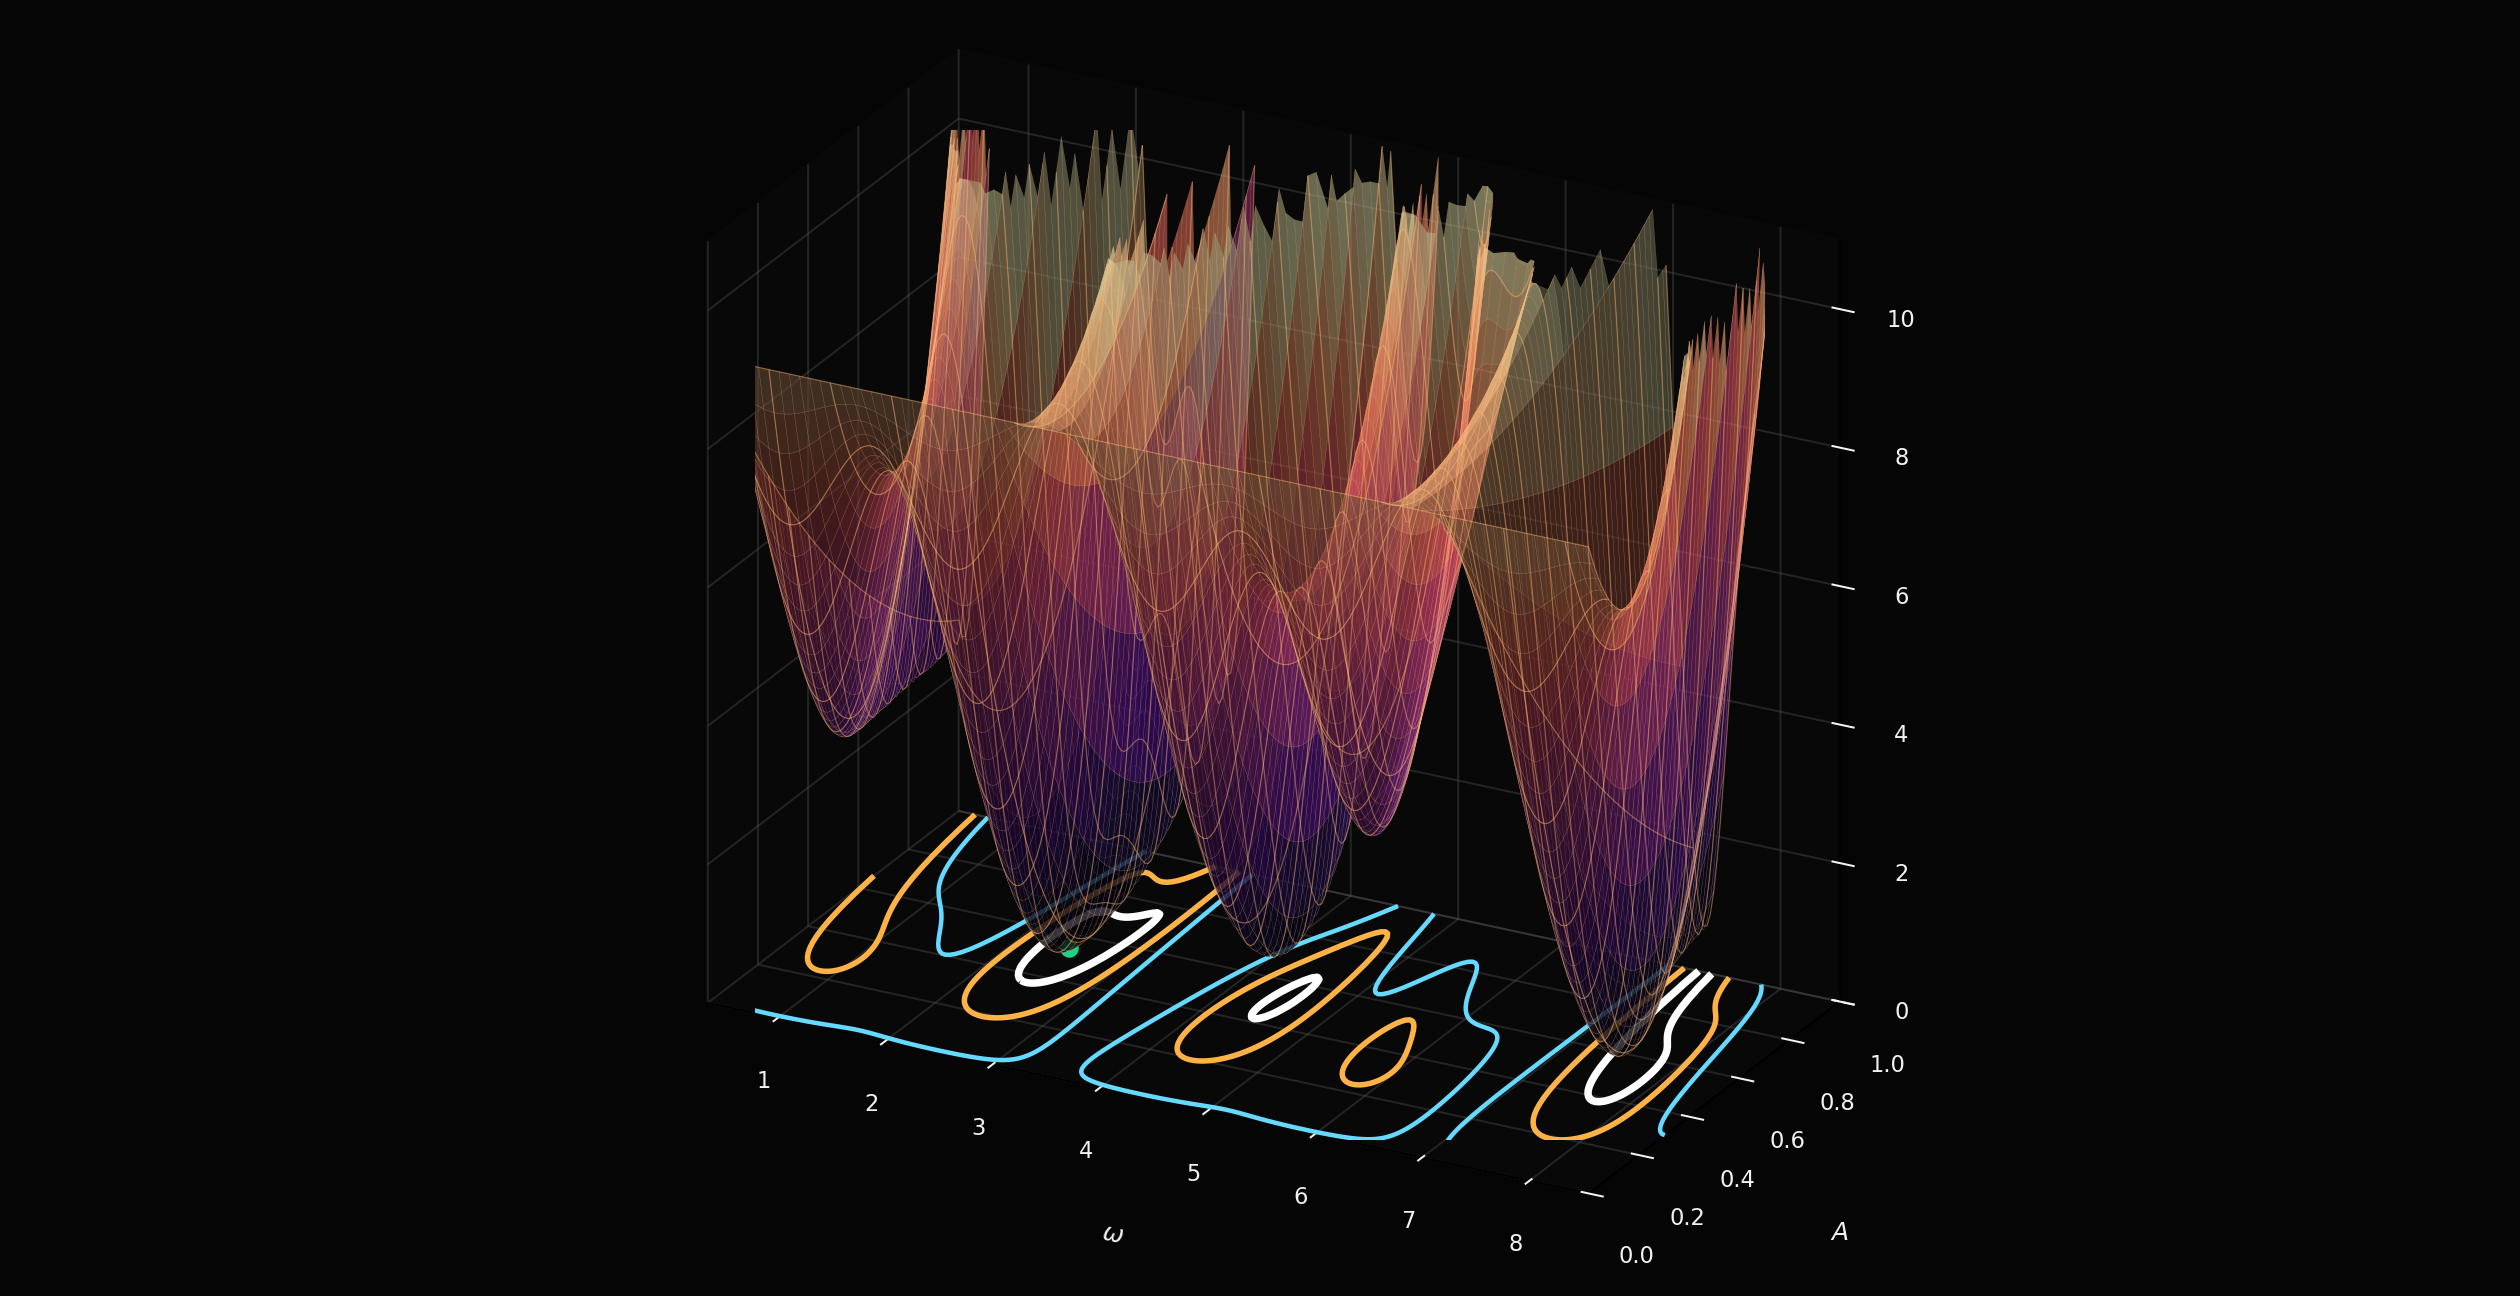
\includegraphics[keepaspectratio]{chapters/../assets/figures/lsq_oscillatory_chi2_surface.png}}

}

\caption{\label{fig-least-squares-nongaussian-surface}Контуры
\(\Delta\chi^2=1\), \(2.30\) и \(6.18\) для четырёх точек осцилляционной
модели. Минимумы при \(A=0.6\), \(\omega=1.2\) и \(\omega=1.2+2\pi\)
дают одинаковые предсказания. Локальный эллипс около одного минимума не
описывает вторую область.}

\end{figure}%

Можно очень точно вычислить вторые производные около первого минимума и
полностью пропустить второй. Поэтому в нелинейной задаче следует
исследовать весь допустимый диапазон параметров. Сами нарисованные
контуры ещё не имеют гарантированного доверительного уровня: его
проверяют по распределению статистики. Этим займёмся в следующей главе.

\section{Откуда берутся систематические
неопределённости}\label{ux43eux442ux43aux443ux434ux430-ux431ux435ux440ux443ux442ux441ux44f-ux441ux438ux441ux442ux435ux43cux430ux442ux438ux447ux435ux441ux43aux438ux435-ux43dux435ux43eux43fux440ux435ux434ux435ux43bux451ux43dux43dux43eux441ux442ux438}

Вернёмся к эксперименту. Сечение зависит от светимости и эффективности,
энергия --- от калибровки детектора, число сигнальных событий --- от
описания фона. Все эти величины входят в модель. Если они известны
неточно, их неопределённость передаётся результату.

Параметры, ради которых проводится измерение, называются
\textbf{параметрами интереса}. Остальные неизвестные параметры, влияющие
на предсказание, --- \textbf{мешающие параметры}. Например, в измерении
сечения светимость является мешающим параметром. В отдельной работе по
калибровке светимости она сама станет параметром интереса. Название
определяется задачей анализа.

Обозначим эти две группы через \(\boldsymbol\theta\) и
\(\boldsymbol\eta\):

\begin{equation}\protect\phantomsection\label{eq-ch12-nuisance-model}{
\boldsymbol\lambda=\boldsymbol\lambda(\boldsymbol\theta,\boldsymbol\eta).
}\end{equation}

Систематикой в разговоре называют источник неопределённости: шкалу
энергии, нормировку потока, форму фона. Для расчёта нужно уточнить, как
именно этот источник меняет \(\boldsymbol\lambda\) и какими данными
ограничены его параметры. Одного числа «систематическая ошибка \(5\%\)»
для произвольной подгонки мало.

\subsection{Вспомогательное измерение и
штраф}\label{ux432ux441ux43fux43eux43cux43eux433ux430ux442ux435ux43bux44cux43dux43eux435-ux438ux437ux43cux435ux440ux435ux43dux438ux435-ux438-ux448ux442ux440ux430ux444}

Пусть независимая калибровка дала вектор \(\mathbf z\). В гауссовом
приближении её вероятностная модель имеет вид

\begin{equation}\protect\phantomsection\label{eq-ch12-auxiliary-likelihood}{
\mathbf Z\sim\mathcal N(\boldsymbol\eta,V_\eta),
\qquad
L(\boldsymbol\theta,\boldsymbol\eta)
=L_{\mathrm{main}}(\mathbf y\mid\boldsymbol\theta,\boldsymbol\eta)
L_{\mathrm{aux}}(\mathbf z\mid\boldsymbol\eta).
}\end{equation}

Матрица \(V_\eta\) здесь описывает разброс \textbf{результата
калибровки} \(\mathbf Z\) при фиксированном \(\boldsymbol\eta\). В
частотной постановке сам неизвестный параметр не становится случайным.
Запись «\(\eta=\eta_0\pm s_\eta\)» означает результат вспомогательного
измерения; его полученное значение \(\eta_0\) играет роль \(z\).

При известных постоянных ковариациях и независимости двух наборов данных
произведение правдоподобий даёт сумму

\begin{equation}\protect\phantomsection\label{eq-ch12-constrained-chi-square}{
\begin{aligned}
\chi^2(\boldsymbol\theta,\boldsymbol\eta)
={}&[\mathbf y-\boldsymbol\lambda(\boldsymbol\theta,\boldsymbol\eta)]^{\mathsf T}
V_y^{-1}[\mathbf y-\boldsymbol\lambda(\boldsymbol\theta,\boldsymbol\eta)]\\
&+(\boldsymbol\eta-\mathbf z)^{\mathsf T}
V_\eta^{-1}(\boldsymbol\eta-\mathbf z).
\end{aligned}
}\end{equation}

Второе слагаемое называют \textbf{штрафным членом}. Сдвиг одного
калибровочного параметра на его стандартную ошибку добавляет единицу к
\(\chi^2\), если других коррелированных калибровочных параметров нет.
Основные данные могут предпочесть такой сдвиг. Совместная подгонка
сравнит улучшение описания основных данных с ухудшением описания
калибровки.

Если внешней информации нет, соответствующий штраф отсутствует: параметр
определяется только основными данными. Данных может оказаться
недостаточно, например для разделения общей нормировки и самого сечения.
Если калибровка использует те же события, что и основной анализ,
перемножать правдоподобия как независимые нельзя --- общие данные будут
учтены дважды.

Не всякая систематика получена из гауссовой калибровки. Интервал между
двумя теоретическими моделями сам по себе не задаёт ни гауссову ошибку,
ни стандартное отклонение. Для такого ограничения требуется отдельное
обоснование; формула \ref{eq-ch12-constrained-chi-square} его не
создаёт.

\section{Профилирование мешающих
параметров}\label{ux43fux440ux43eux444ux438ux43bux438ux440ux43eux432ux430ux43dux438ux435-ux43cux435ux448ux430ux44eux449ux438ux445-ux43fux430ux440ux430ux43cux435ux442ux440ux43eux432}

При каждом фиксированном \(\boldsymbol\theta\) найдём минимум по
\(\boldsymbol\eta\):

\begin{equation}\protect\phantomsection\label{eq-ch12-profile-definition}{
\chi^2_{\mathrm p}(\boldsymbol\theta)
=\min_{\boldsymbol\eta}\chi^2(\boldsymbol\theta,\boldsymbol\eta)
=\chi^2\!\left(\boldsymbol\theta,
\widehat{\widehat{\boldsymbol\eta}}(\boldsymbol\theta)\right).
}\end{equation}

Двойная шляпка обозначает результат этой условной подгонки. При
изменении параметра интереса калибровочные параметры могут сдвигаться,
частично компенсируя изменение предсказания. Поэтому профиль обычно шире
сечения, в котором все \(\boldsymbol\eta\) удерживаются в точке общего
минимума.

В квадратичном приближении тот же эффект виден из матрицы \(K\).
Разобьём её на блоки по двум группам параметров:

\begin{equation}\protect\phantomsection\label{eq-ch12-profile-curvature}{
K=\begin{pmatrix}
K_{\theta\theta}&K_{\theta\eta}\\
K_{\eta\theta}&K_{\eta\eta}
\end{pmatrix},
\qquad
K_{\mathrm p}=K_{\theta\theta}
-K_{\theta\eta}K_{\eta\eta}^{-1}K_{\eta\theta}.
}\end{equation}

Подстановка минимума по \(\boldsymbol\eta\) даёт кривизну профиля
\(K_{\mathrm p}\). Обратная матрица \(K_{\mathrm p}^{-1}\) совпадает с
\(\theta\theta\)-блоком полной матрицы \(K^{-1}\). Обратить только блок
\(K_{\theta\theta}\) --- значит получить ошибку при фиксированных
мешающих параметрах. Это другой расчёт.

\subsection{Линейная зависимость от
систематики}\label{ux43bux438ux43dux435ux439ux43dux430ux44f-ux437ux430ux432ux438ux441ux438ux43cux43eux441ux442ux44c-ux43eux442-ux441ux438ux441ux442ux435ux43cux430ux442ux438ux43aux438}

Часть минимизации можно выполнить аналитически. При фиксированном
\(\boldsymbol\theta\) разложим предсказание около результата калибровки
\(\mathbf z\):

\begin{equation}\protect\phantomsection\label{eq-ch12-linear-systematics}{
\begin{aligned}
\boldsymbol\lambda(\boldsymbol\theta,\boldsymbol\eta)
&\simeq\boldsymbol\lambda_0(\boldsymbol\theta)+H(\boldsymbol\theta)\boldsymbol\delta,\\
\boldsymbol\delta&=\boldsymbol\eta-\mathbf z,
\qquad
H_{ij}=\left.\frac{\partial\lambda_i}{\partial\eta_j}\right|_{\boldsymbol\eta=\mathbf z}.
\end{aligned}
}\end{equation}

Здесь
\(\boldsymbol\lambda_0=\boldsymbol\lambda(\boldsymbol\theta,\mathbf z)\),
а \(H\) содержит \(N\) строк и столько столбцов, сколько имеется
мешающих параметров. Каждый столбец показывает согласованное изменение
всех предсказаний при сдвиге одного параметра.

\begin{bookderivation}

\subsection{Аналитический
минимум}\label{ux430ux43dux430ux43bux438ux442ux438ux447ux435ux441ux43aux438ux439-ux43cux438ux43dux438ux43cux443ux43c}

Положим \(W=V_y^{-1}\), \(C=V_\eta\) и
\(\mathbf r=\mathbf y-\boldsymbol\lambda_0\). Тогда

\begin{equation}\protect\phantomsection\label{eq-ch12-linear-penalty}{
\chi^2=(\mathbf r-H\boldsymbol\delta)^{\mathsf T}
W(\mathbf r-H\boldsymbol\delta)
+\boldsymbol\delta^{\mathsf T}C^{-1}\boldsymbol\delta.
}\end{equation}

Производная по \(\boldsymbol\delta\) даёт систему

\begin{equation}\protect\phantomsection\label{eq-ch12-nuisance-normal-equations}{
(C^{-1}+H^{\mathsf T}WH)\widehat{\widehat{\boldsymbol\delta}}
=H^{\mathsf T}W\mathbf r.
}\end{equation}

Обозначим матрицу слева через \(M\). В минимуме
\(\widehat{\widehat{\boldsymbol\delta}}=M^{-1}H^{\mathsf T}W\mathbf r\).
Подставим это решение в исходную сумму квадратов:

\begin{equation}\protect\phantomsection\label{eq-ch12-profile-after-substitution}{
\chi^2_{\mathrm p}
=\mathbf r^{\mathsf T}
\left(W-WHM^{-1}H^{\mathsf T}W\right)\mathbf r.
}\end{equation}

Матрицу в скобках можно записать как \((V_y+HCH^{\mathsf T})^{-1}\).
Равенство проверяется умножением на \(V_y+HCH^{\mathsf T}\). Получаем

\begin{equation}\protect\phantomsection\label{eq-ch12-effective-covariance}{
\chi^2_{\mathrm p}(\boldsymbol\theta)
=\mathbf r^{\mathsf T}V^{-1}\mathbf r,
\qquad
V=V_y+HV_\eta H^{\mathsf T}.
}\end{equation}

\end{bookderivation}

Второе слагаемое в \(V\) знакомо по распространению ошибок. Если одна
калибровка влияет на много точек, её вклад обычно недиагонален. Добавить
соответствующие дисперсии только к диагонали --- значит потерять эту
связь.

Для точно линейной зависимости от \(\boldsymbol\eta\) и гауссова штрафа
формула \ref{eq-ch12-effective-covariance} точна при каждом
фиксированном \(\boldsymbol\theta\). Если использовано лишь линейное
разложение, нужно проверить его во всём диапазоне сдвигов, допускаемых
подгонкой.

\subsection{\texorpdfstring{Нужно ли теперь добавлять
\(\ln\det V\)?}{Нужно ли теперь добавлять \textbackslash ln\textbackslash det V?}}\label{ux43dux443ux436ux43dux43e-ux43bux438-ux442ux435ux43fux435ux440ux44c-ux434ux43eux431ux430ux432ux43bux44fux442ux44c-lndet-v}

Нет. В формуле \ref{eq-ch12-effective-covariance} мы уже выполнили
минимизацию исходного \(\chi^2\). Его нормировочные множители
определялись постоянными \(V_y\) и \(V_\eta\). Определитель эффективной
матрицы после минимизации не появился, даже если \(H\) зависит от
\(\boldsymbol\theta\).

У формулы \ref{eq-ch12-gaussian-variable-covariance} другая исходная
постановка: там зависимость ковариации от параметров задана в самой
плотности данных. Интегрирование гауссова выражения по мешающим
параметрам также создаёт зависящий от ширины множитель. Профилирование
такого интегрирования не выполняет. Чтобы выбрать нужное выражение,
следует вернуться к исходному правдоподобию.

\section{Возвращаемся к общей
нормировке}\label{ux432ux43eux437ux432ux440ux430ux449ux430ux435ux43cux441ux44f-ux43a-ux43eux431ux449ux435ux439-ux43dux43eux440ux43cux438ux440ux43eux432ux43aux435}

Запишем модель для данных \ref{eq-ch12-normalization-data}:

\begin{equation}\protect\phantomsection\label{eq-ch12-normalization-measurement-model}{
Y_i=(1+\alpha)\mu+\varepsilon_i,
\qquad
\varepsilon_i\sim\mathcal N(0,s_i^2),
\qquad
Z\sim\mathcal N(\alpha,f_N^2).
}\end{equation}

Все \(\varepsilon_i\) и результат калибровки \(Z\) независимы.
Полученное значение калибровки равно \(z=0\), то есть номинальный
масштаб равен единице. Параметр \(\alpha\) безразмерный и один для обеих
точек. Линейная запись масштаба соответствует нашей модели относительной
неопределённости; интересующая область находится далеко от нефизического
значения \(1+\alpha\le0\).

Полная функция для подгонки равна

\begin{equation}\protect\phantomsection\label{eq-ch12-normalization-penalty}{
\chi^2(\mu,\alpha)
=\sum_i\frac{[y_i-(1+\alpha)\mu]^2}{s_i^2}
+\frac{\alpha^2}{f_N^2}.
}\end{equation}

Введём статистически взвешенное среднее \(m\), его дисперсию \(v\) при
фиксированной нормировке и сумму квадратов отклонений от этого среднего:

\begin{equation}\protect\phantomsection\label{eq-ch12-normalization-statistical-sums}{
S=\sum_i\frac1{s_i^2},\qquad
m=\frac1S\sum_i\frac{y_i}{s_i^2},\qquad
v=\frac1S,\qquad
q_0=\sum_i\frac{(y_i-m)^2}{s_i^2}.
}\end{equation}

Поскольку \(\sum_i(y_i-m)/s_i^2=0\), функция распадается на три
слагаемых:

\begin{equation}\protect\phantomsection\label{eq-ch12-normalization-decomposition}{
\chi^2(\mu,\alpha)
=q_0+\frac{[m-(1+\alpha)\mu]^2}{v}
+\frac{\alpha^2}{f_N^2}.
}\end{equation}

Последние два слагаемых неотрицательны и одновременно обращаются в нуль
при \(\widehat\alpha=0\), \(\widehat\mu=m\). Это и есть общий минимум.
Две точки определяют произведение \((1+\alpha)\mu\), а разделить его на
масштаб и сечение позволяет вспомогательная калибровка.

\subsection{Профиль и ошибка
сечения}\label{ux43fux440ux43eux444ux438ux43bux44c-ux438-ux43eux448ux438ux431ux43aux430-ux441ux435ux447ux435ux43dux438ux44f}

При фиксированном \(\mu\) минимум по \(\alpha\) имеет вид

\begin{equation}\protect\phantomsection\label{eq-ch12-normalization-profile}{
\widehat{\widehat\alpha}(\mu)
=\frac{f_N^2\mu(m-\mu)}{v+f_N^2\mu^2},
\qquad
\chi^2_{\mathrm p}(\mu)
=q_0+\frac{(m-\mu)^2}{v+f_N^2\mu^2}.
}\end{equation}

Профиль уже не парабола: его знаменатель зависит от \(\mu\). Вблизи
минимума достаточно подставить в знаменатель \(\mu=m\). Отсюда локальная
ошибка

\begin{equation}\protect\phantomsection\label{eq-ch12-normalization-local-error}{
\sigma_\mu^2\simeq v+f_N^2m^2.
}\end{equation}

Первое слагаемое уменьшается при накоплении статистики. Второе остаётся,
пока точность общей калибровки прежняя. Два набора событий не превращают
одну калибровку в две независимые.

Для наших чисел получаем

\begin{equation}\protect\phantomsection\label{eq-ch12-normalization-numbers}{
m=8.23486\ \text{пб},\qquad
v=0.013575\ \text{пб}^2,\qquad
f_N^2m^2=0.678130\ \text{пб}^2.
}\end{equation}

Это объясняет результат \ref{eq-ch12-normalization-first-result}. Полная
локальная ковариация по \((\mu,\alpha)\) равна

\begin{equation}\protect\phantomsection\label{eq-ch12-normalization-joint-covariance}{
V_{\mu,\alpha}\simeq
\begin{pmatrix}
v+f_N^2m^2&-f_N^2m\\
-f_N^2m&f_N^2
\end{pmatrix}.
}\end{equation}

Верхний левый элемент имеет размерность пб\(^2\), внедиагональный ---
пб, нижний правый безразмерный. Отрицательная ковариация соответствует
модели: увеличение масштаба компенсируется уменьшением сечения.

Для границ по \(\Delta\chi^2_{\mathrm p}=1\) можно использовать весь
профиль \ref{eq-ch12-normalization-profile}. При \(f_N<1\) решение имеет
вид

\begin{equation}\protect\phantomsection\label{eq-ch12-normalization-profile-limits}{
\mu_\pm=
\frac{m\pm\sqrt{f_N^2m^2+(1-f_N^2)v}}{1-f_N^2}.
}\end{equation}

Интервал получится асимметричным. Формула для границ точна для заданной
функции, но её покрытие в нелинейной модели требует отдельной проверки.
Симметричная ошибка \(0.832\) пб описывает только местную кривизну.

\subsection{Та же задача через
ковариацию}\label{ux442ux430-ux436ux435-ux437ux430ux434ux430ux447ux430-ux447ux435ux440ux435ux437-ux43aux43eux432ux430ux440ux438ux430ux446ux438ux44e}

Производная предсказания по \(\alpha\) равна \(\mu\) для каждой точки.
По формуле \ref{eq-ch12-effective-covariance}

\begin{equation}\protect\phantomsection\label{eq-ch12-model-normalization-covariance}{
V_{ij}(\mu)=s_i^2\delta_{ij}+f_N^2\mu^2.
}\end{equation}

Весь нормировочный вклад пропорционален матрице из единиц. Подстановка
этой матрицы в \(\mathbf r^{\mathsf T}V(\mu)^{-1}\mathbf r\) даёт ровно
профиль \ref{eq-ch12-normalization-profile}. Таким способом можно
выполнить ту же подгонку без явного параметра \(\alpha\).

Если зафиксировать \(V\) при \(\mu=m\), получится парабола с тем же
минимумом и той же кривизной. Вдали от минимума она отличается от
точного профиля. Эквивалентность центрального значения и локальной
ошибки не означает совпадения всей функции.

\section{Парадокс
Д'Агостини}\label{ux43fux430ux440ux430ux434ux43eux43aux441-ux434ux430ux433ux43eux441ux442ux438ux43dux438}

Теперь построим нормировочную матрицу из измеренных значений, заменив
\(\mu^2\) на \(y_i y_j\):

\begin{equation}\protect\phantomsection\label{eq-ch12-data-normalization-covariance}{
\begin{aligned}
V_{\mathrm{data}}
&=\begin{pmatrix}s_1^2&0\\0&s_2^2\end{pmatrix}
+f_N^2\begin{pmatrix}y_1^2&y_1y_2\\y_1y_2&y_2^2\end{pmatrix}\\
&=\begin{pmatrix}0.6656&0.6800\\0.6800&0.7514\end{pmatrix}\ \text{пб}^2.
\end{aligned}
}\end{equation}

С этой фиксированной матрицей минимизируем
\((\mathbf y-\mu\mathbf1)^{\mathsf T}V_{\mathrm{data}}^{-1}
(\mathbf y-\mu\mathbf1)\), где \(\mathbf1\) --- вектор из единиц.
Решение для произвольной известной фиксированной матрицы \(V\) равно

\begin{equation}\protect\phantomsection\label{eq-ch12-correlated-mean-weights}{
\widehat\mu=\mathbf w^{\mathsf T}\mathbf y,
\qquad
\mathbf w=\frac{V^{-1}\mathbf1}{\mathbf1^{\mathsf T}V^{-1}\mathbf1},
\qquad
\sigma_\mu^2=\frac1{\mathbf1^{\mathsf T}V^{-1}\mathbf1}.
}\end{equation}

При \(V=V_{\mathrm{data}}\) веса составляют примерно \(w_1=1.253\),
\(w_2=-0.253\). Отсюда и получается \(7.87\pm0.81\) пб. Ошибка после
знака \(\pm\) здесь формально вычислена по кривизне: матрица построена
из тех же случайных данных, поэтому считать её результат истинным
стандартным отклонением оценки без проверки нельзя.

Отрицательные веса сами по себе допустимы при объединении
коррелированных измерений. Их сумма равна единице, но каждый вес не
обязан лежать между нулём и единицей. В нашей задаче ошибка состоит в
конкретной подстановке \(f_N^2y_i y_j\): направление изменения всех
предсказаний задаётся общим сечением \(\mu\), а здесь оно стало зависеть
от отдельных флуктуаций точек.

\subsection{Как появляется
сдвиг}\label{ux43aux430ux43a-ux43fux43eux44fux432ux43bux44fux435ux442ux441ux44f-ux441ux434ux432ux438ux433}

Для двух точек обращение матрицы
\ref{eq-ch12-data-normalization-covariance} даёт простой ответ:

\begin{equation}\protect\phantomsection\label{eq-ch12-dagostini-shift}{
\widehat\mu_{\mathrm{data}}
=\frac{m}{1+f_N^2q_0},
\qquad
q_0=\frac{(y_1-y_2)^2}{s_1^2+s_2^2}.
}\end{equation}

Чем сильнее расходятся точки, тем больше знаменатель. Для положительного
\(m\) такая конструкция уменьшает центральное значение. В нашем примере
\(q_0\simeq4.59\), и множитель \(1/(1+f_N^2q_0)\) равен примерно
\(0.956\). Минимизация воспроизводит то, что ей было задано формулой.

Пример разбирается в работе Д'Агостини {[}1{]}. Он показывает, почему
правила распространения ошибок нельзя переносить в подгонку без проверки
зависимости ковариации от данных и параметров.

\subsection{Интерактив: меняем общую
ошибку}\label{interactive-least-squares-normalization}

Меняйте \(f_N\), оставляя обе точки и их независимые ошибки прежними. На
верхнем графике сравниваются центральные значения, полученные двумя
способами. На нижнем показаны точный профиль модели с общей нормировкой
и квадратичная функция с матрицей из данных. Из каждой функции вычтен её
собственный минимум.

\begin{semanticpdfbox}[breakable=false]

\begin{center}

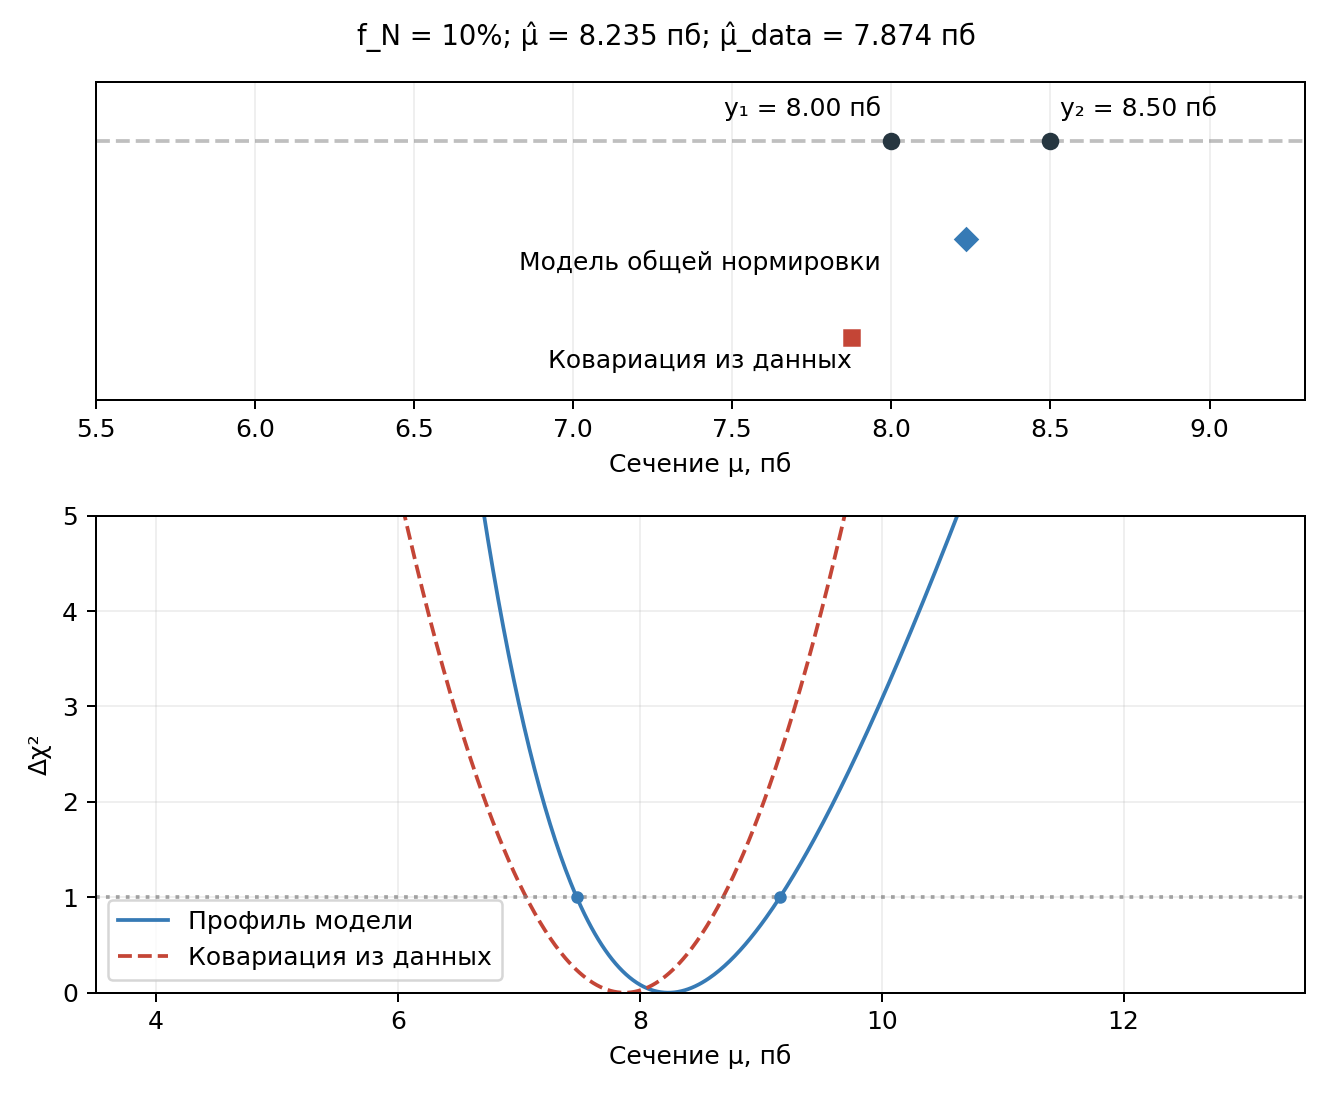
\includegraphics[width=0.74\linewidth,height=\textheight,keepaspectratio,alt={Общая нормировка: модель и подстановка данных}]{assets/figures/lsq_dagostini_comparison.png}

\end{center}

\noindent\begin{minipage}[c]{\dimexpr\linewidth-30mm\relax}

\textbf{Интерактив}. \textbf{Общая нормировка: модель и подстановка
данных}

При \(f_N=0.10\) модель даёт центральное значение \(8.235\) пб, а
подстановка данных в нормировочную ковариацию --- \(7.874\) пб. Профиль
модели асимметричен; пунктирная функция с фиксированной матрицей
является параболой.

\end{minipage}\hfill\begin{minipage}[c]{26mm}\centering

\href{https://neutrinohit.github.io/statistical-analysis-course/ru/book/chapters/12_least_squares_systematics.html\#interactive-least-squares-normalization}{
\includegraphics[width=24mm,height=\textheight,keepaspectratio,alt={QR-код интерактива}]{assets/qr/least-squares-normalization.png}}

\end{minipage}

\end{semanticpdfbox}

При \(f_N=0\) обе процедуры совпадают. С ростом \(f_N\) профиль
расширяется, но его минимум остаётся при \(m\). Минимум функции с
\(V_{\mathrm{data}}\) уходит в сторону меньших значений.

\section{Распространение ошибок после
подгонки}\label{ux440ux430ux441ux43fux440ux43eux441ux442ux440ux430ux43dux435ux43dux438ux435-ux43eux448ux438ux431ux43eux43a-ux43fux43eux441ux43bux435-ux43fux43eux434ux433ux43eux43dux43aux438}

Подогнанные параметры часто нужны для вычисления другой величины
\(\mathbf g(\boldsymbol\theta)\). Закон распространения ошибок остаётся
тем же, что и в главе 6:

\begin{equation}\protect\phantomsection\label{eq-ch12-post-fit-propagation}{
\widehat{\mathbf g}=\mathbf g(\widehat{\boldsymbol\theta}),
\qquad
V_g\simeq J V_\theta J^{\mathsf T},
\qquad
J_{ij}=\left.\frac{\partial g_i}{\partial\theta_j}\right|_{\widehat{\boldsymbol\theta}}.
}\end{equation}

Матрица \(V_\theta\) должна включать влияние подогнанных мешающих
параметров. Если сама \(\mathbf g\) зависит ещё и от
\(\boldsymbol\eta\), в якобиан и ковариацию включается полный набор
\((\boldsymbol\theta,\boldsymbol\eta)\). Уже учтённую при подгонке
систематику второй раз в квадратуру не добавляют.

Например, после калибровки \(y=a+bx\) энергия нового сигнала \(y_*\)
оценивается как \(\widehat E=(y_*-\widehat a)/\widehat b\). Если
измерение \(y_*\) независимо от калибровки и имеет дисперсию \(s_*^2\),
то в линейном приближении

\begin{equation}\protect\phantomsection\label{eq-ch12-inverse-calibration-error}{
\operatorname{Var}(\widehat E)\simeq
\frac{s_*^2+\operatorname{Var}(\widehat a)
+\widehat E^2\operatorname{Var}(\widehat b)
+2\widehat E\operatorname{cov}(\widehat a,\widehat b)}{\widehat b^2}.
}\end{equation}

Ковариационный член может существенно уменьшить ошибку, как и для прямой
калибровки в прошлой главе. Если \(\widehat b\) близко к нулю или его
ошибка велика, отношение уже нельзя надёжно описывать этим линейным
разложением.

\section{Что проверить перед записью
результата}\label{ux447ux442ux43e-ux43fux440ux43eux432ux435ux440ux438ux442ux44c-ux43fux435ux440ux435ux434-ux437ux430ux43fux438ux441ux44cux44e-ux440ux435ux437ux443ux43bux44cux442ux430ux442ux430}

Найденный минимум и его кривизна относятся к той модели, которую мы
записали. Если исходные данные --- малые пуассоновские счёты, гауссову
сумму квадратов нужно заменить соответствующим правдоподобием. Если
заметны ошибки по \(x\), модель должна описывать обе измеренные
координаты. Например, истинные координаты точек можно ввести как
дополнительные мешающие параметры. Одного увеличения вертикальных ошибок
для произвольной кривой недостаточно.

При нелинейной подгонке полезно сравнить профиль с параболой, проверить
границы допустимых параметров и несколько начальных точек минимизации.
Кривизна в одном минимуме не сообщает о других решениях.

В публикации вместе со значениями и единицами параметров нужны их
ковариации, использованная функция подгонки и описание внешних
ограничений. По этим сведениям другой исследователь сможет повторить
расчёт или объединить результат со своим. Для нашей пары чисел особенно
существенно, что ошибка нормировки общая: два независимых вклада по
\(10\%\) дали бы другую задачу.

Остаётся ещё вопрос: насколько полученное \(\chi^2_{\min}\) типично для
верной модели? Здесь требуется распределение минимума в ансамбле
экспериментов. Оно отличается от распределения приращения
\(\Delta\chi^2\), используемого для интервалов. Разберём это в следующей
главе.

\begin{bookchaptersummary}[Итоги главы]

\begin{itemize}
\tightlist
\item
  Коррелированные измерения входят в МНК через полную ковариацию.
  Локальная обратная ковариация параметров равна половине матрицы вторых
  производных \(\chi^2\) в минимуме.
\item
  Интервалы одного параметра строят по профилю, а совместные области
  требуют порога для соответствующего числа параметров. Вне линейной
  гауссовой задачи покрытие нужно обосновывать отдельно.
\item
  Независимая гауссова калибровка даёт штрафной член. Линейное влияние
  мешающих параметров позволяет выполнить профилирование аналитически и
  получить эффективную ковариацию \(V_y+HV_\eta H^{\mathsf T}\).
\item
  Общая нормировка меняет все предсказания согласованно. Подстановка
  отдельных измеренных значений вместо модельного масштаба может
  сместить результат; уже учтённую систематику не добавляют повторно
  после подгонки.
\end{itemize}

\end{bookchaptersummary}

\section{Задачи}\label{ux437ux430ux434ux430ux447ux438-11}

\begin{semanticpdfbox}[colback=BookCoralSoft,borderline west={1.2mm}{0pt}{BookCoral},breakable=false]

\noindent{\sffamily\bfseries\fontsize{11.2}{13.5}\selectfont Задача 1. Коррелированные измерения}\par\nopagebreak[4]\vspace{1.2mm}

Три гауссовых измерения \(Y_i\) имеют общее среднее \(\mu\) и известную
ковариацию \[
V=\sigma^2
\begin{pmatrix}
1&\rho&\rho\\
\rho&1&\rho\\
\rho&\rho&1
\end{pmatrix},
\qquad \sigma>0,\quad -\tfrac12<\rho<1.
\]

\begin{enumerate}
\def\labelenumi{\arabic{enumi}.}
\tightlist
\item
  Запишите \(\chi^2(\mu)\), найдите оценку \(\widehat\mu\) и её
  дисперсию.
\item
  Объясните, почему \(\rho\) меняет ошибку, но не меняет центральное
  значение.
\item
  Исследуйте пределы \(\rho\to0\), \(\rho\to1\) и \(\rho\to-1/2\)
  изнутри допустимого интервала. Что происходит с собственными
  значениями \(V\) на границах?
\item
  Сравните истинную дисперсию оценки с ошибкой, которую вы сообщили бы
  при игнорировании корреляций.
\end{enumerate}

\end{semanticpdfbox}

\begin{semanticpdfbox}[colback=BookCoralSoft,borderline west={1.2mm}{0pt}{BookCoral},breakable=false]

\noindent{\sffamily\bfseries\fontsize{11.2}{13.5}\selectfont Задача 2. Одна калибровка для многих измерений}\par\nopagebreak[4]\vspace{1.2mm}

Результаты описываются моделью \(Y_i=\mu+\eta+\varepsilon_i\),
\(i=1,\ldots,N\), где \(\varepsilon_i\) независимы и имеют распределение
\(\mathcal N(0,s^2)\). Независимая калибровка даёт
\(Z\sim\mathcal N(\eta,\tau^2)\). Параметры \(\mu,\eta\) фиксированы,
дисперсии \(s^2,\tau^2>0\) известны.

\begin{enumerate}
\def\labelenumi{\arabic{enumi}.}
\tightlist
\item
  Запишите совместный \(\chi^2(\mu,\eta)\) для полученных \(y_i\) и
  \(z\).
\item
  Найдите общий минимум, профиль по \(\mu\) и дисперсию оценки
  \(\widehat\mu\).
\item
  Проверьте эквивалентную запись с остатками \(y_i-z-\mu\) и матрицей
  \(V=s^2I+\tau^2\mathbf1\mathbf1^{\mathsf T}\), где \(I\) --- единичная
  матрица, \(\mathbf1\) --- вектор из единиц.
\item
  Что происходит с ошибкой \(\widehat\mu\) при \(N\to\infty\)? Что
  получилось бы, если ошибочно добавить \(\tau^2\) только к диагонали?
\item
  При \(\mu=10\), \(\eta=0.5\), \(s=1\), \(\tau=0.3\), \(N=20\)
  проверьте ответ псевдоэкспериментами. В каждом опыте заново
  генерируйте и основные данные, и калибровку.
\end{enumerate}

\end{semanticpdfbox}

\begin{semanticpdfbox}[colback=BookCoralSoft,borderline west={1.2mm}{0pt}{BookCoral},breakable=false]

\noindent{\sffamily\bfseries\fontsize{11.2}{13.5}\selectfont Задача 3. Кривизна и нелинейная подгонка}\par\nopagebreak[4]\vspace{1.2mm}

Средний сигнал имеет вид \(f(t)=A e^{-\lambda t}\). Сгенерируйте пять
независимых гауссовых измерений при \(t_i=0,1,2,3,4\) с, \(A=10\) мВ,
\(\lambda=0.5\) с\(^{-1}\) и известной одинаковой ошибке \(s=1\) мВ.
Зафиксируйте начальное состояние генератора.

\begin{enumerate}
\def\labelenumi{\arabic{enumi}.}
\tightlist
\item
  Подгоните \(A>0\) и \(\lambda\ge0\), используя несколько начальных
  точек.
\item
  В случае внутреннего минимума вычислите матрицу вторых производных
  \(\chi^2\) и локальную ковариацию. Проверьте множитель \(1/2\).
\item
  Постройте контур \(\Delta\chi^2=2.30\) и сравните с локальным
  эллипсом. Гарантирует ли само значение порога покрытие \(68.3\%\) в
  этой задаче?
\item
  Постройте профиль по \(\lambda\) и сечение с фиксированным
  \(\widehat A\).
\item
  Повторите расчёт при \(s=3\) мВ, сохранив те же стандартные гауссовы
  случайные числа. Исследуйте асимметрию профиля и влияние границы
  \(\lambda=0\).
\end{enumerate}

\end{semanticpdfbox}

\begin{semanticpdfbox}[colback=BookCoralSoft,borderline west={1.2mm}{0pt}{BookCoral},breakable=false]

\noindent{\sffamily\bfseries\fontsize{11.2}{13.5}\selectfont Задача 4. Общая нормировка}\par\nopagebreak[4]\vspace{1.2mm}

Даны \(y_1=8.00\) пб, \(y_2=8.50\) пб и известные независимые гауссовы
ошибки \(s_1=0.16\) пб, \(s_2=0.17\) пб. Модель имеет вид
\(Y_i=(1+\alpha)\mu+\varepsilon_i\). Независимая калибровка
\(Z\sim\mathcal N(\alpha,f_N^2)\) дала \(z=0\) при \(f_N=0.10\).

\begin{enumerate}
\def\labelenumi{\arabic{enumi}.}
\tightlist
\item
  Запишите совместный \(\chi^2\), найдите минимум и аналитический
  профиль по \(\mu\).
\item
  Вычислите локальную ковариацию \((\widehat\mu,\widehat\alpha)\) и
  границы \(\Delta\chi^2_{\mathrm p}=1\). Сравните их с
  \(\widehat\mu\pm\sigma_\mu\).
\item
  Постройте матрицу \(V_{ij}(\mu)=s_i^2\delta_{ij}+f_N^2\mu^2\) и
  численно проверьте эквивалентность профильной записи при нескольких
  \(\mu\).
\item
  Повторите подгонку с фиксированной матрицей
  \(V_{ij}=s_i^2\delta_{ij}+f_N^2y_i y_j\). Найдите веса и объясните
  сдвиг оценки.
\item
  Почему добавление \(\ln\det V(\mu)\) меняет исходную профильную
  задачу?
\end{enumerate}

\end{semanticpdfbox}

\begin{semanticpdfbox}[colback=BookCoralSoft,borderline west={1.2mm}{0pt}{BookCoral},breakable=false]

\noindent{\sffamily\bfseries\fontsize{11.2}{13.5}\selectfont Задача 5. Энергия по калибровке}\par\nopagebreak[4]\vspace{1.2mm}

Калибровка описывается прямой \(y=a+bE\). Получены \(\widehat a=2\)
канала, \(\widehat b=100\) каналов/МэВ,
\(\operatorname{Var}(\widehat a)=28/3\) канал\(^2\),
\(\operatorname{Var}(\widehat b)=2\) канал\(^2\)/МэВ\(^2\) и
\(\operatorname{cov}(\widehat a,\widehat b)=-4\) канал\(^2\)/МэВ. Новое
независимое измерение дало \(y_*=202\) канала с ошибкой \(s_*=2\)
канала.

\begin{enumerate}
\def\labelenumi{\arabic{enumi}.}
\tightlist
\item
  Найдите \(\widehat E=(y_*-\widehat a)/\widehat b\).
\item
  Выведите её дисперсию в линейном приближении и вычислите ошибку в МэВ.
\item
  Повторите расчёт, отбросив ковариацию. Насколько изменился ответ?
\item
  Ковариация калибровки уже включает общую систематическую
  неопределённость. Нужно ли добавлять её вклад к ошибке энергии ещё
  раз?
\item
  При каких значениях \(\widehat b\) и его ошибки линейное приближение
  для отношения требует проверки?
\end{enumerate}

\end{semanticpdfbox}

\section*{Литература}\label{ux43bux438ux442ux435ux440ux430ux442ux443ux440ux430-11}
\addcontentsline{toc}{section}{Литература}

\markright{Литература}

\protect\phantomsection\label{refs}
\begin{CSLReferences}{0}{0}
\bibitem[\citeproctext]{ref-dagostini1994bias}
{[}1{]} D'Agostini, G. On the Use of the Covariance Matrix to Fit
Correlated Data. \emph{Nuclear Instruments and Methods in Physics
Research Section A}, \textbf{346}, 306--311. 1994.
doi:\href{https://doi.org/10.1016/0168-9002(94)90719-6}{10.1016/0168-9002(94)90719-6}.

\bibitem[\citeproctext]{ref-cowan1998}
{[}2{]} Cowan, G. \emph{Statistical Data Analysis}. Oxford University
Press. 1998.

\end{CSLReferences}

\part{III. Статистический вывод}

\chapter{Качество согласия и статистическая
значимость}\label{ux43aux430ux447ux435ux441ux442ux432ux43e-ux441ux43eux433ux43bux430ux441ux438ux44f-ux438-ux441ux442ux430ux442ux438ux441ux442ux438ux447ux435ux441ux43aux430ux44f-ux437ux43dux430ux447ux438ux43cux43eux441ux442ux44c}

\bookchapteropeningcontents

\begin{bookchapteropening}[Аннотация]

Подгонка даёт параметры модели и их ошибки. В этой главе проверим,
насколько сама модель согласуется с данными. Выведем распределение χ²,
разберём число степеней свободы и научимся вычислять p-значение.
Вернёмся к графикам поиска бозона Хиггса из первой главы и выясним, что
означают линии «числа сигма». Для малых пуассоновских счётов получим
распределение статистики псевдоэкспериментами.

\end{bookchapteropening}

\section{Физическая задача: можно ли пользоваться
калибровкой?}\label{ux444ux438ux437ux438ux447ux435ux441ux43aux430ux44f-ux437ux430ux434ux430ux447ux430-ux43cux43eux436ux43dux43e-ux43bux438-ux43fux43eux43bux44cux437ux43eux432ux430ux442ux44cux441ux44f-ux43aux430ux43bux438ux431ux440ux43eux432ux43aux43eux439}

Мы откалибровали детектор по источникам с известными энергиями. В каждой
точке измерили среднюю амплитуду сигнала и подогнали прямую

\begin{equation}\protect\phantomsection\label{eq-ch13-calibration-model}{
y_i=a+bE_i+\varepsilon_i,
\qquad \varepsilon_i\sim\mathcal N(0,\sigma_i^2).
}\end{equation}

Здесь \(E_i\) --- энергия в МэВ, \(y_i\) --- амплитуда в каналах, \(a\)
--- смещение нуля, \(b\) --- коэффициент преобразования в каналах на
МэВ. Энергии считаем известными точно, ошибки амплитуд --- независимыми
и гауссовыми, а \(\sigma_i\) --- известными до подгонки.

Программа нашла \(\widehat a\), \(\widehat b\) и их ковариацию. Можно
теперь пересчитывать амплитуды в энергии? Только если прямая описывает
отклик детектора с нужной нам точностью. Электроника может давать
нелинейность; при больших амплитудах возможно насыщение. Минимизатор об
этом ничего не знает. Он найдёт наиболее подходящую прямую для тех
точек, которые ему передали.

Возьмём два учебных результата. В первой калибровке было \(N=12\) точек,
и после подгонки двух параметров получилось \(\chi^2_{\min}=12\). Во
второй --- \(N=1002\) точки и \(\chi^2_{\min}=1200\). Числа степеней
свободы равны соответственно \(10\) и \(1000\). В обоих случаях

\begin{equation}\protect\phantomsection\label{eq-ch13-same-reduced-chi-square}{
\frac{\chi^2_{\min}}{\nu}=1.2.
}\end{equation}

В физическом фольклоре отношение, близкое к единице, часто принимают за
достаточную проверку фита. Наши два примера показывают, чего в такой
проверке не хватает. При верной модели вероятность получить значение
\(\chi^2_{\min}\) не меньше указанного равна примерно \(0.285\) в первом
случае и \(1.23\cdot10^{-5}\) во втором.

Разница больше четырёх порядков. Давайте получим эти числа и разберёмся,
что именно они позволяют сказать о калибровке.

\section{Остатки и статистика качества
согласия}\label{ux43eux441ux442ux430ux442ux43aux438-ux438-ux441ux442ux430ux442ux438ux441ux442ux438ux43aux430-ux43aux430ux447ux435ux441ux442ux432ux430-ux441ux43eux433ux43bux430ux441ux438ux44f}

После подгонки остатки равны

\begin{equation}\protect\phantomsection\label{eq-ch13-fit-residuals}{
r_i=y_i-\widehat a-\widehat bE_i,
\qquad u_i=\frac{r_i}{\sigma_i},
\qquad \chi^2_{\min}=\sum_{i=1}^N u_i^2.
}\end{equation}

Остаток \(r_i\) измеряется в каналах, нормированный остаток \(u_i\)
безразмерен. Точка с \(u_i=3\) находится на расстоянии трёх своих
исходных ошибок от подогнанной прямой и вносит в сумму квадратов
девятку.

Но сами \(u_i\) после подгонки уже зависимы. Для прямой нормальные
уравнения требуют

\begin{equation}\protect\phantomsection\label{eq-ch13-residual-constraints}{
\sum_i\frac{r_i}{\sigma_i^2}=0,
\qquad
\sum_i\frac{E_i r_i}{\sigma_i^2}=0.
}\end{equation}

Мы использовали эти же точки, чтобы выбрать прямую. Поэтому остатки
связаны двумя условиями, а их дисперсии меньше дисперсий исходных
ошибок. Нельзя считать все \(u_i\) независимыми величинами
\(\mathcal N(0,1)\). В главе 11 это было видно из матрицы проекции.

Величина \(\chi^2_{\min}\) --- \textbf{статистика}, то есть вычисляемая
по данным числовая функция. При повторении калибровки изменятся
амплитуды, оценки \(\widehat a\), \(\widehat b\) и минимум суммы
квадратов. Полученное число нужно сравнить с распределением этой
статистики в повторяемых опытах при верной модели {[}1{]}.

При этом \(\chi^2_{\min}\) и \(\Delta\chi^2\) из прошлой главы отвечают
на разные вопросы. Минимум характеризует остаточное расхождение данных с
моделью после подгонки. Приращение относительно минимума показывает, как
меняется согласие при смещении параметров. Распределения у этих двух
величин тоже разные.

\section{Откуда берётся распределение
χ²}\label{ux43eux442ux43aux443ux434ux430-ux431ux435ux440ux451ux442ux441ux44f-ux440ux430ux441ux43fux440ux435ux434ux435ux43bux435ux43dux438ux435-ux3c7uxb2}

\subsection{Квадрат одной гауссовой
величины}\label{ux43aux432ux430ux434ux440ux430ux442-ux43eux434ux43dux43eux439-ux433ux430ux443ux441ux441ux43eux432ux43eux439-ux432ux435ux43bux438ux447ux438ux43dux44b}

Начнём со стандартной гауссовой величины:

\begin{equation}\protect\phantomsection\label{eq-ch13-squared-normal}{
G\sim\mathcal N(0,1),
\qquad
\varphi(g)=\frac{1}{\sqrt{2\pi}}e^{-g^2/2},
\qquad T=G^2.
}\end{equation}

Букву \(Z\) оставим для значимости, которая появится ниже. Для \(t>0\)
уравнение \(g^2=t\) имеет два корня: \(\sqrt t\) и \(-\sqrt t\). При
замене переменной нужно учесть оба, как мы делали в главе 5.

\begin{bookderivation}

Для каждой ветви \(|dg/dt|=1/(2\sqrt t)\). Поэтому

\begin{equation}\protect\phantomsection\label{eq-ch13-chi-square-one}{
\begin{aligned}
f_T(t)
&=\frac{\varphi(\sqrt t)+\varphi(-\sqrt t)}{2\sqrt t}\\
&=\frac{1}{\sqrt{2\pi t}}e^{-t/2},
\qquad t>0.
\end{aligned}
}\end{equation}

\end{bookderivation}

Это плотность распределения \textbf{χ² с одной степенью свободы}.
Отрицательных значений у \(T\) нет. При приближении к нулю плотность
растёт без границы, но её интеграл остаётся конечным. Бесконечная
плотность в одной точке не означает бесконечной вероятности.

\subsection{Сумма квадратов и
геометрия}\label{ux441ux443ux43cux43cux430-ux43aux432ux430ux434ux440ux430ux442ux43eux432-ux438-ux433ux435ux43eux43cux435ux442ux440ux438ux44f}

Теперь возьмём \(\nu\) независимых величин \(G_i\sim\mathcal N(0,1)\):

\begin{equation}\protect\phantomsection\label{eq-ch13-chi-square-sum}{
T=\sum_{i=1}^{\nu}G_i^2,
\qquad T\sim\chi^2_\nu.
}\end{equation}

Их совместная плотность пропорциональна \(\exp(-\sum_i g_i^2/2)\). Она
зависит только от расстояния до начала координат. В двумерном случае мы
уже интегрировали такую плотность по кругам; теперь число измерений
произвольно.

\begin{bookderivation}

Для сферического слоя радиуса \(r\) вероятность пропорциональна

\[
e^{-r^2/2}r^{\nu-1}\,dr.
\]

Здесь \(r^{\nu-1}dr\) даёт зависимость объёма слоя от радиуса. При
переходе к \(t=r^2\) получаем \(r^{\nu-1}dr=\tfrac12t^{\nu/2-1}dt\).
Нормировка приводит к плотности

\begin{equation}\protect\phantomsection\label{eq-chi-square-density}{
f(t;\nu)=
\frac{t^{\nu/2-1}e^{-t/2}}{2^{\nu/2}\Gamma(\nu/2)},
\qquad t>0.
}\end{equation}

\end{bookderivation}

Гамма-функция определяется интегралом

\begin{equation}\protect\phantomsection\label{eq-ch13-gamma-function}{
\Gamma(a)=\int_0^\infty u^{a-1}e^{-u}\,du,
\qquad a>0.
}\end{equation}

Из интегрирования по частям следует \(\Gamma(a+1)=a\Gamma(a)\). В
частности, \(\Gamma(n)=(n-1)!\) для целого \(n\ge1\) и
\(\Gamma(1/2)=\sqrt\pi\). Подстановка \(\nu=1\) в
\ref{eq-chi-square-density} возвращает результат
\ref{eq-ch13-chi-square-one}.

\subsection{Среднее, ширина и число степеней
свободы}\label{ux441ux440ux435ux434ux43dux435ux435-ux448ux438ux440ux438ux43dux430-ux438-ux447ux438ux441ux43bux43e-ux441ux442ux435ux43fux435ux43dux435ux439-ux441ux432ux43eux431ux43eux434ux44b}

Найдём первые два момента. В обоих интегралах достаточно сделать замену
\(t=2u\):

\begin{equation}\protect\phantomsection\label{eq-ch13-chi-square-moments}{
\begin{aligned}
\mathbb E[T]
&=2\frac{\Gamma(\nu/2+1)}{\Gamma(\nu/2)}=\nu,\\
\mathbb E[T^2]
&=4\frac{\Gamma(\nu/2+2)}{\Gamma(\nu/2)}=\nu(\nu+2).
\end{aligned}
}\end{equation}

Отсюда

\begin{equation}\protect\phantomsection\label{eq-ch13-reduced-chi-square-width}{
\operatorname{Var}(T)=2\nu,
\qquad
\mathbb E[T/\nu]=1,
\qquad
\sigma_{T/\nu}=\sqrt{\frac{2}{\nu}}.
}\end{equation}

Последняя формула объясняет проблему с правилом «χ² на степень свободы
около единицы». При \(\nu=10\) стандартное отклонение отношения равно
\(0.447\), при \(\nu=1000\) --- \(0.0447\). То же превышение единицы на
\(0.2\) во втором случае в десять раз больше в единицах ширины
распределения.

\subsection{Интерактив: форма
распределения}\label{interactive-goodness-chi2-shape}

Меняйте число степеней свободы \(\nu\). Сплошная вертикальная линия
показывает среднее, пунктир --- расстояние \(\sqrt{2\nu}\) от него. При
\(\nu=1\) верхушка плотности у нуля выходит за пределы рисунка; сама
формула остаётся той же.

\begin{semanticpdfbox}[breakable=false]

\begin{center}

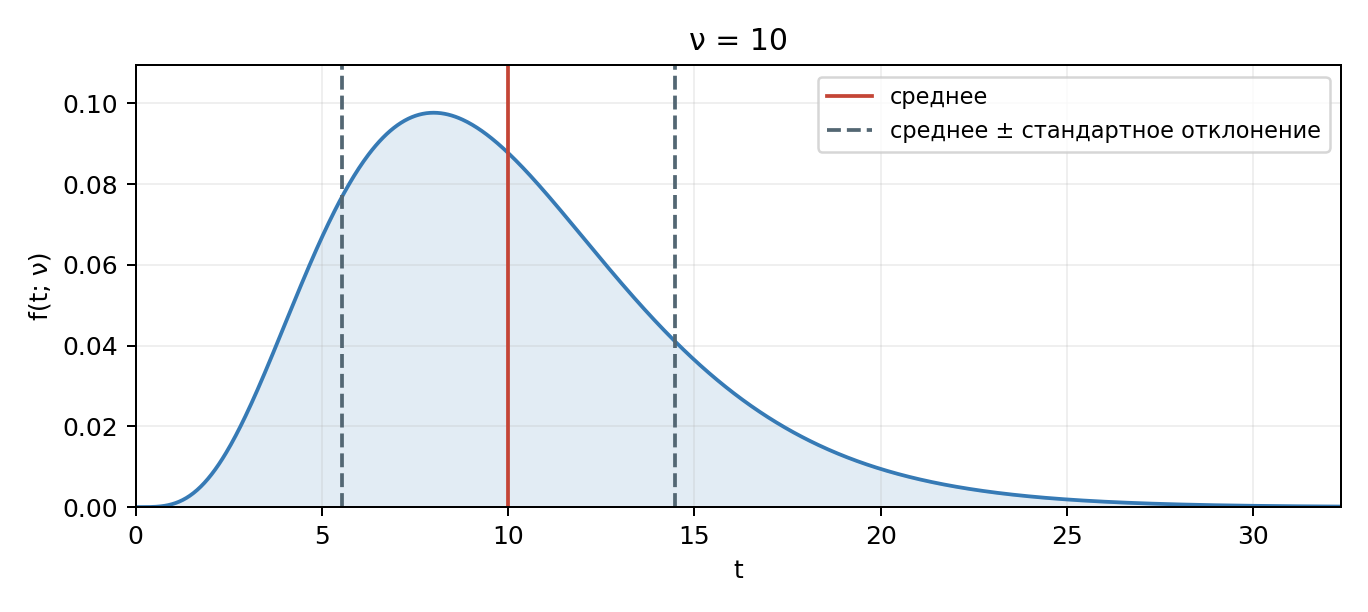
\includegraphics[width=0.74\linewidth,height=\textheight,keepaspectratio,alt={Форма распределения χ²}]{assets/figures/gof_chi2_nu10.png}

\end{center}

\noindent\begin{minipage}[c]{\dimexpr\linewidth-30mm\relax}

\textbf{Интерактив}. \textbf{Форма распределения χ²}

При \(\nu=10\) среднее равно \(10\), стандартное отклонение ---
\(\sqrt{20}\). Плотность асимметрична. Отметки среднего и ширины не
являются границами интервала с заданной вероятностью.

\end{minipage}\hfill\begin{minipage}[c]{26mm}\centering

\href{https://neutrinohit.github.io/statistical-analysis-course/ru/book/chapters/13_goodness_of_fit_and_significance.html\#interactive-goodness-chi2-shape}{
\includegraphics[width=24mm,height=\textheight,keepaspectratio,alt={QR-код интерактива}]{assets/qr/goodness-chi2-shape.png}}

\end{minipage}

\end{semanticpdfbox}

С ростом \(\nu\) распределение становится более симметричным. В
центральной области работает гауссово приближение
\((T-\nu)/\sqrt{2\nu}\approx\mathcal N(0,1)\). Для далёкого хвоста
точность этого приближения нужно проверять: именно там нас могут
интересовать вероятности порядка \(10^{-5}\) и меньше.

\section{Сколько степеней свободы осталось после
фита?}\label{ux441ux43aux43eux43bux44cux43aux43e-ux441ux442ux435ux43fux435ux43dux435ux439-ux441ux432ux43eux431ux43eux434ux44b-ux43eux441ux442ux430ux43bux43eux441ux44c-ux43fux43eux441ux43bux435-ux444ux438ux442ux430}

\subsection{Коррелированные
ошибки}\label{ux43aux43eux440ux440ux435ux43bux438ux440ux43eux432ux430ux43dux43dux44bux435-ux43eux448ux438ux431ux43aux438}

Пусть данные гауссовы, их средние \(\boldsymbol\lambda\) заданы заранее,
а ковариация \(V_y\) известна и положительно определена:

\begin{equation}\protect\phantomsection\label{eq-ch13-correlated-chi-square}{
\chi^2=
(\mathbf y-\boldsymbol\lambda)^{\mathsf T}
V_y^{-1}(\mathbf y-\boldsymbol\lambda).
}\end{equation}

Между измерениями могут быть сильные корреляции. Уменьшилось ли из-за
этого число независимых направлений? Проверим заменой координат.

Диагонализуем ковариацию и нормируем каждую координату на её ошибку:

\begin{equation}\protect\phantomsection\label{eq-ch13-whitened-coordinates}{
\begin{aligned}
V_y&=QDQ^{\mathsf T},
\qquad D=\operatorname{diag}(d_1,\ldots,d_N),\\
\mathbf g&=D^{-1/2}Q^{\mathsf T}
(\mathbf y-\boldsymbol\lambda).
\end{aligned}
}\end{equation}

Матрица \(Q\) ортогональна, все \(d_i>0\). В новых координатах
ковариация единичная. Для совместно гауссовых данных это означает
независимость компонент, и

\begin{equation}\protect\phantomsection\label{eq-ch13-correlated-distribution}{
\chi^2=\sum_{i=1}^{N}g_i^2\sim\chi^2_N.
}\end{equation}

Осталось ровно \(N\) направлений. Корреляции изменили их ориентацию и
масштабы. При вырожденной ковариации появляются точные ограничения:
тогда сначала выделяют допустимое подпространство. Обычной обратной
матрицы в формуле \ref{eq-ch13-correlated-chi-square} уже нет.

\subsection{Подгонка выбирает
проекцию}\label{ux43fux43eux434ux433ux43eux43dux43aux430-ux432ux44bux431ux438ux440ux430ux435ux442-ux43fux440ux43eux435ux43aux446ux438ux44e}

Для линейной модели \(X\boldsymbol\theta\) с \(m\) независимыми
параметрами предсказания образуют \(m\)-мерное линейное подпространство.
Здесь \(m\) --- ранг матрицы модели; два одинаковых столбца не дают двух
независимых параметров.

После преобразования \ref{eq-ch13-whitened-coordinates} подгонка
выбирает ближайшую точку подпространства модели. Остаток ортогонален ему
и имеет \(N-m\) независимых компонент. Если модель верна, все эти
компоненты стандартные гауссовы. Поэтому {[}1{]}

\begin{equation}\protect\phantomsection\label{eq-ch13-fitted-degrees-of-freedom}{
\chi^2_{\min}\sim\chi^2_\nu,
\qquad \nu=N-m.
}\end{equation}

Это точный результат для линейной гауссовой задачи с известной
ковариацией и свободными параметрами. Если истинный параметр лежит на
физической границе или модель существенно нелинейна, такая геометрия
может перестать работать.

\subsection{Куда уходит одна степень
свободы}\label{ux43aux443ux434ux430-ux443ux445ux43eux434ux438ux442-ux43eux434ux43dux430-ux441ux442ux435ux43fux435ux43dux44c-ux441ux432ux43eux431ux43eux434ux44b}

Для измерений одной величины с одинаковыми известными ошибками

\begin{equation}\protect\phantomsection\label{eq-ch13-common-mean}{
Y_i\sim\mathcal N(\mu,\sigma^2),
\qquad
\widehat\mu=\overline Y.
}\end{equation}

До подгонки сумма \(\sum_i(Y_i-\mu)^2/\sigma^2\) имеет \(N\) степеней
свободы. После подгонки \(\sum_i(Y_i-\overline Y)=0\): свободных
остатков стало на один меньше.

Это можно записать точным равенством

\begin{equation}\protect\phantomsection\label{eq-ch13-mean-decomposition}{
\sum_i\frac{(Y_i-\mu)^2}{\sigma^2}
=
\sum_i\frac{(Y_i-\overline Y)^2}{\sigma^2}
+\frac{N(\overline Y-\mu)^2}{\sigma^2}.
}\end{equation}

Последнее слагаемое --- квадрат одной стандартной гауссовой величины. В
гауссовой модели оно независимо от первой суммы справа. Подгонка убрала
одно направление, оставив \(\chi^2_{N-1}\).

У калибровочной прямой два независимых параметра, если энергии
источников не все одинаковы. Поэтому в наших двух калибровках
\(\nu=12-2=10\) и \(\nu=1002-2=1000\).

\subsection{А если есть калибровочные
ограничения?}\label{ux430-ux435ux441ux43bux438-ux435ux441ux442ux44c-ux43aux430ux43bux438ux431ux440ux43eux432ux43eux447ux43dux44bux435-ux43eux433ux440ux430ux43dux438ux447ux435ux43dux438ux44f}

В прошлой главе мы включали в правдоподобие вспомогательные измерения.
Их нужно учитывать и при проверке качества согласия. В линейной
гауссовой задаче с \(N\) основными и \(K\) независимыми вспомогательными
данными после подгонки \(r\) независимых параметров остаётся \(N+K-r\)
степеней свободы.

Например, общая неизвестная поправка калибровки добавляет один параметр,
но независимое измерение этой поправки добавляет одно наблюдение. Просто
вычесть параметр из прежнего \(N\) было бы неверно. Этот подсчёт
предполагает, что в повторяемом опыте флуктуируют и основные, и
вспомогательные данные. Для другой процедуры распределение минимума
проверяют отдельно.

\section{p-значение: какую вероятность мы
вычисляем?}\label{p-ux437ux43dux430ux447ux435ux43dux438ux435-ux43aux430ux43aux443ux44e-ux432ux435ux440ux43eux44fux442ux43dux43eux441ux442ux44c-ux43cux44b-ux432ux44bux447ux438ux441ux43bux44fux435ux43c}

Обозначим проверяемую гипотезу через \(H_0\). В калибровочном примере
она утверждает, что отклик линейный, ошибки гауссовы и их ковариация
задана верно. Параметры прямой подгоняются по данным.

Пусть получено \(t_{\mathrm{obs}}=\chi^2_{\min}\). Сумма квадратов тем
больше, чем сильнее остаточное расхождение. Поэтому берём правый хвост:

\begin{equation}\protect\phantomsection\label{eq-chi-square-p-value}{
p=P_{H_0}(T\ge t_{\mathrm{obs}})
=\int_{t_{\mathrm{obs}}}^{\infty}f(t;\nu)\,dt.
}\end{equation}

Спросим словами: если повторять эксперимент при верной \(H_0\), в какой
доле опытов получится сумма квадратов хотя бы такого размера?

Вопрос о вероятности самой гипотезы здесь не ставился. Поэтому из
\(p=0.03\) нельзя получить утверждение «вероятность модели равна 3\%»
или «модель неверна с вероятностью 97\%». Число относится к
распределению возможных результатов при заданной гипотезе.

Если нужен формальный критерий отклонения, заранее выбирают
\textbf{уровень значимости} \(\alpha\) и отклоняют \(H_0\) при
\(p\le\alpha\). Для точной непрерывной калибровки доля ложных отклонений
верной гипотезы будет равна \(\alpha\). Значение \(\alpha\) задаётся
правилом проверки, а \(p\) вычисляется по конкретным данным.

\subsection{Интерактив: площадь
хвоста}\label{interactive-goodness-pvalue-tail}

В апплете можно менять \(\nu\) и полученное значение
\(t_{\mathrm{obs}}\). При движении вертикальной линии вправо закрашенная
площадь уменьшается. Вероятность вычисляется по функции распределения;
точность числа не зависит от густоты точек на графике.

\begin{semanticpdfbox}[breakable=false]

\begin{center}

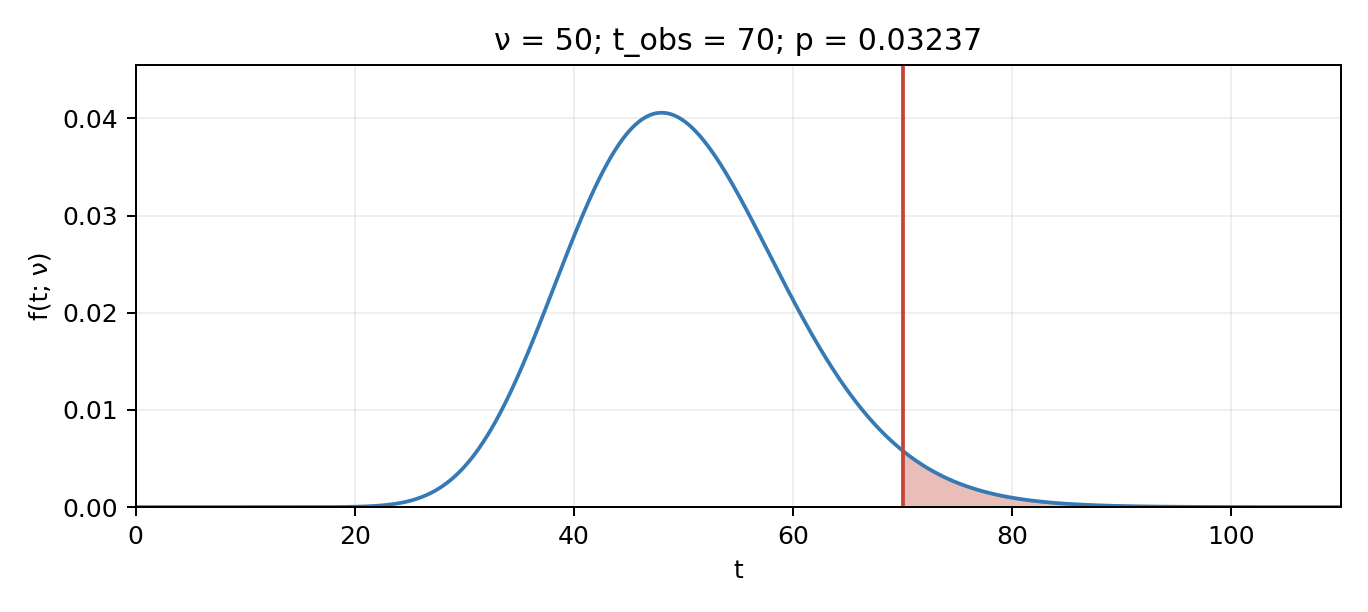
\includegraphics[width=0.74\linewidth,height=\textheight,keepaspectratio,alt={p-значение как площадь хвоста}]{assets/figures/gof_pvalue_nu50_obs70.png}

\end{center}

\noindent\begin{minipage}[c]{\dimexpr\linewidth-30mm\relax}

\textbf{Интерактив}. \textbf{p-значение как площадь хвоста}

Для \(\nu=50\) и \(t_{\mathrm{obs}}=70\) площадь правого хвоста равна
\(p\simeq0.0324\). Закрашена вероятность получить \(T\ge70\) при этой
модели.

\end{minipage}\hfill\begin{minipage}[c]{26mm}\centering

\href{https://neutrinohit.github.io/statistical-analysis-course/ru/book/chapters/13_goodness_of_fit_and_significance.html\#interactive-goodness-pvalue-tail}{
\includegraphics[width=24mm,height=\textheight,keepaspectratio,alt={QR-код интерактива}]{assets/qr/goodness-pvalue-tail.png}}

\end{minipage}

\end{semanticpdfbox}

Большое \(p\) означает, что выбранная статистика не обнаружила сильного
несогласия. Оно не устанавливает истинность модели: другая модель тоже
может описывать эти данные, а статистики может не хватить для различения
моделей.

Очень маленькое \(\chi^2\) тоже даёт повод проверить расчёт. Возможно,
ошибки завышены или часть данных была учтена несколько раз как
независимая. Но иногда малое значение возникает просто из-за флуктуации.
Правохвостовое \(p\), близкое к единице, само по себе не является
критерием для этой отдельной проверки.

\subsection{Как распределены сами
p-значения?}\label{interactive-goodness-pvalue-calibration}

Представим много опытов, в которых \(H_0\) верна. Для каждого вычислим
\(T\) и его p-значение. Если функция распределения \(F_0\) непрерывна,
то \(p=1-F_0(T)\). Преобразование переменной даёт

\begin{equation}\protect\phantomsection\label{eq-ch13-uniform-p-values}{
P_{H_0}(p\le u)=u,
\qquad 0\le u\le1.
}\end{equation}

Плотность p-значений равна единице на отрезке \([0,1]\). Значения около
\(0.5\) ничем не выделены. При пороге \(\alpha=0.05\) примерно каждый
двадцатый опыт с верной моделью попадёт в область отклонения.

В апплете одна выборка из \(\chi^2_{10}\) задаёт численную калибровку, а
независимая вторая выборка изображает повторные эксперименты. Число
опытов во второй выборке можно менять. Для каждого результата
подсчитывается правый хвост калибровочной выборки.

\begin{semanticpdfbox}[breakable=false]

\begin{center}

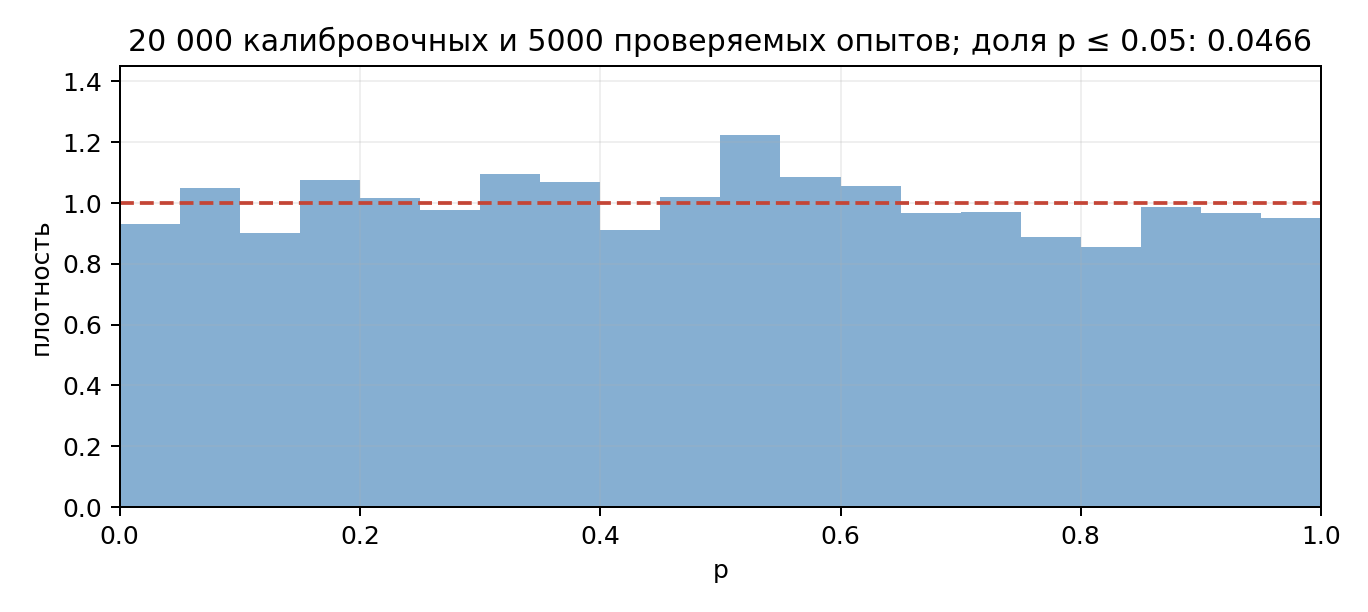
\includegraphics[width=0.74\linewidth,height=\textheight,keepaspectratio,alt={Распределение p-значений}]{assets/figures/gof_p_uniform.png}

\end{center}

\noindent\begin{minipage}[c]{\dimexpr\linewidth-30mm\relax}

\textbf{Интерактив}. \textbf{Распределение p-значений}

20 000 опытов задают калибровку; для 5000 независимых опытов построена
гистограмма p-значений. Пунктир показывает единичную плотность.
Отклонения столбцов связаны с конечным размером обеих выборок.

\end{minipage}\hfill\begin{minipage}[c]{26mm}\centering

\href{https://neutrinohit.github.io/statistical-analysis-course/ru/book/chapters/13_goodness_of_fit_and_significance.html\#interactive-goodness-pvalue-calibration}{
\includegraphics[width=24mm,height=\textheight,keepaspectratio,alt={QR-код интерактива}]{assets/qr/goodness-pvalue-calibration.png}}

\end{minipage}

\end{semanticpdfbox}

При конечной калибровочной выборке равномерность лишь приближённая. Для
дискретной статистики точное распределение p-значений также ступенчатое.
При определении через \(P(T\ge t_{\mathrm{obs}})\) получается
консервативное правило:

\begin{equation}\protect\phantomsection\label{eq-ch13-discrete-p-values}{
P_{H_0}(p\le\alpha)\le\alpha.
}\end{equation}

Например, при малом пуассоновском счёте может вообще не существовать
порога, дающего ровно 5\% ложных отклонений. Это свойство дискретных
данных, которое следует учитывать при чтении гистограммы p-значений.

\section{Возвращаемся к двум
калибровкам}\label{ux432ux43eux437ux432ux440ux430ux449ux430ux435ux43cux441ux44f-ux43a-ux434ux432ux443ux43c-ux43aux430ux43bux438ux431ux440ux43eux432ux43aux430ux43c}

Теперь вычислим интеграл \ref{eq-chi-square-p-value} для результатов из
начала главы. Для сравнения приведём и отклонение от среднего в единицах
ширины:

\begin{equation}\protect\phantomsection\label{eq-ch13-standardized-chi-square}{
z_{\chi^2}=\frac{t_{\mathrm{obs}}-\nu}{\sqrt{2\nu}}.
}\end{equation}

\begin{longtable}[]{@{}
  >{\raggedleft\arraybackslash}p{(\linewidth - 8\tabcolsep) * \real{0.1800}}
  >{\raggedleft\arraybackslash}p{(\linewidth - 8\tabcolsep) * \real{0.1400}}
  >{\raggedleft\arraybackslash}p{(\linewidth - 8\tabcolsep) * \real{0.2200}}
  >{\raggedleft\arraybackslash}p{(\linewidth - 8\tabcolsep) * \real{0.1800}}
  >{\raggedleft\arraybackslash}p{(\linewidth - 8\tabcolsep) * \real{0.2800}}@{}}
\caption{Два результата калибровки с одинаковым отношением
χ²/ν}\label{tbl-chi2-ratio-examples}\tabularnewline
\toprule\noalign{}
\begin{minipage}[b]{\linewidth}\raggedleft
\(t_{\mathrm{obs}}\)
\end{minipage} & \begin{minipage}[b]{\linewidth}\raggedleft
\(\nu\)
\end{minipage} & \begin{minipage}[b]{\linewidth}\raggedleft
\(t_{\mathrm{obs}}/\nu\)
\end{minipage} & \begin{minipage}[b]{\linewidth}\raggedleft
\(z_{\chi^2}\)
\end{minipage} & \begin{minipage}[b]{\linewidth}\raggedleft
\(p\)
\end{minipage} \\
\midrule\noalign{}
\endfirsthead
\toprule\noalign{}
\begin{minipage}[b]{\linewidth}\raggedleft
\(t_{\mathrm{obs}}\)
\end{minipage} & \begin{minipage}[b]{\linewidth}\raggedleft
\(\nu\)
\end{minipage} & \begin{minipage}[b]{\linewidth}\raggedleft
\(t_{\mathrm{obs}}/\nu\)
\end{minipage} & \begin{minipage}[b]{\linewidth}\raggedleft
\(z_{\chi^2}\)
\end{minipage} & \begin{minipage}[b]{\linewidth}\raggedleft
\(p\)
\end{minipage} \\
\midrule\noalign{}
\endhead
\bottomrule\noalign{}
\endlastfoot
\(12\) & \(10\) & \(1.20\) & \(0.447\) & \(0.2851\) \\
\(1200\) & \(1000\) & \(1.20\) & \(4.472\) & \(1.226\cdot10^{-5}\) \\
\end{longtable}

Первая калибровка не вызывает возражений по этой проверке. Во второй
остатки слишком велики для принятой модели ошибок. Нужно смотреть, где
именно возникло расхождение: кривизна отклика, отдельная точка,
зависимость ошибки от энергии, забытая общая систематика.

Само p-значение не выбирает причину. Оно относится ко всей проверяемой
модели, включая ошибки. Если увеличить все \(\sigma_i\), то χ²
уменьшится. Но подбирать ошибки так, чтобы отношение стало единицей, ---
значит менять исходную постановку по результату этой же проверки.

Поэтому запись результата должна сохранять оба числа:

\begin{equation}\protect\phantomsection\label{eq-ch13-report-fit}{
\chi^2_{\min}/\mathrm{ndf}=1200/1000,
\qquad p=1.226\cdot10^{-5}.
}\end{equation}

Сокращение \emph{ndf} означает число степеней свободы. Одна запись
«χ²/ndf = 1.2» теряет информацию, от которой зависит вывод.

\section{Что означает «число
сигма»?}\label{ux447ux442ux43e-ux43eux437ux43dux430ux447ux430ux435ux442-ux447ux438ux441ux43bux43e-ux441ux438ux433ux43cux430}

\subsection{Один хвост}\label{interactive-goodness-p-to-z-one-sided}

Малую хвостовую вероятность удобно перевести на знакомую гауссову шкалу.
Для стандартной гауссовой величины \(G\) определим число \(Z\) условием

\begin{equation}\protect\phantomsection\label{eq-ch13-one-sided-significance}{
p=P(G\ge Z)=1-\Phi(Z),
\qquad Z=\Phi^{-1}(1-p).
}\end{equation}

Функция \(\Phi\) --- функция распределения \(\mathcal N(0,1)\). Это
соглашение о представлении вероятности. Исходные данные могут быть
пуассоновскими, а статистика --- иметь распределение χ². Гауссовой здесь
служит шкала, на которую мы переводим уже найденное \(p\).

Для второго результата в таблице \ref{tbl-chi2-ratio-examples}
односторонний перевод даёт \(Z\simeq4.22\). Число \(z_{\chi^2}=4.472\) в
той же таблице другое: оно получено вычитанием среднего и делением на
стандартное отклонение. У асимметричного распределения эта операция не
воспроизводит точную вероятность хвоста.

\begin{semanticpdfbox}[breakable=false]

\begin{center}

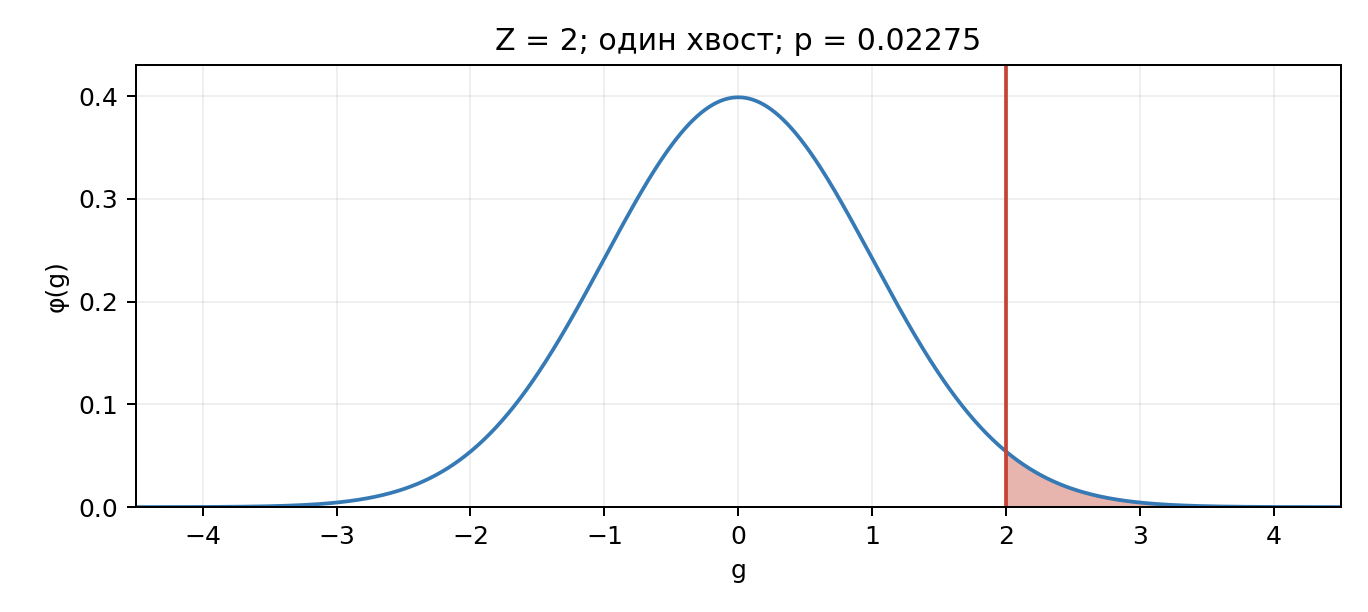
\includegraphics[width=0.74\linewidth,height=\textheight,keepaspectratio,alt={Односторонняя гауссова шкала}]{assets/figures/gof_p_to_z_one_sided.png}

\end{center}

\noindent\begin{minipage}[c]{\dimexpr\linewidth-30mm\relax}

\textbf{Интерактив}. \textbf{Односторонняя гауссова шкала}

При \(Z=2\) правый хвост содержит \(p=0.02275\). Ползунок в HTML
позволяет сопоставить положение границы с площадью хвоста.

\end{minipage}\hfill\begin{minipage}[c]{26mm}\centering

\href{https://neutrinohit.github.io/statistical-analysis-course/ru/book/chapters/13_goodness_of_fit_and_significance.html\#interactive-goodness-p-to-z-one-sided}{
\includegraphics[width=24mm,height=\textheight,keepaspectratio,alt={QR-код интерактива}]{assets/qr/goodness-p-to-z-one-sided.png}}

\end{minipage}

\end{semanticpdfbox}

\begin{longtable}[]{@{}rr@{}}
\caption{Одностороннее соответствие p и
Z}\label{tbl-p-to-z-one-sided}\tabularnewline
\toprule\noalign{}
\(Z\) & \(p=1-\Phi(Z)\) \\
\midrule\noalign{}
\endfirsthead
\toprule\noalign{}
\(Z\) & \(p=1-\Phi(Z)\) \\
\midrule\noalign{}
\endhead
\bottomrule\noalign{}
\endlastfoot
\(1\) & \(1.587\cdot10^{-1}\) \\
\(2\) & \(2.275\cdot10^{-2}\) \\
\(3\) & \(1.350\cdot10^{-3}\) \\
\(4\) & \(3.167\cdot10^{-5}\) \\
\(5\) & \(2.867\cdot10^{-7}\) \\
\end{longtable}

При поиске положительного сигнала обычно используют именно такое
соглашение. Порог открытия \(5\sigma\) соответствует правому хвосту из
таблицы \ref{tbl-p-to-z-one-sided}. Если \(p>1/2\), формула
\ref{eq-ch13-one-sided-significance} даёт отрицательное \(Z\). Такое
число не означает свидетельства в пользу положительного сигнала.

\subsection{Два хвоста}\label{interactive-goodness-p-to-z-two-sided}

Если нас интересуют отклонения от заданного значения в обе стороны,
складываются две хвостовые вероятности:

\begin{equation}\protect\phantomsection\label{eq-ch13-two-sided-significance}{
p=P(|G|\ge Z)=2[1-\Phi(Z)],
\qquad Z=\Phi^{-1}(1-p/2),\quad Z\ge0.
}\end{equation}

Для \(Z=2\) теперь получается \(p=0.04550\), вдвое больше одностороннего
значения. Выбор определяется вопросом анализа. Его нельзя менять после
того, как стал известен знак отклонения.

\begin{semanticpdfbox}[breakable=false]

\begin{center}

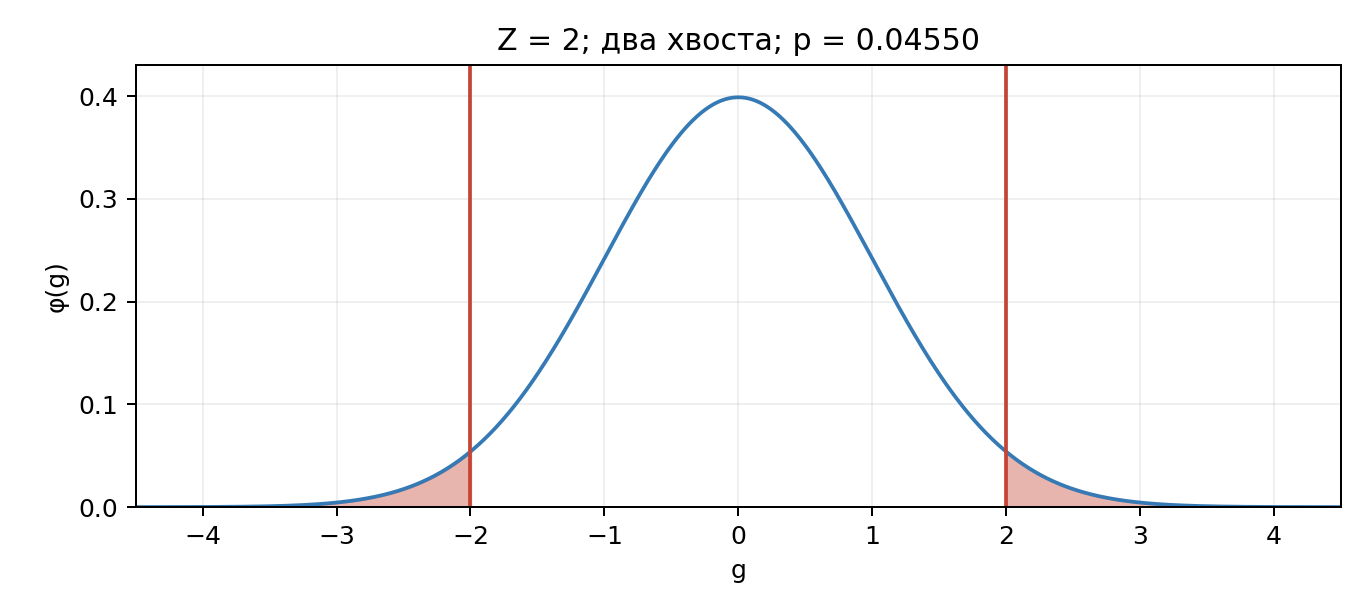
\includegraphics[width=0.74\linewidth,height=\textheight,keepaspectratio,alt={Два гауссовых хвоста}]{assets/figures/gof_p_to_z_two_sided.png}

\end{center}

\noindent\begin{minipage}[c]{\dimexpr\linewidth-30mm\relax}

\textbf{Интерактив}. \textbf{Два гауссовых хвоста}

За пределами \([-2,2]\) находится вероятность \(0.04550\). Каждый из
двух хвостов содержит половину этой вероятности.

\end{minipage}\hfill\begin{minipage}[c]{26mm}\centering

\href{https://neutrinohit.github.io/statistical-analysis-course/ru/book/chapters/13_goodness_of_fit_and_significance.html\#interactive-goodness-p-to-z-two-sided}{
\includegraphics[width=24mm,height=\textheight,keepaspectratio,alt={QR-код интерактива}]{assets/qr/goodness-p-to-z-two-sided.png}}

\end{minipage}

\end{semanticpdfbox}

Уже знакомый интервал для одного параметра в квадратичном приближении
строится из

\begin{equation}\protect\phantomsection\label{eq-ch13-parameter-significance}{
\Delta\chi^2(\theta)
\simeq\frac{(\theta-\widehat\theta)^2}{\sigma_\theta^2}.
}\end{equation}

Его границы \(\widehat\theta\pm Z\sigma_\theta\) соответствуют
\(\Delta\chi^2=Z^2\). В точной линейной гауссовой задаче покрытие такого
интервала равно \(2\Phi(Z)-1\).

\begin{longtable}[]{@{}
  >{\raggedright\arraybackslash}p{(\linewidth - 4\tabcolsep) * \real{0.2571}}
  >{\raggedleft\arraybackslash}p{(\linewidth - 4\tabcolsep) * \real{0.3571}}
  >{\raggedleft\arraybackslash}p{(\linewidth - 4\tabcolsep) * \real{0.3857}}@{}}
\caption{Двусторонние гауссовы интервалы одного
параметра}\label{tbl-p-to-z-two-sided}\tabularnewline
\toprule\noalign{}
\begin{minipage}[b]{\linewidth}\raggedright
Границы интервала
\end{minipage} & \begin{minipage}[b]{\linewidth}\raggedleft
Вероятность двух хвостов
\end{minipage} & \begin{minipage}[b]{\linewidth}\raggedleft
\(\Delta\chi^2\) на границе
\end{minipage} \\
\midrule\noalign{}
\endfirsthead
\toprule\noalign{}
\begin{minipage}[b]{\linewidth}\raggedright
Границы интервала
\end{minipage} & \begin{minipage}[b]{\linewidth}\raggedleft
Вероятность двух хвостов
\end{minipage} & \begin{minipage}[b]{\linewidth}\raggedleft
\(\Delta\chi^2\) на границе
\end{minipage} \\
\midrule\noalign{}
\endhead
\bottomrule\noalign{}
\endlastfoot
\(\widehat\theta\pm\sigma_\theta\) & \(3.173\cdot10^{-1}\) & \(1\) \\
\(\widehat\theta\pm2\sigma_\theta\) & \(4.550\cdot10^{-2}\) & \(4\) \\
\(\widehat\theta\pm3\sigma_\theta\) & \(2.700\cdot10^{-3}\) & \(9\) \\
\(\widehat\theta\pm4\sigma_\theta\) & \(6.334\cdot10^{-5}\) & \(16\) \\
\(\widehat\theta\pm5\sigma_\theta\) & \(5.733\cdot10^{-7}\) & \(25\) \\
\end{longtable}

Это утверждение относится к приращению функции для одного параметра.
Подставлять вместо него полное \(\chi^2_{\min}\) нельзя.

\section{Читаем графики поиска бозона
Хиггса}\label{ux447ux438ux442ux430ux435ux43c-ux433ux440ux430ux444ux438ux43aux438-ux43fux43eux438ux441ux43aux430-ux431ux43eux437ux43eux43dux430-ux445ux438ux433ux433ux441ux430}

Вернёмся к рисункам из первой главы. По горизонтали стоит пробная масса
\(m_H\), по вертикали --- локальное p-значение фоновой гипотезы. В
каждой точке спрашивают: как часто один фон даёт избыток, настолько же
похожий на сигнал с этой массой?

\begin{figure}[H]

\centering{

\pandocbounded{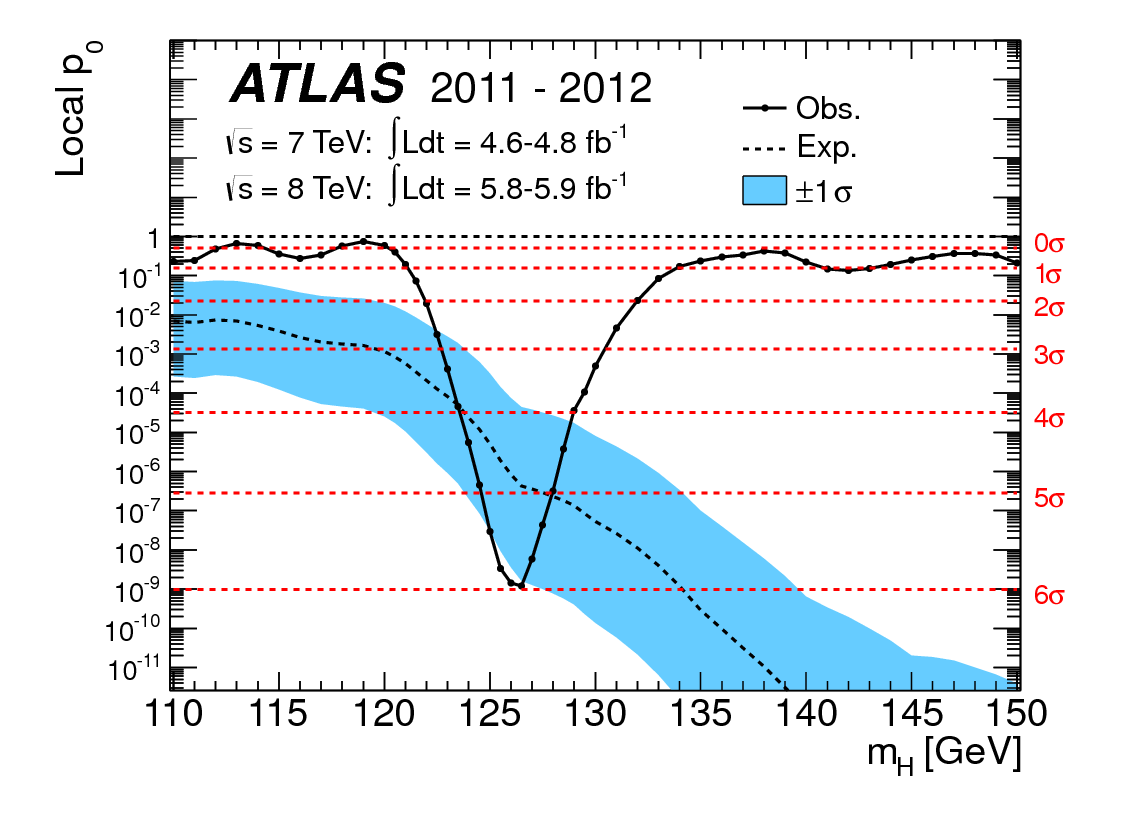
\includegraphics[keepaspectratio]{chapters/../assets/figures/gof_atlas_pvalue.png}}

}

\caption{\label{fig-goodness-atlas-pvalue}Локальное p-значение фоновой
гипотезы в ATLAS. Сплошная чёрная кривая получена из данных; пунктир и
голубая полоса относятся к ожидаемому результату при наличии бозона
Хиггса Стандартной модели с пробной массой. Рисунок из статьи ATLAS
{[}2{]}.}

\end{figure}%

На рисунке \ref{fig-goodness-atlas-pvalue} минимум около \(126\) ГэВ
достигает локальной значимости \(5.9\sigma\). Вертикальная шкала
логарифмическая. Красные линии переводят её в односторонние \(Z\): чем
глубже минимум p-значения, тем сильнее несогласие с фоном.

Пунктирная кривая отвечает другому расчёту: какой результат ожидается,
если сигнал Стандартной модели действительно есть при каждой проверяемой
массе. Она не является подгонкой чёрной кривой.

\begin{figure}[H]

\centering{

\pandocbounded{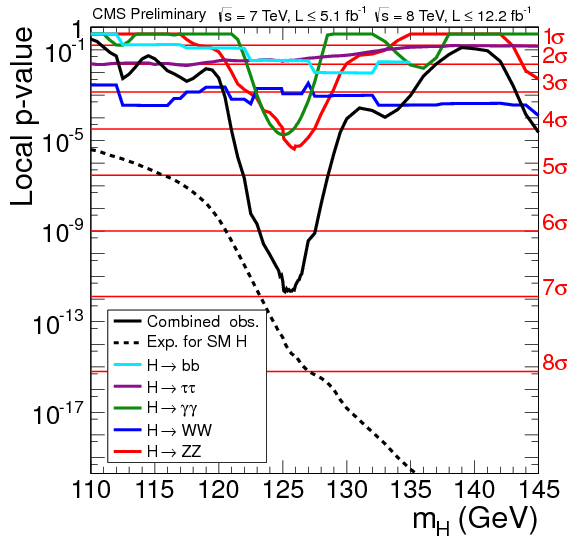
\includegraphics[keepaspectratio]{chapters/../assets/figures/gof_cms_pvalue.png}}

}

\caption{\label{fig-goodness-cms-pvalue}Локальные p-значения в
предварительном результате CMS с данными при 7 и 8 ТэВ и светимостью до
12.2 фб\(^{-1}\) при 8 ТэВ. Цветные кривые показывают отдельные каналы
распада, чёрная --- их объединение. Источник: CMS PAS HIG-12-045
{[}3{]}.}

\end{figure}%

В первой статье об открытии CMS сообщала локальную значимость
\(5.0\sigma\) {[}4{]}. На рисунке \ref{fig-goodness-cms-pvalue}
используется уже больший набор данных, и минимум стал глубже. Сравнивая
результаты, нужно проверять накопленную светимость и версию анализа:
число сигма относится к конкретной выборке.

Обе иллюстрации относятся к проверке \textbf{фоновой гипотезы}. Качество
согласия модели «сигнал плюс фон» с данными проверяется отдельно. Малое
p-значение фона само по себе не сообщает, насколько подробно выбранная
модель сигнала описывает все свойства событий.

\subsection{Локальный результат и поиск по
массе}\label{ux43bux43eux43aux430ux43bux44cux43dux44bux439-ux440ux435ux437ux443ux43bux44cux442ux430ux442-ux438-ux43fux43eux438ux441ux43a-ux43fux43e-ux43cux430ux441ux441ux435}

При фиксированной заранее массе получается локальное p-значение. Если
массу выбирали по самому глубокому минимуму в диапазоне, в повторяемом
опыте нужно каждый раз просматривать весь этот диапазон. Так
определяется глобальное p-значение: вероятность найти где-либо в нём
столь же сильное отклонение {[}5{]}.

Соседние массы проверяются по одним и тем же данным, поэтому их
результаты коррелированы. Число точек на нарисованной кривой не равно
числу независимых попыток.

\subsection{\texorpdfstring{Откуда возникает правило
\(Z=\sqrt{q_0}\)}{Откуда возникает правило Z=\textbackslash sqrt\{q\_0\}}}\label{ux43eux442ux43aux443ux434ux430-ux432ux43eux437ux43dux438ux43aux430ux435ux442-ux43fux440ux430ux432ux438ux43bux43e-zsqrtq_0}

Покажем его на простой гауссовой модели. Пусть измеряется амплитуда
сигнала \(Y\sim\mathcal N(s,\sigma^2)\), где \(\sigma\) известна, а
физически \(s\ge0\). Проверяется фон \(s=0\). Подгонка с ограничением
даёт \(\widehat s=\max(0,y)\). Улучшение суммы квадратов равно

\begin{equation}\protect\phantomsection\label{eq-ch13-discovery-statistic}{
q_0=\chi^2(0)-\chi^2(\widehat s)
=
\begin{cases}
y^2/\sigma^2,&y>0,\\
0,&y\le0.
\end{cases}
}\end{equation}

При верном фоне половина опытов имеет \(Y\le0\) и даёт \(q_0=0\).
Положительная часть соответствует половине распределения \(\chi^2_1\).
Для полученного \(q_0>0\) имеем

\begin{equation}\protect\phantomsection\label{eq-ch13-discovery-significance}{
p_0=P_{s=0}(q_0(Y)\ge q_0)
=1-\Phi(\sqrt{q_0}),
\qquad Z=\sqrt{q_0}.
}\end{equation}

Поэтому \(q_0=25\) даёт односторонние \(5\sigma\). Для чистого
\(\chi^2_1\) вероятность правее 25 вдвое больше: квадрат учитывает оба
знака исходного гауссова отклонения.

В задачах поиска частиц аналогичная формула возникает как асимптотика
профильной статистики при одном неотрицательном параметре сигнала и
выполнении соответствующих условий регулярности {[}5{]}. К произвольному
минимуму χ² она не относится.

\section{Когда распределение нужно получить
моделированием}\label{ux43aux43eux433ux434ux430-ux440ux430ux441ux43fux440ux435ux434ux435ux43bux435ux43dux438ux435-ux43dux443ux436ux43dux43e-ux43fux43eux43bux443ux447ux438ux442ux44c-ux43cux43eux434ux435ux43bux438ux440ux43eux432ux430ux43dux438ux435ux43c}

\subsection{Малые пуассоновские
счёты}\label{ux43cux430ux43bux44bux435-ux43fux443ux430ux441ux441ux43eux43dux43eux432ux441ux43aux438ux435-ux441ux447ux451ux442ux44b}

Рассмотрим пример из лекции: двадцать независимых пуассоновских бинов с
заранее заданными ожиданиями \(\mu_i\). Здесь нет подгоняемых параметров
и не фиксируется суммарное число событий:

\begin{equation}\protect\phantomsection\label{eq-ch13-pearson-statistic}{
N_i\sim\operatorname{Pois}(\mu_i),
\qquad
T_{\mathrm P}=\sum_{i=1}^{20}\frac{(N_i-\mu_i)^2}{\mu_i}.
}\end{equation}

Это \textbf{статистика Пирсона}. При больших ожиданиях каждое
\((N_i-\mu_i)/\sqrt{\mu_i}\) приближается к стандартной гауссовой
величине, и сумма квадратов приближённо имеет распределение
\(\chi^2_{20}\). Но в примере ожидания малы:

\begin{longtable}[]{@{}lrlr@{}}
\caption{Ожидаемые числа событий в двадцати
бинах}\label{tbl-ch13-small-poisson-means}\tabularnewline
\toprule\noalign{}
Бины & \(\mu_i\) & Бины & \(\mu_i\) \\
\midrule\noalign{}
\endfirsthead
\toprule\noalign{}
Бины & \(\mu_i\) & Бины & \(\mu_i\) \\
\midrule\noalign{}
\endhead
\bottomrule\noalign{}
\endlastfoot
1, 20 & 0.158 & 6, 15 & 1.785 \\
2, 19 & 0.295 & 7, 14 & 2.355 \\
3, 18 & 0.513 & 8, 13 & 2.899 \\
4, 17 & 0.833 & 9, 12 & 3.330 \\
5, 16 & 1.263 & 10, 11 & 3.568 \\
\end{longtable}

У статистики \ref{eq-ch13-pearson-statistic} среднее всё равно равно 20.
Для каждого бина \(\mathbb E[(N_i-\mu_i)^2]=\mu_i\). Но совпадения
среднего недостаточно, чтобы совпало распределение. Используя
центральный четвёртый момент Пуассона
\(\mathbb E[(N_i-\mu_i)^4]=\mu_i+3\mu_i^2\), получаем

\begin{equation}\protect\phantomsection\label{eq-ch13-pearson-variance}{
\operatorname{Var}(T_{\mathrm P})
=\sum_{i=1}^{20}\left(2+\frac{1}{\mu_i}\right)
\simeq71.14.
}\end{equation}

У \(\chi^2_{20}\) дисперсия равна 40. Уже по ширине видно, что
аналитическая замена неточна. Малые \(\mu_i\) дают особенно большой
добавочный вклад.

\subsection{Интерактив: распределение из
опытов}\label{interactive-goodness-low-count-calibration}

Для каждого опыта генерируем двадцать счётов из заданных пуассоновских
распределений и вычисляем ту же сумму Пирсона. Полученные значения
задают распределение \(T_{\mathrm P}\) при нашей модели.

Ползунок задаёт проверяемое значение \(t_{\mathrm{obs}}\). При
\(t_{\mathrm{obs}}=29.8\) независимая проверка на миллионе опытов даёт
\(p\simeq0.113\) со статистической ошибкой моделирования около
\(0.0003\). Формула для \(\chi^2_{20}\) даёт \(0.07316\). Апплет
использует 80 000 опытов, поэтому последняя цифра его результата может
отличаться.

\begin{semanticpdfbox}[breakable=false]

\begin{center}

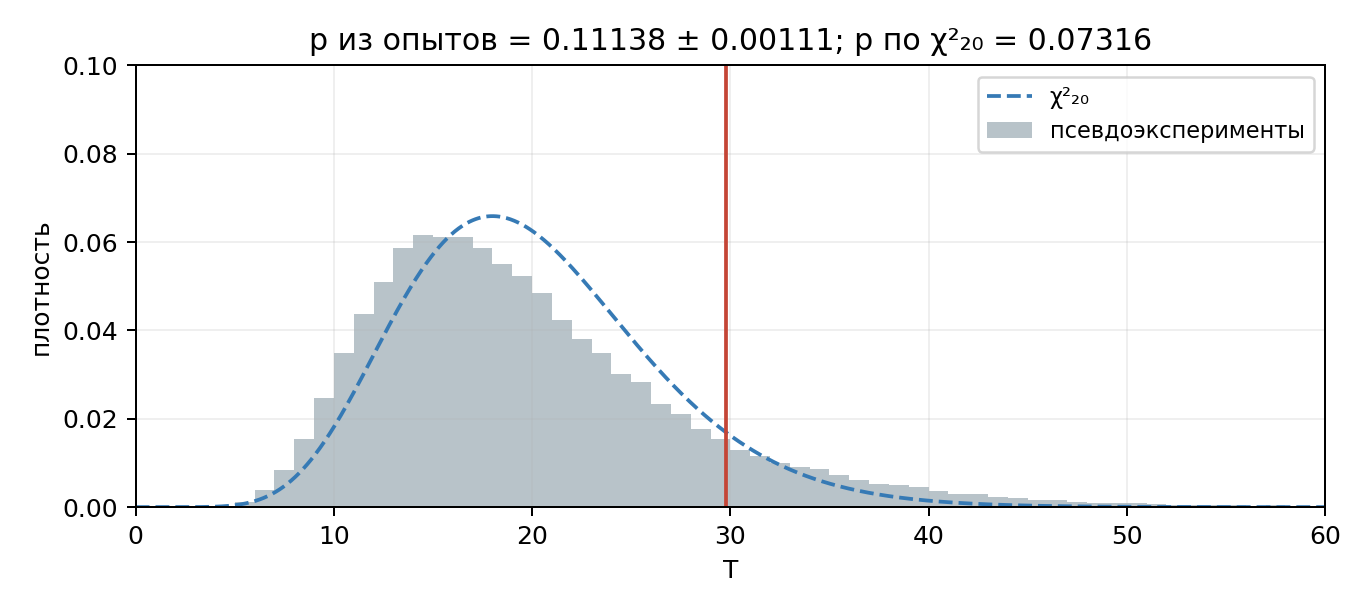
\includegraphics[width=0.74\linewidth,height=\textheight,keepaspectratio,alt={Проверка χ²-приближения при малых счётах}]{assets/figures/gof_low_count_toys.png}

\end{center}

\noindent\begin{minipage}[c]{\dimexpr\linewidth-30mm\relax}

\textbf{Интерактив}. \textbf{Проверка χ²-приближения при малых счётах}

Гистограмма построена по 80 000 опытов для ожиданий из таблицы
\ref{tbl-ch13-small-poisson-means}. Пунктир --- плотность
\(\chi^2_{20}\), вертикальная линия --- \(t_{\mathrm{obs}}=29.8\). Оба
p-значения вычисляются по всему хвосту, включая значения за правой
границей рисунка.

\end{minipage}\hfill\begin{minipage}[c]{26mm}\centering

\href{https://neutrinohit.github.io/statistical-analysis-course/ru/book/chapters/13_goodness_of_fit_and_significance.html\#interactive-goodness-low-count-calibration}{
\includegraphics[width=24mm,height=\textheight,keepaspectratio,alt={QR-код интерактива}]{assets/qr/goodness-low-count-calibration.png}}

\end{minipage}

\end{semanticpdfbox}

Можно выбрать другую статистику, например отношение пуассоновских
правдоподобий к насыщенной модели. В насыщенной модели для каждого бина
разрешено отдельное среднее, и его оценка равна \(n_i\):

\begin{equation}\protect\phantomsection\label{eq-ch13-poisson-likelihood-ratio}{
T_{\mathrm L}
=2\sum_i\left[
\mu_i-n_i+n_i\ln\frac{n_i}{\mu_i}
\right].
}\end{equation}

При \(n_i=0\) логарифмическое слагаемое по пределу равно нулю. Если
\(n_i\) близко к \(\mu_i\), разложение логарифма даёт статистику Пирсона
в ведущем квадратичном порядке. При малых счётах обе статистики
определены, но имеют разные распределения. Само использование
правдоподобия не делает распределение
\ref{eq-ch13-poisson-likelihood-ratio} точно равным χ² при любом числе
событий.

\subsection{Что повторять в
псевдоэксперименте}\label{ux447ux442ux43e-ux43fux43eux432ux442ux43eux440ux44fux442ux44c-ux432-ux43fux441ux435ux432ux434ux43eux44dux43aux441ux43fux435ux440ux438ux43cux435ux43dux442ux435}

Если параметры подгонялись по данным, то и в каждом псевдоэксперименте
их нужно подгонять заново. Если в анализ входили вспомогательные
калибровки, отбор событий или поиск по диапазону масс, процедура
калибровки статистики должна учитывать эти действия.

При полностью заданной гипотезе \(H_0\) доля превышений оценивается как

\begin{equation}\protect\phantomsection\label{eq-ch13-monte-carlo-p-value}{
\widehat p=\frac{k}{B},
\qquad
\sigma_{\widehat p}\simeq
\sqrt{\frac{\widehat p(1-\widehat p)}{B}},
}\end{equation}

где \(B\) --- число независимых опытов, \(k\) --- число значений
\(T\ge t_{\mathrm{obs}}\). Формула ошибки годится, когда превышений и
непревышений достаточно много. Если \(k=0\), нулевая оценка ошибки по
этой формуле бессодержательна: редкий хвост просто не разрешён данной
выборкой. При \(p\simeq2.9\cdot10^{-7}\) даже миллион опытов даёт в
среднем меньше одного превышения.

Для численного рангового теста с конечной калибровочной выборкой часто
используют \((k+1)/(B+1)\), включая сам проверяемый результат в набор из
\(B+1\) равноценных реализаций. Именно так устроен апплет распределения
p-значений выше. Этот приём не заменяет проверку модели и не устраняет
неопределённость редкого хвоста.

Если \(H_0\) содержит неизвестные параметры, остаётся вопрос, при каких
значениях генерировать опыты. Подстановка найденных оценок даёт
распространённую приближённую калибровку. Её частотные свойства нужно
проверять по допустимым значениям мешающих параметров. Одна генерация
при наилучшем фите не гарантирует правильный уровень для всей составной
гипотезы.

\begin{bookchaptersummary}[Итоги главы]

\begin{itemize}
\tightlist
\item
  В линейной гауссовой задаче с известной ковариацией минимум χ² имеет
  \(N-m\) степеней свободы. Корреляции учитываются ковариацией; подгонка
  уменьшает размерность пространства остатков.
\item
  p-значение --- хвостовая вероятность выбранной статистики при
  проверяемой гипотезе. Отношение χ²/ν без самого ν не определяет эту
  вероятность.
\item
  «Число сигма» задаёт гауссово представление p-значения. Один и два
  хвоста, проверка фона и качество фита требуют разных постановок; их
  нельзя смешивать.
\item
  При неточной аналитической калибровке распределение статистики
  получают псевдоэкспериментами с той же процедурой анализа. Число
  опытов ограничивает точность вычисления редких хвостов.
\end{itemize}

\end{bookchaptersummary}

\section{Задачи}\label{ux437ux430ux434ux430ux447ux438-12}

\begin{semanticpdfbox}[colback=BookCoralSoft,borderline west={1.2mm}{0pt}{BookCoral},breakable=false]

\noindent{\sffamily\bfseries\fontsize{11.2}{13.5}\selectfont Задача 1. Две статистики для пуассоновских бинов}\par\nopagebreak[4]\vspace{1.2mm}

В двадцати независимых бинах \(N_i\sim\operatorname{Pois}(\mu_i)\).
Первые десять ожиданий равны
\((0.158,0.295,0.513,0.833,1.263,1.785,2.355,2.899,3.330,3.568)\),
остальные заданы симметрией \(\mu_{21-i}=\mu_i\). Все ожидания известны;
параметры по данным не подгоняются.

\begin{enumerate}
\def\labelenumi{\arabic{enumi}.}
\tightlist
\item
  Запишите статистику Пирсона и выведите статистику отношения
  правдоподобий к насыщенной модели, где каждому бину разрешено своё
  среднее.
\item
  Разложите логарифм при \(n_i=\mu_i+\delta_i\), \(|\delta_i|\ll\mu_i\).
  Сравните ведущие квадратичные члены.
\item
  Найдите вклады пустого бина в обе статистики. Почему малое число
  событий само по себе не мешает вычислить эти вклады?
\item
  Выведите среднее и дисперсию статистики Пирсона, используя
  \(\mathbb E[(N_i-\mu_i)^4]=\mu_i+3\mu_i^2\).
\item
  Сгенерируйте 50 000 опытов. Сравните распределения обеих статистик с
  \(\chi^2_{20}\). Повторите при увеличении всех \(\mu_i\) в 100 раз.
\end{enumerate}

\end{semanticpdfbox}

\begin{semanticpdfbox}[colback=BookCoralSoft,borderline west={1.2mm}{0pt}{BookCoral},breakable=false]

\noindent{\sffamily\bfseries\fontsize{11.2}{13.5}\selectfont Задача 2. Степени свободы до и после подгонки}\par\nopagebreak[4]\vspace{1.2mm}

Даны \(N=12\) независимых измерений \(Y_i\sim\mathcal N(\mu,\sigma^2)\)
при \(\mu=10\) каналах и известной \(\sigma=2\) канала. Проведите 20 000
псевдоэкспериментов.

\begin{enumerate}
\def\labelenumi{\arabic{enumi}.}
\tightlist
\item
  В каждом опыте вычислите среднее \(\overline Y\), сумму квадратов
  относительно истинного \(\mu\) и минимальную сумму квадратов
  относительно \(\overline Y\); ошибки в знаменателях равны \(\sigma\).
\item
  Проверьте точное разложение суммы квадратов на два слагаемых: минимум
  и \(N(\overline Y-\mu)^2/\sigma^2\).
\item
  Сравните три распределения с \(\chi^2_{12}\), \(\chi^2_{11}\) и
  \(\chi^2_1\). Проверьте их средние и дисперсии.
\item
  Объясните, почему остатки после подгонки не являются двенадцатью
  независимыми стандартными гауссовыми величинами.
\item
  Найдите p-значение для \(\chi^2_{\min}=12\). Что получится, если
  ошибочно оставить двенадцать степеней свободы?
\end{enumerate}

\end{semanticpdfbox}

\begin{semanticpdfbox}[colback=BookCoralSoft,borderline west={1.2mm}{0pt}{BookCoral},breakable=false]

\noindent{\sffamily\bfseries\fontsize{11.2}{13.5}\selectfont Задача 3. Одинаковый χ² и разная форма остатков}\par\nopagebreak[4]\vspace{1.2mm}

Построим два учебных набора калибровочных данных. Энергии \(E_i=i\) МэВ,
\(i=0,\ldots,11\), ошибки амплитуды --- по 5 каналов. Матрица \(X\)
содержит столбцы \(1\) и \(E_i\).

Для первого набора сгенерируйте двенадцать независимых чисел
\(w_i\sim\mathcal N(0,1)\) и удалите их проекцию на прямую:
\(\mathbf v=\mathbf w-X(X^{\mathsf T}X)^{-1}X^{\mathsf T}\mathbf w\).
Для второго положите \(v_i=(E_i-5.5)^2-\tfrac1{12}\sum_j(E_j-5.5)^2\),
используя числовые значения энергий в МэВ. В каждом случае нормируйте
остаток: \(\mathbf u=\sqrt{12}\,\mathbf v/\|\mathbf v\|\), и задайте
амплитуды \(y_i=2+100E_i+5u_i\) в каналах.

\begin{enumerate}
\def\labelenumi{\arabic{enumi}.}
\tightlist
\item
  Подгоните оба набора прямой с двумя свободными параметрами.
\item
  Проверьте, что в обоих случаях \(\chi^2_{\min}=12\) и p-значения
  совпадают.
\item
  Постройте нормированные остатки по энергии. Какую особенность второго
  набора скрывает одно число χ²?
\item
  Объясните, почему эти специально сконструированные наборы нельзя
  использовать как случайную выборку для проверки распределения
  \(\chi^2_{\min}\).
\end{enumerate}

\end{semanticpdfbox}

\begin{semanticpdfbox}[colback=BookCoralSoft,borderline west={1.2mm}{0pt}{BookCoral},breakable=false]

\noindent{\sffamily\bfseries\fontsize{11.2}{13.5}\selectfont Задача 4. Когда p-значения равномерны}\par\nopagebreak[4]\vspace{1.2mm}

Сгенерируйте 20 000 независимых значений \(T\sim\chi^2_{10}\).

\begin{enumerate}
\def\labelenumi{\arabic{enumi}.}
\tightlist
\item
  Вычислите для каждого \(p=P(\chi^2_{10}\ge T)\), постройте гистограмму
  и найдите долю \(p\le0.05\).
\item
  Повторите расчёт, заменив каждое \(T\) на \(T/0.8^2\), но сохранив
  калибровочное распределение \(\chi^2_{10}\). Какой ошибке в задании
  стандартных отклонений соответствует такая замена?
\item
  Сгенерируйте отдельную калибровочную выборку из 20 000 значений
  \(\chi^2_{10}\). Для исходных \(T\) вычислите ранговые p-значения
  \((k+1)/(B+1)\), где \(k\) --- число калибровочных значений не меньше
  \(T\), \(B=20000\).
\item
  Повторите опыт для \(N\sim\operatorname{Pois}(2)\), используя точное
  \(p(n)=P(N\ge n)\). Найдите наименьшее целое \(n\), при котором
  \(p(n)\le0.05\), и точную вероятность отклонения верной гипотезы.
\item
  Почему в опыте с Пуассоном доля отклонений не обязана быть ровно 5\%
  даже при неограниченном числе псевдоэкспериментов?
\end{enumerate}

\end{semanticpdfbox}

\begin{semanticpdfbox}[colback=BookCoralSoft,borderline west={1.2mm}{0pt}{BookCoral},breakable=false]

\noindent{\sffamily\bfseries\fontsize{11.2}{13.5}\selectfont Задача 5. Один хвост, два хвоста и открытие}\par\nopagebreak[4]\vspace{1.2mm}

\begin{enumerate}
\def\labelenumi{\arabic{enumi}.}
\tightlist
\item
  Вычислите \(1-\Phi(Z)\) и \(2[1-\Phi(Z)]\) для \(Z=1,\ldots,5\).
  Проверьте таблицы главы.
\item
  Найдите оба перевода в \(Z\) для \(p=0.05\), \(2.7\cdot10^{-3}\) и
  \(2.87\cdot10^{-7}\).
\item
  Для \(T=1200\) при \(T\sim\chi^2_{1000}\) сравните точный
  односторонний перевод p-значения с \((T-1000)/\sqrt{2000}\).
\item
  В модели \(Y\sim\mathcal N(s,\sigma^2)\) при известной \(\sigma\),
  \(s\ge0\), выведите \(q_0=\max(0,Y/\sigma)^2\) для проверки \(s=0\).
  Найдите вероятность \(q_0\ge25\) при фоне. Сравните с
  \(P(\chi^2_1\ge25)\).
\item
  Исследователь решил считать отклонение односторонним, но сторону
  выбирает по знаку результата. Если в каждой выбранной стороне он
  использует порог 5\%, какова полная вероятность ложного отклонения
  верной гауссовой гипотезы?
\end{enumerate}

\end{semanticpdfbox}

\section*{Литература}\label{ux43bux438ux442ux435ux440ux430ux442ux443ux440ux430-12}
\addcontentsline{toc}{section}{Литература}

\markright{Литература}

\protect\phantomsection\label{refs}
\begin{CSLReferences}{0}{0}
\bibitem[\citeproctext]{ref-cowan1998}
{[}1{]} Cowan, G. \emph{Statistical Data Analysis}. Oxford University
Press. 1998.

\bibitem[\citeproctext]{ref-atlas2012higgs}
{[}2{]} ATLAS Collaboration. Observation of a New Particle in the Search
for the Standard Model Higgs Boson with the {ATLAS} Detector at the
{LHC}. \emph{Physics Letters B}, \textbf{716}, 1--29. 2012.
doi:\href{https://doi.org/10.1016/j.physletb.2012.08.020}{10.1016/j.physletb.2012.08.020}.

\bibitem[\citeproctext]{ref-cms2012combination}
{[}3{]} CMS Collaboration. Combination of Standard Model Higgs Boson
Searches and Measurements of the Properties of the New Boson with a Mass
near 125 {GeV}. 2012.
\url{https://twiki.cern.ch/twiki/bin/view/CMSPublic/Hig12045TWiki}.

\bibitem[\citeproctext]{ref-cms2012higgs}
{[}4{]} CMS Collaboration. Observation of a New Boson at a Mass of 125
{GeV} with the {CMS} Experiment at the {LHC}. \emph{Physics Letters B},
\textbf{716}, 30--61. 2012.
doi:\href{https://doi.org/10.1016/j.physletb.2012.08.021}{10.1016/j.physletb.2012.08.021}.

\bibitem[\citeproctext]{ref-cowan2011asymptotic}
{[}5{]} Cowan, G., Cranmer, K., Gross, E., и Vitells, O. Asymptotic
Formulae for Likelihood-Based Tests of New Physics. \emph{The European
Physical Journal C}, \textbf{71}, 1554. 2011.
doi:\href{https://doi.org/10.1140/epjc/s10052-011-1554-0}{10.1140/epjc/s10052-011-1554-0}.
\url{https://arxiv.org/abs/1007.1727}.

\end{CSLReferences}


\backmatter

\NeutrinoHitBackCover


\end{document}
